\documentclass{../commun/prepacours}
\usepackage{../commun/raccourcis}

\setlength{\headheight}{15.5pt}

\annee{2026-2027}
\filiere{MPI / MPI*}
\etablissement{Lycée Champollion}
\auteur{L. Dehmas}

\pgfplotsset{compat=1.18} % Utiliser une version récente pour le z-buffer


\usetikzlibrary{arrows.meta, positioning}
\usepackage{pdflscape}

\graphicspath{{./images/}}
\usepackage{makeidx}
\makeindex 

\makeatletter
\gdef\@numchapitre{}
\gdef\@titrechapitre{Cours de Mathématiques}
\makeatother

\newcommand{\docType}{Cours \& TDs}

\begin{document}
\pagestyle{empty}
\input{cover.tex}
\clearpage
\input{credits.tex}
\clearpage
\cleardoublepage
\input{avant_propos.tex}
\clearpage

\begin{center}
  {\Huge \bfseries Table des matières \par}
  \vspace{1cm}
\end{center}

\begingroup
  \hypersetup{linkcolor=black}
  \makeatletter
  \@starttoc{toc}
  \makeatother
\endgroup

\pagevide
\chapitreintegral{0}{Introduction}
\displaychapitrebanner

\section{Mathématiques : mode d'emploi}
\subsection{But}

Etablir de manière logique des orioruérés sur des objers en partant de 
\begin{itemize}
    \item propriétés déjà étables
    \item propriétés admises = axiomes
\end{itemize}

\subsection{Support matériel}

Les objets mathématiques sont représentés par des lettres, parfois déclinées avec des 
machins bizarres ou indexées. 

Règle fondamentale : deux objets différents portent deux noms différents. 

\subsection{Objets étudiés}

En maths actuelles, on étudie les ensembles. 

Relation fondamentale entre ensembles : l'appartenance. Si $a$ et $b$ sont des 
ensembles, deux cas possibles : 

\begin{itemize}
    \item $a$ appartient à $b$, noté $a \in b$
    \item $a$ n'appartient pas à $b$, noté $a \notin b$
\end{itemize}

\begin{definition}{Inclusion}{}
    Si $a$, $b$ sont des ensembles, on dit que $a$ est inclus dans $b$ et on note 
    $a \subset b$ ssi pour tout élément $x$ de $a$, on a $x \in b$
\end{definition}

\subsection{La théorie des ensembles}

\underline{Problème} : il faut choisir une axiomatique assez riche pour être utile, 
pas trop pour ne pas être contradictoire. 

\underline{Choix :} Théorème des ensembles de Zemelo Frankil avec l'axiome du choix.

En gros : 

\begin{enumerate}
    \item Deux ensembles sont identiques si ils ont les même éléments. 
    \item Il existe un ensemble, l'ensemble vide, ne contenant aucun élément
    \item Si $a$ et $b$ sont des ensembles, il existe un ensemble $c = \{a, b\}$
            dont les éléments sont exactement $a$ et $b$
    \item Réunion : si $a$ est un ensemble, il existe un ensemble $b$ dont les éléments
        sont les éléments des éléments de $a$. Donc $b = \bigcup_{x \in a} x$.
    \item Ensemble des parties : si $a$ est un ensemble, il existe un ensemble noté
        $\mathbb P(a)$ dont les éléments sont les sous ensembles de $a$
    \item Produit cartésien : Si $a$ et $b$ sont deux ensembles, il existe un ensemble
        noté $a \times b$ dont les éléments sont les couples $(x, y)$ où $x \in a$ 
        et $y \in b$
    \item Axiome de compréhension : Si $a$ est un ensemble et $P$ une propriété réalisable
        par des éléments de $a$, on peut constituer l'ensemble $b = \{x \in a \mid P(x)\}$
    \item Axiome de l'infini : L'ensemble $\mathbb N$ existe.
    \item Axiome du choix : Si $A$ est un ensemble d'ensembles non vides, il existe une 
        application $\fonction{f}{A}{E}{P}{x}$ avec $x \in P$ où $E = \bigcup_{P \in A} P$
\end{enumerate}

\section{Les types de raisonements}

\subsection{Règle générale}

C'est le réusltat à démontrer qui guide dans le choix du raisonnement utilisé et des
acteurs mis en oeuvre. 

\subsection{Types d'énoncés}\begin{enumerate}
	\setulcolor{vorange}
	\item\ul{Cas quelconques}

Raisonnement par l'absurde (ne pas utiliser en priorité)\\

\item\ul{Enoncés du type P ou Q }
On suppose que $P$ n'est pas réalisé et on montre $Q$.\\

\item\ul{Enoncé P implique Q}

On suppose $P$, on en déduit par une suite de donc que $Q$ l'est aussi.

On peut également raisonner par contraposée, supposer non Q et en déduire non P.\\

\item\ul{Enoncé P equivalent à Q }

On montre les deux implications.\\

\item\ul{Enoncé A = B }

On montre les deux inclusions.\\

\item\ul{Enoncés du type pour tout x de E, P(x)}

On considère un élément $x$ de $E$ et on établit $P(x)$.\\

\item\ul{Enoncé du type il existe un unique x dans E, P(x)}

\textbf{Analyse - synthèse}:
\begin{itemize}
    \item Analyse : On suppose qu'un tel $x$ existe et on l'identifie. On en 
        déduit l'uniciré en cas d'existence. 
    \item Synthèse : on vérifie que la valeur identifiée convient. 
\end{itemize}


\textbf{Existence - unicité}
\begin{itemize}
    \item Exitence : on exhibe un $x$ qui convient
    \item unicité : on suppose que $x_1$ et $x_2$ conviennent, et on montre que 
        $x_1 = x_2$\\
\end{itemize}

\item\ul{Enoncé du type il existe x dans E, P(x)}

On devine et exhibe un $x$ qui convient ou on commence une analyse jusqu'à obtenir
suffisament d'informations pour identifier un tel $x$. \\

\item\ul{Enoncé pour tout n dans N, P(n)}
On peut raisonner par récurrence : 
\begin{itemize}
    \item simple
    \item double
    \item avec prédécesseurs (= forte)
\end{itemize}
\end{enumerate}


\pagevide
\chapitreintegral{1}{Normes et distances}
\displaychapitrebanner
\section{Cas de \texorpdfstring{$\R$}{R}}

On rappelle ici quelques résultats démontrés en sup.

\subsection{Valeur absolue}

\cleanmarginenote{
    \begin{tikzpicture}[scale=0.9, >=stealth]
        \draw[->, black!35, line width=0.4pt] (-1.5, 0) -- (1.5, 0) node[right, font=\tiny] {$x$};
        \draw[->, black!35, line width=0.4pt] (0, -1.5) -- (0, 1.5) node[above, font=\tiny] {$y$};

        \draw[vorange, line width=1.3pt] (-1, 1) -- (0, 0) -- (1, 1);

        \fill[black] (0, 0) circle (1.2pt) node[below left=1pt, font=\tiny] {$O$};
    \end{tikzpicture}
}

\begin{definition}{Valeur absolue}{}
    $\forall x \in \R, |x| = \max\{x, -x\}$.
\end{definition}

\begin{proposition}{Valeur absolue : propriétés}{}
    \\$\forall x, y \in \R$, on a : 

    \begin{itemize}
        \item $|x| = 0$ ssi $x = 0$
        \item $|xy| = |x| \times |y|$
        \item $|x + y| \leqslant |x| + |y|$ (inégalité triangulaire)
        \item $ | |x| - |y| | \leqslant |x + y|$ (inégalité triangulaire renversée)
    \end{itemize}
\end{proposition}

\begin{exemple}
    Soient $a, b \in \R$ et $\varepsilon > 0$ alors 
    $|a - b| \leqslant \varepsilon$ ssi $b - \varepsilon \leqslant a \leqslant b + \varepsilon$
    ssi $a - \varepsilon \leqslant b \leqslant a + \varepsilon$.
\end{exemple}

\subsection{Bornes supérieures et inférieures}

\begin{theoreme}{Borne supérieure}{}

    Soit $A \subset \R$ non vide et majorée.\\

    Il existe un unique réel $\alpha$ appelé borne supérieure de $A$ et noté 
    $\alpha = \sup A$ tel que : 
    \begin{itemize}
        \item $\alpha$ est un majorant de $A$, c'est-à-dire $\forall a \in A, a \leqslant \alpha$
        \item $\alpha$ est le plus petit des majorants de $A$ c'est-à-dire $\forall m \in \R$: 
    \end{itemize}
    \[(\forall a \in A, a \leqslant m ) \Rightarrow \alpha \leqslant m\]
\end{theoreme}

\begin{theoreme}{Caractérisation séquentielle de la borne sup}{}

    Soit $A \subset \R$ non vide majorée et soit $\alpha \in \R$ un majorant de $A$.
    
    Alors $\alpha = \sup A$ ssi il existe $(u_n)$ une suite d'éléments de $A$
    telle que $\lim_{n \to + \infty} u_n = \alpha$.
\end{theoreme}


\begin{exemple}
    Soient $A, B \in \mathcal P(\R)$ non vides et majorées.
    Alors :
     \[A + B = \{x + y,~(x,y) \in A \times B\} = \{z \in \R \mid \exists (x, y) \in (A \times B),~z = x + y\}\]
    est non vide et majorée, et $\sup( A + B) = \sup A + \sup B$. \\

    \uline{Preuve :}

    $A \neq \emptyset$ et $B \neq \emptyset$ donc $A + B \neq \emptyset$.

    $\forall z \in A + B,~\exists(x, y) \in (A \times B),~z = x + y$.
    Or $x \leqslant \sup A $ et $y \leqslant \sup B$.

    Donc $z = x + y \leqslant \sup A + \sup B$.

    Donc $A + B$ est majoré par $\sup A + \sup B$.

    Donc $\sup(A+ B)$ existe et $\sup (A + B) \leqslant \sup A + \sup B$.

    \begin{itemize}
        \item \uline{Solution 1 :}
        Soient $x \in A$ et $y \in B$.

        Alors $x + y \leqslant \sup(A + B)$.
        Donc $x \leqslant \sup(A + B) - y$.

        Fixons $y \in B$. C'est vrai pour tout $x \in A$.

        Donc $\sup(A + B) - y$ est un majorant de $A$. 

        Donc $\sup A \leqslant \sup(A + B) - y$.

        Donc $y \leqslant \sup(A + B) - \sup(A)$ (le terme de droite est un majorant de $B$).

        Or cela est vrai pour tout $y$, donc $\sup B \leqslant \sup(A + B) - \sup A$.

        Donc $\sup A + \sup B \leqslant \sup(A + B)$.

        \item \uline{Solution 2 :}

        Soit $(u_n) \in A^{\N}$ telle que $u_n \to \sup A$
        et $(v_n) \in B^{\N}$ telle que $ v_n \to \sup B$
        alors $u_n + v_n \in A + B$. 

        Donc $\forall n \in \N, u_n + v_n \leqslant \sup(A + B)$.
    
        À la limite $\sup A + \sup B \leqslant \sup(A + B)$.
    \end{itemize}
\end{exemple}

\subsection{Distance}

\begin{definition}{Distance dans $\R$}{}
    Soient $x, y \in \R$. On définit leur distance par $\text d (x, y) = |y - x|$.
\end{definition}

\section{Espace vectoriel normé}
\subsection{Définition et propriétés}

Soit $\K = \R$ ou $\C$ et $E$ un espace vectoriel sur $\K$.

\notedanger{Bien penser à vérifier que c'est une application à valeurs dans $\R^+$ pour montrer qu'on a une norme !}

\begin{definition}{Norme et espace vectoriel normé}{}
    On appelle norme sur $E$ toute application :
    \[\fonction{N}{E}{\R^+}{u}{N(u)}\]

    vérifiant : 
    \begin{itemize}
        \item Séparation : $\forall u \in E, N(u) = 0 \Rightarrow u = 0$
        \item Homogénéité : $\forall u \in E, \forall \lambda \in \K, N(\lambda u) = |\lambda| N(u)$
        \item Inégalité triangulaire : $\forall u, v \in E, N(u + v) \leqslant N(u) + N(v)$
    \end{itemize}

    Le couple $(E, N)$ est alors appelé espace vectoriel normé (evn).
\end{definition}

\begin{exemple}
    $(\R, |\cdot|)$ et $(\C, |\cdot|)$ sont des espaces vectoriels normés.
\end{exemple}

\begin{proposition}{Seconde inégalité triangulaire}{}
    \\Soit $(E, N)$ un espace vectoriel normé. $\forall u, v \in E$,
    \[|N(u) - N(v)| \leqslant N(u + v)\]
    \[|N(u) - N(v)| \leqslant N(u - v)\]
\end{proposition}

\idee{
    Utiliser l'astuce $x = x + y - y$ pour faire apparaître les bons termes, 
    puis inégalité triangulaire. (astuce dite du taupin).
}

\begin{proof}
    Soient $u, v \in E$,

    \begin{align*}
    N(u) &= N(u + v - v) \\
         &\leqslant N(u + v) + N(-v) \\
         &\leqslant N(u + v) + N(v)
    \end{align*}

    Donc $N(u) - N(v) \leqslant N(u + v)$. \\

    En faisant jouer à $(u, v)$ le rôle de $(v, u)$, 
    \[N(v) - N(u) \leqslant N(v + u) = N(u + v)\]

    Donc $|N(u) - N(v)| \leqslant N(u + v)$. \\

    En faisant jouer à $(u, -v)$ le rôle de $(u, v)$, on en déduit : 
    \[|N(u) - N(v)| \leqslant N(u - v)\]
\end{proof}

\subsection{Distance associée}

\begin{definition}{}{}
    Soit $(E, N)$ un espace vectoriel normé.
    On définit $d_N$ la distance associée à $N$ par :
    \[\forall (u, v) \in E^2,~ d_N(u, v) = N(v - u) = N(u - v)\]
\end{definition}

\begin{proposition}{Distance : propriétés}{}

    Avec ces hypothèses, on a pour $u, v, w \in E$ et $\lambda \in \K$ :

    \begin{enumerate}
        \item $d_N(u, v) = 0$ ssi $u = v$
        \item $d_N(\lambda u, \lambda v) = |\lambda| d_N(u, v)$
        \item $d_N(u, w) \leqslant d(u, v) + d(v, w)$
        \item $d_N (u, v) = d_N (v, u)$
        \item $d_N (u + w, v + w) = d_N (u, v)$
    \end{enumerate}
\end{proposition}

\begin{remarque}
    (HP) Un ensemble muni de $d : E^2 \mapsto \R^{+}$ vérifiant 1., 2. et 3. est appelé \textbf{espace métrique}.
\end{remarque}

\begin{proof}
    Pour le 3 : $d_N(u, w) = N(u - w) = N( u - v + v - w) \leqslant N(u - v) + N(v - w)$.
    Évident pour le reste.
\end{proof}

\begin{definition}{Distance à une partie}{}

    Soit $(E, N)$ un espace vectoriel normé, avec $A \subset E$ non vide. \\

    Soit $x \in E$, on appelle distance de $x$ à $A$ et on note $d(x, A) = d_A(x)$ le réel positif
    \[d_A(x) = \inf \{~ d(x, a) ~,~ a \in A\}\]
\end{definition}

\begin{proposition}{Inégalité distance à une partie / entre deux points}{}
    \\Pour $x, y \in E$ et $A \subset E$ non vide, 
    \[|d_A(x) - d_A(y)| \leqslant d(x, y)\]
\end{proposition}

\idee{Astuce du taupin, on fait apparaitre $y$ dans la distance entre $x$ et $a$.}

\begin{proof}
    Soit $a \in A$.

    $d(x, a) \leqslant d(x, y) + d(y, a)$, mais $d(x, a) \geqslant d_A(x)$

    Donc $d_A(x) - d(x, y) \leqslant d(y, a)$ avec le terme de gauche le minorant de
    $\{d(y, a), a \in A\}$

    Donc $d_A(x) - d(x, y) \leqslant d_A(y)$.
    Ce qui donne : $d_A(x) - d_A(y) \leqslant d(x, y)$

    De même en échangeant $x$ et $y$ : $d_A(y) - d_A(x) \leqslant d(y, x) \leqslant d(x, y)$
\end{proof}

\subsection{Boules et sphères}

Soit $(E, N)$ un espace vectoriel normé et $d$ la distance associée à $N$. 

\begin{definition}{Vecteur unitaire}{}
    Soit $u \in E$. On dit que $u$ est unitaire ssi $N(u) = 1$.
\end{definition}

\begin{exemple}
    Soit $a \in E$ non nul. 
    Alors $u = \frac{a }{N(a)}$ est unitaire colinéaire à $a$. 

    Si $\K = \R$, $-u$ en est un autre. 

    Si $\K = \C$, tous les $u \times e^{i \theta}$, où $\theta \in \R$, conviennent. 
\end{exemple}

\cleanmarginenote{
    \begin{tikzpicture}[scale=0.9, >=stealth]
        \draw[->, black!35, line width=0.4pt] (-1.5, 0) -- (1.5, 0) node[right, font=\tiny] {$x$};
        \draw[->, black!35, line width=0.4pt] (0, -1.5) -- (0, 1.5) node[above, font=\tiny] {$y$};

        \draw[
            pattern={Lines[angle=45, distance=3pt, line width=0.5pt]},
            pattern color=forestgreen!80
          ] (0,0) circle (1);
        \draw [line width=1.1pt, color=vorange](0,0) circle (1);
        

        \fill[black] (0, 0) circle (1.2pt) node[below left=1pt, font=\tiny] {$O$};
    \end{tikzpicture}
    \footnotesize
    Sphère : orange
    
    Boule ouverte : vert
    
    Boule fermée : union
}

\begin{definition}{Boules ouvertes, fermées et sphères}{}
    \\Soit $\omega \in E$ et $R > 0$. On définit : 
    \begin{itemize}
        \item La boule fermée de centre $\omega$ et de rayon $R$, $B' = \{u \in E, d(\omega, u) \leqslant R\}$
        \item La boule ouverte de centre $\omega$ et de rayon $R$, $B = \{u \in E, d(\omega, u) < R\}$
        \item La sphère de centre $\omega$ et de rayon $R$, $S = \{u \in E \mid d(\omega, u) = R\} = B' \backslash B$
    \end{itemize}  
\end{definition}

\begin{exemple}
    Dans $(\C, |\cdot|)$ les boules fermées sont les disques, et les sphères sont les cercles. 

    Dans $(\R, |\cdot|)$, les boules fermées sont les segments non 
    réduits à un singleton. \\
    
    $\forall \omega \in \R, \forall R > 0$, $B'(\omega, R) = \left[\omega - R, \omega + R\right]$

    $\forall a < b \in \R, \left[a, b \right] = B'\left(\frac{a + b} 2, \frac{b - a} 2\right)$

    Les sphères sont les paires de réels: $S(\omega, R) = \{\omega - R, \omega + R\}$
\end{exemple}

\subsection{Convexité}

\begin{definition}{Partie convexe}{}
    \\Soit $A \subset E$. 
    On dit que $A$ est convexe ssi $\forall a, b \in A, \inter{a}{b} \subset A$ où :
    \[\inter{a}{b} = \{\lambda a + (1 - \lambda)b, \lambda \in [0, 1]\}\]
\end{definition}

\begin{theoreme}{Rappel}{}
    Les parties convexes de $\R$ sont les intervalles.
\end{theoreme}


\begin{definition}{Épigraphe d'une fonction}{}
    Soit $I$ un intervalle de $\R$ et $f \in \R^{I}$.
    On définit l'épigraphe de $f$ :

    \[ E_f = \{(x,y) \in \R^2, x \in I~\text{et}~y \geqslant f(x)\}\]     
\end{definition}

\begin{proposition}{}{}
    $f$ telle que définie au dessus est convexe ssi son épigraphe est convexe.
\end{proposition}

\begin{proof}
    $\Rightarrow$ Supposons $f$ convexe.
    Soient $u=(x_1,y_1), v=(x_2,y_2) \in E_f$.

    Soit $w = (\lambda x_1 + (1 - \lambda) x_2, \lambda y_1 + (1 - \lambda) y_2) = (x_3, y_3)$.

    Alors $\lambda f(x_1) + (1 - \lambda)f(x_2) \leqslant y_3$.
    Par convexité de $f$, $f(x_3) \leqslant y_3$.

    Donc $w \in E_f$ donc $E_f$ est convexe.

    $\Leftarrow$ Supposons $E_f$ convexe.
    Soient $x_1 < x_2 \in I$ et $\lambda \in [0,1]$.

    Posons $x_3 = \lambda x_1 + (1 - \lambda) x_2$.

    Or $(x_1,f(x_1))$ et $(x_2,f(x_2))$ sont dans $E_f$ donc $w \in E_f$. Donc $f$ est convexe.
\end{proof}

\begin{proposition}{Convexité des boules}{}
    Toute boule d'un espace vectoriel normé est convexe. 
\end{proposition}


\idee{
    Astuce du taupin, utiliser la distance au centre
    en faisant apparaitre le rayon.
}

\begin{proof}~

    \begin{itemize}
        \item \uline{Boule fermée :}

        Soit $\omega \in E$, $R > 0$ et $A = B'( \omega, R)$
    
        Soient $a, b \in A, \lambda \in \inter{0}{1}$ et $c = \lambda a + (1 - \lambda)b$

        \begin{align*}
            N(c - \omega) & = N(\lambda a + (1 - \lambda)b - \lambda \omega - (1 - \lambda) \omega) \\
            & = N(\lambda(a - \omega) + (1 - \lambda)(b - \omega)) \\
            & \leqslant \, |\lambda| N(a - \omega) + |1 - \lambda| N(b - \omega) \\
            & \leqslant \lambda R + (1 - \lambda)R = R \\
        \end{align*}

        \item \underline{Boule ouverte :}

        Soit $\omega  \in E, R > 0, A = B(\omega, R)$. 

        Soient $a, b \in A, \lambda \in \inter{0}{1}$ et $c = \lambda a + (1 - \lambda)b$.

        Montrons que $c \in A$. 
        \begin{itemize}
            \item si $\lambda = 0, c = b$ donc $c \in A$
            \item si $\lambda = 1, c = a$ donc $c \in A$
            \item sinon, 
                \begin{align*}
                    d(\omega, c) & = N(\lambda a + (1 - \lambda) b - \omega) \\
                    & = N(\lambda a + (1 - \lambda) b - (\lambda + 1- \lambda) \omega) \\
                    & = N(\lambda(a - \omega) + (1 - \lambda) (b - \omega)) \\
                    & \leqslant \, |\lambda| N(a - \omega) + (1 - \lambda)N(b - \omega) \\
                    & < (\lambda + 1 - \lambda) R = R
                \end{align*}
        \end{itemize}
    \end{itemize}
\end{proof}

\marginenote{Interprétation}{En physique, le barycentre d'un corps est son centre de gravité.}

\begin{definition}{Barycentre - HP}{}
    \\Soient $a_1, \dots, a_n \in E$ et $\lambda_1, \dots, \lambda_n \in \inter{0}{1}$
    tels que $\sum_{i = 1}^n \lambda_i = 1$.
    On appelle barycentre du système $\{(a_1, \lambda_1), \dots, (a_n, \lambda_n)\}$
    ou barycentre des points $(a_1, \dots, a_n)$ munis des coefficients $(\lambda_1, \dots, \lambda_n)$ :

    \[\operatorname{Bar}(\left\{(a_1, \lambda_1), \dots, (a_n, \lambda_n)\right\}) = \sum_{i = 1}^n \lambda_i a_i\]

    Ainsi $\inter{a}{b}$ est l'ensemble des barycentres de $a$ et $b$ à coefficients positifs. 
\end{definition}

\begin{proposition}{Nature d'une intersection de convexes - LHP}{}
    Soit $I$ un ensemble non vide et $(A_i)_{i \in I}$ des parties convexes de $E$. 
    Alors $\displaystyle B = \bigcap_{i \in I} A_i$ est convexe.
\end{proposition}

\idee{
    On prend deux éléments de $B$, on en fait un autre, et on montre son appartenance
    aux $A_i$.
}

\begin{proof}
    Soit $(A_i)_{i \in I}$ des convexes de $E$. 
    Soient $a, b \in B$ et $\lambda \in \inter{0}{1}$.
     
    Posons $c = \lambda a + (1 - \lambda)b$. 

    Soit $i \in I$. Montrons que $c \in A_i$. 

    On a $a, b \in B$ donc $a, b \in A_i$, or $A_i$ est convexe. 

    Donc $c \in A_i$ donc $c \in B$ donc $B$ est convexe. 
\end{proof}

\begin{definition}{Enveloppe convexe - HP}{}
    Soit $A \subset E$ non vide. L'intersection $B$ de tous les convexes de $E$ contenant $A$ est le plus petit convexe
    de $E$ contenant $A$ appelée enveloppe convexe de $A$.
\end{definition}

\begin{theoreme}{Enveloppe convexe avec les barycentres - HP}{}
    Avec ces notations, l'enveloppe convexe de $A$ est l'ensemble des barycentres à
    coefficients positifs de points de $A$. 
\end{theoreme}

\begin{proof}
    Notons:
    
    $\displaystyle C = \left\{\sum_{i = 1}^n \lambda_i a_i, (a_1, \dots, a_n) \in A, (\lambda_1, \dots, \lambda_n) \in \R^+ \text{ tq } \sum_{i = 1}^n \lambda_i = 1, n \in \N^*\right\}$
    et $B$ l'enveloppe convexe de $A$. \\

    Soit $a \in A$. 

    $a = 1 \times a$ donc $a \in C$ donc $A \subset C$. 

    Montrons que $C$ est convexe. 

    Soient $x, y \in C$ et $\alpha \in \inter{0}{1}$. 

    $\exists n, q \in \N^*$

    $\exists a_1, \dots, a_n, b_1, \dots, b_p \in A$

    $\exists \lambda_1, \dots, \lambda_n, \mu_1, \dots, \mu_p \geqslant 0$ tels que 
    $\displaystyle \sum_{i = 1}^n \lambda_i = 1$, et $\displaystyle \sum_{j = 1}^p \mu_j = 1$ et 
    $\displaystyle x = \sum_{i = 1}^n \lambda_i a_i$ et $\displaystyle y = \sum_{j = 1}^p \mu_j b_j$

    Considérons $z = \alpha x + (1 - \alpha)y$ et montrons que $z \in C$. 

    $\displaystyle z = \sum_{i = 1}^n \alpha \lambda_i a_i + \sum_{j = 1}^p (1 - \alpha) \mu_j b_j$
    qui est bien une combinaison linéaire à coefficients positifs de points de $A$. 

    On a bien aussi $\displaystyle \sum_{i = 1}^n \alpha \lambda_i + \sum_{j = 1}^p (1 - \alpha) \mu_j$
    $ = \alpha + (1 - \alpha) = 1$. 

    Donc $z \in C$ donc $C$ convexe dans $B \subset C$. 

    Montrons que $C \subset B$. 

    Soit $x \in C$, qui s'écrit $\displaystyle x = \sum_{i = 1}^n \lambda_i a_i$ où 
    $\displaystyle \sum_{i = 1}^n \lambda_i = 1$ et $a_i \in A$

    \underline{Si $n = 1$ :} $x = a_i$ ou $a_1 \in A$
    or $A \subset B$ donc $x \in B$

    \underline{Si $n = 2$: } $x = \lambda_1 a_1 + \lambda_2 a_2$ ou $a_1, a_2 \in A$ et 
    $\lambda_1 + \lambda_2 = 1$. 

    Donc $x = \lambda_1 a_1 + (1 - \lambda)a_2$. 

    Or $a_1, a_2 \in B$ et $B$ convexe donc $x \in B$. \\

    \uline{Hérédité :}

    Supposons que l'on a le résultat pour tout $x \in C$ correspondant à une combinaison
    linéaire de $(n - 1)$ éléments de $B$. 

    On a $\displaystyle x = \sum_{i = 1}^n \lambda_i a_i$ avec $a_i \in A$ donc $a_i \in B$.

    \quad \underline{Si $\lambda_n = 0$ ou $\lambda_n = 1$ : } On est dans l'hypothèse 
    de récurrence, donc $x \in B$. 

    \quad \underline{Sinon :} $\displaystyle x = (1 - \lambda_n) \sum_{i = 1}^{n - 1} \frac{\lambda_i}{1 - \lambda_n} a_i + \lambda_n a_n$

    On a $\displaystyle \sum_{i = 1}^{n - 1} \frac{\lambda_i}{1 - \lambda_n} = \frac{\sum_{i = 1}^{n - 1} \lambda_i}{1 - \lambda_n} = 1$

    Donc (HR), $\displaystyle w = \sum_{i = 1}^{n-1} \frac{\lambda_i}{1 - \lambda_n} a_i \in B$

    Comme $\displaystyle x = (1 - \lambda_n)w + \lambda_n a_n$ et que $B$ est convexe, $x \in B$. 

    Par le principe de récurrence, $C \subset B$ donc $C = B$. 
\end{proof}

\begin{exemple}[Théorème de Gauss-Lucas]
    Soit $P \in \C[X]$ de degré $\geqslant 2$. Alors les racines de $P'$ sont dans 
    l'enveloppe convexe des racines de $P$. 

    Notons $\ds P = \lambda \prod_{i = 1}^k (X - z_i)^{m_i}$ car $\C$ est algébriquement clos
    donc $P$ scindé. 

    On a $\ds P' = \lambda \sum_{i = 1}^k m_i (X - z_i)^{m_i - 1} \prod_{j = 1,~j\not= i}^k (X - z_j)^{m_j}$

    Soit $\alpha$ une racine de $P'$ qui n'est pas racine de $P$.

    Alors $\ds \sum_{i = 1}^k m_i(\alpha - z_i)^{m_i - 1} \prod_{j = 1,~j\not= i}^k (\alpha - z_j)^{m_j} = 0$

    Donc en divisant par $P(\alpha)$ : 
    \[\frac{P'(\alpha)}{P(\alpha)}= \sum_{i = 1}^{k } \frac{m_i}{\alpha - z_i} = 0\]
    Donc $\displaystyle \sum_{i = 1}^{k} \frac{m_i}{\overline \alpha - \overline z_i} = 0$ en prenant le conjugé de l'expression précédente.
    
    Donc $\displaystyle \sum_{i = 1}^{k}\frac{m_i }{|\alpha - z_i|^2} (\alpha - z_i) = 0$
    
    En posant $\beta_i = \frac{m_i}{|\alpha - z_i|^2}$, on a
    $\displaystyle \sum_{i = 1}^{k}\beta_i \alpha = \sum_{i = 1}^{k} \beta_i z_i$.

    Donc $\displaystyle \alpha = \sum_{i = 1}^{k}\frac{\beta_i}{S} z_i$ en notant $\ds S = \sum_{i=1}^k \beta_i$.

    Or $\displaystyle \sum_{i = 1}^{k}\frac{\beta_i }{S} = 1$.
    Donc toutes les racines qui sont racines de $P'$ mais pas de $P$ sont dans l'enveloppe convexe des racines de $P$.
    Donc toutes les racines de $P'$ le sont.
\end{exemple}

\subsection{Parties et applications bornées}

\subsubsection{Parties bornées}
Soit $(E, N)$ un espace vectoriel normé sur $\K$. 

\begin{definition}{Partie bornée}{}
    Soit $A \subset E$. On dit que $A$ est bornée ssi $\exists M > 0, \forall x \in A, N(x) \leqslant M$, 
    c'est-à-dire ssi $\exists M > 0, A \subset B'(0, M)$.
\end{definition}

\begin{theoreme}{Diamètre - LHP}{}
    \\Soit $A \subset E$ non vide et bornée. 
    Alors $B = \{d(x, y), (x, y) \in A^2\}$ est une partie de $\R$ non vide et majorée.\\

    En effet, si $(x, y) \in A^2$, 

    \[
    \begin{array}{rcl}
        d(x, y) & = & N(x - y) \\
        \space & \leqslant & N(x) + N(y) \\
        \space & \leqslant & 2 M \\
    \end{array}
    \]

    On définit le diamètre de $A$ noté $\tau(A)$ comme étant égal à : 
    \[\tau(A) = \sup B = \sup \{d(x, y), (x, y) \in A^2\}\]
\end{theoreme}

\begin{proposition}{Diamètre d'une boule}{}
    Toute boule est bornée de diamètre égal au double de son rayon.
\end{proposition}

\idee{Astuce du taupin, on passe par $\omega$ puis inégalité triangulaire pour majorer.}

\begin{proof}
    Soit $\omega \in E, R>0$ et $A = B(\omega, R)$ ou $A = B'(\omega, R)$. 

    Soient $x, y \in A$. 

    \[
    \begin{array}{rcl}
        d(x, y) & = & N(x - y) \\
        \space & = & N(x - \omega + \omega - y) \\
        \space & \leqslant & d(x, \omega) + d(\omega, y) \\
        \space & \leqslant & 2R \\
    \end{array}
    \]

    $N(x) = N(x - \omega + \omega) \leqslant R + N(\omega)$ donc $A$ bornée. 

    Donc $\tau(A) \leqslant 2R$

    \idee{Pour minorer, caractérisation séquentielle de la borne sup et distance entre éléments de deux suites.}
    Soit $v$ un vecteur non nul de $E$ et $u = \frac v {N(v)}$. 

    Posons pour $n \in \N^*,$

    \[
    \begin{array}{rcl}
        x_n & = & \omega + (1 - \frac 1 n) R u \\
        y_n & = & \omega - ( 1 - \frac 1 n) R u \\
    \end{array}
    \]

    On a $d(x_n, \omega) = N((1 - \frac 1 n)Ru) = ( 1 - \frac 1 n )R < R$

    donc $x_n \in B(\omega, R)$ donc $x_n \in A$. 

    De même, $y_n \in A$.

    Donc $\forall n \in \N^*$, 

    $\alpha_n = d(x_n, y_n) \in B$

    Or 
    \[
    \begin{array}{rcl}
        \alpha_n & = & N(x_n - y_n) \\
        \space & = & 2 (1 - 1 / n) R \\
        \space & \to & 2 R \\
    \end{array}
    \]

    Donc par passage à la borne sup, $\tau(A) = \sup B = 2R$.    
\end{proof}

\subsubsection{Application bornées}
\begin{definition}{Application bornée}{}

    Soit $X$ un espace vectoriel normé non vide et $f \in \mathscr F(X, E)$. 
    On dit que $f$ est bornée ssi
    \[\exists M > 0, \forall x \in X, N(f(x)) \leqslant M\]
    c'est-à-dire si l'image directe $f(X)$ est bornée dans $E$. 
\end{definition}

\begin{exemple}
    Si $X = \N$, une application de $X$ dans $E$ est une suite $\fonction{u}{\N}{E}{n}{u_n}$.
    $u = (u_n)_{n \in \N}$.
    Cette suite est bornée ssi $\exists M > 0, \forall n \in \N, N(u_n) \leqslant M$.
\end{exemple}

\begin{proposition}{Nature de l'ensemble des fonctions bornées}{}
    \\Soit $X \neq \emptyset$ et $(E, N)$ un espace vectoriel normé. 
    L'ensemble des fonctions bornées de $X$ dans $E$ est un $\K$-espace vectoriel noté
    $\mathscr B(X, E)$. \\

    Si $X = \N$, l'ensemble des suites bornées sur $E$ est noté $\mathscr B(\N, E) = \ell^\infty (E)$.
\end{proposition}

\begin{proof}
    $E$ étant un $\K$-espace vectoriel, on sait que $\mathscr F(X, E)$ est un 
    $\K$-espace vectoriel. 
    
    Montrons que $\mathscr B(X, E)$ en est un sous-espace vectoriel :
    \begin{itemize}
        \item $\mathscr B(X, E) \subset \mathscr F(X, E)$
        \item La fonction constante nulle de $X$ dans $E$ est bornée donc $\mathscr B(X, E) \neq \emptyset$
        \item Soient $f, g \in \mathscr B(X, E)$, $\alpha, \beta \in \K$. Par hypothèse, 
            $\exists M_1 > 0, \exists M_2 > 0$, $\forall x \in X, N(f(x)) \leqslant M_1$ et 
            $N(g(x)) \leqslant M_2$

            \[
            \begin{array}{rclr}
                N(\alpha f + \beta g ) & = & N(\alpha f(x) + \beta g(x)) & \text{(par def)} \\
                \space & \leqslant & N(\alpha f(x)) + N(\beta g(x)) & \text{(inégalité triangulaire)} \\
                \space & \leqslant & |\alpha| N(f(x)) + |\beta| N(g(x)) \\
                \space & \leqslant & |\alpha| M_1 + |\beta| M_2\\
            \end{array}
            \]
            
            Donc $\alpha f + \beta g$ est bornée. 
    \end{itemize}
\end{proof}

\section{Équivalence des normes}

Soit $E$ un $\K$-espace vectoriel. 

\begin{definition}{LHP}{}
    Soient $N_1$ et $N_2$ des normes sur $E$, on dit que $N_1$ est plus fine que $N_2$ si $\exists \beta > 0$ tel que $\forall u \in E$, $N_2(u) \leqslant \beta N_1(u)$.    
\end{definition}

\begin{definition}{Normes équivalentes}{}
    Soient $N_1$ et $N_2$ deux normes sur $E$. On dit que $N_1$ et $N_2$ sont équivalentes ssi $ \exists \alpha > 0, \exists \beta > 0, $
    \[\forall x \in E, \, \beta N_2(x) \leqslant N_1(x) \leqslant \alpha N_2(x)\]
\end{definition}

\begin{remarque}
    (LHP) Si on a seulement $\exists \alpha > 0, \forall x \in E, N_1(x) \leqslant \alpha N_2(x)$
    on dit que $N_2$ est plus fine que $N_1$. 
\end{remarque}

\begin{proposition}{}{}
    L'équivalence entre normes est une relation d'équivalence dans l'ensemble des normes
    sur $E$. 
\end{proposition}

\begin{proof}~

    \begin{itemize}
        \item \uline{Réflexivité :}
        Soit $N $ norme sur $E$. 

        On a $\forall x \in E, \; 1 N(x) \leqslant N(x) \leqslant 1N(x)$

        \item \uline{Symétrie :}
        Soient $N_1$ et $N_2$ deux normes sur $E$ telles que : 

        \[\exists \alpha > 0, \exists \beta > 0, \forall x \in E, \beta N_2(x) \leqslant N_1(x) \leqslant \alpha N_2(x)\]
        Donc $\frac 1 \alpha N_1(x) \leqslant N_2(x) \leqslant \frac 1 \beta N_1(x)$

        \item \uline{Transitivité :}
        Soient $N_1, N_2, N_3$ trois normes telles que 

        $\exists \alpha > 0, \exists \beta >0 , \beta N_2(x) \leqslant N_1(x) \leqslant \alpha N_2(x)$

        $\exists \gamma > 0, \exists \tau > 0, \gamma N_3(x) \leqslant N_2(x) \leqslant \tau N_3(x)$

        Donc $\beta \gamma N_3(x) \leqslant N_1(x) \leqslant \alpha \tau N_3(x)$
    \end{itemize}
\end{proof}

\begin{proposition}{Équivalence du caractère borné pour les normes}{}
    Soient $N_1$ et $N_2$ deux normes équivalentes de $E$ et soit $A \subset E$. 
    Alors $A$ est bornée pour $N_1$ ssi $A$ est bornée pour $N_2$.
\end{proposition}

\idee{On suppose $A$ bornée et on utilise la def de normes équivalentes.}

\begin{proof}
    Supposons que $A$ est bornée pour $N$, $\exists M > 0, \forall x \in A, N_1(x) \leqslant M$

    Par équivalence, $\exists \alpha > 0, \forall y \in E, N_2(y) \leqslant \alpha N_1(y)$

    Donc $\forall x \in A$, $N_2(x) \leqslant \alpha M$

    Donc $A$ est bornée pour $N_2$.

    Réciproque identique.
\end{proof}

\begin{proposition}{Montrer que deux normes ne sont pas équivalentes}{}
    Soient $N_1, N_2$ deux normes sur $E$ telles qu'il existe $(u_n)_{n \in \N}$ suite
    de vecteurs non nuls de $E$ vérifiant 
    \[\frac{N_1(u_n )}{N_2(u_n )} \limit{n}{+ \infty} 0 \quad \text{ou} \quad \frac{N_1(u_n )}{N_2(u_n )} \limit{n}{+ \infty} + \infty\]
    ou
    \[\frac{N_2(u_n )}{N_1(u_n )} \limit{n}{+ \infty} 0 \quad \text{ou} \quad \frac{N_2(u_n )}{N_1(u_n )} \limit{n}{+ \infty} + \infty\]

    Alors $N_1$ et $N_2$ ne sont pas équivalentes.
\end{proposition}

\begin{remarque}
    Une suite qui fonctionne souvent est $(x^n)_{n \in \N}$.
\end{remarque}

\idee{Par l'absurde.}

\begin{proof}
    Si $N_1$ et $N_2$ avaient été équivalentes on aurait eu :
    
    $\exists \alpha, \beta > 0, \forall x \in E, \alpha N_1(x) \leqslant N_2(x) \leqslant \beta N_1(x)$
    en particulier $\forall n \in \N, \alpha \leqslant \frac{N_2(u_n)}{N_1(u_n)} \leqslant \beta$

    Absurde à cause de la limite.
\end{proof}

\begin{exemple}[Normes dans $\R^2$]
    On montre (cf IV) que 

    $\fonction{|| \cdot ||_1}{\R^2}{\R}{(x, y)}{|x| + |y|}$

    $\fonction{|| \cdot ||_2}{\R^2}{\R}{(x, y)}{\sqrt{x^2 + y^2} = ||(x, y)||_2}$

    $\fonction{|| \cdot ||_\infty}{\R^2}{\R}{(x, y)}{\max (|x|, |y|)}$
    sont des normes. \\

    Soit $u = (x, y) \in \R^2$. 

    $|| u ||_\infty \leqslant |x| + |y| \leqslant 2 ||u||_\infty$
    donc $|| u ||_\infty \leqslant ||u||_1 \leqslant 2 ||u||_\infty$

    Donc $|| \cdot ||_\infty$ et $|| \cdot ||_1$ sont équivalentes. \\

    On peut montrer de même les autres équivalences.
\end{exemple}

\begin{exemple}[Normes dans $\mathscr{C}{([0, 1], \R)}$]
    On a le même genre de normes sur les fonctions avec les intégrales ou le sup. 

    $\ds ||f||_1 = \int_{0}^{1} \mid f(t) \mid \text d t \leqslant \int_{0}^{1} ||f||_\infty \leqslant ||f ||_\infty$

    Donc la norme infinie est plus fine que la norme 1. 

    Posons $\forall n \in \N^*, f_n (x) = x^n$. 

    Alors $\ds \int_{0}^{1} x^n \text d x = \left[\frac {x^{n + 1}}{n+ 1}\right]_0^1 = \frac 1 {n + 1}$
    et $||f_n|| = 1$

    Donc $\ds \frac{||f_n||_1}{||f_n||_\infty} \limit{n}{+ \infty} 0$ : les normes ne sont pas équivalentes. \\

    De même, la norme infinie est plus fine que la norme 2, et $x^n$ montre aussi 
    que les normes infinies et 2 ne sont pas équivalentes.

    $\frac{||f_n||_1}{||f_n||_2} = \frac{\sqrt{2n + 1}}{n+1} \sim \sqrt{\frac 2 n} \limit{n}{+ \infty} 0$

    Donc elles ne sont pas équivalentes. \\

    Comme $\ds (f, g) \mapsto \int_{0}^{1}fg = \langle f, g \rangle$ est un produit scalaire, on 
    a par Cauchy Schwarz : 

    $\ds ||f||_1 = \int_{0}^{1} |f| \times 1 = \langle |f|, 1 \rangle$

        Donc la norme 2 est plus fine que la norme 1. 
\end{exemple}

\begin{theoreme}{}{}
    Si $E$ est un $\K$-espace vectoriel de dimension finie, toutes les normes 
    sur $E$ sont équivalentes entre elles.
\end{theoreme}

\begin{proof}
    Admis pour le moment, sera fait plus tard dans l'année.
\end{proof}

\section{Normes classiques}
\subsection{Normes infinies}

\begin{theoreme}{Lemme de la borne sup}{}
    Soit $A$ une partie non vide et majorée de $\R$ et $k \geqslant 0$. 
    En notant $kA = \{ka, a \in A \}$, on a $\sup kA = k \sup A$.
\end{theoreme}

\begin{proof}
    $A$ est majorée donc $kA$ l'est aussi. 

    \begin{itemize}
        \item \uline{Si $k = 0$ :} c'est évident, $kA = \{0\}$
        \item \uline{Sinon :}

        Soit $b \in A$ il vient $b = ka$ où $a \in A$, or $a \leqslant \sup A$ donc 
        $b \leqslant k \sup A$. 

        $k \sup A$ est donc un majorant de $k A$ donc $\sup k A \leqslant k \sup A$. 

        Appliquons ce résultat à $A' = kA$ et $k' = \frac 1 k$. 

        Ainsi, $\sup k' A' \leqslant k' \sup A'$ donc $\sup A \leqslant \frac 1 k \sup k A$

        Donc $k \sup A \leqslant \sup k A$. 
    \end{itemize}
\end{proof}

\begin{proposition}{Norme infinie}{}
    Soit $X$ un ensemble non vide et $E = \mathscr B(X, \K)$ l'espace vectoriel  des 
    fonctions bornées à valeur dans $\K$. 
    Pour $f \in E$ on note : 
    \[||f||_\infty = \sup \{|f(x)|, x \in X\}\]
    Alors $|| \cdot ||_\infty$ est une norme appelée norme de la convergence uniforme. 
\end{proposition}

\begin{proof}
    $|| \cdot ||_\infty$ est bien définie à valeur dans $\R^+$.

    Montrons que la norme infinie est une norme sur $\mathscr B (X, \K)$. 

    \begin{itemize}
        \item \uline{Séparation :}
        Soit $f \in \mathscr B(X, \K)$, telle que $||f ||_\infty = 0$. 
        Alors $\forall x \in X, |f(x)| \leqslant 0 = 0$
        Donc $f = 0$.

        \item \uline{Homogénéité :} Soit $f \in \mathscr B(X, \K), \lambda \in \K$,

        \[
        \begin{array}{rcl}
            || \lambda f ||_\infty & = & \sup\{|\lambda|~|f(x)|, x \in X\} \\
            \space & = & |\lambda| \sup \{ |f(x)| , x \in X\} \quad \text{(lemme de la borne sup)}\\
            \space & = & |\lambda| ~ ||f ||_\infty \\
        \end{array}
        \]

        \item \uline{Inégalité triangulaire :} Soient $f, g \in \mathscr B(X, \K)$, $x \in X$, 

        \[
        \begin{array}{rcl}
            |(f + g)(x)| & = & |f(x) + g(x)| \\
            \space & \leqslant & |f(x)| + |g(x)| \\
            \space & \leqslant & ||f||_\infty + ||g ||_\infty \\
        \end{array}
        \]

        vrai pour tout $x$ donc $|| f + g||_\infty \leqslant ||f||_\infty + ||g||_\infty$.
    \end{itemize}
\end{proof}

\begin{definition}{Norme infinie sur $\K^n$}{}
    Pour $X = \{1, \dots, n\}$ et en utilisant la bijection $\mathscr B(X, \K)$
    à $\K^n$ :

    \[\fonction{\varphi}{\mathscr B(X, \K)}{\K^n}{f}{(f(1), \dots, f(n))}\]

    On a ainsi construit $|| \cdot ||_\infty$ sur $\K^n$ qui est donc une norme définie
    par $||(x_1, \dots, x_n)||_\infty = \sup\{|x_1|, \dots, |x_n| \} = \max (|x_1|, \dots, |x_n|)$.
\end{definition}

\begin{definition}{Espace vectoriel des suites bornées}{}
    On note $\ell^\infty(\K) = \mathscr B(\N, \K)$ l'espace vectoriel des suites bornées
    à valeurs dans $\K$. On y a ainsi défini la norme $|| \cdot ||_\infty$ par :

    \[||(u_n)_{n \in \N} ||_\infty = \sup\{|u_n|, n \in \N\}\]
\end{definition}

\begin{definition}{}{}
    On a $\mathscr C(\inter{a}{b}, \K) \subset \mathscr B(\inter{a}{b}, \K)$
    par le théorème des bornes atteintes. 

    On peut donc munir cet espace de la norme infinie par : 
    $\forall f \in \mathscr C(\inter{a}{b}, \K)$

    \[
    \begin{array}{rcl}
        ||f ||_\infty & =& \sup\{|f(x)|, x \in \inter{a}{b}\} \\
        \space & = & \max\{|f(x)|, x \in \inter{a}{b}\} \\
    \end{array}
    \]
\end{definition}

\subsection{Applications, produit cartésien d'espaces vectoriels normés}

\begin{theoreme}{Norme produit}{}
    Soient $(E_1, N_1), \dots, (E_p, N_p)$ des espaces vectoriels normés
    et $E$ l'espace vectoriel $E = E_1 \times E_2 \dots \times E_p$.
    Alors pour $u = (u_1, \dots, u_p) \in E$ on pose :
    \[N_\infty(u) = \max(N_1(u_1), \dots, N_p(u_p))\]
    alors $N_\infty$ est une norme sur $E$ appelée norme produit. 
\end{theoreme}

\begin{proof}
    $N_\infty$ est bien définie et à valeurs dans $\R^+$.

    \begin{itemize}
        \item \uline{Séparation :}
        Supposons que $N_\infty(u) = 0$. 
        Alors $\forall j \in \{1, \dots, p\}$, $N_j(u_j) = 0$. 
        Or $N_j$ est une norme donc $u_j = 0$.

        \item \uline{Homogénéité :}
        Soit $\lambda \in \K, u = (u_1, \dots, u_p)$,

        \[
            \begin{array}{rcl}
                N_\infty(\lambda u) & = & \max\{N_j(\lambda u_j), j \in \{1, ..., p\}\} \\
                \space & = & |\lambda| ~ \max\{N_j(u_j), j \in \{1, ..., p\}\} \\
                \space & = & |\lambda| ~ N_\infty(u) \\
            \end{array}
        \]

        \item \uline{Inégalité triangulaire :}
        Soient $u = (u_1, \dots, u_p)$, $v = (v_1, \dots, v_p) \in E$,

        $\forall j \in \{1, \dots, p\}$,
        \[
            \begin{array}{rcl}
                N_j(u_j + v_j) & \leqslant & N_j(u_j) + N_j(v_j) \\
                \space & \leqslant & N_\infty(u) + N_\infty(v) \\
            \end{array}
        \]

            Vrai pour tout $j$ donc $N_\infty(u + v) \leqslant N_\infty(u) + N_\infty(v)$.
    \end{itemize}
\end{proof}

\subsection{Normes 1}

\begin{definition}{Norme 1 sur $\K^n$}{}
    Pour $x = (x_1, \dots, x_n) \in \K^n$, on pose :

    \[||x||_1 = \sum_{i = 1 }^{n } |x_i|\]
\end{definition}

\begin{theoreme}{Norme 1 sur $\K^n$}{}
    La norme 1 est une norme.
\end{theoreme}

\begin{proof}
    La norme 1 est définie et à valeurs dans $\R^+$. 

    \begin{itemize}
        \item Si la norme est nulle, alors on a une somme de nombres positifs nuls, qui sont donc tous nuls. 
        \item Si $\lambda \in \K$, $\ds ||\lambda x ||_1 = \sum_{i = 1}^n|\lambda x_i | = |\lambda| ~ ||x||_1$.
        \item  Inégalité triangulaire classique à utiliser pour la prouver. 
    \end{itemize}
\end{proof}

\begin{definition}{Ensemble des suites sommables}{}

    On note $\ell^1(\K) = \{(u_n) \in \K^{\N} \mid \sum_{n \geqslant 0} |u_n| ~ \text{est une série convergente} ~ \}$
\end{definition}

\begin{theoreme}{Norme 1 suites}{}
    En posant pour $u \in \ell^1(\K)$,
    \[||u||_1 = \sum_{i = 0}^{+ \infty }|u_i|\] 
    on définit une norme. 
\end{theoreme}

\begin{proof}
    $|| u ||_1$ est bien définie car la série converge absolument, et est à valeurs positives.

    \begin{itemize}
        \item \uline{Séparation :}
        Si $||u ||_1 = 0$, alors $\displaystyle \sum_{i = 0}^{+ \infty}  |u_i| = 0 $.
        Donc $\forall i$, $|u_i| = 0 $ et $u = 0$. 

        \item \uline{Homogénéité :}
        $\displaystyle \sum_{ i = 0 }^{+ \infty } |\lambda u_i| = |\lambda| ~ \sum_{i = 0 }^{+ \infty } |u_i|$
        
        \item \uline{Inégalité triangulaire :} Soient $u, v \in \ell^1(\K)$,
        \[ \displaystyle
            \begin{aligned}
                ||u + v ||_1 & =  \sum_{i = 0 }^{+ \infty } |u_i + v_i| \\
                \space & \leqslant  \sum_{i = 0}^{+ \infty} |u_i| + |v_i| \\
                \space & \leqslant  ||u||_1 + ||v||_1 \\
            \end{aligned}
        \]
    \end{itemize}
\end{proof}

\begin{definition}{Norme 1 sur $\mathscr C([a, b], \K)$}{}
    Pour $f \in \mathscr C(\inter{a}{b}, \K)$, on pose :
    \[||f||_1 = \int_{a }^{b } \mid f(t) \mid \text d t\]
\end{definition}

\begin{remarque}
    Si on prend le produit scalaire $\ds \langle f, g \rangle = \int_{a}^{b} fg$, on a 
    $f(a)-f(b) =  \langle f', 1 \rangle $ (parfois utile en exercice). 
\end{remarque}

\begin{theoreme}{Norme de la convergence moyenne}{}
    C'est une norme appelée norme de la convergence moyenne. 
\end{theoreme}

\begin{proof}
    $||\cdot ||_1$ est bien définie et à valeurs dans $\R^+$.
    
    \begin{itemize}
        \item Si $||f||_1 = 0$ alors $\ds \int_{a }^{b } |f(t)| \text d t = 0$

        Or $\mid f \mid $ est continue positive donc $\forall t \in \inter{a}{b}, f(t) = 0$

        \item \uline{Homogénéité :} ~ $|| \lambda f || = |\lambda| ~ ||f||_1$ 

        \item \uline{Inégalité triangulaire :} Utiliser inégalité triangulaire classique et croissance de l'intégrale.     
    \end{itemize}
\end{proof}

\begin{exemple}
    Si $E = \K[X]$.
    On peut poser pour $\ds P \in E~||P|| = \int_{-1}^{2} |P(t)| \text d t$

    La preuve est identique à celle d'avant sauf la fin de la vérification de l'axiome de séparation 
    où il faut ajouter que P est nul sur le segment, donc possède une infinité de racines donc est nul. 
\end{exemple}

\subsection{Normes 2}

Soit $E$ un $\R$-espace vectoriel muni d'un produit scalaire $\langle \cdot , \cdot \rangle$.

\begin{theoreme}{}{}
    L'application $|| \cdot ||_2$ définie par : 
    \[\forall u \in E, ||u||_2 = \sqrt{\langle u, u \rangle}\]
    est une norme appelée norme euclidienne associée au produit scalaire. 
\end{theoreme}

\idee{Pour l'inégalité triangulaire, utiliser Cauchy Schwarz.}

\begin{proof}
    $|| \cdot ||_2$ est bien définie et à valeurs dans $\R^+$ car le produit scalaire est positif. 

    \begin{itemize}
        \item \uline{Séparation :} Si $||u||_2 = 0 $ alors $\langle u, u \rangle = 0$ donc $u = 0$ car le produit scalaire est défini. 

        \item \uline{Homogénéité :} $||\lambda u|| = \sqrt{\langle \lambda u, \lambda u\rangle} = |\lambda| ~ ||u||_2$

        \item \uline{Inégalité triangulaire :} Soient $u, v \in E$,

        \[
            \begin{array}{rcl}
                ||u + v ||^2_2 & = & \langle u + v , u + v \rangle \\
                \space & = & ||u||_2^2 + 2 \langle u, v \rangle + ||v||_2^2 \\
                \space & \leqslant & ||u||_2^2 + 2 ||u||_2||v||_2 + ||v||_2^2 \\
            \end{array}
        \]

        Donc $||u + v||_2^2 \leqslant (||u||_2 + ||v||_2)^2$
    \end{itemize}
\end{proof}

\begin{definition}{Norme sur $\R^n$}{}
    \\Pour $x = (x_1, \dots, x_n)$ et $y = (y_1, \dots, y_n)$, $\displaystyle \langle x, y \rangle = \sum_{i = 1 }^{n }x_i y_i$ définit un 
    produit scalaire sur $\R^n$. La norme associée est :
    \[||x||_2 = \sqrt{\sum_{i = 1 }^{n }x_i^2}\]
\end{definition}

\begin{theoreme}{Espace vectoriel des suites de carré sommable}{}
    L'ensemble $E = \ell^2(\R) = \{(u_n) \in \R^{\N} \mid \sum_{n \geqslant 0 }u_n^2 \text{ converge}\}$
    est un $\R$-espace vectoriel appelé espace des suites de carré sommable. 
\end{theoreme}

\idee{Cheat code avec l'identité remarquable.}

\begin{proof}~
    \begin{itemize}
        \item $E \subset \R^{\N}$
        
        \item $0 \in E$

        \item Soient $u, v \in E, \alpha \in \R$, $\forall n \in \N$,
        
        $(\alpha u_n + v_n)^2 = \alpha^2u_n^2 + v_n^2 + 2 \alpha u_n v_n$. Les deux premiers termes sont des TGSCV.

        De plus $|u_n v_n| \leqslant \frac 1 2 (u_n^2 + v_n^2)$, donc $\sum_{n \geqslant 0} u_n v_n$ converge absolument donc converge. 

        Donc $\sum_{n \geqslant 0} (\alpha u_n + v_n)^2$ est convergente. 
    \end{itemize}
\end{proof}

\begin{theoreme}{Norme 2 pour les suites}{}

    Pour $u, v \in \ell^2(\R)$, $\displaystyle \langle u, v \rangle = \sum_{n = 0 }^{+ \infty} u_n v_n$
    définit un produit scalaire. 
    La norme euclidienne associée est : 
    \[||u||_2 = \sqrt{\sum_{n = 0 }^{\infty}u_n^2}\]
\end{theoreme}

\begin{proof}
    Par la démonstration précédente, $\langle u, v \rangle$ existe, et est bilinéaire symétrique par calcul 
    facile et $u_n = 0$ si la norme est nulle. 
\end{proof}

Soit $E = \mathscr C(\inter{a}{b}, \R)$.

\begin{theoreme}{Norme de la convergence moyenne quadratique}{}
    Pour $f, g \in E$, on pose 
    $\langle f, g \rangle = \int_{a}^{b} f(t)g(t) \text d t$
    est un produit scalaire, et la norme associée est :
    \[||f||_2 = \sqrt{\int_{a }^{b } f(t)^2 \text d t}\]
    on l'appelle norme de la convergence moyenne quadratique. 
\end{theoreme}

\begin{proof}
    Facile comme les autres.
\end{proof}

\subsection{Cas des espaces complexes}

\begin{definition}{Produit scalaire complexe}{}
    Soit $E$ un $\C$-espace vectoriel et 
    \[\fonction{\langle\cdot, \cdot\rangle}{E \times E}{\C}{(u, v)}{\langle u, v \rangle}\]
    On dit que $\langle\cdot, \cdot\rangle$ est un produit scalaire ou une forme 
    sesquilinéaire à symétrie hermitienne définie positive ssi
    $\forall u, v, w \in E, \lambda \in \C$, 

    \begin{itemize}
        \item $\langle\lambda u + v, w \rangle = \bar \lambda\langle u, w \rangle + \langle v, w \rangle$
        \item $\langle u, v \rangle = \overline{\langle v, u \rangle}$
        \item $\langle u, u \rangle \in \R^+$
        \item $\langle u, u \rangle = 0$ ssi $u=0$
    \end{itemize}
\end{definition}

\begin{theoreme}{}{}
    Inégalité de Cauchy Schwarz complexe :
    \[\forall u, v \in E, |\langle u, v \rangle| \leqslant ||u||_2 \cdot ||v||_2\]
\end{theoreme}

\idee{
    Considérer $\langle\lambda u + v, \lambda u + v\rangle \geqslant 0$ et choisir $\lambda$ 
    astucieusement. 
}

\begin{proof}
    Soient $u, v \in E$, pour $\lambda \in \C$, $\langle\lambda u + v, \lambda u + v\rangle \in \R^+ $

    Si $u = 0$ alors on a bien $0 \leqslant 0$.

    Sinon :
    \[
    \begin{array}{rcl}
        \langle\lambda u + v, \lambda u + v\rangle & = & \bar \lambda \langle u, \lambda u + v \rangle + \langle v, \lambda u + v\rangle \\
        \space & = & \bar \lambda (\lambda \langle u, u \rangle + \langle u, v \rangle ) + \lambda \langle v, u \rangle + \langle v, v \rangle \\
        \space & = & |\lambda|^2 \langle u, u \rangle + \bar \lambda  \langle u, v \rangle + \lambda \langle v, u \rangle + \langle v, v \rangle \\
        \space & = & |\lambda|^2 \langle u, u \rangle + 2 \re(\lambda \langle v, u \rangle) + \langle v, v \rangle \\
    \end{array}
    \]

    Considérons $\ds \lambda = - \frac{\langle u, v \rangle }{\langle u, u \rangle}$. Pour ce $\lambda$ la quantité est dans
    $\R^+$.

    $\displaystyle \frac{|\langle u, v \rangle|^2}{\langle u, u \rangle} - 2 \re \left(\frac{|\langle u, v \rangle|^2}{\langle u, u \rangle}\right) + \langle v, v \rangle \geqslant 0$

    Donc $\displaystyle - \frac{|\langle u, v \rangle|^2}{\langle u, u \rangle} + \langle v, v \rangle \geqslant 0$

    Donc $|\langle u, v \rangle|^2 \leqslant \langle u, u \rangle \langle v, v \rangle$

    Donc $|\langle u, v \rangle| \leqslant ||u||_2 \cdot ||v||_2$ ce qui est l'inégalité de Cauchy Schwarz. 
\end{proof}

\begin{theoreme}{Norme hermitienne associée}{}
    $||u||_2 = \sqrt{\langle u, u \rangle}$ est une norme sur $E$ appelée norme hermitienne associée. 
\end{theoreme}

\begin{proof}
    Cette norme existe et est positive. 

    \begin{itemize}
        \item \uline{Séparation :} Si $||u||_2 = 0$ alors $u=0$

        \item \uline{Homogénéité :}
        \[
            \begin{array}{rcl}
                || \lambda u ||_2 & = & \sqrt{\langle\lambda u, \lambda u \rangle} \\
                \space & = & |\lambda| ~ ||u||_2
            \end{array}
        \]

        \item \uline{Inégalité triangulaire :} Soient $u, v \in E$,

        \[
        \begin{array}{rcl}
            ||u + v||^2_2 & = & \langle u + v, u + v \rangle  \\
            \space & = & \langle u, u \rangle + \langle u, v \rangle + \langle v, u \rangle + \langle v, v \rangle \\
            \space & = & ||u||_2^2 + \langle u, v \rangle + \overline{\langle u, v \rangle} + ||v||_2^2  \\
            \space & =& ||u||_2^2 + 2 \re(\langle u, v \rangle) + ||v||_2^2 \\
            \space & \leqslant & ||u||_2^2 + 2 |\langle u, v \rangle| + ||v||_2^2 \\
            \space & \leqslant & ||u||_2^2 + 2 ||u||_2 ||v||_2 + ||v||_2^2 \\
            \space & \leqslant & (||u||_2 + ||v||_2)^2 \\
        \end{array}
        \]
    \end{itemize}
\end{proof}

\begin{exemple}
    Si $u = (u_1, \dots, u_n)$, $\displaystyle ||u||_2 = \sqrt{\sum_{i = 1}^{n} |u_i|^2}$
    définit une norme. 

    C'est la norme euclidienne (resp. hermitienne) canonique si $\K = \R$ (resp. $\C$). 

    Elle provient du produit scalaire défini par : 

    $\forall u = (u_1, \dots, u_n), v = (v_1, \dots, v_n) \in \K^n$,

    \[
    \langle u, v \rangle = \begin{cases}
        \ds \sum_{i = 1}^{n} u_i v_i & ~ \text{si} ~ \K = \R \\
        \ds \sum_{i = 1}^{n} \overline{u_i} v_i & ~ \text{si} ~ \K = \C \\
    \end{cases}
    \]

    Sur $\ell^2(\K)$ espace vectoriel des suites de carré sommable,
    $\ds \ell^2(\K) = \{(u_n) \in \K^{\N} \mid \sum_{n \geqslant 0} |u_n|^2 \text{ converge}\}$.
    
    On pose $\ds ||u||_2 = \sqrt{\sum_{n = 0 }^{+ \infty} |u_n|^2}$.

    C'est une norme euclidienne (resp. hermitienne) si $\K = \R$ (resp. $\C$) issue
    du produit scalaire $\ds \langle u, v \rangle = \sum_{n = 0}^{+\infty} u_n v_n ~ \text{si} ~ \K = \R$
    $\ds \langle u, v \rangle = \sum_{n = 0}^{+\infty} \overline{u_n} v_n ~ \text{si} ~ \K = \C$.

    \uline{Preuve :}

    \svspace $\ds \forall n \in \N, |u_n v_n| \leqslant \frac 1 2 (|u_n|^2 + |v_n|^2)$ est le terme
    général d'une série convergente. 

    Et donc $\ell^2(\K)$ est un sous-espace vectoriel de $\K^{\N}$ car $|u_n + v_n|^2 \leqslant |u_n|^2 + 2 |u_n v_n| + |v_n|^2$. \\

    \uline{Sur $\mathscr C(\inter{a}{b}, \K)$ :}

    \avspace On pose $\ds ||f||_2 = \sqrt{\int_{a}^{b} |f(t)|^2 \text d t}$

    C'est la norme de la convergence moyenne quadratique. Elle est issue du produit scalaire :
    $\ds \langle f, g \rangle = \int_{a}^{b} \overline{f(t)} g(t) \text d t$ \\

    \uline{Preuve :}

    Évidente sauf le si $||f||_2 = 0$ alors $\int_{a }^{b } |f(t)|^2 \text d t = 0$. Or $f$ continue donc $|f|^2 = 0 $ donc $f = 0$.
\end{exemple}



\passerenmodeexos
\section{Énoncés des Exercices}

% --- Exercice 1 (Source: Exercice 89 algèbre) ---
\begin{exercice}[Exercice 89 Algèbre]
    Soit $n \in \N$ tel que $n \geqslant 2$. On pose $z = e^{i\frac{2\pi}{n}}$.
    \begin{enumerate}
        \item On suppose $k \in \{1, \dots, n-1\}$. Déterminer le module et un argument du complexe $z^k - 1$.
        \item On pose $\ds S = \sum_{k=0}^{n-1} |z^k - 1|$. Montrer que $S = \frac{2}{\tan \frac{\pi}{2n}}$.
    \end{enumerate}
\end{exercice}

% --- Exercice 2 (Source: Exercice 1 Normes et distances) ---
\begin{exercice}
    Montrer que sur $E = \R^2$, l'application $N$ définie par :
    \[N(x,y) = \sup \{ |tx+y|, \ t \in [0,1] \}\]
    est une norme et que pour tout $(x,y)$, $N(x,y) = \max(|y|, |x+y|)$.
\end{exercice}

% --- Exercice 3 (Source: Exercice 37 analyse) ---
\begin{exercice}[Exercice 37 Analyse]
    On note $E$ l'espace vectoriel des applications continues de $[0,1]$ dans $\R$.
    On pose, pour $f \in E$ :
    \[N_\infty(f) = \sup_{x \in [0,1]} |f(x)| \quad \text{et} \quad N_1(f) = \int_0^1 |f(x)| \dx\]
    \begin{enumerate}
        \item 
        \begin{enumerate}
            \item Démontrer que $N_\infty$ et $N_1$ sont deux normes sur $E$.
            \item Démontrer qu'il existe $k > 0$ tel que, pour tout $f$ de $E$, $N_1(f) \leqslant k N_\infty(f)$.
            \item Démontrer que tout ouvert pour la norme $N_1$ est un ouvert pour la norme $N_\infty$.
        \end{enumerate}
        \item Démontrer que les normes $N_1$ et $N_\infty$ ne sont pas équivalentes.
    \end{enumerate}
\end{exercice}

% --- Exercice 4 (Source: Exercice 2) ---
\begin{exercice}
    Soit $E = \{ f \in \mathscr C^1([0,1], \R) \mid f(0)=0 \}$.
    \begin{enumerate}
        \item Justifier pourquoi $E$ est un $\R$-espace vectoriel.
        \item Pour $f \in E$, on définit :
            \[n(f) = \|f+f'\|_\infty \quad \text{et} \quad N(f) = \|f\|_\infty + \|f'\|_\infty\]
            Montrer que $n$ et $N$ sont deux normes sur $E$.
        \item Montrer qu'elles sont équivalentes.
    \end{enumerate}
\end{exercice}

% --- Exercice 5 (Source: Exercice 3) ---
\begin{exercice}
    On se place dans $E = \mathscr C^p([0,1], \R)$ et on définit pour tout entier $k$ inférieur à $p$, et toute $f \in E$ :
    \[N_k(f) = \sum_{i=0}^{k-1} |f^{(i)}(0)| + \sup \{ |f^{(k)}(t)|, \ t \in [0,1] \}\]
    \begin{enumerate}
        \item Montrer que $N_k$ est une norme.
        \item Montrer que ces normes sont deux à deux non-équivalentes.
    \end{enumerate}
\end{exercice}

% --- Exercice 6 (Source: Exercice 4) ---
\begin{exercice}
    Soit $E$ l'espace vectoriel des fonctions lipschitziennes de $[0,1]$ dans $\R$. Pour $f \in E$, on pose :
    \[N(f) = \sup \{ |f(x)|, x \in [0,1] \} + \sup \left\{ \left| \frac{f(x)-f(y)}{x-y} \right|, x \ne y \right\}\]
    Montrer que $N$ est une norme. Est-elle équivalente à la norme infinie ?
\end{exercice}

% --- Exercice 7 (Source: Exercice 5) ---
\begin{exercice}
    On note $E = \{ f \in \mathscr C^2([0,1], \R) \mid f(0)=f(1)=0 \}$ que l'on munit de $\|\cdot\|_\infty$ et de $N$ définie par :
    \[N(f) = \sqrt{\int_0^1 f''(t)^2 \dt}\]
    \begin{enumerate}
        \item Vérifier que $N$ est une norme sur $E$.
        \item Montrer que pour $f \in E$, $\|f\|_\infty \leqslant N(f)$.
        
            \textit{Indication : On montrera successivement que pour tout $x$ on a :}
            \[f(x) \leqslant \sqrt{\int_0^1 f'(t)^2 \dt}, \quad \text{puis} \quad f(x) \leqslant \sqrt{\int_0^1 -f(t)f''(t) \dt}\]
            \[\text{puis} \quad f(x) \leqslant \sqrt{\|f\|_\infty \sqrt{\int_0^1 f''(t)^2 \dt}}\]
        \item Montrer que $N$ et $\|\cdot\|_\infty$ ne sont pas équivalentes.
    \end{enumerate}
\end{exercice}

% --- Exercice 8 (Source: Exercice 38 analyse) ---
\begin{exercice}[Exercice 38 Analyse]
    On note $\R[X]$ l'espace vectoriel des polynômes à coefficients réels.
    
    On pose : $\ds \forall P \in E,~N_1(P) = \sum_{i=0}^n |a_i|$ et $N_\infty(P) = \max_{0 \leqslant i \leqslant n} |a_i|$ 
    où $\ds P = \sum_{i=0}^n a_i X^i$ avec $n \geqslant \deg P$.
    \begin{enumerate}
        \item 
        \begin{enumerate}
            \item Démontrer que $N_\infty$ est une norme sur $\R[X]$.
            \item Dans la suite de l'exercice, on admet que $N_1$ est une norme sur $\R[X]$. 
                Démontrer que tout ouvert pour la norme $N_\infty$ est un ouvert pour la norme $N_1$.
            \item Démontrer que les normes $N_1$ et $N_\infty$ ne sont pas équivalentes.
        \end{enumerate}
        \item On note $\R_k[X]$ le sous-espace vectoriel de $\R[X]$ constitué par les polynômes de degré inférieur ou égal à $k$. 
            On note $N'_1$ la restriction de $N_1$ à $\R_k[X]$ et $N'_\infty$ la restriction de $N_\infty$ à $\R_k[X]$.

            Les normes $N'_1$ et $N'_\infty$ sont-elles équivalentes ?
    \end{enumerate}
\end{exercice}

% --- Exercice 9 (Source: Exercice 6) ---
\begin{exercice}
    On a vu plus haut que dans $E = \R^2$, l'application $N : (x,y) \mapsto \sup \{ |tx+y|, t \in [0,1] \}$ 
    est une norme et que pour tout $(x,y)$, $N(x,y) = \max(|y|, |x+y|)$.

    Dessiner la boule fermée de centre 0 et de rayon 1.
\end{exercice}

% --- Exercice 10 (Source: Exercice 7) ---
\begin{exercice}
    Soit $B$ une partie d'un espace vectoriel normé $E$ telle qu'il existe $a$ et $R > 0$ tels que $B = B(a,R)$. 
    Montrer que $R$ et $a$ sont uniques.
\end{exercice}

\newpage
\section{Corrections}

% --- Correction 1 ---
\begin{correction}{1}
\begin{enumerate}
    \item En utilisant la technique de l'angle moitié on a :
    \[z^k - 1 = e^{i\frac{2k\pi}{n}} - 1 = e^{i\frac{k\pi}{n}} \left( e^{i\frac{k\pi}{n}} - e^{-i\frac{k\pi}{n}} \right) = e^{i\frac{k\pi}{n}} \cdot 2i \sin\left(\frac{k\pi}{n}\right)\]

    Pour $k \in \{1, \dots, n-1\}$, on a $0 < \frac{k\pi}{n} < \pi$, donc $\sin\left(\frac{k\pi}{n}\right) > 0$.

    Donc le module de $z^k-1$ est $2\sin\left(\frac{k\pi}{n}\right)$ et un argument est $\frac{k\pi}{n} + \frac{\pi}{2}$.
    \\

    \item On remarque que pour $k=0$, $|z^k-1| = 0$ et $\sin\left(\frac{k\pi}{n}\right) = 0$.
    
    Donc d'après la question précédente, on a $S = 2 \ds\sum_{k=0}^{n-1} \sin\left(\frac{k\pi}{n}\right)$.

    $S$ est donc la partie imaginaire de $T = 2 \ds\sum_{k=0}^{n-1} e^{i\frac{k\pi}{n}}$.

    Comme $e^{i\frac{\pi}{n}} \ne 1$, on a :
    \[ T = 2 \frac{1 - e^{i\pi}}{1 - e^{i\frac{\pi}{n}}} = \frac{4}{1 - e^{i\frac{\pi}{n}}} \]
    Or $1 - e^{i\frac{\pi}{n}} = e^{i\frac{\pi}{2n}} \left(e^{-i\frac{\pi}{2n}} - e^{i\frac{\pi}{2n}}\right) = -2i e^{i\frac{\pi}{2n}} \sin\left(\frac{\pi}{2n}\right)$.

    On en déduit que $T = \frac{4}{-2i \sin\left(\frac{\pi}{2n}\right) e^{i\frac{\pi}{2n}}} = \frac{2i}{\sin\left(\frac{\pi}{2n}\right)} e^{-i\frac{\pi}{2n}}$.

    En isolant la partie imaginaire de $T$, et comme $\cos\left(\frac{\pi}{2n}\right) \ne 0$ (car $n \geqslant 2$), on en déduit que :
    \[ S = \im(T) = \frac{2}{\sin \left(\frac{\pi}{2n}\right)} \cos\left( \frac{\pi}{2n}\right) = \frac{2}{\tan\left( \frac{\pi}{2n}\right)} \]
\end{enumerate}
\end{correction}

% --- Correction 2 ---
\begin{correction}{2}

    Le plus simple est de commencer par montrer la formule proposée pour $N$.

    À $(x,y)$ fixé, $t \mapsto tx+y$ est affine donc atteint son maximum et son minimum en 0 et 1 sur le segment $[0,1]$.

    Donc la borne supérieure recherchée, qui est la valeur maximale de la valeur absolue
    (car on a affaire à une fonction continue sur un segment), est atteinte soit en 0 soit en 1.

    Ainsi, $N(x,y) = \max(|y|, |x+y|)$. \\

    $N$ est donc bien à valeurs dans $\R^+$. \\

    Soient $x,y, x', y'$ des réels et $\lambda \in \R$.

    \newpage
    
    \textbf{Séparation :}
    \begin{quote}
        Si $N(x,y) = 0$, \\
        alors $\max(|y|, |x+y|) = 0$, \\
        donc $y = 0$ et $x+y = 0$, \\
        donc $x=0$. \\
        D'où $(x,y) = (0,0)$.
    \end{quote}

    \textbf{Homogénéité :}
    \[N(\lambda x, \lambda y) = \sup_{t \in [0,1]} |t\lambda x + \lambda y| = |\lambda| \sup_{t \in [0,1]} |tx+y| = |\lambda| N(x,y)\]

    \textbf{Inégalité triangulaire :}
    \[N((x,y) + (x',y')) = N(x+x', y+y') = \max(|x+x'+y+y'|, |y+y'|)\]
    Or $|x+x'+y+y'| \le |x+y| + |x'+y'| \le N(x,y) + N(x',y')$.

    Et $|y+y'| \le |y| + |y'| \le N(x,y) + N(x',y')$.

    Le maximum de deux nombres inférieurs à $S$ est inférieur à $S$,
    
    donc $N((x,y)+(x',y')) \le N(x,y) + N(x',y')$.
\end{correction}

% --- Correction 3 ---
\begin{correction}{3}
\begin{enumerate}
    \item 
    \begin{enumerate}
        \item
        
        \textbf{$N_\infty$ est une norme :}
        Soit $f \in E$. $f$ est continue sur le segment $[0,1]$,
        donc bornée, $N_\infty(f)$ existe.
        \begin{itemize}
            \item \textit{Séparation :} Si $N_\infty(f) = 0$, alors $\forall t \in [0,1], |f(t)| = 0$, donc $f=0$.
            \item \textit{Homogénéité :} $N_\infty(\lambda f) = \sup |\lambda f(x)| = |\lambda| N_\infty(f)$.
            \item \textit{Inégalité triangulaire :} $|(f+g)(t)| \leqslant |f(t)| + |g(t)| \leqslant N_\infty(f) + N_\infty(g)$.
            
            Comme c'est vrai pour tout $t$, $N_\infty(f+g) \leqslant N_\infty(f) + N_\infty(g)$.
        \end{itemize}

        \textbf{$N_1$ est une norme :}
        \begin{itemize}
            \item \textit{Séparation :} Si $N_1(f) = 0$, alors $\ds \int_0^1 |f(t)| \dt = 0$. Or $|f|$ est continue et positive, donc $|f|=0$, donc $f=0$.
            \item \textit{Homogénéité :} Par linéarité de l'intégrale, $N_1(\lambda f) = |\lambda| N_1(f)$.
            \item \textit{Inégalité triangulaire :} $|f(t)+g(t)| \leqslant |f(t)| + |g(t)|$. Par croissance de l'intégrale, $N_1(f+g) \leqslant N_1(f) + N_1(g)$.
        \end{itemize}

        \item $k=1$ convient car $\ds \forall f \in E,~N_1(f) = \int_0^1 |f(t)| \dt \leqslant \int_0^1 N_\infty(f) \dt = N_\infty(f)$.

        \item L'application identité de $(E, N_\infty)$ vers $(E, N_1)$ est continue car linéaire et vérifiant $N_1(f) \leqslant k N_\infty(f)$.

        L'image réciproque d'un ouvert par une application continue étant un ouvert, on en déduit qu'un ouvert pour la norme $N_1$ est un ouvert pour la norme $N_\infty$.     
    \end{enumerate}

    \item
    Pour $f_n(t) = t^n$, on a $N_1(f_n) = \frac{1}{n+1}$ et $N_\infty(f_n) = 1$.
    Donc $\lim_{n \to +\infty} \frac{N_\infty(f_n)}{N_1(f_n)} = +\infty$. Les normes ne sont pas équivalentes.
\end{enumerate}
\end{correction}

\newpage
% --- Correction 4 ---
\begin{correction}{4}
\begin{enumerate}
    \item $E$ est un sous-ensemble non vide de $\mathscr C^1([0,1], \R)$ (il contient la fonction nulle). 
    
    Il est stable par combinaison linéaire, c'est donc un sous-espace vectoriel.

    \item $n$ et $N$ sont à valeurs dans $\R^+$. Soient $f,g \in E, \lambda \in \R$.

    \textit{Pour $n(f)$ :}
    \begin{itemize}
        \item \textbf{Séparation :} Si $n(f)=0$,
        \begin{quote}
            alors $\|f+f'\|_\infty = 0$, donc $f+f'=0$. \\
            C'est une équation différentielle $y' + y = 0$. \\
            Il existe $\alpha$ tel que $f(x) = \alpha e^{-x}$. \\
            Or $f(0)=0$, donc $\alpha=0$ et $f=0$.
        \end{quote}
        \item \textbf{Homogénéité :} $n(\lambda f) = \|\lambda(f+f')\|_\infty = |\lambda| n(f)$.
        \item \textbf{Inégalité triangulaire :} $n(f+g) = \|(f+g) + (f+g)'\|_\infty \leqslant \|f+f'\|_\infty + \|g+g'\|_\infty = n(f) + n(g)$.
    \end{itemize}

    \textit{Pour $N(f)$ :}
    Si $N(f)=0$, alors $\|f\|_\infty = 0$ et $\|f'\|_\infty = 0$, donc $f=0$. 
    
    L'homogénéité et l'inégalité triangulaire découlent directement des propriétés de la norme $\|\cdot\|_\infty$.

    \item Il est clair par inégalité triangulaire que pour tout $f \in E$, $n(f) \leqslant \|f\|_\infty + \|f'\|_\infty = N(f)$.

    Pour l'autre sens, majorons $\|f\|_\infty$ par $n(f)$.
    
    Soit $x \in [0,1]$. Posons $g(x) = e^x f(x)$. 
    \begin{quote}
        On a $\ds f(x) = e^{-x} g(x) = e^{-x} (g(x)-g(0)) = e^{-x} \int_0^x g'(t) \dt$. \\
        Or $g'(t) = e^t (f(t)+f'(t))$. \\
        Donc $\ds |f(x)| \leqslant e^{-x} \int_0^x e^t |f(t)+f'(t)| \dt \leqslant 1 \cdot \int_0^1 e^1 n(f) \dt = e \cdot n(f)$. \\
        Ceci étant vrai pour tout $x$, $\|f\|_\infty \le e \cdot n(f)$,
        $\|f'\|_\infty = \|(f+f') - f\|_\infty \leqslant n(f) + \|f\|_\infty \leqslant (1+e)n(f)$. \\
        Au total, $N(f) = \|f\|_\infty + \|f'\|_\infty \leqslant (1+2e) n(f)$. 
    \end{quote}
    Les normes sont équivalentes.
\end{enumerate}
\end{correction}

% --- Correction 5 ---
\begin{correction}{5}
\begin{enumerate}
    \item  $N_k(f)$ est bien définie car $f^{(k)}$ est continue sur un segment donc bornée.
        \begin{itemize}
            \item \textbf{Séparation :} Si $N_k(f) = 0$, 
            \begin{quote}
                Alors $\|f^{(k)}\|_\infty = 0$ donc $f^{(k)} = 0$. \\
                $f$ est un polynôme de degré $\le k-1$. \\
                De plus, $f^{(i)}(0) = 0$ pour $i < k$. \\
                La formule de Taylor en 0 montre que $f=0$.
            \end{quote}
            \item \textbf{Homogénéité :} Immédiate par linéarité de la dérivation.
            \item \textbf{Inégalité triangulaire :} Immédiate par inégalité triangulaire dans $\R$ et pour la norme infinie.
        \end{itemize}

    \item Considérons la suite $f_n(x) = x^n$.
    
    Soient $k_1 < k_2$. Pour $n > k_2$, on a $N_{k_1}(f_n) \approx \frac{n!}{(n-k_1)!}$ (termes dominant en norme infinie sur $[0,1]$).

    Le rapport $\frac{N_{k_1}(f_n)}{N_{k_2}(f_n)}$ tend vers 0 quand $n$ tend vers l'infini 
    
    \begin{quote}
        (le degré de dérivation $k_2$ "tue" moins de termes $n$ que $k_1$ ? \\
        Non, c'est l'inverse. $f^{(k)}(x) = n(n-1)\dots(n-k+1)x^{n-k}$. $\|f^{(k)}\|_\infty \approx n^k$. \\
        Donc $N_{k_1} \approx n^{k_1}$ et $N_{k_2} \approx n^{k_2}$. Le rapport tend vers 0).
    \end{quote}

    Conclusion : les normes ne sont pas équivalentes.
\end{enumerate}
\end{correction}

% --- Correction 6 ---
\begin{correction}{6}

Notons $\Delta = \{(x,x), x \in [0,1]\}$ et $A = [0,1]^2 \setminus \Delta$.

Puisque $f$ est lipschitzienne, le taux d'accroissement $g_f(x,y) = \frac{f(x)-f(y)}{x-y}$ est borné sur $A$.

$N(f) = \|f\|_\infty + \|g_f\|_\infty$ est bien définie et positive.

\begin{itemize}
    \item \textbf{Séparation :} Si $N(f)=0$, alors $\|f\|_\infty = 0$, donc $f=0$.

    \item \textbf{Homogénéité :} $N(\lambda f) = |\lambda| N(f)$.

    \item \textbf{Inégalité triangulaire :} 
    \begin{quote}
        $|g_{f+h}(x,y)| \leqslant |g_f(x,y)| + |g_h(x,y)|$,
        donc $\|g_{f+h}\|_\infty \leqslant \|g_f\|_\infty + \|g_h\|_\infty$. \\
        D'où $N(f+h) \leqslant N(f) + N(h)$.
    \end{quote}
\end{itemize}

\textbf{Non-équivalence avec la norme infinie :}
\begin{quote}
    Prenons $f_n(x) = x^n$. $\|f_n\|_\infty = 1$. \\
    Pour une fonction $C^1$, $\|g_f\|_\infty = \|f'\|_\infty$. Ici $\|f'_n\|_\infty = n$. \\
    Donc $N(f_n) = 1 + n$. \\
    Le rapport $N(f_n) / \|f_n\|_\infty = n+1$ tend vers $+\infty$. \\
    Les normes ne sont pas équivalentes.
\end{quote}
\end{correction}

% --- Correction 7 ---
\begin{correction}{7}
\begin{enumerate}
    \item $N(f) = \|f''\|_2$. $N$ est à valeurs positives. 
    
    Homogénéité et inégalité triangulaire découlent de la norme 2.

    Séparation : Si $N(f)=0$, alors $f''=0$, donc $f$ est affine. Comme $f(0)=f(1)=0$, $f=0$.

    \item Comme $f(0)=0$, $f(x) = \int_0^x f'(t) \dt = \langle f', \mathbf{1}_{[0,x]} \rangle$.

    Par Cauchy-Schwarz : $|f(x)| \leqslant \|f'\|_2 \cdot \sqrt{x} \leqslant \|f'\|_2 \leqslant \sqrt{\int_0^1 f'(t)^2 \dt}$.

    Ensuite, par intégration par parties : 
    \[\int_0^1 f'(t)^2 \dt = [f(t)f'(t)]_0^1 - \int_0^1 f(t)f''(t) \dt = - \int_0^1 f(t)f''(t) \dt\]
    (car $f(0)=f(1)=0$).

    Donc $f(x)^2 \leqslant \left| \int_0^1 f(t)f''(t) \dt \right| \leqslant \|f\|_\infty \int_0^1 |f''(t)| \dt \leqslant \|f\|_\infty \|f''\|_2$
    (par Cauchy-Schwarz sur 1 et $|f''|$).

    Ainsi $f(x)^2 \leqslant \|f\|_\infty N(f)$.

    Comme c'est vrai pour tout $x$, $\|f\|_\infty^2 \leqslant \|f\|_\infty N(f)$, d'où $\|f\|_\infty \leqslant N(f)$.

    \item Considérons $f_n(x) = \sin(n\pi x)$, $\|f_n\|_\infty = 1$.

    $f_n''(x) = -(n\pi)^2 \sin(n\pi x)$. $N(f_n) = (n\pi)^2 \|\sin(n\pi \cdot)\|_2 \approx C n^2$.
    
    Le rapport tend vers l'infini donc les normes ne sont pas équivalentes.
\end{enumerate}
\end{correction}

\newpage
% --- Correction 8 ---
\begin{correction}{8}
\begin{enumerate}
    \item
    \begin{enumerate}
        \item On vérifie aisément les propriétés d'une norme pour $N_\infty$ à partir de celles de la valeur absolue.
        \item Soit $U$ un ouvert de l'espace vectoriel normé $(\R[X], N_\infty)$.

        Montrons que $U$ est également un ouvert pour $(\R[X], N_1)$.

        Soit $P \in U$. Puisque $U$ est un ouvert pour la norme $N_\infty$, il existe un rayon $r > 0$ tel que la boule ouverte centrée en $P$ et de rayon $r$ pour $N_\infty$ soit incluse dans $U$ :
        \[ B_\infty(P, r) \subset U \]

        Or, pour tout polynôme $Q \in \R[X]$, nous avons l'inégalité fondamentale des normes :
        \[ N_\infty(Q) \leqslant N_1(Q) \qquad \text{(car le max est toujours inférieur ou égal à la somme)} \]

        Par conséquent, si un polynôme $Q$ appartient à la boule $B_1(P, r)$, c'est-à-dire si $N_1(P - Q) < r$, alors on a nécessairement $N_\infty(P - Q) \leqslant N_1(P - Q) < r$. Cela implique que $Q \in B_\infty(P, r)$. On en déduit l'inclusion géométrique des boules :
        \[ B_1(P, r) \subset B_\infty(P, r) \]

        Par transitivité de l'inclusion, on a donc :
        \[ B_1(P, r) \subset U \]

        Ainsi, pour tout $P \in U$, il existe une boule ouverte pour la norme $N_1$ centrée en $P$ et contenue dans $U$. Par définition, cela prouve que $U$ est un ouvert pour $N_1$.
        \item Pour $P_n(X) = \ds\sum_{k=0}^n X^k$, $N_\infty(P_n) = 1$ et $N_1(P_n) = n+1$. \\
            Le rapport tend vers l'infini. Les normes ne sont pas équivalentes sur $\R[X]$.
    \end{enumerate}

    \item \textbf{Sur $\R_k[X]$ :}
    $\R_k[X]$ est un espace vectoriel de dimension finie ($k+1$).

    Toutes les normes sur un espace de dimension finie sont équivalentes.

    Donc $N'_1$ et $N'_\infty$ sont équivalentes.
\end{enumerate}
\end{correction}

% --- Correction 9 ---
\begin{correction}{9}

La boule unité fermée est définie par $B = \{ (x,y) \in \R^2 \mid N(x,y) \leqslant 1 \}$.
\[ N(x,y) \leqslant 1 \iff \max(|y|, |x+y|) \leqslant 1 \iff |y| \leqslant 1 \text{ et } |x+y| \leqslant 1 \]

Ceci équivaut au système d'inégalités :
\[ -1 \leqslant y \leqslant 1~\text{et}~-1 \leqslant x+y \leqslant 1 \]

C'est donc l'intersection de la bande horizontale définie par $y \in [-1,1]$
et de la bande oblique définie par $-1-y \le x \le 1-y$.

C'est un parallélogramme (centré en 0, de sommets $(1,0), (0,1), (-1,0), (0,-1)$ si on regarde les intersections... 
non, vérifions : si $y=1, -2 \le x \le 0$, points $(0,1)$ et $(-2,1)$. 
Si $y=-1, 0 \le x \le 2$, points $(0,-1)$ et $(2,-1)$).

La figure est un parallélogramme.
\end{correction}

% --- Correction 10 ---
\begin{correction}{10}

Supposons que $B = B(a,R) = B(a',R')$.

Le diamètre de la boule est $d(B) = \sup \{ \|x-y\|, x,y \in B \} = 2R$.

Donc $2R = 2R'$, soit $R=R'$.\\

Supposons maintenant $a \ne a'$.
On va construire un point qui est dans $B(a,R)$ et pas dans $B(a',R')$.
\begin{quote}
    Posons $u = \frac{a'-a}{\|a'-a\|}$. Considérons $x = a' + \left(R - \frac{\|a'-a\|}{2}\right)u$.
    
    On calcule $\|x-a'\| = R - \frac{\|a'-a\|}{2} < R$ (si $a \ne a'$), donc $x \in B(a',R')$.
    
    Mais $\|x-a\| = \|a' - a + (R - \dots)u\| = \| \|a'-a\|u + (R - \frac{\|a'-a\|}{2})u \| = R + \frac{\|a'-a\|}{2} > R$.
    
    Donc $x \notin B(a,R)$.
    Ceci contredit l'égalité des ensembles. 
\end{quote}
Donc $a=a'$.
\end{correction}


\pagevide
\chapitreintegral{2}{Suites}
\displaychapitrebanner

Dans tout le chapitre, $\K = \R$ ou $\C$.

On prendra $(E, N)$ un $\K$-espace vectoriel normé.

\section{Suites réelles ou complexes}
\subsection{Convergence}
\begin{definition}{Limite d'une suite}{}

    Soit $(u_n)_{n\in\N}$ une suite de $\K$ et $\ell \in \K$. Alors on a équivalence entre : 

    \begin{enumerate}[label=(\roman*)]
        \item $\forall \varepsilon > 0, \; \exists n_0 \in \N, \forall n \in \N, n \geqslant n_0 \implies |u_n - \ell| \leqslant \varepsilon$

        \item En notant pour $\varepsilon > 0$, $M_\varepsilon = \{n \in \N \mid |u_n - \ell| > \varepsilon\},$ 
        $\; \forall \varepsilon > 0, \, M_\varepsilon$ est fini.
    \end{enumerate}
    

    En ce cas $\ell$ est unique, et on dit que la suite $(u_n)$ converge vers $\ell$ et on note  :
    \[u_n \limit{n}{+\infty} \ell\]
\end{definition}

\idee{ 
    Pour l'équivalence : 
    
    (i) $\Rightarrow$ (ii) : si $M_\varepsilon$ n'est pas fini, il est non majoré.
    
    (ii) $\Rightarrow$ (i) : si $M_\varepsilon$ est fini, il est majoré.
}

\begin{proof}~\\
    \uline{Supposons (i) :}

    \vspace{0.2em}Soit $\varepsilon > 0$. On prend un $n_0$ tel que $\forall n \geqslant n_0$, $n$ n'appartient pas 
    à $M_\varepsilon$. Donc $M_\varepsilon$ est majoré par $n_0$ et est donc fini. (ii) est donc vérifiée.\\

    \uline{Supposons (ii) :}

    \vspace{0.2em}Soit $\varepsilon > 0$. 

    Comme $M_\varepsilon$ est fini, il est majoré par un certain $N$. 

    Posons $n_0 = N + 1$, si $n \geqslant n_0$, alors $n$ n'appartient pas à $M_\varepsilon$ et donc
    $|u_n - \ell| \leqslant \varepsilon$. Donc (i) est vérifiée.\\

    \idee{Unicité : utiliser la définition de limite deux fois puis inégalité triangulaire.}
    \uline{Unicité de la limite :}

    \vspace{0.2em} Supposons que $\ell_1$ et $\ell_2$ conviennent : 

    Il existe $n_0$ tel que $\forall n \geqslant n_0$, $|u_n - \ell_1| \leqslant \varepsilon$ et $\forall n > n_1, |u_n - \ell_2| \leqslant \varepsilon$.

    \vspace{0.2em} Soit $n_2 = n_0 + n_1$, on a :

    $|u_{n_2} - \ell_1| \leqslant \varepsilon$ et $|u_{n_2} - \ell_2| \leqslant \varepsilon$.

    Donc $0 \leqslant |\ell_1 - \ell_2| \leqslant |u_{n_2} - \ell_1| + |u_{n_2} - \ell_2| \leqslant 2\varepsilon$.

    Vrai pour tout $\varepsilon > 0$, donc $\ell_1 = \ell_2$.
\end{proof}


\begin{proposition}{Caractérisation dans $\C$}{}
    Soit $(u_n) \in \C^{\N}$ et $\ell \in \C$. Alors : 

    \[u_n \limit{n}{+\infty} \ell \iff \re(u_n) \limit{n}{+\infty} \re(\ell) \text{ et } \im(u_n) \limit{n}{+\infty} \im(\ell)\]
\end{proposition}

\begin{theoreme}{}{}
    Soit $\K = \R$ ou $\C$. 

    Soient $(u_n)$ et $(v_n)$ deux suites de $\K$ et $\lambda, \mu, \ell_1, \ell_2 \in \K$ Alors : 

    \begin{itemize}
        \item Si $u_n \limit{n}{+\infty} \ell_1$ et $v_n \limit{n}{+\infty} \ell_2$, alors $(u_n + v_n) \limit{n}{+\infty} (\ell_1 + \ell_2)$
        \item Si $u_n \limit{n}{+\infty} \ell_1$ et $v_n \limit{n}{+\infty} \ell_2$, alors $(u_n v_n) \limit{n}{+\infty} (\ell_1 \ell_2)$
        \item Si $u_n \limit{n}{+\infty} \ell_1$ et $v_n \limit{n}{+\infty} \ell_2$, alors $(\lambda u_n + \mu v_n) \limit{n}{+\infty} (\lambda \ell_1 + \mu \ell_2)$
        \item si $u_n \limit{n}{+\infty} 0$ et $v_n$ est bornée, alors $(u_n v_n) \limit{n}{+\infty} 0$
    \end{itemize}
\end{theoreme}

\begin{theoreme}{de Cesàro}{}
    Soit $(u_n) \in \K^{\N}$ et $\ell \in \K$, tel que $u_n \limit{n}{+\infty} \ell$.
    
    Si on pose $\displaystyle v_n = \frac 1 n \sum_{k=1}^n u_k$\,, alors :
    \[v_n \limit{n}{+\infty} \ell\]
\end{theoreme}

\idee{
    Utilisation de l'$\varepsilon$.
}

\begin{proof}
    On sait que $\forall \varepsilon > 0, \exists n_0 \in \N, \forall n \geqslant n_0, |u_n - \ell| \leqslant \varepsilon$.

    Soit $\varepsilon > 0$, et soit $n \in \N$. Alors : 

    \begin{align*}
        |v_n - \ell| &= \left| \left(\frac{1}{n} \sum_{k=1}^n u_k\right) - \ell \right| \\
        &= \frac{1}{n} \left| \sum_{k=1}^n u_k - n \ell \right| \\
        &= \frac{1}{n} \left| \sum_{k=1}^n (u_k - \ell) \right| \\
        &\leqslant \frac{1}{n} \sum_{k=1}^n |u_k - \ell|
    \end{align*}
    

    Supposons $n \geqslant n_0$, alors :

    \begin{align*}
        |v_n - \ell| & \leqslant  \frac 1 n \sum_{k=1}^{n_0 - 1} |u_k - \ell| + \frac 1 n \sum_{k=n_0}^n |u_k - \ell| \\
        & \leqslant  \frac 1 n \sum_{k=1}^{n_0 - 1} |u_k - \ell| + \frac {n + n_0 - 1} n \varepsilon \\
        & \leqslant  \frac 1 n \sum_{k=1}^{n_0 - 1} |u_k - \ell| + \varepsilon \\
    \end{align*}

    Or $\frac A n \limit{n}{+\infty} 0$ donc $\exists n_1 \in \N, \, \forall n > n_1, \, \left| \frac A n \right| \leqslant \varepsilon $

    Donc en posant $n_2 = \max(n_0, n_1)$, on a : 

    Pour $n \geqslant n_2$, $|v_n - \ell| \leqslant 2\varepsilon$. 

    Donc $v_n \limit{n}{+\infty} \ell$.
\end{proof}

\subsection{Théorèmes liés à l'ordre dans \texorpdfstring{$\R$}{R}}
\begin{theoreme}{}{}
    Soit $(u_n) \in \K^{\N}$, $\ell \in \K$, et $(\alpha_n) \in \R^{\N}$. \\
    
    Si $\left\{ \begin{array}{lcl}
        \exists n_0 \in \N, & \forall n \geqslant n_0, & |u_n - \ell|\leqslant \alpha_n \\
        \space & \alpha_n \limit{n}{+\infty} 0 & \space \\
    \end{array} \right.
    $ \\

    Alors $u_n \limit{n}{+\infty} \ell$.
\end{theoreme}

\begin{theoreme}{Passage à la limite dans les inégalités}{}
    Soient $(u_n)$ et $(v_n)$ deux suites réelles, et $\ell_1, \ell_2 \in \R$ telles que :

    \[ u_n \limit{n}{+\infty} \ell_1 \quad et \quad v_n \limit{n}{+\infty} \ell_2 \]

    Si $\exists n_0 \in \N, \forall n \geqslant n_0, u_n \leqslant v_n$, alors $\ell_1 \leqslant \ell_2$.
\end{theoreme}

\begin{theoreme}{des gendarmes}{}
    Soient $(u_n), (v_n), (w_n) \in \R^{\N}$ et $\ell \in \R$. 
    
    On suppose que : 
    \[u_n \limit{n}{+\infty} \ell~\text{et}~w_n \limit{n}{+\infty} \ell\]

    et $\exists n_0 \in \N, \forall n \geqslant n_0, u_n \leqslant v_n \leqslant w_n$. 

    Alors $(v_n)_{n \in \N}$ converge et $v_n \limit{n}{+\infty} \ell$.
    
\end{theoreme}

\begin{theoreme}{Signe d'une suite à partir d'un rang avec la limite}{}

    Soient $(u_n), (v_n) \in \R^{\N}$ convergentes de limites
    respectives $\ell_1$ et $\ell_2$.

    Si $\ell_1 < \ell_2$, alors $\exists n_0 \in \N, \forall n \geqslant n_0, u_n < v_n$.
\end{theoreme}

\idee{
    Utilisation de l'$\varepsilon$, il suffit de bien le choisir.
}

\begin{proof}
    On a $\forall \varepsilon > 0, \exists n_1 \in \N, \forall n \geqslant n_1, |u_n - \ell_1| < \varepsilon$ et

    $\forall \varepsilon > 0, \exists n_2 \in \N, \forall n \geqslant n_2, |v_n - \ell_2| < \varepsilon$.

    Posons $\displaystyle \varepsilon = \frac{\ell_2 - \ell_1} 3 > 0$. On prend alors 
    $n_0 = \max(n_1, n_2)$.

    Soit $n \geqslant n_0$, on a :

    \[u_n \leqslant \ell_1 + \varepsilon = \frac{2\ell_1 + \ell_2} 3 < \frac{\ell_1 + 2\ell_2}{3} = \ell_2 - \varepsilon \leqslant v_n\]
\end{proof}

\subsection{Théorèmes d'existence de limites}
\begin{theoreme}{de la limite monotone}{}
    Toute suite réelle croissante et majorée converge vers la borne supérieure de ses valeurs. 
\end{theoreme}

\begin{theoreme}{Suites adjacentes}{}
    Soient $(u_n)$ et $(v_n)$ deux suites réelles. 

    Si $(u_n)$ est croissante, $(v_n)$ est décroissante et :
    \[\lim_{n \to +\infty} (v_n - u_n) = 0\]

    Alors $(u_n)$ et $(v_n)$ convergent vers la même limite $\ell$ 
    et $\forall n \in \N, u_n \leqslant \ell \leqslant v_n$.
\end{theoreme}

\begin{theoreme}{Lien suites-séries}{}
    Soit $(u_n)$ une suite réelle, alors $(u_n)$ converge ssi $\Sigma_{n>0} (u_{n+1} - u_n)$ converge.
\end{theoreme}

\begin{exemple}
    Soient $a < b \in \R$.

    On pose $u_0 = a, v_0 = b$ 
    et $\forall n \in \N, \, u_{n+1} = \sqrt{u_n v_n}$ et $v_{n+1} = \frac{u_n + v_n} 2$.
 
    \svspace On a $\displaystyle \forall n \in \N, v_{n+1} - u_{n+1} = \frac{u_n + v_n -2 \sqrt{u_n v_n}} 2 = \frac{(\sqrt{v_n} - \sqrt{u_n})^2} 2 \geqslant 0$.

    Donc $u_{n + 1} \leqslant v_{n + 1}$.
    Comme $a < b, \forall n \in \N, u_n < v_n$.

    \avspace De plus, $u_{n + 1} - u_n = \sqrt{u_n v_n} - u_n = \sqrt{u_n}\left(\sqrt{v_n} - \sqrt{u_n}\right) \geqslant 0$.

    $v_{n + 1} - v_n = \frac{u_n + v_n} 2 - v_n = \frac{u_n - v_n} 2 \leqslant 0$.

    Donc $(u_n)$ est croissante et $(v_n)$ est décroissante.

    Il reste à montrer que $\lim_{n \to +\infty} (v_n - u_n) = 0$.

    \begin{align}
        0 & \leqslant  v_{n + 1} - u_{n + 1} \\
        \space & = \frac{u_n + v_n} 2 - u_{n + 1} \\
        \space &  \leqslant \frac{u_n + v_n} 2 - u_n \\
        \space & \leqslant \frac{v_n - u_n} 2 \\
    \end{align}
    
    Donc par réccurence, 
    \[\forall n \in \N, 0 \leqslant v_n - u_n \leqslant \frac{b - a}{2^n} \limit{n}{+ \infty} 0\]

    Donc ce sont des suites adjacentes.
    Cette limite commune est appelée la moyenne arithmético-géométrique de $a$ et $b$.
\end{exemple}

\subsection{Étude de suites récurrentes}
\subsubsection{Suites récurrentes linéaires d'ordre 2}
\begin{proposition}{Nature de l'ensemble des suites récurrentes linéaires d'ordre 2}{}
    Soient $a, b \in \C$.  
    $E = \{(u_n) \in \C^{\N}, \forall n \in \N, \, u_{n + 2} = a u_{n + 1} + bu_n\}$ est 
    un $\C$-espace vectoriel de dimension 2. 
\end{proposition}
\newpage

\idee{On construit une base avec des suites géométriques, et utilisation d'un isomorphisme.}
\begin{proof}
    En effet, $\fonction{}{E}{\C^2}{(u_n)}{(u_0, u_1)}$ est un isomorphisme. 
    
    Une suite géométrique $(r^n)_{n \in \N}$ où $r \neq 0$ est dans $E$ ssi elle vérifie
    l'équation caractéristique $r^2 = ar + b$ (1).

    Si (1) a deux racines distinctes $r_1$ et $r_2$, alors $(r_1^n)$ et $(r_2^n)$ est une base de $E$.

    Si (1) a une racine double $r_0$, alors $(nr_0^n)$ et $(r_0^n)$ est une base de $E$.    
\end{proof}

\marginenote{Nombre d'or}{
$\varphi = \frac {1 + \sqrt{5}} 2$ est le \emph{nombre d'or}.
$\varphi$ possède quelques propriétés intéressantes, en voici deux :
\begin{itemize}
    \item $f: x \mapsto \sqrt{1 + x}$,

    $\forall n \in \N,$
    $\varphi = f^n(\varphi)$.

    \item $g: x \mapsto 1 + 1/x$,
    $g^n(1) \limit{n}{+\infty} \varphi$.
\end{itemize}
}
\begin{exemple}
    $u_0 = 1$, $u_1 = 1$, $\forall n \geqslant 0, \, u_{n + 2} = u_{n + 1} + u_n$ (fibonacci).

    L'équation caractéristique est $r^2 = r + 1$, de racines $\frac{1 - \sqrt{5}} 2$ et $\frac{1 + \sqrt{5}} 2$.

    \svspace Donc $\exists \alpha, \beta \in \R, \forall n \in \N, u_n = \alpha \left(\frac{1 - \sqrt{5}} 2\right)^n + \beta \left(\frac{1 + \sqrt{5}} 2\right)^n$.

    Pour $n \in \{0, 1\}$, on a le système :
    \[\left\{
        \begin{array}{rcl}
            \alpha + \beta & = & 1 \\
            \alpha \frac{1 - \sqrt{5}} 2 + \beta \frac{1 + \sqrt{5}} 2 & = & 1 \\
        \end{array}
    \right.\]

    Donc $\alpha = \frac{1 - \sqrt{5}}{2\sqrt{5}}$ et $\beta = \frac{1 + \sqrt{5}}{2\sqrt{5}}$.
    
    Donc $\displaystyle u_n = \frac{r_1^{n + 1} - r_2^{n + 1}}{\sqrt 5}$.
\end{exemple}

\subsubsection{Suites données par une relation de récurrence dans $\R$}
\paragraph{Cadre de l'étude :}
On donne $u_0 = a \in \R$ et $\forall n \in \N, u_{n + 1} = f(u_n)$ où $f: \mathscr P(\R) \to \R$.

\paragraph{Recherche d'un intervalle stable :}
On cherche un intervalle $I$ réel sur lequel $f$ est définie
telle que $\forall x \in I, f(x) \in I$.

Alors si $a \in I$, $(u_n)$ est bien définie et $\forall n \in \N, u_n \in I$ par récurrence 
sur $n$. 

\paragraph{On étudie $f$ sur $I$ :}
\begin{itemize}
    \item Si $f$ est croissante sur $I$, alors $(u_n)$ est monotone.
    \item Si $f$ est décroissante sur $I$, alors $(u_{2n})$ et $(u_{2n + 1})$ sont monotones, de 
        monotonies opposées.
    \item Sinon on étudie le signe de $f(x) - x$, et on tente d'en déduire $J \subset I$ stable
        par $f$ sur lequel $g$ est de signe constant. 
\end{itemize}

\paragraph{Point fixe :}
Si $(u_n)$ converge vers $\ell$ et si $f$ continue alors $f(\ell) = \ell$. $\ell$ est un point fixe de $f$. \\

\begin{remarque}
    (hors programme)

    Si $f$ est $\mathscr C^1$ sur $I$ et $f(l) = l$, alors il y a plusieurs cas : 

    \begin{itemize}
        \item \uline{$|f'(l)| < 1$ :}
         $l$ est un point fixe attractif et si $f'(l) = 0$, il est super attractif. 

        \item \uline{$|f'(l)| = 1$ :}
        $l$ est un point fixe indifférent. 

        \item \uline{$|f'(l)| > 1$ :}
        $l$ est un point fixe répulsif.
    \end{itemize}
\end{remarque}

\begin{exemple}
    Posons $u_0 = a > 0$ et $\forall n \in \N, u_{n + 1} = \sqrt{2 + u_n}$. 

    La suite est bien définie car $\R^+$ est stable par $f: x \mapsto \sqrt{2 + x}$. 

    Étudions $f$ et $g: x \mapsto f(x) - x = \sqrt{2 + x} - x$.

    Par théorèmes d'opérations sur les fonctions $\mathscr C^1$, $f$ et $g$ sont $\mathscr C^1$. 

    $\forall x  \geqslant 0,$

    \begin{align*}
        f'(x) & = \frac 1 {2\sqrt{2 + x}} \geqslant 0 \\
        g'(x) & = \frac 1 {2\sqrt{2 + x}} - 1 \\
        & = \frac{1 - 2 \sqrt{2 + x}}{2 \sqrt{2 + x}} \\
        & = \frac{1 - 4(2 + x)}{2 \sqrt{2 + x}\left(1 + 2\sqrt{2 + x}\right)} \\
        & \leqslant 0 \\
    \end{align*}

    On dresse le tableau de variation :
    \begin{center}
    \begin{tikzpicture}
        \tkzTabInit[lgt=2.5, espcl=2.5, deltacl=0.6]{%
        $x$               / 0.75,
        $g'(x)$           / 0.75,
        $g(x)$               / 1,
        $f'(x)$               / 0.75,
        $f(x)$               / 1
        }{%
        $0$, $2$, $+\infty$
        }

        \tkzTabLine{ , -, z, -, }

        \tkzTabVar{%
        +/ $\sqrt{2}$,
        R/,
        -/ $-\infty$
        }
        \tkzTabVal{1}{3}{0.5}{}{$0$}
            
        \tkzTabLine{ , +, , +, }
            
        \tkzTabVar{%
        -/ $\sqrt{2}$,
        R/,
        +/ $+\infty$
        }
        \tkzTabVal{1}{3}{0.5}{}{$2$}
    \end{tikzpicture}
    \end{center}

    Donc $\inter{0}{2}$ et $\inter{2}{+\infty}$ sont stables par $f$.

    \uline{Si $u_0 \in \inter{0}{2}$ :}

    \avspace $\forall n \in \N, \, u_n \in \inter{0}{2}$ donc $g(u_n) \geqslant 0$. 
    Donc $u_{n + 1} \geqslant u_n$ et $(u_n)$ est croissante. 

    Or elle est majorée par 2, elle est donc convergente. 

    Mais $f$ est continue, donc la limite est un point fixe de $f$.

    Même chose si $u_0 > 2$. 
\end{exemple}

\begin{exemple}
    Prenons $\alpha = e^{\frac x e} > 1$, $u_0 = 1$ et $\forall n \in \N, u_{n + 1} = \alpha^{u_n}$.

    Posons $\fonction{f}{\R^+}{\R^+}{x}{\alpha^x}$.

    Or $\R^+$ est stable par $f$, donc $(u_n)$ est bien définie et $\forall n \in \N, u_n \in \R^+$.

    Posons $g(x) = f(x) - x$. 
    $f$ et $g$ sont $\mathscr C^1$, 

    \begin{align*}
        f'(x) &=  \frac 1 e e^{\frac x e} \\
        g'(x) &=  \frac 1 e e^{\frac x e} - 1 = \frac{e^{\frac x e} - e}{e}
    \end{align*}


    \begin{center}
    \begin{tikzpicture}
        \tkzTabInit[lgt=2.5, espcl=2.5, deltacl=0.6]{%
        $x$               / 0.75,
        $g'(x)$           / 0.75,
        $g(x)$               / 1,
        $f'(x)$               / 0.75,
        $f(x)$               / 1
        }{%
        $0$, $e$, $+\infty$
        }

        \tkzTabLine{ , -, z, +, }

        \tkzTabVar{%
        +/ $1$,
        -/ $0$,
        +/ $-\infty$
        }
            
        \tkzTabLine{ , +, , +, }
            
        \tkzTabVar{%
        -/ $1$,
        R/,
        +/ $+\infty$
        }
        \tkzTabVal{1}{3}{0.5}{}{$e$}
    \end{tikzpicture}
    \end{center}

    $[0, e]$ est stable par $f$. $1 \in [0, e]$, donc $\forall n \in \N, u_n \in [0, e]$.

    Donc $g(u_n) \geqslant 0$, donc $(u_n)$ est croissante et majorée donc convergente. 

    $f$ est continue donc sa limite $\ell$ vérifie $f(\ell) = \ell$, c'est à dire 
    $g(\ell) = 0$.

    Donc $\ell = e$.
\end{exemple}

\subsection{Suites réelles divergentes}
\begin{definition}{Suite divergente vers $+\infty$}{}
    Soit $(u_n) \in \R^{\N}$. On dit que $(u_n)$ diverge vers $+\infty$ ssi : 

    \[\forall A \in \R, \exists n_0 \in \N, \forall n \geqslant n_0, \, u_n \geqslant A\]
\end{definition}

\begin{theoreme}{Somme de limites}{}
    Soient $(u_n)$ et $(v_n) \in \R^{\N}$ telles que 
    $u_n \limit{n}{+\infty} +\infty$ et $v_n$ minorée. Alors :

    \[(u_n + v_n) \limit{n}{+\infty} +\infty\]
\end{theoreme}

\begin{theoreme}{Produit de limites}{}
    Soient $(u_n)$ et $(v_n) \in \R^{\N}$ telles que
    $u_n \limit{n}{+\infty} +\infty$ et $\forall n \in \N, \, v_n > 0$. Alors :

    \[(u_n v_n) \limit{n}{+\infty} +\infty\]
\end{theoreme}

\begin{theoreme}{de la limite monotone}{}
    Toute suite réelle croissante et non majorée diverge vers $+\infty$.
\end{theoreme}

\begin{definition}{Autres divergences}{}
    Une suite réelle est également divergente dans les deux cas suivants : 
    \begin{itemize}
        \item Elle n'est pas bornée. 
        \item Elle est bornée mais ne converge pas.
    \end{itemize}
\end{definition}

\section{Suites dans un espace vectoriel normé}
\subsection{Convergence et divergence}
\begin{definition}{}{}
    Soit $(u_n) \in E^{\N}$ et $\ell \in E$. \\

    Alors les assertions suivantes sont équivalentes : 
    \begin{enumerate}
        \item $\forall \varepsilon > 0, \, \exists n_0 \in \N, \, \forall n \in \N, \, n \geqslant n_0 \, \Rightarrow N(u_n - \ell) \leqslant \varepsilon$
        \item La suite réelle positive $(N(u_n - \ell))_{n \in \N}$ converge vers 0.
        \item En notant pour $\varepsilon > 0, \, M_\varepsilon = \{n \in \N, \, N(u_n - l) > \varepsilon\}$ on a
            $\forall \varepsilon > 0, \, M_\varepsilon$ est fini. \\
    \end{enumerate}

    On a (1) $\iff$ (2) par définition de la limite de la suite réelle positive $(N(u_n - \ell))$.

    (2) $\iff$ (3) par l'équivalence analogue pour les suites réelles.\\

    Alors $\ell$ est unique et on dit que $(u_n)$ converge vers $\ell$ pour $N$ et on note :
    \[u_n \limit{n}{+\infty} \ell\]
\end{definition}

\begin{remarque}
    $N(u_n - \ell) \leqslant \varepsilon \iff$ $u_n \in B'(\ell, \varepsilon) \iff$ $d(u_n, \ell) \leqslant \varepsilon$.
\end{remarque}

\idee{Prendre deux limites différentes et utiliser les définitions. }

\begin{proof}~

    \uline{Unicité de la limite :}

    \avspace Soient $u_n \limit{n}{+\infty} \ell_1$ et $u_n \limit{n}{+\infty} \ell_2$.
    Soit $\varepsilon > 0$. 

    $\exists n_0, \, \forall n \geqslant n_0, \, d(u_n, \ell_1) \leqslant \varepsilon$ et
    $\exists n_1, \, \forall n \geqslant n_1, \, d(u_n, \ell_2) \leqslant \varepsilon$.

    Soit $n_2 = \max(n_0, n_1)$, on a :
    \begin{align*}
        d(\ell_1, \ell_2) & \leqslant d(\ell_1, u_{n_2}) + d(u_{n_2}, \ell_2) \\
        &\leqslant 2\varepsilon \\
    \end{align*}

    C'est vrai pour tout $\varepsilon > 0$, donc $d(\ell_1, \ell_2) = 0$ et donc $\ell_1 = \ell_2$.
\end{proof}

\begin{definition}{Convergence}{}
    Soit $(u_n) \in E^{\N}$. On dit que $(u_n)$ est convergente pour N ssi 
    $\exists \ell \in E, \, N(u_n) \limit{n}{+\infty} N(\ell)$. \\

    Dans le cas contraire, on dit que $(u_n)$ diverge.
\end{definition}

\begin{definition}{}{}
    Soit $(u_n)$ une suite convergente de $E$. Alors $(u_n)$ est bornée.
\end{definition}

\idee{Utilisation de l'$\varepsilon$ avec une boule à partir d'un certain rang.}

\begin{proof}
    Avec cette hypothèse, notons $\ell$ la limite de la suite. 

    Par définiton, pour $\varepsilon = 1$,
    
    $\exists n_0 \in \N, \, \forall n \geqslant n_0, \, N(u_n - \ell) \leqslant 1$.

    Donc $\forall n \geqslant n_0, \, N(u_n) \leqslant N(\ell) + 1$.

    Posons $K' = \max(K, N(u_0), \ldots, N(u_{n_0 - 1}))$, alors $\forall n \in \N, \, N(u_n) \leqslant K'$.
\end{proof}

\subsection{Invariance par changement de norme}
\begin{theoreme}{}{}
    Soient $N_1$ et $N_2$ deux normes sur $E$. 

    Si $N_1$ et $N_2$ sont équivalentes, alors pour toute suite $(u_n) \in E^{\N}$ 
    et tout $\ell \in E$, on a :
    \[u_n \limit{n}{+\infty} \ell \text{ pour } N_1 \iff u_n \limit{n}{+\infty} \ell \text{ pour } N_2\]
\end{theoreme}

\begin{remarque}
    Si $E$ est de dimension finie, toutes les normes étant équivalentes, on n'a pas besoin de préciser pour quelle norme une suite converge.
\end{remarque}

\idee{Utiliser la définition de normes équivalentes.}

\begin{proof}
    Supposons $N_1$ et $N_2$ équivalentes.

    Soit $(u_n) \in E^{\N}$ et $\ell \in E$.

    Supposons que $u_n \limit{n}{+\infty} \ell$ pour $N_1$. 

    Soit $n \in \N$. 
    Or $\exists \alpha > 0, \forall x \in E, \, N_2(x) \leqslant \alpha N_1(x)$.

    Donc $0 \leqslant N_2(u_n - \ell) \leqslant \alpha N_1(u_n - \ell)$.

    Donc $N_2(u_n - \ell) \to 0$.

    Donc $u_n \limit{n}{+\infty} l$ pour $N_2$.

    Réciproque similaire.
\end{proof}

\begin{theoreme}{LHP}{}
    La réciproque du théorème précédent est vraie, c'est à dire si $N_1$ et $N_2$ ne sont pas 
    équivalentes, il existe une suite $(u_n)$ qui converge pour l'une des deux normes 
    et diverge pour l'autre. 
\end{theoreme}

\idee{
    On en suppose une plus fine, et on pose une suite (complètement artificielle)
    qui va bien. 
}

\begin{proof}
    Supposons $N_1$ et $N_2$ non équivalentes, c'est à dire par exemple que $N_1$ n'est pas plus 
    fine que $N_2$ c'est à dire : 

    $\forall \alpha >0, \, \exists x \in E, \; N_2(x) > \alpha N_1(x)$.

    Soit $n \in \N^*$. Pour $\alpha = n$ cela fournit un $x_n$ tel que $N_2(x_n) > N_1(x_n)$

    On a $N_1(x_n) \neq 0$ sinon c'est absurde.

    Posons $\displaystyle u_n = \frac 1 {\sqrt n}\frac{x_n}{N_1(x_n)}$.

    $\displaystyle N_2(u_n) = \frac{N_2(x_n)}{\sqrt n N_1(x_n)} > \frac n {\sqrt n} = \sqrt n \to + \infty$

    Donc $(u_n)$ non bornée pour $N_2$ donc divergente pour $N_2$. 

    $N_1(u_n) =  \frac 1 {\sqrt n} \to 0$ donc $u_n \to 0$ pour $n_1$.
\end{proof}

\subsection{Application à la dimension finie}
\begin{theoreme}{}{}
    Soit $(E, N)$ un espace vectoriel normé de dimension finie. La convergence d'une suite $(u_n)$ de $E$
    vers $\ell \in E$ ne dépend pas du choix de la norme. 
\end{theoreme}

\begin{proof}
    Toutes les normes sont équivalentes en dimension finie. 
\end{proof}

\textbf{Conséquences :}
Soit $B = (e_1, \dots, e_p)$ une base de $E$.

Notons $\displaystyle  \forall n \in \N, \; u_n = \sum_{j = 1}^{p} x_{n, j} e_j$
et $\displaystyle \ell = \sum_{j = 1}^{p} \ell_j e_j$

Alors $u_n \limit{n}{+ \infty} l$ ssi $\forall j \in \ninter{1}{p}, \; x_{n, j} \limit{n}{+ \infty} \ell_j$

Ainsi en dimension finie la convergence d'une suite de vecteurs s'obtient coordonnée par coordonnée. 

\begin{proof}
    Munissons $E$ de la norme $||\cdot||_1$ dans la base $B$. 

    $\displaystyle \left\|\sum_{j =  1}^{p} y_je_j\right\|_1 = \sum_{j = 1}^{p} |y_j|$.

    On a $u_n \to \ell$ ssi $\| u_n - \ell\| \to 0$ ssi 
    $\displaystyle \sum_{j = 1}^{p }|x_{n, j} - l_j| \to 0$ ssi 
    $\forall j, |x_{n, j} - \ell_j| \to 0$

    ssi $\forall j \in \ninter 1 p,~x_{n, j} \to \ell_j$. 
\end{proof}

\subsection{Espace produit}
\begin{definition}{}{}
    Soient $(E_1, N_1), \dots, (E_p, N_p)$ un espace produit muni de $N_\infty$ la norme produit. 
    Soit $(u_n)$ suite de $E$ et $\ell \in E$.

    En notant $\forall n, \; u_n = (u_{n, 1}, \dots, u_{n, p})$ et $\ell = (\ell_1, \dots, \ell_p)$, 
    alors $u_n \to l$ pour $N_\infty$ ssi

    \[\forall j \in \ninter 1 p,~u_{n, j} \to l_j\]
\end{definition}

\begin{proof}~\\
    $\displaystyle N_\infty(u_n - \ell) = \max_{j \in \ninter 1 p} N_j(u_{n, j} - l_j)$.

    Si $u_n \to \ell$ pour la norme infinie, $N_\infty(u_n - \ell) \to 0$.

    Or $\forall j \in \ninter 1 p, \, N_j(u_{n, j}- \ell_j) \leqslant N_\infty(u_n - \ell)$.

    Donc $N_j(u_{n, j} - \ell_j) \to 0$,
    ce qui donne $u_{n, j} \to l_j$ pour $N_j$.

    Si $\forall j \in \ninter 1 p, u_{n, j} \to l_j$ pour $N_j$, $N_j(u_{n, j} - \ell_j) \to 0$.

    Or $\displaystyle N_\infty(u_b - \ell) \leqslant \sum_{j = 1}^{p } N_j(u_{n, j} - \ell_j) \to 0$.

    Donc $u_n \to \ell$ pour la norme infinie. 
\end{proof}

\subsection{Opérations algébriques}
\begin{proposition}{Somme et produit par un scalaire}{}
    Soient $(u_n)$, $(v_n), \in E^{\N}$ et $(\lambda_n) \in \K^{\N}$ 
    et $\alpha, \beta \in \K$ avec $\ell_1, \ell_2 \in E$ :

    \begin{enumerate}
        \item Si $u_n \limit{n}{+\infty} \ell_1$ et $v_n \limit{n}{+\infty} \ell_2$, alors 
            $u_n + v_n \limit{n}{+\infty} \ell_1 + \ell_2$.
        \item Si $u_n \limit{n}{+\infty} 0$ et $(\lambda_n)$ est bornée,
            alors $\lambda_n u_n \limit{n}{+\infty} 0$.
        \item Si $\lambda_n \limit{n}{+\infty} 0$ et $(u_n)$ est bornée, 
            alors $\lambda_n u_n \limit{n}{+\infty} 0$.
        \item Si $u_n \limit{n}{+\infty} \ell$ et $\lambda_n \limit{n}{+\infty} \alpha$, alors
            $\lambda_n u_n \limit{n}{+\infty} \alpha \ell$.
        \item Si $u_n \limit{n}{+\infty} \ell_1$, $v_n \limit{n}{+\infty} \ell_2$ 
            et $\lambda_n \limit{n}{+\infty} \alpha$, alors
            $\lambda_n u_n + v_n \limit{n}{+\infty} \alpha \ell_1 + \ell_2$.
        \item Si $u_n \limit{n}{+\infty} \ell$ alors $N(u_n) \limit{n}{+\infty} N(\ell)$.
    \end{enumerate}
\end{proposition}

\idee{
    1. : Inégalité triangulaire.

    2. et 3. : Facteur dans la norme.

    4. : Astuce du taupin.
    
    5. : 1. et 4.

    6. : Inégalité triangulaire.
}


\begin{proof}
    Soit $n \in \N$ :
    \begin{enumerate}
        \item $N((u_n + v_n) - (\ell_1 + \ell_2)) \leqslant N(u_n - \ell_1) + N(v_n - \ell_2)$
        \item $N(\lambda_n u_n- 0) \leqslant \underbrace{|\lambda_n|}_{\text{bornée}} \underbrace{N(u_n - 0)}_{\rightarrow 0}$
        \item $N(\lambda_n u_n - 0) \leqslant \underbrace{|\lambda_n|}_{\rightarrow 0} \underbrace{N(u_n)}_{\text{suite bornée}}$
        \item 
        \begin{align*}
            N(\lambda_n u_n - \alpha \ell) & = N(\lambda_n u_n - \lambda_n \ell + \lambda_n \ell - \alpha \ell) \\
            & \leqslant N(\lambda_n (u_n - \ell)) + N((\lambda_n - \alpha) \ell) \\
            & \leqslant \underbrace{|\lambda_n|}_{\text{bornée}} \underbrace{N(u_n - \ell)}_{\rightarrow 0} + \underbrace{|\lambda_n - \alpha|}_{\rightarrow 0} N(\ell) 
        \end{align*}
        \item Par 1. et 4.
        \item $|N(u_n) - N(\ell)| \leqslant N(u_n - \ell)$ (seconde inégalité triangulaire)
    \end{enumerate}
\end{proof}

\section{Suites extraites}
\begin{definition}{Extracteur}{}
    On appelle extracteur (ou extractrice) toute application $\varphi : \N \to \N$ strictement croissante.
\end{definition}

\begin{exemple}
    $\varphi (n) = n +1$ et $\varphi (n) = 2n + 1$ sont des extracteurs.    
\end{exemple}

\begin{proposition}{Relation d'ordre etracteur et identité}{}
    Si $\varphi$ est un extracteur, alors $\forall n \in \N, \, \varphi(n) \geqslant n$.
\end{proposition}

\idee{
    Par récurrence.
}

\begin{proof}
    Par récurrence sur $n$. 

    \uline{$n = 0$ :}
    On a $\varphi(0) \in \N$ donc $\varphi(0) \geqslant 0$.

    \uline{Hérédité :}

    Supposons $\varphi(n) \geqslant n$.

    Alors $\varphi(n + 1) > \varphi(n) \geqslant n$ 
    Donc $\varphi(n + 1) \geqslant \varphi(n) + 1$, or $\varphi(n) \geqslant n$ donc
    $\varphi(n + 1) \geqslant n + 1$.
\end{proof}

\begin{definition}{Suite extraite}{}
    Soit $(u_n) \in E^{\N}$. On appelle suite extraite de $(u_n)$ toute suite 
    $(v_n)$ telle qu'il existe un extracteur $\varphi$ vérifiant 
    $\forall n \in \N, \, v_n = u_{\varphi(n)}$.
\end{definition}

\begin{exemple}
    $(u_{2n})$ et $(u_{2n + 1})$ sont des suites extraites de $(u_n)$. \\

    Une suite extraite de $(u_{\varphi(n)})$ est de la forme $(u_{\psi (\varphi (n))})$.
\end{exemple}

\subsection{Valeur d'adhérence}
\begin{theoreme}{}{}
    Soit $(u_n) \in E^{\N}$ et $a \in E$. \\

    Alors les assertions suivantes sont équivalentes :
    \begin{enumerate}
        \item Il existe une suite extraite $(u_{\varphi(n)})$ qui converge 
            vers $a$.
        \item Pour tout $\varepsilon > 0$, l'ensemble 
            $G_\varepsilon\{n \in \N, N(u_n - a) \leqslant \varepsilon\}$ est infini.
    \end{enumerate}

    On dira alors que $a$ est une valeur d'adhérence de la suite $(u_n)$.
\end{theoreme}

\idee{
    (1) $\Rightarrow$ (2) : Utiliser la définition de la limite pour l'extractrice.

    (2) $\Rightarrow$ (1) : Construire par récurrence l'extractrice.
}

\begin{proof}~\\
    \uline{(1) $\Rightarrow$ (2) :}

    Supposons 1, c'est à dire $u_{\varphi(n)} \limit{n}{+\infty} a$.

    Soit $\varepsilon > 0$ et $G_\varepsilon = \{n \in \N, N(u_n - a) \leqslant \varepsilon\}$.
    Par définition de la limite, il existe $n_0 \in \N, \, \forall n \geqslant n_0, \, N(u_{\varphi(n)} - a) \leqslant \varepsilon$, 
    c'est à dire $\varphi(n) \in G_\varepsilon$.

    Donc $\{\varphi(n), n \geqslant n_0\} \subset G_\varepsilon$.

    Or $\varphi$ strictement croissante donc injective et $\{\varphi(n), n \geqslant n_0\}$ est infini.
    
    Donc $\{\varphi(n), n \geqslant n_0\}$ infini donc $G_\varepsilon$ est infini.\\
    
    \uline{(2) $\Rightarrow$ (1) :}

    Supposons 2 et construisons par récurrence sur $n$ un entier $\varphi(n)$ tel que

    $\mathscr P(n)$: "$\varphi(n) > \varphi(n - 1)$ et $N(u_{\varphi(n)} - a) \leqslant \frac 1 {n + 1}$".

    On aura alors $(u_{\varphi(n)})$ extraite de $(u_n)$ et $u_{\varphi(n)} \limit{n}{+\infty} a$
    d'où le 1. 

    \quad \uline{Initialisation :}

    \svspace Pour $\mathscr P(0)$ on doit trouver un entier $\varphi(0)$ tel que
    $N(u_{\varphi(0)} - a) \leqslant 1$, c'est à dire $\varphi(0) \in G_1$.

    Par hypothèse, $G_1$ est infini donc en particulier non vide, on peut donc 
    choisir $\varphi(0)  = \min(G_1)$, qui convient. 

    \quad \uline{Hérédité :}

    \svspace Supposons $\mathscr P(n)$ vraie pour un certain $n \in \N$.

    On doit trouver un entier $\varphi(n+1) > \varphi(n)$ et 
    $N(u_{\varphi(n + 1)} - a) \leqslant \frac 1 {n + 2}$. 

    Or $G_{\frac 1 {n + 2}}$ est infini par hypothèse, donc non majoré. Donc il existe
    un entier $\varphi(n + 1) \in G_{\frac 1 {n + 2}}$ tel que $\varphi(n + 1) > \varphi(n)$.

    Ce $\varphi(n + 1)$ convient.
\end{proof}

\begin{proposition}{}{}
    Soit $(u_n) \in E^{\N}$. 

    \begin{enumerate}
        \item Si $(u_n)$ converge vers $\ell$, alors $\ell$ est son unique valeur d'adhérence. 
        \item Si $(u_n)$ possède deux valeurs d'adhérence $\ell_1 \neq \ell_2$, alors $(u_n)$ diverge.
    \end{enumerate}
\end{proposition}

\begin{remarque}
    La notion de valeur d'adhérence dépend du choix de la norme mais est invariante 
    quand on change N par une norme équivalente. En dimension finie, la notion de valeur d'adhérence
    est donc indépendante du choix de la norme. 
\end{remarque}

\begin{proof}
    Supposons que $(u_n)$ converge vers $\ell$.

    $\varphi(n) =n$ étant un extracteur, $\ell$ est une valeur d'adhérence de $(u_n)$.

    \svspace Soit $a$ une valeur d'adhérence de $(u_n)$.
    
    Soit $\varepsilon > 0$. Par hypothèse, $A = \{n \in \N, N(u_n - \ell) > \varepsilon\}$ est 
    fini. 

    $B = \{n \in \N, N(u_n - a) \leqslant \varepsilon \}$ est infini. 

    Donc $B \not\subset A$, donc $\exists n_0 \in B$ tel que $n_0 \not\in A$.

    Donc $N(u_{n_0} - a) \leqslant \varepsilon$ et $N(u_{n_0} - \ell) \leqslant \varepsilon$.

    Donc $N(a - \ell) \leqslant N(a - u_{n_0} + u_{n_0} - \ell) \leqslant N(a - u_{n_0}) + N(u_{n_0} - \ell) \leqslant 2\varepsilon$.
    vrai pour tout $\varepsilon > 0$, donc $a = \ell$.

    Le deuxième point s'obtient par contraposée.
\end{proof}

\begin{proposition}{}{}
    Soit $(u_n) \in E^{\N}$ et $\ell \in E$.

    Si $u_{2n} \limit{n}{+\infty} \ell$ et $u_{2n + 1} \limit{n}{+\infty} \ell$, alors
    $u_n \limit{n}{+\infty} \ell$.
\end{proposition}

\begin{proof}
    Posons $a_n = N(u_n - \ell) \in \R$ et on utilise le résultat analogue pour les suites réelles.
\end{proof}

\begin{exemple}
    $u_n = (-1)^n + \frac 1 {n+1}$, $u_{2n} \to 1$ et $u_{2n + 1} \to -1$ donc $(u_n)$ diverge.
\end{exemple}

\subsection{Cas de la dimension finie}
\begin{theoreme}{Bolzano-Weierstrass}{}
    Soit $E$ un $\K$-espace vectoriel normé de dimension finie. Alors de toute suite
    \textbf{bornée} de $E$ on peut extraire une suite convergente, c'est à dire toute 
    suite bornée de $E$ possède une valeur d'adhérence. 
\end{theoreme}

\idee{
    Cas $E = \R$ : construction de la suite des bornes supérieures des 
    queues de la suite. 
}

\begin{proof}~\\
    \uline{Dans $E = \R$ :}

    Soit $(u_n) \in \R^{\N}$ bornée, donc $\forall n \in \N, \, a \leqslant u_n \leqslant b$. 

    Posons pour $n \in \N, \, x_n = \sup \underbrace{\{u_k, \, k \geqslant n\}}_{E_n}$.

    $E_n$ est non vide et majoré par $b$ donc $x_n$ existe, et $x_n \in [a, b]$.

    Or $E_{n + 1} \subset E_n$ donc $x_n$ qui est un majorant de $E_n$ est aussi un majorant de $E_{n + 1}$.

    Donc $x_{n + 1} \leqslant x_n$ et $(x_n)$ est décroissante minorée, donc converge. 

    Soit $\ell$ sa limite, $\varepsilon > 0$ et $G_\varepsilon = \{n \in \N \mid |u_n - \ell| \leqslant \varepsilon\}$.

    Montrons que $G_\varepsilon$ est infini, pour cela montrons q'il n'est pas majoré.

    On a $x_n \limit{n}{+\infty} \ell$, donc $\exists n_0 \in \N, \, \forall n \geqslant n_0, \, |x_n - \ell| \leqslant \frac \varepsilon 2$.

    Soit $N \in \N$.
    Posons $n_1 = \max(N, n_0)$.

    On a alors $\ell - \frac \varepsilon 2 \leqslant x_{n_1} \leqslant \ell + \frac \varepsilon 2$.

    Or $x_{n_1} = \sup E_n$, donc $x_{n_1} $ est un majorant de $E_{n_1}$ et 
    $x_{n_1} - \frac \varepsilon 2$ n'est pas un majorant de $E_{n_1}$.

    Donc $\exists k \geqslant n_1$ tel que $x_{n_1} - \frac \varepsilon 2 \leqslant u_K \leqslant x_{n_1}$.
    
    Donc $\ell - \varepsilon \leqslant u_k \leqslant \ell + \frac \varepsilon 2$,
    donc $| u_k - \ell| \leqslant \varepsilon$. 

    Donc $k \in G_\varepsilon$ et $k \geqslant n_1 \geqslant N$.

    Donc $G_\varepsilon$ n'est pas majoré, donc infini, donc $\ell$ est une valeur d'adhérence de $(u_n)$. \\

    \idee{
    Dans $\C$ et en dimension finie : réduction au cas réel par extraction coordonnée par coordonnée.
    }
    
    \uline{Dans $E = \C$ :}

    Soit $(z_n) \in \C^{\N}$ bornée. 

    Posons $\forall n \in \N$ $z_n = x_n + i y_n$ avec $x_n, y_n \in \R$.

    Alors $(x_n)$ et $(y_n)$ sont bornées.

    Donc par le cas réel, on peut extraire de $(x_n)$ une suite convergente $(x_{\varphi(n)})$
    qui converge, et alors $(x_{\varphi(n)})$ est bornée. 

    De même on peut extraire de $(y_{\varphi(n)})$ une suite convergente $(y_{\varphi \circ \psi(n)})$ 
    qui converge. 

    En efet, en notant $y_{\varphi(n)} = v_n$ une suite extraite est :
    \[y_{\varphi \circ \psi(n)} = v_{\psi(n)}\]

    Or $\varphi \circ \psi$ est un extracteur.

    Donc $x_{\varphi \circ \psi(n)}$ est une suite extraite de $(x_{\varphi(n)})$ qui converge
    donc $z_{\varphi \circ \psi(n)} = x_{\varphi \circ \psi(n)} + i y_{\varphi \circ \psi(n)}$ converge. \\

    \uline{Dans $E$ un $\K$ ev de dimension finie $p$ :}

    \svspace Soit $B = (b_1, \dots, b_p)$ une base de $E$
    et $u_n = \sum_{j = 1}^{p} x_{n, j} b_j$ suite bornée. 

    Alors $(x_{n, 1})$ est une suite bornée de $\K$.    

    Donc on peut en extraire une suite convergente $(x_{\varphi_1(n), 1})$ 
    qui converge vers $\ell_1 \in \K$.

    $(x_{\varphi_1(n), 2})$ est extraite de $(x_{n, 2})$ et bornée.

    Donc par Bolzano-Weierstrass dans $\K$, on peut en extraire une suite convergente

    Par récurrence immédiate jusqu'à $p$,
    $x_{\varphi_1 \circ \cdots \circ \varphi_p(n), p}$ converge 

    Donc $u_{\varphi_1 \circ \cdots \circ \varphi_p(n)}$ converge. 
\end{proof}

\begin{remarque} (HP) $\ell$ est appelée limite supérieure de la suite $(u_n)$.
\end{remarque}

\begin{theoreme}{Convergence avec valeur d'adhérence}{}
    Une suite bornée d'un $\K$-espace vectoriel de dimension finie converge ssi elle possède
    une unique valeur d'adhérence.
\end{theoreme}

\idee{Par l'absurde. }

\begin{proof}
    Sens direct traité précédement. 

    $\Leftarrow$ : Soit $(u_n)$ une suite bornée de $E$ possédant une unique valeur d'adhérence $a$.

    On veut montrer que $u_n \limit{n}{+\infty} a$.

    Supposons par l'absurde que $u_n$ ne converge pas vers $a$.

    Alors $\exists \varepsilon > 0, \, \forall n_0 \in \N, \, \exists n \geqslant n_0, \, N(u_n - a) > \varepsilon$.

    Construisons par récurrence $u_{\varphi(n)}$ telle que $\forall n, \, N(u_{\varphi(n)} - a) > \varepsilon$.

    C'est à dire $\varphi(n) $ vérifiant $\mathscr P(n)$ : "$\varphi(n) > \varphi(n - 1)$ et $N(u_{\varphi(n)} - a) > \varepsilon$".

    Avec $n_0 = 0$, on choisit $\varphi(0)$.

    Supposons $\mathscr P(n)$ vraie. Avec $n_0 = \varphi(n) + 1$, on obtient $\varphi(n + 1)$.

    $(u_n)$ bornée donc $(u_{\varphi(n)})$ bornée.

    Donc par Bolzano-Weierstrass, elle possède une valeur d'adhérence $b$.

    Donc $u_{\varphi \circ \psi(n)} \limit{n}{+\infty} b$ pour un certain extracteur $\psi$.

    Par hypothèse $b = a$. 

    Or $\forall n, \, N(u_{\varphi \circ \psi(n)} - a) > \varepsilon$.

    Donc $ 0 = N(b - a) \geqslant \varepsilon > 0$, absurde. 
\end{proof}

\section{Complément hors programme (suites de Cauchy)}
\marginenote{Remarque}{On peut construire $\R$ comme l'ensemble des limites des suites de Cauchy.}

\begin{definition}{Suite de Cauchy}{}
    Soit $(u_n) \in E^{\N}$. On dit que cette suite est de Cauchy ssi 
    $\forall \varepsilon > 0, \, \exists n_0 \in \N, \, \forall n, p \in \N, \, n, p \geqslant n_0 \Rightarrow N(u_n - u_p) \leqslant \varepsilon$.
\end{definition}

\begin{proposition}{Lien suite convergente et de Cauchy}{}
    Toute suite convergente est de Cauchy.
\end{proposition}

\begin{proof}
    Soit $(u_n)$ une suite convergente de limite $\ell$.

    Alors $\forall \varepsilon > 0, \, \exists n_0 \in \N, \, \forall n \geqslant n_0, \, N(u_n - \ell) \leqslant \frac \varepsilon 2$ (*)

    Soit $\varepsilon > 0$. 
    Considérons le $n_0$ donné par (*). 

    Soient $n, p \in \N$ tels que $n \geqslant n_0$ et $p \geqslant n_0$.

    On a alors : 
    \begin{align*}
        N(u_n - u_p) & = N(u_n - \ell + \ell - u_p) \\
        & \leqslant N(u_n - \ell) + N(u_p - \ell) \\
        & \leqslant \varepsilon
    \end{align*}
\end{proof}

\begin{proposition}{}{}
    Toute suite de Cauchy est bornée. 
\end{proposition}

\begin{proof}
    Soit $(u_n)$ une suite de Cauchy.

    La définiton avec $\varepsilon = 4$ fournit un $n_0$ tel que $\forall n, p \geqslant n_0, \, N(u_n - u_p) \leqslant 4$.

    Soit $n \geqslant n_0$. 

    \begin{align*}
        N(u_n) & = N(u_n - u_{n_0} + u_{n_0}) \\
        & \leqslant N(u_n - u_{n_0}) + N(u_{n_0}) \\
        & \leqslant  \underbrace{4 + N(u_{n_0})}_{\text{= M \text{constante}}}
    \end{align*}

    Donc $\forall n \in \N$, $N(u_n) \leqslant K$ où $K = \max( N(u_0), \ldots, N(u_{n_0 - 1}), M)$.
\end{proof}

\begin{theoreme}{Convergence des suites de Cauchy avec la dimension}{}
    Si $E$ est de dimension finie, toute suite de Cauchy est convergente. 
\end{theoreme}

\begin{proof}
    Soit $(u_n)$ une suite de Cauchy de $E$. Alors elle est bornée. 
    Comme $E$ est de dimension finie, par Bolzano-Weierstrass, on peut en extraire
    une suite convergente $(u_{\varphi(n)})$ de limite $\ell \in E$.

    Montrons que $u_n \limit{n}{+\infty} \ell$.

    On sait que $\forall \varepsilon > 0, \, \exists n_0 \in \N, \, \forall n, p \geqslant n_0, \, N(u_n - u_p) \leqslant \varepsilon$. 

    $\forall \varepsilon > 0, \, \exists n_1 \in \N, \, \forall n \geqslant n_1, \, N(u_{\varphi(n)} - \ell) \leqslant \varepsilon$.

    Soit $\varepsilon > 0$ et $n_2 = \max(n_0, n_1)$.

    Soit $n \in \N$ tel que $n \geqslant n_2$.

    \begin{align*}
        N(u_n - \ell) & = N(u_n - u_{\varphi(n)} + u_{\varphi(n)} - \ell) \\
        & \leqslant N(u_n - u_{\varphi(n)}) + N(u_{\varphi(n)} - \ell) \\
        & \leqslant \varepsilon + \varepsilon = 2 \varepsilon
    \end{align*}

    Donc $u_n \limit{n}{+\infty} \ell$.
\end{proof}

\marginenote{Histoire !}{Stefan Banach est un mathématicien polonais du XXe siècle, il était un pionnier de l'analyse fonctionnelle moderne.}

\begin{remarque}
    On dit alors que $E$ est complet (et même de Banach).
\end{remarque}

\passerenmodeexos
\section{Énoncés des Exercices}

\subsection{Suites récurrentes de \texorpdfstring{$\R$}{R}}

% --- Exercice 1 (Source: Exercice 43 analyse) ---
\begin{exercice}[Exercice 43 Analyse]
    Soit $x_{0}\in\R$. On définit la suite $(u_{n})$ par $u_{0}=x_{0}$ et, $\forall n\in\N$, $u_{n+1}=\arctan(u_{n}).$
    \begin{enumerate}
        \item 
        \begin{enumerate}
            \item Démontrer que la suite $(u_{n})$ est monotone et déterminer, en fonction de la valeur de $x_{0}$, le sens de variation de $(u_{n})$.
            \item Montrer que $(u_{n})$ converge et déterminer sa limite.
        \end{enumerate}
        \item Déterminer l'ensemble des fonctions $h$ continues sur $\R$ telles que $\forall x\in\R$, $h(x)=h(\arctan x)$.
    \end{enumerate}
\end{exercice}

% --- Exercice 2 (Source: Exercice 1 Suites Arithmético-géométriques) ---
\begin{exercice}
\begin{enumerate}
    \item On considère $a, b\in\R^{*}$, $u_{0}\in\R$ et $(u_{n})$ définie par $\forall n\in\N$, $u_{n+1}=au_{n}+b$.

    Déterminer $u_{n}$ en fonction de $n$.
    \textit{On pourra remarquer que pour un choix judicieux de $c$, la suite $u_{n}-c$ est géométrique.}

    \item 
        Votre banquier préféré vous prête une somme $S$ au taux d'intérêt fixe mensuel de $t\%$ sur une durée de $N$ mois avec remboursement mensuel constant.

        Déterminer votre remboursement mensuel en fonction de $S, t, N$.
\end{enumerate}
\end{exercice}

% --- Exercice 3 (Source: Exercice 2) ---
\begin{exercice}
    On suppose que $f\in \mathscr C^{1}(I,I)$ et que $a\in I$ vérifie $f(a)=a$.
    On considère $u_{0}\in I$ et $\forall n\in\N$, $u_{n+1}=f(u_{n})$.
    On suppose que $f^{\prime}(a)\in]-1,1[$. \\

    Montrer qu'il existe un intervalle $J\subset I$ différent de $\{a\}$ tel que si on suppose $u_{0}\in J$,
    $(u_n)$ converge vers $a$ ($a$ est alors appelé point fixe attractif).
\end{exercice}

% --- Exercice 4 (Source: Exercice 3) ---
\begin{exercice}
    On pose $u_{0}\in\R$ et $u_{n+1}=\frac{1}{3}(u_{n}^{3}+2)$.
    Étudier le comportement de $u_{n}$ en fonction de $u_{0}$.
    Déterminer un développement asymptotique de $u_{n}$ lorsqu'il y a convergence.

    \textit{Pour cela, on posera $v_{n}=1-u_{n}$, on trouvera un réel $\alpha<0$ tel que $v_{n+1}^{\alpha}-v_{n}^{\alpha}$ possède une limite finie non nulle, 
    puis on appliquera le théorème de Cesàro à la suite $v_{n+1}^{\alpha}-v_{n}^{\alpha}$.}
\end{exercice}

% --- Exercice 5 (Source: Exercice 4) ---
\begin{exercice}
    On pose $\alpha=e^{\frac 1 e}$ et on définit une suite $(u_{n})$ par :
    $u_{0}=1$ et $\forall n\in\N$, $u_{n+1}=\alpha^{u_{n}}$.

    Étudier la convergence de cette suite.
\end{exercice}

\newpage
\subsection{Autres suites numériques}
% --- Exercice 6 (Source: EXERCICE 1 analyse) ---
\begin{exercice}[Exercice 1 Analyse]
\begin{enumerate}
    \item On considère deux suites numériques $(u_{n})$ et $(v_{n})$ 
        telles que $(v_{n})_{n\in\N}$ est non nulle à partir d'un certain rang et $u_{n}\sim v_{n}$.
        
        Démontrer que $u_{n}$ et $v_{n}$ sont de même signe à partir d'un certain rang.

    \item Déterminer le signe, au voisinage de l'infini, de $u_{n}=\sinh\left(\frac{1}{n}\right)-\tan\left(\frac{1}{n}\right)$.
\end{enumerate}
\end{exercice}

% --- Exercice 7 (Source: Exercice 5) ---
\begin{exercice}
On pose pour tout naturel $n\geqslant1$, $f_{n}(x)=nx^{n+1}-(n+1)x^{n}-\frac{1}{2}$.
\begin{enumerate}
    \item Montrer qu'il existe un unique réel $x_{n}>0$ tel que $f_{n}(x_{n})=0$.
    \item Montrer que la suite $(x_{n})_{n\in\N}$ est monotone et qu'elle converge.
    \item Déterminer sa limite $\ell$.
    \item Déterminer un équivalent de $x_{n}-\ell$.

    \textit{Indication : On montrera d'abord qu'il existe un unique réel $\alpha>0$ tel que $e^{\alpha}(\alpha-1)=\frac{1}{2}$. 
    On calculera ensuite pour $\beta\in\R$ un équivalent de $f_{n}\left(1+\frac{\alpha}{n}+\frac{\beta}{n^{2}}\right)$. 
    On en déduira qu'il existe deux réels $\beta$ et $\beta^{\prime}$ tels que pour $n$ assez grand 
    $1+\frac{\alpha}{n}+\frac{\beta}{n^{2}}\leqslant x_{n}\leqslant 1+\frac{\alpha}{n}+\frac{\beta^{\prime}}{n^{2}}$ puis on conclura.}
\end{enumerate}
\end{exercice}

% --- Exercice 8 (Source: Exercice 6) ---
\begin{exercice}
    Soit $(x_{n})$ une suite réelle. Définissons les suites $(y_{n})$ et $(z_{n})$ par :
    $\forall n\in\N^{*}$, $y_{n}=x_{n+1}-x_{n}$ et $z_{n}=\frac{x_{n}}{n}$.

    Montrer que si $\lim_{n \to + \infty} y_{n} = \ell$ alors $\lim_{n \to + \infty} z_{n} = \ell$.
    Trouver un contre-exemple à la réciproque.
\end{exercice}

\subsection{Suites d'un espace vectoriel normé}
% --- Exercice 9 (Source: Exercice 7) ---
\begin{exercice}
    On se place dans l'espace des fonctions bornées de $\R^{+}$ dans $\R$ muni de la norme infinie.
    Étudier la convergence de la suite $(f_{n})$ de fonctions dans les cas suivants :
    \begin{enumerate}
        \item $f_{n}:\R^{+}\rightarrow\R, \quad x\mapsto\frac{x}{1+nx}$
        \item $f_{n}:\R^{+}\rightarrow\R, \quad x\mapsto nxe^{-nx}\sin(x)$
        \item $f_{n}:\R^{+}\rightarrow\R, \quad x\mapsto\frac{ne^{-x}+1}{x^{2}+n}$
    \end{enumerate}
    \textit{On commencera par démontrer que si $f_{n}$ converge vers $f$ pour la norme $\|\cdot\|_{\infty}$ alors pour tout $x$, $f_{n}(x)$ converge vers $f(x)$.}
\end{exercice}

% --- Exercice 10 (Source: Exercice 8) ---
\begin{exercice}
    On se place dans l'espace $E=\ell^{\infty}(\R)$ des suites bornées sur $\R$ muni de la norme infinie.

    On considère une suite $(X_{p})$ d'éléments de $E$ définie par : 
    $\forall p\in\N, X_{p}=(u_{n,p})_{n}$ avec $u_{n,p}=1$ si $n<p$ et $0$ sinon.

    On suppose dans un premier temps que la suite $(X_{p})$ converge vers une suite $Y=(y_{n})_{n\in\N}$.

    Montrer qu'alors pour tout naturel $n$, $y_{n}$ est la limite quand $p$ tend vers l'infini de la suite $u_{n,p}$.
    
    En déduire la valeur de $Y$. Conclure.
\end{exercice}

% --- Exercice 11 (Source: Exercice 9) ---
\begin{exercice}
    On munit $\mathscr M_{p}(\R)$ de la norme $N(A) = \max\{|a_{ij}|, i,j\in\{1,\dots,p\}\}$.
    Soit $A\in \mathscr M_{p}(\R)$ telle que la suite $A^{n}$ converge.

    Montrer que la limite $L$ de la suite vérifie $L^{2}=L$. Qu'en déduire ?
\end{exercice}

\subsection{Valeurs d'adhérence}
% --- Exercice 12 (Source: Exercice 10) ---
\begin{exercice}
    Soit $(x_{n})$ une suite réelle bornée. On pose pour tout naturel $n$,
    $a_{n}=\inf\{x_{p},p\geqslant n\}$ et $b_{n}=\sup\{x_{p},p\geqslant n\}$.
    \begin{enumerate}
        \item Montrer que ces deux suites sont monotones et bornées.
        \item On note $\ell$ la limite de la suite $(a_{n})$.
        
            Montrer que $\ell$ est une valeur d'adhérence de la suite $(x_{n})$.
            Quel théorème venons-nous de démontrer ?
    \end{enumerate}
\end{exercice}

% --- Exercice 13 (Source: Exercice 11) ---
\begin{exercice}
    Soit $(a_{n})$ une suite réelle telle que $a_{n+1}-a_{n}$ tend vers 0.
    Montrer que l'ensemble des valeurs d'adhérence de cette suite est un intervalle.
\end{exercice}

% --- Exercice 14 (Source: Exercice 12) ---
\begin{exercice}
    On considère une suite $(u_{n})$ de réels strictement positifs tels que $\forall n,p\in\N$, $u_{n+p}\leqslant u_{n}+u_{p}$ 
    et on pose pour tout naturel $n$, $x_{n}=\frac{u_{n}}{n}$.
    \begin{enumerate}
        \item Montrer que la suite $(x_{n})_{n\in\N}$ est bornée.
        \item En déduire que l'on peut définir pour tout naturel $n$, $y_{n}=\sup\{x_{p}, p\geqslant n\}$.
        \item Montrer que la suite $y_{n}$ converge. On notera $\ell$ sa limite.
        \item Montrer que $\ell$ est une valeur d'adhérence de $(x_{n})$.
        \item On fixe un entier $q$ non nul, montrer en utilisant la division euclidienne de $n$ par $q$ qu'il existe une constante $M_{q}$ 
            telle que pour tout naturel $n$, $x_{n}\leqslant x_{q}+\frac{M_{q}}{n}$.
        \item En déduire que pour tout $q$ naturel, $\ell\leqslant x_{q}$ et enfin que la suite $(x_{n})_{n\in\N}$ converge vers $\ell$.
    \end{enumerate}
    \textit{Ce résultat s'appelle le lemme sous-additif ou lemme de Fekete.}
\end{exercice}

\newpage
\section{Corrections}

% --- Correction 1 ---
\begin{correction}{1}
On pose $f(x)=\arctan x$.

\begin{enumerate}
\item~
    \begin{enumerate}
        \item
        \textit{Premier cas : Si $u_{1}<u_{0}$.}
        Puisque la fonction $f:x\mapsto \arctan x$ est strictement croissante sur $\R$, alors $\arctan(u_{1})<\arctan(u_{0})$, c'est-à-dire $u_{2}<u_{1}$.
        Par récurrence, on prouve que $\forall n\in\N$, $u_{n+1}<u_{n}$. Donc la suite $(u_{n})$ est strictement décroissante.

        \textit{Deuxième cas : Si $u_{1}>u_{0}$.}
        Par un raisonnement similaire, on prouve que la suite $(u_{n})$ est strictement croissante.

        \textit{Troisième cas : Si $u_{1}=u_{0}$.}
        La suite $(u_{n})$ est constante.

        Pour connaître les variations de la suite $(u_{n})$ il faut donc déterminer le signe de $u_{1}-u_{0}$, signe de $\arctan(u_{0})-u_{0}$.
        On pose alors $g(x)=\arctan x - x$ et on étudie le signe de la fonction $g$.
        On a $\forall x\in\R$, $g^{\prime}(x)=\frac{1}{1+x^{2}} - 1 = \frac{-x^{2}}{1+x^{2}}$ et donc $\forall x\in\R^{*}$, $g^{\prime}(x)<0$.
        Donc $g$ est strictement décroissante sur $\R$ et comme $g(0)=0$ alors :
        $\forall x\in]0,+\infty[$, $g(x)<0$ et $\forall x\in]-\infty,0[$, $g(x)>0$.
        On a donc trois cas suivant le signe de $x_{0}$ :
        \begin{itemize}
            \item Si $x_{0}>0$, la suite $(u_{n})$ est strictement décroissante.
            \item Si $x_{0}=0$, la suite $(u_{n})$ est constante.
            \item Si $x_{0}<0$, la suite $(u_{n})$ est strictement croissante.
        \end{itemize}

        \item 
        La fonction $g$ étant strictement décroissante et continue sur $\R$, elle induit une bijection de $\R$ sur $g(\R)=\R$.
        
        $0$ admet donc un unique antécédent par $g$ et, comme $g(0)=0$, alors 0 est le seul point fixe de $f$.
        Donc si la suite $(u_{n})$ converge, elle converge vers 0, le seul point fixe de $f$.
        \begin{itemize}
            \item \textit{Si $u_{0}>0$ :} L'intervalle $]0,+\infty[$ étant stable par $f$, on a par récurrence $\forall n\in\N, u_{n}>0$. 
                Donc la suite $(u_{n})$ est décroissante et minorée par 0, donc elle converge vers 0, unique point fixe de $f$.
            \item \textit{Si $u_{0}<0$ :} Par un raisonnement similaire, on prouve que $(u_{n})$ est croissante et majorée par 0, donc elle converge vers 0.
            \item \textit{Si $u_{0}=0$ :} La suite est constante égale à 0.
        \end{itemize}

        \textit{Conclusion :} $\forall u_{0}\in\R$, $(u_{n})$ converge vers 0.
    \end{enumerate}

    \item 
    Soit $h$ une fonction continue sur $\R$ telle que $\forall x\in\R, h(x)=h(\arctan x)$.
    Soit $x\in\R$. 

    Considérons la suite $(u_{n})$ définie par $u_{0}=x$ et $u_{n+1}=\arctan(u_{n})$.

    On a alors $h(x)=h(u_{0})=h(\arctan(u_{0}))=h(u_{1})=h(\arctan(u_{1}))=h(u_{2})=\dots$

    Par récurrence, on prouve que $\forall n\in\N$, $h(x)=h(u_{n})$.

    De plus, par convergence de la suite $(u_{n})$ vers 0 et par continuité de $h$, $\lim_{n\rightarrow+\infty}h(u_{n})=h(0)$ 

    On obtient ainsi : $h(x)=h(0)$ et donc $h$ est une fonction constante.

    Réciproquement, toutes les fonctions constantes conviennent.
\end{enumerate}
\end{correction}

% --- Correction 2 ---
\begin{correction}{2}
\begin{enumerate}
    \item 
    On pose $c$ la constante telle que $c=ac+b$, c'est-à-dire $c=\frac{b}{1-a}$.

    Alors $v_{n}=u_{n}-c$ est géométrique de raison $a$.

    Donc pour tout $n$, $v_{n}=a^{n}v_{0}$ donc $u_{n}=c+a^{n}(u_{0}-c)$.

    \item 
    On note $u_{n}$ le capital restant dû au bout de $n$ mois.

    On a donc $u_{0}=S$, pour tout $n$, $u_{n+1}=(1+t)u_{n}-R$.

    D'après la question pécédente : $u_n = \frac{R}{t} + (1+t)^n(S - \frac{R}{t})$

    De plus $u_N = 0$, d'où :
    \begin{align*}
        0 &= \frac{R}{t} + (1+t)^N(S-\frac{R}{t})\\
        \iff R &= (1+t)^N(R-t\cdot S)\\
        \iff R &= -\frac{t\cdot S(1+t)^N}{1-(1+t)^N}
    \end{align*}
\end{enumerate}
\end{correction}

% --- Correction 3 ---
\begin{correction}{3}

    Par continuité de $f'$, il existe $\alpha>0$ et $\beta\in]0,1[$ tels que $\forall x\in]a-\alpha,a+\alpha[, |f^{\prime}(x)|\leqslant\beta$. \\
    Posons $J=]a-\alpha,a+\alpha[\cap I$. \\
    Tout d'abord $J$ est bien stable par $f$, car si $x\in J$, $x\in I$ donc $f(x)\in I$.

    De plus par l'inégalité des accroissements finis, \\
    $|f(x)-a|=|f(x)-f(a)|\leqslant \sup_{[a,x]}|f^{\prime}|\cdot|x-a|\leqslant\beta|x-a| < |x-a| \leqslant \alpha$. Donc $f(x)\in J$. \\

    Ainsi si on pose $u_{0}\in J$ tous les $u_{n}$ sont dans $J$. \\
    Et donc toujours par l'inégalité des accroissements finis, pour tout $n$, $|u_{n+1}-a|=|f(u_{n})-f(a)|\leqslant\beta|u_{n}-a|$. \\
    Et donc par récurrence $|u_{n}-a|\leqslant\beta^{n}|u_{0}-a|$ qui converge vers 0. \\

    Conclusion : $(u_n)$ converge vers $a$.
\end{correction}

% --- Correction 4 ---
\begin{correction}{4}

    On pose pour $x$ réel $f(x)=\frac{1}{3}(x^{3}+2)$ et $g(x)=f(x)-x$. \\
    $f$ et $g$ sont polynomiales donc $C^{1}$ et pour tout $x$, $f^{\prime}(x)=x^{2}$ et $g^{\prime}(x)=x^{2}-1$.

    On étudie les variations :

    \begin{tikzpicture}
    \tkzTabInit[lgt=2, espcl=3] 
      {$x$ / 1, $g'(x)$ / 1, $g(x)$ / 2} 
      {$-\infty$, $-1$, $1$, $+\infty$}
  
    \tkzTabLine{, +, z, -, z, +, }

    \tkzTabVar{-/ $-\infty$, +/ $\frac{4}{3}$, -/ $0$, +/ $+\infty$}
    \tkzTabVal{1}{2}{0.5}{-2}{0}
    \end{tikzpicture}
   
    On remarque que les seuls points fixes de $f$ sont $-2$ et $1$. \\
    On en déduit que :
    \begin{itemize}
        \item Si $u_{0}\in\{-2,1\}$, la suite est constante.
        \item Si $u_{0}\in]-\infty,-2[$, comme cet intervalle est stable, tous les $u_{n}$ y sont, \\
            donc $u_{n+1}-u_{n}=g(u_{n})\leqslant0$, donc la suite est décroissante. \\
            Si elle était convergente, elle convergerait vers un point fixe $l$ avec $l\leqslant u_{0}<-2$, absurde. \\
            Donc elle diverge vers $-\infty$.
        \item Si $u_{0}\in]-2,1[$, comme cet intervalle est stable, $u_{n+1}-u_{n}=g(u_{n})\geqslant0$,
            donc la suite est croissante. \\
            Elle est majorée par 1, donc converge vers un point fixe $l$ avec $-2<u_{0}\leqslant l\leqslant1$, donc $l=1$.
        \item Si $u_{0}\in]1,+\infty[$, intervalle stable, $u_{n+1}-u_{n}\geqslant0$, suite croissante. \\
            Si elle était conergente, elle convergerait vers $l \geqslant u_0 > 1$, absurde. Elle diverge vers $+\infty$.
    \end{itemize}
    Les cas de convergence sont donc $u_{0}\in\{-2,1\}$ où la suite est constante et $u_{0}\in]-2,1[$. \\
    Dans ce dernier cas on pose $v_{n}=1-u_{n}$ qui est positive et converge vers 0.
    
    On trouve ensuite une relation de récurrence entre $v_{n+1}$ et $v_{n}$. 

    \begin{align*}
        v_{n+1} &= 1-u_{n+1}\\
        &= 1-\frac{u_n^3+2}{3}\\
        &=1-\frac{(1-v_n)^3+2}{3}\\
        &=\frac{1-(1-v_n)^3}{3}\\
        &= v_n - v_n^2 + \frac{1}{3} v_n^3\\
        &= v_n \cdot \left(1 - v_n +\frac{1}{3}v_n^2\right)
    \end{align*}

    Ainsi pour $\alpha < 0$ :
    \begin{align*}
        v_{n+1}^\alpha &= v_n^\alpha\cdot\left(1-v_n+\frac{1}{3}v_n^2\right)^\alpha\\
        &= v_n^\alpha\cdot\left(1-v_n+o(v_n)\right)^\alpha\\
        &= v_n^\alpha - \alpha \cdot v_n^{\alpha+1} +o\left(v_n^{\alpha+1}\right)
   \end{align*}

Et donc :
\[v_{n+1}^\alpha - v_n^\alpha \sim -\alpha\cdot v_n^{\alpha+1}\]
A une limite non nul pour $\alpha = -1$ dans ce cas la limite est $1$.

En applicant le théoreme de Cesàro \[\frac{1}{n}\sum_{k=0}^{n-1}v_{k+1}^{-1} - v_k^{-1} = \frac{v_n^{-1}-v_0^{-1}}{n} \xrightarrow[n\to\infty]{} 1\]

Donc $ v_n \sim \frac{1}{n}$
Finalement :
\[u_n = 1-v_n = 1 -\frac{1}{n}+o\left(\frac{1}{n}\right)\]
\end{correction}

\newpage
% --- Correction 5 ---
\begin{correction}{5}

Pour pouvoir poser $f(x)=\alpha^{x}=e^{x \ln \alpha}=e^{\frac{x}{e}}$.

On vérifie aisément que $[0,e]$ est stable par $f$.

On étudie la fonction $f$, la fonction $g$ définie par $g(x)=f(x)-x$.

Pour $x\in\R_+^*$ : $ g'(x) = \frac{1}{e}e^{\frac{x}{e}}-1$


\begin{tikzpicture}
    \tkzTabInit[lgt=2,espcl=3]
        {$x$ / 1, $g'(x)$ / 1, $g(x)$ / 2} 
        {$0$, $e$,  $+\infty$}

    \tkzTabLine{, -, z, +, }

    \tkzTabVar{+/ $1$, -/ $0$, +/ $+\infty$}
\end{tikzpicture}

On trace le tableau de variation et on en déduit que $e$ est l'unique point fixe de $f$ et que $(u_n)$ est croissante.
Donc $u_n \to e$.
\end{correction}

% --- Correction 6 ---
\begin{correction}{6}
\begin{enumerate}
    \item 
    Par hypothèse, $\exists N_{0}\in\N, \forall n\geqslant N_{0}, v_{n}\ne0$. \\
    Ainsi la suite $\left(\frac{u_{n}}{v_{n}}\right)$ est définie à partir du rang $N_{0}$. \\
    Comme $u_{n}\sim v_{n}$, on a $\lim_{n\rightarrow+\infty}\frac{u_{n}}{v_{n}}=1$. \\
    Alors, $\forall\varepsilon>0, \exists N\geqslant N_{0}, \forall n\geqslant N \Rightarrow |\frac{u_{n}}{v_{n}}-1|\leqslant\varepsilon$. \\
    Prenons $\varepsilon=\frac{1}{2}$. On en déduit que pour $n \geqslant N$, $\frac{1}{2} \leqslant \frac{u_n}{v_n} \leqslant \frac{3}{2}$. \\
    Donc $\frac{u_{n}}{v_{n}}>0$, ce qui implique que $u_{n}$ et $v_{n}$ sont de même signe.

    \item
    Au voisinage de $+\infty$, $\sinh\left(\frac{1}{n}\right)=\frac{1}{n}+\frac{1}{6n^{3}}+o\left(\frac{1}{n^{3}}\right)$
    et $\tan\frac{1}{n}=\frac{1}{n}+\frac{1}{3n^{3}}+o(\frac{1}{n^{3}})$. \\
    Donc $u_{n}\sim -\frac{1}{6n^{3}}$. \\
    On en déduit, d'après 1, qu'à partir d'un certain rang, $u_{n}$ est négatif.
\end{enumerate}
\end{correction}

% --- Correction 7 ---
\begin{correction}{7}
\begin{enumerate}

    \item Etudions $f_n$ :

    Pour $x\in\R_+$ : $f_n'(x) = n(n+1)\left(x^n -x^{n-1}\right)$

    \begin{tikzpicture}
        \tkzTabInit[lgt=2,espcl=3]
            {$x$ / 1, $f'(x)$ / 1, $f(x)$ / 2} 
            {$0$, $1$,  $+\infty$}

        \tkzTabLine{ z, - ,z, +, }

        \tkzTabVar{+/ $-\frac{1}{2}$, -/ $-\frac{3}{2}$, +/ $+\infty$}
        \tkzTabVal{2}{3}{0.5}{$x_n$}{0}
    \end{tikzpicture}

    $x_n$ existe et est unique par le théorème de la bijection.
    
    \item La stricte croissance de $f_{n}$ montre que $x_{n+1}-x_{n}$ 
        est du même signe que $f_{n}(x_{n+1})-f_{n}(x_{n})=f_{n}(x_{n+1})$ car $f_n(x_n)=0$. \\
        Or $f_{n+1}(x_{n+1})=0=(n+1)x_{n+1}^{n+2}-(n+2)x_{n+1}^{n+1}-\frac{1}{2}$.
        Donc $\frac{1}{2}=(n+1)x_{n+1}^{n+2}-(n+2)x_{n+1}^{n+1}$. \\
        En injectant dans $f_n(x_{n+1})$, on trouve que $f_{n}(x_{n+1}) \leqslant 0$ après factorisation. \\
        Donc la suite décroît et est minorée par 1.

        Elle converge.

    \item On a $\ell\ge1$. Supposons par l'absurde que $\ell>1$.  \\

    Pour tout $n\in\N$ :
    \begin{align*}
        f_{n}(x_n)=nx_n^{n+1}-(n+1)x_n^{n}-\frac{1}{2} &= 0 \\
        \text{Donc : } x_n^n (nx_n - (n+1)) &= \frac{1}{2} 
    \end{align*}
    Donc : $ nx_n - (n+1) \sim \frac{1}{2\ell}$

    Or : $ nx_n - (n+1) = n(x_n-1) + 1 \sim n(x_n-1) \to+\infty \neq \frac{1}{2\ell}$ ce qui est contradictoire

    Finalement $\ell=1$ 

    \item \textbf{Existence de $\alpha$ :} 

    Posons $\varphi(t) = e^t(t-1)$. La fonction $\varphi$ est dérivable sur $\R$ et $\varphi'(t) = e^t(t-1) + e^t = te^t$. 

    Pour $t > 0$, $\varphi'(t) > 0$, donc $\varphi$ est strictement croissante sur $\R_+^*$. 

    De plus, $\varphi(0) = -1$ et $\lim_{t \to +\infty} \varphi(t) = +\infty$. 

    Comme $\varphi$ est continue et strictement croissante, elle réalise une bijection de $\R_+^*$ sur $]-1, +\infty[$. 

    Puisque $\frac{1}{2} \in ]-1, +\infty[$, il existe un unique réel $\alpha > 0$ tel que $\varphi(\alpha) = \frac{1}{2}$, soit $e^\alpha(\alpha - 1) = \frac{1}{2}$.


    \textbf{Équivalent de $f_n\left(1 + \frac{\alpha}{n} + \frac{\beta}{n^2}\right)$ :}

    Posons $u_n = 1 + \frac{\alpha}{n} + \frac{\beta}{n^2}$. Exprimons $f_n(u_n)$ :
    \[f_n(u_n) = n u_n^{n+1} - (n+1)u_n^n - \frac{1}{2} = u_n^n (nu_n - n - 1) - \frac{1}{2}\]

    D'une part, $nu_n - n - 1 = n\left(1 + \frac{\alpha}{n} + \frac{\beta}{n^2}\right) - n - 1 = \alpha - 1 + \frac{\beta}{n}$.
    
    D'autre part, effectuons un développement asymptotique de $u_n^n = \exp(n \ln(u_n))$ :
    \begin{align*}
        \ln(u_n) &= \ln\left(1 + \frac{\alpha}{n} + \frac{\beta}{n^2}\right) \\
        &= \frac{\alpha}{n} + \frac{\beta}{n^2} - \frac{1}{2}\left(\frac{\alpha}{n}\right)^2 + o\left(\frac{1}{n^2}\right) \\
        &= \frac{\alpha}{n} + \frac{\beta - \frac{\alpha^2}{2}}{n^2} + o\left(\frac{1}{n^2}\right)
    \end{align*}
    Donc, $n \ln(u_n) = \alpha + \frac{\beta - \frac{\alpha^2}{2}}{n} + o\left(\frac{1}{n}\right)$.

    En passant à l'exponentielle :
    \begin{align*}
        u_n^n &= e^\alpha \exp\left(\frac{\beta - \frac{\alpha^2}{2}}{n} + o\left(\frac{1}{n}\right)\right) \\
        &= e^\alpha \left( 1 + \frac{\beta - \frac{\alpha^2}{2}}{n} + o\left(\frac{1}{n}\right) \right)
    \end{align*}
    
    On remplace dans l'expression de $f_n(u_n)$ :
    \begin{align*}
        f_n(u_n) &= e^\alpha \left( 1 + \frac{\beta - \frac{\alpha^2}{2}}{n} + o\left(\frac{1}{n}\right) \right) \left( \alpha - 1 + \frac{\beta}{n} \right) - \frac{1}{2} \\
        &= e^\alpha \left( (\alpha - 1) + \frac{\beta}{n} + \frac{(\alpha - 1)\left(\beta - \frac{\alpha^2}{2}\right)}{n} \right) - \frac{1}{2} + o\left(\frac{1}{n}\right) \\
        &= e^\alpha (\alpha - 1) + \frac{e^\alpha}{n} \left( \beta + (\alpha - 1)\beta - \frac{\alpha^2(\alpha - 1)}{2} \right) - \frac{1}{2} + o\left(\frac{1}{n}\right)
    \end{align*}

    Or, par définition de $\alpha$, $e^\alpha(\alpha - 1) = \frac{1}{2}$ :
    \[f_n(u_n) = \frac{e^\alpha}{n} \left( \alpha\beta - \frac{\alpha^2(\alpha - 1)}{2} \right) + o\left(\frac{1}{n}\right)\]

    Ainsi, on obtient l'équivalent suivant (pourvu que la parenthèse soit non nulle) :
    \[f_n\left(1 + \frac{\alpha}{n} + \frac{\beta}{n^2}\right) \sim \frac{e^\alpha}{n} \left( \alpha\beta - \frac{\alpha^2(\alpha - 1)}{2} \right)\]
    
    \textbf{Conclusion :}

    Le signe de $f_n\left(1 + \frac{\alpha}{n} + \frac{\beta}{n^2}\right)$ pour $n$ assez grand est donné par le signe de $\alpha\beta - \frac{\alpha^2(\alpha - 1)}{2}$.

    Puisque $\alpha > 0$, l'expression $\alpha\beta - \frac{\alpha^2(\alpha - 1)}{2}$ est strictement croissante en fonction de $\beta$.
    \begin{itemize}
        \item En choisissant un réel $\beta$ suffisamment petit (par exemple négatif), cette quantité est strictement négative. Pour un tel $\beta$, $f_n\left(1 + \frac{\alpha}{n} + \frac{\beta}{n^2}\right) < 0$ pour $n$ assez grand.
        \item En choisissant un réel $\beta'$ suffisamment grand, cette quantité est strictement positive. Pour un tel $\beta'$, $f_n\left(1 + \frac{\alpha}{n} + \frac{\beta'}{n^2}\right) > 0$ pour $n$ assez grand.
    \end{itemize}

    Or, par définition $f_n(x_n) = 0$. Comme $f_n$ est strictement croissante sur $[1, +\infty[$ et que les termes considérés sont supérieurs à 1, on a :
    \[f_n\left(1 + \frac{\alpha}{n} + \frac{\beta}{n^2}\right) \leqslant f_n(x_n) \leqslant f_n\left(1 + \frac{\alpha}{n} + \frac{\beta'}{n^2}\right)\]

    qui donne :
    \[1 + \frac{\alpha}{n} + \frac{\beta}{n^2} \leqslant x_n \leqslant 1 + \frac{\alpha}{n} + \frac{\beta'}{n^2}\]

    On retranche la limite $\ell = 1$ et on multiplie par $n$ :
    \[\alpha + \frac{\beta}{n} \leqslant n(x_n - 1) \leqslant \alpha + \frac{\beta'}{n}\]

    D'après le théorème des gendarmes, on en déduit que $\lim_{n \to +\infty} n(x_n - 1) = \alpha$.
    En conclusion, puisque $\alpha \neq 0$ :
    \[x_n - \ell \sim \frac{\alpha}{n}\]
\end{enumerate}
\end{correction}

% --- Correction 8 ---
\begin{correction}{8}

On applique le théorème de Cesàro à la suite $y_{n}$.
\[z_n = \frac{1}{n} \sum_{k=0}^{n-1} (x_{k+1}-x_k) + \frac{x_0}{n} = \frac{1}{n} \sum_{k=0}^{n-1} y_k + \frac{x_0}{n}\]

La moyenne de Cesàro converge vers $\ell$, et le terme $x_0/n$ tend vers 0. Donc $(z_n)$ tend vers $\ell$.

$(-1)^n$ ou $\mathbb{sin}(\frac{\pi}2 n)$ sont des contre-exemples à la réciproque ($z_n \to 0$ mais $y_n$ ne converge pas).
\end{correction}

\begin{correction}{9}

\uline{Démonstration du lemme :}

Supposons que $f_n \xrightarrow[n\to+\infty]{||\cdot||_{\infty}} f \in E$, c'est à dire que $(f_n)$ converge uniformément vers f.

Alors pour $x \in \R^{+}$ fixé, $|f_n(x) - f(x)| \leqslant ||f_n - f||_{\infty}$ or $||f_n - f||_{\infty} \rightarrow 0$

Donc $f_n(x) - f(x) \rightarrow 0$ donc $f_n(x) \rightarrow f(x)$.

On dit que "$f_n$ converge simplement vers f".\\

\uline{Questions :}
\begin{enumerate}
    \item~
    \begin{itemize}
        \item Étude de la convergence simple :

        Si $x = 0$, $f_n(x) = 0 \rightarrow 0$.

        Si $x \not \equal 0$, $f_n(x) \sim \frac{x}{nx} = \frac 1 n \rightarrow 0$

        \item Étude de la convergence uniforme :

        $f_n$ est $C^1$ par théorèmes d'opérations.

        $\forall x, f_n'(x) = \frac{1 + nx - nx}{(1 + nx)^2} = \frac 1 {(1 + nx)^2}$

        Donc $f_n$ est strictement croissante,
        
        Donc $\norm{f_n}_\infty = \ds\lim_{x\to+\infty}f_n(x) = \frac{1}{n}$

        Donc $||f_n||_{\infty} \rightarrow 0$.

        Ainsi $(f_n)$ converge simplement et uniformément vers la fonction nulle sur $\R_+$
    \end{itemize}

    \item~
    \begin{itemize}
        \item Convergence simple :

        Pour tout $x\in\R_+$ : $ f_n(x)\xrightarrow[n\to+\infty]{} 0$ par croissances comparées.
        
        \item Convergence uniforme :

        Pour $x\in\R_+$ : $f(x) \leqslant \underbrace{nx^2e^{-nx}}_{g_n(x)} $  (car sur $\R_+, \sin(x) \leqslant x$)

        Et : $g'_n(x) = nx(2-nx)e^{-nx}$

        \begin{tikzpicture}
            \tkzTabInit[lgt=2,espcl=3]
                {$x$ / 1,$g'(x)$ / 1,$g(x)$ / 2.5}
                {$0$ , $\frac{2}{n}$ , $+\infty$}

            \tkzTabLine{,+,z,-,}

            \tkzTabVar{-/ $0$, +/ $\frac{4}{ne^2}$, -/ $0$}
        \end{tikzpicture}

        Ainsi : $\forall x\in\R_+, f_n(x) \leqslant \frac{4}{ne^2}$

        Donc : $\norm{f_n}_\infty \to 0$        


        Finalement : $(f_n)$ converge simplement et uniformément vers la fonction nulle sur $\R_+$
    \end{itemize}
    
    \item~
    \begin{itemize}
        \item Convergence simple :

        $\forall x\in\R_+, f_n(x)\xrightarrow[n\to+\infty]{} e^{-x}$
        \item Convergence uniforme :

        $\forall x\in\R_+, \abs{f_n(x)-e^{-x}} = f_n(x)-e^{-x} \leqslant \frac{1}{n}$

        Donc $\norm{f_n}_\infty \to 0$

        Finalement $(f_n)$ converge simplement et uniformément vers $\fonction{f}{\R_+}{\R}{x}{e^{-x}}$
    \end{itemize}
\end{enumerate}    
\end{correction}

\begin{correction}{10}

    \uline{\textbf{Analyse :}}
    
    Supposons que $(X_p)$ converge vers une suite $Y$.
       
    Alors, $\norm{X_p - Y} \to 0$

    C'est à dire $\ds\sup_{k\in\N}\{x_{k,p}-y_k\} \to 0$

    Or : $\forall n\in\N, \abs{x_{n,p} - y_n } \leqslant \ds\sup_{k\in\N}\{x_{k,p}-y_k\} \to 0 $

    Et : $x_{n,p} \xrightarrow[p\to+\infty]{} 1 $

    D'où : $Y$ est la suite constante égale à 1.

    \uline{\textbf{Synthese :}}

    Soit $Y = (1)_{n\in\N}$

    $\norm{X_p-Y} = \ds\sup_{k\in\N}\{x_{k,p} - 1\} = 1 \not\to 0$

    Donc $(X_p)$ ne converge pas vers $Y$ donc d'après l'analyse $(X_p)$ ne converge pas pour $\norm{\cdot}$
\end{correction}


\begin{correction}{11} \\
On prend la suite $(A^{2n})$ or $A^{2n} = (A^n)^2$ et $M \mapsto M^2$ est continue. Donc $A^{2n} \rightarrow L^2$.
\end{correction}

\begin{correction}{12}
\begin{enumerate}
    \item $\forall n \in \N, a_0 = m \leqslant x_n \leqslant M = b_0$\\
    
    $a_n$ existe car l'ensemble est non vide et minoré donc $a_0 \leqslant a_n \leqslant x_n \leqslant b_0$. Donc $a_n$ bornée.

    On a que $\{x_p \mid p \geqslant n + 1\} \subset \{x_p \mid p \geqslant n\}$. Donc $a_{n+1} \geqslant a_n$. 
    Donc $(a_n)$ converge vers $\ell$ par le théorème de la limite monotone. 
    Par passage à la limite $a_0 \leqslant \ell \leqslant b_0$.\\

    De même pour $(b_n)$.
    \item Soit $\varepsilon > 0$,\\

    Soit $G_{\varepsilon} = \{n \in \N \mid |x_n - \ell \leqslant \varepsilon|\}$, montrons que $G_{\varepsilon}$ est infini.

    Soit $N \in \N$;
    $a_n$ tend vers $\ell$ donc $\exists n_0 \in \N, \forall n \geqslant n_0, |a_n - \ell| \leqslant \frac{\varepsilon}2$.

    Par définition de l'inf, $\exists p \geqslant n_0$ tel que $a_n \leqslant x_p \leqslant a_n + \frac\varepsilon2$ 
    et $p \geqslant N$ donc $|x_p - l| \leqslant |x_p - a_n- + |a_n -l| \leqslant l$.

    Donc $p \in G_{\varepsilon}$ donc $G_{\varepsilon}$ est infini, donc $p$ est une valeur d'adhérence de $(x_n)$.
\end{enumerate}
\end{correction}

\begin{correction}{13}
    Soit $(a_n)$ une telle suite.\\

    S'il n'y a pas de valeurs d'adhérence, $\varnothing$ est bien un intervalle, de même s'il n'y en a qu'une un singleton est bien un intervalle.\\

    Soient $y_1,y_2$ deux valeurs d'adhérences telles que $y_1 \leqslant y_2$, montrons que $[y_1,y_2] \subset$ dans les valeurs d'adhérences.\\

    Soit $y_3 \in ]y_1, y_2[$ et $0 < \varepsilon < min_{i \in J}\frac{|y_J - j_i|}{3}$,

    Soit $N \in \N$, $a_{n+1} - a_n \rightarrow 0$, donc $\exists n_0 > N, \forall n \geqslant n_0 |a_{n+1} - a_n| \leqslant \frac\varepsilon2$.

    Comme $y_1$ est une valeur d'adhérence, il existe $n_1 \geqslant n_0$ tel que $a_{n_1} \in \text{B}(y_1, \varepsilon)$.

    De même, $\exists n_2 > n_1$ tel que $a_{n2} \in \text{B}(y_2, \varepsilon)$.\\

    Considérons $E = \{n \in \N, n \geqslant n_1, a_n \geqslant y_3\}$, comme $a_{n_2} \in \text{B}(y_2,\varepsilon)$. Comme on a bien choisi $\varepsilon$, $n_2 \in E$.

    Ainsi, $E$ est une partie non vide de $\N$ et donc monorée. Posons $n_3 = \text{min}(E)$.

    Alors $a_{n_3} \geqslant y_3$ et $a_{n_3 - 1} < y_3$ or $|a_{n_3} - a_{n_3 - 1}| \leqslant \frac\varepsilon2$, donc $|a_{n_3} - y_3| \leqslant \varepsilon$. Donc $n_3$ convient, donc $y_3$ est une valeur d'adhérence.\\

    Donc l'ensemble des valeurs d'adhérence de la suite est un intervalle. 
\end{correction}

\begin{correction}{14}
\begin{enumerate}
    \item Il suffit de remarquer que $x_n \leqslant x_1$ en utilisant la relation donnée.
    
    \item Comme $(x_n)$ est bornée, $\{x_p, p \geqslant n\}$ est majoré donc possède un sup.

    \item Par l'exercice 12, $y_n$ est décroissante minorée et donc tend vers $\ell$.

    \item Par l'exercice 12.

    \item Soit $ q \in \N^{*}$ et $n = q \alpha + r$, $r \in \{0, ..., q -1\}$

    Donc $u_n \leqslant \alpha u_q + u_r$ (par récurrence sur $\alpha$)

    $x_n \leqslant \frac{\alpha q}n x_q + \frac{u_r}n$ donc $x_n \leqslant x_q + \frac{u_r}n$
    Or $r$ prend un nombre fini de valeurs donc on peut poser $M_q = \text{max}(u_0,u_1,...,u_{q-1})$

    Donc $\forall n \in \N$, $x_n \leqslant x_q + \frac{M_q}n$

    Donc il existe $x_{\varphi(n)} \rightarrow \ell$. Donc $\ell \leqslant x_q$.

    Or $l \leqslant x_n \leqslant y_n$ et $y_n \rightarrow \ell$. Donc par le théorème des gendarmes $x_n \rightarrow \ell$.
\end{enumerate}
\end{correction}


\pagevide
\chapitreintegral{3}{Topologie et continuité}
\displaychapitrebanner
Dans ce chapitre, on se place dans $\K = \R$ ou $\C$ et on prendra $(E, N)$ un espace vectoriel normé.

\section{Topologie d'un espace vectoriel normé}
\subsection{Ouverts}

\begin{definition}{Partie ouverte}{}
    Soit $A \subset E$.

    On dit que $A$ est ouverte ou que $A$ est un ouvert ssi 
    $\forall a \in A, \, \exists R > 0, \, B(a, R) \subset A$.
\end{definition}

\begin{proposition}{}{}
    Toute boule ouverte est un ouvert.
\end{proposition}

\idee{Prendre un point de B et trouver le rayon pour avoir une boule entièrement dans B.}

\begin{proof}
    Soit $\omega \in E$, et $R > 0$. 

    Notons $A = B(\omega, R)$.

    Soit $a \in A$, posons $R' = \frac{R - d(a, \omega)}{2}$. 

    Puisque $a \in A$, on a $R' > 0$.

    Soit $b \in B(a, R')$. On a : 

    \begin{align*}
        d(b, \omega) & \leqslant d(b, a) + d(a, \omega) \\
        & \leqslant R' + d(a, \omega) \\
        & \leqslant \frac{R - d(a, \omega)}{2 } + d(a, \omega) \\
        & \leqslant \frac{R + d(a, \omega)}{2} \\
        & < R \text{ car } d(a, \omega) < R.
    \end{align*}
\end{proof}

\begin{exemple}
    Dans $\R$, si $a < b$, $]a, b[ = B\left(\frac{a+b}{2}, \frac{b-a}{2}\right)$ est une boule 
    ouverte, donc un ouvert de $\R$.
\end{exemple}

\marginenote{Remarque}{Le caractère fini de l'intersection évite des contre-exemples du type $]0, \frac 1 n[$, 
dont l'intersection infinie est $\{0\}$.}

\begin{proposition}{Stabilité des ouverts}{}
    \begin{itemize}
        \item Toute réunion d'ouverts est un ouvert.
        \item Toute intersection \textbf{finie} d'ouverts est un ouvert.
        \item Tout produit cartésien \textbf{fini} d'ouverts est un ouvert.
    \end{itemize}
\end{proposition}

\begin{remarque}
    Un espace dit \textit{topologique} vérifie les deux premières propriétés.
\end{remarque}

\idee{
    1. Utiliser la définition.

    2. Idem.
}

\begin{proof}~\\
    \uline{Réunion :}
    \svspace Soit $I$ un ensemble non vide tel que $\forall i \in I, \, A_i$ est un ouvert de $E$, et 
    $\displaystyle B = \bigcup_{i \in I} A_i$.

    Soit $x \in B$. Il existe $i \in I$ tel que $x \in A_i$.

    Or $A_i$ est un ouvert, donc il existe $R > 0$ tel que $B(x, R) \subset A_i \subset B$, 
    donc $B$ est un ouvert. \\

    \uline{Intersection :}

    \svspace Soit $x \in B$. 

    Alors $\forall i \in \ninter 1 n, \, x \in A_i$. 

    $A_i$ étant ouvert, il existe $R_i > 0$ tel que $B(x, R_i) \subset A_i$.

    Posons $R = \min(R_1, \dots, R_n)$.

    Soit $y \in B(x, R)$. Alors $\forall i \in \ninter 1 n, \, y \in B(x, R_i)$, donc $y \in A_i$.

    Donc $y \in B$, et $B(x, R) \subset B$. Donc $B$ est un ouvert. \\

    \uline{Produit cartésien :}

    \svspace Soit $(E_1, N_1), \dots, (E_p, N_p)$ des espaces vectoriels normés, et 
    $A_1 \subset E_1, \dots, A_p \subset E_p$ des ouverts.

    Prenons $E = E_1 \times \dots \times E_p$ l'espace vectoriel normé produit muni de $N_\infty$
    et $B = A_1 \times \dots \times A_p \subset E$.

    Montrons que $B$ est un ouvert de $E$.

    Soit $x \in B$. Alors $x = (x_1, \dots, x_p)$ avec $x_i \in A_i$, où les $A_i$ sont des ouverts.

    Donc $\exists R_j > 0, \, B(x_j, R_j) \subset A_j$.

    Posons $R = \min(R_1, \dots, R_p)$.

    Soit $y \in B(x, R)$. 

    Notons $y = (y_1, \dots, y_p)$, et $N_\infty(x - y) < R$.

    Donc $\forall j \in \ninter 1 p, \, N_j(x_j - y_j) \leqslant R \leqslant R_j$, donc $y_j \in B(x_j, R_j)$.

    Donc $y_j \in A_j$, donc $y \in B$.
\end{proof}

\begin{definition}{Voisinage}{}
    Soit $a \in E$ et $A \subset E$.

    On dit que $A$ est un voisinage de $a$ ssi
    $\exists R > 0, \, B(a, R) \subset A$.
\end{definition}

\begin{remarque}
    En particulier, comme $a \in B(a, R)$, si $A$ est un voisinage de $a$, alors $a \in A$.
\end{remarque}

\begin{exemple}
    $\R^+$ est un voisinage de $3$ car $[2, 4] \subset \R^+$.
\end{exemple}

\begin{proposition}{Caractérisation des ouverts avec voisinages}{}
    Soit $A \subset E$. Alors $A$ est un ouvert ssi $A$ est un voisinage de chacun de ses points.
\end{proposition}

\begin{proposition}{Voisinages de l'infini}{}
    Soit $E = \R$ et $A \subset \R$.
    \begin{itemize}
        \item On dit que $A$ est un voisinage de $+\infty$
        ssi $\exists c \in \R, \, [c, +\infty[ \subset A$. 

        \item On dit que $A$ est un voisinage de $-\infty$ ssi 
        $\exists c \in \R, \, ]-\infty, c] \subset A$.
    \end{itemize}
\end{proposition}

\subsection{Fermés}

\begin{definition}{Fermé}{}
    Soit $A \subset E$.
    On dit que $A$ est un fermé ssi son complémentaire 
    $E \setminus A = C_E A$ est un ouvert.
\end{definition}

\begin{exemple}
    $\emptyset$ et $E$ sont des fermés de $E$. 
\end{exemple}

\begin{theoreme}{Caractérisation séquentielle des fermés}{}
    Soit $B \subset E$.
    
    $B$ est un fermé ssi pour toute suite $(u_n)$ d'éléments de $B$ qui converge 
    vers $\ell \in E$, on a $\ell \in B$.
\end{theoreme}

\idee{$\Rightarrow$ : Par l'absurde, on suppose la limite dans le complémentaire.}

\begin{proof}~\\
    $\Rightarrow$ Supposons que $B$ est un fermé.
    Soit $(u_n)$ une suite d'éléments de $B$ qui converge vers $\ell \in E$.

    Montrons que $\ell \in B$.

    Supposons $\ell \in A$. $B$ est fermé, donc $A$ est ouvert, donc $\exists R > 0, \, B(\ell, R) \subset A$.

    Or $u_n \limit{n}{+\infty} \ell$. Prenons $\varepsilon = \frac R 2$. 

    Alors $\exists n_0 \in \N, \, \forall n \geqslant n_0, \, d(u_{n}, \ell) \leqslant \varepsilon$. 

    En particulier, $d(u_{n_0}, \ell) \leqslant \frac R 2 < R$, donc $u_{n_0} \in A$, or $u_{n_0} \in B$, ce qui est absurde.

    Donc $\ell \not \in A$, donc $\ell \in B$. \\

    $\Leftarrow$ Supposons maintenant que $B$ n'est pas fermé. Donc $A$ n'est pas ouvert, ce qui s'écrit : 
    \[\exists a \in A, \, \forall R > 0, \, \exists x \in B(a, R) \text{ tel que } x \not \in A\]
    En particulier, pour $n \in \N^*$, $R = \frac 1 n$ fournit un $x_n \in B\left(a, \frac 1 n\right)$ tel que $x_n \not \in A$, donc $x_n \in B$ 
    et $d(x_n, a) < \frac 1 n$.

    Donc $(x_n)$ est une suite de $B$ qui converge vers $a \in A$, avec $a \not \in B$.

    C'est la contraposée de la réciproque, d'où l'équivalence. 
\end{proof}

\begin{proposition}{Fermés usuels}{}
    Une boule fermée, une sphère, un singleton sont des fermés. 
\end{proposition}

\idee{Caractérisation séquentielle avec distance au centre.}

\begin{proof}
    Soit $R \geqslant 0$, et $\omega \in E$.

    Considérons la boule fermée $\overline{B}(\omega, R)$.

    \begin{itemize}
        \item Si $R = 0$, c'est un singleton. 
        \item Si $R > 0$, alors c'est une boule fermée
    \end{itemize}

    Soit $(x_n)$ suite de $B$ qui converge vers $\ell \in E$.

    $\forall n \in \N, \, N(x_n - \omega) \leqslant R$.

    Or $x_n \limit n {+ \infty} \ell$, donc $x_n - \omega \limit n {+ \infty} \ell - \omega$.

    Donc $N(x_n - \omega) \limit n {+ \infty} N(\ell - \omega)$.

    Donc par passage à la limite dans $\R$, $N(\ell - \omega ) \leqslant R$, donc $\ell \in B$.

    Donc $B$ est un fermé par caractérisation séquentielle.

    Pour la sphère, la preuve est identique, en remplaçant $\leqslant$ par $=$.
\end{proof}

\begin{proposition}{Stabilité des fermés}{}
    \begin{itemize}
        \item Toute réunion \textbf{finie} de fermés est un fermé.
        \item Toute intersection quelconque de fermés est un fermé.
        \item Tout produit cartésien \textbf{fini} de fermés est un fermé.
    \end{itemize}
\end{proposition}

Astuce pour ne pas inverser avec les ouverts : se rappeler que chaque ensemble est l'union des singletons 
de ses éléments, or tout ensemble n'est pas fermé. 

\idee{
    Utiliser la définition de fermé avec les ouverts. 

    Pour le produit cartésien, utiliser la caractérisation séquentielle.
}

\begin{proof}
    Soit $B_1, \dots, B_n$ des fermés de $E$, et $\displaystyle C = \bigcup_{i=1}^n B_i$.

    Ainsi, $E \setminus C = \underbrace{\bigcap_{i=1}^n \underbrace{(E \setminus B_i)}_{\text{ouverts}}}_{\text{ouverts}}$.

    Donc $C$ est un fermé.

    \lvspace Soit $I$ un ensemble non vide, et $(B_i)_{i \in I}$ une famille de fermés de $E$.

    Posons $\displaystyle C = \bigcap_{i \in I} B_i$.

    Ainsi, $\displaystyle E \setminus C = \bigcup_{i \in I} (E \setminus B_i)$, qui est une réunion d'ouverts, donc un ouvert.

    Donc $C$ est un fermé.

    \lvspace Soit $(E_1, N_1), \dots, (E_p, N_p)$ des espaces vectoriels normés, et
    $E = E_1 \times \dots \times E_p$ l'espace vectoriel normé produit muni de $N_\infty$.

    $\forall j \in \ninter 1 p, \, B_j$ est un fermé de $E_j$.

    Soit $B = B_1 \times \dots \times B_p$. 

    Soit $(x_n)_{n \in \N}$ une suite de $B$. Notons $\forall n \in \N, \, x_n = (x_{n, 1}, \dots, x_{n, p})$.

    Supposons que $(x_n)$ converge vers $\ell \in E$. 

    Notons $\ell = (\ell_1, \dots, \ell_p)$.

    On a $\forall j \in \ninter 1 p, \, x_{n, j} \limit n {+ \infty} \ell_j$.

    Or $\forall n \in \N, \, x_{n, j} \in B_j$, et $B_j$ est un fermé, donc $\ell_j \in B_j$.

    Donc $\ell \in B$, et $B$ est un fermé par caractérisation séquentielle.
\end{proof}

\textbf{\uline{Conséquence :}}
Tout ensemble fini est fermé, car réunion finie de singletons.

\begin{theoreme}{Hors programme}{}
    Les seules parties à la fois ouvertes et fermées de $E$ sont $\emptyset$ et $E$.
\end{theoreme}

\idee{
    Par l'absurde, on prend deux ensembles ouverts et fermés complémentaires, et 
    on cherche à aller sur la frontière. 
}

\begin{proof}
    Supposons par l'absurde qu'il existe $A \subset E$ telle que $A \neq \emptyset$, $A \neq E$, et $A$ est à la fois ouvert et fermé.

    Alors $B = E \setminus A$ n'est pas vide, et est ouvert et fermé. 

    Puisque $A \neq \emptyset, \, B \neq \emptyset$, il existe $a \in A$, et $b \in B$, 
    et considérons 
    
    $S = \left\{\lambda b + (1 - \lambda )a, \, \lambda \in \inter 0 1\right\}$

    Notons $C = \left\{\lambda \in \inter 0 1 \ \mid \lambda b + (1 - \lambda )a \in A\right\}$

    Donc $0 \in C$, donc $C \neq \emptyset$.
    De plus, $C \subset \R$ non vide et borné. Posons alors $\lambda_0 = \sup C \in \R$, et 
    $d = \lambda_0 b + (1 - \lambda_0)a \in E$.

    On a $\forall t \in C, \, t \leqslant \lambda_0$

    Posons pour $\displaystyle n \in \N$, $\displaystyle t_n = \lambda_0 + \frac{1 - \lambda_0}{n + 1}$. 

    On a $\forall t_n \in \interoc{\lambda_0}{1}$, donc $t_n \not \in C$, donc $t_n b + (1 - t_n)a \in B$.

    Or $t_n b + (1 - t_n)a \limit n {+ \infty} d$. Or $B$ est fermé, donc $d \in B$.

    Par caractérisation séquentielle du sup, il existe une suite $(u_n)_{n \in \N}$ de $C$ qui converge 
    vers $\lambda_0$.

    Donc $u_n b + (1 - u_n)a \in A$, or $u_n b + (1 - u_n)a \limit n {+ \infty} d$.

    Or $A$ est fermé, donc $d \in A$.

    Donc $A \cap B \neq \emptyset$ absurde.
\end{proof}

\begin{theoreme}{Nature des sous-espaces vectoriels de dimension finie}{}
    Tout sous espace vectoriel de dimension finie de $E$ est un fermé. 
\end{theoreme}

\idee{Utilisation de Bolzano-Weierstrass et unicité de la limite. }

\begin{proof}
    Soit $F$ un sous espace vectoriel de dimension finie de $E$. 
    \begin{itemize}
        \item Si $F = \{0_E\}$, c'est un singleton, donc un fermé.
        \item Sinon, supposons $F \neq \emptyset$. 
    \end{itemize}

    Soit $(u_n)$ une suite de $F$ qui converge vers $\ell \in E$.

    Cette suite converge, donc c'est une suite bornée de $F$ pour $N$. 

    Donc par le théorème de Bolzano-Weierstrass, on peut en extraite une sous-suite $(u_{\varphi(n)})$ qui converge vers
    $\ell_1 \in F$.

    Or $u_n \limit n {+ \infty} \ell$, donc $\ell_1 = \ell$, donc $\ell \in F$.
\end{proof}

Montrons qu'au contraire, cela n'est pas vrai en dimension infinie.

\begin{proof}
    $E = \R [X]$ muni de $N: P \mapsto \int_{0}^1 |P(t)| \dt$.

    Soit $H = \{P \in E, \, P(1) = 0\}$, qui est un sous espace vectoriel de $E$.

    Montrons que $H$ n'est pas fermé.

    Posons $\forall n \in \N, \, P_n = X^n - 1$. On a donc bien $P_n \in H$.

    Posons $Q = -1$. Alors :
    \[N(P_n - Q ) = \int_0^1 |X^n| \dt = \frac 1 {n+1} \limit n {+ \infty} 0.\]
    Donc $P_n \limit n {+ \infty} Q$ et pourtant $Q \not \in H$.

    Donc $H$ n'est pas fermé.
\end{proof}

\subsection{Intérieur, adhérence, frontière}

\begin{definition}{Point intérieur}{}
    Soit $A \subset E$, et $a \in E$.

    On dit que $a$ est un point intérieur à $A$ ssi $\exists R > 0, \, B(a, R) \subset A$,
    ssi $A$ est un voisinage de $a$. 
\end{definition}

\begin{definition}{Intérieur d'un ensemble}{}
    Soit $A \subset E$. 

    On appelle intérieur de $A$, et on note $\mathring{A}$, l'ensemble des points intérieurs à $A$, 
    c'est-à-dire : 
    \[\mathring A = \{a \in A, \, \exists R > 0, \, B(a, R) \subset A\}.\]
\end{definition}

\begin{proposition}{Inclusion de l'intérieur}{}
    On a $\mathring A \subset A$ avec égalité ssi $A$ est un ouvert.
\end{proposition}

\begin{proof}
    Par définition, $\mathring A \subset A$.

    Si $A$ est un ouvert, alors $A$ est un voisinage de chacun de ses points, donc $\mathring{A} = A$.

    Réciproquement, si $\mathring{A} = A$, 
    alors $a \in \mathring A$ donc par def, $\exists R > 0, \, B(a, R) \subset A$, donc $A$ est un ouvert.
\end{proof}

\begin{corollaire}{Intérieur d'une boule fermée}{}
    Soit $\omega \in E, \, R_0 > 0$, et $A = B'(\omega, R_0)$, alors $\mathring A = B(\omega, R_0)$.
\end{corollaire}

\idee{ Montrer l'inclusion, puis que les éléments de la sphère ne sont pas 
intérieurs avec une suite.}

\begin{proof}~\\
    Soit $a \in B(\omega, R_0)$. 

    On sait que $B(\omega, R_0)$ est un ouvert. 

    Donc $\exists R > 0, \, B(a, R) \subset B(\omega, R_0)$ 
    donc $B(a, R) \subset A$ donc $a \in \mathring{A}$.

    Ainsi, $B(\omega, R_0) \subset \mathring{A} \subset B'(\omega, R_0)$.

    Soit $x \in B'(\omega, R_0) \setminus B(\omega, R_0)$.
    Alors $x \in S(\omega, R_0)$. 

    Montrons que $x \not \in \mathring A$. 

    Soit $R > 0$. Posons $u = \frac{x - \omega}{N(x - \omega)}$ et $y = x + \frac R 2 u$.

    Alors $d(y, x) = N(y - x) = N\left( \frac R 2 u \right) = \frac R 2 < R$, donc $y \in B(x, R)$.
    De plus, $d(\omega, y) = N(y - \omega)$ :

    \begin{align*}
        N(y - \omega) & = N\left(x + \frac R 2 \frac{x - \omega}{N(x - \omega)} - \omega\right) \\
        & = N\left( \left( N(x - \omega) + \frac R 2 \right) \left( \frac{x - \omega}{N(x - \omega)}\right) \right) \\
        & = \left(N(x - \omega) + \frac R 2\right) N\left(\frac {x - \omega} {N(x - \omega)}\right) \\
        & = N(x - \omega) + \frac R 2 \\
        & > R_0.
    \end{align*}

    Donc $y \not \in B(\omega, R_0)$, donc $x \not \in \mathring A$.

    Donc $\mathring A = B(\omega, R_0)$.
\end{proof}

\begin{theoreme}{Intérieur comme réunion d'ouverts}{}
    Soit $A \subset E$.
    \begin{itemize}
        \item Alors $\mathring{A}$ est la réunion des ouverts contenus dans $A$.
        \item C'est le plus grand ouvert dans $A$.
    \end{itemize}
\end{theoreme}

\begin{proof}
    Notons $(U_i)_{i \in I}$ la famille des ouverts contenus dans $A$
    et $C = \bigcup_{i \in I} U_i$.

    $\mathring A$ est un ouvert inclus dans $A$, donc c'est l'un des $U_i$, donc $\mathring A \subset C$.

    Soit $x \in C$. Alors $\exists i \in I, \, x \in U_i$.

    Or $U_i$ est un ouvert, donc $\exists R > 0, \, B(x, R) \subset U_i$. 

    Mais alors $B(x, R) \subset A$. Donc $x \in \mathring A$.

    Donc $C \subset \mathring A$.

    Ainsi $\mathring A$ est un ouvert inclus dans $A$. Si $B$ est un ouvert inclus dans 
    $A$, c'est l'un des $U_i$ donc $B \subset C = \mathring A$.

    Donc $\mathring A$ est le plus grand ouvert inclus dans $A$.
\end{proof}

\begin{definition}{Point adhérent}{}
    Soit $A \subset E$ et $x \in E$.

    On dit que $x$ est adhérent à $A$ ssi 
    \[\forall \varepsilon > 0, \, B(x, \varepsilon) \cap A \neq \emptyset\]
\end{definition}

\begin{theoreme}{Caractérisation séquentielle des points adhérents}{}
    Soit $A \subset E$ et $x \in E$.
    Alors $x$ est adhérent à $A$ ssi il existe une suite $(a_n)$ d'éléments de $A$ 
    qui converge vers $x$.
\end{theoreme}

\begin{proof}~\\
    $\Rightarrow$ Soit $x \in E$ adhérent à $A$. 

    Alors $\forall R > 0, \, \exists a \in A, \, d(x, a) < R$.

    Soit $n \in \N^*$, avec $R = \frac 1 n$ cela fournit $a_n \in A$ tel que $d(x, a_n) < \frac 1 n$.

    Donc $a_n \limit n {+ \infty} x$.

    $\Leftarrow$ Soit $x \in E$ tel qu'il existe une suite $(a_n)$ d'éléments 
    de $A$ qui converge vers $x$. 

    Soit $R > 0$, par définition de la limite, $\exists n_0 \in \N, \, \forall n \geqslant n_0, \, d(x, a_n) < R$.

    Donc $a_{n_0} \in B(x, R) \cap A$. 
\end{proof}

\begin{definition}{Adhérence d'un ensemble}{}
    Soit $A \subset E$. 
    L'ensemble des points adhérents à $A$ est appelé adhérence de $A$, et noté 
    $\overline A$.
\end{definition}

\begin{proposition}{Inclusion de l'adhérence}{}
    Soit $A \subset E$. Alors $A \subset \overline A$ avec égalité ssi $A$ est un fermé.
\end{proposition}

\begin{proof}
    Soit $x \in A$. Pour tout $R > 0, \, x \in B(x, R) \cap A$ donc $x \in \overline A$.
    Donc $A \subset \overline A$. \\

    \uline{Si $A$ est fermé :} 

    Soit $y \in \overline A$. Alors il existe une suite $(a_n)$ d'éléments
    de $A$ qui converge vers $y$.

    Or $A$ est fermé, donc $y \in A$, et $\overline A \subset A$ et donc $\overline A = A$. \\

    \uline{Si $\overline A = A$ : }

    \svspace Soit $(a_n)$ une suite d'éléments de $A$ qui converge vers $\ell \in E$.

    Alors par caractérisation séquentielle, $\ell \in \overline A$. Donc $A$ est un fermé. 
\end{proof}

\begin{proposition}{Adhérence des boules}{}
    Soit $\omega \in E$ et $R > 0$. Alors :
     \[\overline{B(\omega, R)} = B'(\omega, R)\]
\end{proposition}

\begin{proof}
    $\subset$ Soit $x \in \overline{B(\omega, R)}$.

    Par caractérisation séquentielle, il existe une suite $(a_n)$ d'éléments de
    $B(\omega, R)$ qui converge vers $x$.

    $N(a_n - \omega) < R$, donc par passage à la limite, $N(x - \omega) \leqslant R$. 

    Donc $x \in B'(\omega, R)$, et $\overline{B(\omega, R)} \subset B'(\omega, R)$. \\

    $\supset$ Soit $x \in B'(\omega, R)$.

    Si $x = \omega$, alors $x \in B(\omega, R)$ donc $x \in \overline{B(\omega, R)}$.

    Si $x \neq \omega$, posons $u = \frac{x - \omega }{N(x - \omega)}$.

    Posons $a_n = \omega + \frac n {n + 1} N(x - \omega)u$. 

    \begin{align*}
        N(a_n - \omega) & = N\left( \frac n {n + 1} N(x - \omega) u \right) \\
        & = \frac n {n + 1} N(x - \omega) \\
        & \leqslant \frac n {n + 1} R < R.  
    \end{align*}

    Donc $a_n \in B(\omega, R)$.

    \begin{align*}
        N(a_n - x) & = N\left( \omega - x + \frac n {n + 1} (x - \omega) \right) \\
        & = N\left( \frac 1 {n + 1}(\omega - x) \right) \\
        & = \frac 1 {n + 1} N(\omega - x) \limit n {+ \infty} 0.
    \end{align*}

    Donc $a_n \limit n {+ \infty} x$, 

    Donc $x \in \overline{B(\omega, R)}$, donc $B'(\omega, R) \subset \overline{B(\omega, R)}$.
\end{proof}

\begin{theoreme}{Adhérence comme intersection de fermés}{}
    Soit $A \subset E$.
    $\overline A$ est l'intersection de tous les fermés contenant $A$.
    C'est le plus petit fermé contenant $A$.
\end{theoreme}

\begin{proof}
    Notons $(F_i)_{i \in I}$ la famille des fermés contenant $A$, et
    $ \displaystyle C = \bigcap_{i \in I} F_i$.

    Montrons que $C = \overline A$.

    $\overline A$ est un fermé contenant $A$, donc c'est l'un des $F_i$, donc $ C \subset \overline{A}$.

    Soit $x \in \overline{A}$, et soit $i \in I$. 

    Par caractérisation séquentielle de l'adhérence, il existe une suite $(a_n)$ d'éléments de $A$ qui converge vers $x$.

    Mais $A \subset F_i$, donc $a_n \in F_i$.

    Or $F_i$ fermé, donc $x \in F_i$ et donc $\overline A \subset F_i$, 
    et alors $\overline A \subset C$.

    $\overline A$ est un fermé contenant $A$. 

    Soit $B$ un fermé contenant $A$. C'est l'un des $F_i$, donc $C \subset B$, 
    donc $\overline A \subset B$.
\end{proof}

\textbf{\uline{Bilan : }}
Si $A \subset E$, alors $\mathring A \subset A \subset \overline A$.

\notedanger{Les inclusions réciproques ne sont pas vraies !}

\begin{proposition}{LHP}{}
    Soit $A \subset E, \, B \subset E$. Alors :
    \begin{itemize}
        \item $\overline{E \setminus A} = E \setminus \mathring{A}$
        \item $E \setminus \overline A = \mathring{\overparen{E \setminus A}}$
        \item $\overline{A \cup B} = \overline{A} \cup \overline{B}$
        \item $\overline{A \cap B} \subset \overline{A} \cap \overline{B}$
        \item $\mathring A \cup \mathring B \subset \mathring{\overparen{A \cup B}}$ 
        \item $\mathring{\overparen{B \cap A}} = \mathring A \cap \mathring B$
    \end{itemize}
\end{proposition}


\begin{proof}~\\
    \begin{itemize}
        \item $\subset$
        On a $\mathring A \subset A$. 

        Donc $E \setminus A \subset \underbrace{E \setminus \underbrace{\mathring A}_{\text{ouvert}}}_{\text{fermé}}$.

        Donc $\overline{E \setminus A} \subset E \setminus \mathring A$. \\

        $\supset$ $E \setminus A \subset \overline{E \setminus A}$

        Donc $E \setminus \overline{E \setminus A} \subset A$.

        Donc $E \setminus \overline{E \setminus A} \subset \mathring A$ 

        Donc $E \setminus \mathring A \subset \overline{E \setminus A}$. 

        \item On applique la première égalité :
        $E \setminus \mathring{\overparen{E \setminus A}} = \overline{E \setminus (E \setminus A)} = E \setminus \mathring{\overparen{E \setminus A}}$.

        Donc $E \setminus \overline A = \mathring{\overparen{E \setminus A}}$.

        \item $\subset$ $A \subset \overline A$, et $B \subset \overline B$,

        Donc $A \cup B \subset \underbrace{\overline A \cup \overline B}_{\text{fermé}}$.

        Donc $\overline{A \cup B} \subset \overline A \cup \overline B$. \\

        $\supset$ $A \subset A \cup B$, donc $A \subset \overline{A \cup B}$.

        Donc $\overline A \subset \overline{A \cup B}$.

        De même, $\overline B \subset \overline{A \cup B}$.

        Donc $\overline A \cup \overline B \subset \overline{A \cup B}$.

        \item 
        $A \cap B \subset A$, donc $A \cap B \subset \overline A$. 

        Donc $\overline {A \cap B} \subset \overline A$.

        De même $\overline {A \cap B} \subset \overline B$.

        Donc $\overline {A \cap B} \subset \overline A \cap \overline B$.

        \item $\mathring A \subset A$ et $\mathring B \subset B$ donc $\mathring A \cup \mathring B \subset A \cup B$.

        Or comme $\mathring A \cup \mathring B$ est ouvert, $\mathring A \cup \mathring B \subset \mathring{\overparen{A \cup B}}$.
        
        \item
        $E \setminus (\mathring A \cap \mathring B) = (E \setminus \mathring A) \cup (E \setminus \mathring B) = \overline{E \setminus A} \cup \overline{E \setminus B} = \overline{E \setminus (A \cap B)} = E \setminus \mathring{\overparen{A \cap B}}$

        Donc $\mathring A \cap \mathring B = \mathring{\overparen{A \cap B}}$.
    \end{itemize}
\end{proof}

\begin{definition}{Frontière d'un ensemble}{}
    Soit $A \subset E$. 

    On appelle frontière de $A$ et on note $\operatorname{Fr}(A)$ la partie de $E$ définie par :
    \[\operatorname{Fr}(A) = \overline A \setminus \mathring A\]
\end{definition}

\begin{exemple}
    Si $A = \Q$, 
    $\mathring A = \emptyset$, $\overline A = \R$, donc $\operatorname{Fr}(A) = \R$.
\end{exemple}

\begin{proposition}{Nature de la frontière}{}
    Soit $A \subset E$. Alors $\Fr(A)$ est un fermé et $\Fr(A) = \Fr(E \setminus A)$.
\end{proposition}

\begin{proof}
    $\Fr A = \overline A \cap (E \setminus \mathring A)$. 

    De plus $E \setminus \mathring A = \overline{E \setminus A}$.

    Donc $\Fr A = \overline A \cap \overline{E \setminus A} = \Fr (E \setminus A)$ 
\end{proof}

\subsection{Partie dense}

\begin{definition}{Partie dense, inclusion}{}
    Soient $A, B \in \mathscr P(E)$.

    On dit que $A$ est dense dans $B$ ssi 
    \[A \subset B \subset \overline A\]
\end{definition}

\begin{definition}{Partie dense, égalité}{}
    Soit $A \in \mathscr P(E)$, on dit que $A$ est dense dans $E$ ssi $\overline A = E$.
\end{definition}

\begin{proposition}{Caractérisation}{}
    Soit $A \subset E$. $A$ est  dense dans $E$ ssi pour tout ouvert $U$ de $E$, $U \cap A \neq \varnothing$.     
\end{proposition}

\begin{proof}
$A$ est dense dans $E$ ssi $\overline A = E$.

$\Rightarrow$ Soit $U$ ouvert non vide de $E$.
Alors $U \subset \overline A$.
Soit $a \in U$, $a \in \overline A$.

$U$ ouvert donc il existe $r > 0$ tel que $B(a,r) \subset U$.
$a \in \overline A$ donc pour ce $r$, $B(a,r) \cap A \neq \varnothing$.

Donc $U \cap A \neq \varnothing$. \\

$\Leftarrow$ Supposons que $A$ rencontre tout ouvert.
Soit $x \in E$. Soit $r > 0$, $B(x,r)$ est un ouvert donc $B(x,r) \cap A \neq \varnothing$.
Donc $x \in \overline A$ donc $E = \overline A$.
\end{proof}

\begin{exemple}
    $\Q$ est dense dans $\R$.
\end{exemple}

\begin{exemple}
    Montrons que $\operatorname{GL}_p(\K)$ est dense dans $\mathcal M_p(\K)$.

    Soit $A \in \mathcal M_p(\K)$.
    Pour $n \in \N^*$, posons $B_n = A - \frac 1 n I_p$.

    Alors, en prenant les limites coordonnée par coordonnée, $B_n \limit n {+\infty} A$.

    Or :
    \begin{align*}
        \det(B_n) & = \det\left(\left(A_{i, j} - \frac 1 n \delta_{i, j}\right)_{1 \leqslant i, j \leqslant p}\right) \\
        & = \sum_{ \sigma \in S_p} \varepsilon(\sigma) \prod_{i=1}^p \left(A_{i, \sigma(i)} - \frac 1 n \delta_{i, \sigma(i)}\right) 
    \end{align*}

    Posons $x = \frac 1 n > 0$. 

    Donc $\det(B_n) $ est un polynôme en $x$ de degré inférieur à $p$. 

    Le coefficient de $x^p$ provient uniquement de $\sigma = \text{Id}$, et vaut $(-1)^p$.

    Ce polynôme a au plus $p$ racines. 

    D'où $\exists n_0 \in \N, \, \forall n \geqslant n_0, \, \frac 1 n$ n'en est pas une racine. 

    Donc $\forall n \geqslant n_0, \, B_n \in \operatorname{GL}_p(\K)$. \\
\end{exemple}

\begin{exemple}
    Montrons que si $H$ est un hyperplan de $E$, alors $H$ est fermé ou dense.

    \svspace Soit $H$ un hyperplan de $E$. Si $\varphi$ est une forme linéaire non nulle
    telle que $H = \ker \varphi$.

    Soit $a \in E$ tel que $\varphi(a) \neq 0$, alors $E = H \oplus \operatorname{Vect}(a)$.

    En effet, pour $x \in E$ : 
    
    \uline{Analyse :}

    \svspace Supposons que $x = h + \lambda a$ avec $h \in H$ et $\lambda \in \K$.

    Alors $\varphi(x) = \varphi(h) + \lambda \varphi(a) = \lambda \varphi(a)$, donc
    $\lambda = \frac{\varphi(x)}{\varphi(a)}$ et $h = x - \frac{\varphi(x)}{\varphi(a)} a$.

    d'où l'unicité sous réserve d'existence. 

    \uline{Synthèse :}

    Posons $\lambda = \frac{\varphi(x)}{\varphi(a)}$ et $h = x - \lambda a$.

    Alors $x = h + \lambda a$ par calcul. $\lambda \in \K$. 

    $\varphi(h) = \varphi(x) - \frac{\varphi(x)}{\varphi(a)} \varphi(a) = 0$, donc $h \in H$. \\

    Supposons que $H$ n'est pas fermé, et montrons qu'il est dense.

    Il existe une suite $(h_n)$ d'éléments de $H$ telle que 
    $h_n \limit n {+ \infty} \ell$ avec $\ell \not \in H$, donc $\varphi(\ell) \neq 0$.

    Donc $E = H \oplus \operatorname{Vect}(\ell)$.

    Soit $x \in E$. Décomposons $x = h_x + \lambda_x \ell$ où $h_x \in H$ et $\lambda_x \in \K$.

    Posons $x_n = h_x + \lambda_x h_n$. On a bien $x_n \in H$, et $x_n \limit n {+ \infty} x$ 
    d'où $\overline H = E$.
\end{exemple}

\subsection{Invariance}

\begin{theoreme}{Invariance topologique en dimension finie}{}
    Les notions topologiques (ouverts, fermés, intérieur, adhérence, frontière, densité) sont invariantes
    par remplacement de la norme par une norme équivalente. 
\end{theoreme}

\begin{proof}
    La notion de fermé qui vient de la caractérisation séquentielle est invariante car la notion de 
    limite de suites l'est. 
    La notion d'ouvert aussi par complémentarité. 

    Les autres notions également car elles s'expriment en fonction des deux premières.
\end{proof}


\begin{corollaire}{Invariance topologique en dimension finie}{}
    En dimension finie, ces notions topologiques ne dépendent pas du choix de la norme. Cela définit la topologie naturelle d'un espace vectoriel normé de dimension finie.
\end{corollaire}

\subsection{Topologie relative}

Dans toute cette partie, on fixe $A$ partie non vide de $E$.

On va définir la topologie relative à $A$, c'est-à-dire les ouverts relatifs de $A$, fermés relatifs de $A$ et voisinages relatifs d'un point vis-à-vis de $A$.

\begin{definition}{Ouvert relatif}{}
    Soit $U \subset A$. On dit que $U$ est un ouvert relatif de $A$ 
    ssi $\forall a \in U, \, \exists R > 0, \, \forall x \in A, \, d(a, x) < R \Rightarrow x \in U$.

    C'est-à-dire $B(a, R) \cap A \subset U$.
\end{definition}

\begin{definition}{Voisinage relatif}{}
    Soit $U \subset A$, et $a \in A$. 

    On dit que $U$ est un voisinage relatif de $a$ vis à vis de $A$ ssi 
    $\exists R > 0, \, B(a, R) \cap A \subset U$.

    ainsi un ouvert relatif est voisinage relatif de chacun de ses points.
\end{definition}

\begin{exemple}
    $E = \R$, $A = \R^+$, $U = \interco 0 1$ est un voisinage relatif de $0$ 
    car $B(0, 1) \cap \R^+ \subset U$. 
\end{exemple}

\begin{definition}{Fermé relatif}{}
    Soit $V \subset A$. 

    On dit que $V$ est un fermé relatif de $A$ ssi $A \setminus V$ est un ouvert relatif de $A$.
\end{definition}

\begin{proposition}{Caractérisation des fermés relatifs}{}
    Soit $V \subset A$ est un fermé relatif de $A$ ssi il existe $W$ fermé de $E$ tel que $V = W \cap A$.
\end{proposition}

\idee{
    $\Rightarrow$ Utilisation de $\overline V$ et absurde. 

    $\Leftarrow$ Utilisation du complémentaire. 
}

\begin{proof}
    $\Rightarrow$ : Supposons que $V$ est un fermé relatif de $A$.

    Posons $W = \overline{V}$, $W$ est un fermé de $E$ et montrons que $V = W \cap A$.

    $V \subset A$, $V \subset \overline V = W$, donc $V \subset W \cap A$.

    Supposons que $x \in \overline V \cap A$ mais que $x \not \in V$.

    Notons $U = A \setminus V$, on a donc $x \in U$ et par def, $U$ est un ouvert relatif. 

    Donc $\exists R > 0, \, B(x, R) \cap A \subset U$.

    Mais $x \in  \overline V$ donc $B(x, R) \cap V \neq \emptyset$.

    Donc il existe un $y \in A$ tel que $y \in V$, $y \in B(x, R)$. Donc $y \in U$.

    Absurde car $U \cap V = \emptyset$.
    Donc $V = W \cap A$. \\

    $\Leftarrow$ Supposons qu'il existe $W$ fermé tel que $V = W \cap A$. 

    Alors $U = A \setminus V = A \setminus (A \cap W)$

    Notons $C = E \setminus W$ ouvert.

    Soit $a \in U$. Alors $a \in C$ et $C$ est ouvert. 

    Donc $\exists R > 0, B(a, R) \subset C$.
    Donc $B(a, R) \subset C \cap A = U$ 

    Donc $U$ est un ouvert relatif de $A$, donc $V$ est un fermé relatif de $A$.
\end{proof}

\begin{proposition}{Caractérisation séquentielle des fermés relatifs}{}
    Soit $V \subset A$. 

    Alors $V$ est un fermé relatif de $A$ ssi pour toute suite $(a_n)_{n \in \N}$ d'éléments de $V$
    qui converge vers $\ell \in A$, on a $\ell \in V$.
\end{proposition}

\idee{Utilisation de la caractérisation séquentielle des fermés, et proposition précédente.}
    
\begin{proof}
    $\Rightarrow$ Supposons que $V$ est un fermé relatif de $A$. 
    Alors $V = \overline V \cap A$. 

    Soit $(a_n)$ une suite d'éléments de $V$ qui converge vers $\ell \in A$.

    Alors $\ell \in \overline V$, donc $\ell \in \overline V \cap A$ donc $\ell \in V$. \\

    $\Leftarrow$ Supposons que pour toute suite $(a_n)$ d'éléments de $V$ qui converge vers
    $\ell \in A$, on a $\ell \in V$, et montrons que $V = \overline V \cap A$. 

    On a $V \subset \overline V$ et $V \subset A$, donc $V \subset \overline V \cap A$.

    Soit $\ell \in \overline V \cap A$.

    Alors $\ell \in \overline V$ donc il existe une suite $(a_n)$ d'éléments de $V$ qui converge vers $\ell$.

    Or $\ell \in A$, donc par hypothèse, $\ell \in V$.

    Donc $\overline V \cap A \subset V$, donc $V = \overline V \cap A$.
    Donc $V$ est un fermé relatif de $A$.
\end{proof}

\begin{proposition}{Caractérisation des ouverts relatifs}{}
    Soit $U \subset A$. 

    Alors $U$ est un ouvert relatif de $A$ ssi il existe un ouvert $V$ de $E$ tel que 
    $U = V \cap A$.
\end{proposition}

\begin{proof}
    Supposons que $U$ est un ouvert relatif de $A$.

    Alors $V = A \setminus U$ est un fermé relatif de $A$.

    Donc $V = \overline V \cap A$, donc $U = A \setminus (\overline V \cap A)$. 

    Donc $U = A \cap \underbrace{(E \setminus \overline V)}_{\text{ouvert de } E}$

    \avspace Supposons qu'il existe $C$ ouvert de $E$ tel que $U = C \cap A$.

    Soit $x \in U$. Alors $x \in C$ et $C$ est ouvert.

    Donc $\exists R > 0, \, B(x, R) \subset C$.
    Donc $B(x, R) \cap A \subset U$ donc $U$ est un ouvert relatif de $A$.
\end{proof}

\section{Étude locale d'une application}

\begin{definition}{Limite}{}
    Soient $(E, N)$ et $(E', N')$ deux espaces vectoriels normés. 

    Soit $A \subset E$ non vide, et $\fonction{f}{A}{E'}{x}{f(x)}$

    Soit $a \in \overline A$, et $\ell \in E'$.

    On dit que $f$ a pour limite $\ell$ en $a$ ssi 
    \[\forall \varepsilon > 0, \, \exists \eta > 0, \, \forall x \in A, \, N(x - a) < \eta \Rightarrow N'(f(x) - \ell) < \varepsilon\]
    C'est-à-dire $d(x, a) \leqslant \eta \Rightarrow d(f(x), \ell) \leqslant \varepsilon$.

    C'est-à-dire $x \in B'(a, \eta) \Rightarrow f(x) \in B'(\ell, \varepsilon)$.

    $\ell$ est alors unique, on l'appelle limite de $f$ en $a$ et on note :
    \[f(x) \xrightarrow[x \to a ]{N'} \ell\]
\end{definition}

\begin{proof}
    Preuve de l'unicité 

    Supposons que $\ell_1$ et $\ell_2$ conviennent. Soit $\varepsilon > 0$.

    Par définition, $\exists M_1 > 0, \, \forall x \in A, \, d(x, a) < M_1  \Rightarrow d(f(x), \ell_1) \leqslant \varepsilon$

    $\exists M_2 > 0, \, \forall x \in A, \, d(x, a) < M_2  \Rightarrow d(f(x), \ell_2) \leqslant \varepsilon$

    Posons $M_3 = \min(M_1, M_2)$, et soit $x \in A$ tel que $d(x, a) < M_3$.

    Un tel $x$ existe car $a \in \overline A$.

    On a $d(\ell_1, \ell_2) \leqslant d(\ell_1, f(x)) + d(f(x), \ell_2) \leqslant 2 \varepsilon$.

    Vrai pour tout $\varepsilon > 0$, donc $d(\ell_1, \ell_2) = 0$, donc $\ell_1 = \ell_2$.
\end{proof}

\begin{remarque}
    Cette définition est invariante si on remplace $N$ et $N'$ par des normes équivalentes.
\end{remarque}

\begin{proof}
    Soit $||\cdot||$ une norme équivalente à $N$, norme de $E$, 
    et $||\cdot||'$ une norme équivalente à $N'$, norme de $E'$.

    Alors $\exists \alpha, \beta, \gamma, \tau > 0, \forall x \in E, \, \beta ||x|| \leqslant N(x) \leqslant \alpha ||x||$.
    et $\forall y \in E', \, \gamma ||y||' \leqslant N'(y) \leqslant \tau ||y||'$.

    Supposons que $f(x) \limitnorme{N'} x a \ell$. Ainsi, $\forall \varepsilon > 0, \exists \eta > 0, \, \forall x \in A, \, N(x - a) < \eta \Rightarrow N'(f(x) - \ell) < \varepsilon$.

    Soit $\varepsilon > 0$, et posons $\eta' = \frac \eta \alpha$ où $\eta$ vient de la 
    définitions de la limite avec $\gamma \varepsilon$ dans le rôle de $\varepsilon$.

    Soit $x \in A$. Supposons que $||x - a|| < \eta'$. 

    Alors $||f(x) - \ell||' < \frac 1 \gamma N(f(x) - \ell)$

    Or \begin{align*}
        N(x - a) & \leqslant \alpha ||x - a|| \\
        & \leqslant \alpha \eta ' \leqslant \eta
    \end{align*}

    Donc $N'(f(x) - \ell) \leqslant \gamma \varepsilon$, donc $||f(x) - \ell||' < \varepsilon$.
\end{proof}

\begin{theoreme}{Continuité en un point}{}
    Soit $f : A \subset E \to E'$, et $a \in A$, $\ell \in E'$. 
    Si $f(x) \limitnorme{N'}{x}{a} \ell$. Alors $\ell = f(a)$.

    En ce cas on dit que $f$ est continue en $a$. Ainsi, $f$ continue en $a \in A$ ssi 
    \[\forall \varepsilon > 0, \, \exists \eta > 0, \, \forall x \in A, \, N(x - a) < \eta \Rightarrow N'(f(x) - f(a)) < \varepsilon\]
\end{theoreme}

\begin{proof}
    Supposons que $f(x) \limit x a \ell$. On a : 

    $\forall \varepsilon > 0, \, \exists \eta > 0, \, \forall x \in A, \, N(x - a) \leqslant \eta \Rightarrow N'(f(x) - \ell) \leqslant \varepsilon$.

    Soit $\varepsilon > 0$, et considérons $x = a$.

    On a alors bien $N(a - a) = 0 < \eta$, donc $N'(f(a) - \ell) \leqslant \varepsilon$.

    Or c'est vrai pour tout $\varepsilon > 0$, donc $N'(f(a) - \ell) = 0$, donc $f(a) = \ell$.
\end{proof}

\subsection{Extensions}

\begin{definition}{Extension notion de limite}{}
    On étend la notion de limite aux cas suivants : 
    \begin{enumerate}
        \item Si $E = \R, \, a = + \infty, \, (E', N')$ quelconque, $\ell \in E'$, et $A \subset \R$ 
            voisinage de $+ \infty$ et $f : A \to E'$ :

            Alors $f(x) \limitnorme{N'}{x}{+ \infty} \ell$ ssi $\forall \varepsilon > 0, \, \exists c \in \R, \, \forall x \in A, \, x \geqslant c \Rightarrow N'(f(x) - \ell) \leqslant \varepsilon$.

        \item Si $E = \R, a = - \infty, \, \ell \in E'$, et $A \subset \R$ voisinage de $- \infty$, et $f : A \to E'$ :

            Alors $f(x) \limitnorme{N'}{x}{- \infty} \ell$ ssi $\forall \varepsilon > 0, \, \exists c \in \R, \, \forall x \in A, \, x \leqslant c \Rightarrow N'(f(x) - \ell) \leqslant \varepsilon$.
        
        \item Si $E = E' = \R$, et $f(x) \limit x {\pm \infty} \pm \infty$ cf sup.
        
        \item Soit $E$ un espace vectoriel normé, $A \subset E$, $a \in \overline A$, $E' = \R$ et $f: A \to \R$ :

        Alors $f(x) \limit x a + \infty$ ssi $\forall c \in \R, \, \exists \eta > 0, \, \forall x \in A, \, N(x - a) \leqslant \eta \Rightarrow f(x) \geqslant c$.

        \item Mêmes hypothèses : Alors $f(x) \limit x a - \infty$ ssi $\forall c \in \R, \, \exists \eta > 0, \, \forall x \in A, \, N(x - a) \leqslant \eta \Rightarrow f(x) \leqslant c$.
        \item Soit $A \subset E$ non borné, $f : E \to F, \, \ell \in F$ :

        Alors $f(x) \limitnorme{N'}{x}{+ \infty} \ell$ ssi $\forall \varepsilon > 0, \, \exists c \in \R, \, \forall x \in A, \, N(x) \geqslant c \Rightarrow N'(f(x) - \ell) \leqslant \varepsilon$.
    \end{enumerate}
\end{definition}

\begin{theoreme}{Hors programme}{}
    Soit $f : A \subset E \to F$, $a \in \overline A$ (éventuellement $a = \pm \infty$ si $E = \R$), 
    $\ell \in E'$ (éventuellement $\ell = \pm \infty$ si $E' = \R$).

    Alors $f(x) \limitnorme{N'}{x}{a} \ell$ ssi l'image réciproque de tout voisinage de 
    $\ell$ est un voisinage relatif de $a$ vis à vis de $A$.
\end{theoreme}

\begin{remarque}
    Cette caractérisation concerne la définition et ses extensions, sauf la 6.
\end{remarque}

\idee{
    $\Rightarrow$ Utilisation de la limite avec des boules comme voisinages. 

    $\Leftarrow$ Même idée dans l'autre sens. 
}

\begin{proof}~\\
    $\Rightarrow$ Dans le cas $a \in E$, $\ell \in E'$. 

    Supposons que $f(x) \limitnorme{N'}{x}{a} \ell$.

    Soit $V$ un voisinage de $\ell$. Alors $\exists R > 0, \, B(\ell, R) \subset V$.

    Par définition de la limite avec $\varepsilon = \frac R 2$, $\exists \eta > 0, \, \forall x \in A, \, N(x - a) \leqslant \eta \Rightarrow N'(f(x) - \ell) \leqslant \frac R 2$.

    Donc si $x \in A \cap B(a, \eta)$, on a $f(x) \in V$. 

    Donc $A \cap B(a, \eta) \subset f^{-1}(V)$. 

    Donc $f^{-1}(V)$ est un voisinage relatif de $a$ vis à vis de $A$. \\

    $\Leftarrow$ Soit $\varepsilon > 0$. 

    Considérons $V = B'(\ell, \varepsilon)$. Donc $V$ est bien un voisinage de $\ell$. 

    Donc par hypothèse, $f^{-1}(V)$ est un voisinage relatif de $a$ vis à vis de $A$.

    Donc il existe $R > 0$ tel que $A \cap B(a, R) \subset f^{-1}(V)$.

    Posons $\eta = \frac R 2$. 

    Soit $x \in A$ tel que $d(x, a) \leqslant \eta$. On a $d(x, a) < R$, 
    donc $x \in A \cap B(a, R) $ donc $x \in f^{-1}(V)$, donc $f(x) \in V$, donc
    $d'(f(x), \ell) < \varepsilon$.
\end{proof}

\subsection{Caractérisation séquentielle}

\begin{theoreme}{Caractérisation séquentielle de la limite}{}
    Soit $A \subset E$ non vide, $a \in \overline A$, $\ell \in E'$ :

    Alors $f(x) \limitnorme{N'}{x}{a} \ell$ ssi pour toute suite $(u_n)$ 
    d'éléments de $A$ qui converge vers $a$, on a $f(u_n) \limitnorme{N'}{n}{+ \infty} \ell$.
\end{theoreme}

\idee{
    $\Rightarrow$ Utilisation des defs et voisinages. 

    $\Leftarrow$ Raisonner par contraposée et absurde. 
}

\begin{proof}
    $\Rightarrow$ Supposons que $\forall \varepsilon > 0, \, \exists \eta > 0, \, \forall x \in A, \, N(x - a) \leqslant \eta \Rightarrow N'(f(x) - \ell) \leqslant \varepsilon$ (1).

    Soit $(u_n)$ une suite d'éléments de $A$ qui converge vers $a$.

    Alors $\forall \varepsilon > 0, \, \exists n_0 \in \N, \, \forall n \geqslant n_0, \, N(u_n - a) < \varepsilon$ (2)

    Soit $\varepsilon > 0$. Le (1) nous fournit un $\eta$, utilisons le dans le rôle de $\varepsilon$ dans (2),
    cela fournit alors un $n_0$.

    Soit $n \geqslant n_0$. 

    Alors on a (grâce au (2)) $N(u_n - a) \leqslant \eta$ donc (grâce au (1)) $N'(f(u_n) - \ell) \leqslant \varepsilon$.

    Donc $f(u_n) \limitnorme{N'}{n}{+ \infty} \ell$. \\

    $\Leftarrow$ Supposons que $\exists \varepsilon > 0, \, \forall \eta > 0, \, \exists x \in A, \, d(x, a) \leqslant \eta $ et $d'(f(x), \ell) > \varepsilon$ (3).

    Soit $n \in \N^*$. Cette phrase avec $\frac 1 n$ dans le rôle de $\eta$ fournit
    un $x_n \in A$ tel que $N(x_n - a) \leqslant \frac 1 n$ et $N'(f(x_n) - \ell) > \varepsilon$.

    On a $N(x_n - a) \limit n {+ \infty} 0$, donc $x_n \limitnorme N n {+ \infty} a$.

    On a de plus $N'(f(x_n) - \ell) > \varepsilon$. Si on avait $f(x_n) \limitnorme{N'}{n}{+ \infty} \ell$, 
    on aurait $\varepsilon$ la limite, donc $0 \geqslant \varepsilon$, absurde.

    Donc $f(x_n)$ ne converge pas vers $\ell$.
\end{proof}

\begin{theoreme}{Caractérisation séquentielle de la continuité}{}
    Soit $A \subset E$ non vide, $a \in A$. :

    Alors $f$ est continue en $a$ ssi pour toute suite $(u_n)$ d'éléments de $A$ 
    qui converge vers $a$ on a $f(u_n) \limitnorme{N'}{n}{+ \infty} f(a)$.
\end{theoreme}

\subsection{Opérations}

\begin{theoreme}{}{}
    Soient $f, g : A \subset E \to F$, $\lambda : A \to \K$, $\alpha \in K$ et $\ell_1, \ell_2 \in F$, 

    Si $f(x) \limitnorme{N'}{x}{a} \ell_1$ et $g(x) \limitnorme{N'}{x}{a} \ell_2$, alors :
    \begin{itemize}
        \item  $(f + g)(x) \limit x a \ell_1 + \ell_2$
        \item $\alpha f(x) \limit x a \alpha \ell_1$ 
    \end{itemize}

    Si $f(x) \limit x a \ell_1$ et $\lambda(x) \limit x a \alpha$, alors $(\lambda f)(x) \limit x a \alpha \ell_1$
\end{theoreme}


\begin{proof}
    Par caractérisation séquentielle. Soit $u_n \longrightarrow a$. 

    Supposons que $f(x) \limit x a \ell_1$ et $g(x) \limit x a \ell_2$ alors 
    $f(u_n) \limit n {+ \infty} \ell_1$ et $g(u_n) \longrightarrow \ell_2$. 

    Par caractérisation séquentielle. Donc $(f + g)(u_n) \longrightarrow \ell_1 + \ell_2$. 

    Donc (caractérisation sequentielle), $(f + g)(x) \longrightarrow \ell_1 + \ell_2$

    De même pour les autres. 
\end{proof}

\textbf{\uline{Conséquence :}} soient $f, g : A \subset E \to F$, $\lambda : A \to \K$, $\alpha \in \K, a \in A$. 

Si $f$ et $g$ dont continues en $a$, $f + g$ et $\alpha f$ aussi. 

Si $f$ et $\lambda$ continues en a, $\lambda f$ aussi. 

\begin{proposition}{}{}
    Soit $A \subset E$, $a \in \overline A$, $B \subset E'$, $b \in \overline B$ et 
    $(E", N")$ un espace vectoriel normé, et soit $\ell \in E"$, $f : A \to E'$ tel que $\forall x \in A, f(x) \in B$, $g: B \to E"$. 

    Si $f(x) \limitnorme{N'}x a b \text{ et } g(y) \limitnorme{N"}y a \ell$ alors :
    \[(g \circ f )(x) \limitnorme{N"} x a \ell\]
\end{proposition}

\begin{proof}
    $\forall \varepsilon > 0, \exists \eta_1 > 0, \forall x \in A, N(x - a) \leqslant \eta_1 \Rightarrow N'(f(x) - b) \leqslant \varepsilon$ (1)

    $\forall \varepsilon > 0, \exists \eta_2 > 0, \forall y \in B, N(y - b) \leqslant \eta_2 \Rightarrow N"(g(y) - \ell) \leqslant \varepsilon$

    Soit $\varepsilon > 0$, (2) fournit $\eta$. Utilisons le (1) avec $\eta_2$ dans le rôle 
    de $\varepsilon$. Cela fournit $\eta_1$

    Soit $x \in A$ tel que $N(x - a) \leqslant \eta_1$ alors $N'(f(x) - b) \leqslant \eta_2$ par 1

    Donc $N"(g(f(x)) - \ell) \leqslant \varepsilon$ par 2 avec $y = f(x)$
\end{proof}

\textbf{\uline{Conséquence :}}
Soit $f : A \subset E \to E'$ tel que $f(A) \subset B$, $g : B \to E"$ $a \in A$. Si $f$ continue en $a$ et $g$ continue en $f(a)$ alors $g \circ f$ continue en $a$.

\subsection{Cas des espaces vectoriels normés produits}

Soient $(E'_1, N'_1), \ldots, (E'_p, N'_p)$ des espaces vectoriels normés, et $E' = E'_1 \times \cdots \times E'_p$.
muni de la norme produit $N'_\infty$, et $\fonction{f}{A\subset E}{E'}{x}{f(x) = (f_1(x), \ldots, f_p(x))}$.


\begin{proposition}{Limite espace produit}{}
    Soit $a \in \overline A$, $\ell \in E', \, \ell = (\ell_1, \ldots, \ell_p)$.

    Alors $f(x) \limitnorme{N'_\infty}{x}{a} \ell$ ssi $\forall j \in \ninter{1}{p}, \, f_j(x) \limitnorme{N'_j}{x}{a} \ell_j$.

\end{proposition}

\textbf{\uline{Conséquence :}}
Soit $a \in A$. Alors $f$ est continue en $a$ ssi $\forall j \in \ninter{1}{p}, \, f_j$ est continue en $a$.

\idee{
    Caractérisation séquentielle de la limite.
}

\begin{proof}
    $f(x) \limitnorme{N'_\infty}{x}{a} \ell$ ssi pour toute suite $(u_n)$ 
    d'éléments de $A$ qui converge vers $a$, on a $f(u_n) \limitnorme{N'_\infty}{n}{+ \infty} \ell$.
    ssi pour toute suite $(u_n)$ d'éléments de $A$ qui converge vers $a$, 
    $\forall j \in \ninter{1}{p}, \, f_j(u_n) \limitnorme{N'_j}{n}{+ \infty} \ell_j$.


    ssi $\forall j \in \ninter{1}{p}, \, f_j(x) \limitnorme{N'_j}{x}{a} \ell_j$ (caractérisation LHP).
\end{proof}

\section{Continuité sur une partie}

\begin{definition}{Continuité restriction sur une partie}{}
    Soit $f: A \to E$, et soit $B \subset A$. On dit que $f$ est continue sur $B$ ssi 
    $\forall a \in B, \, f_{|B}$ est continue en $a$.
\end{definition}

\begin{definition}{Continuité sur un ensemble}{}
    Soit $f : A \to E$. On dit en particulier que $f$ est continue sur $A$ ssi
    $\forall a \in A, \, f$ est continue en $a$.
\end{definition}

\begin{proposition}{Continuité sur un ensemble}{}
    Soit $f : E \to E'$ et $U \subset E$ un ouvert.
    Alors $f$ est continue sur $U$ ssi $\forall a \in A$, $f$ est continue en $a$. 
\end{proposition}

\begin{proof}
    $f$ est continue sur $U$ ssi $\forall a \in U, \, f_{|U}$ est continue en $a$ 
    
    ssi $\forall a \in U, \, \forall (u_n)$ suite d'éléments de $U$ qui converge vers $a$,
    $f_{|U}(u_n) \limitnorme{N'}{n}{+ \infty} f(a)$

    ssi $\forall a \in U, \, \forall (u_n)$ suite d'éléments de $E$ qui converge vers $a$,
    $f(u_n) \limitnorme{N'}{n}{+ \infty} f(a)$ car comme $U$ est ouvert, pour $n$ assez
    grand, si $u_n \in E$ et $u_n \to a$, alors $u_n \in U$.

    ssi $\forall a \in U, \, f$ est continue en $a$.
\end{proof}

\subsection{Théorèmes d'opérations}

\begin{theoreme}{}{}
    Soit $f, g : A \to E$, $\lambda : A \to \K$, $\alpha \in \K$.

    Si $f$ et $g$ sont continues sur $A$, alors $\alpha f + g$ et $\lambda f$ sont 
    continues sur $A$. 
\end{theoreme}

\textbf{\uline{Conséquence :}}
L'ensemble $\mathscr C(A, E')$ des applications continues de $A$ dans $E'$ est un $\K$-espace vectoriel.

\begin{theoreme}{}{}
    Soit $f : A \to E'$, $g : B \subset E' \to E"$ tel que $f(A) \subset B$.

    Si $f \in \mathscr C(A, E')$ et $g \in \mathscr C(B, E")$, alors 
    $g \circ f \in \mathscr C(A, E")$.
\end{theoreme}

\begin{theoreme}{Égalité d'applications avec la densité}{}
    Deux applications continues qui coincident sur une partie dense sont égales. 
\end{theoreme}

\idee{
    Caractérisation séquentielle, on utilise une suite par point de $A$. 
}

\begin{proof}
    Soient $f, g \in \mathscr C(A, E')$ et $B \subset A$ dense dans $A$ telles que
    $A \subset \overline B$ telle que $\forall x \in B, \, f(x) = g(x)$.

    Soit $x \in A$. 

    $x \in \overline B$, donc il existe une suite $(u_n)$ d'éléments de $B$ qui converge vers $x$.
    
    Comme $u_n \in B$, on a $\forall n \in \N, \, f(u_n) = g(u_n)$ et alors par 
    passage à la limite, $f(x) = g(x)$ car $f$ et $g$ sont continues en $x$.

    Donc $f = g$
\end{proof}

\begin{exemple}
    Soit $f \in \mathscr C(\R, \R)$ telle que $\forall x, y \in \R, \, f(x + y) = f(x) + f(y)$.

    Montrons que $\forall x \in \R, \, f(x) = f(1) x$.

    Posons $\forall x \in \R, \, g(x) = f(1) x$. Donc $g \in \mathscr C(\R, \R)$ et 
    par récurrence, on a $\forall n \in \N, \, f(n) = g(n)$.

    Soit $p \in \Z$ tel que $p < 0$. Alors $f(-p) + f(p) = f(p - p) = f(0)$

    Donc $f(-p) = - f(p)$, donc $\forall p \in \Z, \, f(p) = g(p)$.

    Donc égalité pour $x \in \Z$. 

    Soit $x \in \Q$. Il existe $p \in \Z, \, q \in \N^*$ tels que $x = \frac p q$.

    Alors : 
    \begin{align*}
        qf(x) & = f(qx) \\
        & = f(p) \\
        & = g(p) = pf(1) = q \frac p q f(1) \\
        & = q g(x)
    \end{align*}

    Donc $f(x) = g(x)$ pour $x \in \Q$.

    Or $\Q$ est dense dans $\R$, donc par le théorème, $f = g$.
\end{exemple}

\subsection{Continuité et image réciproque}

\begin{theoreme}{Nature de l'image réciproque d'une fonction continue}{}
    Soit $f \in \mathscr C(A, E')$. Alors l'image réciproque d'un ouvert (resp. fermé) 
    de $E'$ par $f$ est un ouvert (resp. fermé) relatif de $A$.

    Soit $f \in \mathscr C(E, E')$. Alors l'image réciproque d'un ouvert (resp. fermé)
    de $E'$ par $f$ est un ouvert (resp. fermé) de $E$.
\end{theoreme}

\begin{remarque}
    La réciproque est vraie mais pas au programme.
\end{remarque}

\begin{proof}
    Soit $f \in \mathscr C(A, E')$. \\

    \uline{Pour un fermé :}
    Soit $B \subset E'$ fermé. 

    Montrons que $f^{-1}(B)$ est un fermé relatif de $A$.

    Considérons $(u_n)$ une suite d'éléments de $f^{-1}(B)$ qui converge vers $\ell \in A$.

    $f$ est continues en $\ell$, donc $f(u_n) \rightarrow f(\ell)$. 
    Or $\forall n, \, f(u_n) \in B$ et $B$ est fermé, donc $f(\ell) \in B$.

    Donc $\ell \in f^{-1}(B)$. 

    Donc $f^{-1}(B)$ est un fermé relatif de $A$. \\

    \uline{Pour un ouvert :}

    \svspace Soit $U$ un ouvert de $E'$.

    Prenons $B = E' \setminus U$, alors $f^{-1}(U) \subset A$. 

    Donc $f^{-1}(U) = A \setminus f^{-1}(B)$ or $f^{-1}(B)$ est un fermé relatif de $A$.

    Donc $f^{-1}(U)$ est un ouvert relatif de $A$.
\end{proof}

\subsection{Applications uniformément continues et lipschitziennes}

\begin{definition}{Uniforme continuité}{}
    Soit $f : A \subset E \to E'$. On dit que $f$ est uniformément continue sur $A$ ssi 
    \[\forall \varepsilon > 0, \, \exists \eta > 0, \, \forall x, y \in A, \, N(x - y) \leqslant \eta \Rightarrow N'(f(x) - f(y)) \leqslant \varepsilon\]
\end{definition}

\begin{definition}{Lipschitzienne}{}
    Soit $f : A \subset E \to E'$ et $k \geqslant 0$. On dit que $f$ est lipschitzienne 
    de rapport $k$ ssi 
    \[\forall x, y \in A, \, N'(f(x) - f(y)) \leqslant k N(x - y)\]
    On dit que $f$ est lipschitzienne ssi elle est lipschitzienne de rapport $k$ pour un certain $k \geqslant 0$.
\end{definition}

\begin{remarque}
    La caractère lipschitzien est invariant si on change les normes en des normes 
    équivalentes, mais le rapport peut changer.
\end{remarque}

\begin{proposition}{Lien entre lipschitzienne, uniforme continuité et continuité}{}
    \begin{itemize}
        \item Toute application lipschitzienne est uniformément continue. 

        \item Toute application uniformément continue est continue.
    \end{itemize}
\end{proposition}

\idee{Poser le bon $\eta$.}

\begin{proof}
    Soit $f$ $k$ lipschitzienne de $A$ dans $E'$.

    Soit $\varepsilon > 0$, posons $\eta = \frac \varepsilon k$.

    Soient $x, y \in A$ tels que $N(x - y) \leqslant \eta$.

    alors $N'(f(x) - f(y)) \leqslant k N(x - y) \leqslant k \eta = \varepsilon$.
\end{proof}

\begin{proposition}{Nature applications coordonnées}{}
    Dans un espace vectoriel normé de dimension finie, les applications coordonnées sont lipschitziennes, 
    donc uniformément continues, donc continues. 
\end{proposition}

\begin{proof}
    $E$ evn de base $B = (e_1, \ldots, e_n)$. Munissons le de la norme $||\cdot||_\infty$.

    Soit $i \in \ninter{1}{n}$, et soit $\fonction{c_i}{E}{\K}{x = \sum_{j=1}^n x_j e_j}{x_i}$.

    Soient $x, y \in E$. Alors $|c_i(x) - c_i(y)| = |c_i(x - y) | \leqslant ||x - y||_\infty$.

    Donc $c_i$ est 1-lipschitzienne. 
\end{proof}

\begin{theoreme}{Lien dérivée et lipschitzienne}{}
    Soit $f \in \mathscr C^1(I, \R)$, alors $f$ est lipschitzienne ssi $f'$ est bornée.
\end{theoreme}

\begin{proof}
    Supposons que $f$ est $k$-lipschitzienne. 

    Soit $x \in I$ tel que $\forall y \in I$ avec $x \neq y$, $\left|\frac{f(x) - f(y) }{x - y}\right| \leqslant k$. 

    Et en faisant tendre $y$ vers $x$, on obtient $|f'(x)| \leqslant k$.
\end{proof}

\begin{proposition}{Nature fonction distance à une partie}{}
    Soit $A \subset E$ non vide, et $\fonction{f}{E}{R}{x}{d_A(x)}$,
    alors $d_A$ est 1-lipschitzienne. 
\end{proposition}

\begin{proof}
    Soient $x, y \in E$. 

    Notons $D_x = \{d(x, a), a \in A\}$ et $D_y = \{d(y, a), a \in A\}$.

    Soit $a \in A$. 

    On a $N(x - a) \leqslant N(x - y) + N(y - a)$, donc $N(x - a) \in D_x$ et 
    $d_A(x)$ en est un minorant donc $\forall a \in A, \, d_A(x) \leqslant N(x - y) + \underbrace{N(y - a)}_{\in D_y}$.

    Et donc $\underbrace{d_A(x) - N(x - y)}_{\text{minorant de } D_y} \leqslant N(y - a)$

    Donc $d_A(x) - N(x - y) \leqslant d_A(y)$.

    Donc $d_A(x) - d_A(y) \leqslant N(x - y)$, et par symétrie des rôles, 

    $|d_A(x) - d_A(y)| \leqslant N(x - y)$.
\end{proof}

\section{Continuité des applications (multi)linéaires}
\subsection{Critère de continuité}

\begin{theoreme}{Critère de continuité pour une application linéaire}{}
    Soient $(E, N)$ et $(E', N')$ deux espaces vectoriels normés, et $ f \in \mathscr L(E, E')$.

    Alors $f$ est continue sur $E$ ssi 
    \[\exists c > 0, \, \forall x \in E, \, N'(f(x)) \leqslant c N(x)\]
\end{theoreme}

\idee{
    $\Rightarrow$ Utilisation de la continuité en 0 et du fait que $f$ est linéaire.

    $\Leftarrow$ Montrer $f$ lipschitzienne.
}

\begin{proof}~\\
    $\Rightarrow$ Supposons que $f$ est continue sur $E$. En particulier, $f$ est 
    continue en $0_E$. Considérons $\varepsilon = 1$.

    Cela fournit $\eta > 0$ tel que $\forall x \in E, \, N(x - 0) \leqslant \eta \Rightarrow N'(f(x) - f(0)) \leqslant 1$.

    Or $f$ linéaire, donc $f(0_E) = 0_{E'}$ donc :
    \[N(x) \leqslant \eta \Rightarrow N'(f(x)) \leqslant 1\]
    Soit $x \in E \setminus \{0\}$. 
    Posons $\displaystyle y = \eta \frac {x}{N(x)} $.

    Alors $N(y) = \eta$, donc $N'(f(y)) \leqslant 1$.

    Donc $N'\left( \frac{\eta }{N(x)} f(x) \right) \leqslant 1$ car $f$ linéaire, 
    et par homogénéité de $N'$, $ \frac{\eta }{N(x)} N'(f(x)) \leqslant 1$.

    Donc $N'(f(x)) \leqslant \frac{N(x)}{\eta}$.

    Comme $N'(f(0_E)) = N(0_{E'}) = 0 \leqslant \frac 1 \eta 0 $, 
    en posant $c = \frac 1 \eta$, on a bien le résultat. 

    \lvspace $\Leftarrow$ Supposons l'inégalité et montrons que $f$ est $c$-lipschitzienne. 

    Soient $x, y \in E$. Alors $N'(f(x) - f(y)) = N'(f(x - y)) $ car $f$ linéaire.

    Donc $N'(f(x) - f(y)) \leqslant c N(x - y)$ par hypothèse. 

    Donc $f$ est $c$-lipschitzienne, donc continue sur $E$.
\end{proof}

\begin{remarque}
    On a montré au passage que $f$ est continue sur $E$ ssi $f$ est continue en $0$ ssi $f$ est lipschitzienne.  

    Pour montrer que $f$ n'est pas continue, on exhibe une suite $(x_n)$ de $E$ 
    telle que $\displaystyle \frac{N'(f(x_n))}{N(x_n)} \to + \infty$. Alors $\forall c > 0, \, \exists x_n \in E, \, N'(f(x_n)) > c N(x_n)$, 
    donc $f$ n'est pas continue.
\end{remarque}

\begin{exemple}
    Soit $\fonction f {\R[X]} \R P {P(1)}$, $f$ est linéaire. 

    \avspace En munissant $\R[X]$ de la norme $||P||_\infty = \max\{|P(t)|, t \in [0, 1]\}$, on a 
    $\forall P \in \R[X], \, |f(P)| = |P(1)| \leqslant ||P||_\infty$.

    Donc par critère de continuité des applications linéaires, $f$ est continue pour $\|\cdot\|_{\infty}$.

    \avspace En munissant $\R[X]$ de la norme $N_\infty(P) = \max\left\{|P(t)|, t \in \inter 0 {\frac 1 2}\right\}$

    Posons $P_n = X^n$. Alors $| f(P_n) | = 1$ et $N_\infty(P_n) = \max\left\{P_n(t), t \in \inter 0 {\frac 1 2}\right\} = \left(\frac 1 2\right)^n$.

    Donc $f$ n'est pas continue pour $N_{\infty}$.
\end{exemple}

\begin{definition}{Applications linéaires continues}{}

    On pose $\mathscr L_c(E, E') = \mathscr L (E, E') \cap \mathscr C(E, E')$ l'espace vectoriel 
    des applications linéaires continues de $E$ dans $E'$.
\end{definition}

\begin{theoreme}{Continuité des applications linéaires en dimension finie}{}
    Si $E$ est de dimension finie, alors $\mathscr L_c(E, E') = \mathscr L(E, E')$.
    Ainsi toute application linéaire au départ d'un espace de dimension finie est continue
\end{theoreme}

\begin{proof}
    Soit $E$ un $\K$-espace vectoriel de dimension finie et de base 
    $B = (e_1, \ldots, e_p)$. Munissons $E$ de la norme $||\cdot||_\infty$ associée à $B$.

    Soit $(E', N')$ un $\K$ espace vectoriel normé. 

    Soit $f \in \mathscr L(E, E')$, et soit $x \in E$. 

    Décomposons le en $\displaystyle x = \sum_{i=1}^p x_i e_i$. Alors : 

    \begin{align*}
        N'(f(x)) & = N'\left( f\left( \sum_{i=1}^p x_i e_i \right) \right) \\
        & = N'\left( \sum_{i=1}^p x_i f(e_i) \right) \\
        & \leqslant \sum_{i=1}^p N(x_i f(e_i)) \\
        & \leqslant \sum_{i=1}^p |x_i| N'(f(e_i)) \\
        & \leqslant \underbrace{\left( \sum_{i=1}^p N'(f(e_i)) \right)}_{ = K \geqslant 0} ||x||_\infty
    \end{align*}

    Donc par critère de continuité des applications linéaires, $f$ est continue.
\end{proof}

\textbf{\uline{Conséquence :}} 
En dimension finie, les applications coordonnées sont continues car linéaires, donc 
tout polynôme en les coordonnées est continu. 

\avspace $\fonction{\varphi}{\mathscr M_n(\K)} \K A {\det(A)}$ est continue.

$\fonction {\psi}{\mathscr M_{n, p}(\K) \times \mathscr M_{p, q}(\K)}{\mathscr M_{n, q}(\K)}{(A, B)}{AB}$ est continue.

\begin{proof}
    Le déterminant est polynôme en les coordonées de la matrice dans la base canonique des 
    matrices élémentaires. 

    \svspace Chacune des coordonnées de $AB$ est un polynôme en les coordonnées de $A$ et $B$.
\end{proof}

\subsection{Norme subordonnée d'une application linéaire continue}

\begin{definition}{Norme d'opérateur}{}
    Soient $(E, N)$, $(E', N')$ deux espaces vectoriels normés sur $\K$ et $f \in \mathscr L_c(E, E')$.

    \avspace Alors par critère de continuité, $\left\{ \frac{N'(f(x))}{N(x)}, x \in E \setminus \{0\} \right\}$ est
    une partie de $\R^+$ majorée. 

    On appelle norme d'opérateur (ou norme subordonnée, ou parfois norme triple) de $f$ le réel : 
    \[||f||_{op} = |||f||| = \sup \left\{\frac{N'(f(x))}{N(x)}, x \in E \setminus \{0\} \right\}\]
    On a en particulier $\forall x \in E, \, N'(f(x)) \leqslant |||f||| \cdot N(x)$.
\end{definition}

\begin{exemple}
    $\fonction u E \R \varphi {\int_0^1 \varphi}$ donc $u \in \mathscr L(E, \R)$. 

    \avspace Donc $\ds |u(\varphi)| = \left| \int_0^1 \varphi(t) \dt \right| \leqslant \int_0^1 |\varphi(t)| \dt \leqslant ||\varphi||_\infty$.

    Donc $u$ est continue. 

    Posons $\varphi = 1$, alors $|u(\varphi)| = 1 = ||\varphi||_\infty$.

    Donc le majorant 1 de $\ds \left\{ \frac{|u(\varphi)|}{||\varphi||_\infty}, \varphi \in E \setminus \{0\} \right\}$ est atteint. 

    Donc $|||u||| = 1$.
\end{exemple}

\begin{proposition}{}{}
    Soit $f \in \mathscr L_c(E, E')$ alors $|||f||| = \sup \{ N'(f(x)), \, x \in S(0, 1) \}$
\end{proposition}

\begin{proof}
    Notons $A = \left\{\frac{N'(f(x))}{N(x)}, \, x \in E \setminus \{0\}\right\}$,
    $B = \{N'(f(x)), \, x \in E \mid N(x) = 1\}$.

    Soit $\alpha \in A$, il existe $x \in E $ tel que $x \neq 0$ et $\alpha = \frac{N'(f(x))}{N(x)}$.

    Posons $y = \frac x {N(x)}$, alors : 

    \begin{align*}
        N'(f(y)) & = N'\left( f\left( \frac x {N(x)} \right) \right) \\
        & = N'\left( \frac{1}{N(x)} f(x) \right) \\
        & = \frac{1}{N(x)} N'(f(x)) \\
        & = \alpha
    \end{align*}

    Donc $\alpha \in B$. 

    Il existe $y \in S(0, 1)$, $\beta = N'(f(y))$. 

    Posons $x = y$, on a $\beta = \frac{N'(f(y))}{N(y)}$. 
    Donc $\beta \in A$.
\end{proof}

\begin{theoreme}{}{}
    La norme d'opérateur $|||\cdot|||$ est une norme sur $\mathscr L_c(E, E')$.
\end{theoreme}

\begin{proof}~
    \begin{itemize}
        \item $|||\cdot|||$ est positive par définition.
        \item Supposons que $|||f||| = 0$, alors $\forall x \in E \setminus \{0\}, \, N'(f(x)) = 0$.
            Donc $f(x) = 0_{E'}$ car $N'$ est une norme. Donc $f = 0_{\mathscr L(E, E')}$ car linéaire. 
        \item Soit $\lambda \in \K$,
        \[|||\lambda f||| = \sup \left\{ \frac{N'(\lambda f(x))}{N(x)}, x \in E \setminus \{0\} \right\} = \sup \left\{ |\lambda| \frac{N'(f(x))}{N(x)}, x \in E \setminus \{0\} \right\} = |\lambda| |||f|||\]
        Soient $f, g \in \mathscr L_c(E, F)$
        et $x \in E$ tel que $x \neq 0$,

        \begin{align*}
            \frac{N'((f + g)(x))}{N(x)} & = \frac{N'(f(x) + g(x))}{N(x)} \\
            & \leqslant \frac{N'(f(x)) }{N(x)} + \frac{N'(g(x))}{N(x)} \\
            & \leqslant |||f||| + |||g|||
        \end{align*}

        Donc par définition du sup, $|||f + g||| \leqslant |||f||| + |||g|||$.
    \end{itemize}
\end{proof}

\begin{proposition}{Sous-multiplicativité de la norme d'opérateur}{}
    Soient $(E, N)$, $(E', N')$, $(E", N")$ trois espaces vectoriels normés sur $\K$, et soient $f \in \mathscr L_c(E, E')$ et $g \in \mathscr L_c(E', E")$.

    \begin{center}
    Alors $g \circ f \in \mathscr L_c(E, E")$ et $|||g \circ f||| \leqslant |||g||| \cdot |||f|||$.
    \end{center}
\end{proposition}

\begin{proof}
    Pour $x \in E, \, N'(f(x)) \leqslant |||f||| N(x)$ vrai si $x \neq 0$ par définition 
    de la norme d'opérateur, et si $x = 0$, $N'(f(0)) = N'(0) = 0$.
    Donc :

    \begin{align*}
        N"(g(f(x))) & \leqslant |||g||| N'(f(x)) \\
        & \leqslant |||g||| \cdot |||f||| N(x)
    \end{align*}

    Donc $|||g||| \cdot |||f|||$ est un majorant de $\left\{ \frac{N"(g\circ f(x))}{N(x)}, x \in E \setminus \{0\} \right\}$.

    Donc $|||g \circ f||| \leqslant |||g||| \cdot |||f|||$.
\end{proof}

\begin{proposition}{Norme d'algèbre}{}

    Pour $f \in \mathscr L_c(E)$, on a $|||f||| = \sup \left\{ \frac{N(f(x))}{N(x)}, \, x \in E \setminus \{0\} \right\}$
    et $|||f|||$ est une norme qui vérifie : 
    \[\forall f, g \in \mathscr L_c(E), \, |||f \circ g||| \leqslant |||f||| \cdot |||g|||\]
    On dit que $|||\cdot|||$ est une norme d'algèbre. 
\end{proposition}

\begin{proposition}{Norme matricielle}{}
    \\On se place dans $\mathscr M_n(\K)$ et on munit $\K^n$ d'une norme $N$.

    On définit pour $A \in \mathscr M_n(\K)$, $|||A||| = \sup \left\{ \frac{N(AX)}{N(X)}, X \in \K^n \setminus \{0\} \right\}$
    
    Alors $|||\cdot|||$ est une norme d'algèbre sur $\mathscr M_n(\K)$, et en en particulier : 
    \[\forall A, B \in \mathscr M_n(\K), \, |||AB||| \leqslant |||A||| \cdot |||B|||\]
    On dit aussi que $|||\cdot|||$ est une norme matricielle. 
\end{proposition}

\begin{remarque}
    Une norme équivalente à une norme matricielle n'est pas forcément une norme matricielle.
\end{remarque}

\begin{proof}
    On identifie $\K^n = \mathscr M_{n, 1}(\K)$ matrices colonnes qui existe 
    car $\fonction{\varphi}{\K^n}{\K^n}{X}{AX}$ est linéaire et continue car $\K^n$ est de dimension finie. 
\end{proof}

\begin{exemple}
    Posons $N_\infty(A) = \max\{ |a_{i, j}|, \, i, j \in \ninter{1}{n}\}$. 
    C'est bien une norme, mais elle n'est pas matricielle. 

    En effet, posons 
    $A = \begin{pmatrix}
        1 & \dots & 1 \\
        \vdots & \ddots & \vdots \\
        1 & \dots & 1
    \end{pmatrix}$ alors $N_\infty(A) = 1$.

    On a $A^2 = nA$, donc $N_\infty(A^2) = n$ et donc $||A^2||_\infty = n > 1 = ||A||_\infty^2$. 

    \lvspace Posons $N(A) = n \cdot N_\infty(A)$, qui est bien une norme, équivalente à $N_\infty$.

    Montrons que $N$ est une norme matricielle.

    Soient $A, B \in \mathscr M_n(\K)$, et $C = AB$. 
    \begin{align*}
        |c_{i, j}| & = \left| \sum_{k=1}^n a_{i, k} b_{k, j} \right| \\
        & \leqslant \sum_{k=1}^n |a_{i, k}| |b_{k, j}| \\
        & \leqslant n N_\infty(A) N_\infty(B)
    \end{align*}

    Donc :
    \begin{align*}
        N(C) & = n N_\infty(C) \\
        & \leqslant n^2 N_\infty(A) N_\infty(B) \\
        &  \leqslant N(A) N(B)
    \end{align*}
\end{exemple}

\subsubsection{Étude de $||| \cdot |||_1$ associée à $|| \cdot ||_1$ - LHP}
Soit $A \in \mathscr M_n(\K)$, $|||A|||_1 = \sup (\{ ||AX||_1, X \in \K^n, ||X||_1 = 1 \} = z) $.

Soit $X \in \K^n$ tel que $||X||_1 = 1$, c'est-à-dire $X = (x_1, \ldots, x_n)^T$ et $\ds \sum_{i=1}^n |x_i| = 1$.

$AX = \begin{pmatrix}
    y_1 \\
    \vdots \\
    y_n
\end{pmatrix}$  avec $\ds ||AX||_1 = \sum_{i=1}^n |y_i|$, 
or $\displaystyle \forall i, \, y_i = \sum_{j=1}^n a_{i, j} x_j$. 

Donc :
\begin{align*}
    || AX ||_1 & = \sum_{i=1}^n \left| \sum_{j=1}^n a_{i, j} x_j \right| \\
    & \leqslant \sum_{i=1}^n \sum_{j=1}^n |a_{i, j}| |x_j| \\
    & \leqslant \sum_{j=1}^n |x_j| \sum_{i=1}^n |a_{i, j}| 
\end{align*}

Posons $\ds k = \max \left\{ \sum_{i=1}^n |a_{i, j}|, j \in \ninter{1}{n} \right\}$.

Alors $\ds ||AX||_1 \leqslant k \sum_{j=1}^n |x_j| = k ||X||_1 = k$.


Soit $j_0$ un indice tel que $\ds k = \sum_{i=1}^n |a_{i, j_0}|$, et posons pour 
$j \neq j_0, \, x_j = 0$ et $x_{j_0} = 1$ on a bien $||X||_1 = 1$ et
$\ds ||AX||_1 = \sum_{i=1}^n |a_{i, j_0} x_{j_0}| = k$.

Donc $k$ est un majorant de $z$ qui est atteint en $X$,

Donc $k = |||A|||_1$.

Donc $\ds |||A|||_1 = \max \left\{ \sum_{i=1}^n |a_{i, j}|, j \in \ninter{1}{n} \right\}$.

\subsubsection{Étude de $||| \cdot |||_\infty$ associée à $|| \cdot ||_\infty$ - LHP}
Soit $A \in \mathscr M_n(\K)$, $|||A|||_\infty = \sup (\{ ||AX||_\infty, X \in \K^n, ||X||_\infty = 1 \} = Z) $.

Soit $X \in \K^n$ tel que $||X||_\infty = 1$, c'est-à-dire $X = (x_1, \ldots, x_n)^T$ et $\max(|x_1|, \ldots, |x_n|) = 1$.

$AX = \begin{pmatrix}
    y_1 \\
    \vdots \\
    y_n
\end{pmatrix}$  avec $||AX||_\infty = \max(|y_1|, \ldots, |y_n|)$, 
or $\displaystyle \forall i, \, y_i = \sum_{j=1}^n a_{i, j} x_j$. Donc 

\begin{align*}
    |y_i| & = \left| \sum_{j=1}^n a_{i, j} x_j \right| \\
    & \leqslant \sum_{j=1}^n |a_{i, j}| |x_j| \\
    & \leqslant \sum_{j=1}^n |a_{i, j}| ||X||_\infty \leqslant \sum_{j=1}^n |a_{i, j}|
\end{align*}

Donc $\displaystyle ||AX||_\infty = \max \left\{ \sum_{j = 1 }^{n } |a_{i, j}|, i \in \ninter 1 n  \right\} = k$

Soit $i_0$ un indice tel que $\ds k = \sum_{j=1}^n |a_{i_0, j}|$, et posons 
$X = (x_1, \ldots, x_n)^T$. Notons $\forall j, \, a_{i_0, j} = |a_{i_0, j}| e^{i \theta_j}$ 

Posons $x_j = e^{-i \theta_j}$, alors $||X||_\infty = 1$.

Alors $\ds |y_{i_0}| = \left|\sum_{j = 1 }^{n } | a_{i_0, j} | e^{i \theta_j} e^{-i \theta_j}\right| = \sum_{j=1}^n |a_{i_0, j}| = k$.

Donc $|| AX||_\infty \geqslant k$, or $k$ majorant donc $k = |||AX |||_\infty$ et $k = \sup Z$. 

\subsection{Applications multilinéaires}

\begin{theoreme}{Continuité des applications $p$-linéaires}{}

    Soient $(E_1, N_1), \ldots, (E_p, N_p)$ et $(E', N')$ des espaces vectoriels normés.
    
    Soit $\fonction{f}{E_1 \times \cdots \times E_p}{E'}{(x_1, \ldots, x_p)}{f(x_1, \ldots, x_p)}$ 
    $p$-linéaire. 

    \avspace Alors $f$ est continue ssi
    \[\exists c > 0, \, \forall (x_1, \ldots, x_p) \in E_1 \times \cdots \times E_p, \, N'(f(x_1, \ldots, x_p)) \leqslant c \prod_{i=1}^p N_i(x_i)\]
\end{theoreme}

\begin{proof}
    Non exigible.
\end{proof}

\begin{proposition}{}{}
    Les applications $p$-linéaires d'espace de départ de dimension finie sont continues.
\end{proposition}

\begin{proof}
    Soit $B_1 = (e_{1, 1}, \ldots, e_{1, n_1})$ une base de $E_1$, ..., $B_p = (e_{p, 1}, \ldots, e_{p, n_p})$ une base de $E_p$.

    Soient $\displaystyle x_1 = \sum_{i=1}^{n_1} a_{1, i_1} e_{1, i_1} \in E_1$, ..., $\displaystyle x_p = \sum_{i=1}^{n_p} a_{p, i_p} e_{p, i_p} \in E_p$.

    Alors :
    \begin{align*}
        f(x_1, \ldots, x_p) & = f\left( \sum_{i_1=1}^{n_1} a_{1, i_1} e_{1, i_1}, \ldots, \sum_{i_p=1}^{n_p} a_{p, i_p} e_{p, i_p} \right) \\
        & = \sum_{i_1=1}^{n_1} \cdots \sum_{i_p=1}^{n_p} a_{1, i_1} \cdots a_{p, i_p} f(e_{1, i_1}, \ldots, e_{p, i_p}) 
    \end{align*}

    Donc :
    \begin{align*}
        N'(f(x_1, \ldots, x_p)) & \leqslant \sum_{i_1=1}^{n_1} \cdots \sum_{i_p=1}^{n_p} |a_{1, i_1}| \cdots |a_{p, i_p}| N'(f(e_{1, i_1}, \ldots, e_{p, i_p})) \\
        & \leqslant \underbrace{\left( \sum_{i_1=1}^{n_1} \cdots \sum_{i_p=1}^{n_p} N'(f(e_{1, i_1}, \ldots, e_{p, i_p})) \right)}_{ = K \geqslant 0} \prod_{j=1}^p \left( N_{\infty, j}(x_j) \right)
    \end{align*}

    Par le critère de continuité des applications $p$-linéaires, $f$ est continue.
\end{proof}

\begin{exemple}
    Soit $E$ un espace préhilbertien réel, muni de $\langle \cdot, \cdot \rangle$ et de la norme $||\cdot||$ associée.

    Alors $\langle \cdot, \cdot\rangle$ est continue de $E \times E$ dans $\R$. 

    En munissant $E$ de la norme $||\cdot||_2$. 

    En effet, $\forall (x, y) \in E^2, \, |\langle x, y\rangle| \leqslant ||x|| \cdot ||y||$ par inégalité de Cauchy-Schwarz,
    et la continuité par le critère. 

    \lvspace Soit $n, p, q \in \N^*$, $\fonction{}{\mathscr M_{n, p}(\K) \times \mathscr M_{p, q}(\K)}{\mathscr M_{n, q}(\K)}{(A, B)}{AB}$ est
    continue car bilinéaire depuis des espaces de dimension finie. 


    \lvspace Soient $E, F, G$ espaces vectoriels de dimension finie.
    
    Alors $\fonction{\varphi}{\mathscr L(F, G) \times \mathscr L(E, F)}{\mathscr L(E, G)}{(v, u)}{v \circ u}$ est bilinéaire
    et $||| v \circ u||| \leqslant |||v||| \cdot |||u|||$ donc continue vis à vis des normes d'opérateur par 
    le critère. 
\end{exemple}

\section{Compacts d'un espace vectoriel normé}

\begin{definition}{Compact}{}
    Soit $A \subset E$. 

    On dit que $A$ est compact (ou que $A$ est un compact) ssi toute suite de $A$ possède une 
    valeur d'adhérence dans $A$.

    \avspace C'est-à-dire pour toute suite $(u_n)$ de $A$, on peut en extraire une suite 
    $(u_{\varphi(n)})$ telle que $u_{\varphi(n)} \to \ell \in A$.
\end{definition}

\begin{proposition}{Précompacité - HP}{}
Soit $(E,N)$ un espace vectoriel normé et $A\subset E$ un compact.
Alors pour tout $\varepsilon >0$ il existe un entier $n>0$ et des points $x_1,...,x_n$ de $A$ tels que :
\[A \subset \bigcup_{i=1}^n B(x_i,\varepsilon)\]
\end{proposition}

\begin{proof}
On raisonne par l'absurde en supposant qu'il existe $\varepsilon>0$ tel que pour tout $n \in \N^*$ et tous points $x_1,....,x_n$ de $A$ , il existe un point $y\in A$ tel que 
$\ds y \notin \bigcup_{i=1}^n B(x_i,\varepsilon)$.

On va pouvoir construire par récurrence une suite $(y_n)_{n \in \N}$ de points de $A$ telle que pour tout $n$ et pour tout $i<n$ , $d(y_n,y_i)\geqslant \varepsilon$.

En effet :
\begin{itemize}
    \item On prend $y_1$ quelconque.
    \item On suppose avoir construit $y_1,...,y_n$ pour un certain $n$.
    \item On applique la propriété à ces points et on pose $y_{n+1}=y$.
\end{itemize}

Mais $A$ est compact donc on peut extraire de cette suite une suite $y_{\varphi(n)}$ qui converge vers un $\ell \in A$.\\
Mézalors à cause de la propriété, comme $\varphi(n+1)>\varphi(n)$ , $d(y_{\varphi(n+1)},y_{\varphi(n)})\geqslant \varepsilon$ et donc à la limite $0\geqslant \varepsilon$ ce qui est absurde...\\
\end{proof}

\begin{definition}{Borel-Lebesgue - LHP}{}
    Soit $A \subset E$, alors
    $A$ est un compact ssi de tout recouvrement de $A$ par des ouverts on peut extraire un sous-recouvrement fini.

    C'est-à-dire pour toute famille $(U_i)_{i \in I}$ d'ouverts de $E$ 
    telle que $\displaystyle A \subset \bigcup_{i \in I} U_i$, il existe $i_1, \ldots, i_n \in I$ tels que :
    \[A \subset \bigcup_{k=1}^n U_{i_k}\]
\end{definition}

\uline{{\bf Lemme  :}}
Considérons $(U_i)_{i \in I}$ famille d'ouverts tels que $A \subset \bigcup_{i \in I} U_i$.
 Il existe $r>0$ tel que pour tout $x\in A$ , il existe $i_{x} \in I$ , $B(x,r) \subset U_{i_x}$.

\begin{proof}
Commençons par prouver le lemme, raisonnons par l'absurde.

Supposons que pour tout $r>0$ il existe $x\in A$ tel que pour tout $i \in I$ , il existe $y\in B(x,r)$. tel que que $y \notin U_i$.
Utilisons ce résultat pour $r=\frac 1{n+1}$ avec $n$ naturel.

Cela fournit un $x_n \in A$ tel que pour tout $i \in I$ , il existe $y\in B\left(x_n,\frac 1{n+1}\right)$. tel que que $y \notin U_i$. \\

La compacité de $A$ nous permet d'extraire de la suite $(x_n)$ une suite $(x_{\varphi(n)})$ qui converge vers un $x\in A$.\\

Comme $A \subset \bigcup_{i \in I} U_i$ il existe un indice $j \in I$ tel que $x \in U_j$.\\
De plus,  comme $U_j$ est ouvert il existe un $R>0$ tel que $B(x,R) \subset U_j$.\\

Choisissons un entier $N$ tel que $\frac 1{N+1}\leqslant \frac R 3$.\\
Du fait de la convergence de la suite il existe un rang $n_0\geqslant N $ tel que $x_{\varphi(n_0)} \in B\left(x,\frac R 3\right)$.
On a donc (par la propriété) l'existence d'un $y \in B\left(x_{\varphi(n)},\frac 1{\varphi(n)+1}\right)$. tel que que $y \notin U_j$.\\
Mézalors :
\[d(x,y) \leqslant d(x,x_{\varphi(n_0)})+d(x_{\varphi(n_0)},y) \leqslant \frac R 3 + \frac 1{\varphi(n)+1}\leqslant \frac {2R}3 <R\]
Donc $y \in B(x,R)$ donc $y \in U_j$ et la contradiction attendue !
\end{proof}

\begin{proof}
On va prouver l'équivalence entre les définitions. 

$\Rightarrow$ Considérons  $(U_i)_{i \in I}$ famille d'ouverts tels que $A \subset \bigcup_{i \in I} U_i$.

Utilisons maintenant la propriété de précompacité (montrée plus haut) appliquée à $\varepsilon=r$.

Il existe donc un nombre fini de $x_1,...,x_N$ de $A$ tels que
\[A \subset \bigcup_{i=1}^N B(x_i,\varepsilon)\]
Mézalors :
\[A \subset \bigcup_{i=1}^N U_{i_x}\]
et la conclusion ! \\

$\Leftarrow$ Soit $(x_n)_{n \in \N}$ une suite de $A$.

Posons pour tout $n \in \N$, 
\[F_n=\overline{ \left\{x_k \ , k \geq n\right\} }\]
C'est un fermé et on a clairement $F_{n+1} \subset F_n$.

Considérons : \[F=\bigcap_{n=1}^{+ \infty} F_n\]

Supposons dans un premier temps que $F \cap A \neq \emptyset$.\\

Soit $\ell \in F \cap A$.

Alors pour tout entier $N$, $\ds \ell \in \bigcap_{n=N}^{+\infty} F_n$.

Donc pour tout $n\geq N$ , $\ell \in F_n$ et donc par définition de l'adhérence  pour tout $\varepsilon>0$, $\{x_k k\geqslant n\} \cap B(\ell, \varepsilon) \neq \emptyset$
et donc il existe $k\geqslant N$ tel que $x_k \in  B(\ell, \varepsilon) $.\\
Ceci montre que $\ell$ est une valeur d'adh\'erence de la suite $(x_n)_{n \in \N}$ et donc $A$ est compact !\\

Reste à montrer que $F \cap A \neq \emptyset$.

Raisonnons par l'absurde.
Alors en posant pour tout $n$ , $U_n=E-F_n$ ce sont des ouverts tels que :
\[A \subset \bigcup_{n\in \N} U_n\]
et donc grâce à l'hypothèse, il existe un nombre fini d'ouverts $U_{\varphi(1)},...,U_{\varphi(N)}$ tels que :
\[A \subset \bigcup_{n=1}^N U_{\varphi(n)}\]
Ceci montre donc que $A \cap F_{\varphi(N)}=\emptyset$.

Or $x_{\varphi(N)}$ appartient clairement aux deux.... D'où la contradiction...
\end{proof}

\subsection{Propriétés des compacts}

\begin{proposition}{Propriétés des compacts}{}
    \begin{enumerate}
        \item Un compact est fermé et borné.
        \item Un fermé relatif d'un compact est un compact.
        \item Une suite d'un compact converge ssi elle possède une unique valeur d'adhérence. 
        \item Un produit fini de compacts est un compact.
    \end{enumerate}
\end{proposition}

\idee{
    1. Caractérisation séquentielle des fermés et absurde.

    2. Caractérisation séquentielle.

    3. Absurde. 

    4. Extractions successives.
}

\begin{proof}~
    \begin{enumerate}
        \item Soit $A \subset E$ un compact. Montrons que $A$ est fermé.

        Soit $(u_n)$ une suite de $A$ qui converge vers $\ell \in E$.

        $A$ étant compact, il existe une sous-suite $(u_{\varphi(n)})$ qui converge vers
        $\ell' \in A$. Or $u_{\varphi(n)} \to \ell$ donc $\ell = \ell' \in A$, donc $A$ est fermé.

        Supposons que $A$ n'est pas borné, pour tout $n \in \N$, il existe 
        $x_n \in A$ tel que $N(x_n) > n$.

        $A$ étant compact, on peut extraire de $(x_n)$ une sous-suite $(x_{\varphi(n)})$ qui converge vers $\ell \in A$.

        Donc $(x_{\varphi(n)})$ est bornée, or $\forall n \in \N, \, N(x_{\varphi(n)}) > \varphi(n) \geqslant n$, absurde 

        Donc $A$ est borné.

        \item Soit $V$ un fermé relatif de $A$. Aors $V = \overline V \cap A$. Montrons 
        que $V$ est compact. 

        Soit $(u_n)$ une suite de $V$. $A$ étant compact, on peut en extraire 
        une sous-suite $(u_{\varphi(n)})$ qui converge vers $\ell \in A$.

        $u_{\varphi(n)} $ est une suite de $V$, donc $\ell \in \overline V$. Donc 
        $\ell \in V$. Donc $V$ est compact.

        \item Toute suite convergente possède une unique valeur d'adhérence d'où $\Rightarrow$. 

        $\Leftarrow$ Soit $(u_n)$ une suite d'un compact $A$. Supposons qu'elle possède 
        une unique valeur d'adhérence $a$.

        Supposons par l'absurde que $(u_n)$ ne converge pas vers $a$.

        Alors $ \exists \varepsilon > 0, \, \forall N \in \N, \, \exists n \geqslant N, \, d(u_n, a) > \varepsilon$.

        En particulier, $M_\varepsilon = \{ n \in \N, \, d(u_n, a) > \varepsilon \}$ est infini. 

        Numérotons $\varphi(0) < \varphi(1) < \ldots < \varphi(n) < \ldots$ les éléments
        de $M_\varepsilon$. Alors $(u_{\varphi(n)})$ est une suite de $A$, donc 
        possède une valeur d'adhérence $b \in A$ qui est aussi une valeur d'adhérence de 
        $(u_n)$. Par hypothèse, $b = a$.

        Or $\forall n \in \N, \, N(u_{\varphi(n)} - a) > \varepsilon$, 
        donc à la limite $0 \geqslant \varepsilon$, absurde.

        \item Soient $(E_1, N_1), \ldots, (E_p, N_p)$ des evn tels que 
        $\forall i, \, A_i$ compact de $E_i$ et $A = A_1 \times \cdots \times A_p$. 

        Soit $(u_n)$ une suite de $A$.

        Notons $u_n = (u_{n, 1}, \ldots, u_{n, p})$ avec $(u_{n, 1})$ une suite de $A_1$, et $A_1$ est un compact. 

        On peut donc en extraire une sous-suite $(u_{\varphi_1(n), 1})$ qui converge vers $\ell_1 \in A_1$.

        De même, on peut extraire de $(u_{\varphi_1(n), 2})$ une sous-suite bla bla bla 

        De proche en proche on obtient $u_{\varphi_1 \circ \ldots \circ \varphi_p(n)} \to \ell_p \in A_p$.+

        Donc $(u_{\varphi_1 \circ \ldots \circ \varphi_p(n)}) \to (\ell_1, \ldots, \ell_p) \in A$.

        D'où $A$ compact. 
    \end{enumerate}
\end{proof}

\subsection{Cas de la dimension finie}

\begin{theoreme}{Compacts en dimension finie}{}
    Si $(E, N)$ est un espace vectoriel normé de dimension finie, tout fermé borné de $E$ est compact. Ainsi, en 
    dimension finie les compacts \textbf{sont} les fermés bornés. 
\end{theoreme}

\idee{Bolzano-Weierstrass.}

\begin{proof}
    Soit $A$ un fermé borné de $E$, soit $(u_n)$ une suite de $A$.

    Alors $(u_n)$ est bornée donc par Bolzano-Weierstrass, on peut en extraire une
    sous-suite $(u_{\varphi(n)})$ qui converge vers $\ell \in E$.

    Or $A$ est fermé donc $\ell \in A$. Donc $A$ est compact.
\end{proof}

\begin{theoreme}{Riesz - HP}{}
    Si $(E, N)$ est de dimension infinie, $B'(0, 1)$ n'est pas compacte. 

    Ainsi un espace vectoriel normé est de dimension finie ssi sa boule unité est compacte. 
\end{theoreme}

\begin{proof}
$\Leftarrow$ Si l'espace est de dimension finie, la boule unité fermée est un fermé borné donc un compact.\\

$\Rightarrow$ Réciproquement supposons que $E$ est n'est pas de dimension finie.

On va construire par récurrence une famille  $(e_n)$ de vecteurs de norme $1$ tels que pour tout $i\neq j$ , 
$d(e_i,e_j) \geqslant \frac 1 2$

\uline{Initialisation :} On choisit un vecteur non nul $u$ de $E$ et on pose $e_1=\frac u{N(u)}$.

\uline{Hérédité :} Soit $(e_1,..., e_n)$ une famille libre de vecteurs de $E$ de norme $1$  tels que pour tout $i\neq j$ inférieurs à $n$ , 
$d(e_i,e_j) \geqslant \frac 1 2$
et considérons $F=\Vect(e_1,...e_n)$.

$E$ n'est pas de dimension finie, donc on peut trouver un $v \notin F$.

$F$ est un espace de dimension finie donc un fermé.

Comme $v \notin F $ et que $F$ fermé, $d(v,F)=m>0$.

Il existe donc $f_0\in F$ tel que $0<m<d(v,f_0)=m_0<2 m$.

Considérons : \[w=\frac{f_0-v}{N(f_0-v)}=\frac{f_0-v}{m_0}\]
$F$ étant un espace vectoriel, comme $f_0 \in F$ et $v \notin F$, on a  $w\notin F$.
Et évidemment $N(w)=1$.

Reste à évaluer pour $i \in \{1,...,n\}$ $N(w-e_i)$.
On a :
\[N(w-e_i)=N\left(\frac{f_0-v}{m_0}-e_i\right)=N\left(\frac{f_0-v-m_0 e_i}{m_0}\right)\]

Or $f_0-me_i \in F$ donc $N(f_0-me_i-v)>m$ donc :
\[N(w-e_i)> \frac{m}{m_0}\geqslant \frac 1 2\]

donc $e_{n+1}=w$ convient. \\

On peut maintenant montrer que $B'(0,1)$ n'est pas compacte en considérant la suite  $(e_n)$.\\
Si cette suite de $B'(0,1)$ possédait une valeur d'adhérence $\ell$ on aurait une suite extraite 
$(e_{\varphi(n)})$ qui converge vers $\ell$.

Et donc pour $n$ assez grand , $n\geqslant n_0$, 
\[N(e_{\varphi(n)}-\ell) \leqslant \frac 1 8\]
 
Mézalors par l'inégalité triangulaire : \[N(e_{\varphi(n_0)}-e_{\varphi(n_0+1)})\leqslant \frac 1 4\]
ce qui contredit $N(e_{\varphi(n_0)}-e_{\varphi(n_0+1)}) \geqslant \frac 1 2$.
\end{proof}

\subsection{Compacité et continuité}

\begin{theoreme}{Heine, uniforme continuité}{}
    Toute fonction continue sur un compact est uniformément continue. 
\end{theoreme}

\idee{Absurde.}

\begin{proof}
    Soit $A \subset E$ compact et $f \in \mathscr C(A, E')$. 

    Montrons que $f$ est uniformément continue sur $A$. 

    Par l'absurde, supposons que $\exists \varepsilon > 0, \, \forall \eta > 0, \, \exists x, y \in A, \, N(x - y) \leqslant \eta$ et $N'(f(x) - f(y)) > \varepsilon$.

    Soit $n \in \N^*$, $\eta = \frac 1 n$ fournit $x_n, y_n \in A$ tels que $N(x_n - y_n) \leqslant \frac 1 n$
    et $N'(f(x_n) - f(y_n)) > \varepsilon$.

    $A^2$ est compact, donc on peut extraire $(x_{\varphi(n)}, y_{\varphi(n)})$ qui converge vers $(\ell_1, \ell_2) \in A^2$.
    $\forall n \in \N, \, N(x_{\varphi(n)} - y_{\varphi(n)}) \leqslant \frac 1 {\varphi(n)}$ et $N'(f(x_{\varphi(n)}) - f(y_{\varphi(n)})) > \varepsilon$.

    En passant à la limite, on obtient $N(\ell_1 - \ell_2) \leqslant 0$ et comme $f$ continue, 
    $N'(f(\ell_1) - f(\ell_2)) \geqslant \varepsilon$.

    Donc $\ell_1 = \ell_2$ et $0 \geqslant \varepsilon$, absurde.
\end{proof}

\begin{theoreme}{Image d'un compact par une application continue}{}
    L'image d'un compact par une application continue est un compact. 
\end{theoreme}

\idee{Suites avec fonction.}

\begin{proof}
    Soit $A \subset E$ compact et $f : A \to E'$ continue. Considérons $B = f(A)$. 

    Soit $(b_n)$ suite de $B$. Alors $\forall n \in \N, \, \exists a_n \in A, \, b_n = f(a_n)$,
    $(a_n)$ est une suite de $A$ qui est compact, on peut donc en extraire 
    $a_{\varphi(n)} \limit n {+ \infty} \ell \in A$. 

    Donc $b_{\varphi(n)} = f(a_{\varphi(n)}) \limit n {+ \infty} f(\ell) $ car $f$ continue en 
    $\ell$ car $f$ continue sur $A$. Or $f(\ell) \in B$, donc $B$ est compact.
\end{proof}

\begin{theoreme}{Théorème des bornes atteintes}{}
    Toute fonction numérique continue sur un compact est bornée et atteint ses bornes, c'est-à-dire 
    si $A \subset E$ compact et $f \in \mathscr C(A, \R)$, alors 
    $\exists x_1, x_2 \in A$,
    \[\forall x \in A, \, f(x_1) \leqslant f(x) \leqslant f(x_2)\]
    Ainsi, $f(x_1) = \min \{ f(x), x \in A \}$ et $f(x_2) = \max \{ f(x), x \in A \}$.
\end{theoreme}

\idee{Caractérisation séquentielle du sup et de l'inf.}

\begin{proof}
    Par le théorème précédent, $f(A)$ compact de $\R$, donc borné, $f(A) \neq \emptyset$ donc 
    $ \inf(A)$ et $\sup(A)$ existent par caractérisation séquentielle, et donc il existe une suite 
    $\alpha_n$ de $f(A)$ telle que $\alpha_n \limit n {+ \infty} \sup(f(A))$.

    Or $f(A)$ fermé donc $\sup(f(A)) \in f(A)$, donc c'est un max, idem pour l'inf. 
\end{proof}

\begin{theoreme}{}{}
    Toutes les normes sont équivalentes en dimension finie.
\end{theoreme}

\idee{
    Montrer que toute norme est équivalente à la norme infinie, et montrer 
    que la norme de $E$ restreinte à la sphère de rayon $1$ et de centre $0$ pour la norme 
    infinie est lipschitzienne. 
}

\begin{proof}(non exigible)

    Soit $E$ un $\K$-ev de dimension finie. 

    Soit $B = (e_1, \ldots, e_p)$ une base de $E$, soit $N$ une norme sur $E$ et $N_\infty$ définie par 
    \[N_\infty \left( \sum_{i=1}^p x_i e_i \right) = \max(|x_1|, \ldots, |x_p|)\]
    Considérons $S_\infty (0, 1) = \{ x \in E, \, N_\infty(x) = 1 \}$ et 
    $\fonction f {S_\infty(0, 1)}{\R}{x}{N(x)}$.

    Soient $x, y \in S_\infty(0, 1)$. Alors $| f(x) - f(y)| = |N(x) - N(y)| \leqslant N(x - y)$ par la deuxième inégalité triangulaire. 

    Or : \begin{align*}
        N(x - y) & = N\left( \sum_{i=1}^p (x_i - y_i) e_i \right) \\
        & \leqslant \sum_{i=1}^p |x_i - y_i| N(e_i) \\
        & \leqslant \left( \sum_{i=1}^p N_\infty(x - y) N(e_i) \right) \\
        & \leqslant K N_\infty(x - y) \text{ avec } K = \sum_{i=1}^p N(e_i) > 0
    \end{align*}

    Donc $f$ est $K$-lipschitzienne de $(E, N_\infty)$ dans $(\R, |\cdot |)$, donc continue.

    Or $S_\infty(0, 1)$ est fermée bornée de $E$ dans compact car $E$ de dimension finie. 

    Donc (th des bornes atteintes) il existe $x_1$, $x_2 \in S_\infty(0, 1)$ tels que

    $\forall x \in S_\infty(0, 1), \, f(x_1) \leqslant f(x) \leqslant f(x_2)$ et 
    $x_1 \neq 0$ donc $f(x_1) = N(x_1) > 0$. 

    Posons $ \alpha = f(x_1), \, \beta = f(x_2)$. On a $\alpha, \beta > 0$. 

    Soit $y \in E$ tel que $y \neq 0$. Posons $x = \frac y {N_\infty(y)}$ $N_\infty(x) = 1$.

    Donc $\alpha \leqslant f(x) \leqslant \beta$ donc $\alpha N_\infty(y) \leqslant N(y) \leqslant \beta N_\infty(y)$.

    Vrai aussi pour $y = 0$. Donc $N$ et $N_\infty$ sont équivalentes.
\end{proof}

\section{Connexité par arcs}

Dans ce paragraphe on prendra $\K = \R$.

\begin{definition}{Chemin}{}
    Soit $A \subset E$ non vide, soient $a, b \in A$. 

    On appelle chemin ou arc joignant $a$ à $b$ toute application continue $f$ de 
    $\inter 0 1$ dans $A$ telle que $f(0) = a$ et $f(1) = b$.
\end{definition}

\subsection{Connexité par arcs}

\begin{definition}{Connexité par arcs}{}
    Soit $A \subset E$. 
    On dit que $A$ est connexe par arcs ssi $\forall (a, b) \in A^2, \, \exists f \in \mathscr C(\inter 0 1, A), f(0) = a \text{ et } f(1) = b$. 

    C'est-à-dire que pour tout $(a, b) \in A^2$, il existe un chemin de $A$ reliant $a$ à $b$.
\end{definition}

\begin{definition}{Ensemble étoilé}{}
    Soit $A \subset E$.
    On dit que $A$ est étoilée par rapport à l'un de ses points ssi $\exists \omega \in A, 
    \, \forall a \in A, \inter a \omega \subset A$.
\end{definition}

\begin{proposition}{Liens entre convexité et étoilé}{}
    Soit $A \subset E$ non vide. 
    \begin{enumerate}
        \item Si $A$ est convexe, alors $A$ est étoilée par rapport à tous ses points. 
        \item Si $A$ est étoilée par rapport à l'un de ses points, $A$ est connexe par arcs. 
    \end{enumerate}
\end{proposition}

\idee{Poser la bonne fonction.}

\begin{proof}~
    \begin{enumerate}
        \item Par définition de convexe car $A$ non vide. 

        \item Supposons que $A$ est étoilée par rapport à $\omega \in A$.

        Alors si $x, y \in A$. Posons $f: \space \begin{array}{|ccc}
        \inter 0 1 & \to & A \\
        t & \mapsto & \left\{ \begin{array}{cc}
            2t \omega + (1 - 2t)x & \text{ si } t \in \inter 0 {\frac 1 2} \\
            (2 - 2t) \omega + (2t - 1)y & \text{ si } t \in \inter {\frac 1 2} 1        
        \end{array} \right.
        \end{array}$

        $f$ est bien continue sur $\interco 0 {\frac 1 2}$ et $\interoc {\frac 1 2} 1$ et 
        $\displaystyle \lim_{t \to \frac 1 2^-} f(t) = \lim_{t \to \frac 1 2^+} f(t) = \omega$ donc $f$ est continue sur $\inter 0 1$.

        $\displaystyle \forall t \in \inter 0 {\frac 1 2}, \, f(t) \in \inter x \omega \subset A$ et
        $\displaystyle \forall t \in \inter {\frac 1 2} 1, \, f(t) \in \inter \omega y \subset A$.

        Donc $f$ est bien à valeurs dans $A$, et $f(0) = x$, $f(1) = y$. 
        Donc $f$ est un chemin de $A$ joignant $x$ à $y$. Donc $A$ est connexe par arcs.
    \end{enumerate}
\end{proof}

\textbf{\uline{Conséquence :}} Toute partie convexe est connexe par arcs (l'ensemble vide est trivialement connexe par arcs).

\subsection{Relation d'équivalence}

\begin{theoreme}{Être joint par un chemin est une relation d'équivalence}{}

    Soit $A \subset E$ non vide.
    On définit la relation $\mathcal R$ sur $A$ par : 
    \[\forall (a, b) \in A^2, \, a \mathcal R b \Leftrightarrow \exists f \in \mathscr C(\inter 0 1, A), f(0) = a \text{ et } f(1) = b\]
    ou plus simplement $\forall x, y \in A, \, x \mathcal R y$ ssi il existe un chemin de $A$ joignant $x$ à $y$.
    
    Alors $\mathcal R$ est une relation d'équivalence.
\end{theoreme}

\begin{proof}~\\
    \uline{Réflexivité :}

    \svspace Soit $x \in A$. Posons $\fonction f {\inter 0 1} A t {f(t) = x}$. 

    $f$ est continue à valeurs dans $A$, et $f(0) = x$, $f(1) = x$. Donc $x \mathcal R x$.\\

    \uline{Symétrie :}

    Soient $x, y \in A$ tels que $x \mathcal R y$. Alors il existe $\fonction f {\inter 0 1} A t {f(t)}$
    telle que $f(0) = x$ et $f(1) = y$.

    Posons $\fonction g {\inter 0 1} A t {g(t) = f(1 - t)}$. On a bien $\forall t \in \inter 0 1, \, g(t) \in A$. 

    $g$ est continue par composition, $g(0) = f(1) = y$ et $g(1) = f(0) = x$. \\

    \uline{Transitivité :}

    Soient $x, y, z \in A$ tels que $x \mathcal R y$ et $y \mathcal R z$.

    Par hypothèse, il existe $f : \inter 0 1 \to A$ continue telle que $f(0) = x$ et $f(1) = y$, 
    et $g : \inter 0 1 \to A$ continue telle que $g(0) = y$ et $g(1) = z$.

    Posons $\fonction h {\inter 0 1} A t { \left\{ \begin{array}{cc} 
        f(2t) & \text{ si } t \leqslant \frac 1 2 \\
        g(2t - 1) & \text{ si } t > \frac 1 2
    \end{array} \right. }$ alors h est bien définie, continue sur $\interco 0 {\frac 1 2}$ et $\interoc {\frac 1 2} 1$ par 
    composition, et $\displaystyle \lim_{t \to \frac 1 2^-} h(t) = \lim_{t \to \frac 1 2^+} h(t) = y$ donc $h$ est continue en $\frac 1 2$.

    De plus $h(0) = f(0) = x$ et $h(1) = g(1) = z$, donc $h$ est bien un chemin de 
    $A$ joignant $x$ à $z$. Donc $x \mathcal R z$.
\end{proof}

\begin{definition}{Composantes connexes par arcs}{}
    Avec ces notations, les classes d'équivalence de $\mathcal R_A$ sont appelées 
    les composantes connexes par arcs de $A$.
\end{definition}

\begin{exemple}
    $A = R^*$ a deux composantes connexes par arcs : ${\R_+}^*$ et ${\R_-}^*$. \\

    En effet, si $x, y \in {\R_+}^*$, le segment $[x, y] \subset {\R_+}^*$ donc $x \mathcal R y$.
    De même pour ${\R_-}^*$.

    Soient $x \in {\R_+}^*$ et $y \in {\R_-}^*$, et montrons que non $x \mathcal{R} y$.

    S'il existait $f \in \mathscr C(\inter 0 1, \R^*)$ telle que $f(0) = x$ et $f(1) = y$.
    Par le TVI il existerait $t_0 \in \inter 0 1$ tel que $f(t_0) = 0$, absurde.
\end{exemple}

\begin{theoreme}{Image d'une partie connexe par arcs par une application continue}{}
    L'image d'une partie connexe par arcs par une application continue est connexe par arcs.
\end{theoreme}

\begin{proof}
    Soit $f : A \to E'$ continue où $A \subset E$. Supposons que 
    $A$ est connexe par arcs et montrons que $f(A)$ est connexe par arcs. 

    Soient $a, b \in f(A)$. Il existe $x, y \in A$ tels que $f(x) = a$ et $f(y) = b$.
     
    Or $A$ est connexe par arcs. 
    Donc il existe $\varphi : \inter 0 1 \to A$ continue telle que $\varphi(0) = x$ et $\varphi(1) = y$.

    Posons $\fonction \psi {\inter 0 1}{E'} t { (f \circ \varphi)(t)}$, on a bien 

    \begin{itemize}
        \item $\forall t \in \inter 0 1, \, (f \circ \varphi) (t) \in f(A) $ 
        \item $\psi$ continue par composition d'applications continues
        \item $\psi(0) = a, \, \psi(1) = b$
    \end{itemize}

    Donc $\psi $ est un chemin de $f(A)$ reliant $a$ à $b$. Donc $f(A)$ est connexe par arcs.
\end{proof}

\subsection{Application à \texorpdfstring{$\R$}{R}}

\begin{theoreme}{Connexité par arcs dans $\R$}{}
    Les parties connexes par arcs de $\R$ sont les intervalles.
\end{theoreme}

\marginenote{Remarque}{On peut tuer la preuve en remarquant qu'un intervalle est convexe et donc que $A$ est étoilée par rapport à un de ses points et donc que $A$ est connexe par arcs.}

\begin{proof}
    Soit $A \subset \R$. 

    $\Leftarrow$ Si $A$ est un intervalle, alors $A$ est convexe donc $A$ est connexe par arcs.

    $\Rightarrow$ Supposons que $A$ est connexe par arcs. 

    Soient $a \leqslant b \in A$. Montrons que $[a, b] \subset A$.

    Or il existe $\fonction f {\inter 0 1} A t {f(t)}$ continue telle que $f(0) = a$ et $f(1) = b$.

    Soit $c \in \inter a b$. Par le TVI, $f$ étant continue, $\exists t_0 \in \inter 0 1, \, f(t_0) = c$, 
    donc $c \in A$ donc $A$ convexe donc $A$ est un intervalle.
\end{proof}

\textbf{\uline{Conséquence :}} Dans $\R$ être connexe par arcs est équivalent à être convexe.

\begin{theoreme}{Théorème des Valeurs Intermédiaires}{}
    Soit $A \subset E$ connexe par arcs, $f \in \mathscr C(A, \R)$ et $a, b \in A$.

    Soit $x$ compris entre $f(a)$ et $f(b)$. Alors il existe $c \in A$ tel que $f(c) = x$.  
\end{theoreme}

\idee{Nature de l'image d'un connexe par arcs dans $\R$.}

\begin{proof}
    $f(A)$ est connexe par arcs car $A$ l'est et $f$ continue, or $f(a) \subset \R$ donc 
    $f(A)$ est un intervalle, et $f(a), f(b) \in f(A)$ donc $x \in f(A)$. 
\end{proof}

\begin{exemple}
    $A = GL_n(\R)$ alors $\det A \to \R$ est continue, or $\det(A) = \R^*$

    Si $\alpha \in \R^*$ posons $M = \operatorname{Diag}(\alpha, 1, \ldots, 1)$. 
    Alors $M \in A$ et $\det(M) = \alpha$.

    Or $\R^*$ n'est pas connexe par arcs donc par contraposée du théorème, $A$ non plus. 
\end{exemple}

\subsection{Connexité par arcs de $\text{GL}_n(\C)$ - Hors Programme}

Soient $A,B \in GL_n(\C)$.
Considérons l'application :
\[\fonction P {\C} {\C} z {\det(A+z(B-A))}\]
C'est un polynôme en $z$, donc il s'annule un nombre fini de fois, que l'on note $z_1,...,z_n$.

$P(0)=\det(A)$ n'est pas nul et $P(1)=\det(B)$ non plus.

Considérons un chemin continu du plan complexe :
\[\fonction {\varphi} {[0,1]} {\C} t {\varphi(t)}\]
telle que $\varphi(0)=0$ , $\varphi(1)=1$ et $\forall t \in ]0,1[ \ , \ \forall i \in \{1,...,n\}\ , \ \varphi(t) \neq z_i$.
(c'est possible car $\C$ privé d'un ensemble fini est connexe par arcs, ce qu'on montre facilement par récurrence sur le cardinal de l'ensemble fini).\\

Considérons pour $t\in [0,1]$ , $M(t)=A+\varphi(t) (B-A)$.

On a bien $M$ continue; $M(0)=A$ , $M(1)=B$ et pour tout $t$ , $\det(M(t))=P(t) \neq 0$.

Donc $M$ est un chemin de $GL_n(\C)$ reliant $A$ à $B$ donc $GL_n(\C)$ est connexe par arcs.

\subsection{Connexité - Hors Programme}

\begin{definition}{Connexité - HP}{}
    Soit $A \subset E$. 
    On dit que $A$ est connexe ssi toute application $f : A \to \{0, 1\}$ continue est constante. 
    C'est-à-dire qu'il n'existe pas de partition de $A$ en deux fermés relatifs.
    Une partie à la fois ouverte et fermée relative de $A$ est $\varnothing$ ou $A$.
\end{definition}

\begin{exemple}
    Le département des Hautes-Alpes est connexe mais pas connexe par arcs.
    La Vallée Étroite est non accessible l'hiver par un "chemin" en France... \\

    Soit $A = \left\{\left(x, \sin{\frac 1 x}\right),~x > 0\right\} \bigcup \{(0,y),~y\in [-1,1]\}$. On démontre que $A$ n'est pas connexe par arcs mais on montrerait qu'elle est connexe. 
\end{exemple}

\begin{proposition}{Connexité par arcs implique connexité - HP}{}
    Toute partie connexe par arcs est connexe. 
\end{proposition}

\idee{Absurde et TVI.}

\begin{proof}
    Soit $A \subset E$ connexe par arcs et $f : A \to \{0, 1\}$ continue. Supposons $f$ non constante. 

    Alors $\exists a, b \in A$ tel que $f(a) = 0$ et $f(b) = 1$.

    Il existe $\varphi : \inter 0 1 \to A$ continue telle que $\varphi(0) = a$ et $\varphi(1) = b$.

    Donc $f \circ \varphi : \inter 0 1 \to \{0, 1\}$ est continue, $f \circ \varphi(0) = 0$ et $f \circ \varphi (1) = 1$. 

    Or $\frac 1 2 \in \inter 0 1$, par le TVI, il existe $t \in \inter 0 1$, $f \circ \varphi (t) = \frac 1 2$, absurde. 
\end{proof}

\begin{exemple}
    $A = \left\{\left(t, \sin \frac 1 t\right), t > 0\right\} \cup \{(0, u), \, u \in \inter {-1} 1\}$

    On montre que $A$ est connexe mais que $A$ n'est pas connexe par arcs.
\end{exemple}

\passerenmodeexos
\section{Énoncés des Exercices}

\subsection{Topologie}
% --- Exercice 1 ---
\begin{exercice}
    Montrer que $\Z$ est fermé dans $\R$ de 4 manières différentes :
    \begin{enumerate}
        \item En revenant à la définition (complémentaire ouvert).
        \item Par la caractérisation séquentielle.
        \item En voyant le complémentaire comme union d'ouverts.
        \item En considérant $x \mapsto \sin(\pi x)$.
    \end{enumerate}
\end{exercice}

% --- Exercice 2 (Source: EXERCICE 34 analyse) ---
\begin{exercice}[Exercice 34 Analyse]
    Soit $A$ une partie non vide d'un espace vectoriel normé $E$.
    \begin{enumerate}
        \item Rappeler la définition d'un point adhérent à $A$, en termes de voisinages ou de boules.
        \item Démontrer que : $x \in \overline A \iff \exists (x_n) \in A^{\N}$ telle que, 
        $\lim_{n \rightarrow +\infty} x_n = x$.
        \item Démontrer que si $A$ est un sous-espace vectoriel de $E$, alors $\overline A$ est un sous-espace vectoriel de $E$.
        \item Démontrer que si $A$ est convexe alors $\overline A$ est convexe.
    \end{enumerate}
\end{exercice}

% --- Exercice 3 (Source: EXERCICE 44 analyse) ---
\begin{exercice}[Exercice 44 Analyse]
    Soit $E$ un espace vectoriel normé. Soient $A$ et $B$ deux parties non vides de $E$.
    \begin{enumerate}
        \item 
        \begin{enumerate}
            \item Rappeler la caractérisation de l'adhérence d'un ensemble à l'aide des suites.
            \item Montrer que $A \subset B \Rightarrow \overline{A} \subset \overline{B}$.
        \end{enumerate}
        \item Montrer que $\overline{A \cup B} = \overline{A} \cup \overline{B}$.
        \item 
        \begin{enumerate}
            \item Montrer que $\overline{A \cap B} \subset \overline{A} \cap \overline{B}$.
            \item Montrer à l'aide d'un exemple que l'autre inclusion n'est pas forcément vérifiée (on pourra prendre $E=\R$).
        \end{enumerate}
    \end{enumerate}
\end{exercice}

% --- Exercice 4 (Source: EXERCICE 45 analyse) ---
\begin{exercice}[Exercice 45 Analyse]
    Les questions 1 et 2 sont indépendantes. Soit $E$ un espace vectoriel normé. 
    Soit $A$ une partie non vide de $E$. On note $\overline{A}$ l'adhérence de $A$.
    \begin{enumerate}
        \item 
        \begin{enumerate}
            \item Donner la caractérisation séquentielle de $\overline{A}$.
            \item Prouver que, si $A$ est convexe, alors $\overline{A}$ est convexe.
        \end{enumerate}
        \item On pose $\forall x \in E, d_{A}(x) = \inf_{a \in A} \|x-a\|$.
        \begin{enumerate}
            \item Soit $x \in E$. Prouver que $d_{A}(x) = 0 \Rightarrow x \in \overline{A}$.
            \item On suppose que $A$ est fermée et que, $\forall (x,y) \in E^{2}, \forall t \in [0,1], d_{A}(tx+(1-t)y) \leqslant t d_{A}(x) + (1-t) d_{A}(y)$. 
                Prouver que $A$ est convexe.
        \end{enumerate}
    \end{enumerate}
\end{exercice}

% --- Exercice 5 (Source: Exercice 2) ---
\begin{exercice}
    Soit $A$ une partie non vide de $E$ un espace vectoriel normé. On note pour $x \in E$, $d_{A}(x)$ la distance de $x$ à $A$.
    \begin{enumerate}
        \item Montrer que la partie formée des éléments de $E$ dont la distance à $A$ est nulle est l'adhérence de $A$.
        \item En déduire que si $A$ et $B$ sont deux parties de $E$, on a $d_{A} = d_{B}$ si et seulement si $A$ et $B$ ont même adhérence.
        \item On note $\mathcal{F}$ l'ensemble des fermés non vides de $E$. 
            Montrer que l'application $A \mapsto d_{A}$ de $\mathcal{F}$ vers $\mathcal{F}(E, \R)$ est injective.
    \end{enumerate}
\end{exercice}

\subsection{Limites et continuité d'une application}
% --- Exercice 6 (Source: EXERCICE 35 analyse) ---
\begin{exercice}[Exercice 35 Analyse]
    $E$ et $F$ désignent deux espaces vectoriels normés.
    \begin{enumerate}
        \item Soient $f$ une application de $E$ dans $F$ et $a$ un point de $E$. On considère les propositions suivantes :
        \begin{itemize}
            \item P1. $f$ est continue en $a$.
            \item P2. Pour toute suite $(x_{n})$ d'éléments de $E$ telle que $\lim_{n \rightarrow +\infty} x_{n} = a$, 
                alors $\lim_{n \rightarrow +\infty} f(x_{n}) = f(a)$.
        \end{itemize}
            Prouver que les propositions P1 et P2 sont équivalentes.
        \item Soit $A$ une partie dense d'un sous-espace vectoriel normé $E$, et soient $f$ et $g$ deux applications continues de $E$ dans $F$. 
            Démontrer que si, pour tout $x \in A$, $f(x)=g(x)$, alors $f=g$.
    \end{enumerate}
\end{exercice}

% --- Exercice 7 (Source: EXERCICE 41 analyse) ---
\begin{exercice}[Exercice 41 Analyse]
    Énoncer quatre théorèmes différents ou méthodes permettant de prouver qu'une partie d'un espace vectoriel normé est fermée,
    et pour chacun d'eux, donner un exemple concret d'utilisation dans $\R^{2}$. \\

    \textit{Remarques :}
    1. On utilisera au moins une fois des suites.
    2. On pourra utiliser au plus une fois le passage au complémentaire.
    3. Ne pas utiliser le fait que $\R^{2}$ et l'ensemble vide sont des parties ouvertes et fermées.
\end{exercice}

% --- Exercice 8 (Source: Exercice 3) ---
\begin{exercice}
    Étudier la continuité en $(0,0)$ de l'application de $\R^{2}$ dans $\R$ définie par :
    \[f(x,y) = \begin{cases} \frac{xy}{x^{2}+y^{2}} & \text{si } (x,y) \neq (0,0) \\ 0 & \text{si } (x,y) = (0,0) \end{cases}\]
\end{exercice}

% --- Exercice 9 (Source: Exercice 4) ---
\begin{exercice}
    Étudier la continuité en $(0,0)$ de l'application de $\R^{2}$ dans $\R$ définie par :
    \[f(x,y) = \begin{cases} \frac{\sqrt{|xy|}}{\sqrt{|x|+|y|}} & \text{si } (x,y) \neq (0,0) \\ 0 & \text{si } (x,y) = (0,0) \end{cases}\]
\end{exercice}

% --- Exercice 10 (Source: Exercice 5) ---
\begin{exercice}
    On considère $E=\R^{2}$. Justifier la continuité sur $\R^{2}$ des applications de $\R^{2}$ dans $\R$ définies par :
    \begin{itemize}
        \item $f(x,y) = \begin{cases} \frac{x^{3}+y^{3}}{x^{2}+y^{2}} & \text{si } (x,y) \neq (0,0) \\ 0 & \text{si } (x,y) = (0,0) \end{cases}$
        \item $g(x,y) = \begin{cases} \frac{x^{2}y^{2}}{x^{2}+y^{2}} & \text{si } (x,y) \neq (0,0) \\ 0 & \text{si } (x,y) = (0,0) \end{cases}$
        \item $h(x,y) = \begin{cases} \frac{\sin(x)-\sin(y)}{x-y} & \text{si } x \neq y \\ \cos(x) & \text{sinon} \end{cases}$
    \end{itemize}
    \textit{Indication :} On commencera par remarquer que $\displaystyle h(x,y) = \int_{0}^{1} \cos((x-y)t+y) \dt$
    et on en déduira que $h$ est lipschitzienne.
\end{exercice}

% --- Exercice 11 (Source: Exercice 6) ---
\begin{exercice}
    Soit $(E, \| \cdot \|)$ un espace vectoriel normé et $f: E \rightarrow E$ définie par $f(x) = \frac{1}{1+\|x\|}x$.

    Montrer que $f$ est un homéomorphisme de $E$ sur la boule unité ouverte $B(0,1)$, 
    c'est-à-dire réalise une bijection de $E$ sur $B(0,1)$, continue ainsi que sa réciproque $f^{-1}$.
    Résoudre pour cela l'équation $f(x)=y$ pour expliciter $f^{-1}$.
\end{exercice}

% --- Exercice 12 (Source: Exercice 7) ---
\begin{exercice}
    Déterminer les applications $f: \R^{+} \rightarrow \R$ continues vérifiant pour tout $x \in \R^{+}$, $f(x^{2})=f(x)$.
    
    \textit{On utilisera le fait que pour tout naturel $n$ et tout $x \in \R^{+}$, $f(x) = f\left(x^{\frac{1}{2n}}\right)$.}
\end{exercice}

% --- Exercice 13 (Source: Exercice 8) ---
\begin{exercice}
    Dans $E=\R^{n}$ euclidien pour le produit scalaire usuel, justifier la continuité de l'application $E \times E \rightarrow \R$ 
    définie par $(x,y) \mapsto \|x\| \cdot \|y\| - |\langle x | y \rangle|$.

    En déduire que l'ensemble $\{(x,y) \in E \times E, (x,y) \text{ libre}\}$ est un ouvert de $E \times E$.
\end{exercice}

% --- Exercice 14 (Source: Exercice 9) ---
\begin{exercice}
    On munit $M_{n}(\R)$ de la norme $N(A) = \max \{|a_{ij}|, i,j \in \{1,\dots,n\}\}$.
    \begin{enumerate}
        \item En identifiant $M_{n}(\R)$ à $\K^{n^{2}}$, justifier que $N$ est bien une norme.
        \item On fixe une matrice $A$ de $M_{n}(\R)$. Montrer que les applications suivantes sont continues :
            \[M \mapsto A+M, \quad M \mapsto AM, \quad M \mapsto MA\]
        \item Montrer que $GL_{n}(\R)$ est un ouvert dense de $M_{n}(\R)$.
        \item Montrer que $SL_{n}(\R)$ est un fermé d'intérieur vide de $M_{n}(\R)$.
    \end{enumerate}
\end{exercice}

\subsection{Continuité d'une application linéaire}
% --- Exercice 15 (Source: EXERCICE 36 analyse) ---
\begin{exercice}[Exercice 36 Analyse]
    Soient $E, F$ deux espaces vectoriels normés sur le corps $\R$.
    \begin{enumerate}
        \item Démontrer que si $f$ est une application linéaire de $E$ dans $F$, alors les propriétés suivantes sont deux à deux équivalentes :
        \begin{itemize}
            \item P1. $f$ est continue sur $E$.
            \item P2. $f$ est continue en $0_{E}$.
            \item P3. $\exists k > 0$ tel que $\forall x \in E, \|f(x)\|_{F} \leqslant k \|x\|_{E}$.
        \end{itemize}
        \item Soit $E$ l'espace vectoriel des applications continues de $[0,1]$ 
            dans $\R$ muni de la norme définie par $\|f\|_{\infty} = \sup_{x \in [0,1]} |f(x)|$.

            On considère l'application $\varphi$ de $E$ dans $\R$ définie par $\displaystyle\varphi(f) = \int_{0}^{1} f(t) \dt$. 
            Démontrer que $\varphi$ est linéaire et continue.
    \end{enumerate}
\end{exercice}

% --- Exercice 16 (Source: Exercice 10) ---
\begin{exercice}
    On pose $E= \mathscr C^{0}([0,1], \R)$ muni de la norme $\|\cdot\|_{\infty}$.
    
    Montrer que l'application qui à une fonction $f$ de $E$ associe son unique primitive s'annulant en 0 est linéaire et continue. 

    Déterminer sa norme d'opérateur.
\end{exercice}

% --- Exercice 17 (Source: EXERCICE 54 analyse) ---
\begin{exercice}[Exercice 54 Analyse]
    Soit $E$ l'ensemble des suites à valeurs réelles qui convergent vers 0.
    \begin{enumerate}
        \item Prouver que $E$ est un sous-espace vectoriel de l'espace vectoriel des suites à valeurs réelles.
        \item On pose : $\forall u=(u_{n})_{n \in \N} \in E, \|u\| = \sup_{n \in \N} |u_{n}|$.
        \begin{enumerate}
            \item Prouver que $\|\cdot\|$ est une norme sur $E$.
            \item Prouver que $\ds \forall u=(u_{n}) \in E, \sum \frac{u_{n}}{2^{n+1}}$ converge.
            \item On pose alors $\displaystyle f(u) = \sum_{n=0}^{+\infty} \frac{u_{n}}{2^{n+1}}$. Prouver que $f$ est continue sur $E$.
        \end{enumerate}
    \end{enumerate}
\end{exercice}

% --- Exercice 18 (Source: Exercice 11) ---
\begin{exercice}
    On considère $E=\R[X]$ muni de la norme :
    \[\|P\| = \max \{|a_{i}|, i \in \{0,\dots,n\}\}~\text{pour}~P = \sum_{i=0}^{n} a_{i} X^{i}\]
    Les formes linéaires suivantes sont-elles continues ? Si oui déterminer leur norme d'opérateur.
    \[P \mapsto P(0), \quad P \mapsto \int_{0}^{1} P(t) \dt, \quad P \mapsto P(1)\]
\end{exercice}

% --- Exercice 19 (Source: Exercice 12) ---
\begin{exercice}
    On munit $\R^{2}$ de la norme $\|\cdot\|_{\infty}$.
    \begin{enumerate}
        \item Montrer que pour toute matrice $A \in \mathscr M_{2}(\R)$ on peut définir 
            $|||A||| = \sup \left\{ \frac{\|AX\|_{\infty}}{\|X\|_{\infty}}, X \in \R^{2} \setminus \{0\} \right\}$.
        \item Expliciter sa valeur en fonction des coefficients de $A$.
        \item Montrer qu'il s'agit d'une norme d'algèbre.
        \item Mêmes questions en remplaçant $\|\cdot\|_{\infty}$ par $\|\cdot\|_{1}$.
    \end{enumerate}
\end{exercice}

% --- Exercice 20 (Source: Exercice 13) ---
\begin{exercice}
    Soit $f \in \mathscr L(E,F)$ où $E$ et $F$ sont deux espaces vectoriels normés sur $\K$.

    Montrer que $f$ est continue ssi $\{x \in E, \|f(x)\| = 1\}$ est un fermé.
\end{exercice}

% --- Exercice 21 (Source: Exercice 14) ---
\begin{exercice}
    Soient $(E, N)$ un espace vectoriel normé, $\varphi$ une forme linéaire non nulle et $H = \ker(\varphi)$.
    \begin{enumerate}
        \item Justifier l'existence d'un vecteur $a$ tel que $\varphi(a)=1$ et montrer que $E = H \oplus \text{Vect}(a)$.
        \item On suppose que $\varphi$ est continue. Montrer que $H$ est fermé.
        \item On suppose que $\varphi$ n'est pas continue.
        \begin{enumerate}
            \item Montrer qu'il existe une suite $u_{n}$ de vecteurs de norme 1 telle que pour tout $n$, $|\varphi(u_{n})| \geqslant n$.
            \item Construire à l'aide de $u_{n}$ et $a$ une suite de vecteurs de $H$ qui converge vers $a$.
            \item En déduire que $H$ n'est pas fermé.
        \end{enumerate}
    \end{enumerate}
\end{exercice}

\subsection{Compacité et convexité}
% --- Exercice 22 (Source: Exercice 15) ---
\begin{exercice}
    Vérifier que $O(2) = \{A \in M_2 (\R), A^T \cdot A = I_2\}$, 
    l'ensemble des matrices orthogonales, est un compact de $GL_{2}(\R)$.
\end{exercice}

% --- Exercice 23 (Source: Exercice 16) ---
\begin{exercice}
    Soit $A$ un compact et $B$ un fermé de l'espace vectoriel normé $E$.
    Montrer que $A+B$ est un fermé de $E$.
    \textit{On pensera aux caractérisations séquentielles.}
\end{exercice}

% --- Exercice 24 (Source: Exercice 17) ---
\begin{exercice}
    Soit $E$ un espace vectoriel normé. On rappelle que le diamètre d'une partie $A$ bornée non vide de $E$ 
    est le réel $\text{diam}(A) = \sup \{ \|x-y\|, (x,y) \in A^{2} \}$.

    Soit $A$ une partie compacte de $E$. Montrer qu'il existe un couple $(a,b)$ de points de $A$ tels que $\text{diam}(A) = \|a-b\|$.
\end{exercice}

% --- Exercice 25 (Source: Exercice 18) ---
\begin{exercice}
    Soit $(E, N)$ un espace vectoriel normé et $(u_{n})$ une suite convergente de limite $\ell$.
    
    Montrer que $A = \{u_{n}, n \in \N\} \cup \{\ell\}$ est un compact.
\end{exercice}

% --- Exercice 26 (Source: Exercice 19) ---
\begin{exercice}
    Soit $A$ un compact de $E$ et $f$ une application de $A$ dans $A$ lipschitzienne de rapport $k \in [0,1[$.
    \begin{enumerate}
        \item En utilisant $g : x \mapsto \|x-f(x)\|$, montrer que $f$ possède un point fixe. Montrer que ce point fixe est unique.
        \item Montrer que toute suite $(u_{n})$ définie par $u_{0} \in A$ et pour tout $n$, $u_{n+1}=f(u_{n})$ converge vers ce point fixe.
    \end{enumerate}
\end{exercice}

% --- Exercice 27 (Source: Exercice 20) ---
\begin{exercice}
    Montrer qu'une application continue périodique de $\R$ dans $\R$ est uniformément continue sur $\R$.
\end{exercice}

% --- Exercice 28 (Source: Exercice 21) ---
\begin{exercice}
    Montrer que $x \mapsto \sqrt{x}$ est uniformément continue sur $\R^{+}$.
\end{exercice}

% --- Exercice 29 (Source: Exercice 22) ---
\begin{exercice}
    Montrer que dans un espace vectoriel normé de dimension finie supérieure à 2, la sphère unité est connexe par arcs.
\end{exercice}

% --- Exercice 30 (Source: Exercice 23) ---
\begin{exercice}
    Soit $A \neq E$ un fermé dont la frontière est connexe par arcs.
    \begin{enumerate}
        \item Soit $a \in A, c \notin A$. Montrer qu'il existe $d \in [a,c]$ tel que $d \in \text{Fr}(A)$.
        \item En déduire que $A$ est connexe par arcs.
    \end{enumerate}
\end{exercice}

% --- Exercice 31 (Source: Exercice 24) ---
\begin{exercice}
    Utiliser la fonction déterminant pour montrer que ni $GL_{n}(\R)$ 
    ni le groupe orthogonal $O(n)$ ne sont connexes par arcs.
\end{exercice}

\newpage
\section{Corrections}
% --- Correction 1 ---
\begin{correction}{1}
\begin{enumerate}
    \item \textbf{Par le complémentaire :}
        $\R \setminus \Z = \bigcup_{k \in \Z} ]k, k+1[$.

        Chaque intervalle $]k, k+1[ = B(k+\frac{1}{2}, \frac{1}{2})$ est une boule ouverte, donc un ouvert.
        Une réunion d'ouverts étant ouverte, le complémentaire de $\Z$ est ouvert, donc $\Z$ est fermé.

    \item \textbf{Par l'image réciproque :}
        Considérons $f : x \mapsto \sin(\pi x)$.
        $f$ est continue sur $\R$. \\
        $\Z = \{ x \in \R, f(x)=0 \} = f^{-1}(\{0\})$.
        $\{0\}$ est un fermé (singleton dans un espace séparé). 
        L'image réciproque d'un fermé par une application continue est un fermé. 
        Donc $\Z$ est fermé.

    \item \textbf{Par caractérisation séquentielle :}
        Soit $(u_{n})$ une suite d'éléments de $\Z$ qui converge vers $\ell \in \R$.

        Une suite convergente de Cauchy : $\exists N, \forall p,q \geqslant N, |u_{p} - u_{q}| < \varepsilon$.

        Prenons $\varepsilon = \frac{1}{2}$.
        Si $u_{p}, u_{q} \in \Z$ et $|u_{p} - u_{q}| < \frac{1}{2}$, alors $u_{p} = u_{q}$.

        La suite est donc stationnaire à partir d'un certain rang : $\exists N, \forall n \geqslant N, u_{n} = C \in \Z$.

        Donc $\ell = C \in \Z$. $\Z$ est séquentiellement fermé.

    \item \textbf{Autre méthode (voisinage) :}
        Montrons que le complémentaire $A = \R \setminus \Z$ est ouvert.

        Soit $a \in A$. $a \notin \Z$, donc $\lfloor a \rfloor < a < \lfloor a \rfloor + 1$.

        Posons $R = \min(a - \lfloor a \rfloor, \lfloor a \rfloor + 1 - a)$.
        Alors $B(a, R) \subset ]\lfloor a \rfloor, \lfloor a \rfloor + 1[ \subset \R \setminus \Z$.

        Donc $A$ est ouvert.
\end{enumerate}
\end{correction}

\begin{correction}{2}
\begin{enumerate}
    \item Cours
    \item Cours
    \item Soit $A$ un sous-espace vectoriel de $E$, montrons que $\overline{A} \subset E$ et que $\{0\} \in \overline{A}$

        Soient $x,y^\in \overline{A}$, $\alpha,\beta \in \K$, par caractérisation séquentielle il existe $(u_n),(v_n) \in A^{\N}$ telles que $u_n \to x$ et $v_n \to y$.
        Par théorème d'opération $\alpha u_n + \beta v_n \to \alpha x + \beta y$. Or $A$ est un sev donc $\alpha x + \beta y \in \overline{A}$

        Donc $\overline{A}$ est un sev de $E$.
    
    \item $A \subset E$ convexe non vide. Soient $x,y \in \overline{A}$. Soit $z \in [x,y]$, 
        $\exists \lambda \in [0,1], z = \lambda x + (1 - \lambda)y$,

        par caractérisation séquentielle, $\exists (u_n),(v_n) \in A^{\N}$ telles que $\lambda u_n + (1 - \lambda) v_n \to z$.
        
        $A$ convexe donc $z \in \overline{A}$. Donc $\overline{A}$ est convexe.
\end{enumerate}
\end{correction}

\begin{correction}{3}
\begin{enumerate}
    \item
        \begin{enumerate}
            \item Cours
            \item Supposons que $A \subset B$, soit $x \in \overline{A}$, par caractérisation séquentielle, $\exists (u_n) \in A^{\N}$ telle que $u_n \to x$.
            Or $A \subset B$ donc $(u_n)$ suite de $B$ donc $x \in \overline{B}$. Donc $\overline{A} \subset \overline{B}$.
        \end{enumerate}

    \item $A \subset A \cup B$
        donc $\overline{A} \subset \overline{A \cup B}$, de même pour $B$
        donc $\overline{A} \cup \overline{B} \subset \overline{A \cup B}$

        Et $A \subset \overline A$ ... ok

    \item
    \begin{enumerate}
        \item ...
        \item ...
    \end{enumerate}
\end{enumerate}
\end{correction}

% --- Correction 5 (Exercice 2 dans le PDF) ---
\begin{correction}{5}
\begin{enumerate}
    \item \textbf{Distance nulle et adhérence :}
        On note $W = \{x \in E, d_{A}(x) = 0\}$.
        Soit $x \in E$.
        \begin{align*}
            x \in W &\iff \inf_{a \in A} \|x-a\| = 0  \\
            &\iff \forall \varepsilon > 0, \exists a \in A, \|x-a\| \leqslant \varepsilon &\text{(caractérisation de l'inf)} \\
            &\iff \forall \varepsilon > 0, A \cap B(x, \varepsilon) \neq \emptyset \\
            &\iff x \in \overline{A}
        \end{align*}
        Donc $W = \overline{A}$.

    \item \textbf{Égalité des distances :}
        Supposons $d_{A} = d_{B}$.
        Alors $\forall x, d_{A}(x)=0 \iff d_{B}(x)=0$.

        D'après 1., cela signifie $x \in \overline{A} \iff x \in \overline{B}$. Donc $\overline{A} = \overline{B}$.

        Réciproquement, montrons le lemme : $\forall A \subset E, d_{A} = d_{\overline{A}}$.
        \begin{quote}
            Puisque $A \subset \overline{A}$, $\inf_{y \in \overline{A}} \|x-y\| \leqslant \inf_{y \in A} \|x-y\|$, donc $d_{\overline{A}}(x) \leqslant d_{A}(x)$.

            Inversement, soit $y \in \overline{A}$. Il existe une suite $(a_{n}) \in A$ telle que $a_{n} \to y$.

            On a $\|x-a_{n}\| \to \|x-y\|$.
            Or $\|x-a_{n}\| \geqslant d_{A}(x)$. À la limite, $\|x-y\| \geqslant d_{A}(x)$.

            En passant à l'infimum sur $y \in \overline{A}$, on a $d_{\overline{A}}(x) \geqslant d_{A}(x)$.
            D'où l'égalité.
        \end{quote}
        Si $\overline{A} = \overline{B}$, alors $d_{A} = d_{\overline{A}} = d_{\overline{B}} = d_{B}$.

    \item \textbf{Injectivité :}
        Soient $A, B \in \mathcal{F}$ (fermés non vides).
        Si $d_{A} = d_{B}$, alors d'après 2., $\overline{A} = \overline{B}$.

        Comme $A$ et $B$ sont fermés, $A = \overline{A}$ et $B = \overline{B}$.
        Donc $A = B$.

        L'application est injective.
\end{enumerate}
\end{correction}

\begin{correction}{6}
\begin{enumerate}
    \item Cours (non trivial)
    \item Cours (non trivial)
\end{enumerate}
\end{correction}

\begin{correction}{7}
\begin{itemize}
    \item Par caractérisation séquentielle (ex: appliquée à $(0,0)$ est fermé)
    \item Tout sous-espace vectoriel de dimension finie est fermé (ex: $\Vect(1,1)$ est fermé)
    \item L'image réciproque d'un fermé par une application continue est un fermé \\
        (ex: $f : (x,y) \mapsto \sin^2(\pi x) + \sin^2(\pi y)$ donc $f^{-1}(\{0\} = \Z^2)$)
    \item Complémentaire d'un ouvert
\end{itemize}
\end{correction}

% --- Correction 9 (Exercice 4 du PDF) ---
\begin{correction}{9}
On s'intéresse à la continuité en $(0,0)$.

L'inégalité utile ici est : $\sqrt{|x|} \leqslant \sqrt{|x|+|y|}$ et $\sqrt{|y|} \leqslant \sqrt{|x|+|y|}$.
Donc $\frac{\sqrt{|x|}}{\sqrt{|x|+|y|}} \leqslant 1$.

Ainsi $|f(x,y)| = \sqrt{|y|} \frac{\sqrt{|x|}}{\sqrt{|x|+|y|}} \leqslant \sqrt{|y|}$.

Quand $(x,y) \to (0,0)$, $\sqrt{|y|} \to 0$.
Donc $\lim_{(x,y) \to (0,0)} f(x,y) = 0 = f(0,0)$.

La fonction est continue en $(0,0)$.
\end{correction}

\begin{correction}{10}
\begin{itemize}
    \item $f$ est clairement continue par théorèmes d'opérations.
    \[
        \forall (x,y) \in \R^2, | f(x,y) - f(0,0)| = \frac{|x^3 + y^3|}{|x^2 + y^2|} 
        \leqslant | x \frac {x^2} {x^2 + y^2} + y \frac{y^2}{x^2 + y^2} | 
        \leqslant ||x| + |y||
    \]

    \item $g$ est clairement continue par théorèmes d'opérations.
    \item Soit $\Delta$ la première bissectrice, $\Delta$ est un fermé.
        Soit $(x_0, y_0) \in \R^2$, $h$ est définie par la formule 2 sur un voisinage donc continue en $(x_0,y_0)$.

        Soit $(x,y) \in \R^2$, si $x \not \equal y$, 
        $\frac 1 {x - y} (\sin x - \sin y) = [\frac{\sin{x-y}t + y}{x - y}]_0^1 = \int_0^1 \cos{(x-y)t + y}~\dt$ 
        
        Si $x \equal y$, $h(x,y) = \int_0^1 \cos{(x-y)t + y}~\dt$

        Soit $(x_0, y_0) \in \R^2$ et $(x,y) \in \R$, 
        $|h(x,y) - h(x_0,y_0)| \leqslant \int_0^1 |t(x-y) + y - (t(x_0 - y_0) + y_0)|\dt \leqslant 2 ||(x,y) - (x_0,y_0)||_1$.
        Donc elle est continue.
\end{itemize}
\end{correction}

\begin{correction}{11}
    $f$ est continue sur $E$.

    Alors $f(E) \subset B(0,1)$ car $\forall x \in E, \frac 1 {1 - ||x||} < 1$, cherchons $f^{-1}$ :

    \begin{quote}
        Soit $y \in B(0,1)$, $x \in E$, que $ y = \frac 1 {1 + ||x||}$, \\
        Donc $||x|| = \frac{||y||}{1 - ||y||}$ \\
        Donc $x = \frac y {1 - ||y||}$. 
    \end{quote}

    Donc $f^{-1} : y \mapsto \frac y {1 - ||y||}$ est continue.
\end{correction}

\begin{correction}{13}

    On est en dimension finie, soit $B = (b_1, \dots, b_n)$ une base orthonormée.

    Si $x = \Sigma_{i = 1}^n x_ib_i$ et $y = \Sigma_{i = 1}^n y_ib_i$,

    $f(x,y) = \sqrt{\Sigma_{i = 1}^n x_i^2}\sqrt{\Sigma_{i = 1}^n y_n^2} - | \Sigma_{i=1}^n x_iy_i|$ 
    est continue par théorèmes d'opérations car s'exprime continûment en fonction des coordonnées.  

    $\{(x,y) \in E^2 \mid (x,y)~libre\} = f^{-1}(\R^{*})$.
\end{correction}

\begin{correction}{14}
\begin{enumerate}
    \item À faire
    \item $M_n(\R)$ est de dimension finie. Munissons le de la base des matrices élémentaires. 
        Chacune des coordonées de l'image par $f,g$ ou $h$ s'exprime comme somme de produits de coordonées de l'antécédent.

        Donc elles sont continues par théorèmes d'opérations, donc $f,g$ et $h$ aussi.

    \item $GL_n(\R)$ dense dans $M_n(\R)$ (voir exemple du cours). $GL_n(\R) = \det^{-1}(\R^{*})$, 
        $\det$ est continu car, pour toute matrice, son déterminant est une somme de produits de coordonées.

        $\R^{*}$ est un ouvert, donc $GL_n(\R)$ est un ouvert.

    \item $SL_n(\R)$ est le groupe spécial linéaire (groupe des matrices de déterminant 1). 

        $SL_n(\R) = \det^{-1} (\{1\})$ donc $SL_n(\R)$ est un fermé.

        Soit $A \in SL_n(\R)$, posons $\forall p \in \N^{*}, B_p = (1 + \frac 1 p) A$.

        $\det B_p = (1 + \frac 1 p)^n \det A \not \equal 1$. Donc $B_p \not \in SL_n(\R)$ et $B_p \to A$ donc $A \not \in \mathring{SL_n(\R)}$.

        Donc $\mathring{SL_n(\R)} = \varnothing$.
\end{enumerate}
\end{correction}

\begin{correction}{16}

    $\varphi$ est bien un endomorphisme car une primitive d'une fonction continue est continue. \\

    \uline{Linéarité :}
    $\varphi{(0)} = 0$.

    Par la linéarité de la dérivation il est clair que $\varphi (\lambda f) = \lambda \varphi f$, 
    de même $\varphi (f + g) = \varphi{(f)} + \varphi{(g)}$. 

    Donc $\varphi$ est linéaire. \\

    \uline{Continuité :}

    Soit $f \in E$, $\| \varphi{(f)}\|_{\infty} \leqslant \|f\|_{\infty}$ (on majore pour tout $x \in [0,1]$).

    Si $f \not \equal 0$, on a montré que $\frac{\|\varphi{(f)}\|_{\infty}}{\|f\|_{\infty}} \leqslant 1$. Donc $|||\varphi||| \leqslant 1$.

    Soit $f = 1$, alors $\|f\|_{\infty} = 1$ et donc $\|\varphi{(f)}\|_{\infty} = 1$.
    Donc le majorant est atteint en f. Donc $|||\varphi||| = 1$.
\end{correction}

% --- Correction 18 (Exercice 11 du PDF) ---
\begin{correction}{18}
Soit $E = \R[X]$ muni de $\|P\| = \max |a_{i}|$.
\begin{enumerate}
    \item $\varphi_{1}(P) = P(0) = a_{0}$. $|\varphi_{1}(P)| = |a_{0}| \leqslant \|P\|$.
    
        Donc $\varphi_{1}$ est continue et $\|\varphi_{1}\| \leqslant 1$.
        Pour $P=1$, $\varphi_{1}(1)=1$ et $\|1\|=1$, donc $|\varphi_{1}(1)| = 1 \cdot \|1\|$.

        La norme est atteinte, $|||\varphi_{1}||| = 1$.

    \item $\varphi_{2}(P) = \int_{0}^{1} P(t) \dt = \sum_{i=0}^{n} \frac{a_{i}}{i+1}$.
        Considérons $P_{n} = \sum_{k=0}^{n} X^{k}$, alors $\|P_{n}\| = 1$.

        $\varphi_{2}(P_{n}) = \sum_{k=0}^{n} \frac{1}{k+1} \to +\infty$ quand $n \to +\infty$.

        Le rapport $\frac{|\varphi_{2}(P_{n})|}{\|P_{n}\|}$ n'est pas borné.
        $\varphi_{2}$ n'est pas continue.

    \item $\varphi_{3}(P) = P(1) = \sum a_{i}$.
        De même avec $P_{n} = \sum_{k=0}^{n} X^{k}$, $\varphi_{3}(P_{n}) = n+1$.

        $\|P_{n}\| = 1$. Non borné. $\varphi_{3}$ non continue.
\end{enumerate}
\end{correction}

% --- Correction 20 (Exercice 13 du PDF) ---
\begin{correction}{20}
    Soit $B = \{x \in E, \|f(x)\| = 1\}$.

    $\Rightarrow$ Supposons $f$ continue. $x \mapsto \|f(x)\|$ est continue (composition).
    $B$ est l'image réciproque du fermé $\{1\}$ par une application continue, donc $B$ est fermé. \\

    $\Leftarrow$ Réciproquement, supposons $B$ fermé. Supposons par l'absurde que $f$ n'est pas continue.
    \begin{quote}
        Alors $f$ n'est pas bornée sur la boule unité.
        $\forall n \in \N, \exists x_{n} \in E, \|f(x_{n})\| > n \|x_{n}\|$.

        On peut supposer $f(x_{n}) \neq 0$.
        Posons $u_{n} = \frac{x_{n}}{\|f(x_{n})\|}$.

        Par linéarité, $\|f(u_{n})\| = \frac{\|f(x_{n})\|}{\|f(x_{n})\|} = 1$. Donc $u_{n} \in B$.
        Mais $\|u_{n}\| = \frac{\|x_{n}\|}{\|f(x_{n})\|} < \frac{1}{n}$.

        Donc $u_{n} \to 0_{E}$.
        Puisque $B$ est fermé, la limite $0_{E}$ devrait appartenir à $B$.

        Or $\|f(0_{E})\| = 0 \neq 1$. Contradiction.
    \end{quote}
    Donc $f$ est continue.
\end{correction}

\begin{correction}{21}
\begin{enumerate}
    \item Il existe un $\alpha$ telle qu'elle n'est pas nulle, alors pour $a = \frac {\alpha} {\varphi{\alpha}}$, $\varphi{(a)} =1$.

    $E = Vect(a) + H$ (analyse synthèse classique).

    \item $\varphi^{-1}{(\{0\})} = H$ donc $H$ est fermé car image réciproque d'un fermé pat une fonction continue.

    \item
    \begin{enumerate}
    \item Alors $\forall c, \exists x \in E, |\varphi(x)| > c\|x\|$.
        Appliquons ceci à $c = n \in \N$.
        
        Il existe donc $x_n \in E$ tel que $\varphi(x_n)| > n \|x_n\|$.
        Remarquons que $x_n \not = 0$.
        
        Posons $u_n = \frac {x_n} {\|x_n\|}$.
        Par linéarité de $\varphi$ on a $\varphi(u_n) > n$.

    \item Posons $y_n = a - \frac {u_n} {\varphi(u_n)}$. Qui existe car $\varphi(u_n) > n$.
        Par linéarité de $\varphi$ on a $\varphi(y_n) = 0$, donc $y_n \in H$.

        Or $\|y_n - a\| \leqslant \frac 1 n \to 0$ donc $y_n \to a$. Donc $H$ non fermé.
    \end{enumerate}
\end{enumerate}    
\end{correction}

\begin{correction}{22}

    $M_2(\R)$ est de dimension finie, munissons le de la norme infinie.

    Si $A \in O(2), \| A\|_{\infty} \leqslant 1$. Donc $O(2)$ est borné.

    Posons $f: A \mapsto A^T \cdot A$, continue car composée de fonctions continues.
    $O(2) = f^{-1}(\{I^2\})$ donc $O(2)$ est fermé.

    Donc $O(2)$ est compact.
\end{correction}

% --- Correction 23 (Exercice 16 du PDF) ---
\begin{correction}{23}

    Soit $(c_{n})$ une suite de $A+B$ convergeant vers $\ell$.
    $c_{n} = a_{n} + b_{n}$ avec $a_{n} \in A, b_{n} \in B$.

    Comme $A$ est compact, on peut extraire une sous-suite $(a_{\phi(n)})$ qui converge vers $a \in A$.
    On a $b_{\phi(n)} = c_{\phi(n)} - a_{\phi(n)}$.
    $c_{\phi(n)} \to \ell$ (suite extraite convergente) et $a_{\phi(n)} \to a$.

    Donc $b_{\phi(n)} \to \ell - a$.
    Or $B$ est fermé, donc la limite $\ell - a$ appartient à $B$.

    Ainsi $\ell = a + (\ell - a) \in A + B$.
    $A+B$ est fermé. \\

    \textbf{Contre-exemple si $A$ est seulement fermé :} $\{(x, \frac 1 x), x \in \R^*\}$ est un fermé car image réciproque de $\{1\}$ par $f: x,y \mapsto xy$. 
    Soit $B = \{(x, 0), x \in \R\}$ un fermé car droite. $A + B = \R^2 \setminus B$, qui est donc ouvert...
\end{correction}

% --- Correction 24 (Exercice 17 du PDF) ---
\begin{correction}{24}

    $A$ est compact donc borné. L'ensemble des distances est borné, la borne sup existe.

    Considérons l'application $\Phi : A \times A \rightarrow \R$ définie par $\Phi(x,y) = \|x-y\|$.
    $\Phi$ est continue car la norme est continue (lipschitzienne).
    $A \times A$ est compact car produit de deux compacts.

    L'image d'un compact par une application continue est un compact (donc borné et atteint ses bornes).
    Donc le sup est atteint : $\exists (a,b) \in A^{2}, \text{diam}(A) = \|a-b\|$.
\end{correction}

% --- Correction 25 (Exercice 18 du PDF) ---
\begin{correction}{25}

    Soit $(a_{p})$ une suite d'éléments de $K = \{u_{n}\} \cup \{\ell\}$.
    \begin{itemize}
    \item 
        Cas 1 : La suite prend une infinité de fois la valeur $\ell$ ou une valeur $u_{n_0}$. \\
        Alors on peut extraire une sous-suite constante, qui converge dans $K$.
    \item
        Cas 2 : La suite $(a_{p})$ prend une infinité de valeurs distinctes de la suite $(u_{n})$. \\
        On peut extraire une sous-suite $(u_{\phi(n)})$. \\
        Comme $u_{n} \to \ell$, toute sous-suite converge vers $\ell$.
        $\ell \in K$.
    \end{itemize}
    Dans tous les cas, on peut extraire une sous-suite convergente dans $K$.
    Donc $K$ est compact.
\end{correction}

% --- Correction 26 (Exercice 19 du PDF) ---
\begin{correction}{26}
\begin{enumerate}
    \item Soit $g : x \mapsto \|x-f(x)\|$. $g$ est continue sur le compact $A$ par théorèmes d'opération, donc elle atteint son minimum en un point $x_{0}$ par le théorème des bornes atteintes.

    Supposons $g(x_{0}) > 0$.
    $g(f(x_{0})) = \|f(x_{0}) - f(f(x_{0}))\| \leqslant k \|x_{0} - f(x_{0})\|$ (car $f$ $k$-lipschitzienne).

    Donc $g(f(x_{0})) \leqslant k g(x_{0}) < g(x_{0})$ (car $k < 1$).
    Cela contredit le fait que $g(x_{0})$ est le minimum.

    Donc $g(x_{0}) = 0$, soit $f(x_{0}) = x_{0}$, donc il existe bien un point fixe.
    
    Unicité : Si $x, y$ sont points fixes, $\|x-y\| = \|f(x)-f(y)\| \leqslant k \|x-y\|$.
    $(1-k)\|x-y\| \leqslant 0 \implies \|x-y\| = 0 \implies x=y$.

    \item $\|u_{n+1} - x_{0}\| = \|f(u_{n}) - f(x_{0})\| \leqslant k \|u_{n} - x_{0}\|$.
    Par récurrence, $\|u_{n} - x_{0}\| \leqslant k^{n} \|u_{0} - x_{0}\|$.
    Comme $k \in [0,1[$, $k^{n} \to 0$. Donc $u_{n} \to x_{0}$.
\end{enumerate}
\end{correction}

% --- Correction 27 (Exercice 20 du PDF) ---
\begin{correction}{27}

    Soit $f$ continue et $T$-périodique.

    Sur le segment $[0, 2T]$, $f$ est continue, donc uniformément continue (théorème de Heine).

    Donc $\forall \varepsilon > 0, \exists \delta > 0, \forall x,y \in [0, 2T], |x-y| \leqslant \delta \implies |f(x)-f(y)| \leqslant \varepsilon$. \\

    Prenons $\delta' = \min(\delta, T)$.
    Soient $x, y \in \R$ tels que $|x-y| \leqslant \delta'$.

    Il existe $n \in \Z$ tel que $x' = x - nT \in [0, T]$.

    Posons $y' = y - nT$. Alors $|x'-y'| = |x-y| \leqslant \delta' \leqslant T$.
    Donc $y' \in [-T, 2T]$. \\

    En fait, on peut toujours se ramener à un intervalle de longueur $2T$ centré ou décalé.
    Si $x' \in [0, T]$, alors $y' \in [-\delta, T+\delta] \subset [-T, 2T]$.

    La fonction étant périodique, elle prend les mêmes valeurs sur des intervalles décalés.
    La restriction de $f$ à tout intervalle de longueur $2T$ est uniformément continue avec le même module de continuité.

    Donc $f$ est uniformément continue sur $\R$.
\end{correction}

% --- Correction 28 (Exercice 21 du PDF) ---
\begin{correction}{28}

    Sur $[1, +\infty[$, $f(x) = \sqrt{x}$ a pour dérivée $f'(x) = \frac{1}{2\sqrt{x}} \leqslant \frac{1}{2}$.

    La dérivée est bornée, donc $f$ est lipschitzienne, donc uniformément continue sur $[1, +\infty[$.

    Sur $[0, 1]$, $f$ est continue sur un compact, donc uniformément continue (Heine).

    L'union de deux intervalles sur lesquels $f$ est uniformément continue (avec recouvrement)
    conserve l'uniforme continuité (prouvé en exemple du cours).

    Donc $f$ est uniformément continue sur $\R^{+}$.
\end{correction}

% --- Correction 29 (Exercice 22 du PDF) ---
\begin{correction}{29}

    Soient $a, b$ deux points de la sphère unité $S$.

    \begin{itemize}
    \item 
        Si $b \neq -a$ :
        considérons le segment $[a,b]$. Il ne passe pas par 0.
        
        On projette ce segment sur la sphère : $f(t) = \frac{(1-t)a + tb}{\|(1-t)a + tb\|}$. \\
        C'est bien défini car le dénominateur ne s'annule pas
        ($0$ n'est pas sur le segment car $a, b$ non antipodaux de même norme et $a \neq -b$). \\
        $f$ est un chemin continu reliant $a$ à $b$ sur la sphère.
    \item
        Si $b = -a$ :
        comme la dimension est $\geqslant 2$, il existe un vecteur $c$ sur la sphère tel que $c \neq a$ et $c \neq -a$. \\
        On peut relier $a$ à $c$ (car non antipodaux) et $c$ à $b$ (car non antipodaux). \\
        La concaténation des chemins relie $a$ à $b$. \\
    \end{itemize}

    La sphère est connexe par arcs.
\end{correction}

% --- Correction 30 (Exercice 23 du PDF) ---
\begin{correction}{30}
\begin{enumerate}
    \item Soit $\phi(t) = (1-t)a + tc$ le segment reliant $a \in A$ à $c \notin A$.
        Soit $E = \{ t \in [0,1], \phi(t) \in A \}$. $0 \in E$, donc $E$ non vide.
        Soit $t_{0} = \sup E$.

        Comme $A$ est fermé, $\phi(t_{0}) \in A$.
        Comme $c \notin A$, $t_{0} < 1$.
        Pour tout $\varepsilon > 0$, il existe $t > t_{0}$ tel que $\phi(t) \notin A$
        (sinon $t_{0}$ ne serait pas le sup).

        Donc $\phi(t_{0})$ est limite de points hors de $A$ et est dans $A$.
        C'est un point frontière.

        Donc $d = \phi(t_{0}) \in \text{Fr}(A)$.

    \item Soient $x, y \in A$.
        \begin{itemize}
        \item 
            Si le segment $[x,y] \subset A$, c'est fini.
        \item
            Sinon, il sort de $A$. Mais l'énoncé suggère d'utiliser la frontière.

            On peut relier tout point de $A$ à la frontière ? Non, pas forcément (ex : boule ouverte). \\
            Mais si $A$ est fermé et connexe par arcs... l'énoncé dit "dont la frontière est connexe par arcs". \\

            Si $A \neq E$ et $A \neq \emptyset$.
            Pour tout $a \in A$, peut-on le relier à la frontière ? \\

            Si $A$ est borné, on prend une demi-droite partant de $a$.
            Elle finit par sortir. Le point de sortie est sur la frontière.

            On relie $a$ (resp. $b$) à un point $d_{a}$ (resp. $d_{b}$) $\in \text{Fr}(A)$ par un segment.

            Comme $\text{Fr}(A)$ est connexe par arcs, on relie $d_{a}$ à $d_{b}$ par un chemin dans la frontière (donc dans $A$).

            Le chemin total relie $a$ à $b$ dans $A$.
        \end{itemize}
        
\end{enumerate}
\end{correction}

% --- Correction 31 (Exercice 24 du PDF) ---
\begin{correction}{31}

    L'application déterminant est continue.
    L'image de $GL_{n}(\R)$ par $\det$ est $\R^{*}$.

    $\R^{*}$ n'est pas connexe (deux composantes connexes $\R_{-}^{*}$ et $\R_{+}^{*}$).

    L'image d'un connexe par une application continue doit être connexe.

    Donc $GL_{n}(\R)$ n'est pas connexe (et donc pas connexe par arcs). \\

    De même, $\det(O(n)) = \{-1, 1\}$, qui n'est pas connexe.
\end{correction}


\pagevide
\chapitreintegral{4}{Séries numériques et vectorielles}
\displaychapitrebanner
On prendra $\K = \C$ ou $\K = \R$ et $(E,N)$ un $\K$-espace vectoriel normé.

\section{Définitions}
\subsection{Séries}

\begin{definition}{Série}{}
    \index{Serie@Série}
    On appelle série à termes dans $E$ tout couple de suites de $E$ $\left( (u_n)_{n\in\N}, (S_n)_{n\in\N} \right)$ vérifiant :
    \[\forall n \in \N, \, S_n = \sum_{k=0}^n u_k\]

    On appelle $(u_n)_n$ le terme général de la série et $(S_n)_n$ la somme partielle.

    La donnée d'une de ces deux suites caractérise complètement la série. 

    Cette série sera notée $\sum_{n \geqslant 0} u_n$.
\end{definition}

\begin{remarque}
    $S_n$ est dite somme partielle d'ordre $n$.  
\end{remarque}

\begin{proposition}{}{}
    L'ensemble des séries à termes dans $E$ est un $\K$-espace vectoriel.
\end{proposition}

\begin{proof}
    Notons $B$ cet ensemble. Alors $B \subset E^{\N} \times E^{\N}$.
    \begin{itemize}
        \item  $(0, 0) \in B$

        \item Soient $c_1 = \left( (u_n), (S_n) \right)$ et $c_2 = \left( (v_n), (T_n) \right)$ 
        deux séries dans $B$ et $\alpha, \beta \in \K$. 

        Alors $\alpha c_1 + \beta c_2 = \left( (\alpha(u_n)_n + \beta(v_n)_n), (\alpha(S_n)_n + \beta(T_n)_n) \right)$
        $ = \left( (\alpha u_n + \beta v_n)_n, (\alpha S_n + \beta T_n)_n \right)$

        On a bien pour $\ds n \in \N, \alpha S_n + \beta T_n = \sum_{k=0}^n (\alpha u_k + \beta v_k)$

        Donc $\alpha c_1 + \beta c_2 \in B$.
    \end{itemize}

Donc $B$ est un $\K$-espace vectoriel.
\end{proof}

\subsection{Convergence}

\begin{definition}{Convergence d'une série}{}
    On dit que la série $\sum u_n$ converge ssi sa somme partielle $S_n$ converge 
    dans $E$. 

    La limite de la suite $(S_n)$ est appelée somme de la série et est notée :
    \[\sum_{n=0}^{+\infty} u_n\]

    Dans le cas contraire on dit que la série diverge.
\end{definition}

\begin{definition}{Reste d'une série}{}
    \index{Reste d'une série}
    \marginenote{Remarque}{La convergence de la série dépend de la norme seulement si $E$ est de dimension infinie.}
    Soit $N$ une norme sur $E$ et $\sum u_n$ une série \textbf{convergente} pour $N$.

    $\ds \forall n_0 \in \N,~R_{n_0} = \sum_{k = n_0 + 1}^{+\infty} u_k$
    est appelé le reste de rang $n_0$ de la série. 
\end{definition}

\begin{proposition}{}{}
    Pour toute série convergente, $R_{n_0} \to 0$.
\end{proposition}

\begin{proof}
    En notant $\ds S_n = \sum_{k=0}^n u_k$, on a $S_n \limitnorme{N}{n}{+ \infty} S$.

    Pour $n_0 \in \N$, considérons la série $((u_n)_{n \geqslant n_0 + 1}, (T_n)_n)$ où
    $\displaystyle \forall n \in \N$, 
    
    $\displaystyle T_n = \sum_{k = n_0 + 1}^{n} u_k$. 

    Soit $n \geqslant n_0 + 1$. On a alors $\forall n \in \N, \, T_n = S_n - S_{n_0}$, 
    donc $T_n \to S - S_{n_0}$. Ainsi cette série converge et :
    \[\sum_{k = n_0 + 1}^{+\infty} u_k = S - S_{n_0}\]
    
    Donc $R_{n_0} \to 0$.
\end{proof}

\begin{exemple}
    Étudions la série $\ds\sum_{n \geqslant 1} \frac 1 {n(n+2)}$. On décompose en éléments simples la somme partielle.

    Soit $n \in \N$,
    \[S_n = \sum_{k=1}^n \frac 1 {k(k+2)} = \sum_{k=1}^n - \frac 1 2 \left( \frac 1 k + \frac {-1} {k+2}\right) = \frac 1 2 + \frac 1 4 - \frac 1 {2n+2} - \frac 1 {2n+4}\]

    Donc $S_n \limit{n}{+\infty} \frac 3 4$ donc la série converge.
\end{exemple}

\begin{theoreme}{Série télescopique}{}
    Soit $(a_n)_{n \in \N}$ une suite de $E$. 

    Cette suite converge ssi la série $\sum_{n \geqslant 1} (a_n - a_{n-1})$ converge.

    Cette série est appelée série télescopique. 

    En cas de convergence, on a : 
    \[a_n \limit{n}{+ \infty} \left( \sum_{k = 1 }^{+ \infty } (a_k - a_{k-1}) \right) + a_0\]
\end{theoreme}

\begin{proof}
    Notons $(S_n)$ la somme partielle de cette série. 

    On a $\forall n \geqslant 1$,
    \begin{align*}
        S_n & = \sum_{k=1}^n (a_k - a_{k-1}) \\
            & = \sum_{k=1}^n a_k - \sum_{j=0}^{n-1} a_j \\
            & = a_n - a_0
    \end{align*}

    On a donc $(a_n)$ qui converge ssi $(S_n)$ converge.
\end{proof}

\begin{exemple}
    Montrons qu'il existe $\gamma \in \R$ tel que $\ds \sum_{k=1}^n \frac 1 k = \ln(n) + \gamma + o(1)$.
    
    Pour cela montrons que $\ds u_n = \left(\sum^n_{k=1} \frac 1 k\right) - \ln(n)$ converge.

    \[u_{n+1} - u_n = \frac 1 {n+1} - \ln(n+1) + \ln(n) = \frac 1 {n+1} - \ln\left(1 + \frac 1 n\right) = O\left(\frac 1 {n^2}\right)\]
    
    Par un théorème qu'on prouvera plus tard, $(u_n)$ converge.
\end{exemple}

\begin{theoreme}{Limite du terme général}{}
    Le terme général d'une série convergente tend vers $0_E$, et par contraposée :
    \begin{center}
    si $u_n \not \longrightarrow 0_E$, alors la série diverge grossièrement.
    \end{center}
\end{theoreme}

\begin{remarque}
    Réciproque fausse avec $u_n = \ln(n + 1) - \ln(n)$ par exemple. 
\end{remarque}

\begin{proof}
    Supposons que la série $\sum u_n$ converge, et notons $\displaystyle S_n = \sum_{k=0}^n u_k$ sa somme partielle.
    Alors pour $n \geqslant 1$, on a $u_n = S_n - S_{n-1} \longrightarrow S - S = 0_E$.
\end{proof}

\begin{proposition}{Structure de l'ensemble des séries convergentes}{}
    L'ensemble des séries convergentes est un $\K$-espace vectoriel.

    Si on le note $C$, l'application $\fonction{}{C}{E}{\sum_{n \geqslant 0} u_n}{\sum_{n = 0}^{+\infty} u_n}$ 
    est linéaire, c'est-à-dire si $\sum u_n$ et $\sum v_n$
    
    \svspace sont deux séries convergentes et $\alpha, \beta \in \K$, alors $\sum (\alpha u_n + \beta v_n)$ est une série convergente.
\end{proposition}

\begin{remarque}
    Réciproque fausse.
\end{remarque}

\begin{proof}
    Notons $\forall n \in \N, S_n = \displaystyle \sum_{k=0}^n u_k$ et $T_n = \displaystyle \sum_{k=0}^n v_k$.

    On a $\displaystyle \forall n \in \N, \, \sum_{k=0}^n (\alpha u_k + \beta v_k) = \alpha S_n + \beta T_n \longrightarrow \alpha S + \beta T$
    par théorèmes d'opérations. 

    Donc la combinaison linéaire de deux séries convergentes est une série convergente.
\end{proof}

\begin{proposition}{Convergence par les coordonnées}{}
    On suppose $E$ de dimension $p \in \N$, et posons $B = (b_1, \ldots, b_p)$ une base de $E$.
    Soit $\sum u_n$ une série de $E$. 

    Notons $\forall n \in \N, \, u_n = \sum_{j = 1 }^p u_{n,j} b_j$. 

    Alors la série $\sum u_n$ converge ssi $\forall j \in \ninter{1}{p}, \, \sum u_{n,j}$ converge, 

    et on a alors :
    \[\sum_{n = 0}^{+\infty} u_n = \sum_{j = 1}^p \left( \sum_{n = 0}^{+\infty} u_{n,j} \right) b_j\]
\end{proposition}

\begin{proof}
    Notons $\forall n \in \N, \, S_n = \sum_{k=0}^n u_k$. 

    On a donc $\displaystyle S_n = \sum_{j=1}^p \left( \sum_{k = 0}^{n} u_{k, j} \right) b_j$. 

    Donc $S_n$ converge ssi $\forall j \in \ninter{1}{p}, \, \sum_{k=0}^n u_{k, j}$ converge.
\end{proof}

\begin{exemple}
    Soit $n \in \N$, posons $u_n = 
    \begin{pmatrix}
        \frac 1 {n(n+1)} & \frac 1 {n^2}\\
        2^{-n} & \frac 1 {3^n}
    \end{pmatrix}
    $ qui converge coordonnée par coordonnée.

    On prouve facilement que $\sum_{n=1}^{+ \infty} u_n =
    \begin{pmatrix}
        1 & \frac {\pi} 6\\
        1 & \frac 1 2
    \end{pmatrix}$ en faisant les sommes coordonnée par coordonnée.
\end{exemple}

\subsection{Exemples fondamentaux}

\begin{theoreme}{Séries géométriques}{}
    Soit $a \in \C$. Alors la série $\sum_{n \geqslant 0} a^n$ converge ssi $\abs{a} < 1$, 
    et on a : \[\forall n_0 \in \N, \, \sum_{n = n_0}^{+ \infty} a^n = \frac{a^{n_0}}{1 - a}\]
\end{theoreme}

\idee{Formule suite géométrique.}

\begin{proof}
    Si $a \neq 1$ : 

    $\displaystyle S_n = \sum_{k = 0}^{n } a^k = \frac{1 - a^{n+1}}{1 - a}$ converge ssi 
    $a^{n+1} $ converge ssi $\abs{a} < 1$.

    Et alors $\lim S_n = \frac{1}{1 - a}$.

    Et $\displaystyle \sum_{k = n_0 }^{N} a^k = a^{n_0} \frac{1 - a^{N - n_0 + 1}}{1 - a} \limit{N}{+ \infty} \frac{a^{n_0}}{1 - a}$.

    Si $a = 1$, la série diverge grossièrement.
\end{proof}

\begin{theoreme}{Séries de Riemann}{}
    Soit $s \in \R$. Alors $\displaystyle \sum_{n \geqslant 1} \frac{1}{n^s}$ converge ssi $s > 1$.

    On définit alors sa somme $\displaystyle \zeta(s) = \sum_{n = 1}^{+\infty} \frac{1}{n^s}$ qui est la fonction zêta de Riemann.
    
    On a (LHP), $\zeta(2) = \frac{\pi^2}{6}$ et $\zeta(4) = \frac{\pi^4}{90}$.
\end{theoreme}

\idee{
    Regarder la suite des sommes partielles, utiliser la convergence monotone et 
    comparaison série intégrale.
}

\begin{proof}
    Soit $s \in \R$. 
    Posons pour $\displaystyle n \geqslant 1, \, S_n = \sum_{k = 1 }^{n} \frac{1}{k^s}$.

    $(S_n)$ est une suite croissante car $\forall k \in \N^*, \frac 1 {k^s} \geqslant 0$. 

    Soit $k \geqslant 1, \, t \in [k, k+1]$. Alors $\frac 1 {(k + 1)^s} \leqslant \frac 1 {t^s} \leqslant \frac 1 {k^s}$.

    \svspace Par croissance de l'intégrale, $\displaystyle \int_{k }^{k + 1} \frac 1 {(k + 1)^s} \text d t \leqslant \int_{k }^{k + 1} \frac{\text d t}{t^s} \leqslant \int_{k }^{k + 1} \frac 1 {k^s} \text d t$.

    $\frac 1 {(k + 1)^s} \leqslant \int_{k }^{k + 1} \frac{\text d t}{t^s} \leqslant \frac 1 {k^s}$.

    Sommons de $k = 1$ à $n - 1$ : 

    \begin{align*}
        \sum_{k = 1}^{n - 1} \frac 1 {(k + 1)^s} & \leqslant \sum_{k = 1}^{n - 1} \int_{k }^{k + 1} \frac{\text d t}{t^s} \leqslant \sum_{k = 1}^{n - 1} \frac 1 {k^s} \\
        S_n - 1 & \leqslant \int_{1 }^{n } \frac{\text d t}{t^s} \leqslant S_n  - \frac 1 {n^s} \\
        \left( \int_{1}^{n } \frac{\text d t}{t^s} \right) + \frac 1 {n^s} & \leqslant S_n \leqslant \left( \int_{1 }^{n } \frac{\text d t}{t^s} \right) + 1
    \end{align*}

    \uline{Si $s \leqslant 1$ :}

    \avspace $\displaystyle \int_{1 }^{n} \frac{\text d t}{t^s}  \geqslant \int_{1 }^{n } \frac{\text d t}{t} = \ln(n) \limit{n}{+ \infty} +\infty$.

    Donc $S_n \limit{n}{+ \infty} +\infty$ et la série diverge. \\

    \uline{Si $s > 1$ :}

    \svspace $\int_{1 }^{n} \frac{\text d t}{t^s}  = \left[ \frac{t^{-s + 1}}{-s + 1} \right]_{1}^{n} = \frac 1 {s - 1} \left( 1 - \frac 1 {n^{s - 1}} \right) \leqslant \frac 1 {s - 1}$.

    Donc $S_n \leqslant \frac 1 {s - 1} + 1$.

    Donc $(S_n)$ est croissante et majorée, donc elle converge (théorème de la limite monotone).
\end{proof}

\begin{proposition}{Série harmonique}{}
    $\ds \sum_{n \geqslant 1} \frac 1 n$ diverge et (LHP)
    $\ds \sum_{k = 1 }^{n } \frac 1 k = \ln(n) + \gamma + o(1)$ où $\gamma \approx 0,577$ est la constante d'Euler.
    Donc :
    \[\sum_{k = 1}^{n} \frac 1 k - \ln(n) \limit{n}{+ \infty} \gamma\]
\end{proposition}

\begin{remarque}
    À savoir refaire.
\end{remarque}

\idee{Poser une série télescopique.}

\begin{proof}
    Posons pour $n \geqslant 1$, $\displaystyle a_n = \left( \sum_{k = 1 }^{n } \frac 1 k \right) - \ln(n)$.

    Posons pour $n \geqslant 2$, $b_n = a_n - a_{n - 1}$. 

    \begin{align*}
        b_n & = \frac 1 n - \ln(n) + \ln(n - 1) \\
            & = \frac 1 n + \ln\left( 1 - \frac 1 n \right) \\
            & = \frac 1 n -  \frac 1 n - \frac 1 {2 n^2} + o\left( \frac 1 {n^2} \right) 
    \end{align*}

    Donc $- b_n \sim \frac 1 {2 n^2}$.

    Or $\sum \frac 1 {2 n^2}$ est une série à termes positifs convergente, donc 
    $\sum - b_n$ converge.

    Donc $\ds \sum_{k=2}^n b_n \limit{n}{+ \infty} \alpha\in\R$ donc pour $n \geqslant 2$,

    \[\sum_{k=2}^{n} b_n  = \sum_{k=2}^{n} a_k - a_{k-1} = a_n - a_1\limit{n}{+\infty} \alpha\]

    Donc $a_n \limit{n}{+\infty} \alpha + a_1 = \alpha + 1$. On identifie $\gamma$ à $\alpha + 1$.

    Donc $\ds \sum_{k=1}^{n} \frac 1 k = \ln(n) + \gamma + o(1)$.
\end{proof}

\begin{proposition}{LHP}{}
    $\ds \sum_{n \geqslant 1} \frac {(-1)^{n+1}} n$ converge et $\ds \sum_{n=1}^{+\infty} \frac {(-1)^{n+1}} n = \ln(2)$.
\end{proposition}

\begin{proof}
    La convergence est instantanée par le théorème spécial des séries alternées.

    \begin{align*}
        S_{2n}  &= \sum_{k=1}^n \frac 1 {2k - 1} - \sum_{k=1}^n \frac 1 {2k} \\
                &= \sum_{k=1}^{2n} \frac 1 k - \sum_{k=1}^n \frac 1 k\\
                &= \ln(2n) + \gamma + o(1) - \ln(n) - \gamma + o(1) \\
                &= \ln(2) + o(1)
    \end{align*}

    Donc $\ds \sum_{n=1}^{+\infty} \frac {(-1)^{n+1}} n = \ln(2)$.
\end{proof}

\begin{proposition}{Série exponentielle}{}
    Pour $z \in \C$ la série $\sum_{n \geqslant 0} \frac{z^n}{n!}$ converge et a pour somme :
    \[e^z = \sum_{n = 0}^{+\infty} \frac{z^n}{n!}\]
\end{proposition}

\idee{Inégalité de Taylor-Lagrange.}

\begin{proof}
    Soit $\fonction f \R \C t {e^{tz}}$, alors $f$ est $\mathscr C^\infty$ et 
    
    $\forall n \in \N, \, \forall t \in \R, \; f^{(n)}(t) = z^n e^{tz}$.

    Par l'inégalité de Taylor-Lagrange entre 0 et 1, 
    \[\abs{f(1) - \sum_{k = 0}^{n} \frac{f^{(k)}(0)t^k}{k!}} \leqslant \sup_{t \in [0, 1]}\abs{f^{(n + 1)}(t)} \frac{(1 - 0)^{n + 1}}{(n + 1)!}\]

    Donc 
    \[\abs{e^z - \sum_{k = 0 }^{n}\frac{z^k}{k!}} \leqslant \abs z^{n+1} \sup_{t \in [0, 1]} \abs{e^{tz}} \frac{1}{(n + 1)!} \longrightarrow 0\]
\end{proof}

\begin{proposition}{Séries de Bertrand - HP}{}
    Soient $a, b \in \R$. 

    Alors $\ds \sum_{n \geqslant 2} \frac 1 {n^a(\ln(n))^b}$ converge ssi $a > 1$ ou $a = 1$ et $b > 1$.
\end{proposition}

\idee{Poser la bonne puissance et comparaison avec les séries de Riemann.}

\begin{proof}
    \uline{Si $a$ > 1 :}
    $\displaystyle \frac 1 {n^a(\ln(n))^b} = o \left( \frac 1 {n^{\frac{a + 1} 2}} \right)$

    En effet, $\displaystyle \frac{\frac 1 {n^a (\ln n)^b}}{\frac 1 {n^{\frac{a + 1} 2}}} = \frac{n^{\frac{a + 1} 2}}{n^a(\ln n)^b} = \frac{1}{n^{\frac{a - 1} 2}(\ln n)^b} \to 0$.

    Or $\frac{a + 1} 2 > 1$ donc la série de Riemann $\ds \sum_{n \geqslant 1} \frac 1 {n^{\frac{a + 1} 2}}$ converge, donc par critère de comparaison
    sur les séries de terme général positif, la série converge. \\ 

    \uline{Si $a$ < 1 :}

    \svspace $\displaystyle \frac 1 n = o \left( \frac{1 }{n^a (\ln n)^b} \right)$
     car $\displaystyle \frac{\frac 1 n}{\frac 1 {n^a (\ln n)^b}} = \frac{(\ln(n))^b }{n^{1 - a}} \to 0$ par croissance comparée.

     Or $\sum \frac 1 n $ diverge d'où la divergence par comparaison de séries de terme général positif. \\

    \uline{Si $a = 1$ et $b < 0$ :}
    $\frac 1 n = o \left( \frac 1 {n (\ln n)^b} \right)$ d'où la divergence. \\ 

    \uline{Si $a = 1$ et $b \geqslant 0$ :}

    \svspace La fonction $\fonction f {[2, + \infty[} \R t {\frac 1 {t (\ln t)^b}}$ est décroissante (issue de produit
    de facteurs croissants positifs). 

    On fait une comparaison série intégrale : 

    Soit $k \geqslant 2, \, t \in [k, k + 1]$, $f(k + 1) \leqslant f(t) \leqslant f(k)$.

    Donc $\ds \int_{k}^{k + 1} f(k + 1) \dt \leqslant \int_{k}^{k + 1} f(t) \dt \leqslant \int_{k}^{k + 1} f(k) \dt$.

    Donc $\ds f(k + 1) \leqslant \int_{k}^{k + 1} f(t) \dt \leqslant f(k)$.

    Sommons de $k = 2$ à $n - 1$, pour $n \geqslant 3$, en notant $\displaystyle S_n = \sum_{k = 2}^{n} f(k)$. 

    Alors $\ds S_n - f(2) \leqslant \int_{2}^{n} f(t) \text d t \leqslant S_n - f(n)$, donc :
    \[\int_{2}^{n} f(t) \text d t + f(n) \leqslant S_n \leqslant \int_{2}^{n} f(t) \text d t + f(2)\]

    Or $\ds \int_{2}^{n} f(t) \text d t = \int_{2}^{n} \frac 1 {t (\ln t)^b} \text d t$.

    \begin{itemize}
        \item Si $b = 1$,
        $\ds \int_2^n \frac 1 {t\ln(t)} = \left[ \ln(\ln t) \right]_{2}^{n} = \ln(\ln n) - \ln(\ln 2) \to + \infty$.
        
        Donc $S_n \limit{n}{+ \infty} + \infty$ et la série diverge.

        \item Si $b > 1$, 
        $\ds \int_2^n \frac 1 {t\ln(t)^b} = \left[ \frac{(\ln t)^{1 - b}}{1 - b} \right]_{2}^{n}$, 
        donc $S_n \leqslant \frac 1 {b - 1} \left[ (\ln 2)^{1 - b} - (\ln n)^{1 - b} \right] \leqslant \frac{(\ln 2)^{1 - b}}{b - 1}$.

        Donc majorée, or $S_n$ croissante donc converge (théorème de la limite monotone).

        \item Si $b < 1$, on garde le même résultat qu'au dessus pour l'intégrale et,
        
        $\frac 1 {1 - b} \left[ (\ln n)^{1 - b} - (\ln 2)^{1 - b} \right] \leqslant S_n \to + \infty$
        et la série diverge. 
    \end{itemize}
\end{proof}

\subsection{Exemple de séries dans un espace vectoriel normé de dimension infinie}

$\forall n \in \N, \, \fonction{f_n}{[0, 1 / 2]}{\R}{x}{x^n}$ dans $\mathscr C^0([0, 1 / 2], \R)$ 
muni de la norme infinie. 

Étude de $\sum_{n \geqslant 0} f_n$.

\avspace $\forall n \in \N, \fonction{S_n}{[0, 1 / 2]} \R x {\sum_{k = 0}^n x^k = \frac{1 - x^{n + 1}}{1 - x}}$ car $x \neq 1$. 

\avspace À $x$ fixé, $S_n(x) \limit{n}{+ \infty} \frac 1 {1 - x} = h(x)$.

Or $\displaystyle \forall x \in [0, 1 / 2], \, \abs{S_n(x) - h(x)} = \abs{\frac{x^{n + 1}}{1 - x}} \leqslant 2 \left( \frac 1 {2^{n + 1}} \right) = \frac 1 {2^n}$

Donc $|| S_n - h ||_\infty \leqslant \frac 1 {2^n} \longrightarrow 0$.

Donc $S_n \longrightarrow h$ Donc la série converge et :
\[\sum_{n = 0}^{+\infty} f_n = h\]

\section{Convergence absolue}

\begin{definition}{Convergence absolue}{}
    Soit $(E, N)$ un $\K$-espace vectoriel normé de \textbf{dimension finie} et $\sum_{n \geqslant 0} u_n$
    une série à termes dans $E$. 

    On dit que cette série converge absolument ssi la série numérique à termes positifs 
    $\sum_{n \geqslant 0} N(u_n)$ converge. 
\end{definition}

\begin{remarque}
    Cette notion ne dépend pas du choix de la norme car $E$ est de dimension finie.
\end{remarque}

\begin{theoreme}{Lien entre convergence et convergence absolue}{}
    Dans un espace vectoriel normé de dimension finie, toute série absolument convergente est convergente.
\end{theoreme}

\idee{\uline{Solution 1 :} Montrer le cas réel puis l'utiliser sur les normes et en déduire la convergence par les coordonnées.

\uline{Solution 2 :} Utiliser Bolzano-Weierstrass pour extraire une somme convergente, 
et calculer $N(S_{\varphi(n)} - S_n)$.
}

\begin{proof} 
    \uline{Solution 1 :}

    \uline{Si $E = \R$ :}
    \svspace Soit $\sum u_n$ une série réelle absolument convergente.

    Posons $\forall n \in \N$,

    $\left\{ \begin{array}{rl}
        u_n^+ & = \frac{\abs{u_n} + u_n}{ 2} \\
        u_n^- & = \frac{\abs{u_n} - u_n}{ 2}
    \end{array} \right.$

    On a $0 \leqslant u_n^+ \leqslant \abs{u_n}$ et $0 \leqslant u_n^- \leqslant \abs{u_n}$

    Donc (comparaison série à termes positifs) $\sum u_n^+$ et $\sum u_n^-$ convergent. 

    Or $u_n = u_n^+ - u_n^-$ donc $\sum u_n$ converge. \\

    \uline{Sinon :} $E$ est un $\K$-espace vectoriel de dimension $n$. 
    
    Alors $E$ est un $\R$-espace vectoriel de dimension $k = $ $p$ si $\K = \R$, $2p$ si $\K = \C$.

    Soit $B = (b_1, \ldots, b_k)$ une base de $E$, et considérons $|| \cdot ||_\infty$ associée. 

    Soit $\sum_{n \geqslant 0} u_n$ une série de $E$ absolument convergente.

    Alors par équivalence des normes, $\sum_{n \geqslant 0} || u_n ||_\infty$ converge.

    Notons $\displaystyle \forall n \in \N, \, u_n = \sum_{j = 1}^k u_{n, j} b_j$.
    Alors $\forall j \in \ninter 1 k, \forall n \in \N, \, \abs{u_{n, j}} \leqslant || u_n ||_\infty$.

    Par comparaison de séries à termes positifs, $\sum_{n \geqslant 0} \abs{u_{n, j}}$ converge.

    Donc $\sum_{n \geqslant 0} u_{n, j}$ converge. 

    Donc par convergence par les coordonnées, $\sum_{n \geqslant 0} u_n$ converge. \\

    \uline{Solution 2 :}

    Notons $\displaystyle \forall n \in \N, \, S_n = \sum_{k = 0}^n u_k $, $\displaystyle T_n = \sum_{k = 0}^n N(u_k)$.

    Par hypothèse, $T_n$ converge vers $\displaystyle \ell = \sum_{k = 0}^{+\infty} N(u_k)$.

    On a $\ds \forall n \in \N, \, N(S_n) \leqslant \sum_{k = 0}^n N(u_k) = T_n$ convergente donc bornée. 
    Donc $(S_n)$ bornée. 

    Donc par Bolzano-Weierstrass, on peut en extraitre $S_{\varphi(n)} \to L \in E$

    Or :

    \begin{align*}
        N(S_{\varphi(n)} - S_n) & = N\left(\sum_{k = 0}^{\varphi(n)} u_k - \sum_{k = 0}^n u_k\right) \\
                                & = N \left(\sum_{k = n + 1}^{\varphi(n)} u_k\right) \\
                                & \leqslant \sum_{k = n + 1}^{\varphi(n)} N(u_k) \\
                                & \leqslant \sum_{k = 0}^{\varphi(n)} N(u_k) - \sum_{k = 0}^n N(u_k) \\
                                & \leqslant T_{\varphi(n)} - T_n \limit{n}{+\infty} 0
    \end{align*}

    Donc $N(S_n - L) = N(S_n - S_{\varphi(n)} + S_{\varphi(n)} - L)
    \leqslant N(S_n - S_{\varphi(n)}) + N(S_{\varphi(n)} - L) \limit{n}{+ \infty} 0$.
\end{proof}

\subsection{Complément Hors Programme : Critère de Cauchy}

\begin{definition}{Série critère de Cauchy - HP}{}
    Soit $\sum_{n \geqslant 0} u_n$ une série de $E$.

    On dit que cette série satisfait au critère de Cauchy ssi la suite $\displaystyle S_n = \sum_{k = 0}^n u_k$ 
    est de Cauchy. 

    $\displaystyle \sum_{k = n + 1}^{n + p} u_k$ s'appelle une tranche de Cauchy. 
\end{definition}

\begin{theoreme}{Critère de Cauchy - HP}{}
    Toute série convergente est de Cauchy, et la réciproque est vraie si $E$ est complet.
\end{theoreme}

\begin{remarque}
    Les espaces vectoriels normés de dimension finie sont notamment complets, donc 
    le critère de Cauchy s'y applique.
\end{remarque}

\begin{proposition}{}{}
    Soit $\sum u_n$ une série à termes dans $E$.

    Considérons $\displaystyle S_n = \sum_{k = 0}^n u_k$ et $\displaystyle S_{2n} - S_n = \sum_{k = n + 1}^{2n} u_k$
    une tranche de Cauchy particulière.
    
    Si la série converge, $S_{2n} - S_n \longrightarrow 0_E$.

    Par contraposée si $S_{2n} - S_n \not \longrightarrow 0_E$, la série diverge. 
\end{proposition}

\begin{exemple}
    Considérons la série harmonique. 

    $\displaystyle S_{2n} - S_n = \sum_{k = 1}^{2n} \frac 1 k - \sum_{k = 1}^{n} \frac 1 k = \sum_{k = n + 1}^{2n} \frac 1 k \geqslant n \cdot \frac 1 {2n} = \frac 1 2$.

    Donc $S_{2n} - S_n \not \longrightarrow 0$ et la série diverge.
\end{exemple}

\subsection{Semi-convergence}

\begin{definition}{Série semi-convergente}{}
    Soit $E$ un espace vectoriel normé de dimension finie. On dit que la série $\sum u_n$ est semi-convergente 
    ssi $\sum u_n$ converge et $\sum N(u_n)$ diverge.
\end{definition}

\begin{exemple}[Classique à retenir]
    $\displaystyle \sum_{n \geqslant 1 } \frac{(-1)^{n + 1}} n $ est semi-convergente et $\displaystyle \sum_{n = 1 }^{+ \infty} \frac{(-1)^{n + 1}} n = \ln(2)$.

    $\sum \frac 1 n$ diverge donc la série n'est pas absolument convergente. 

    Posons $\forall n \in \N^*$,
    \begin{align*}
        S_n & = \sum_{k = 1}^{n} \frac{(-1)^{k + 1}} k \\
        & = \sum_{k = 1 }^{n } (-1)^{k + 1} \int_0^1 t^{k - 1} \text d t \\
        & = \int_0^1 \sum_{k = 1 }^{n } (-t)^{k - 1} \text d t \\
        & = \int_0^1 \frac{1 - (-t)^n}{1 + t} \text d t \text{ car } -t \neq 1\\
        & = \int_0^1 \frac 1 {1 + t} \text d t - \int_0^1 \frac{(-t)^n}{1 + t} \text d t \\
        & = \ln(2) + u_n
    \end{align*}

    $\ds \abs{u_n} \leqslant \int_0^1 \abs{(-t)^n} \text d t \leqslant \left[ \frac{t^{n + 1 }}{n + 1} \right]_0^1 = \frac 1 {n + 1} \to 0$.

    Donc $S_n \to \ln(2)$.

    La série converge et a pour somme $\ln(2)$. \\

    \uline{Variante :}

    {\allowdisplaybreaks
    \begin{align*}
        S_{2n} & = \sum_{k = 1}^{2n} \frac{(-1)^{k + 1}} k \\
                & = \sum_{\substack {k = 1, \\ k \text{ pair}}}^{2n} \frac {(-1)^{k + 1}} k + \sum_{\substack{k = 1, \\ k \text{ impair}}}^{2n} \frac {(-1)^{k + 1}} k \\
                & = \sum_{p = 1}^{n} \frac{-1}{2p} + \sum_{p = 0}^{n - 1} \frac{1}{2p + 1} \\
                & = -2 \sum_{p = 1 }^{n } \frac 1 {2p} + \sum_{p = 0}^{n - 1} \frac 1 {2 p + 1} + \sum_{p = 1}^{n} \frac 1 {2p} \\
                & = - \sum_{p = 1 }^{n } \frac 1 p + \sum_{p = 1}^{2n} \frac 1 p \\
                & = - (\ln n + \gamma + o (1)) + \ln (2n) + \gamma + o(1) \\
                & = \ln(2) + o(1) \longrightarrow \ln(2)
    \end{align*}
    }

    $S_{2n + 1} = S_{2n} + \frac{1}{2n + 1} \longrightarrow \ln(2)$ aussi, donc $S_n \longrightarrow \ln(2)$.
\end{exemple}

\begin{theoreme}{Critère spécial des séries alternées}{}
    Soit $(a_n)$ une suite de réels positifs telle que $a_n \longrightarrow 0$ et $(a_n)$ \textbf{décroît}. 

    Alors la série $\sum_{n \geqslant 0} (-1)^n a_n$ converge, et on a $\forall n \in \N$ : 

    \[\abs{R_n} \leqslant a_{n + 1}\]

    Le reste est majoré par le premier terme négligé, et du même signe que celui-ci.
\end{theoreme}

\begin{remarque}
    Si $(a_n)$ est une suite de réels négatifs, est croissante et tend vers $0$, on peut utiliser de même le critère.
\end{remarque}

\begin{proof}
    cf le cours de première année, mais l'idée est d'utiliser les suites adjacentes. 
\end{proof}

\begin{exemple}
    Soit $\alpha > 0$, et considérons la série $\sum_{n \geqslant 1} \frac{(-1)^n }{n^\alpha}$.

    Remarquons que pour $\alpha > 1$ et $n \in \N$, $\displaystyle S_{2n} = \sum_{k = 1}^{2n} \frac{(-1)^k}{k^\alpha}$ et 
    $\displaystyle T_{2n} = \sum_{k = 1 }^{2n} \frac{1}{k^\alpha}$ qui sont liées par : 

    \begin{align*}
        S_{2n} + T_{2n} & = \sum_{k = 1}^{2n} \frac{(-1)^k + 1}{k^\alpha} \\
                        & = 2 \sum_{p = 1}^{n} \frac{1}{(2p)^\alpha} \\
                        & = \frac{1}{2^{\alpha - 1}} T_n 
    \end{align*}

    En notant $\displaystyle A(\alpha) = \sum_{n = 1}^{+\infty} \frac{(-1)^n}{n^\alpha}$ et $\displaystyle \zeta(\alpha) + A(\alpha) = \frac{1}{2^{\alpha - 1}} \zeta(\alpha)$

    Donc $A(\alpha) = \left( \frac{1 - 2^{\alpha - 1}}{2^{\alpha - 1}} \right) \zeta(\alpha)$.

    Donc pour $\alpha > 1$, $\displaystyle \zeta(\alpha) = \frac 1 {2^{1 - \alpha} - 1} A(\alpha)$.
\end{exemple}

\subsection{Complément Hors Programme : Transformation d'Abel}

\begin{theoreme}{}{}
    On considère deux suites $(a_n)$ et $(b_n)$ telles que :
    \begin{itemize}
        \item $a_n \to 0$ et $(a_n$) est une suite réelle
        \item $\ds (B_n) = \left(\sum_{k=0}^n b_k\right)$ est bornée, on prend $(b_n)$ une suite d'un espace vectoriel normé de dimension finie.
    \end{itemize}

    Alors $\sum a_n b_n$ converge.
\end{theoreme}

\begin{proof}
$\ds \sum_{k=0}^n a_n b_n = a_0 b_0 + a_n B_n - a_1 b_0 + \sum_{k=1}^{n-1} (a_k - a_{k+1}) B_k$. Notons $v_k$ les termes de cette somme et montrons que $(v_n)$ converge.

Soit $k \in \N$, $N(v_k) = N((a_k - a_{k+1}) B_k) = (a_k - a_{k+1}) N(B_k) \leqslant (a_{k} - a_{k+1}) M$.

La série est télescopique et $a_n \to 0$ donc $\sum_{k\geqslant 1} v_k$ converge donc $\sum_{n \geqslant 1} a_n b_n$ converge.
\end{proof}

Étudions la convergence de $\sum_{n \geqslant 1} \frac{\cos(\theta n)}{n}$ où $\theta \not \equiv 0 [2\pi]$.

Notons pour $n \geqslant 1, $

\begin{align*}
    C_n & = \sum_{k = 0}^{n} \cos(\theta k) \\
        & = \re \left( \sum_{k = 0}^{n} e^{i \theta k} \right) \\
        & = \re \left( \frac{1 - e^{i \theta (n + 1)}}{1 - e^{i \theta}} \right) 
\end{align*}

$\abs{C_n} \leqslant \abs{\frac{1 - e^{i \theta (n + 1)}}{1 - e^{i \theta}}} \leqslant \frac{2}{\abs{1 - e^{i \theta}}} = M$.

{\allowdisplaybreaks
\begin{align*}
    S_n & = \sum_{k = 1}^{n} \frac{\cos(\theta k)}{k} \\
        & = \sum_{k = 1}^{n} \frac{C_k - C_{k - 1}}{k} \\
        & = \sum_{k = 1}^{n} \frac {C_k} k - \sum_{k = 1}^{n} \frac{C_{k - 1}}{k} \\
        & = \sum_{k = 1}^{n} \frac{C_k}{k} - \sum_{p = 0}^{n - 1} \frac{C_p}{p + 1} \\
        & = \sum_{k = 1}^{n - 1} \frac{C_k}{k} - \sum_{k = 0 }^{n - 1 } \frac{C_k}{k + 1} \\
        & = \frac{C_n} n + \sum_{k = 1}^{n - 1} C_k \left( \frac 1 k - \frac 1 {k + 1} \right) - 1 
\end{align*}
}

Or $\abs{C_k \left( \frac 1 k - \frac 1 {k + 1} \right)} \leqslant M \left( \frac 1 k - \frac 1 {k + 1} \right) \leqslant \frac M {k(k+1)}$
est de limite nulle 

Donc $\sum_{k \geqslant 1} C_k \left( \frac 1 k - \frac 1 {k + 1} \right)$ converge. 

Donc $S_n$ converge et $\sum_{n \geqslant 1 } \frac{\cos(\theta n)}{n}$ converge.

\lvspace Montrons que $\sum_{n \geqslant 1} \left| \frac{\cos(\theta n)}{n} \right|$ diverge. 

$\displaystyle \frac{\abs{\cos{k \theta }}}{ k } \geqslant  \frac{\cos^2(k \theta )}{k } \geqslant \underbrace{\frac{\cos(2k \theta)}{2k}}_{\text{TGSCV}} + \underbrace{\frac{ 1 }{ 2 k }}_{\text{TGSDV}}$ 
donc diverge. 

\begin{remarque}
    On pourrait aussi calculer la somme.
\end{remarque}

\subsection{Séries matricielles}

On se place dans $\mathscr M_p(\K)$ muni d'une norme matricielle. 

Par exemple $\fonction N {\mathscr M_p(\K)} {\R^+} A {p ||A||_\infty}$. 

On a alors $\forall A, B \in \mathscr M_p(\K), \, N(AB) \leqslant N(A) N(B)$.

\begin{theoreme}{Exponentielle de matrices}{}
    Pour $A \in \mathscr M_p(\K)$, la série $\sum_{n \geqslant 0} \frac{A^n}{n!}$ converge absolument. 
    Sa somme est appelée exponentielle de $A$ et est notée :
    \[\displaystyle \exp(A) = e^A = \sum_{n = 0}^{+\infty} \frac{A^n}{n!}\]
\end{theoreme}

\idee{Utiliser la sous multiplicativité de la norme matricielle. }

\begin{proof}
    Montrons que pour $n \geqslant 1$, $N(A^n) \leqslant N(A)^n$.

    \begin{itemize}
        \item Évident pour $n = 1$. 

        \item Supposons le pour un certain $n$, alors :

        $N(A^{n + 1}) = N(A^n A) \leqslant N(A^n) N(A) \leqslant N(A)^n N(A) = N(A)^{n + 1}$
        par hypothèse de récurrence.
    \end{itemize}

    Donc pour $n \geqslant 1$, $N\left( \frac{A^n}{n!} \right) \leqslant \frac{N(A)^n}{n!}$ TGSCV. 
\end{proof}

\marginenote{Anecdote}{
    Pour prouver le théorème de Fermat, au XIXe,
    Kummer, un mathématicien allemand, a travaillé dans $\Z[\omega]$
    et a inventé les nombres idéaux.

    Il se trouve que l'ensemble des polynômes annulateurs étudié ici
    est un idéal.
}

\begin{remarque}
On verra plus tard que pour calculer $A^k$, $A \in \mathscr M_p(\K)$, on trouve une relation de
dépendance linéaire entre les premières puissances de $A: I_p, A, A^2, \dots, A^p$.
\end{remarque}

\begin{exemple}
    $\begin{pmatrix}
        2 & 0 \\
        0 & 3
    \end{pmatrix}$ donc $\forall n \in \N, \, A^n = \begin{pmatrix}
        2^n & 0 \\
        0 & 3^n
    \end{pmatrix}$

    Donc $\displaystyle e^A = \sum_{n = 0}^{+\infty} \begin{pmatrix}
        \frac{2^n}{n!} & 0 \\
        0 & \frac{3^n}{n!}
    \end{pmatrix} = \begin{pmatrix}
        e^2 & 0 \\
        0 & e^3
    \end{pmatrix}$ \\
\end{exemple}

\begin{exemple}
    \lvspace $A = \begin{pmatrix}
        1 & 4 \\
        2 & 3
    \end{pmatrix}$ donc $A^2 = \begin{pmatrix}
        9 & 16 \\
        8 & 17
    \end{pmatrix} = 4A + 5 I_2$. 

    En posant $P = X^2 - 4X - 5$, on a $P(A) = 0$ et $P = (X - 5)(X + 1)$.

    Effectuons la division euclidienne de $X^n$ par $P$ : $X^n = P Q_n + R_n$. 
    
    Mais $\deg(R_n) < 2$ donc $R_n(X) = a_n X + b_n$. 

    Donc $X^n = (X - 5)(X + 1) Q_n(X) + a_n X + b_n$. Alors en évaluant en 5 et -1, on trouve :
    $\left\{ \begin{array}{rl}
        5^n & = 5 a_n + b_n \\
        (-1)^n & = -a_n + b_n
    \end{array} \right.$ donc $\left\{ \begin{array}{rl}
        a_n & = \frac{5^n - (-1)^n}{6} \\
        b_n & = \frac{5^{n} + 5(-1)^n}{6}
    \end{array} \right.$

    En évaluant en $A$, on trouve :
    
    $A^n = P(A) Q_n(A) + a_n A + b_n I_2 = \frac{5^n - (-1)^n}{6} A + \frac{5^n + 5(-1)^n}{6} I_2$.

    Donc $A^n = 5^n \underbrace{\left( \frac{A + I_2} 6 \right)}_{B} + (-1)^n \underbrace{\left( \frac{-A + 5 I_2}{6} \right)}_{C}$.

    Donc $\displaystyle e^A = \sum_{n = 0}^{+\infty} \frac{5^n}{n!}B + \frac{(-1)^n}{n!} C = e^5 B + e^{-1} C$. \\
\end{exemple}

\begin{exemple}
    $A = \begin{pmatrix}
        2 & -1 & 3\\
        1 & 1 & 2 \\
        3 & -3 & 4 \\
    \end{pmatrix}$ et remarquons que si on pose $P = X(X - 4)(X - 3)$, 
    
    alors $P(X) = X^3 - 7 X^2 + 12X$. Par calcul on trouve que $P(A) = 0$.

    Effectuons la division euclidienne de $X^n$ par $P$ : (*)$X^n = P Q_n + R_n$ avec 
    $\deg(R_n) < 3$ donc $\exists a_n, b_n, c_n \in \K, \, R_n(X) = a_n X^2 + b_n X + c_n$.

    On peut alors résoudre le système en évaluant en 0, 3 et 4. 

    Sinon on peut aussi dire que $\exists \alpha_n, \beta_n, \gamma_n \in \K$,  
    
    $R_n(X) = \alpha_n X(X - 4) + \beta_n X(X - 3) + \gamma_n (X - 4)(X - 3)$
    car ces 3 polynômes forment une base de $\R_2[X]$.

    Pour $n \geqslant 1$, en évaluant (*) en 0, 3 et 4, on trouve : 

    $\left\{ \begin{array}{rcl}
        0 & = 12 \gamma_n & \text{ donc } \gamma_n = 0\\
        3^n & = -3 \alpha_n & \text{ donc } \alpha_n = - 3^{n - 1} \\
        4^n & = 4 \beta_n & \text{ donc } \beta_n = 4^{n - 1}\\
    \end{array} \right.
    $ en évaluant en $A$. 

    $\forall n \geqslant 1, \, A^n = -3^{n - 1} A(A - 4 I_3) + 4^{n - 1} A(A - 3 I_3)$.

    $\displaystyle e^A = I_3 + \sum_{n = 1}^{+\infty} \frac{3^n}{n!} \underbrace{\frac{A(4I - A)}{3}}_B + \frac{4^n}{n!} \underbrace{\frac{A(A - 3 I)}{4}}_C$

    $e^A = e^3 B + e^4 C + I_3 - B - C$.
\end{exemple}

\begin{remarque}
    Si $E$ est de dimension finie et $u \in \mathscr{L }(E)$, on définit de la même manière 
    $\displaystyle e^u = \sum_{n = 0}^{+\infty} \frac{u^n}{n!}$ où $u^n = u \circ u \circ \cdots \circ u$ ($n$ fois)
    car cette série est absolument convergente. 
\end{remarque}

\begin{exemple}
    Munissons $\mathscr M_p (\K)$ de $|| \cdot ||$ norme matricielle. 

    Soit $A \in \mathscr M_p(\K)$ telle que $|| A || < 1$. 

    Alors $\sum_{n \geqslant 0 } A^n$ est absolument convergente car 
    $\forall n \geqslant 1$, \, $|| A^n || \leqslant \|A\|^n$ par récurrence. 

    Sa somme $\displaystyle S = \sum_{n = 0}^{+ \infty } A^n$ vérifie alors $(I_p - A) S = S(I_p - A) = I_p$.

    En particulier, $I_p - A \in \operatorname{GL}_p (\K)$ et $(I_p - A)^{-1} = S$. 

    $\displaystyle (I_p - A)S = (I_p - A) \left(\lim_{n \to + \infty} \sum_{k = 0 }^{n } A^k \right) = \lim_{n \to + \infty} (I_p - A) \left( \sum_{k = 0}^{n } A^k \right) $

    Car $\fonction {}{\mathscr M_p(\K)}{\mathscr M_p(\K)}{M}{(I_p - A)M}$ est continue car linéaire
    en dimension finie. 

    $\displaystyle (I_p - A)S = \lim_{n \to + \infty} \left( \sum_{k = 0}^{n } A^k - \sum_{k = 0}^{n } A^{k + 1} \right) = \lim_{n \to + \infty} (I_p - A^{n + 1})$.

    Or $|| A^{n + 1} || \leqslant || A ||^{n + 1} \longrightarrow 0$ donc $A^{n + 1} \longrightarrow 0$.

    Donc $(I_p - A)S = I_p$. De même $S(I_p - A) = I_p$.
\end{exemple}

\subsection{Complément sur les séries matricielles - LHP}

Pour $A \in \mathscr M_n(\K)$ on considère la série $\sum_{k \geqslant 0} A^k$.

Si $N(A) < 1$ alors cette série est absolument convergente. De plus en ce cas $I_n - A \in \text{GL}_n(\K)$
et $\ds (I_n - A)^{-1} = \sum_{k=0}^{+ \infty} A^k$.

\begin{proof}
Par récurrence sur $k \geqslant 1$, $N(A^k) \leqslant N(A)^k$ TGSCV.
Donc la série numérique $\sum_{k\geqslant 0} N(A^k)$ converge donc la série converge absolument, posons $S$ sa somme.

\[(I_n - A)S = S - AS = S - A \sum_{k=0}^{+ \infty} A^k = S - \sum_{k=1}^{+ \infty} A^k = I_n\]
Grâce à la continuité du produit matriciel.

Donc $S = (I_n - A)^{-1}$.
\end{proof}

\section{Compléments sur les séries numériques}
\subsection{Comparaison série intégrale}

Il est écrit dans le programme que seules les techniques de comparaison série intégrale sont à connaitre, en conséquence, le résultat du calcul suivant doit être refait si utilisé aux concours. 

On notera $\mathscr C^{pm}(E, F)$ l'ensemble des fonctions continues par morceaux de $E$ dans $F$.

Soit $f \in \mathscr C^{pm}( [a, + \infty[ , \R^+)$ décroissante. 

Pour $k \geqslant a$ et $ t \in [k, k+ 1 ], \, f(k + 1) \leqslant f(t) \leqslant f(k)$

Donc $\displaystyle \int_{k}^{k + 1} f(k + 1) \text d t \leqslant \int_{k}^{k + 1} f(t) \text d t \leqslant \int_{k}^{k + 1} f(k) \text d t$

Donc $\displaystyle f(k + 1) \leqslant \int_{k}^{k + 1} f(t) \text d t \leqslant f(k)$

Pour $n_0 = \lceil a \rceil$, sommons de $n_0$ à $n - 1$, et notons $\displaystyle S_n = \sum_{k = n_0}^{n} f(k)$.

\marginenote{Fait historique}{Monsieur Chasles était un grand collectionneur.}
Par Chasles : $S_n - f(n_0) \leqslant \int_{n_0}^{n} f(t) \text d t \leqslant S_n - f(n)$

Donc $\displaystyle f(n) + \int_{n_0}^{n} f(t) \text d t \leqslant S_n \leqslant f(n_0) + \int_{n_0}^{n} f(t) \text d t$

\begin{theoreme}{LHP}{}
    Soit $f \in \mathscr C^{pm}([a, + \infty[, \R^+)$ décroissante. 
    Notons $\forall n \in \N,$ 
    \[\omega_n = \left( \int_{n - 1 }^{n } f(t) \text d t \right) - f(n)\]

    Alors $\displaystyle \sum_{n \geqslant \lceil a \rceil + 1} \omega_n$ converge.
\end{theoreme}

\idee{
    Utiliser théorème de la convergence uniforme. 
}

\begin{proof}
    $f$ est décroissante donc $\forall t \in [n - 1, n], \, f(n) \leqslant f(t)$ .
    Donc $f(n) \leqslant \int_{n - 1}^{n} f(t) \text d t$ donc $\omega_n \geqslant 0$.

    De plus $\int_{n - 1 }^{n } f(t) \text d t \leqslant f(n - 1)$. Donc $\omega_n \leqslant f(n - 1 ) - f(n)$.

    Donc :
    \begin{align*}
        \sum_{k = \lceil a \rceil + 1}^{n} \omega_k & \leqslant \sum_{k = \lceil a \rceil + 1}^{n } (f(k - 1) - f(k)) \\
                                                        & \leqslant f(\lceil a \rceil + 1) - f(n) \\
                                                        & \leqslant f(\lceil a \rceil + 1)
    \end{align*}

    La suite est donc majorée donc converge. 
\end{proof}

\begin{proposition}{Conséquence - HP}{}
    Soit $f \in \mathscr C^{pm}([a, + \infty[, \R^+)$ décroissante. 

    Alors la série $\displaystyle \sum_{n \geqslant \lceil a \rceil + 1} f(n)$ converge ssi la suite 
    $\displaystyle \int_{\lceil a \rceil + 1 }^{n } f(t) \text d t$ converge.
\end{proposition}

\begin{proof}
    \begin{align*}
        \sum_{k = \lceil a \rceil + 2}^{n} f(k) & = \sum_{k = \lceil a \rceil + 2}^{n} \int_{k - 1 }^{k} f- \omega_k \\
                                                & = \int_{\lceil a \rceil + 1}^{n} f(t) \text d t - \sum_{k = \lceil a \rceil + 2}^{n} \omega_k                                 
    \end{align*}
\end{proof}

\subsection{Rappels sur les séries à termes positifs}

\begin{theoreme}{}{}
    Soient $\sum_{n \geqslant 0 } a_n$ et $\sum_{n \geqslant 0} b_n$ deux séries à termes positifs.

    \vspace{0.2mm}
    Si $a_n \leqslant b_n$ ou $a_n = O(b_n)$ ou $a_n = o(b_n)$
    et $\sum b_n$ converge, alors $\sum a_n$ converge.

    \svspace Par contraposée, si 
    $a_n \leqslant b_n$ ou
    $a_n = O(b_n)$ ou
    $a_n = o(b_n)$ 
    et $\sum a_n$ diverge, alors $\sum b_n$ diverge. 
\end{theoreme}

\uline{\textbf{Conséquence :}} Soient $\sum a_n$ et $\sum b_n$ deux séries à termes positifs.

Si $a_n \sim b_n$, alors $\sum a_n$ et $\sum b_n$ sont de même nature.

\subsection{Règle de d'Alembert}

\begin{theoreme}{Règle de d'Alembert}{}
    Soit $(u_n)$ une suite de nombres réels ou complexes qui ne s'annule pas 
    à partir d'un certain rang. On suppose que $\ds \frac{|u_{n + 1}|}{|u_n|} \to \ell$.
    Alors : 
    \begin{enumerate}
        \item Si $\ell < 1$, la série converge.
        \item Si $\ell > 1$, la série diverge.
        \item Si $\ell = 1$, on ne peut rien conclure.
    \end{enumerate}
\end{theoreme}

\idee{Minorer $a_n$ par $u_n$ telle que $\sum u_n$ diverge.}

\begin{proof}
    Supposons que $\frac{a_{n + 1 }}{a_n } \longrightarrow \ell < 1$. Posons $\ell' = \frac {\ell+1} 2$. On a $\ell < \ell' < 1$.

    Considérons $\varepsilon = \frac{\ell - 1 } 2 $.

    Donc $\exists n_0 \in \N, \, \forall n \geqslant n_0, \, \abs{\frac{a_{n + 1}}{a_n} - \ell} < \varepsilon$.

    Donc $\frac{a_{n + 1}}{a_n} \leqslant \ell + \varepsilon \leqslant \ell'$.

    Alors $\displaystyle \forall n \geqslant n_0$, $\displaystyle a_n \leqslant (\ell')^{n-n_0} a_{n_0}$.

    En effet, c'est vrai au rang $n_0$ et si c'est vrai au rang $n$, 
    alors :
    \begin{align*}
        a_{n + 1} & \leqslant \ell' a_n \\
                  & \leqslant \ell' (\ell')^{n - n_0} a_{n_0} \\
                  & \leqslant (\ell')^{n + 1 - n_0} a_{n_0}
    \end{align*} par récurrence. 

    Donc la série converge.

    Si $\frac{a_{n + 1}}{a_n} \to \ell > 1$, posons $\varepsilon = 1 - \ell$.

    $\exists n_0 \in \N, \ell - \varepsilon \leqslant \frac {u_{n+1}} {u_n}$

    Or $\forall n > n_0, 0 < u_{n_0} \leqslant u_n$  donc $u_n \not \to 0$ donc elle diverge grossièrement.
\end{proof}

\begin{exemple}
    $u_n = \frac{1 }{5^n } \binom{2n}{n}$, alors $u_n > 0$. 

    Donc $\displaystyle u_n = \frac{(2n)!}{5^n (n!)^2}$ et $\frac{u_{n + 1}}{u_n} = \frac{(2n + 2)(2n + 1)}{5 (n + 1)^2} \sim \frac{4 n^2}{5 n^2} \longrightarrow \frac 4 5 < 1$.

    Donc par la règle de d'Alembert, $\sum u_n$ converge.

    \lvspace $\displaystyle a_n = \frac{1}{4^n} \binom{2n}{n} > 0$. 

    Donc $\frac{a_{n + 1}}{a_n} \longrightarrow 1$ par le même calcul. 

    Formule de Stirling : $n! \sim \sqrt{2 \pi n} \left( \frac{n}{e} \right)^n$.

    \svspace Donc $\displaystyle a_n \sim_{n \to + \infty} \frac{\frac{1}{4^n} \sqrt{4 \pi n} \left( \frac{2n} e \right)^{2n}}{\left( \sqrt{2 \pi n} \left( \frac{n}{e} \right)^n \right)^2 } \sim \frac 1 {\sqrt{ \pi n}}$
    terme général d'une série de Riemann divergente. 
    Donc $\sum a_n$ diverge.

    \lvspace $u_n = \left\{ \begin{array}{rl}
        \frac{1}{4^n} & \text{ si } n \text{ pair} \\
        \frac{1}{5^n} & \text{ si } n \text{ impair}
    \end{array} \right.$
    donc $0 \leqslant u_n \leqslant \frac 1 {4^n}$ pour tout $n$ car $4 < 5$.

    Or $\frac 1 {4^n}$ terme général d'une série convergente donc $\sum u_n$ converge. 

    Mais on peut montrer que $\frac{u_{n + 1}}{u_n}$ ne converge pas.
\end{exemple}

\subsection{Plan d'étude des séries numériques}

Soit $\displaystyle \sum_{n \ge 0} a_n$ où $a_n \in \C$.

\begin{center}
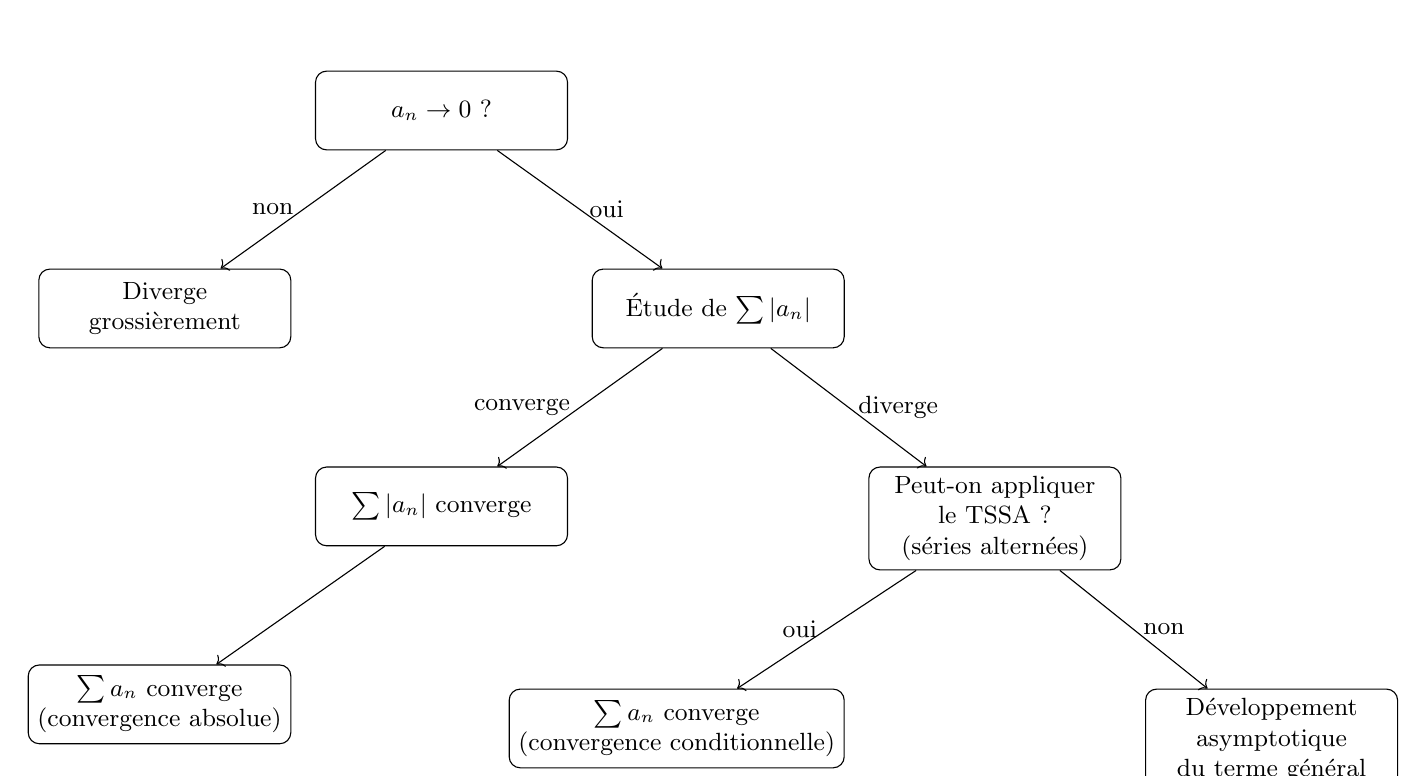
\begin{tikzpicture}[
    scale=0.85, % Réduction légère de l'échelle
    node distance=1.5cm and 0.3cm, % Espacement réduit
    every node/.style={align=center},
    box/.style={draw, rounded corners, minimum width=3.2cm, minimum height=1cm, font=\small} % Bulles un peu plus petites
]

% Structure en arbre vertical
% Niveau 1 : Point de départ
\node[box] (start) {$a_n \to 0$ ?};

% Niveau 2 : Première bifurcation
\node[box, below left=of start] (div) {Diverge\\grossièrement};
\node[box, below right=of start] (absstudy) {Étude de $\sum |a_n|$};

% Niveau 3 : Deuxième bifurcation depuis absstudy
\node[box, below left=of absstudy] (absconv) {$\sum |a_n|$ converge};
\node[box, below right=of absstudy] (applytssa) {Peut-on appliquer\\le TSSA ?\\(séries alternées)};

% Niveau 4 : Conclusions finales
\node[box, below left=of absconv] (seriecv1) {$\sum a_n$ converge\\(convergence absolue)};
\node[box, below left=of applytssa] (seriecv2) {$\sum a_n$ converge\\(convergence conditionnelle)};
\node[box, below right=of applytssa] (devtg) {Développement\\asymptotique\\du terme général};

% Flèches de l'arbre
\draw[->] (start) -- node[left, font=\small]{non} (div);
\draw[->] (start) -- node[right, font=\small]{oui} (absstudy);

\draw[->] (absstudy) -- node[left, font=\small]{converge} (absconv);
\draw[->] (absstudy) -- node[right, font=\small]{diverge} (applytssa);

\draw[->] (absconv) -- (seriecv1);
\draw[->] (applytssa) -- node[left, font=\small]{oui} (seriecv2);
\draw[->] (applytssa) -- node[right, font=\small]{non} (devtg);

\end{tikzpicture}
\end{center}

\vspace{1em}

\noindent
\textbf{Rappels de comparaison asymptotique :}

\begin{itemize}
  \item Si $a_n = b_n + O(w_n)$ où $\sum |w_n|$ converge, 
  alors $\displaystyle \sum_{n\geqslant0} a_n$ et $\displaystyle \sum_{n\geqslant0} b_n$ sont de même nature.

  \item Si $a_n = b_n + c_n + o(c_n)$ où $\sum b_n$ converge et $c_n > 0$, 
  alors $\displaystyle \sum_{n\geqslant0} a_n$ et $\displaystyle \sum_{n\geqslant0} c_n$ sont de même nature.
\end{itemize}

\begin{exemple}
    Soit $n \geqslant 2$, posons $\displaystyle a_n = \frac{(-1)^n}{n + (-1)^n\sqrt{n}}$.
    Étudions $\sum a_n$.

    $\abs{a_n} \sim \frac 1 n$, terme général d'une série divergente donc pas de convergence absolue. 

    $\displaystyle \frac 1 {n + (-1)^n \sqrt n}$ n'est pas décroissante, on ne peut pas appliquer le TSSA. 

    \begin{align*}
        a_n & = \frac{(-1)^n} n \left[ \frac 1 {1 + \frac{(-1)^n} {\sqrt n}} \right] \\
            & = \frac{(-1)^n} n \left[ 1 - \frac{(-1)^n}{\sqrt n} + o\left( \frac 1 {\sqrt n} \right) \right] \\
            & = \underbrace{\frac{(-1)^n} n}_{\text{TGSCV par TSSA}} - \underbrace{\frac 1 {n^{3/2}} + o\left( \frac 1 {n^{3/2}} \right)}_{TGSCV}
    \end{align*}
    
    Donc $\sum a_n$ converge.
\end{exemple}

\begin{exemple}
    Soit $u_n = \sin(n! \pi e)$ et $v_n = \sin(2 n! \pi e)$, $\displaystyle e = \sum_{k = 0 }^{ + \infty } \frac{1}{k!}$

    Donc :
    \begin{align*}
        n! e & = \sum_{k = 0 }^{+ \infty } \frac{n!}{k!} \\
             & = \underbrace{\sum_{k = 0}^{n - 2} \frac{n!}{k!}}_{\substack{P_n \text{ somme} \\ \text{d'entiers pairs}}} + n + 1 + \frac{1}{n + 1} + \frac{1}{(n + 1)(n + 2)} + \frac 1 {(n + 1)(n + 2)(n + 3)} + \sum_{k = n + 4 }^{+ \infty } \frac{n! }{k!} \\
    \end{align*}

    $\displaystyle \forall k \geqslant n + 4$, $\displaystyle \frac{n!}{k!} = \frac{1}{(n + 1)(n + 2) \cdots (k)} \leqslant \frac{1}{(n + 1)(n + 2)\ldots(k - 1)k}$

    \begin{align*}
        \sum_{k = n + 4 }^{+ \infty } \frac{n! }{k!} & \leqslant \sum_{k = n + 4 }^{+\infty}\frac 1 {(n + 1)(n + 2) (k-1)k} \\
                                                     & \leqslant \frac 1 {(n + 1)(n + 2)} \underbrace{\sum_{k = 2}^{+\infty} \frac 1 {(k - 1)k}}_C \\
    \end{align*}

    Donc $n ! e = q_n + \frac 1 {n + 1} + O\left(\frac 1 {n^2}\right)$, $q_n = P_n + n + 1$. Donc :

    \begin{align*}
        \sin(2 \pi n! e) & = \sin \left( 2 \pi \left( q_n + \frac 1 {n + 1} + O\left( \frac 1 {n^2} \right) \right) \right) \\
                         & = \sin \left( 2 \pi \left( \frac 1 {n + 1} + O\left( \frac 1 {n^2} \right) \right) \right) \\
                         & = \frac {2 \pi}{n + 1} + O\left( \frac 1 {n^2} \right) \\
    \end{align*}

    Donc $\sum v_n$ diverge.
    
    \begin{align*}
        \sin(n! \pi e) & = \sin \left( \pi \left( q_n + \frac 1 {n + 1} + O\left( \frac 1 {n^2} \right) \right) \right) \\
                       & = \sin \left( \pi \left( \frac 1 {n + 1} + O\left( \frac 1 {n^2} \right) \right) \right) \\
                       & = (-1)^{q_n} \left( \frac{\pi}{n + 1} + O\left( \frac 1 {n^2} \right) \right) \\
    \end{align*}

    Or, $q_n$ est de parité alternante donc par le TSSA, $\sum u_n$ converge.
\end{exemple}

\subsection{Sommation des relations de comparaison pour les séries divergentes}

Soient $\sum u_n$ et $\sum v_n$ deux séries réelles telles que $(v_n)$ est de signe constant à partir 
d'un certain rang. 

\marginenote{Un peu d'histoire \!}{Les notations $o$ et $O$ viennent du mathématicien allemand Landau.}

\begin{proposition}{Sommation des relations de comparaison}{}
    Si $\sum v_n$ diverge ($v_n$ de signe constant à partir d'un certain rang) et si $u_n = O(v_n)$ (resp $u_n = o(v_n)$, resp $u_n \sim v_n$),
    alors :
    
    \[\sum_{k = 1 }^{n }u_k = O\left( \sum_{k = 1}^{n} v_k \right)\]
    (resp $o$, resp $\sim$).
\end{proposition}

\begin{proof} $v_n > 0$ à partir d'un certain rang.
    
    \uline{Cas du O :}

    \svspace On suppose que $\exists M \in \R$, $\forall n \geqslant n_0, \, \abs{u_n} \leqslant M v_n$.
    Alors :
    \begin{align*}
        \abs{\sum_{k = 0 }^{n } u_k} & \leqslant \sum_{k=0 }^{n } \abs{u_k} \\
                                    & \leqslant \sum_{k = 0}^{n_0 - 1} \abs{u_k} + \sum_{k = n_0}^{n } M v_k \\
                                    & \leqslant \sum_{k = 0}^{n_0 - 1} \abs{u_k - M v_k} + M \sum_{k = 0}^{n } v_k \\
    \end{align*} 

    Or $\sum v_n$ diverge et $v_n > 0$ à partir d'un certain rang donc $\sum_{k = 0}^{n } v_k \to + \infty$.

    \svspace Donc $\displaystyle \frac{\sum_{k = 0 }^{n_0 - 1} (\abs{u_k} - M v_k)}{\sum_{k = 0}^n v_k} \to 0 \leqslant 1$ pour $n > n_1$.

    \svspace Donc pour $\displaystyle n \leqslant \max(n_0, n_1)$, $\displaystyle \abs{\sum_{k = 0 }^{n } u_k} \leqslant \left( 1 + M \right) \sum_{k = 0}^{n } v_k$.

    Donc $\displaystyle \sum_{k = 0}^{n } u_k = O\left( \sum_{k = 0}^{n } v_k \right)$. \\

    \uline{Cas de $o$ :}

    \svspace On suppose que $\forall \varepsilon > 0, \exists n_0 \in \N, \, \forall n \geqslant n_0, \, \abs{u_n} \leqslant \varepsilon v_n$.
    Soit $\varepsilon > 0$. 

    Par le même calcul, $\exists n_0 \in \N, \, \exists n_1 \in \N$ tel que 

    \[\abs{\sum_{k = 0 }^{n } u_k} \leqslant \sum_{k = 0}^{n_0 - 1} (\abs{u_k} - \varepsilon v_k) + \varepsilon \sum_{k = 0}^{n } v_k\]

    et $\displaystyle \frac{\sum_{k = 0 }^{n_0 - 1} (\abs{u_k} - \varepsilon v_k)}{\sum_{k = 0}^{n } v_k} \leqslant \varepsilon$ 

    \svspace Donc pour $n \geqslant \max(n_0, n_1)$, $\displaystyle \abs{\sum_{k = 0 }^{n } u_k} \leqslant 2 \varepsilon \sum_{k = 0}^{n } v_k$.

    Donc $\displaystyle \sum_{k = 0}^{n } u_k = o\left( \sum_{k = 0}^{n } v_k \right)$. \\

    \uline{Cas de $\sim$ :}

    \svspace Supposons que $u_n \sim v_n$.

    Alors $\displaystyle u_n - v_n = o(v_n)$, donc $\displaystyle \sum_{k = 0}^{n } (u_k - v_k) = o\left( \sum_{k = 0}^{n } v_k \right)$.

    Donc $\displaystyle \sum_{k = 0}^{n } u_k = \sum_{k = 0}^{n } v_k + o\left( \sum_{k = 0}^{n } v_k \right) \sim \sum_{k = 0}^{n } v_k$.
\end{proof} 

\begin{proposition}{de Cesàro}{}
    Soit $(a_n)$ telle que $a_n \to \ell \in \overline \R$. Alors :
    \[\frac 1 n \sum_{k = 1}^{n } a_k \to \ell\]
\end{proposition}

\idee{Sommation des relations de comparaison.}

\begin{proof}
    \uline{Si $\ell \in \R^*$}, posons $v_n = \ell$, alors $\sum v_n$ diverge et $(v_n)$ est de signe constant.

    Or $\displaystyle a_n \sim v_n$ donc $\displaystyle \sum_{k = 1}^{n } a_k \sim \sum_{k = 1}^{n } v_k = n \ell$ (sommation des relations de comparaison). 

    Donc $\displaystyle \frac 1 n \sum_{k = 1}^{n } a_k \longrightarrow \ell$.

    \uline{Si $\ell = 0$}, alors $a_n = o(1)$, posons $v_n = 1$.
    De même, $\displaystyle \sum_{k = 1}^{n } a_k = o(n)$ donc $\displaystyle \frac 1 n \sum_{k = 1}^{n } a_k \longrightarrow 0$. \\

    \uline{Si $\ell = + \infty$ :} 

    \svspace Alors $a_n > 0 $ à partir d'un certain rang, et donc $1 = o(a_n)$.

    De même, $\displaystyle n = \sum_{k = 1}^{n } 1 = o\left( \sum_{k = 1}^{n } a_k \right)$ 

    Donc $\displaystyle 1 = o\left( \frac 1 n \sum_{k = 1}^{n } a_k \right)$ donc $\displaystyle \frac 1 n \sum_{k = 1}^{n } a_k \longrightarrow + \infty$.
\end{proof}

\begin{exemple}
    Pour obtenir un équivalent d'une somme partielle de série à termes positifs, 
    on peut espérer le trouver en utilisant la comparaison série intégrale.

    $\alpha > 0$, $\displaystyle S_n = \sum_{k = 0 }^{n } k^\alpha$. 

    Pour $\alpha = 1$, $\displaystyle S_n = \sum_{k = 0 }^{n } k = \frac{n(n + 1)}{2} \sim \frac{n^2}{2}$.

    Pour $\alpha = 2$, $\displaystyle S_n = \sum_{k = 0 }^{n } k^2 = \frac{n(n + 1)(2n + 1)}{6} \sim \frac{n^3}{3}$.

    Pour $\alpha = 3$, $\displaystyle S_n = \sum_{k = 0 }^{n } k^3 = \left( \frac{n(n + 1)}{2} \right)^2 \sim \frac{n^4}{4}$.

    Montrons qu'en général, $\displaystyle S_n \sim \frac{n^{\alpha + 1}}{\alpha + 1}$.

    Soit $k \geqslant 0$, $t \in [k, k + 1], \, k^\alpha \leqslant t^\alpha \leqslant (k + 1)^\alpha$.

    En intégrant sur $[k, k + 1]$, on trouve : $\ds k^\alpha \leqslant \int_{k}^{k + 1} t^\alpha \dt \leqslant (k + 1)^\alpha$

    Divisons par $k^\alpha$ : 
    \[1 \leqslant \frac 1 {k^\alpha} \int_{k}^{k + 1} t^\alpha \dt \leqslant \left( \frac{k+1} k \right)^\alpha \longrightarrow 1\]

    Donc $\ds k^\alpha \sim \int_{k }^{k + 1} t^\alpha \dt$, or $\ds \sum_{k \geqslant 0 } k^\alpha$ série à termes positifs divergente. 

    Donc par sommation des relation de comparaison, 
    \[S_n \sim \sum_{k = 0}^{n } \int_{k}^{k + 1} t^\alpha \dt \sim \frac{n^{\alpha + 1}}{\alpha + 1}\]
\end{exemple}

\begin{remarque}
Pour généraliser cette idée il faut $f\in  \mathscr C^{pm}(\R^+, \R^+)$ monotone telle que $f(k+1) \sim f(k)$, on
montrerait de la même manière, dans le cas où $\ds\int_0^n f(t) \dt$ diverge, que $\ds \sum_{k=1}^n f(k) \sim \int_0^n f(t) \dt$.
\end{remarque}

\subsection{Sommation des relations de comparaison pour des séries convergentes}

\begin{theoreme}{Sommation des relations de comparaison}{}\\
    Soient $\sum u_n$ et $\sum v_n$ deux séries numériques telles que 
    $(v_n)$ est de signe constant à partir d'un certain rang et $\sum v_n$ converge.
    Supposons que $u_n = O(v_n)$ (resp $u_n = o(v_n)$, resp $u_n \sim v_n$).

    \svspace Alors $\sum u_n$ converge et on peut donc définir les restes des deux séries, et 
    $\displaystyle R_n(u) = O(R_n(v))$ (resp $o$, resp $\sim$).
\end{theoreme}

\begin{proof}
    La convergence de $\sum u_n$ est immédiate par comparaison. 

    \uline{Si $u_n =  O(v_n)$}, alors $\exists M > 0, \exists n_0 \in \N, \, \forall k \geqslant n_0, \, \abs{u_k} \leqslant M \abs{v_k}$.

    Donc $\displaystyle \forall n \geqslant n_0, \, \forall N > n, \, \abs{\sum_{k = n + 1 }^{N } u_k} \leqslant \sum_{k = n + 1 }^{N } \abs{u_k} \leqslant M \sum_{k = n + 1}^{N } \abs{v_k}$.

    Par passage à la limite, $\abs{R_n(u)} \leqslant M \abs{R_n(v)}$ car $v_k$ de signe constant. 
    Donc $R_n(u) = O(R_n(v))$. \\

    \uline{Si $u_n = o(v_n)$,} 
    on fait le même raisonnement avec $\forall \varepsilon$ à la place de $\exists M$. \\

    \uline{Si $u_n \sim v_n$}, alors $u_n - v_n = o(v_n)$. 

    Donc $R_n(u - v) = o(R_n(v))$ donc $R_n(u) = R_n(v) + o(R_n(v)) \sim R_n(v)$.
\end{proof}

\begin{exemple}
    Cherchons l'équivalent du reste d'une série de Riemann convergente. 

    Soit $\alpha > 1$, $\displaystyle \sum_{k = n + 1}^{+ \infty } \frac 1 {k^\alpha}$.

    Posons $\displaystyle v_k = \int_k^{k + 1} \frac 1 {t^\alpha} \text d t$. 

    $\displaystyle \forall t \in [k, k + 1], \, \frac 1 {(k + 1)^\alpha} \leqslant \frac 1 {t^\alpha} \leqslant \frac 1 {k^\alpha}$

    Donc $\displaystyle \left( \frac k {k +  1} \right)^\alpha \leqslant \frac {v_k}{u_k} \leqslant 1$.

    Donc $v_k \sim u_k$.
    Donc $R_n(u) \sim R_n(v)$, or :
    \begin{align*}
        \sum_{k = n + 1 }^{N } v_k & = \sum_{k = n + 1}^{N } \int_k^{k + 1} \frac 1 {t^\alpha} \text d t \\
                                   & = \int_{n + 1}^{N + 1} \frac 1 {t^\alpha} \text d t \\
                                   & = \left[ \frac{t^{1 - \alpha}}{1 - \alpha} \right]_{n + 1}^{N + 1} \\
                                   & = \frac 1 {\alpha - 1} \left( \frac 1 {(n + 1)^{\alpha - 1}} - \frac 1 {N + 1}^{\alpha - 1} \right) \\
                                   & \sim \frac 1 {\alpha - 1} \frac 1 {(n + 1)^{\alpha - 1}} 
    \end{align*}

    Donc $\displaystyle \sum_{k = n + 1}^{+ \infty} \frac 1 {k^\alpha} \sim \frac 1 {\alpha - 1} \frac 1 {(n + 1)^{\alpha - 1}}$. \\
\end{exemple}     

\begin{exemple}
    Trouvons maintenant l'équivalent de $\displaystyle \sum_{k = n + 1}^{+ \infty } \frac 1 {k^2} = R_n$.
    On a $\displaystyle \frac 1 {k^2} \sim \frac 1 {k(k + 1)}$.

    Or $\displaystyle \sum_{k = n + 1}^{N} \frac 1 {k(k + 1)} = \sum_{k = n + 1}^{N } \left( \frac 1 k - \frac 1 {k + 1} \right) = \frac 1 {n + 1} - \frac 1 {N + 1}$

    Donc $\displaystyle R_n \sim \frac 1 n$.
    Or par sommation des relations de comparaison, 
    
    \[\sum_{k = n + 1}^{+\infty} \frac 1 {k^2} \sim \sum_{k = n + 1}^{+ \infty } \frac 1 {k(k + 1)} \sim \frac 1 {n + 1} \sim \frac 1 n\]
\end{exemple}

\passerenmodeexos
\section{Énoncés des Exercices}
\subsection{Séries numériques}

% --- (Source: EXERCICE 7 analyse) ---
\begin{exercice}[Exercice 7 Analyse]
\begin{enumerate}
    \item Soient $(u_{n})$ et $(v_{n})$ deux suites de nombres réels positifs.
        On suppose que $(v_{n})$ est non nulle à partir d'un certain rang.
        
        Montrer que si $u_n \sim v_n$ alors $\sum u_n$ et $\sum v_n$ sont de même nature.

    \item Étudier la convergence de la série:
        \[\sum_{n\geqslant2}\frac{(i-1)\ln n \sin\left(\frac{1}{n}\right)}{(\sqrt{n+3}-1)}\]
        (où $i$ est le complexe tel que $i^2 = -1$).
\end{enumerate}
\end{exercice}

% --- (Source: EXERCICE 46 analyse) ---
\begin{exercice}[Exercice 46 Analyse]
    On considère la série $\sum_{n\geqslant1}\cos\left(\pi\sqrt{n^{2}+n+1}\right)$.
    \begin{enumerate}
        \item Prouver que, au voisinage de $+\infty$, $\pi\sqrt{n^{2}+n+1}=n\pi+\frac{\pi}{2}+\alpha\frac{\pi}{n}+O\left(\frac{1}{n^{2}}\right)$ 
            où $\alpha$ est un réel que l'on déterminera.
        \item En déduire que $\sum_{n\geqslant1}\cos\left(\pi\sqrt{n^{2}+n+1}\right)$ converge.
        \item La série converge-t-elle absolument ?
    \end{enumerate}
\end{exercice}

% --- (Source: Exercice 1) ---
\begin{exercice}
\begin{enumerate}
    \item Pour $s\in\C$ tel que $\text{Re}(s)>1$, justifier la convergence absolue de la série de Riemann de somme :
        \[\zeta(s)=\sum_{n=1}^{+ \infty}\frac{1}{n^{s}}\]

    \item Pour $s\in\R$ tel que $s>0$, justifier la convergence de la série alternée de Riemann de somme :
        \[A(s)=\sum_{n=1}^{+ \infty}\frac{(-1)^{n}}{n^{s}}\]
    
    \item  Pour $s\in\C$ tel que $\text{Re}(s)>1$, simplifier $A(s)+\zeta(s)$ et en déduire un lien entre $\zeta(s)$ et $A(s)$.
    \item On s'intéresse à la convergence de $A(s)$ pour $s$ complexe tel que $\text{Re}(s)>0$.
        On fixe $s=a+ib$ avec $a>0$ et $b\in\R$ et on pose $u_{n}=\frac{(-1)^{n}}{n^{s}}$. 
        On note $v_{n}=\text{Re}(u_{n})$ et $w_{n}=\text{Im}(u_{n})$.
    \begin{enumerate}
        \item On pose $V_{n}=v_{2n}+v_{2n+1}$. En montrant que $\frac{1}{(2n+1)^{a}}=\frac{1}{(2n)^{a}}+O\left(\frac{1}{n^{1+a}}\right)$, 
            montrer que la série $\sum V_{n}$ est absolument convergente.
        \item En déduire que la série $\sum v_{n}$ converge.
        \item Conclure en raisonnant de même avec $\sum w_{n}$.
    \end{enumerate}
\end{enumerate}
\textit{Note : Il existait une question 5 qui évoquait de prouver l'hypothèse de Riemann, elle n'est pas traitée ici.}
\end{exercice}

% --- (Source: Exercice 2) ---
\begin{exercice}
\begin{enumerate}
    \item
    \begin{enumerate}
        \item Calculer pour $x\in[0,1]$, $\displaystyle\sum_{k=0}^{N}\left(-x^{2}\right)^{k}$.
        \item Intégrer cette égalité sur $[0, 1]$.
        \item En déduire que $\displaystyle\sum_{n=0}^{+\infty}\frac{(-1)^{n}}{2n+1}=\frac{\pi}{4}$.

    \end{enumerate}
    
    \item On définit pour tout $n$, $\displaystyle I_{n}=\int_{0}^{\pi/2}x^{2}\frac{\sin(2nx)}{\sin x} \dx$.
    \begin{enumerate}
        \item Montrer que $\displaystyle I_{n+1}-I_{n}=\int_{0}^{\pi/2}2x^{2}\cos((2n+1)x) \dx$ 
        et en déduire que $I_{n+1}-I_{n}=\frac{(-1)^{n}\pi^{2}}{2(2n+1)}-\frac{4(-1)^{n}}{(2n+1)^{3}}$.
        \item On pose pour $x>0$, $f(x)=\frac{x^{2}}{\sin x}$. Montrer que $f$ se prolonge en 0 en une fonction de classe $\mathscr C^{1}$.
        \item Utiliser une intégration par parties pour montrer que $\displaystyle|I_{n}|\leqslant\frac{|f(\pi/2)|+\int_{0}^{\pi/2}|f^{\prime}(x)| \dx}{2n}$.
        \item En déduire que $\displaystyle\sum_{n=0}^{+\infty}\frac{(-1)^{n}}{(2n+1)^{3}}=\frac{\pi^{3}}{32}$. % Note: PDF says pi^3/32
    \end{enumerate}
\end{enumerate}
\end{exercice}

% --- (Source: Exercice 3) ---
\begin{exercice}
    On pose pour $\theta\in]0,\pi[$, $u_{n}=\frac{\cos n\theta}{n}$.
    \begin{enumerate}
        \item On pose $\displaystyle C_{n}=\sum_{k=0}^{n}\cos(k\theta)$. Montrer que cette suite est bornée.
        \item En remarquant que pour tout $n\geqslant1$, $\cos n\theta=C_{n}-C_{n-1}$ et en considérant sa somme partielle, 
            montrer que la série $\sum u_{n}$ converge.
        \item Montrer que $|\cos(n\theta)|\geqslant \cos^{2}(n\theta)$ et en déduire que la série $\sum u_{n}$ ne converge pas absolument.
    \end{enumerate}
\end{exercice}

% --- (Source: Exercice 4) ---
\begin{exercice}
    Préciser la nature des séries suivantes:
    \[\sum\frac{(-1)^{n}}{3n-1}, \quad \sum\frac{(-1)^{n}}{n^{\alpha}-(-1)^{n}n^{\beta}} \ (\alpha\ne\beta), \quad \sum \ln\left(1+(-1)^{n}\frac{\ln n}{n^{\alpha}}\right) \ (\alpha>0)\]
\end{exercice}

% --- (Source: Exercice 5 - Stirling) ---
\begin{exercice}
    Montrer que pour tout naturel $n$, $n!e=p_{n}+\frac{1}{n+1}+O\left(\frac{1}{n^{2}}\right)$ 
    où $p_{n}$ est un entier dont on précisera la parité en fonction de $n$.
    En déduire la nature des séries $\sum \sin(n!2\pi e)$ et $\sum \sin(n!\pi e)$.
\end{exercice}

% --- (Source: Exercice 6 - Cesaro) ---
\begin{exercice}
Soit $(\sum u_{n})$ une série numérique convergente. On pose $\displaystyle S_{n}=\sum_{k=0}^{n}u_{k}$.
\begin{enumerate}
    \item Exprimer $\displaystyle\sum_{k=1}^{n}ku_{k}$ à l'aide de $\displaystyle\sum_{k=1}^{n}S_{k}$ (utiliser $u_n = S_n - S_{n-1}$).
    \item En déduire que $\displaystyle\lim_{n\rightarrow+\infty}\frac{1}{n}\sum_{k=1}^{n}ku_{k}=0$.
    \item On pose $\displaystyle v_{n}=\frac{1}{n(n+1)}\sum_{k=1}^{n}ku_{k}$.
        Exprimer $\displaystyle\sum_{k=1}^{n}v_{k}$ à l'aide de $S_{n}$.
        En déduire que la série $(\sum v_{n})$ converge et a même somme que $(\sum u_{n})$.
\end{enumerate}
\end{exercice}

\begin{exercice}
Montrer l'existence et calculer : \[\sum_{n=0}^{+\infty} \frac{1}{(3n)!}\]
\end{exercice}
    
\subsection{Séries dans un espace vectoriel normé de dimension finie}

% --- (Source: EXERCICE 40 analyse) ---
\begin{exercice}[Exercice 40 Analyse]
    Soit $\mathcal{A}$ une algèbre de dimension finie admettant $e$ pour élément unité et munie d'une norme telle que $\|uv\| \leqslant \|u\|\|v\|$.
    \begin{enumerate}
        \item Soit $u \in \mathcal{A}$ tel que $\|u\| < 1$.
        \begin{enumerate}
            \item Démontrer que la série $\sum_{n\geqslant1} u^{n}$ est convergente.
            \item Démontrer que $(e-u)$ est inversible et que $\displaystyle (e-u)^{-1}=\sum_{n=0}^{+\infty}u^{n}$.
        \end{enumerate}
        \item Démontrer que, pour tout $u \in \mathcal{A}$, la série $\sum\frac{u^{n}}{n!}$ converge.
    \end{enumerate}
\end{exercice}

% --- (Source: EXERCICE 61 algèbre) ---
\begin{exercice}[Exercice 61 Algèbre]
    On note $\mathcal{M}_{n}(\C)$ l'espace des matrices carrées d'ordre $n$. Pour $A=(a_{i,j})$, on pose $\|A\| = \max_{i,j \in \ninter 1 n} |a_{i,j}|$.
    \begin{enumerate}
        \item Prouver que $\|\cdot\|$ est une norme.
        \item Démontrer que $\|AB\| \leqslant n\|A\|\|B\|$ et $\forall p \in \N^* \|A^p\| \leqslant n^{p-1}\|A\|^p$.
        \item Démontrer que la série $\sum\frac{A^{p}}{p!}$ est absolument convergente. Est-elle convergente ?
    \end{enumerate}
\end{exercice}

% --- (Source: Exercice 7) ---
\begin{exercice}
    Calculer les exponentielles des matrices suivantes:
    \[\begin{pmatrix} 0 & a \\ -a & 0 \end{pmatrix}, \quad \begin{pmatrix} 1 & 1 \\ 0 & 1 \end{pmatrix}\]

\end{exercice}

% --- (Source: Exercice 8) ---
\begin{exercice}
    On pose $A=\begin{pmatrix}3&6\\ 4&1\end{pmatrix}$.
    \begin{enumerate}
        \item Déterminer deux suites $(a_{n})$ et $(b_{n})$ telles que $A^{n}=a_{n}(A-7I_{2})+b_{n}(A+3I_{2})$.
        \item En déduire $\exp(A)$.
    \end{enumerate}
\end{exercice}

% --- (Source: Exercice 9) ---
\begin{exercice}
    Montrer que pour une matrice $A\in \mathcal{M}_{p}(\K)$ de norme suffisamment petite la série $\sum_{n\geqslant0}A^{n}$ est absolument convergente. 
    Montrer que sa somme est l'inverse de $I_{p}-A$.
\end{exercice}

% --- (Source: Exercice 10) ---
\begin{exercice}
    On munit $\mathcal{M}_{p}(\C)$ d'une norme d'algèbre.
    \begin{enumerate}
        \item Pour tout naturel $n$ et tout $k\in\{0,\dots,n\}$ on pose $a_{n,k}=\frac{1}{k!}-\frac{n!}{k!(n-k)!n^{k}}$. 
            Montrer que $a_{n,k}\geqslant0$.
        \item On pose $M_{n}=(I_{p}+\frac{1}{n}A)^{n}$.
        \begin{enumerate}
            \item Montrer que $\displaystyle M_{n}-\sum_{k=0}^{n}\frac{A^k}{k!}$ tend vers 0.
            \item En déduire que la suite $(M_{n})$ converge vers $\exp(A)$.
        \end{enumerate}
    \end{enumerate}
\end{exercice}

\subsection{Séries à termes positifs}

% --- (Source: EXERCICE 5 analyse) ---
\begin{exercice}[Exercice 5 Analyse]
\begin{enumerate}
    \item On considère la série de terme général $u_{n}=\frac{1}{n(\ln n)^{\alpha}}$ ($n\geqslant2, \alpha\in\R$).
    \begin{itemize}
        \item Cas $\alpha\leqslant0$ : En utilisant une minoration simple, démontrer que la série diverge.
        \item Cas $\alpha>0$ : Étudier la nature de la série (comparaison série-intégrale avec $f(x)=\frac{1}{x(\ln x)^{\alpha}}$).
    \end{itemize}
    \item Déterminer la nature de la série $\sum_{n\geqslant3}\frac{\left(e-\left(1+\frac{1}{n}\right)^{n}\right)e^{\frac{1}{n}}}{(\ln(n^{2}+n))^{2}}$.
\end{enumerate}
\end{exercice}

% --- (Source: Exercice 11) ---
\begin{exercice}
    Établir la convergence et calculer la somme de la série télescopique : $\sum_{n\geqslant2}\ln\left(1-\frac{1}{n^{2}}\right)$.
\end{exercice}

% --- (Source: Exercice 12) ---
\begin{exercice}
\begin{enumerate}
    \item Comparer pour $a, b \in \R^{+}$, $\arctan(a) - \arctan(b)$ avec $\arctan \frac{a-b}{1+ab}$.
    \item En déduire la convergence et la somme de $\sum_{n\geqslant1}\arctan\left(\frac{1}{n^{2}+n+1}\right)$.
    \item On définit la suite de Fibonacci $(F_{n})$ par $F_{0}=0, F_{1}=1, F_{n+2}=F_{n}+F_{n+1}$.
    \begin{enumerate}
        \item Montrer la convergence de $\sum_{k\geqslant1}\arctan\left(\frac{1}{F_{2k+1}}\right)$.
        \item Montrer que pour tout $n$, $\displaystyle\frac{\pi}{4}=\sum_{k=1}^{n}\arctan\left(\frac{1}{F_{2k+1}}\right)+\arctan\left(\frac{1}{F_{2n+2}}\right)$.
        \item En déduire que $\displaystyle\sum_{k=1}^{+\infty}\arctan\left(\frac{1}{F_{2k+1}}\right) = \frac{\pi}{4}$.
    \end{enumerate}
\end{enumerate}
\end{exercice}

% --- (Source: Exercice 13) ---
\begin{exercice}
    Soient $a, b, c, d > 0$ et $u_{n}$ telle que $\frac{u_{n+1}}{u_{n}}=\frac{(n+a)(n+b)}{(n+c)(n+d)}$.
    \begin{enumerate}
        \item Pour $\alpha>0$, on pose $v_{n}=\ln(n^{\alpha}u_{n})$. Écrire un développement asymptotique de $v_{n+1}-v_{n}$. 
            À quelle condition la série télescopique converge-t-elle ?
        \item En déduire un équivalent de $u_{n}$.
    \end{enumerate}
\end{exercice}

% --- (Source: Exercice 14) ---
\begin{exercice}
    Si $\sum u_{n}$ converge (à termes positifs), établir la convergence des séries
    \[\sum u_{n}^{2},~ \sum\frac{u_{n}}{1+u_{n}^{2}}, ~\sum\frac{\sqrt{u_{n}}}{n^{\alpha}} ~\text{avec}~ \alpha>\frac{1}{2}\]
\end{exercice}

% --- (Source: analyse) ---
\begin{exercice}
    Soit $(u_{n})$ à termes strictement positifs.
    \begin{enumerate}
        \item Démontrer que si $\lim \frac{u_{n+1}}{u_{n}}=l < 1$, alors $\sum u_{n}$ converge
        \item Quelle est la nature de $\sum_{n\geqslant1}\frac{n!}{n^{n}}$ ?
    \end{enumerate}
\end{exercice}

% --- (Source: Exercice 15 - Raabe Duhamel) ---
\begin{exercice}[Règle de Raabe Duhamel]
\begin{enumerate}
    \item Montrer que si $\sum u_{n}$ et $\sum v_{n}$ sont deux séries à termes positifs 
        telles que pour $n$ assez grand $\frac{u_{n+1}}{u_{n}}\leqslant\frac{v_{n+1}}{v_{n}}$, 
        alors la convergence de $\sum v_{n}$ implique celle de $\sum u_{n}$
    \item On suppose $\frac{u_{n+1}}{u_{n}}=1-\frac{\alpha}{n}+o\left(\frac{1}{n}\right)$. 
        Montrer que $\sum u_{n}$ converge pour $\alpha>1$ et diverge pour $\alpha<1$ (comparer avec $v_n = \frac{1}{n^\beta}$).
\end{enumerate}
\end{exercice}

% --- (Source: Exercice 16) ---
\begin{exercice}
    Trouver la nature des séries :
    \[\sum \frac{1}{\ln(n)^{\ln n}}, \quad \sum \frac {n^n} {2^{n^2}}, \quad \sum \frac{n!^2}{(2n)!}, \quad \sum \left(\sin\frac{1}{n}\right) n^\alpha, \alpha \in \R\]
\end{exercice}

% --- (Source: Exercice 17) ---
\begin{exercice}
    Soit $\sum u_{n}$ une série à termes positifs, $u_0 > 0$. On pose $\displaystyle S_{n}=\sum_{k=0}^{n}u_{k}$.
    \begin{enumerate}
        \item Supposons $\sum u_{n}$ converge. Montrer que $\sum\frac{u_{n}}{S_{n}}$ converge
        \item Supposons $\sum\frac{u_{n}}{S_{n}}$ converge. 
            Trouver la nature de $\sum \ln\left(\frac{S_{n-1}}{S_{n}}\right)$. 
            En déduire que $\sum u_{n}$ converge
        \item Montrer que si $\sum a_{n}$ diverge (termes positifs), 
            il existe $\sum b_{n}$ divergente (à termes positifs) telle que $b_{n}=o(a_{n})$.
    \end{enumerate}
\end{exercice}

% --- (Source: Exercice 18) ---
\begin{exercice}
    Soit $\alpha>1$ et $\displaystyle R_{n}=\sum_{k=n+1}^{+\infty}\frac{1}{k^{\alpha}}$.
    \begin{enumerate}
        \item Déterminer un équivalent de $R_{n}$
        \item Condition nécessaire sur $\alpha$ de convergence de $\sum R_{n}$.
        \item Valeur de la somme dans ce cas ?
    \end{enumerate}
\end{exercice}

\newpage
\section{Corrections}

% --- Correction Exercice 2 (du fichier source, Exercice 46 ici) ---
\begin{correction}{2}
\begin{enumerate}
    \item On fait le calcul :
    \begin{align*}
        \pi\sqrt{n^2+n+1} &= \pi n \left(1 + \frac{1}{n} + \frac{1}{n^2}\right)^{1/2} \\
        &= \pi n \left(1 + \frac{1}{2n} + \frac{3}{8n^2} + O\left(\frac{1}{n^3}\right)\right) \\
        &= \pi n + \frac{\pi}{2} + \frac{3\pi}{8n} + O\left(\frac{1}{n^2}\right).
    \end{align*}
    
    \item $\cos(\pi\sqrt{\dots}) = \cos(n\pi + \pi/2 + \varepsilon_n) = (-1)^n \cos(\pi/2 + \varepsilon_n) = (-1)^{n+1} \sin(\varepsilon_n)$.
    Et $\sin(\varepsilon_n) \sim \frac{3\pi}{8n}$.

    C'est une série alternée $\sum (-1)^{n+1} \frac{K}{n}$. Elle converge (TSSA).
    Absolue convergence ? Non, car en $1/n$.
\end{enumerate}
\end{correction}

% --- Correction Exercice 3 ---
\begin{correction}{3}
\begin{enumerate}
    \item
        Soit $s=a+ib$ avec $a>1$.
        $|\frac{1}{n^s}| = \frac{1}{|n^a e^{ib\ln n}|} = \frac{1}{n^a}$.
        C'est une série de Riemann avec $a>1$, donc convergente. Absolue convergence vérifiée.

    \item 
        Pour $s>0$ réel, la suite $\frac{1}{n^s}$ tend vers 0 en décroissant.
        D'après le Théorème Spécial des Séries Alternées (TSSA), $\sum \frac{(-1)^n}{n^s}$ converge.

    \item 
        $A(s)+\zeta(s) = \sum_{n=1}^{+ \infty} \frac{(-1)^n+1}{n^s}$.
        Si $n$ est impair, $(-1)^n+1=0$. Si $n=2p$ est pair, $(-1)^n+1=2$.
        $$ A(s)+\zeta(s) = \sum_{p=1}^{+ \infty} \frac{2}{(2p)^s} = \frac{2}{2^s} \sum_{p=1}^{+ \infty} \frac{1}{p^s} = 2^{1-s} \zeta(s) $$
        D'où $A(s) = (2^{1-s}-1)\zeta(s)$.

    \item
    \begin{enumerate}
        \item $s=a+ib$ avec $a>0$.
        
            $u_n = \frac{(-1)^n}{n^s} = \frac{(-1)^n}{n^a} \cos(b\ln n) - i \frac{(-1)^n}{n^a} \sin(b\ln n)$.

            Soit $v_n = \text{Re}(u_n)$.
            $V_n = v_{2n} + v_{2n+1} = \frac{1}{(2n)^a}\cos(b\ln(2n)) - \frac{1}{(2n+1)^a}\cos(b\ln(2n+1))$.

            Développement asymptotique :
            $\frac{1}{(2n+1)^a} = \frac{1}{(2n)^a}(1+\frac{1}{2n})^{-a} = \frac{1}{(2n)^a} - \frac{a}{(2n)^{a+1}} + o(\frac{1}{n^{a+1}})$
            
            $\cos(b\ln(2n+1)) = \cos(b\ln(2n) + b\ln(1+\frac{1}{2n})) \approx \cos(b\ln(2n)) - \sin(b\ln(2n))\frac{b}{2n}$.
            
            En combinant, on obtient $V_n = O(\frac{1}{n^{1+a}})$.
            Comme $1+a > 1$, $\sum V_n$ converge absolument.

        \item 
            Puisque $v_n \to 0$, la convergence de $\sum (v_{2n}+v_{2n+1})$ implique celle de $\sum v_n$.

        \item
            Idem pour la partie imaginaire. Donc $A(s)$ converge pour $\text{Re}(s)>0$.
    \end{enumerate}
\end{enumerate}
\end{correction}

% --- Correction Exercice 4 ---
\begin{correction}{4}
\begin{enumerate}
    \item
    \begin{enumerate}
        \item $\displaystyle \sum_{k=0}^N (-x^2)^k = \frac{1-(-x^2)^{N+1}}{1-(-x^2)} = \frac{1-(-1)^{N+1}x^{2N+2}}{1+x^2}$.
        \item 
            En intégrant sur $[0,1]$ :
            $\displaystyle \int_0^1 \sum (-x^2)^k \dx = \sum_{k=0}^N (-1)^k \int_0^1 x^{2k} \dx = \sum_{k=0}^N \frac{(-1)^k}{2k+1}$.

            D'autre part : $\displaystyle\int_0^1 \frac{\dx}{1+x^2} - \int_0^1 \frac{(-1)^{N+1}x^{2N+2}}{1+x^2} \dx = [\arctan x]_0^1 - R_N = \frac{\pi}{4} - R_N$.

            Majoration du reste : $\displaystyle |R_N| \leqslant \int_0^1 x^{2N+2} \dx = \frac{1}{2N+3} \to 0$.
            Donc $\displaystyle \sum_{n=0}^{+\infty} \frac{(-1)^n}{2n+1} = \frac{\pi}{4}$.
    \end{enumerate}
    
    \item
    \begin{enumerate}
        \item 
            $\displaystyle I_{n+1}-I_n = \int_0^{\pi/2} \frac{x^2}{\sin x} (\sin((2n+2)x) - \sin(2nx)) \dx$.
            
            Utilisation de $\sin p - \sin q = 2 \sin\frac{p-q}{2} \cos\frac{p+q}{2}$.
            On a $\displaystyle I_{n+1}-I_n = \int_0^{\pi/2} 2x^2 \cos((2n+1)x) \dx$.

            Par double IPP ou calcul direct, on obtient le résultat donné.

        \item 
            $f(x) = \frac{x^2}{\sin x} \sim_0 x$. $f(0)=0$. $f$ est continue en 0.
            $f'(x) = \frac{2x\sin x - x^2\cos x}{\sin^2 x}$ et tend vers $1$ en $0$.

            Donc par prolongement $\mathscr C^1$, $f$ est $\mathscr C^1$ sur $[0,1]$.

        \item
            Par IPP sur $I_n$ (avec $u=f(x)$ et $v'=\sin(2nx)$), on obtient la majoration en $1/n$ (ou $1/2n$).
            $\sum (I_{n+1}-I_n)$ est une série télescopique qui converge vers $-I_0 = 0$ (car $I_n \to 0$ par Riemann-Lebesgue).

            La somme des termes en $1/(2n+1)$ donne $\pi^2/8$ (pré-requis ?). La somme des termes en $1/(2n+1)^3$ s'en déduit.
        
        \item La correction indique que $\sum \frac{(-1)^n}{(2n+1)^3} = \frac{\pi^3}{32}$.
    \end{enumerate}
\end{enumerate}
\end{correction}

% --- Correction Exercice 6 ---
\begin{correction}{6}
\begin{itemize}
    \item $\sum \frac{(-1)^n}{3n-1}$ : Converge par le TSSA ($1/(3n-1) \searrow 0$). Ne converge pas absolument.
    
    \item $\sum \frac{(-1)^n}{n^\alpha - (-1)^n n^\beta}$ avec $\alpha \neq \beta$.
        Supposons $\alpha > \beta$.
        $u_n = \frac{(-1)^n}{n^\alpha(1 - (-1)^n n^{\beta-\alpha})} = \frac{(-1)^n}{n^\alpha} + \frac{1}{n^{2\alpha-\beta}} + o(\dots)$. \\
        Le terme $\frac{(-1)^n}{n^\alpha}$ est le terme général d'une série convergente (TSSA). \\
        Le terme $\frac{1}{n^{2\alpha-\beta}}$ est de signe constant positif. \\
        La série converge ssi $\sum \frac{1}{n^{2\alpha-\beta}}$ converge, soit $2\alpha - \beta > 1$.

        Si $\alpha < \beta$.
        Le terme général est équivalent à $- \frac 1 {n^{\beta}}$ donc la série converge ssi $\beta > 1$ (série de Riemann).
        
    \item $\sum \ln(1 + \frac{(-1)^n (\ln n)}{n^\alpha})$.
        DL : $u_n = \frac{(-1)^n \ln n}{n^\alpha} - \frac{\ln^2 n}{2 n^{2\alpha}} + \dots$ \\
        Le premier terme converge (TSSA). Le second terme est de signe constant. \\
        La série converge ssi $2\alpha > 1$, donc $\alpha > 1/2$.
\end{itemize}
\end{correction}

\begin{correction}{7}
Soit $n \in \N$, on a la décomposition suivante :
    \[n! e = P_n + R_n  \quad \text{où} \quad P_n = \sum_{k=0}^{n} \frac{n!}{k!} \in \N \quad \text{et} \quad R_n = \frac{1}{n+1} + \sum_{k=n+2}^{+\infty} \frac{n!}{k!} = \frac{1}{n+1} + O\left(\frac{1}{n^2}\right) \] 
    
    Et donc: 
    \[ \sin(n! e 2\pi) = \sin(2\pi P_n + 2\pi R_n) \quad \text{et} \quad \sin(n! e \pi) = \sin(\pi P_n + \pi R_n) \]
    
    Puisque $P_n \in \N$, on a :
    \[ \sin(n! e 2\pi) = \sin(2\pi R_n) \quad \text{et} \quad \sin(n! e \pi) = (-1)^{P_n}\sin(\pi R_n) \]
    
    Or :
    \[\sin(2\pi R_n) \sim 2\pi R_n \sim \frac{2\pi}{n+1} \] 
    
    Par comparaison avec la série harmonique, la série de terme général $\sin(n! e 2\pi)$ diverge. \newline
    
    Mais par récurrence sur $n$ on étudie la parité de $P_n$:
    \begin{itemize}
    \item \text{Initialisation :} 
        Pour $n = 0$, $P_0 = \frac{0!}{0!} = 1$ (impair). 
        Pour $n = 1$, $P_1 = \frac{1!}{0!} + \frac{1!}{1!} = 1 + 1 = 2$ (pair).
    
    \item \text{Hérédité :} Soit $n \in \N$. Par hypothèse de récurrence, on sait que : \\
        $n \equiv 0 \ [2] \implies P_n \equiv 1 \ [2]$ \quad et \quad $n \equiv 1 \ [2] \implies P_n \equiv 0 \ [2]$ \quad Et on a \quad $P_{n+1} = (n+1)P_n + 1$ \\

        Donc, pour n pair, $P_{n+1} = \underbrace{ \underbrace{(n+1)}_{\text{impair}} \underbrace{P_n}_{\text{impair}} + 1}_{\text{pair}}$ 
        et pour n impair, $P_{n+1} = \underbrace{ \underbrace{(n+1)}_{\text{pair}} \underbrace{P_n}_{\text{pair}} + 1}_{\text{impair}}$ 
    \end{itemize}
    Ainsi, selon le principe de récurrence, on en déduit que: $\forall n \in \N, (-1)^{P_n} = (-1)^{n+1}$ \\
    
    Et par le critère des séries spéciales alternées, on en déduit que la série de terme général $\sin(n! \pi e)$ est semi-convergente.    
\end{correction}

\begin{correction}{8}
\begin{enumerate}
    \item ...
    \item On applique Cesàro.
\end{enumerate}
\end{correction}

\begin{correction}{9}
    Notons $S$ la série. On a, pour tout $n\in\N$,
    \[
    0\leq \frac{1}{(3n)!}\leq \frac{1}{n!}.
    \]
    Or, la série exponentielle converge, donc $S$ converge.
    
    Mais pour $j=e^{2i\pi/3}$, on a,
    \[
    e+e^j+e^{j^2}
    =\sum_{k=0}^{+\infty}\frac{1+j^k+j^{2k}}{k!}.
    \]
    
    Or, pour tout $k\in\N$,
    \[
    1+j^k+j^{2k}=
    \begin{cases}
        3 & \text{si } 3\mid k,\\
        0 & \text{sinon}.
    \end{cases}
    \]
    Ainsi,
    \[
    e+e^j+e^{j^2}
    =3\sum_{n=0}^{+\infty}\frac{1}{(3n)!}.
    \]
    
    Puisque $ e^j=e^{-\frac12}e^{i\frac{\sqrt{3}}{2}}
    \quad\text{et}\quad
    e^{j^2}=e^{-\frac12}e^{-i\frac{\sqrt{3}}{2}}.
    \quad\text{et par la relation}\quad
    e^{i\theta}+e^{-i\theta} = 2 \cos \theta
    $.
     
    On a :
    \[
    S = \frac{e+e^j+e^{j^2}}{3}
    = \frac13\left(e+\frac{2}{\sqrt{e}}\cos\left(\frac{\sqrt{3}}{2}\right)\right)
    \]
\end{correction}

\begin{correction}{10}
\begin{enumerate}
    \item
    \begin{enumerate}
        \item $\|u\| < 1$. La série $\sum \|u\|^n$ converge (géométrique). \\
            Donc $\sum u^n$ converge absolument (donc converge car l'espace est complet - dimension finie).
        
        \item $(e-u) \sum_{k=0}^n u^k = e - u^{n+1}$.
            Comme $u^n \to 0$, le produit tend vers $e$. \\
            Donc $(e-u)$ est inversible d'inverse la somme de la série.
    \end{enumerate}
\end{enumerate}
\end{correction}

\begin{correction}{11}
\begin{enumerate}
    \item $\|\cdot\|$ est définie positive.
    Soit $A,B \in \mathscr M_n(\C)$.

    Séparation : $\|0\| = 0$. Supposons que $\|A\| = 0$.

    Alors $\forall i,j \in \ninter 1 n,~|a_{i,j}| \leqslant 0$. Donc $A = 0$.
    
    Homogénéité : soit $\lambda \in \C$,
    \[\|\lambda A\| = \max_{i,j \in \ninter 1 n} |\lambda a_{i,j}| = \lambda \max_{i,j \in \ninter 1 n} |a_{i,j}| = \lambda \|A\|\]

    Inégalité triangulaire :
    \[\|A + B\| = \max_{i,j \in \ninter 1 n} |a_{i,j} + b_{i,j}| \leqslant \max_{i,j \in \ninter 1 n} (|a_{i,j}| + |b_{i,j}|) \leqslant \|A\| + \|B\|\]

    \item Soient $A,B \in \mathscr M_n(\C)$,
    \begin{align*}
        \|AB\| &= \max_{i,j \in \ninter 1 n} \left|\sum_{k=1}^n a_{i,k} b_{k,j}\right| \\
               &\leqslant \max_{i,j \in \ninter 1 n} \sum_{k=1}^n |a_{i,k} b_{k,j}| \\
               &\leqslant \max_{i,j \in \ninter 1 n}\left(n \max_{k \in \ninter 1 n} |a_{i,k}| |b_{k,j}|\right) \\
               &\leqslant n \left(\max_{i,k \in \ninter 1 n} |a_{i,k}|\right) \left(\max_{k,j \in \ninter 1 n} |b_{k,j}|\right) \\
               &\leqslant n \|A\| \|B\|
    \end{align*}

    Par réccurrence immédiate en prenant $B = A$, on obtient que $\forall p \in \N^*,~\|A^p\| \leqslant n^{p-1}\|A\|^p$.

    \item Soit $p \in \N^*$,
    $\frac {\|A^p\|} {p!} \leqslant \frac {n^{p-1}\|A\|^p} {p!} = \frac {(n\|A\|)^p} {p!n}$
    par critère de comparaison, le terme général est en $O\left(\frac 1 {n^2}\right)$ donc la série converge absolument.

    Étant en dimension finie, la série est convergente.
\end{enumerate}
\end{correction}

\begin{correction}{12}
\begin{itemize}
    \item $A = \begin{pmatrix} 0 & a \\ -a & 0 \end{pmatrix}$.
        $A^2 = -a^2 I_2$ et $A^3 = -a^3 J$ (avec $J=\begin{pmatrix} 0 & 1 \\ -1 & 0 \end{pmatrix}$).
        En fait $A = a J$. $J^2 = -I_2$.
            
        $\exp(A) = \sum \frac{A^k}{k!} = \sum (-1)^p \frac{a^{2p}}{(2p)!} I_2 + \sum (-1)^p \frac{a^{2p+1}}{(2p+1)!} J$.

        $\exp(A) = (\cos a) I_2 + (\sin a) J = \begin{pmatrix} \cos a & \sin a \\ -\sin a & \cos a \end{pmatrix}$.
    \item $A = \begin{pmatrix} 1 & 1 \\ 0 & 1 \end{pmatrix} = I_2 + N$ avec $N=\begin{pmatrix} 0 & 1 \\ 0 & 0 \end{pmatrix}$.
        $I_2$ et $N$ commutent. 
        
        $\exp(A) = \exp(I_2)\exp(N) = e (I_2+N) = \begin{pmatrix} e & e \\ 0 & e \end{pmatrix}$.
\end{itemize}
\end{correction}

\begin{correction}{13}
\begin{enumerate}
    \item $A = \begin{pmatrix} 3 & 6 \\ 4 & 1 \end{pmatrix}$. Polynôme caractéristique : $X^2 - 4X - 21 = (X-7)(X+3)$.
        Valeurs propres $7$ et $-3$.

        $A^n = \alpha_n A + \beta_n I$. Ou système avec les valeurs propres.
        $7^n = 7a_n + b_n$ (système adapté à la décomposition de l'énoncé).

        On trouve $A^n = \frac{1}{10} [ 7^n (A+3I) - (-3)^n (A-7I)]$.

    \item On a immédiatement $\exp(A) = \frac{e^7}{10}(A+3I) - \frac{e^{-3}}{10}(A-7I)$.
\end{enumerate}
\end{correction}

\begin{correction}{15}
\begin{enumerate}
    \item $a_{n,k} = \frac{1}{k!} \left(1 - \frac{n(n-1)\dots(n-k+1)}{n^k} \right)$.
        Or $\frac{n}{n} \dots \frac{n-k+1}{n} \leqslant 1$. Donc $a_{n,k} \ge 0$.
    
    \item
    \begin{enumerate}   
        \item $\displaystyle M_n = \left(I + \frac A n \right)^n = \sum_{k=0}^n \binom{n}{k} \frac{A^k}{n^k} = \sum_{k=0}^n \frac{1}{k!} \frac{n!}{n^k(n-k)!} A^k$.

            Différence : $\displaystyle D_n = - \sum_{k=0}^n a_{n,k} A^k$
            En norme : $\displaystyle \|D_n\| \leqslant \sum_{k=0}^n a_{n,k} \|A\|^k = \sum_{k=1}^n a_{n,k} ||A||^k$.

            Refaire le calcul avec $||A||$ revient au même donc $\displaystyle||D_n|| \leqslant \left(1 + \frac {||A||} n\right)^n - \sum_{k=0}^n \frac {||A||^k} {k!}$.

            On utilise l'exponentielle réelle : $\left(1+\frac{\|A\|}{n}\right)^n \to e^{\|A\|}$.
            L'autre aussi, donc la différence tend vers 0.

        \item On en déduit directement que $M_n \to \exp(A)$.
    \end{enumerate}
\end{enumerate}
\end{correction}

\begin{correction}{17}

    $|u_n| \sim \frac 1 {n^2}$. Donc la série converge.

    Calculons les sommes partielles :
    $$\sum_{k=2}^n \ln(k^2 - 1) - \ln(k^2) = \sum_{k=3}^{n+1} \ln(k) + \sum_{k=1}^{n-1} \ln(k) - 2 \sum_{k=2}^{n} \ln(k) = \ln(1 + \frac 1 n) - \ln(2)$$
    Donc la somme est $-\ln(2)$.
\end{correction}

\begin{correction}{19}
\begin{enumerate}
    \item   
        $u_n > 0$. $\frac{u_{n+1}}{u_n} = \frac{(n+a)(n+b)}{(n+c)(n+d)} \to 1$. Cas douteux d'Alembert.

        $v_n = \ln(n^\alpha u_n)$.
        $v_{n+1}-v_n = \alpha \ln(1+\frac{1}{n}) + \ln \frac{u_{n+1}}{u_n}$.

        DL de $\frac{u_{n+1}}{u_n} = 1 + \frac{a+b-c-d}{n} + O\left(\frac{1}{n^2}\right)$.
        $v_{n+1}-v_n = \frac{\alpha + a+b-c-d}{n} + O\left(\frac{1}{n^2}\right)$.

        Série télescopique converge ssi le terme en $1/n$ est nul.
        Condition : $\alpha = c+d-a-b$.

    \item Si cette condition est remplie, $v_n \to L$.
        Donc $n^\alpha u_n \to e^L$,
        donc $u_n \sim \frac{K}{n^{c+d-a-b}}$.
\end{enumerate}
\end{correction}

\begin{correction}{22}
\begin{enumerate}
    \item Si $\frac{u_{n+1}}{u_n} \leqslant \frac{v_{n+1}}{v_n}$, alors $\frac{u_{n+1}}{v_{n+1}} \leqslant \frac{u_n}{v_n}$.
        La suite $(u_n/v_n)$ est décroissante, donc bornée.
        
        $u_n = O(v_n)$. Si $\sum v_n$ converge, alors $\sum u_n$ converge.
        
    \item Comparaison avec Riemann $v_n = \frac{1}{n}^\beta$.

        $\frac{v_{n+1}}{v_n} = \left(1+\frac{1}{n}\right)^{-\beta} = 1 - \frac{\beta}{n} + o\left(\frac{1}{n}\right)$.
        Si $\frac{u_{n+1}}{u_n} = 1 - \frac{\alpha}{n} + o(\frac{1}{n})$.
    \begin{itemize}
        \item Si $\alpha > 1$, on peut choisir $\beta$ tel que $1 < \beta < \alpha$.

            Alors pour $n$ grand, $1 - \frac{\alpha}{n} < 1 - \frac{\beta}{n}$, donc $\frac{u_{n+1}}{u_n} < \frac{v_{n+1}}{v_n}$.
            $\sum v_n$ converge (Riemann $\beta>1$), donc $\sum u_n$ converge.

        \item Si $\alpha < 1$, divergence par comparaison avec $\beta \in ]\alpha, 1[$.
    \end{itemize}
\end{enumerate}
\end{correction}

\begin{correction}{23}
\begin{itemize}
    \item $u_n = \frac 1 {n^{\ln(\ln(n))}} \leqslant \frac 1 {n^2}$ pour $n$ assez grand donc elle converge. 
    \item $u_n = \frac{n^n}{e^{n^2}}$. $n^2 u_n \to 0$. Donc elle converge (racine n-ième).
    \item $u_n = \frac{n!^2}{(2n)!}$. Stirling : $\frac{n^{2n} e^{-2n} (2\pi n)}{(2n)^{2n} e^{-2n} \sqrt{4\pi n}} \sim \frac{\sqrt{\pi n}}{4^n}$. D'Alembert. Converge

    \item $u_n = (\sin \frac{1}{n}) n^\alpha \sim n^{\alpha-1}$. Converge ssi $1-\alpha > 1 \iff \alpha < 0$. 
    
        (Attention, énoncé dit $e^{n^\alpha \ln(...)}$, vérifier l'énoncé exact, correction mentionne exponentielle).
        L'énoncé PDF source mentionne $\sum (\sin \frac{1}{n}) n^\alpha$.
        La correction manuscrite traite $u_n = e^{n^\alpha \ln(n \sin(1/n))}$.

        $n \sin(1/n) = 1 - \frac{1}{6n^2}$.
        $\ln(\dots) \sim -\frac{1}{6n^2}$.

        Exposant $\sim - \frac{n^{\alpha-2}}{6}$.
        \begin{itemize}
            \item Si $\alpha < 2$, exposant $\to 0$, $u_n \to 1$. Diverge.
            \item Si $\alpha = 2$, $u_n \to e^{-1/6}$. Diverge.
            \item Si $\alpha > 2$, exposant $\to -\infty$ (très vite ? ou vers 0 par valeurs négatives ?).
        \end{itemize}
        Attention, il y a $n^\alpha$ en facteur devant le log dans l'exposant.

        Si $\alpha > 2$, $n^{\alpha-2} \to +\infty$, terme $\to e^{-\infty} = 0$.
        Règle $n^2 u_n$.
\end{itemize}
\end{correction}

\begin{correction}{24}
\begin{enumerate}
    \item Si $\sum u_n$ converge, $S_n \to S > 0$. Donc $u_n/S_n \sim u_n/S$. Converge.
    \item Si $\sum u_n/S_n$ converge.
        $\ln(\frac{S_n}{S_{n-1}}) = \ln(1 + \frac{u_n}{S_{n-1}}) \approx \frac{u_n}{S_{n-1}} \approx \frac{u_n}{S_n}$.

        La série $\sum \ln(S_n) - \ln(S_{n-1})$ est de même nature que $\sum u_n/S_n$.
        C'est une somme télescopique $\ln S_n$.

        Si elle converge, $\ln S_n$ a une limite, donc $S_n$ a une limite finie. $\sum u_n$ converge.
\end{enumerate}
\end{correction}

\begin{correction}{25}
\begin{enumerate}
    \item 
        $\displaystyle R_n = \sum_{k=n+1}^{+\infty} \frac{1}{k^\alpha}$.
        Comparaison série-intégrale : $\displaystyle R_n \sim \int_n^{+\infty} \frac{\dt}{t^\alpha} = \frac{1}{(\alpha-1)n^{\alpha-1}}$.
        
    \item $\sum R_n$ converge ssi $\sum \frac{1}{n^{\alpha-1}}$ converge
        ssi $\alpha-1 > 1 \iff \alpha > 2$.

    \item Somme : 
        \begin{align*}
            \sum_{n=1}^{+\infty} R_n &= \sum_{n=1}^{+\infty} \sum_{k=n+1}^{+\infty} \frac{1}{k^\alpha} \\
                &= \sum_{k=2}^{+\infty} \frac{1}{k^\alpha} \sum_{n=1}^{k-1} 1 \\
                &= \sum_{k=2}^{+\infty} \frac{k-1}{k^\alpha} \\
                &= \zeta(\alpha-1) - \zeta(\alpha) &&
        \end{align*}
\end{enumerate}
\end{correction}




\pagevide
\chapitreintegral{5}{Familles sommables}
\displaychapitrebanner
\section{Dénombrabilité}
\subsection{Définitions}

\begin{definition}{Dénombrable}{}
    Soit $I$ un ensemble. On dit que $I$ est \emph{dénombrable} 
    s'il existe une bijection entre $\N$ et $I$.
    On dira que $I$ est \emph{équipotent} à $\N$ (LHP).
\end{definition}

\begin{exemple}
    \begin{itemize}
        \item L'ensemble $\N$ est dénombrable (la bijection est l'identité).
        \item L'ensemble $\N^*$ est dénombrable (la bijection est $f : n \mapsto n+1$).
        \item $2 \N$ est dénombrable (la bijection est $f : n \mapsto 2n$).
        \item $\Z$ est dénombrable (la bijection est $f : n \mapsto p \text{ ou } -p-1$ selon la parité de $n$).
    \end{itemize}
\end{exemple}

\begin{definition}{Au plus dénombrable}{}
    Soit $I$ un ensemble. On dit que $I$ est \emph{au plus dénombrable} si $I$ est 
    fini ou dénombrable.
\end{definition}

\subsection{Cas des parties de \texorpdfstring{$\N$}{N}}

\begin{theoreme}{Nature des parties infinies de $\N$}{}
    Toute partie infinie de $\N$ est dénombrable.
\end{theoreme}

\idee{
    On numérote les éléments de $A$ par ordre croissant en construisant une 
    bijection et des récurrences.
}

\begin{proof}
    Soit $A \subset \N$ infinie. 

    Construisons par récurrence $\varphi : \N \to A$ en posant : $\varphi(0) = \min(A)$ car $A \neq \emptyset$.

    Et par récurrence, $\forall n \in \N, \, \varphi(n+1) = \min(\underbrace{A \setminus \underbrace{\{\varphi(0), \ldots, \varphi(n)\}}_{\text{est fini}}}_{\text{infini donc non vide}})$. \\

    \uline{Montrons que $\varphi$ est bijective :}

    \svspace On a $\varphi(n) = \min(\underbrace{A \setminus \{\varphi(0), \ldots, \varphi(n-1)\}}_{= B })$ 
    et $\varphi(n + 1) = \min(B \setminus \{ \varphi(n) \})$ 

    Donc $\forall k \in B, \, \varphi(n) \leqslant k$ et $\exists k_1 \in B \setminus \{\varphi(n)\}, \, \varphi(n + 1) = k_1$

    Donc $\varphi(n) \leqslant \varphi(n + 1)$ et $\varphi (n) \neq \varphi(n + 1)$ par construction.

    Donc $\varphi(n) < \varphi(n + 1)$, donc $\varphi$ est injective. \\

    Soit $a \in A$, alors $\{k \in A | k < a\}$ est fini et $(\varphi(n))_{n \in \N}$ est strictement croissante, donc
    $\exists n_0 \in \N, \, \varphi(n_0) \geqslant a$.

    Soit $n_0$ le plus petit entier tel que $\varphi(n_0) \geqslant a$.

    On a donc $\varphi(n_0 - 1) < a \leqslant \varphi(n_0)$.
  
    Donc $a = \varphi(n_0)$ par construction, donc $\varphi$ est surjective.
\end{proof}

\begin{proposition}{Nature des parties de $\N$}{}
    Dans $\N$, il y a deux types de parties : 
    \begin{itemize}
        \item Les parties majorées qui sont finies.
        \item Les parties non majorées qui sont infinies et dénombrables.
    \end{itemize}

    Toute partie de $\N$ est donc au plus dénombrable. 
\end{proposition}

\begin{proposition}{Caractérisation des ensembles au plus dénombrables}{}
    Soit $E$ un ensemble non vide. Alors $E$ est au plus dénombrable ssi il est en 
    bijection avec une partie de $\N$.
\end{proposition}

\begin{proof}
    $\Leftarrow$ Si $E$ est en bijection avec $I \subset \N$, alors si $I$ est finie, 
    $E$ l'est également, et si $I$ est infinie, alors $I$ est dénombrable donc $E$ aussi.

    $\Rightarrow$ Si $E$ est au plus dénombrable, alors si $E$ est fini, il est en bijection 
    avec $\ninter 1 {\text{Card}(E)} \subset \N$.
    S'il est dénombrable, par définition il est en bijection avec $\N$.
\end{proof}

\subsection{Opérations}

\begin{theoreme}{}{}
    $\N^2$ est dénombrable.
\end{theoreme}

\begin{proof} (non exigible)
    Considérons $\fonction \varphi {\N^2} \N {(p, q)}{2^p (2q + 1) - 1}$.

    $\varphi$ est bien définie, et si $a \in \N$, alors $a + 1 \in \N^*$, donc possède 
    une unique décomposition en facteurs premiers qui fournit $p$ et $q$ en isolant 
    la contribution de $2$ et le produit impair des autres premiers. 
\end{proof}

\begin{proposition}{Opérations conservant le caractère dénombrable}{}
    \begin{itemize}
        \item $\forall p \in \N, \, \N^p$ est dénombrable.
        \item Tout produit cartésien fini d'ensembles dénombrables est dénombrable.
    \end{itemize}
\end{proposition}

\idee{Par récurrence.}

\begin{proof}
    Par récurrence : 
    \begin{itemize}
        \item $\N^1$ est dénombrable 
        \item Supposons que $\N^p$ est dénombrable pour un certain $p$. Cela fournit $\varphi : \N \to \N^p$ bijective. 
    \end{itemize}

    Considérons $\psi : \N^2 \to \N$ bijective. Posons alors $\fonction f {\N^{p + 1}} \N {(n_1, \cdot, n_{p + 1})} {\psi(\varphi^{-1}(n_1, \ldots, n_p), n_{p + 1})}$.

    Alors $f$ est bijective. 

    \lvspace Soient $E_1, \ldots, E_n$ des ensembles dénombrables.

    Posons pour tout $i, \varphi_i : E_i \to \N$ bijective et $f : \N^p \to \N$ bijective.

    Alors $\fonction{}{E_1 \times \cdot \times E_p} \N {(e_1, \ldots, e_p)} {f(\varphi_1(e_1), \ldots, \varphi_p(e_p))}$ est bijective.
\end{proof}

\begin{theoreme}{}{}
    $\Z$ est dénombrable.
\end{theoreme}

\begin{proof}
Posons $\varphi : n \mapsto \frac n 2$ si $n \in 2 \N$ et $-\left(\frac {n+1} 2\right)$ sinon.

Alors $\varphi$ est injective et surjective dans $\Z$ donc elle est bijective.
Donc $\Z$ est équipotent à $\N$ donc $\Z$ est dénombrable.
\end{proof}

\begin{theoreme}{}{}
    $\Q$ est dénombrable. 
\end{theoreme}

\idee{
    Bijection qui associe à chaque rationnel le couple (numérateur, dénominateur)
    irréductible.
}

\begin{proof}
    Considérons $\fonction \varphi \Q {\Z \times \N^*}{\underbrace{ x = \frac p q}_{\text{irréductible}} } {(p, q)}$.

    $\varphi$ est bien définie et injective, car si $\varphi(x) = (p, q)$, alors $x = \frac p q$

    Mais $\Z \times \N^*$ est dénombrable, donc $\varphi(\Q) \subset \Z \times \N^*$ est 
    au plus dénombrable. 

    Or $\varphi(\Q)$ est en bijection avec $\Q$, donc $\Q$ est au plus dénombrable, or $\Q$ est 
    infini, donc $\Q$ est dénombrable.
\end{proof}

\begin{theoreme}{Nature d'une union au plus dénombrable d'ensemble au plus dénombrables}{}
    Toute union \textbf{finie ou dénombrable} d'ensembles au plus dénombrables est au plus dénombrable. 
\end{theoreme}

\begin{proof} (non exigible)\\
    Soit $I$ non vide au plus dénombrable.
    
    Pour $i \in I, \, I \subset \N$, il existe $P_i \subset \N$ non vide et $\fonction {\varphi_i} {P_i} {E_i} n {\varphi_i(n) }$ bijective. 

    Considérons $\fonction {\psi_i} {E_i} \N x {\varphi_i^{-1}(x)}$ alors $\psi_i$ n'est pas forcément 
    surjective mais elle est injective. 

    Considérons maintenant $\fonction {\psi} {\bigcup_{i \in I} E_i} {\N^2} x {(i, \psi_i(x))}$ où $i = \min \{ \alpha \in \N, \, x \in E_\alpha \}$.

    $\psi$ est bien définie, et $\psi$ est injective, car si $x = y = (i, j)$, 
    on a $x, y \in E_i$ et $j = \psi_i(x) = \psi_i(y)$, donc $x = y = \varphi_i(j)$.

    Donc $\displaystyle \bigcup_{i \in I} E_i$ est en bijection avec son image par $\psi$
    qui est une partie de $\N^2$, qui est donc au plus dénombrable.
\end{proof}

\subsection{Ensembles non dénombrables}

\begin{theoreme}{Nature de $\R$}{}
    $\R$ est non dénombrable.
\end{theoreme}

\begin{proof} (non exigible)
    Par l'absurde, supposons que $\varphi : \N \to \R$ est bijective. 

    Comme $\fonction{} \R {]0, 1[} x {\frac 1 {1 + e^{- x}}}$ est bijective, donc 
    il existe une bijection de $\N$ dans $]0, 1[$.

    Considérons pour $i \in \N^*$ la $i + 1^{\text{eme}}$ décimale du développement décimal 
    propre de $\varphi(i)$. Notons la $a_i$. 

    Posons $b_i = 4$ si $a_i \neq 4$ et $b_i = 5$ sinon, et posons $\displaystyle y = \sum_{i = 1}^{+ \infty} \frac{b_{i + 1}}{10^i} \in ]0, 1[$ 

    Posons $j = \psi^{-1}(y)$,
    la jème décimale de $y$ est $b_j$ par définition de $y$ sa $j$e décimale est 
    $a_j$, absurde. Donc $\psi \circ \varphi$ non bijective.
\end{proof}

\begin{theoreme}{Non équipotence de $E$ et $\mathscr P(E)$ - LHP}{}
    Soit $E$ un ensemble non vide. Alors il n'existe pas de bijection entre $E$ et $\mathscr P(E)$.
\end{theoreme}

\begin{proof}
    Par l'absurde, si $\fonction \psi E {\mathscr P(E)} x {\psi(x)}$ est bijective,

    Considérons $B = \{ x \in E | x \notin \psi(x) \} $ et $x_0 = \psi^{-1}(B)$.

    Si $x_0 \in B, \, x_0 \notin \psi(x_0) = B$ absurde.

    Si $x_0 \notin B, \, x_0 \in \psi(x_0)$ donc $x_0 \in B$ absurde. 
\end{proof}

\begin{remarque}
    On montrerait que $\mathscr P(\N)$ est en bijection avec $\R$.
\end{remarque}

\section{Familles sommables}
\subsection{Définition et premières propriétés}

\begin{definition}{Famille sommable}{}
    Soit $I$ un ensemble non vide et $(u_j)_{j \in I}$ une famille de complexes indexée par $I$. 
    On dit que cette famille est sommable ssi l'ensemble 
    \[\left\{\sum_{j \in J} |u_j|, \, J \subset I~\text{fini} \right\}\]
    est majoré. 
\end{definition}

\begin{proposition}{Stabilité par combinaison linéaire}{}
    Soit $(u_j)_{j \in I}$ une famille sommable de complexes et $I' \subset I$ non vide.
    \begin{itemize}
        \item Alors $(u_j)_{j \in I'}$ est sommable. 
        \item Si $(v_j)$ est une autre famille sommable, et $\alpha, \beta \in \C$, alors 
        $(\alpha u_j + \beta v_j)_{j \in I}$ est sommable.
    \end{itemize}
\end{proposition}

\idee{Majorer les sommes partielles.}

\begin{proof}
    Par hypothèse, $\exists M_1, M_2 > 0, \, \forall J \subset I$ fini, 

    $\displaystyle \sum_{j \in J} |u_j| \leqslant M_1$ et $\displaystyle \sum_{j \in J} |v_j| \leqslant M_2$.

    Soit $J \subset I'$ fini, alors $J \subset I$ donc $\sum_{j \in J } |u_j| \leqslant M_1$.

    Donc $(u_j)_{j \in I'}$ est sommable.

    Soit $J \subset I$ fini, alors :
    \[\sum_{j \in J} |\alpha u_j + \beta v_j | \leqslant \sum_{j \in J} (|\alpha| |u_j| + |\beta| |v_j|) \leqslant |\alpha| M_1 + |\beta| M_2\]
\end{proof}

\subsection{Somme d'une famille sommable}

\begin{proposition}{Inégalité de comparaison}{}
    Soit $(u_j)_{j \in I}$ une famille sommable de complexes et $(v_j)_{j \in I}$
    une autre famille telle que $\forall j \in I, \, |v_j| \leqslant |u_j|$.

    Alors $(v_j)_{j \in I}$ est sommable.
\end{proposition}

\begin{proof}
    Soit $J \subset I$ fini, alors :
    \[\sum_{j \in J} |v_j| \leqslant \sum_{j \in J} |u_j| \leqslant M\]
\end{proof}


\begin{definition}{Somme d'une famille sommable}{}\\
    Soit $(u_i)_{i \in I}$ une famille sommable de réels positifs. 

    Alors $\displaystyle \left\{ \sum_{i \in J} u_i, \, J \subset I \text{ fini}  \right\}$ est une partie 
    de $\R$. 

    Sa borne supérieure est appellée \emph{somme} de la famille et notée $\displaystyle \sum_{i \in I} u_i$.
    Ainsi : \[\sum_{i \in I} u_i = \sup \left\{ \sum_{i \in J} u_i, \, J \subset I \text{ fini}  \right\}\]
\end{definition}

\begin{theoreme}{Somme d'une famille sommable de réels quelconques}{}
    Soit $(u_j)_{i \in I}$ une famille de réels. 
    Posons $\forall i \in I : $ 
    \begin{align*}
        u_i^+ = \frac 1 2 (|u_i| + u_i)\\
        u_i^- = \frac 1 2 (|u_i| - u_i)
    \end{align*}

    Alors $(u_j)_{j\in I}$ est sommable ssi $(u_j^+)_{j\in I}$ et $(u_j^-)_{j\in I}$ sont sommables.

    On définit la somme de la famille $(u_j)_{i \in I}$ par :
    \[\sum_{i \in I} u_i = \sum_{i \in I} u_i^+ - \sum_{i \in I} u_i^-\]
\end{theoreme}

\marginenote{Remarque}{Cette définition est bien compatible avec la def 5.17 dans le
cas où $\forall j \in I, u_j\geqslant 0$.}

\begin{proof}
    $\Rightarrow$ On a $\begin{cases}
        |u_j^+| \leqslant |u_j|\\
        |u_j^-| \leqslant |u_j|
    \end{cases}$, d'où l'implication par la proposition 5.16.\\

    $\Leftarrow$ Supposons que $(u_j^+)_{j\in I}$ et $(u_j^-)_{j\in I}$ sont sommables. Soit $J\subset I$ fini non vide

    \[\sum_{j\in J} |u_j|\leqslant\sum_{j\in J} u_j^+ + \sum_{j\in J} u_j^-\leqslant \sum_{j\in I} u_j^+ + \sum_{j\in I} u_j^- \leftarrow\text{constante indépendante de J}\]
\end{proof}

\begin{theoreme}{Somme d'une famille sommable de complexes}{}

    Soit $(u_j)_{j \in I}$ une famille de complexes. Alors
    $(u_j)_{j\in I}$ est sommable ssi $(\re(u_j))_{j\in I}$ et $(\im(u_j))_{j\in I}$ le sont.

    On définit la somme de la famille $(u_j)_{j \in I}$ par :
    \[\sum_{j \in I} u_j = \sum_{j \in I} \re(u_j) + i \sum_{j \in I} \im(u_j)\]
\end{theoreme}

\idee{Utiliser la proposition 5.16.}

\begin{proof}
    $\Rightarrow$
    $\begin{cases}
    |\re(u_j)| \leqslant |u_j| \\
    |\im(u_j)| \leqslant |u_j|
    \end{cases}$

    $\Leftarrow$
    $|u_j|\leqslant |\re(u_j)| + |\im(u_j)|$
\end{proof}

\begin{proposition}{Linéarité de la somme}{}
    Soit $(u_j)_{j \in I}, (v_j)_{j \in I}$ deux familles sommables de complexes et $\alpha, \beta \in \C$.

    Alors $(\alpha u_j + \beta v_j)_{j \in I}$ est sommable et :
    \[\sum_{j \in I} (\alpha u_j + \beta v_j) = \alpha \sum_{j \in I} u_j + \beta \sum_{j \in I} v_j\]
\end{proposition}

\begin{proof}
    Le faire d'abord pour des réels positifs, puis des réels quelconques, puis des complexes.
\end{proof}

\begin{theoreme}{Sommation par paquets}{}
    Soient $I$ et $K$ des ensembles non vides et $\displaystyle I = \bigsqcup_{k \in K} I_k$ union
    disjointe d'ensembles non vides.

    Soit $(u_j)_{j \in I}$ une famille de complexes. Alors $(u_j)_{j \in I}$ est sommable ssi
    $\forall k \in K, \, (u_j)_{j \in I_k}$ est sommable et $\displaystyle \left( \sum_{j \in I_k} |u_j| \right)_{k \in K}$ est sommable
    et en ce cas, 
    \[\sum_{j \in I} u_j = \sum_{k \in K} \left( \sum_{j \in I_k} u_j \right)\]
\end{theoreme}

\subsection{Conséquence : permutation des termes}

\begin{theoreme}{Invariance par bijection}{}
    Soit $(u_j)_{j \in I}$ une famille sommable de complexes et $\sigma: I \to I$ une bijection 
    alors $(u_{\sigma(j)})_{j \in I}$ est sommable et $\displaystyle \sum_{j \in I} u_j = \sum_{j \in I} u_{\sigma(j)}$.
\end{theoreme}

\begin{proof}
    Posons $K = I$ et $\forall k \in K, \, I_k = \{\sigma(k)\}$.

    $\sigma$ étant une bijection, $\displaystyle I = \bigsqcup_{k \in K} I_k$.

    $(u_j)_{j \in I_k}$ étant sommable, par le théorème de sommation par paquets, 
    $\forall k \in K, \, (u_j)_{j \in I_k}$ est sommable 
    et comme $\displaystyle \sum_{j \in I_k} |u_j| = |u_{\sigma(k)}|$,
    on a que $(u_{\sigma(k)})_{k \in K}$ est sommable, et :
    \[\sum_{j \in I} u_j = \sum_{k \in K} \left( \sum_{j \in I_k} u_j \right) = \sum_{k \in K} u_{\sigma(k)} = \sum_{j \in I} u_{\sigma(j)}\]
\end{proof}

\subsection{Lien avec la dénombrabilité}

\begin{definition}{Support d'une famille}{}
    Soit $(u_j)_{j \in I}$ une famille de complexes. On appelle support de cette 
    famille l'ensemble $\{j \in I ~|~ u_j \neq 0 \}$.
\end{definition}

\begin{proposition}{Somme sur le support}{}
    Soit $(u_j)_{j \in I}$ une famille sommable de complexes de support $S$. Alors :
    \[\sum_{j \in I} u_j = \sum_{j \in S} u_j\]
\end{proposition}

\begin{proof}
    Posons $K = \{1, 2\}$, et $I_1 = S, \, I_2 = I \setminus S$.

    Par le théorème de sommation par paquets, $\displaystyle \sum_{j \in I} u_j = \sum_{j \in S} u_j + \sum_{j \in I \setminus S} u_j$.
\end{proof}

\begin{theoreme}{Nature du support d'une famille sommable}{}
    Le support d'une famille sommable est au plus dénombrable. 
\end{theoreme}

\begin{proof}
    Soit $(u_j)_{j \in I}$ une famille sommable de complexes. 

    Posons $I_0 = \{j \in I, \, 1 < |u_j| \}$, et pour $n \in \N^*$,
    $I_n = \left\{j \in I, \, \frac 1 {n + 1} < |u_j| \leqslant \frac 1 n \right\}$.

    Montrons que $\displaystyle S = \bigsqcup_{n \in \N} I_n$. 

    $\subset$ $\forall n \in \N, \, I_n \subset S$ car $\forall j \in I_n, \, u_j \neq 0$
    Si $n \neq n', \, I_n \cap I_{n'} = \emptyset$ donc $\displaystyle \bigsqcup_{n \in \N} I_n \subset S$.

    $\supset$ $j \in S$, alors $|u_j| > 0$, on a donc $\displaystyle j \in I_{\left\lfloor \frac 1 {|u_j|} \right\rfloor}$, 
    donc $S \subset \displaystyle \bigsqcup_{n \in \N} I_n$.

    Soit $k \in \N$, alors $\forall j \in I_k, \, \frac 1 {k + 1} < \underbrace{|u_j|}_{\text{sommable}}$

    Donc $\left( \frac 1 {k + 1} \right)_{j \in I_k}$ est sommable, or $\frac 1 {k + 1}$ est constant et positif,
    donc $I_k$ est fini.

    Donc $S$ est au plus dénombrable.
\end{proof}

\section{Familles indexées par \texorpdfstring{$\N$}{N}}
\subsection{Théorème}

\begin{theoreme}{Familles sommables indexées par $\N$}{}
    Soit $(u_n)_{n \in N}$ une famille de complexes. Alors
    cette famille est sommable ssi $\displaystyle \sum_{n \geqslant 0} u_n$ est 
    absolument convergente et alors :
    \[\sum_{n \in \N} u_n = \sum_{n = 0}^{+\infty} u_n\]
\end{theoreme}

\begin{proof}
    $\Rightarrow$ Supposons que $(u_n)_{n \in \N}$ est sommable. 

    Ainsi $\forall J \subset \N$ fini, $\displaystyle \sum_{n \in J} |u_n| \leqslant M$.

    Soit $N \in \N$, alors $\displaystyle \sum_{j = 0 }^N |u_j|  = \sum_{n \in \{0, \ldots, N\}} |u_n| \leqslant M$.

    Donc $\sum_{j \geqslant 0} |u_j|$ converge et la série est absolument convergente. 

    \lvspace $\Leftarrow$ Supposons que $\sum_{n \geqslant 0} |u_n|$ converge. 

    Soit $J \subset \N$ fini, et soit $N \in \N$ un majorant de $J$. 

    \[\sum_{j \in J} |u_j| \leqslant \sum_{j = 0}^N |u_j| \leqslant \sum_{j = 0}^{+\infty} |u_j|\]

    Donc la famille est sommable. \\

    \uline{Si $\forall n, \, u_n \in \R^+$ :}
    Pour $J \subset \N$ fini, soit $N$ un majorant de $J$. 
    \[\sum_{j \in J} u_j \leqslant \sum_{j = 0}^N u_j \leqslant \sum_{j = 0}^{+\infty} u_j\]

    Par définition de la borne sup, 
    \[\sum_{n \in \N} u_n \leqslant \sum_{j = 0 }^{+\infty} u_j\]

    Par ailleurs $\forall k \in \N, \, \displaystyle \sum_{i = 0}^k u_i  = \sum_{i \in \ninter 0 k} u_i \leqslant \sum_{i \in \N} u_i$.

    Donc par passage à la limite, $\displaystyle \sum_{i = 0}^{+\infty} u_i \leqslant \sum_{i \in \N} u_i$ et on a donc l'égalité. \\

    \uline{Si $\forall n \in \N, \, u_n \in \R$ :}
    $a \leqslant u_n^+ \leqslant |u_n|$ et $0 \leqslant u_n^- \leqslant |u_n|$.

    Donc par ce qui précède, 
    \[\sum_{n = 0}^{+ \infty} u_n^+ = \sum_{n \in \N} u_n^+ \text{ et } \sum_{n = 0}^{+\infty} u_n^- = \sum_{n \in \N} u_n^-\]

    Et donc par défférence, $\displaystyle \sum_{n = 0}^{+\infty} u_n = \sum_{n \in \N} u_n$.

    Dans le cas complexe, on a l'égalité pour les parties réelles et imaginaires, d'où la conclusion 
    par combinaison linéaire. 
\end{proof}

\subsection{Conséquence}

\begin{proposition}{Sommation par paquets pairs et impairs - LHP}{}
    Soit $\sum_{n \geqslant 0} u_n$ une série absolument convergente, alors :
    \[\sum_{n  = 0 }^{+\infty} u_n = \sum_{p = 0 }^{+\infty} u_{2p} + \sum_{p = 0}^{+\infty} u_{2p + 1}\]
\end{proposition}

\begin{proof}
    La famille est sommable, et on applique le théorème de sommation par paquets. 
\end{proof}

\begin{exemple}
    Calcul de $\displaystyle S = \sum_{n = 0 }^{+\infty} \frac 1 {(2n + 1)^2}$, qui existe car le terme général est équivalent à $\frac 1 {n^2}$. 

    $\displaystyle \zeta(2) = \frac{\pi^2} 6 = \sum_{n = 1}^{+\infty} \frac 1 {n^2}$ famille sommable. 

    $\displaystyle \zeta(2) = \sum_{n = 0 }^{+\infty} \frac 1 {(2n)^2} + \sum_{n = 0 }^{+\infty} \frac 1 {(2n + 1)^2}$ par le th de sommation par paquets. 

    Donc $\displaystyle \frac{\pi^2} 6 = S + \frac{\pi^2}{24}$.

    Donc $S = \frac {\pi^2} 8$.
\end{exemple}

\subsection{Commutative convergence}

\begin{theoreme}{Invariance par bijection de $\N$}{}
    Soit $\displaystyle \sum_{n \geqslant 0} u_n$ une série absolument convergente et $\sigma : \N \to \N$ une bijection.
    Alors $\displaystyle \sum_{n \geqslant 0} u_{\sigma(n)}$ est absolument convergente et :
    \[\sum_{n = 0}^{+\infty} u_n = \sum_{n = 0}^{+\infty} u_{\sigma(n)}\]
\end{theoreme}

\begin{proof}
    $(u_n)_{n \in \N}$ est sommable car la série converge absolument,
    on réutilise donc le résultat prouvé avant.
\end{proof}

\begin{remarque}
    Si la série est semi-convergente, c'est faux.
\end{remarque}

\section{Famillles indexées par \texorpdfstring{$\N^2$}{N²}}
\subsection{Cas des familles réelles positives}

\begin{theoreme}{}{}
    Soit $(u_{n, p})_{(n, p) \in \N^2}$ une famille de \textbf{réels positifs}.
    Alors les assertions suivantes sont équivalentes :
    \begin{enumerate}
        \item la famille $(u_{n, p})_{(n, p) \in \N^2}$ est sommable
        \item $\ds \forall n \in \N, \, \sum_{p \geqslant 0 } u_{n, p}$ converge et $\ds \sum_{n \geqslant 0} \left(\sum_{p = 0}^{+\infty} u_{n, p} \right)$ converge.
        \item $\ds \forall p \in \N, \, \sum_{n \geqslant 0 } u_{n, p}$ converge et $\ds \sum_{p \geqslant 0} \left(\sum_{n = 0}^{+\infty} u_{n, p} \right)$ converge.
        \item En posant $\ds \forall k \in \N, \, w_k = \sum_{n = 0 }^{k }u_{n, k - n} = \sum_{p = 0 }^{k } u_{k - p, p} = \sum_{\substack{(n, p) \in \N^2 \\ n + p = k}} u_{n, p}$, la série $\ds \sum_{k = 0}^{+\infty} w_k$ converge
            et en ce cas $\ds \sum_{(n, p) \in \N^2} u_{n,p} = \sum_{n = 0}^{+\infty} \sum_{p = 0}^{+\infty}u_{n, p} = \sum_{p = 0}^{+\infty} \sum_{n = 0}^{+\infty}u_{n, p} = \sum_{k = 0 }^{+\infty} w_k$ 
    \end{enumerate}
\end{theoreme}

\begin{proof}
    C'est le théorème de sommation par paquets appliqué aux partitions de
    $\N^2 = \bigsqcup_{n \in \N} I_n = \bigsqcup_{p \in \N} J_p = \bigsqcup_{k \in \N} E_k$
    où $I_n = \{ (n, p), \, p \in \N \}, \, J_p = \{ (n, p), \, n \in \N \}$ et
    $E_k = \{ (n, p), \, n + p = k \}$.
\end{proof}

\subsection{Théorème de Fubini positif}

\begin{theoreme}{Théorème de Fubini positif}{}
    Avec la convention qu'une somme infinie non convergente de réels positifs vaut 
    $+ \infty$ on a pour toute famille de \textbf{réels positifs} $(u_{n, p})_{(n, p) \in \N^2}$ :
    \[\sum_{n = 0}^{+\infty} \left(\sum_{p = 0}^{+\infty} u_{n, p} \right) = \sum_{p = 0}^{+\infty} \left( \sum_{n = 0}^{+\infty} u_{n, p} \right)\]
\end{theoreme}

\begin{proof}
    Conséquence du 1. de la proposition précédente.
\end{proof}

\subsection{Cas général}

\begin{theoreme}{}{}
    Soit $(u_{n, p})_{(n, p) \in \N^2}$ une famille sommable de complexes. Alors :

    \begin{enumerate}
        \item $\ds \forall n \in \N, \, \sum_{p \geqslant 0 } u_{n, p}$ converge et $\ds \sum_{n \geqslant 0} \left( \sum_{p = 0}^{+\infty} u_{n, p} \right)$ converge.
        \item $\ds \forall p \in \N, \, \sum_{n \geqslant 0 } u_{n, p}$ converge et $\ds \sum_{p \geqslant 0} \left( \sum_{n = 0}^{+\infty} u_{n, p} \right)$ converge.
        \item En posant $\ds \forall k \in \N, \, w_k = \sum_{n = 0 }^{k }u_{n, k - n} = \sum_{p = 0}^{k} u_{k - p, p} = \sum_{\substack{(n, p) \in \N^2 \\ n + p = k}} u_{n, p}$, la série $\ds \sum_{k = 0}^{+\infty} w_k$ converge
            et en ce cas $\ds \sum_{(n, p) \in \N^2} = \sum_{n = 0 }^{+\infty} \sum_{p = 0}^{+\infty}u_{n, p} = \sum_{p = 0}^{+\infty} \sum_{n = 0}^{+\infty}u_{n, p} = \sum_{k = 0}^{+\infty} w_k$ 
    \end{enumerate}
\end{theoreme}

\subsection{Produit de Cauchy}

\begin{theoreme}{Produit de Cauchy}{}
    Soient $ \sum_{n \geqslant 0} u_n$ et $ \sum_{n \geqslant 0} v_n$ deux séries 
    numériques \textbf{absolument convergentes}.
    
    On définit la suite $(w_n)_{n \in \N}$ appelée produit de convolution des suites 
    $(u_n)_{n \in \N}$ et $(v_n)_{n \in \N}$ par :
    \[\forall n \in \N, \, w_n = \sum_{\substack{(p, q) \in \N^2 \\ p + q = n}} u_p v_q = \sum_{k = 0}^n u_k v_{n - k}\]

    On définit le produit de Cauchy des séries $ \sum_{n \geqslant 0} u_n$ et $ \sum_{n \geqslant 0} v_n$ 
    comme étant la série $ \sum_{n \geqslant 0} w_n$. Alors cette série est
    absolument convergente, et :
    \[\sum_{n = 0 }^{+\infty} w_n = \left( \sum_{n = 0 }^{+\infty} u_n \right) \left( \sum_{n = 0 }^{+\infty} v_n \right)\]
\end{theoreme}

\idee{56 théorèmes de sommation par paquets.}

\begin{proof}
    Considérons le complexe 

    \begin{align*}
        P & = \sum_{n = 0 }^{+\infty} u_n \sum_{p = 0 }^{+\infty} v_p \\
            & = \sum_{p = 0 }^{+\infty} \left( \left( \sum_{n = 0}^{+\infty} u_n \right) v_p \right) \\
            & = \sum_{p = 0 }^{+\infty} \left( \sum_{n = 0}^{+\infty} (u_n v_p) \right) \\ 
    \end{align*}

    Posons $\forall n, p \in \N, \, a_{n, p} = u_n v_p$.

    Les séries étant absolument convergentes, on a l'existence de 
    $P' = \ds \sum_{n = 0 }^{+\infty} |u_n| \cdot \sum_{p = 0 }^{+\infty} |v_p|$.

    et donc de $P' = \ds \sum_{n = 0 }^{+\infty} \sum_{p = 0 }^{+\infty} |a_{n, p}|$.

    Donc, par le théorème de sommation par paquets, $(a_{n, p})_{(n, p) \in \N^2}$ est sommable, on notera $A$ sa somme. 

    Encore par le théorème de sommation par paquets, 
    \[P' = \sum_{(n, p) \in \N^2} |a_{n, p}| = \sum_{n = 0 }^{+\infty} z_n\]
    où $\ds z_n = \sum_{p = 0}^n |u_p| |v_{n - p}|$.

    Or $\forall n \in \N, \, |w_n| \leqslant z_n$, donc $\ds \sum_{n = 0 }^{+\infty} |w_n| < A$. 

    De plus, de nouveau par le théorème de sommation par paquets,
    \[P = \sum_{(n, p) \in \N^2} a_{n, p} = \sum_{n = 0 }^{+\infty} w_n\]
\end{proof}

\begin{exemple}
    Soient $z_1, z_2 \in \C$. Alors 
    $\displaystyle e^{z_1} = \sum_{n = 0 }^{+\infty} \frac{z_1^n}{n!}$ et
    $\displaystyle e^{z_2} = \sum_{n = 0 }^{+\infty} \frac{z_2^n}{n!}$ sont absolument convergentes.

    Et donc par produit de Cauchy, $\displaystyle e^{z_1} e^{z_2} = \sum_{n = 0 }^{+\infty} w_n$ 
    série absolument convergente où $\displaystyle w_n = \sum_{ p = 0}^n \frac{z_1^p}{p!} \frac{z_2^{n - p}}{(n - p)!}$.

    Donc $w_n = \displaystyle \sum_{p = 0 }^{n } \frac{1}{n!} \binom n p z_1^p z_2^{n - p} = \frac{(z_1 + z_2)^n}{n!}$ 
    par le binôme de Newton.

    Donc $\displaystyle e^{z_1} e^{z_2} = e^{z_1 + z_2}$.
\end{exemple}

\begin{corollaire}{Produit d'exponentielles de matrices}{}
    Soient $A, B \in \mathscr M_p(\C)$ telles que $AB = BA$. 
    Alors :
    \[e^A e^B = e^{A + B}\]
\end{corollaire}

\begin{proof}
    Munissons $\mathscr M_p(\C)$ d'une norme d'algèbre $||\cdot||$. 

    Posons $\displaystyle \forall n \in \N, \, M_n = \sum_{k = 0 }^{n } \frac{A^k}{k!} \cdot \sum_{k = 0 }^{n } \frac{B^k}{k!} - \sum_{k = 0 }^{n }\frac{(A + B)^k}{k!}$.

    Alors $M_n \limit n {+ \infty} e^A \cdot e^B - e^{A + B}$ car le produit matriciel est continu
    car en dimension finie. 

    Montrons que $M_n \limit n {+ \infty} 0$ et on pourra conclure par unicité de la limite. 

    \begin{align*}
        ||M_n|| & = \left|\left| \sum_{k = 0 }^{n } \sum_{p = 0 }^{n } \frac{A^k B^p}{k! p!} - \sum_{q = 0}^n \sum_{i = 0 }^{q } \binom q i \frac{A^i B^{q - i}}{q!} \right|\right| \\
                & = \left|\left| \sum_{(k, p) \in \ninter 0 n^2} \frac{A^k B^p}{k! p!} - \sum_{q = 0}^n \sum_{k = 0}^q \frac{A^k B^{q - k}}{k! (q - k)!} \right|\right| \\
                & = \left|\left| \sum_{(k, p) \in \ninter 0 n^2} \frac{A^k B^p}{k! p!} - \sum_{\substack{(k, p) \in \ninter 0 n^2 \\ k + p \leqslant n}} \frac{A^k B^p}{k! p!} \right|\right| \\
    \end{align*}

    En effet,
    \begin{align*}
        \sum_{q = 0}^n \sum_{k = 0}^q \frac{A^k B^{q - k}}{k! (q - k)!} & = \sum_{q= 0}^n \sum_{k = 0}^n \mathbb 1_{k \leqslant q} \frac{A^k B^{q - k}}{k! (q - k)!} \\
         & = \sum_{k = 0}^n \sum_{q = 0}^n \mathbb 1_{k \leqslant q} \frac{A^k B^{q - k}}{k! (q - k)!} \\
    \end{align*}

    \begin{align*}
        \sum_{q = 0}^n \sum_{k = 0}^q \frac{A^k B^{q - k}}{k! (q - k)!} & = \sum_{ k = 0}^n \sum_{p = -k}^{n - k} \mathbb 1_{0 \leqslant p} \frac{A^k B^p}{k! p!} \\
         & = \sum_{ k = 0}^n \sum_{p = 0}^{n - k} \frac{A^k B^p}{k! p!} \\
         & = \sum_{\substack{(k, p) \in \ninter 0 n^2 \\ k + p \leqslant n}} \frac{A^k B^p}{k! p!} \\
    \end{align*}

    \begin{align*}
        ||M_n|| & = \left|\left| \sum_{\substack{(k, p) \in \ninter 0 n^2 \\ k + p > n}} \frac{A^k B^p}{k! p!} \right|\right| \\
                & \leqslant \sum_{\substack{(k, p) \in \ninter 0 n^2 \\ k + p > n}} \frac{||A||^k ||B||^p}{k! p!} \\
                & \leqslant \sum_{(k, p) \in \ninter 0 n^2} \frac{||A||^k ||B||^p}{k! p!} \text{ puis en inversant matrice et norme } \\
                & \leqslant \sum_{k = 0 }^{n} \frac{||A||^k}{k!} \cdot \sum_{p = 0 }^{n } \frac{||B||^p}{p!} - \sum_{q = 0}^n  \frac{(||A || + ||B||)^q}{q!} \\
                & \limit n {+ \infty} e^{||A||} e^{||B||} - e^{||A|| + ||B||} = 0
    \end{align*}
\end{proof}

\passerenmodeexos
\section{Énoncés des Exercices}
\subsection{Ensembles dénombrables}

% --- Exercice 1 ---
\begin{exercice}
    Montrer que $\R \setminus \Q$ n'est pas dénombrable.
\end{exercice}

% --- Exercice 2 ---
\begin{exercice}
    Soit $A$ un ensemble.
    \begin{enumerate}
        \item Montrer que s'il existe une application injective de $A$ dans $\N$ alors $A$ est au plus dénombrable.
        \item Montrer que s'il existe une application surjective de $\N$ dans $A$ alors $A$ est au plus dénombrable.
    \end{enumerate}
\end{exercice}

% --- Exercice 3 ---
\begin{exercice}
    On dit qu'un réel $z$ est algébrique s'il existe un polynôme $P$ non nul à coefficients entiers tel que $P(z)=0$.
    On note $A$ l'ensemble des réels algébriques, $B$ l'ensemble des polynômes à coefficients entiers 
    et $B_{n}$ l'ensemble des polynômes à coefficients entiers de degré égal à $n$.
    \begin{enumerate}
        \item 
        \begin{enumerate}
            \item Montrer que pour tout naturel $n$, $B_{n}$ est dénombrable.
            \item Montrer que $B$ est dénombrable.
            \item En déduire que $A$ est dénombrable.
        \end{enumerate}
        \item On dit qu'un réel $z$ est transcendant s'il n'est pas algébrique. 
            Montrer que l'ensemble des réels transcendants n'est pas dénombrable.
    \end{enumerate}
\end{exercice}

% --- Exercice 4 ---
\begin{exercice}
    Soit $E$ un ensemble dénombrable. Montrer que l'ensemble $\mathcal{P}(E)$ des parties de $E$ n'est pas dénombrable.
    
    \textit{On raisonnera par l'absurde en supposant l'existence d'une bijection $f$ de $E$ sur $\mathcal{P}(E)$ 
    et en considérant la partie $A=\{x\in E, x\notin f(x)\}$.}
\end{exercice}

\subsection{Familles sommables}

% --- Exercice 5 ---
\begin{exercice}
    Utiliser le fait que les familles $\left(\frac{(-1)^{n}}{n^{2}}\right)_{n\in \N^{*}}$ et $\left(\frac{1}{n^{2}}\right)_{n\in \N^{*}}$ 
    sont sommables ainsi que le théorème de sommation par paquets pour calculer $\displaystyle \sum_{n=1}^{+\infty}\frac{(-1)^{n}}{n^{2}}$.
\end{exercice}

% --- Exercice 6 ---
\begin{exercice}
    Soit $\alpha$ un réel. Montrer que la famille $\left(\frac{1}{p^{\alpha}}\right)_{p\in \Z\setminus\{0\}}$ est sommable si et seulement si $\alpha>1$.
\end{exercice}

% --- Exercice 7 ---
\begin{exercice}
    Étudier la sommabilité des familles suivantes :
    \[\left(\frac{1}{x^{2}}\right)_{x\in \Q^{*+}}, \quad \left(\frac{a^{p}b^{q}}{(p+q)!}\right)_{(p,q)\in \N^{2}}(a,b\in\C), \quad \left(\frac{1}{a^{p}+b^{q}}\right)_{(p,q)\in \N^{2}}(a,b\in]1,+\infty[)\]
\end{exercice}

% --- Exercice 8 ---
\begin{exercice}
    On rappelle que pour $x>1$, $\displaystyle \zeta(x)=\sum_{n=1}^{+\infty}\frac{1}{n^{x}}$.
    \begin{enumerate}
        \item Montrer la sommabilité de la famille $\left(\frac{1}{np^{n}}\right)_{n,p\in[2,\infty[}$.
        \item En calculant sa somme de deux manières différentes montrer que 
            $\displaystyle \sum_{n=2}^{+\infty}\frac{\zeta(n)-1}{n}=1-\gamma$ où $\gamma$ est la constante d'Euler,
            $\displaystyle \gamma=\lim_{n\rightarrow\infty}\left(\sum_{k=1}^{n}\frac{1}{k}-\ln(n) \right)$.
    \end{enumerate}
    \textit{Indication : On montrera que $\forall x\in]-1,1[$, $\displaystyle \ln(1-x)=-\sum_{k=1}^{+\infty}\frac{x^{k}}{k}$ 
        en remarquant que pour tout $N \in \N^*$, $\displaystyle \sum_{k=1}^{N}\frac{x^{k}}{k}=\int_{0}^{x}\sum_{k=1}^{N}t^{k-1} \dt$.}
\end{exercice}

\subsection{Suites doubles et produit de Cauchy}

% --- Exercice 9 ---
\begin{exercice}
    On pose pour tout naturel $n$, $\displaystyle u_{n}=\sum_{k=n}^{+\infty}\frac{1}{k!}$.
    \begin{enumerate}
        \item Montrer que la série $\sum u_{n}$ converge.
        \item Calculer $\displaystyle \sum_{n=0}^{+\infty}u_{n}$.
    \end{enumerate}
\end{exercice}

% --- Exercice 10 ---
\begin{exercice}
    Pour $\alpha>0$ étudier la sommabilité de la famille $\left(\frac{1}{(m+n)^{\alpha}}\right)_{(m,n)\in \N^{*2}}$.
    Lorsqu'elle existe, exprimer sa somme à l'aide de la fonction $\zeta$.
\end{exercice}

% --- Exercice 11 (Classique) ---
\begin{exercice}
    Montrer que $\displaystyle \sum_{p=2}^{+\infty}(\zeta(p)-1)=1$.
    On considérera la somme double $\sum_{m\geqslant2}\sum_{n\geqslant2}\left(\frac{1}{m^{n}}\right)$ que l'on sommera de deux manières différentes.
\end{exercice}

% --- Exercice 12 ---
\begin{exercice}
    On s'intéresse à $S=\sum_{\substack{(p,q)\in\N^{*2} \\ PGCD(p,q)=1}}\frac{1}{p^{2}q^{2}}$ et $T=\sum_{(p,q)\in\N^{*2}}\frac{1}{p^{2}q^{2}}$.
    \begin{enumerate}
        \item Montrer l'existence et calculer $T$.
        \item À l'aide du théorème de sommation par paquets exprimer $T$ à l'aide de $S$ et en déduire la valeur de $S$.
    \end{enumerate}
\end{exercice}

% --- Exercice 13 ---
\begin{exercice}
    Montrer l'existence et calculer $\sum_{p,q\in \N}\frac{p!q!}{(p+q+2)!}$.

    \textit{Indication : On montrera que pour $p$ fixé, on peut calculer la somme de la série en $q$ de manière télescopique.}
\end{exercice}

% --- Exercice 14 ---
\begin{exercice}
    Montrer l'existence et calculer $\displaystyle \sum_{p=0}^{+\infty}\sum_{q=0}^{+\infty}\left(2^{-3q-p-(p+q)^{2}}\right)$.
\end{exercice}

% --- Exercice 15 ---
\begin{exercice}
    Montrer que $\displaystyle\sum_{n=2}^{+\infty}\frac{(-1)^{n}\zeta(n)}{n}=\gamma$ où $\gamma$ désigne la constante d'Euler.
    On commencera par montrer que la famille $(b_{n,k})_{k\geqslant2,n\geqslant2}$ est sommable où $b_{n,k}=\frac{(-1)^{n}}{nk^{n}}$.
\end{exercice}

% --- Complément ---
\begin{exercice}[Complément : Exercice corrigé]
    Soit $(a_{k})_{k\in \N}$ une suite d'entiers naturels non nuls tels que $\sum_{k\ge0}\frac{1}{a_{k}}$ converge.
    On considère pour tout $n$, $C_{n} = \{k\in\N, a_{k}\in\{1,\dots,n\}\}$ et $c_{n}=\text{Card}(C_{n})$.

    Montrons que $c_{n}=o(n)$. \\

\textit{Solution :}

    Une première idée est de poser pour tout naturel $n$ non nul, $D_{n}=\{k\in\N, a_{k}=n\}$ et $d_{n}=\text{Card}(D_{n})$.
    
    Alors pour tout $n$, $\ds C_{n}=\bigcup_{k=1}^{n}D_{k}$ 
    et donc $\ds c_{n}=\sum_{k=1}^{n}d_{k}$ est croissante en tant que somme partielle d'une série à termes positifs.

    Faisons un détour par les familles sommables :
    La série à termes positifs $\ds \sum_{k\geqslant0}\frac{1}{a_{k}}$ converge donc la famille $\left(\frac{1}{a_{k}}\right)$ est sommable.
    De plus on a $\ds \N=\bigcup_{n\in \N} D_{n}$ (union disjointe), donc on peut appliquer le théorème de sommation par paquets.

    Remarquons que $\ds \sum_{k\in D_{n}} \frac{1}{a_{k}}=\sum_{k\in D_{n}} \frac{1}{n}=\frac{d_{n}}{n}$, 
    on a donc la convergence de la série $\ds \sum_{n\geqslant1}\frac{d_{n}}{n}$. \\

    Il faut maintenant en déduire des propriétés de la suite $(c_{n})$.
    Pour cela on va utiliser le lien suite-série, ce qui revient à faire une transformation d'Abel.
    Considérons la somme partielle (que l'on sait donc convergente) :

    \[S_{N}=\sum_{n=1}^{N}\frac{d_{n}}{n}=\sum_{n=1}^{N}\frac{c_{n}-c_{n-1}}{n}=\sum_{n=1}^{N}\frac{c_{n}}{n}-\sum_{n=1}^{N}\frac{c_{n-1}}{n}\]
    \[=\sum_{n=1}^{N}\frac{c_{n}}{n}-\sum_{n=0}^{N-1}\frac{c_{n}}{n+1}=\frac{c_{N}}{N}+\sum_{n=1}^{N-1}\frac{c_{n}}{n(n+1)}\]
    Et donc les sommes partielles de $\ds \sum_{n\geqslant1}\frac{c_{n}}{n(n+1)}$ sont majorées donc cette série converge, 
    et donc par équivalents des termes généraux positifs, la série $\ds \sum \frac{c_{n}}{n^{2}}$ converge, avec $(c_{n})$ suite croissante.

    Reste à montrer qu'avec ces hypothèses on a $c_{n}=o(n)$.

    En notant $\ds T_{n}=\sum_{k=1}^{n}\frac{c_{k}}{k^{2}}$ sa $n$-ième somme partielle 
    on a donc convergence de cette suite et donc convergence vers 0 de $T_{2n}-T_{n}$.

    Or $\ds T_{2n}-T_{n}=\sum_{k=n+1}^{2n}\frac{c_{k}}{k^{2}}\ge c_{n}\sum_{k=n+1}^{2n}\frac{1}{(2n)^{2}}\ge c_{n}\frac{n}{(2n)^{2}} = \frac{c_n}{4n}$.

    Et donc $\frac{c_n}{4n} \to 0$, d'où $c_{n}=o(n)$.
\end{exercice}

% --- Exercice Supplémentaire ---
\begin{exercice}[Exercice Supplémentaire]
\begin{enumerate}
    \item Étudier la convergence et la somme de $\ds \sum_{n\geqslant1} w_n$ où $\ds w_n = \sum_{k=1}^n \frac{1}{k^2} \times \frac{1}{(n-k)!}$.
    \item Même question pour $\ds w_n = \frac{1}{2^n} \sum_{k=0}^n 2^k u_k$ sachant que $\sum \frac{1}{e^n}$ converge et $\sum u_n$ converge absolument.
\end{enumerate}
\end{exercice}

\newpage
\section{Corrections}

% --- Correction 1 ---
\begin{correction}{1}

Par l'absurde, si $\R \setminus \Q$ est dénombrable.

On sait que $\Q$ est dénombrable.

Or $\R = (\R \setminus \Q) \cup \Q$
et la réunion de deux ensembles dénombrables est dénombrable.
    
Donc $\R$ est dénombrable, absurde.
\end{correction}

% --- Correction 2 ---
\begin{correction}{2}
\begin{enumerate}
    \item Soit $\varphi : A \to \N$ injective.
        L'application $\varphi : A \to \varphi(A)$ est bijective.

        Comme $\varphi(A) \subset \N$, $\varphi(A)$ est au plus dénombrable (partie de $\N$).
        
        Donc $A$ (en bijection avec $\varphi(A)$) est au plus dénombrable.

    \item Soit $\varphi : \N \to A$ surjective.
        Construisons $\psi : A \to \N$.

        Pour tout $a \in A$, l'ensemble $\varphi^{-1}(\{a\}) = \{n \in \N, \varphi(n)=a\}$ est une partie non vide de $\N$.

        Elle admet un plus petit élément. 

        Posons $\psi(a) = \min(\varphi^{-1}(\{a\}))$.
        Soient $a, b \in A$ tels que $\psi(a) = \psi(b)$.

        Alors $\min(\varphi^{-1}(\{a\})) = \min(\varphi^{-1}(\{b\}))$. Notons $n$ cet entier.

        On a $\varphi(n) = a$ et $\varphi(n) = b$. Donc $a=b$.
        Ainsi $\psi$ est injective de $A$ dans $\N$.

        D'après la question 1, $A$ est au plus dénombrable.
\end{enumerate}
\end{correction}

% --- Correction 3 ---
\begin{correction}{3}
\begin{enumerate}
    \item
    \begin{enumerate}
    \item
        $B_n \approx \Z^{n+1}$ via l'application $(a_0, \dots, a_n) \mapsto \sum_{k=0}^n a_k X^k$ (avec $a_n \neq 0$). \\
        $\Z$ est dénombrable, donc $\Z^{n+1}$ est dénombrable (produit fini). \\
        Donc $B_n$ est dénombrable.

    \item 
        $B = \bigcup_{n \in \N} B_n$.
        $B$ est une réunion dénombrable d'ensembles dénombrables,

        donc $B$ est dénombrable.

    \item 
        Pour tout polynôme $P \in B$, l'ensemble des racines de $P$, noté $Rac(P)$, est fini.

        $A = \bigcup_{P \in B} Rac(P)$.
        $A$ est une réunion dénombrable (indexée par $B$) d'ensembles finis.

        Donc $A$ est au plus dénombrable. Comme $\Q \subset A$ et $\Q$ est infini, $A$ est dénombrable.
    \end{enumerate}

    \item
    $\R = A \cup (\text{transcendants})$.
    Si l'ensemble des transcendants était dénombrable, alors $\R$ serait dénombrable (union de deux dénombrables), ce qui est faux.

    Donc l'ensemble des nombres transcendants n'est pas dénombrable.
\end{enumerate}
\end{correction}

\begin{correction}{4}

    Par l'absurde : supposons qu'il existe $f: E \to P(E)$ bijective.
    \begin{quote}
        Alors $A = \{x \in E, x \not \in f(x)\} \in P(E)$.
        Alors $\exists \! y$ tel que $f(y) = A$.
        
        Si $y \in A$ : alors $y \not \in f(y) = A$ absurde

        Sinon $y \not \in A = f(y)$. Donc $y \in A$, absurde.
    \end{quote}
    Donc $P(E)$ n'est pas dénombrable.
\end{correction}

\begin{correction}{5}

Soit $\ds n \in \N^*,~ \sum_{k=1}^{2n} \frac {(-1)^k} {k^2} = \sum_{k=1}^n \frac 1 {(2k)^2} - \sum_{k=0}^{n-1} \frac 1 {(2k+1)^2}$.    

Or $\ds \sum_{k=1}^{2n} \frac 1 {k^2} = \frac 1 4 \sum_{k=1}^n \frac 1 {k^2} + \sum_{k=0}^{n-1} \frac 1 {(2k+1)^2}$.

Donc $\ds \sum_{k=0}^{n-1} \frac 1 {(2k+1)^2} \to \frac {\pi^2} 6 - \frac {\pi^2} {24} = \frac {\pi^2} 8$.

Donc $\ds \sum_{k=1}^{2n} \frac {(-1)^k} {k^2} \to \frac {\pi^2} {24} - \frac {\pi^2} 8 = - \frac {\pi^2} {12}$.
\end{correction}

% --- Correction 7 ---
\begin{correction}{7}
\begin{enumerate}
    \item Elle n'est pas sommable, il suffit d'exhiber une sous famille non sommable (par exemple $A = \{\frac 1 n, n \in \N^*\}$).
    
    \item 
        Famille $\left(\frac{a^p b^q}{(p+q)!}\right)$.
        Posons $k=p+q$.
        
        $\sum_{p,q} | \dots | = \sum_{k=0}^{+ \infty} \frac{1}{k!} \sum_{p=0}^k \binom{k}{p} |a|^p |b|^{k-p}$ 
        (en introduisant artificiellement le binôme ? Non).
        Simplement $\sum_{p+q=k} \frac{|a|^p |b|^q}{k!}$.
        Or $(|a|+|b|)^k = \sum_{p=0}^k \binom{k}{p} |a|^p |b|^{k-p} = k! \sum_{p+q=k} \frac{|a|^p |b|^q}{p! q!}$.

        Ce n'est pas exactement le terme.
        Le terme est $\frac{1}{(p+q)!}$.

        $\sum_{k=0}^{+ \infty} \frac{1}{k!} \sum_{p=0}^k |a|^p |b|^{k-p} = \sum_{k=0}^{+ \infty} \frac{1}{k!} \frac{|b|^{k+1}-|a|^{k+1}}{|b|-|a|}$.
        Si $|a| \neq |b|$. C'est la différence de deux exponentielles divisée par $|b|-|a|$.

        La série converge pour tout $a,b$. La famille est sommable.
        Somme : $\frac{1}{b-a} \left(\sum \frac{b^{k+1}}{k!} - \sum \frac{a^{k+1}}{k!}\right) = \frac{b e^b - a e^a}{b-a}$.

    \item 
        Famille $\left(\frac{1}{a^p+b^q}\right)$ avec $a,b > 1$.
        Fixons $p$. $\frac{1}{a^p+b^q} \sim_{q \to + \infty} \frac{1}{b^q}$. C'est une série géométrique convergente.

        Somme sur $p$ de $\sum_q \frac{1}{a^p+b^q}$.
        $\frac{1}{a^p+b^q} < \frac{1}{a^p}$.

        La série $\sum \frac{1}{a^p}$ converge car $a>1$.
        Cependant, pour la sommabilité double, il faut être plus précis.

        Pour $p,q$ grands, $a^p+b^q \ge \max(a^p, b^q)$.
        Est-ce que $\sum \frac{1}{\max(a^p, b^q)}$ converge ?
        On découpe selon $a^p \ge b^q \iff p \ln a \ge q \ln b \iff p \ge q \frac{\ln b}{\ln a}$.

        C'est une somme sur un secteur angulaire de termes géométriques. Cela converge.
\end{enumerate}
\end{correction}

% --- Correction 8 ---
\begin{correction}{8}
\begin{itemize}
    \item 
        Soit $u_{n,p} = \frac{1}{n p^n}$ pour $n \ge 2, p \ge 2$.

        Fixons $n \geqslant 2$. $\displaystyle \sum_{p \ge 2} \frac{1}{n p^n} = \frac{1}{n} \sum_{p=2}^{+\infty} \left(\frac{1}{p}\right)^n$.
        
        On sait que $\displaystyle \sum_{p=2}^{+\infty} \frac{1}{p^n} \le \sum_{p=2}^{+\infty} \frac{1}{p^2}$ (pour $n \ge 2$).
        Mais pour la sommabilité, il vaut mieux sommer d'abord sur $n$.
        
        Fixons $p \ge 2$. $\displaystyle\sum_{n=2}^{+\infty} \frac{1}{n p^n}$.
        
        On sait que pour $x \in ]-1,1[$, $\displaystyle\ln(1-x) = -\sum_{n=1}^{+\infty} \frac{x^n}{n}$.

        Donc $\displaystyle \sum_{n=1}^{+\infty} \frac{1}{n p^n} = \sum_{n=1}^{+\infty} \frac{(1/p)^n}{n} = -\ln\left(1-\frac{1}{p}\right)$.

        Ainsi $\displaystyle \sum_{n=2}^{+\infty} \frac{1}{n p^n} = -\ln\left(1-\frac{1}{p}\right) - \frac{1}{p} = -\ln\left(\frac{p-1}{p}\right) - \frac{1}{p} = \ln(p) - \ln(p-1) - \frac{1}{p}$.

        Quand $p \to +\infty$, $\ln\left(1-\frac{1}{p}\right) + \frac{1}{p} \sim \frac{1}{2p^2}$.
        C'est le terme général d'une série convergente.
        La famille est donc sommable.
    \item 
        Calculons la somme totale.
        D'une part, en sommant d'abord sur $p$ :
        $\displaystyle \sum_{n=2}^{+\infty} \frac{1}{n} \sum_{p=2}^{+\infty} \frac{1}{p^n} = \sum_{n=2}^{+\infty} \frac{\zeta(n)-1}{n}$.

        D'autre part, en sommant d'abord sur $n$ (résultat précédent) :
        $\displaystyle \sum_{p=2}^{+\infty} \left(\ln(p) - \ln(p-1) - \frac{1}{p}\right)$.
        
        Soit $\displaystyle S_N = \sum_{p=2}^N (\ln p - \ln(p-1)) - \sum_{p=2}^N \frac{1}{p} = \ln N - \ln 1 - (H_N - 1)$.
        $S_N = 1 + \ln N - H_N$.

        On sait que $H_N = \ln N + \gamma + o(1)$.
        Donc $S_N = 1 + \ln N - (\ln N + \gamma + o(1)) \to 1 - \gamma$.

        Conclusion : $\displaystyle \sum_{n=2}^{+\infty} \frac{\zeta(n)-1}{n} = 1-\gamma$.
\end{itemize}
\end{correction}

% --- Correction 9 ---
\begin{correction}{9}
\begin{enumerate}
    \item 
        $\ds u_n = \sum_{k=n}^{+ \infty} \frac{1}{k!}$. C'est le reste d'une série convergente. Donc $(u_n)$ existe et tend vers 0.
    
        Or $\frac{1}{k!} = o\left(\frac{1}{2^k}\right)$ (car $\frac {2^k} {k!} \to 0$).
        Donc $\displaystyle u_n = \sum_{k=n}^{+\infty} \frac{1}{k!} = o \left(\sum_{k=n}^{+\infty} \frac{1}{2^k} \right) = o \left(\frac{1}{2^{n-1}}\right)$.
        
        Donc $u_n$ est un $o$ du terme général d'une série géométrique convergente, donc $\sum u_n$ converge.

    \item Calcul de la somme $\ds \sum_{n=0}^{+ \infty} u_n$,
        $$ \sum_{n=0}^{+\infty} u_n = \sum_{n=0}^{+\infty} \sum_{k=n}^{+\infty} \frac{1}{k!} $$
        Comme les termes sont positifs, on peut appliquer Fubini (interversion des sommes).
        Le domaine de sommation est $0 \leqslant n \leqslant k < +\infty$.
        
        \begin{align*}
            \sum_{n=0}^{+\infty} u_n &= \sum_{k=0}^{+\infty} \sum_{n=0}^k \frac{1}{k!} = \sum_{k=0}^{+\infty} \frac{1}{k!} \sum_{n=0}^k 1 = \sum_{k=0}^{+\infty} \frac{k+1}{k!} \\
            &= \sum_{k=0}^{+\infty} \frac{k}{k!} + \sum_{k=0}^{+\infty} \frac{1}{k!} = \sum_{k=1}^{+\infty} \frac{1}{(k-1)!} + \sum_{k=0}^{+\infty} \frac{1}{k!} \\
            &= \sum_{j=0}^{+\infty} \frac{1}{j!} + e = e + e = 2e
        \end{align*}
\end{enumerate}
\end{correction}

% --- Correction 10 ---
\begin{correction}{10}
    Étude de $\sum_{m,n \ge 1} \frac{1}{(m+n)^\alpha}$.

    Fixons $k = m+n$. $k$ peut prendre les valeurs $2, 3, \dots$.

    Pour un $k$ fixé, le nombre de couples $(m,n)$ tels que $m+n=k$ est le nombre de choix pour $m \in \{1, \dots, k-1\}$, soit $k-1$ couples.
    La somme par paquets (termes positifs) donne :
    $$ \sum_{(m,n)} \frac{1}{(m+n)^\alpha} = \sum_{k=2}^{+\infty} \frac{k-1}{k^\alpha} \sim \sum \frac{1}{k^{\alpha-1}} $$
    La série converge si et seulement si $\alpha-1 > 1$, c'est-à-dire $\alpha > 2$.
    Calcul de la somme :
    $$ \sum_{k=2}^{+\infty} \frac{k-1}{k^\alpha} = \sum_{k=2}^{+\infty} \frac{1}{k^{\alpha-1}} - \sum_{k=2}^{+\infty} \frac{1}{k^\alpha} = (\zeta(\alpha-1)-1) - (\zeta(\alpha)-1) = \zeta(\alpha-1) - \zeta(\alpha) $$
\end{correction}

% --- Correction 11 ---
\begin{correction}{11}
    On s'intéresse à $\displaystyle \sum_{p=2}^{+\infty} (\zeta(p)-1) = \sum_{p=2}^{+\infty} \sum_{n=2}^{+\infty} \frac{1}{n^p}$.

    Considérons la famille $(\frac{1}{n^p})_{n\geqslant2, p\geqslant2}$.
    C'est une famille à termes positifs.

    Fixons $n \geqslant 2$. La somme sur $p$ est une série géométrique :
    $\displaystyle \sum_{p=2}^{+\infty} \frac{1}{n^p} = \sum_{p=2}^{+\infty} \left(\frac{1}{n}\right)^p = \frac{1}{n^2} \frac{1}{1-1/n} = \frac{1}{n(n-1)}$.

    Or $\frac{1}{n(n-1)} \sim \frac{1}{n^2}$ est le terme général d'une série convergente.
    La famille est donc sommable (théorème de sommation par paquets / Fubini positif).

    On peut sommer dans l'autre sens (d'abord $p$, puis $n$) :
    $$ \sum_{n=2}^{+\infty} \sum_{p=2}^{+\infty} \frac{1}{n^p} = \sum_{n=2}^{+\infty} \frac{1}{n(n-1)} $$
    C'est une série télescopique : $\frac{1}{n(n-1)} = \frac{1}{n-1} - \frac{1}{n}$.
    La somme partielle est $\sum_{n=2}^N \left(\frac{1}{n-1} - \frac{1}{n}\right) = 1 - \frac{1}{N} \to 1$.

    Donc $\displaystyle \sum_{p=2}^{+\infty} (\zeta(p)-1) = 1$.
\end{correction}

% --- Correction 12 ---
\begin{correction}{12}
\begin{enumerate}
    \item Existence et calcul de $T = \sum_{(p,q)\in\N^{*2}}\frac{1}{p^{2}q^{2}}$.
        La série $\sum \frac{1}{p^2}$ converge absolument vers $\frac{\pi^2}{6}$.

        La famille est le produit de deux séries absolument convergentes, elle est donc sommable :
        $$T = \left(\sum_{p=1}^{+\infty} \frac{1}{p^2}\right) \left(\sum_{q=1}^{+\infty} \frac{1}{q^2}\right) = \frac{\pi^2}{6} \times \frac{\pi^2}{6} = \frac{\pi^4}{36}$$

    \item On partitionne ${\N^{*}}^2$ selon le PGCD $d$.
        $$T = \sum_{d \geqslant 1} \sum_{\substack{PGCD(p,q)=d}} \frac{1}{p^2 q^2}$$
        
        Si $PGCD(p,q)=d$, alors $p=dp'$ and $q=dq'$ avec $PGCD(p',q')=1$.
        $\sum_{\substack{PGCD(p,q)=d}} \frac{1}{p^2 q^2} = \sum_{\substack{PGCD(p',q')=1}} \frac{1}{d^4 p'^2 q'^2} = \frac{1}{d^4} S$.

        Donc $T = \sum_{d \geqslant 1} \frac{1}{d^4} S = S \sum_{d \geqslant 1} \frac{1}{d^4} = S \zeta(4)$.
        Or on sait que $\zeta(4) = \frac{\pi^4}{90}$.

        Donc $S = \frac{T}{\zeta(4)} = \frac{\pi^4/36}{\pi^4/90} = \frac{90}{36} = \frac{5}{2}$.
\end{enumerate}
\end{correction}

% --- Correction 13 ---
\begin{correction}{13}
Soient $p,q \in \N$. On remarque que :
    \[ \frac{p! q!}{(p+q+2)!} = \frac{1}{p+1} \left(\frac{p! q!}{(p+q+1)!} - \frac{p! (q+1)!}{(p+q+2)!} \right) \]
    
    Soit $M \in \N$. Alors par télescopage, on a:
    \[ \sum_{q=0}^{M} \frac{p! q!}{(p+q+2)!} = \frac{1}{p+1} \left( \frac{p! 0!}{(p+1)!} - \frac{p! (M+1)!}{(p+M+2)!} \right) \xrightarrow[M \to +\infty]{} \frac{1}{(p+1)^2} \]
    
    Le terme général étant strictement positif pour tout $(p,q) \in \N^2$, alors selon le théorème de Fubini positif, 
    la série existe par comparaison avec une série de Riemann, et on a :
    \[S = \sum_{(p,g) \in \N}^{} \frac{p!q!}{(p+q+2)!} = \sum_{p=0}^{+\infty} \sum_{q=0}^{+\infty} \frac{p!q!}{(p+q+2)!} = \sum_{p=0}^{+\infty} \frac{1}{(p+1)^2} \]
    
    Via le changement d'indice $k = p+1$, on obtient: \[S = \zeta(2) = \frac{\pi^2}{6}\]
\end{correction}

% --- Correction 14 ---
\begin{correction}{14}
    Terme général $a_{p,q} = 2^{-3q-p-(p+q)^{2}}$.

    Pour sommer, posons $k=p+q$.
    $a_{p,q} = 2^{-3(k-p)-p-k^2} = 2^{-3k+2p-k^2}$.

    Pour $k$ fixé, $p$ varie de $0$ à $k$ :
    $$\sum_{p=0}^k a_{p,q} = 2^{-3k-k^2} \sum_{p=0}^k (2^2)^p = 2^{-3k-k^2} \sum_{p=0}^k 4^p ~\text{et}~
    \sum_{p=0}^k 4^p = \frac{4^{k+1}-1}{4-1} = \frac{1}{3}(4^{k+1}-1)$$

    La somme totale est $\displaystyle S = \frac{1}{3} \sum_{k=0}^{+\infty} 2^{-3k-k^2} \left(2^{2k+2}-1\right) = \frac{1}{3} \sum_{k=0}^{+\infty} \left(2^{-k-k^2+2} - 2^{-3k-k^2}\right)$.
    Cela semble être une somme télescopique.

    Observons les exposants :
    Terme 1 : $2 - k - k^2$.
    Terme 2 : $-3k - k^2$.

    Si on regarde le terme 1 pour $k$ et le terme 2 pour $k-1$ :
    $-3(k-1)-(k-1)^2 = -3k+3-(k^2-2k+1) = -k^2-k+2$.
    C'est exactement l'exposant du terme 1 !

    Donc $\sum_{k=0}^N (u_k - u_{k+1})$ avec $u_k = 2^{2-k-k^2}$. (attention aux indices, vérifions le décalage).

    Le terme générique est $v_k - w_k$ avec $v_k = 2^{2-k-k^2}$ et $w_k = 2^{-3k-k^2}$.
    On a $w_{k-1} = v_k$.

    Somme partielle : $\sum_{k=0}^N v_k - \sum_{k=0}^N w_k = \sum_{k=0}^N w_{k-1} - \sum_{k=0}^N w_k = w_{-1} - w_N$.
    (attention $w_{-1}$ n'est pas défini par la formule de somme mais par la relation).

    Reprenons :
    $\sum_{k=0}^{+\infty} 4^p 2^{\dots} - \sum \dots$
    Pour $k=0$, $v_0 = 2^2=4$, $w_0 = 2^0=1$. Terme est $(4-1)/3 = 1$.

    La somme est $\frac{1}{3} [ (v_0 + v_1 + \dots) - (w_0 + w_1 + \dots) ]$.
    Comme $v_k = w_{k-1}$, la somme est $\frac{1}{3} [ w_{-1} ]$ si on décale ?

    Plus simplement : $\sum_{k=0}^{+\infty} (w_{k-1} - w_k)$.
    Pour $k=0$, le terme est $v_0 - w_0$.

    On a vu $v_0 = w_{-1}$. Donc c'est $w_{-1} - w_{+\infty}$.
    Or $w_k \to 0$.

    Donc la somme est $w_{-1} = v_0 = 4$.
    Avec le facteur $1/3$, $S = 4/3$.
\end{correction}

\begin{correction}{15}
    Considérons $n, k \geqslant 2$,

    Fixons $k \geqslant 2$
    $|b_{n,k}| \leqslant \frac 1 {nk^n} \leqslant \left(\frac 1 {k^n}\right)$  TGSCV.

    $$ \sum_{n=2}^{+\infty} |b_{n,k}| \leqslant \sum_{n=2}^{+\infty} \left(\frac 1 k\right)^n = O(\frac 1 {k^2})$$

    Donc la famille est sommable.
    Donc (théorème de Fubini) :
    \begin{align*}
        \sum_{n=2}^{+\infty} \sum_{k=2}^{+\infty} \frac {(-1)^n}{nk^n} &= \sum_{k=2}^{+\infty} \sum_{n=2}^{+\infty} \frac {(-1)^n}{nk^n}\\
            &= \sum_{k=2}^{+\infty} \sum_{n=2}^{+\infty} \frac {(-1/k)^n}{n}\\
            &= \sum_{k=2}^{+\infty} \sum_{n=2}^{+\infty} \frac {(-1)^n}{n} (\zeta(n) - 1)\\
            &= \sum_{k=2}^{+\infty} \left(\frac 1 k - \ln\left(1 + \frac 1 k\right)\right)
    \end{align*}

    En utilisant le développement asymptotique de la somme harmonique, on prouve que :
    $$\sum_{n=2}^{+\infty} \frac {(-1)^n} n (\zeta(n) - 1) = \gamma - 1 - \sum_{n=1}^{+\infty} \frac {(-1)^n} n$$

    Donc :
    $$\sum_{n=2}^{+\infty} \frac {(-1)^n\zeta(n)} n = \gamma$$
\end{correction}

% --- Correction Exercice Supplémentaire ---
\begin{correction}{17}
\begin{enumerate}
    \item $\displaystyle w_n = \sum_{k=1}^n \frac{1}{k^2} \frac{1}{(n-k)!}$.
        Posons $u_n = \frac{1}{n^2}$ pour $n \ge 1$, $u_0=0$.
        Posons $v_n = \frac{1}{n!}$ pour $n \ge 0$.

        $w_n$ est le terme général du produit de Cauchy de $\sum u_n$ et $\sum v_n$.
        
        $\sum |u_n|$ converge (Riemann $\alpha=2$).
        $\sum |v_n|$ converge (exponentielle).

        Donc $\sum w_n$ converge absolument et sa somme est le produit des sommes.
        $$\sum_{n=0}^{+\infty} w_n = \left(\sum_{n=1}^{+\infty} \frac{1}{n^2}\right) \left(\sum_{n=0}^{+\infty} \frac{1}{n!}\right) = \frac{\pi^2}{6} \times e$$

    \item $\displaystyle w_n = \frac{1}{2^n} \sum_{k=0}^n 2^k u_k = \sum_{k=0}^n u_k \frac{1}{2^{n-k}}$.
        Posons $a_k = u_k$ et $b_k = \frac{1}{2^k}$.

        $w_n$ est le produit de Cauchy de $\sum u_n$ et $\sum \frac{1}{2^n}$.

        On nous dit que $\sum u_n$ converge absolument.
        $\sum \frac{1}{2^n}$ converge absolument (géométrique $1/2 < 1$).
        Donc $\sum w_n$ converge absolument.

        Somme :
        $$\left(\sum_{n=0}^{+\infty} u_n\right) \left(\sum_{n=0}^{+\infty} \frac{1}{2^n}\right) = S_u \times 2$$
\end{enumerate}
\end{correction}


\pagevide
\chapitreintegral{6}{Fonctions vectorielles}
\displaychapitrebanner
Dans tout le chapitre, on prend $I$ un intervalle réel tel que $\mathring{I} \neq \emptyset$ (donc non réduit à un singleton).

On prendra aussi $\K = \R$ ou $\C$, et $(E,N)$ un $\K$-espace vectoriel normé
de dimension finie.

\section{Dérivation}
\subsection{Dérivée en un point}

\begin{definition}{Dérivable en un point}{}
    Soit $a \in I$ et $f: I \to E$. On dit que $f$ est dérivable en $a$ ssi 
    \[\fonction{\Delta_a}{I \setminus \{a\}}{E}{t}{\frac{f(t) - f(a)}{t-a}}\]
    a une limite $\ell \in E$ en $a$. Cette limite est appelée dérivée (ou vecteur dérivé)
    de $f$ en $a$ et se note $f'(a)$. \\

    On a alors : $\displaystyle \frac{f(a + h ) - f(a)}{h} \xrightarrow[h \to 0]{N} f'(a)$.
\end{definition}

\begin{proposition}{Caractérisation de la dérivabilité}{}
    Soit $a \in I$ et $f: I \to E$. Alors $f$ est dérivable en $a$ ssi il existe $V \in E$
    et $\varepsilon : I \to E$, avec $\varepsilon(t) \xrightarrow[t \to a]{} 0$ telle que :
    \[ \forall t \in I,~f(t) = f(a) + (t-a)V + (t-a)\varepsilon(t)\]
    appelé développement limité de $f$ en $a$ à l'ordre 1, et alors $V = f'(a)$.
\end{proposition}

\begin{proof}
    $\Rightarrow$ Si $f$ est dérivable en $a$, posons $V = f'(a)$ et $\varepsilon(t) = \frac{f(t) - f(a)}{t - a } - f'(a)$ si 
    $t \neq a$ et $\varepsilon(a) = 0$. 

    Alors $\varepsilon$ vérifie l'égalité et $\varepsilon$ continue en $a$ car 
    $\displaystyle \frac{f(t) - f(a)}{t-a} \xrightarrow[t \to a]{} f'(a)$, c'est à dire 
    $\varepsilon(t) \xrightarrow[t \to a]{} 0$.

    $\Leftarrow$ Si $\varepsilon$ et $V$ existent, $\displaystyle \frac{f(t) - f(a)}{t-a} = V + \varepsilon(t) \limit t a V$
    Donc $f$ dérivable en $a$ et $f'(a) = V$.
\end{proof}

\begin{remarque}
Avoir un DL2 n'implique pas d'être deux fois dérivable.
Par exemple :
\[\fonction{f}{\R}{\R}{x}{
    \begin{cases} x^3\sin\left(\frac 1 {x^2}\right)~\text{si}~x \not = 0 \\
    0~\text{sinon}
    \end{cases}}
\]
a un DL2 mais n'est pas dérivable deux fois.
\end{remarque}

\begin{corollaire}{Dérivabilité implique continuité}{}
    Si $f$ est dérivable en $a$, alors $f$ est continue en $a$.
\end{corollaire}

\begin{proof}
    En ce cas $f(t) = f(a) + (t-a)f'(a) + (t-a)\varepsilon(t) \limit{t}{a} f(a)$.
\end{proof}

\begin{definition}{Interprétation cinématique}{}
    Soit $f : I \to E$ une courbe paramétrée. 

    \begin{itemize}
        \item Soit $t$ un instant et $f(t)$ la position d'un point matériel à l'instant 
        $t$, alors $f'(t)$ est le vecteur vitesse à l'instant $t$. 

        \item Si $f'(a) \neq 0$, $T = \{ f(a) + hf'(a), \, h \in \R\}$ est la tangeante à la courbe à l'instant 
        $a$. 

        \item $C = \{ f(t), \, t \in I\}$ est le support de la courbe paramétrée par $f$.  
    \end{itemize}
\end{definition}

\begin{proposition}{Lien avec une base}{}
    Soit $B = (e_1, \ldots, e_n)$ une base de $E$, et soit 
    \[\fonction{f}{I}{E}{t}{\sum_{i=1}^n f_i(t)e_i},~\text{où}~f_i : I \to \R\]

    Soit $a \in I$. $f$ est dérivable en $a$ ssi $\forall i \in \ninter{1}{n},~f_i$
    est dérivable en $a$, et alors :
    \[f'(a) = \sum_{i=1}^n f_i'(a)e_i\]
\end{proposition}

\begin{proof}
    $\Delta_a(t) = \displaystyle \frac{f(t) - f(a)}{t-a} = \sum_{i=1}^n \frac{f_i(t) - f_i(a)}{t-a}e_i$ a 
    une limite quand $t \to a $ ssi toutes ses coordonnées ont une limite.
\end{proof}

\begin{exemple}
    $\fonction f \R {\R^3} t {(\cos t, \sin t, t)}$ représente une hélice.

    $\fonction g \R {\R^2} t {(\ch t, \sh t)}$ est une hyperbole.

    La lemniscate de Bernoulli est aussi une courbe paramétrée, plus précisément par $\rho = \sqrt{\cos {2\theta}}$.
\end{exemple}

\begin{figure}[htbp]
    \centering
        \begin{minipage}[t]{0.32\textwidth}
        \centering
        \begin{tikzpicture}
            \begin{axis}[
                width=\linewidth,
                height=4.8cm,
                view={65}{30},
                axis lines=center,
                axis line style={-stealth, black!50, line width=0.4pt},
                ticks=none,
                xlabel={$x$}, ylabel={$y$}, zlabel={$z$},
                label style={font=\footnotesize},
                xmin=-1.3, xmax=1.3,
                ymin=-1.3, ymax=1.3,
                zmin=0,    zmax=14,
                enlargelimits=0.1
            ]
            \addplot3[
                domain=0:4*pi,
                samples=160,
                samples y=0,
                vorange,
                line width=1.2pt
            ] (
                {cos(deg(x))},
                {sin(deg(x))},
                {x}
            );
            \end{axis}
        \end{tikzpicture}
        \par\vspace{2pt}
        {\footnotesize\textbf{Hélice}\par}
        {\scriptsize $t \mapsto (\cos t, \sin t, t)$\par}
        \end{minipage}\hfill
        \begin{minipage}[t]{0.32\textwidth}
            \centering
            \begin{tikzpicture}
                \begin{axis}[
                    width=\linewidth,
                    height=4.8cm,
                    axis lines=middle,
                    axis line style={-stealth, black!50, line width=0.4pt},
                    ticks=none,
                    xlabel={$x$}, ylabel={$y$},
                    label style={font=\footnotesize},
                    xmin=-0.5, xmax=3.2,
                    ymin=-2.5, ymax=2.5,
                    axis equal image
                ]
                \addplot[densely dashed, black!35, line width=0.5pt, domain=0:2.5] {x};
                \addplot[densely dashed, black!35, line width=0.5pt, domain=0:2.5] {-x};
                \addplot[
                    domain=-1.5:1.5,
                    samples=80,
                    vorange,
                    line width=1.2pt
                ] (
                {cosh(x)},
                {sinh(x)}
                );
                \end{axis}
            \end{tikzpicture}
            \par\vspace{2pt}
            {\footnotesize\textbf{Hyperbole}\par}
            {\scriptsize $t \mapsto (\ch t, \sh t)$\par}
            \end{minipage}\hfill
            \begin{minipage}[t]{0.32\textwidth}
            \centering
            \begin{tikzpicture}
                \begin{axis}[
                    width=\linewidth,
                    height=4.8cm,
                    axis lines=middle,
                    axis line style={-stealth, black!50, line width=0.4pt},
                    ticks=none,
                    xlabel={$x$}, ylabel={$y$},
                    label style={font=\footnotesize},
                    xmin=-1.25, xmax=1.25,
                    ymin=-0.65, ymax=0.65,
                    axis equal image
                ]
                \addplot[
                    domain=0:360,
                    samples=160,
                    vorange,
                    line width=1.2pt
                ] (
                {cos(x) / (1 + sin(x)^2)},
                {sin(x) * cos(x) / (1 + sin(x)^2)}
                );
                \end{axis}
            \end{tikzpicture}
            \par\vspace{2pt}
            {\footnotesize\textbf{Lemniscate de Bernoulli}\par}
            {\scriptsize $\rho^2 = \cos(2\theta)$\par}
        \end{minipage}
\end{figure}

\begin{definition}{Dérivabilité à droite et à gauche}{}
    Soit $f : I \to E$ et $a \in \mathring I$. 

    \avspace On définit $\fonction{f_g}{I \cap ]-\infty, a]}{E}{t}{f(t)}$ et
    $\fonction{f_d}{I \cap [a, +\infty[}{E}{t}{f(t)}$ \\

    Comme $a \in \mathring I$, $I \cap ]-\infty, a]$ et $I \cap [a, +\infty[$ 
    sont d'intérieur non vide. \\

    On dit que $f$ est dérivable à gauche (resp. à droite) en $a$ ssi $f_g$ 
    (resp. $f_d$) est dérivable en $a$.
    On définit alors le vecteur dérivé à gauche (resp. à droite) de $f$ en $a$ par :
    \[f'_g(a) = \lim_{t \to a} \frac{f_g(t) - f_g(a)}{t-a} = \lim_{t \to a^-} \frac{f(t) - f(a)}{t-a}\]
    (resp. à droite par $f'_d(a) = \lim_{t \to a^+} \frac{f(t) - f(a)}{t-a}$)                                                    
\end{definition}

\begin{proposition}{Dérivabilité en un point avec dérivées à gauche et à droite}{}
    $f$ est dérivable en $a$ ssi elle est dérivable à gauche et à droite en $a$ et
    $f'_g(a) = f'_d(a)$. 
\end{proposition}

\begin{proof}
    Coordonnée par coordonnée.
\end{proof}

\begin{definition}{Point anguleux - LHP}{}
    Soit $f : I \to E$, et $a \in \mathring{I}$. 
    On suppose que $f$ est dérivable à gauche et à droite en $a$ et que 
    $f'_g(a) \neq f'_d(a)$.

    On dit alors que la courbe paramétrée par $f$ possède en $a$ un point anguleux.
\end{definition}

\cleanmarginenote{
  \begin{tikzpicture}[scale=0.9, >=stealth]
    \draw[->, black!35, line width=0.4pt] (-0.3, 0) -- (2.3, 0) node[right, font=\tiny] {$x$};
    \draw[->, black!35, line width=0.4pt] (0, -2.1) -- (0, 1.3) node[above, font=\tiny] {$y$};

    \draw[vorange, line width=1.3pt] (0, -1.8) -- (0, 0) -- (1.8, 0);

    \draw[->, dangerred, line width=1.1pt] (0, 0) -- (0, 1) 
      node[left=1pt, font=\scriptsize, text=dangerred] {$f'_g(0)$};
    \draw[->, forestgreen!85!black, line width=1.1pt] (0, 0) -- (1, 0) 
      node[above=1pt, font=\scriptsize, text=forestgreen!85!black] {$f'_d(0)$};

    \fill[black] (0, 0) circle (1.2pt) node[below left=1pt, font=\tiny] {$O$};
  \end{tikzpicture}%
}

\begin{exemple}
    $\fonction f \R {\R^2} t {\begin{cases} (t, 0)~\text{si}~x > 0\\(0,t)~\text{sinon}\end{cases}}$ admet un point anguleux en $0$.
\end{exemple}

\subsection{Dérivabilité sur un intervalle}

\begin{definition}{Dérivable sur un intervalle}{}
    Soit $f : I \to E$. On dit que $f$ est dérivable sur $I$ ssi elle l'est en tout $a \in I$. 
    On définit alors sa dérivée :
    \[\fonction{f'}{I}{E}{t}{f'(t)}\] 

    L'ensemble des fonctions dérivables de $I$ dans $E$ est noté $\mathscr D(I, E)$.
\end{definition}

\begin{definition}{Fonction de classe $\mathscr C^1$}{}
    On dit que $f : I \to E$ est de classe $\mathscr C^1$ sur $I$ ssi 
    elle y est dérivable et si $f'$ est continue.
    L'ensemble de ces fonctions est noté $\mathscr C^1(I, E)$.
\end{definition}

\begin{proposition}{Dérivabilité et classe $\mathscr C^1$ avec une base }{}
    Soit $B = (e_1, \ldots, e_n)$ une base de $E$, et soit
    $\displaystyle \fonction{f}{I}{E}{t}{\sum_{i=1}^n f_i(t)e_i}$, où $f_i : I \to \K$. \\

    Alors $f$ est dérivable (resp. de classe $\mathscr C^1$) sur $I$ ssi
    $\forall i \in \ninter{1}{n}$, $f_i$ est dérivable (resp. de classe $\mathscr C^1$).
\end{proposition}

\begin{exemple}
    $\fonction{f}{\R}{\R^2}{t}{(x(t), y(t))}$ avec $x(t) = 2 \cos(t)$ et $y(t) = \sin(t)$.

    Alors $f$ est $\mathscr C^1$ sur $\R$ car $x$ et $y$ le sont.
\end{exemple}

\marginenote{Un peu de Latin}{\emph{Nihil novi sub sole} - rien de nouveau pour le moment.}

\begin{proposition}{Structure fonctions dérivables et $\mathscr C^1$}{}
    $\mathscr D(I, E)$ et $\mathscr C^1(I, E)$ sont des $\K$-espaces vectoriels et :
    \[\fonction{\varphi}{\mathscr C^1(I, E)}{\mathscr C(I, E)}{f}{f'} \text{est linéaire.}\] 
\end{proposition}

\begin{proof}
    Coordonnée par coordonnée.
\end{proof}

\subsection{Composition}

\begin{proposition}{Composition à droite}{}
    Soit $f \in \mathscr C^1(I, E)$ et $\varphi \in \mathscr C^1(J, I)$, où $J$ est un intervalle de $\R$
    tel que $\mathring{J } \neq \emptyset$. 
    Considérons :
    \[\fonction{g = f \circ \varphi}{J}{E}{u}{f(\varphi(u))}\]
    Alors $g \in \mathscr C^1(J, E)$ et $g' = \varphi' f' \circ \varphi$.
\end{proposition}

\begin{remarque}
    (hors programme)
    \begin{itemize}
        \item La composition par $\varphi$ s'appelle un changement de paramétrage.

        \item Si $\varphi$ est bijective et si $\varphi^{-1} \in \mathscr C^1(I, J)$, c'est à dire si 
        $\varphi '$ ne s'annule pas (on dit alors que $\varphi$ est un $\mathscr C^1$-difféomorphisme). 

        On dit alors que $\varphi$ est un changement de paramétrage admissible.
    \end{itemize}
\end{remarque}

\idee{Coordonnée par coordonnée.}
\begin{proof}
    Soit $B = (e_1, \ldots, e_n)$ une base de $E$. 

    Notons $\displaystyle \forall t \in I, \, f(t) = \sum_{i=1}^n f_i(t)e_i$. 

    Alors $\displaystyle \forall u \in J, \, g(u ) = \sum_{i=1}^n f_i(\varphi(u))e_i$. 

    Donc $g \in \mathscr C^1(J, E)$ et $\displaystyle g'(u) = \sum_{i=1}^n \varphi'(u)f_i'(\varphi(u))e_i = \varphi'(u)f'(\varphi(u))$.
\end{proof}

\begin{theoreme}{Composition à gauche par une application linéaire}{}

    Soit $(F, N)$ un espace vectoriel normé de dimension finie, $f$ dérivable en $a$
    (resp. sur $I$, resp. de classe $\mathscr C^1$ sur $I$) et $u \in \mathscr{L }(E, F)$. \\

    Alors $u \circ f$ est dérivable en $a$ (resp. sur $I$, resp. de classe $\mathscr C^1$ sur $I$) et :
    \[(u \circ f)'(a) = u \circ f'(a)~\text{(resp.} (u \circ f)' = u \circ f'\text{)}\]
\end{theoreme}

\idee{Passer par le DL de $f$, et composer par $u$.}

\begin{proof}
    \uline{En $a$ :}

    Par hypothèse, pour $t \in I$, $f(t) = f(a) + (t-a)f'(a) + (t-a)\varepsilon(t)$

    En composant par $u$, on obtient $u(f(t)) = u(f(a)) + (t-a)u(f'(a)) + (t-a)u(\varepsilon(t))$.

    Et on a bien $u(\varepsilon(t)) \xrightarrow[t \to a]{} 0$, donc $u \circ f$ dérivable en $a$ et $(u \circ f)'(a) = u(f'(a))$.

    Or ceci est vrai en tout point de $I$, donc $(u \circ f)' = u \circ f'$.

    Si $f \in \mathscr C^1(I, E)$, $u$ étant linéaire entre espaces de dimension finie, elle est continue donc $(u \circ f)'$ 
    est continue. 
\end{proof}

\begin{exemple}
    Résolvons le système :
    \[(S) = \begin{cases}
        x'(t) = 2x(t) + y(t) \\
        y'(t) = 4x(t) - y(t)
    \end{cases}\]

    Posons $X(t) = \begin{pmatrix} x(t) \\ y(t) \end{pmatrix}$ et $x, y \in \mathscr C^1(\R,\R)$ 
     De même, $X \in \mathscr C^1(\R,\R^2)$. Donc : 
    
    \[(S) \Leftrightarrow \forall t \in \R, \, X'(t) = \begin{pmatrix} 2 & 1 \\ 4 & -1 \end{pmatrix} X(t)\]
    
    Posons $P = \begin{pmatrix} 1 & 1 \\ 1 & -4 \end{pmatrix}$, $P$ est inversible car $\det(P) = -5 \neq 0$.

    Posons $\forall t \in \R, \, Y(t) = P^{-1}X(t)$. Comme $\fonction u {\R^2}{\R^2}{M}{P^{-1}M}$ est linéaire, 
    $Y$ est $\mathscr C^1$ et $Y'(t) = P^{-1}X'(t)$ car $Y = u \circ X$ donc $Y' = u \circ X'$.

    Donc $(S) \Leftrightarrow \forall t \in \R, \, Y'(t) = P^{-1} \begin{pmatrix} 2 & 1 \\ 4 & -1 \end{pmatrix} P y(t)$

    Posons $Y(t) = \begin{pmatrix} \varphi(t) \\ \psi(t) \end{pmatrix}$ où 
    $\varphi, \psi \in \mathscr C^1(\R,\R)$. Alors : 
    \begin{align*}
        (S) & \Leftrightarrow \forall t \in \R, \, \begin{pmatrix} \varphi'(t)  = 3\varphi(t) \\ \psi'(t) = -2\psi(t) \end{pmatrix}\\
    & \Leftrightarrow \alpha, \beta \in \R \quad \varphi(t) = \alpha e^{3t} \space \psi(t) = \beta e^{-2t}\\
    & \Leftrightarrow \alpha, \beta \forall t, \, X(t) = P \begin{pmatrix} \alpha e^{3t} \\ \beta e^{-2t} \end{pmatrix} = \begin{pmatrix} \alpha e^{3t} + \beta e^{-2t} \\ \alpha e^{3t} - 4\beta e^{-2t} \end{pmatrix}
    \end{align*}
\end{exemple}

\marginenote[1cm]{Tenseurs - HP}{En définissant $E\otimes F$ le produit \emph{tensoriel} de $E$ et $F$ on pourrait créer des applications linéaires à partir des bilinéaires.}

\begin{theoreme}{Composition à gauche par une application bilinéaire}{}

    Soient $f : I \to E$, $g : I \to F$ des applications et $B : E \times F \to G$ une application bilinéaire où 
    $(G, N'')$ est un espace vectoriel normé de dimension finie.
    Notons :
    \[\fonction{B(f, g)}{I}{G}{t}{B(f(t), g(t))}\]

    Soit $a \in I$. Si $f$ et $g$ sont dérivables en $a$ (resp. sur $I$, resp. de classe $\mathscr C^1$ sur $I$),
    alors $B(f, g)$ aussi et :
    \[(B(f, g))'(a) = B(f'(a), g(a)) + B(f(a), g'(a))\]
    (resp. $(B(f, g))' = B(f', g) + B(f, g')$)
\end{theoreme}

\idee{DL de $f$ et $g$, puis bilinéarité.}

\begin{proof}
    \uline{En $a$ :}

    Pour $t \in I$, $f(t) = f(a) + (t-a)f'(a) + (t-a)\varepsilon_1(t)$ et 
    $g(t) = g(a) + (t-a)g'(a) + (t-a)\varepsilon_2(t)$.

    Et alors par bilinéarité, 
     
    $B(f(t), g(t)) = B(f(a), g(a)) + (t-a)(B(f(a), g'(a)) + B(f'(a), g(a))) + (t-a)\varepsilon_3(t)$

    où $\varepsilon_3(t) = B(f(a), \varepsilon_2(t)) + (t - a)(B(f'(a), g'(a)) + B(f'(a), \varepsilon_2(t)) + B(\varepsilon_1(t), g'(a)) + B(\varepsilon_1(t), \varepsilon_2(t))) + B(\varepsilon_1(t), g(a))$.

    Or $B$ est continue car bilinéaire en dimention finie, donc 
    $\varepsilon_3(t) \xrightarrow[t \to a]{} B(f(a), 0) + B(f'(a), g'(a)) + B(0, g(a)) + 0 (B(f'(a), 0) + B(0, g'(a)) + B(0, 0)) = 0$

    Donc $B(f, g)$ dérivable en $a$ et $(B(f, g))'(a) = B(f'(a), g(a)) + B(f(a), g'(a))$.

    Sur $I$ : ceci est vrai en tout point de $I$, donc $(B(f, g))' = B(f', g) + B(f, g')$.

    Si $f, g \in \mathscr C^1(I, E)$, $B(f, g)'$ est continue car $B$ est bilinéaire entre espaces de dimension finie, donc continue. 
\end{proof}

\begin{proposition}{}{}
    \begin{itemize}
        \item Le produit scalaire de deux applications dérivables est dérivable.
        \item Le produit matriciel de deux applications dérivables est dérivable.
        \item Si $(E, \langle \cdot, \cdot \rangle)$ est préhilbertien (c'est-à-dire euclidien car de dimension finie), et $f \in \mathscr{C }^1(I, E)$, alors $||f||^2 \in \mathscr C^1(I, \R)$ et
        $(||f||^2)' = 2 \langle f, f' \rangle$.
    \end{itemize}
\end{proposition}

\idee{Bilinéarité.}

\begin{proof}
    Un produit scalaire est bilinéaire, et le produit matriciel également, et si 
    $||f||^2 = \langle f, f \rangle$, donc $(||f||^2)' = \langle f', f \rangle + \langle f, f' \rangle = 2 \langle f, f' \rangle$.
\end{proof}

\begin{exemple}
Soit $f: I \to E$ dérivable telle que $\forall t \in I, \|f(t)\| = K > 0$.

Alors $(\|f\|^2)' = 2 \langle f',f \rangle$. Donc $\mathscr C_f \perp C_{f'}$.
\end{exemple}

\begin{figure}[htbp]
\centering
\begin{tikzpicture}[scale=1.2, >= stealth]
    \draw[->, black!35, line width=0.4pt] (-1.2, 0) -- (1.2, 0) node[right, font=\tiny] {$x$};
    \draw[->, black!35, line width=0.4pt] (0, -1.2) -- (0, 1.2) node[above, font=\tiny] {$y$};

    \draw[thick, vorange] (0,0) circle (1);

    \draw[<->, thick, dangerred] (0,0) -- node[midway, above] {$K$} (1,0);

    \draw[->, forestgreen!85!black, line width=1.1pt] (1, 0) -- (1, 1) 
      node[above=1pt, font=\scriptsize, text=forestgreen!85!black] {$f'(0)$};

    \fill[black] (0, 0) circle (1.2pt) node[below left=1pt, font=\tiny] {$O$};
\end{tikzpicture}
\end{figure}

\begin{theoreme}{Généralisation à une application n-linéaire}{}

    Soient $(E_1, N_1), \ldots, (E_n, N_n), (F, N')$ des espaces vectoriels normés de dimension finie, et
    $f_i : I \to E_i$, $M : E_1 \times \cdots \times E_n \to F$ une application $n$-linéaire.
    Notons :
    \[\fonction{M(f_1, \ldots, f_n)}{I}{F}{t}{M(f_1(t), \ldots, f_n(t))}\]

    \avspace Si $f_1, \ldots, f_n$ sont dérivables en $a$ (resp. sur $I$, resp. de classe $\mathscr C^1$ sur $I$),
    alors $M(f_1, \ldots, f_n)$ aussi et :
    \[(M(f_1, \ldots, f_n))'(a) = \sum_{i=1}^n M(f_1(a), \ldots, f_{i-1}(a), f_i'(a), f_{i+1}(a), \ldots, f_n(a))\]
\end{theoreme}

\begin{proof}
    On généralise celle réalisée pour une application bilinéaire via une récurrence.
\end{proof}

\begin{corollaire}{}{}
    Si $f \in \mathscr C^1(I, \mathscr M_n(\K))$ alors $\det \circ f \in \mathscr C^1(I, \K)$.
\end{corollaire}

\begin{exemple}
    Soit $f: t \to \det(X_1(t), X_2(t))$ avec $X_1, X_2 \in \mathscr F(\R, \mathscr M_{2, 1}(\K))$. 

    Alors si $X_1, X_2$ sont dérivables, $f$ aussi et 
    $f' = \det(X_1', X_2) + \det(X_1, X_2')$.
\end{exemple}

\subsection{Application de classe \texorpdfstring{$\mathscr C^k$}{Ck}}

\begin{definition}{Fonction de classe $\mathscr C^k$}{}
    Soit $f : I \to E$ et $k \in \N, \, k \geqslant 2$. On dit que $f$ est de classe 
    $\mathscr C^k$ sur $I$ ssi $f, f', \ldots, f^{(k-1)}$ sont dérivables sur $I$ et $f^{(k)}$ est continue sur $I$. \\

    On dit que $f$ est de classe $\mathscr C^\infty$ sur I ssi $f$ est de classe 
    $\mathscr C^k$ pour tout $k \in \N$.
\end{definition}

\begin{remarque}
    Si $f \in \mathscr C^k(I,E)$ alors :
    $\ds \forall i,j \in \N$ tels que $i + j \leqslant k$,
    $\left(f^{(i)}\right)^{(j)} = \left(f^{(j)}\right)^{(i)} = f^{(i+j)}$.
\end{remarque}

\begin{proposition}{Classe $\mathscr C^k$ avec une base}{}
    Soit $B = (e_1, \ldots, e_n)$ une base de $E$, et :
    \[\fonction{f}{I}{E}{t}{\sum_{i=1}^n f_i(t)e_i},~\text{où}~f_i : I \to \K\]

    Alors $f$ est de classe $\mathscr C^k$ sur $I$ ssi $\forall i \in \ninter{1}{n}$, $f_i$ est de classe $\mathscr C^k$. 

    On a alors $\displaystyle \forall j \in \ninter{0}{k}, \, f^{(j)} = \sum_{i=1}^n f_i^{(j)}e_i$.
\end{proposition}

\idee{Récurrence sur $k$.}

\begin{proof}
    Par récurrence sur $k$. 

    \uline{Initialisation :} c'est vrai pour $k = 1$ (vu en sup).

    \uline{Hérédité :} supposons le pour toute fonction de classe $\mathscr C^{k - 1} $. Soit 
    $f \in \mathscr C^k$. Donc $f \in \mathscr C^{k-1}$ ssi $\forall i \in \ninter 1 n, \, f_i \in \mathscr C^{k-1}$ 
    et alors $\displaystyle \forall t \in I, \, f^{(k-1)}(t) = \sum_{i=1}^n f_i^{(k-1)}(t)e_i$.

    Et alors en appliquant le cas $k = 1$, on a $f \in \mathscr C^k$ ssi $f^{(k-1)} \in \mathscr C^1$, 
    ssi $\forall i, \, f_i^{(k-1)} \in \mathscr C^1$, ssi $\forall i \ninter 1 n, \, f_i \in \mathscr C^k$.
\end{proof}

\begin{proposition}{Structure de l'ensemble des fonctions de classe $\mathscr C^k$}{}

    $\mathscr C^k(I, E)$ est un $\K$-espace vectoriel et
    $\fonction{\varphi}{\mathscr C^k(I, E)}{\mathscr C^{k-1}(I, E)}{f}{f'}$ est linéaire.
\end{proposition}

\begin{proof}
    Immédiate en regardant coordonnée par coordonnée.
\end{proof}

\subsection{Rappels : prolongements}

\begin{theoreme}{Limite de la dérivée}{}
    Soit $f : [a, b] \to E$ continue sur $[a, b]$ et dérivable sur $]a, b]$. 

    Si $f'$ a une limite finie $\ell \in \R$ en $a$, alors $f$ est dérivable en $a$ et $f'(a) = \ell$.
\end{theoreme}

\begin{proof}
    Le faire dans $\R$ puis faire coordonnée par coordonnée.
\end{proof}

\begin{remarque}
    Si $f$ est définie sur $]a,b]$ on peut alors essayer de prolonger $f$ par continuité avant d'appliquer ce théorème.
\end{remarque}

\begin{theoreme}{Prolongement des fonctions de classe $\mathscr C^1$}{}
    Soit $f \in \mathscr C^1(]a, b], \R)$ avec $f$ et $f'$ qui ont des limites finies 
    $\ell_1$ et $\ell_2$ en $a$. 

    Alors on peut prolonger $f$ par continuité en $a$ en posant $f(a) = \ell_1$.

    Et alors $f$ est $\mathscr C^1$ sur $[a, b]$ et $f'(a) = \ell_2$.
\end{theoreme}

\begin{theoreme}{Prolongement des fonctions de classe $\mathscr C^k$ et $\mathscr C^{\infty}$}{}
    Soit $f \in \mathscr C^k(I, \R)$ avec $f,\dots,f^{(k)}$ qui ont des limites finies en $a \in \overline{I} \setminus I$. 

    Alors on peut prolonger $f$ par continuité en $a$.
    Et alors $f$ est $\mathscr C^k$ sur $I \cup \{a\}$ (de même pour $\mathscr C^{\infty}$).
\end{theoreme}

\begin{exemple}[Classique à retenir]
    Soit $\fonction f \R \R x {\begin{cases}
        0 & \text{si } x \leqslant 0\\
        e^{-\frac{1}{x^2}} & \text{sinon}
    \end{cases}}$

    Montrons que $f$ est $\mathscr C^{\infty}$ par prolongement.

    Montrons par récurrence que $\forall x \in \R_+^*, \, f^{(n)}(x) = \frac{P_n(x) }{x^{3n}} e^{-\frac{1}{x^2}}$ où $P_n \in \R [X]$. 

    $f$ est $\mathscr C^\infty$ sur $\R_+^*$. 

    Pour $x > 0$, $f^{(0)}(x) = \frac{P_0(x )}{x^0} e^{-\frac{1}{x^2}}$ avec $P_0 = 1$.

    \uline{Hérédité :} Supposons que $\displaystyle \exists P_n, \, \forall x > 0, \, f^{(n)}(x) = \frac{P_n(x)}{x^{3n}} e^{-\frac{1}{x^2}}$.

    Alors $\displaystyle f^{(n+1)}(x) = \frac{P'_n(x)}{x^{3n}} e^{-\frac{1}{x^2}}  - \frac{3n P_n(x)}{x^{3n + 1}}e^{-\frac{1}{x^2}} - \frac 2 {x^3} \frac{P_n(x)}{x^{3n}}e^{-\frac{1}{x^2}}$

    $f^{(n+1)}(x) = \frac{e^{\frac{-1}{x^2}}}{x^{3n + 3}} \underbrace{\left( x^3 P'_n(x) - 3nx^2 P_n(x) - 2P_n(x) \right)}_{P_{n+1}(x)}$

    On a bien $\forall n \in \N, \, f^{(n)}(x) \limit x {0^-} 0 $ et $f^{(n)}(x) \limit x {0^+} 0$ par croissance comparée. 

    Donc par le théorème de prolongement des fonctions de classe $\mathscr C^n$, $f$ est $\mathscr C^n$ sur $\R$ et $\forall n \in \N, \, f^{(n)}(0) = 0$.


    Soit $[a, b] \subset \R$, et $\fonction g \R \R t {f(t-a)f(b-t)}$.

    Alors $g$ est $\mathscr C^\infty$ sur $\R$, $g$ est strictement positive sur $]a, b[$ et nulle ailleurs.
\end{exemple}

\begin{remarque}
    (hors programme)
    
    On dira alors que $g$ est $\mathscr C^{\infty}$ à support compact (plus précisément à support inclus dans un compact).

    L'ensemble de ces fonctions est appelé \emph{espace de Schwartz}, est un espace vectoriel et est noté $S$.

    $\forall f \in \mathscr C^0(\R, \R)$ posons :
    \[\fonction {\varphi_f} S {\R} g {\int_{\R}} f(t)g(t) \dif t\]
    On montrerait que :
    \[\fonction {\psi} {\mathscr C^0(\R,\R)} {\mathscr L(S,\R)} f {\varphi_f}\]

    est injective.
    À chaque fonction continue on associe donc une forme linéaire.
    Ceci généralise la notion de fonctions et définit la notion de \emph{distributions}.
\end{remarque}

\subsection{Complément hors programme sur les courbes paramétrées}

\subsubsection{Vocabulaire}
Soit $f : I \to E$.
\begin{itemize}
    \item Si $E = \R^2$, $f$ est appelée courbe plane
    \item Si $E = \R^3$, $f$ est appelée courbe gauche
\end{itemize}

\subsubsection{Interprétation cinématique}
Soit $f \in \mathscr C^2(I, E)$. 
Pour $t \in I$, $f'(t)$ est appelé vecteur vitesse à l'instant $t$ et $f''(t)$ est appelé vecteur accélération à l'instant $t$.

\subsubsection{Étude locale}
Soit $f \in \mathscr C^k(I, E), \, k \geqslant 2$ et $a \in I$. 

On suppose qu'il existe $p \in \ninter 1 k$ minimal tel que $f^{(p)}(a) \neq 0$.

De plus, on suppose qu'il existe $q \in \ninter p k$ minimal tel que $\left( f^{(p)}(a), f^{(q)}(a) \right)$ 
est libre.

\begin{itemize}
    \item Si $p = 1$ on dit que le point $f(a)$ est régulier. 
    \item Si $p = 1$ et $q = 2$, on dit que le point $f(a)$ est birégulier. 
\end{itemize}

\idee[-0.25cm]{Tout cela se démontrerait "facilement" avec des DL.}

La droite tangeante à la courbe est dirigée par $f^{(p)}(a)$ et 
il existe quatre types de points : 
\begin{itemize}
    \item $p$ impair, $q$ pair : point ordinaire, toute droite passant par $f(a)$ traverse alors la courbe, sauf la tangeante.
    \item $p$ impair, $q$ impair : point d'inflexion, toute droite passant par $f(a)$ traverse alors la courbe. 
    \item $p$ pair, $q$ impair : point de rembroussement de première espèce. 
    \item $p$ pair, $q$ pair : point de rembroussement de seconde espèce, aucune droite ne traverse la courbe.
\end{itemize}

\begin{figure}[htbp]
    \centering
    \begin{minipage}{0.45\textwidth}
        \centering
        \begin{tikzpicture}
            \begin{axis}[
                width=\linewidth,
                height=4.8cm,
                axis lines=middle,
                axis line style={-stealth, black!50, line width=0.4pt},
                title={Point ordinaire},
                xlabel={$x$},
                ylabel={$y$},
                label style={font=\footnotesize},
                xmin = -1.0, xmax = 1.0,
                ymin = -1.0, ymax = 1.0,
                ticks=none,
                samples=100,
            ]
                \addplot[black!50, line width=0.5pt, thick] {1.2*x};
                \addplot[vorange, very thick] {x^2};

                \draw[->, thick, forestgreen] (axis cs:0,0) -- (axis cs:0.6,0)
                    node[below, text=forestgreen] {$f^{(p)}(t_0)$};

                \draw[->, thick, dangerred] (axis cs:0,0) -- (axis cs:0.35,{1.2*0.35})
                    node[left, xshift=-6pt, text=dangerred] {$f^{(q)}(t_0)$};
            \end{axis}
        \end{tikzpicture}
    \end{minipage}
    \hfill
    \begin{minipage}{0.45\textwidth}
        \centering
        \begin{tikzpicture}
            \begin{axis}[
                width=\linewidth,
                height=4.8cm,
                axis lines=middle,
                axis line style={-stealth, black!50, line width=0.4pt},
                title={Point d'inflexion},
                xlabel={$x$},
                ylabel={$y$},
                label style={font=\footnotesize},
                xmin = -1.0, xmax = 1.0,
                ymin = -1.0, ymax = 1.0,
                ticks=none,
                samples=100,
            ]
                \addplot[black!50, line width=0.5pt, thick] {1.2*x};
                \addplot[vorange, very thick] {x^3};

                \draw[->, thick, forestgreen] (axis cs:0,0) -- (axis cs:0.6,0)
                    node[below, text=forestgreen] {$f^{(p)}(t_0)$};

                \draw[->, thick, dangerred] (axis cs:0,0) -- (axis cs:0.35,{1.2*0.35})
                    node[left, xshift=-6pt, text=dangerred] {$f^{(q)}(t_0)$};
            \end{axis}
        \end{tikzpicture}
    \end{minipage}
    \vfill
    \begin{minipage}{0.45\textwidth}
        \centering
        \begin{tikzpicture}
            \begin{axis}[
                width=\linewidth,
                height=4.8cm,
                axis lines=middle,
                axis line style={-stealth, black!50, line width=0.4pt},
                title={Rebroussement 1ère espèce},
                xlabel={$x$},
                ylabel={$y$},
                label style={font=\footnotesize},
                xmin = -1.0, xmax = 1.0,
                ymin = -1.0, ymax = 1.0,
                ticks=none,
                samples=100,
            ]
                \addplot[black!50, line width=0.5pt, thick] {1.0*x};

                \addplot[
                    domain=-0.95:0.95,
                    vorange,
                    very thick,
                    variable=\t
                ] ({t^2}, {0.9*t^3});


                \draw[->, thick, forestgreen] (axis cs:0,0) -- (axis cs:0.6,0)
                    node[below, text=forestgreen] {$f^{(p)}(t_0)$};

                \draw[->, thick, dangerred] (axis cs:0,0) -- (axis cs:0.35,{1.0*0.35})
                    node[left, xshift=-6pt, text=dangerred] {$f^{(q)}(t_0)$};
            \end{axis}
        \end{tikzpicture}
    \end{minipage}
    \hfill
    \begin{minipage}{0.45\textwidth}
        \centering
        \begin{tikzpicture}
            \begin{axis}[
                width=\linewidth,
                height=4.8cm,
                axis lines=middle,
                axis line style={-stealth, black!50, line width=0.4pt},
                title={Rebroussement 2ème espèce},
                xlabel={$x$},
                ylabel={$y$},
                label style={font=\footnotesize},
                xmin = -1.0, xmax = 1.0,
                ymin = -1.0, ymax = 1.0,
                ticks=none,
                samples=100,
            ]
                \addplot[black!50, line width=0.5pt, thick] {1.3*x};

                \addplot[
                    domain=-0.95:0.95,
                    vorange,
                    very thick,
                    variable=\t
                ] ({t^2 + 0.15*(t^4 + 0.35*t^5)}, {1.15*(t^4 + 0.35*t^5)});

                \draw[->, thick, forestgreen] (axis cs:0,0) -- (axis cs:0.6,0)
                    node[below, text=forestgreen] {$f^{(p)}(t_0)$};

                \draw[->, thick, dangerred] (axis cs:0,0) -- (axis cs:0.35,{1.3*0.35})
                    node[left, xshift=-6pt, text=dangerred] {$f^{(q)}(t_0)$};
            \end{axis}
        \end{tikzpicture}
    \end{minipage}
\end{figure}

\subsubsection{Étude globale d'une courbe plane}
$E = \R^2$, $\fonction f I {\R^2} t {\begin{pmatrix} x(t) \\ y(t) \end{pmatrix}}$ $f$ de classe $\mathscr C^k, \, k \geqslant 2$.

Les étapes clés pour tracer la courbe :
\begin{itemize}
    \item Étude de l'éventuelle périodicité et la parité des coordonnées pour restreindre l'intervalle d'étude.
    \item Mise en plae d'un tableau de variation des coordonnées.
    \item Recherche les éventuelles asymptotes.
\end{itemize}

\marginenote{Funfact}{Cet exercice est tiré d'un TD de Y. Quibel de 2014.}

\begin{exemple}
    Soit $\fonction f {\R \setminus \{-1,1\}} {\R^2} t {\left(\frac t {t-1}, \frac {t^2} {t+1}\right) = (x(t),y(t))}$

    On dérive $x$ et $y$ :
    \[\forall t \in \R \setminus \{-1,1\},~x'(t) = - \frac 1 {(t-1)^2}~\text{et}~y'(t) = \frac{2t(t+1) - t^2} {(t+1)^2} = \frac {t(t+2)} {(t+1)^2}\]

    Tableau de variations :
        \begin{center}
        \begin{tikzpicture}
            \tkzTabInit[lgt=2, espcl=2, deltacl=0.6]{%
            $t$               / 0.75,
            $x'(t)$           / 0.75,
            $x(t)$               / 1,
            $y(t)$               / 1,
            $y'(t)$               / 0.75
            }{%
            $-\infty$, $-2$, $-1$, $0$, $1$, $+\infty$
            }

            \tkzTabLine{ , -, , -,d, -, , -, d, -}

            \tkzTabVar{%
            +/ $1$,
            R/,
            -D+/ $\frac 1 2$ / $\frac 1 2$,
            R/,
            -D+/ $-\infty$ / $+\infty$,
            -/ $1$
            }
            
            \tkzTabVar{%
            -/ $-\infty$,
            +/ $-4$,
            -D+/ $-\infty$ / $+\infty$,
            -/ $0$,
            +D-/ $\frac 1 2$ / $\frac 1 2$,
            +/ $+\infty$
            }
            
            \tkzTabLine{ , +, z, -, d, -, z, +, d, +}
        \end{tikzpicture}
        \end{center}

On trace maintenant la courbe (voir ci-dessous).
\end{exemple}

\begin{center}
\begin{tikzpicture}
\begin{axis}[
    width=11cm,
    height=8cm,
    axis lines=middle,
    axis line style={-stealth, black!50, line width=0.4pt},
    xlabel={$x$},
    ylabel={$y$},
    label style={font=\footnotesize},
    xmin=-5, xmax=6,
    ymin=-7, ymax=7,
    ticks=none,
    axis equal image=false,
    restrict x to domain=-7:8,
    restrict y to domain=-9:9,
  ]
    \addplot[densely dashed, forestgreen, line width=0.8pt, domain=-5:6] {0.5}
      node[pos=0.08, above, font=\tiny, text=forestgreen] {$y = \frac{1}{2}$};

    \addplot[densely dashed, dangerred, line width=0.8pt] coordinates {(1, -7) (1, 7)}
      node[pos=0.92, right, font=\tiny, text=dangerred] {$x = 1$};

    \addplot[densely dashed, dangerred, line width=0.8pt] coordinates {(0.5, -7) (0.5, 7)}
      node[pos=0.08, left, font=\tiny, text=dangerred] {$x = \frac{1}{2}$};

    \addplot[
      domain=-6:-1.05,
      samples=120,
      vorange,
      line width=1.1pt,
      unbounded coords=discard
    ] (
      {x / (x - 1)},
      {x^2 / (x + 1)}
    );

    \addplot[
      domain=-0.95:0.95,
      samples=140,
      vorange,
      line width=1.1pt,
      unbounded coords=discard
    ] (
      {x / (x - 1)},
      {x^2 / (x + 1)}
    );

    \addplot[
      domain=1.05:6,
      samples=120,
      vorange,
      line width=1.1pt,
      unbounded coords=discard
    ] (
      {x / (x - 1)},
      {x^2 / (x + 1)}
    );

    \fill[vorange!80!black] (0, 0) circle (1.5pt) 
      node[below right=1pt, font=\tiny] {$t=0$};
  \end{axis}
\end{tikzpicture}
\end{center}

\begin{remarque}
Il est aussi possible de faire des choses plus compliquées :
\begin{itemize}
    \item On peut paramétrer des courbes avec une fonction $\rho = f(\theta)$, dans ce cas là on aura $x(\theta) = f(\theta)\cos(\theta)$ et $y(\theta) = f(\theta)\sin(\theta)$.
    \item On peut calculer la \emph{longueur de la courbe} $\ds L = \int_a^b \|f'(t)\| \dt$ ou étudier l'\emph{abcisse curviligne}. 
\end{itemize}
\end{remarque}

\section{Intégration sur un segment}
\subsection{Théorème-définition}

\begin{theoreme}{Intégrale de $f \in \mathscr C^{pm}$ à valeurs dans un evn de dim finie}{}
    Soit $f : [a, b] \to E$ et $B = (e_1, \ldots, e_n)$ une base de $E$.

    Notons $\displaystyle \forall t \in [a, b], \, f(t) = \sum_{i=1}^n f_i(t)e_i$.

    On suppose que $\forall i \in \ninter{1}{n}$, $f_i$ est continue par morceaux sur $[a, b]$.

    Cela permet de définir pour $i \in \ninter{1}{n} $, $\displaystyle \int_a^b f_i(t) \dt \in \K$.

    Alors si $B' = (e'_1, \ldots, e'_n)$ est une autre base de $E$, et si 
    $\displaystyle \forall t \in [a, b]$,  
    
    $\displaystyle f(t) = \sum_{i=1}^n g_i(t)e'_i$ avec 
    $g_i$ également continues par morceaux, on a :
    \[\sum_{i=1}^n \left( \int_a^b f_i(t) \dt \right) e_i = \sum_{i=1}^n \left( \int_a^b g_i(t) \dt \right) e'_i\]

    Ce vecteur est noté $\displaystyle \int_a^b f(t) \dt$.

    On dit que $f$ est continue par morceaux sur $[a, b]$. Cette notion ne dépend donc pas 
    du choix de la base.
\end{theoreme}

\idee{"Tout bête" (Quibel)

Sinon exprimer une base dans l'autre.}

\begin{proof}
    Soit $i \in \ninter 1 n$. 

    Décomposons $e_i = \displaystyle \sum_{j=1}^n a_{i,j} e'_j$.

    On a donc $\forall t \in [a, b]$, 

    \begin{align*}
        f(t) & = \sum_{i=1}^n f_i(t) \sum_{j=1}^n a_{i,j} e'_j \\
        & = \sum_{j=1}^n \left( \sum_{i=1}^n a_{i,j} f_i(t) \right) e'_j
    \end{align*}

    Par unicité des coordonnée $\displaystyle g_j(t) = \sum_{i=1}^n a_{i,j} f_i(t)$.

    Donc $g_j$ est continue par morceaux et 

    \begin{align*}
        \sum_{i=1}^n \left( \int_a^b g_i(t) \dt \right) e'_i & = \sum_{j=1}^n \left( \int_a^b \sum_{i=1}^n a_{i,j} f_i(t) \dt \right) e'_j \\
            & = \sum_{j=1}^n \int_a^b \sum_{i=1}^n a_{i,j} f_i(t) \dt e'_j \\
            & = \sum_{j=1}^n \sum_{i=1}^n a_{i,j} \left( \int_a^b f_i(t) \dt \right) e'_j \\
            & = \sum_{i=1}^n \left( \int_a^b f_i(t) \dt \right) \underbrace{\sum_{j=1}^n a_{i,j} e'_j}_{e_i} \\ 
    \end{align*}
\end{proof}

\begin{remarque}
Soit $f$ continue par morceaux sur $[a, b]$. Alors on note indifféremment :
\[\int_a^b f(t) \dt = \int_a^b f = \int_{[a, b]} f \in E\]
\end{remarque}

\subsection{Propriétés}

\begin{proposition}{Linéarité de l'intégrale}{}
    L'ensemble $\mathscr C^{pm}([a, b], E)$ est un $\K$-espace vectoriel et :
    \[\fonction{\varphi}{\mathscr C^{pm}([a, b], E)}{E}{f}{\int_a^b f(t) \dt}\]
    est linéaire. 
\end{proposition}

\idee{Coordonnée par coordonnée.}

\begin{proof}
    Soient $f,g \in \mathscr C^{pm}([a,b],E)$, $\alpha,\beta \in \K$ et $B = (e_1, \ldots, e_n)$ une base de $E$, notons :
    
    $\displaystyle \forall t \in [a, b], \, f(t) = \sum_{i=1}^n f_i(t)e_i$ et
    $\displaystyle g(t) = \sum_{i=1}^n g_i(t)e_i$
    
    Alors :
    $\displaystyle \forall t \in [a, b], \, (\alpha f + \beta g)(t) = \sum_{i=1}^n (\alpha f_i(t) + \beta g_i(t))e_i$.

    Donc $\alpha f + \beta g$ est continue par morceaux (car on a la proposition dans $\K$) et par définition,

    \begin{align*}
        \int_a^b (\alpha f + \beta g)(t) \dt & = \sum_{i=1}^n \left( \int_a^b (\alpha f_i(t) + \beta g_i(t)) \dt \right) e_i\\
        & = \sum_{i=1}^n \left( \alpha \int_a^b f_i(t) \dt + \beta \int_a^b g_i(t) \dt \right) e_i\\
        & = \alpha \sum_{i=1}^n \left( \int_a^b f_i(t) \dt \right) e_i + \beta \sum_{i=1}^n \left( \int_a^b g_i(t) \dt \right) e_i\\
        & = \alpha \int_a^b f(t) \dt + \beta \int_a^b g(t) \dt
    \end{align*}
\end{proof}

\begin{proposition}{Notations}{}
    Soit $f : I \to E$ continue par morceaux sur tout segment de $I$. Soient $a, b \in I$.
    \begin{itemize}
        \item Si $a < b$, alors $\displaystyle \int_a^b f(t) \dt = \int_{[a, b]} f$
        \item Si $a = b$, par convention $\displaystyle \int_a^b f(t) \dt = 0_E$
        \item Si $a > b$, alors $\displaystyle \int_a^b f(t) \dt = - \int_{[b, a]} f$
    \end{itemize}
\end{proposition}

\begin{proposition}{Relation de Chasles}{}
    Soit $f : I \to E$ continue par morceaux sur tout segment de $I$. Soient $a, b, c \in I$.

    Alors $\displaystyle \int_a^c f(t) \dt = \int_a^b f(t) \dt + \int_b^c f(t) \dt$.
\end{proposition}

\begin{proof}
    Coordonnée par coordonnée.
\end{proof}

\marginenote{Remarque}{$f$ est dite continue par morceaux sur $I$ si elle l'est sur tout segment de $I$.}

\begin{theoreme}{Composition de l'intégrale par une application linéaire}{}
    Soit $f \in \mathscr C^{pm}([a, b], E)$, et soit $F$ un $\K$-espace vectoriel normé de dim finie, et 
    $L \in \mathscr L(E, F)$.

    Alors $L \circ f \in \mathscr C^{pm}([a, b], F)$ et $\displaystyle \int_a^b L(f(t)) \dt = L\left( \int_a^b f(t) \dt \right)$.
\end{theoreme}

\idee{Coordonnée par coordonnée, \emph{as usual}.}

\begin{proof}
    Soit $(e_1, \ldots, e_n)$ une base de $E$, et $(b_1, \ldots, b_q)$ une base de $F$.

    Posons $\displaystyle \forall t \in [a, b], \, f(t) = \sum_{i=1}^n f_i(t)e_i$.

    Donc $\displaystyle (L \circ f)(t) = \sum_{i=1}^n f_i(t)L(e_i)$.

    Décomposons pour tout $i$, $\displaystyle L(e_i) = \sum_{j=1}^q a_{j, i} b_j$.
    On a alors :

    \begin{align*}
        (L \circ f) (t) & = \sum_{i=1}^n f_i(t) \sum_{j=1}^q a_{j, i} b_j \\
        & = \sum_{j=1}^q \underbrace{\left( \sum_{i=1}^n a_{j, i} f_i(t) \right)}_{g_j(t)} b_j
    \end{align*}

    Les $f_i$ sont continues par morceaux donc $g_k$ aussi, donc $L \circ f$ est continue par morceaux et par définition : 
    {\allowdisplaybreaks
    \begin{align*}
        \int_a^b L \circ f & = \sum_{j=1}^q \left( \int_a^b g_j(t) \dt \right) b_j \\
        & = \sum_{j=1}^q \left( \int_a^b \sum_{i=1}^n a_{j, i} f_i(t) \dt \right) b_j \\
        & = \sum_{i = 1}^n \sum_{k = 1 }^{q } \int_{a }^{b } a_{k, i} f_i(t) \dt b_k \\
        & = \sum_{i=1}^n \left( \int_a^b f_i(t) \dt \right) \sum_{k=1}^q a_{k, i} b_k \\
        & = L \left(\left(\sum_{i = 1 }^{n } \int_{a }^{b } f_i(t) \dt\right) e_i\right) \\
        & = L \left( \int_a^b f(t) dt \right)
    \end{align*}
    }
\end{proof}

\subsection{Sommes de Riemann}

\begin{definition}{Somme de Riemann}{}
    Soit $N \geqslant 2$ et $f \in \mathscr C^{pm}([a, b], E)$.

    On appelle somme de Riemann à gauche (resp. à droite) pour $f$ sur $[a, b]$ associée à la 
    subdivision régulière en $N$ segments le vecteur :
    \[R_{g, N, f, [a, b]} = \frac{b-a} N \sum_{k=0}^{N-1} f\left( a + k \frac{b-a}{N} \right)\]

    (resp. $\displaystyle R_{d, N, f, [a, b]} = \frac{b-a} N \sum_{k=1}^{N} f\left( a + k \frac{b-a}{N} \right)$)
\end{definition}

\begin{remarque}
    La notation avec les indices n'est pas standard.
    
    On peut aussi définir ces sommes sur des subdivisions non régulières et prendre un point quelconque dans les intervalles mais ce n'est pas utile ici.
\end{remarque}

\begin{proposition}{}{}
    Soit $f \in \mathscr C^{pm}([a, b], E)$. Alors les sommes de Riemann pour $f$ convergent vers 
    $\displaystyle \int_a^b f(t) \dt$ quand $N \to +\infty$.

    On a donc :
    \[\frac{b - a }{N } \sum_{k = 0 }^{N - 1 } f\left( a + k \frac{b - a } N \right) \limit{N}{+ \infty} \int_a^b f(t) \dt\]
    \[\frac{b - a }{N } \sum_{k = 1 }^{N} f\left( a + k \frac{b - a } N \right) \limit{N}{+ \infty} \int_a^b f(t) \dt\]
\end{proposition}

\idee{\emph{Surprise surprise}, coordonnée par coordonnée.}

\begin{proof}
Soit $B= (e_1,\dots,e_n)$ une base de $E$.
    \begin{align*}
        R_{g, N, f, [a, b]} & = \frac{b - a }{N } \sum_{k = 0 }^{N - 1 } \sum_{i = 1 }^{n } f_i\left( a + k \frac{b - a } N \right) e_i \\
        & = \sum_{i = 1 }^{n } \left( \frac{b - a }{N } \sum_{k = 0 }^{N - 1 } f_i\left( a + k \frac{b - a } N \right) \right) e_i \\
        & \limit{N}{+ \infty} \sum_{i = 1 }^{n } \left( \int_a^b f_i(t) \dt \right) e_i \\
        & = \int_a^b f(t) \dt
    \end{align*}
De même pour la somme à droite.
\end{proof}

\begin{theoreme}{Inégalité triangulaire pour l'intégrale}{}
    Munissons $E$ d'une norme $||\cdot||$. Soit $f \in \mathscr C^{pm}([a, b], E)$.
    Alors $||f|| \in \mathscr C^{pm}([a, b], \R)$ et :
    \[\left|\left| \int_a^b f(t) \dt \right|\right| \leqslant \int_a^b ||f(t)|| \dt\]
\end{theoreme}

\idee{Sommes de Riemann et passage à la limite.}

\begin{proof}
    $||f||$ est continue par morceaux par composition car $||\cdot||$ est continue
    et $f$ est continue par morceaux (prendre une subdivision adaptée pour le prouver).

    Soit $N \geqslant 2$, alors,

    \begin{align*}
        \left|\left| R_{g, N, f, [a, b]} \right|\right| & = \left|\left| \frac{b-a}{N} \sum_{k=0}^{N-1} f\left( a + k \frac{b-a}{N} \right) \right|\right| \\
        & \leqslant \frac{b-a}{N} \sum_{k=0}^{N-1} \left|\left| f\left( a + k \frac{b-a}{N} \right) \right|\right| \\
        & \leqslant R_{g, N, ||f||, [a, b]}
    \end{align*}

    Et donc par passage à la limite, 
    \[\left|\left| \int_a^b f(t) \dt \right|\right| \leqslant \int_a^b ||f(t)|| \dt\]
\end{proof}

\subsection{Intégrale de la borne supérieure}

\begin{theoreme}{Primitive fonction vectorielle}{}
    Soit $f \in \mathscr C(I, E)$ et $a \in I$. 

    Alors $\fonction{F}{I}{E}{x}{\int_a^x f(t) \dt}$ est de classe $\mathscr C^1$ sur $I$ et 
    vérifie $F' = f$.

    $F$ est appelée la primitive de $f$ sur $I$ qui s'annule en $a$. 
\end{theoreme}

\idee{Coordonnée par coordonnée, \emph{encore}.}

\begin{proof}
    Notons $B = (e_1, \ldots, e_n)$ une base de $E$, et $\forall t \in I, \, f(t) \displaystyle = \sum_{i = 0 }^{ n } f_i(t) e_i$

    Donc $\displaystyle F(x) = \sum_{i = 0 }^{ n } \left( \int_a^x f_i(t) \dt \right) e_i$.

    Par le théorème fondamental pour les fonctions réelles, $F_i$ est de classe $\mathscr C^1$ et $F_i' = f_i$.
\end{proof}

\begin{corollaire}{Calcul d'intégrales}{}
    Soit $f \in \mathscr C(I, E)$ et $F \in \mathscr C^1(I, E)$ tel que 
    $F' = f$, alors $F$ est appelée une primitive de $f$. Alors $\forall a, b \in I$, 
    
    \[\displaystyle \int_a^b f(t) \dt = F(b) - F(a)\]
\end{corollaire}

\idee{Prendre deux primitives différentes.}

\begin{proof}
    Posons $\ds \forall x \in I, \, G(x) = \int_a^x f(t) dt$.

    Par le théorème, $G' = f = F'$ donc $(F - G)' = 0$ et donc $F - G$ est constante, 
    donc $\ds F(b) - F(a) = G(b) - G(a) = \int_a^b f(t) \dt$.
\end{proof}

\subsubsection{Recherche de primitives}
\begin{table}[htpb]
\centering
\renewcommand{\arraystretch}{1.6}
\begin{minipage}[t]{0.44\linewidth}
    \centering
    \begin{tabular}{ccc}
        \toprule
        $I$ & $f(x)$ & $F(x)$ \\
        \midrule
        $\R$     & $x^n$         & $\frac{x^{n+1}}{n+1}$ \\
        $\R^*_+$ & $x^\alpha$, $\alpha \not = -1$   & $\frac{x^{\alpha+1}}{\alpha+1}$ \\
        $\R^*_-$ ou $\R^*_+$   & $\frac{1}{x}$ & $\ln|x|$ \\
        $\R$     & $e^x$         & $e^x$ \\
        \bottomrule
    \end{tabular}
\end{minipage}
\hfill
{\color{black!50}\vrule width 0.8pt}%
\hfill
\begin{minipage}[t]{0.44\linewidth}
    \centering
    \begin{tabular}{ccc}
        \toprule
        $I$ & $f(x)$ & $F(x)$ \\
        \midrule
        $\R$      & $\cos x$                  & $\sin x$ \\
        $\R$      & $\sin x$                  & $-\cos x$ \\
        $\R$      & $\frac{1}{1+x^2}$         & $\arctan x$ \\
        $]-1, 1[$ & $\frac{1}{\sqrt{1-x^2}}$  & $\arcsin x$ \\
        \bottomrule
    \end{tabular}
\end{minipage}
\end{table}

\subsubsection{Intégration par parties}
Soient $u, v \in \mathscr C^1([a, b], \K)$.
Alors :
\[\int_{a }^{b } u'\cdot v = \left[ u \cdot v \right]_{a }^{b } - \int_{a }^{b } u \cdot v'\]

\subsubsection{Changement de variable}
Soit $\varphi \in \mathscr C^1(J, I)$ et $\alpha, \beta \in J$, 
$\varphi(\alpha) = a, \, \varphi(\beta) = b$.

Soit $f \in \mathscr C(I, E)$. Alors \[\int_\alpha^\beta f(\varphi(u)) \varphi'(u) \dif u = \int_a^b f(t) \dt\]
En posant $t = \varphi(u)$, donc $\dx = \varphi'(u) \dif u$.

Changements de variable usuels :
\begin{table}[htpb]
\centering
\renewcommand{\arraystretch}{2.1}
\begin{tabular}{>{$\ds}c<{$} >{$\ds}c<{$}}
    \toprule
    \text{\textbf{Intégrale}} & \text{\textbf{Changement}} \\
    \midrule
    \int_a^b f(t^2)t \dt & x = t^2, \; \dx = 2t \dt \\
    \int_a^b f(\cos t) \sin t \dt & x = \cos t, \; \dx = -\sin t \dt \\
    \addlinespace[6pt]
    \int_a^b F(e^t) \dt &
    \begin{gathered}[c]
        x = e^t, \; \dx = e^t \dt \\
        t = \ln(x), \; \dt = \frac{\dx} x
    \end{gathered} \\
    \addlinespace[6pt]
    \int_{a}^{b} F(\cos t, \sin t) \dt, \; F \in \K(X) &
    \begin{gathered}[c]
        u = \tan \frac t 2, \; t = 2 \arctan u, \; \dt = \frac{2 \dif u}{1 + u^2} \\
        \cos t = \frac{1 - u^2}{1 + u^2}, \; \sin t = \frac{2u}{1 + u^2}
    \end{gathered} \\
    \addlinespace[6pt]
    \int_{a}^{b} F(x, \sqrt{1 - x^2}) \dx & x = \sin t \\
    \int_{a}^{b} F(x, \sqrt{x^2 - 1}) \dx & x = \cosh t \\
    \int_{a}^{b} F(x, \sqrt{1 + x^2}) \dx & x = \sinh t \\
    \bottomrule
\end{tabular}
\end{table}

\subsubsection{Décomposition en éléments simples}
\begin{exemple}
    $\displaystyle I = \int_0^x \sqrt{\tan t} \text d t$, $x \in [0, \frac \pi 2[$.

    Posons $u = \sqrt{\tan t}$, donc $t = \arctan(u^2)$, $\dt = \frac{2u}{1 + u^4} \dif u$.

    Donc $\displaystyle I = \int_0^{\sqrt{\tan x}} \frac{2u^2}{1 + u^4} \dif u$.

    \avspace On décompose en éléments simples $\frac{2X^2}{X^4 + 1}$,
    $1 + X^4 = (1 - \sqrt 2 X + X^2)(1 + \sqrt 2 X + X^2)$

    Donc $\displaystyle \frac{2X^2}{1 + X^4} = \frac{aX + b}{X^2 - \sqrt 2 X + 1} + \frac{cX + d}{X^2 + \sqrt 2 X + 1}$,
    avec $a,b,c,d \in \R$.

    \avspace En évaluant en 0 : $b + d = 0$.

    Limite en $+\infty : 0 = a + c$. 

   \avspace On a donc : $\displaystyle \frac{2X^2}{1 + X^4} = \frac{aX + b}{X^2 - \sqrt 2 X + 1} - \frac{aX + b}{X^2 + \sqrt 2 X + 1} = \frac{(aX + b)(2 \sqrt 2 X)}{X^4 + 1}$.

    Donc $b = 0$ et $a = \frac{\sqrt 2 }{2}$.

    Donc $\forall u \in \inter 0 {\sqrt{\tan x}}$,
    \begin{align*}
        \frac{2 u^2}{1 + u^4} & = \frac 1 2 \left[\frac{\sqrt 2 u }{u^2 - \sqrt 2 u + 1} - \frac{\sqrt 2 u }{u^2 + \sqrt 2 u + 1}\right]\\
        & = \frac 1 2 \left[ \frac 1 {\sqrt 2} \frac{2u - \sqrt 2}{u^2 - \sqrt 2 u + 1} + \frac 1 {u^2 - \sqrt 2 u + 1} - \frac 1 {\sqrt 2} \frac{2u + \sqrt 2}{u^2 + \sqrt 2 u + 1} + \frac 1 {u^2 + \sqrt 2 u + 1} \right]\\
        & = \frac 1 {2 \sqrt 2} \left[ \frac{2u - \sqrt 2}{u^2 - \sqrt 2 u + 1} - \frac{2u + \sqrt 2}{u^2 + \sqrt 2 u + 1} \right] + \frac 1 2 \left[ \frac{1}{\left( u - \frac{\sqrt 2 }{2} \right)^2 + \frac 1 2} + \frac{1}{\left( u + \frac{\sqrt 2}{2} \right)^2 + \frac 1 2} \right]\\
        & = \frac 1 {2 \sqrt 2} \left[ \frac{2u - \sqrt 2}{u^2 - \sqrt 2 u + 1} + \frac 1 {(\sqrt 2 u - 1)^2 + 1} + \frac 1 {(\sqrt 2 u + 1)^2 + 1} \right]
    \end{align*}

    Donc $\displaystyle I = \left[ \frac{\ln(u^2 - \sqrt 2 u + 1)}{2\sqrt 2} - \ln(u^2 + \sqrt 2 u + 1) + \frac{\arctan(\sqrt 2 u - 1) + \arctan(\sqrt 2 u + 1)}{\sqrt 2}\right]_0^{\sqrt{\tan x}}$
\end{exemple}

\begin{theoreme}{Inégalité des accroissements finis}{}
    Soit $f \in \mathscr C^1(I, E)$, soient $\alpha,\beta \in I$. Soit $M > 0, \, \forall x \in [\alpha,\beta], \, ||f'(x)|| \leqslant M$.

    Alors $\forall a, b \in [\alpha,\beta]$, 
    \[||f(b) - f(a)|| \leqslant M |b - a|\]
\end{theoreme}

\idee{Inégalité triangulaire des intégrales.}

\begin{proof}
    $\ds f(b) - f(a) = \int_a^b f'(t) \dt$.

    Donc $\displaystyle ||f(b) - f(a)|| \leqslant \int_a^b ||f'(t)|| \dt \leqslant \int_a^b M \dt = M |b - a|$.
\end{proof}

\begin{remarque}
    À contrario, le théorème de Rolle et le théorème des accroissement finis ne sont pas valables pour les fonctions vectorielles.
\end{remarque}

\subsection{Formules de Taylor}

\marginenote{Histoire !}{À l'époque, Taylor notait les dérivées successives par des lettres $m,n,\dots$ car la notation $f^{(n)}$ n'existait pas.}

\begin{proposition}{Formule de Taylor-Young}{}
    Soit $f \in \mathscr C^n(I, E)$, alors pour $a \in I$, $h \in \R$ tel que $a + h \in I$, on a :
    \[f(a + h) = \sum_{k = 0 }^{n } \frac{h^k}{k!} f^{(k)}(a) + o(h^n)\]
\end{proposition}

\begin{proof}
    Composante par composante.
\end{proof}

\begin{proposition}{Formule de Taylor avec reste intégrale}{}
    Soit $f \in \mathscr C^{n + 1}(I, E)$ et $a, b \in I$. 
    \[f(b) = \sum_{k = 0 }^{n } \frac{(b - a)^k}{k!} f^{(k)}(a) + \int_a^b \frac{(b - t)^n}{n!} f^{(n+1)}(t) \dt\]
\end{proposition}

\begin{proof}
    Composante par composante.
\end{proof}

\begin{proposition}{Inégalité de Taylor-Lagrange}{}
    Soit $f \in \mathscr C^{n + 1}(I, E)$, $a, b \in I$.  Soit $M > 0, \, \forall t \in [a, b], \, ||f^{(n + 1)}(t)|| \leqslant M$.
    Alors :
    \[\left|\left| f(b) - \sum_{k = 0 }^{n } \frac{(b - a)^k}{k!} f^{(k)}(a) \right|\right| \leqslant \frac{M |b - a|^{n + 1}}{(n + 1)!}\]
\end{proposition}

\begin{proof}
    On prend $a < b$.

    \begin{align*}
    \left|\left| f(b) - \sum_{k = 0}^n \frac{(b - a)^k}{k!} f^{(k)}(a) \right|\right|  & = \left|\left| \int_a^b \frac{f^{(n + 1)}(t)}{n!} (b - t)^n \dt \right|\right| \\
        & \leqslant \left| \int_a^b \left| \frac{(b - t)^n}{n!} \right| M \dt \right| \\
        & \leqslant \left| M \int_{a }^{b } \frac{(b - t)^n}{n!} \dt \right| = M \frac{|b - a|^{n + 1}}{(n+ 1)!}
    \end{align*}
\end{proof}

\passerenmodeexos
\section{Énoncés des Exercices}
\subsection{Dérivation}

% --- Exercice 1 (Source: EXERCICE 4 analyse) ---
\begin{exercice}[Exercice 4 Analyse]
\begin{enumerate}
    \item Énoncer le théorème des accroissements finis.
    \item Soit $f:[a,b]\to \R$ et soit $x_{0}\in]a,b[$. 
        On suppose que $f$ est continue sur $[a, b]$ et que $f$ est dérivable sur $]a, x_{0}[$ et sur $]x_{0}, b[$.

        Démontrer que, si $f'$ admet une limite finie en $x_{0}$, alors $f$ est dérivable en $x_{0}$ et $f'(x_{0})=\lim_{x\rightarrow x_{0}}f'(x)$.
    \item Prouver que l'implication : ($f$ est dérivable en $x_{0}) \Rightarrow$ ($f'$ admet une limite finie en $x_{0}$) est fausse.
        \textit{Indication : on pourra considérer la fonction $g$ définie par : $g(x)=x^{2}\sin\frac{1}{x}$ si $x\ne0$ et $g(0)=0$.}
\end{enumerate}
\end{exercice}

% --- Exercice 2 (Source: Exercice 1) ---
\begin{exercice}
    Étudier (prolongement, variations, courbes) sur $\R^{+}_*$ la fonction $x\mapsto x^{x}$.
\end{exercice}

% --- Exercice 3 (Source: Exercice 2) ---
\begin{exercice}
Soit $f$ définie au voisinage du réel $a$ prenant ses valeurs dans $E$, un espace vectoriel normé de dimension finie, et continue en $a$.
\begin{enumerate}
    \item Comparer la dérivabilité de $f$ en $a$ et l'existence de $\lim_{t\rightarrow0}\frac{f(a+t)-f(a-t)}{2t}$.
    \item Même question avec l'existence de $\lim_{t\rightarrow0}\frac{f(a+2t)-f(a+t)}{t}=\lambda$.
    
    \textit{Indication : on pourra commencer par montrer que pour $t>0$ et $n\in\mathbb{N}^{*}$ on a :}
    \[\frac{f(a+t)-f(a)}{t} - \lambda = \sum_{k=0}^{n}\frac{1}{2^{k+1}}\left(\frac{f\left(a+\frac{t}{2^{k}}\right)-f\left(a+\frac{t}{2^{k+1}}\right)}{\frac{t}{2^{k+1}}} - \lambda\right) + \frac{f\left(a+\frac{t}{2^{n+1}}\right)-f(a)}{t} - \frac{1}{2^{n+1}}\lambda\]
\end{enumerate}
\end{exercice}

% --- Exercice 4 (Source: Exercice 3) ---
\begin{exercice}
    Étudier la dérivabilité sur $[0, 1]$ de $x\mapsto \arcsin(1-x^{3})$.
\end{exercice}

% --- Exercice 5 (Source: Exercice 4) ---
\begin{exercice}
    Montrer que $t\mapsto e^{-\frac{1}{|t|}}$ est de classe $\mathcal{C}^{\infty}$ sur $\R$.
\end{exercice}

% --- Exercice 6 (Source: Exercice 5) ---
\begin{exercice}
    Soit $A\in \mathcal{M}_{n}(\R)$ et $\varphi\in \mathcal{F}(\R,\R)$ définie par $\forall t\in\R$, $\varphi(t)=\det(tA+I_{n})$.
    Montrer que $\varphi$ est dérivable en 0 et que $\varphi'(0)=\text{Tr}(A)$.
\end{exercice}

% --- Exercice 7 (Source: Exercice 6) ---
\begin{exercice}
    Soit $f$ dérivable sur $[a, b]$ à valeurs dans $\R$.
    \begin{enumerate}
        \item On suppose que $f'(a)>0$ et $f'(b)<0$.
            Montrer qu'il existe $c\in]a,b[$ vérifiant $f'(c)=0$.

        \textit{Indication : on utilisera le fait que $f$ est continue sur le segment et on montrera qu'il n'est pas possible que ses deux extremums ne soient atteints qu'en $a$ et $b$.}
    \item En déduire le théorème de Darboux : "Toute dérivée d'une fonction dérivable de $[a, b]$ dans $\R$ vérifie le théorème des valeurs intermédiaires".
\end{enumerate}
\end{exercice}

% --- Exercice 8 (Source: Exercice 7) ---
\begin{exercice}
    Soit $f\in \mathcal{C}^{1}([a,b],\R)$ telle que $f'(a)=f'(b)$.
    Montrer qu'il existe $c\in]a,b[$ tel que
    \[f'(c)=\frac{f(c)-f(a)}{c-a}\]
    \textit{Indication : on définira $g:x\mapsto\frac{f(x)-f(a)}{x-a}$ prolongée par continuité sur $[a, b]$ et on montrera qu'elle atteint un de ses extremums en un point $c\in]a,b[$.}
\end{exercice}

% --- Exercice 9 (Source: EXERCICE 3 analyse) ---
\begin{exercice}[Exercice 3 Analyse]
\begin{enumerate}
    \item On pose $g(x)=e^{2x}$ et $h(x)=\frac{1}{1+x}$.
        Calculer, pour tout entier naturel $k$, la dérivée d'ordre $k$ des fonctions $g$ et $h$ sur leurs ensembles de définitions respectifs.
    \item On pose $f(x)=\frac{e^{2x}}{1+x}$.
        En utilisant la formule de Leibniz, concernant la dérivée $n$-ième d'un produit de fonctions, 
        déterminer, pour tout entier naturel $n$ et pour $x\in\R\setminus\{-1\}$, la valeur de $f^{(n)}(x)$.
    \item Démontrer, dans le cas général, la formule de Leibniz, utilisée dans la question précédente.
\end{enumerate}
\end{exercice}

% --- Exercice 10 (Source: Exercice 8) ---
\begin{exercice}
    Calculer la dérivée $n$-ième de $t \mapsto t^{n-1} \ln t$.
    Procéder par récurrence et formule de Leibniz.
\end{exercice}

% --- Exercice 11 (Source: Exercice 9) ---
\begin{exercice}
    Calculer de deux manières différentes la dérivée $n$-ième de $x\mapsto x^{2n}=x^{n}.x^{n}$ 
    pour calculer la valeur de $\displaystyle \sum_{k=0}^{n}\binom{n}{k}^{2}$.
\end{exercice}

\subsection{Intégration sur un segment}

% --- Exercice 12 (Source: EXERCICE 56 analyse) ---
\begin{exercice}[Exercice 56 Analyse]
On considère la fonction $H$ définie sur $]1, +\infty[$ par $\displaystyle H(x)=\int_{x}^{x^{2}}\frac{\dt}{\ln t}$.
\begin{enumerate}
    \item Montrer que $H$ est $\mathcal{C}^{1}$ sur $]1,+\infty[$ et calculer sa dérivée.
    \item Montrer que la fonction $u$ définie par $u(x)=\frac{1}{\ln x}-\frac{1}{x-1}$ admet une limite finie en $x=1$.
    \item En utilisant la fonction $u$ de la question 2, calculer la limite en $1^+$ de la fonction $H$.
\end{enumerate}
\end{exercice}

% --- Exercice 13 (Source: Exercice 10) ---
\begin{exercice}
    Soit $f\in \mathcal{C}^{2}(\R,\R)$ telle que $f+f''>0$. Démontrer que
    \[\forall x\in\R,~f(x)+f(x+\pi)\geqslant0\]
    \textit{Indication : considérer $\displaystyle \int_{0}^{\pi}\sin(t)(f(t)+f''(t))\dt$.}
\end{exercice}

% --- Exercice 14 (Source: Exercice 11) ---
\begin{exercice}
    Déterminer $\displaystyle \lim_{x\rightarrow0^{+}}\int_{x}^{2x}\frac{e^{t}}{\arcsin t}\dt$.
\end{exercice}

% --- Exercice 15 (Source: Exercice 12) ---
\begin{exercice}
    Étudier la fonction définie par $\displaystyle f(x)=\int_{x}^{x^{2}}\frac{\dt}{\ln t}$.
\end{exercice}

% --- Exercice 16 (Source: Exercice 13) ---
\begin{exercice}
    Après avoir montré son existence, en utilisant un changement de variable affine échangeant les bornes, 
    calculer $\displaystyle \int_{0}^{\pi}\frac{x}{1+\sin x}\dx$.
\end{exercice}

% --- Exercice 17 (Source: Exercice 14) ---
\begin{exercice}
    Soit $f$ de classe $\mathcal{C}^{1}$ sur $\R^{+}$, strictement croissante et réalisant une bijection de $\R^{+}$ sur $\R^{+}$.
    Montrer que pour tout $x\geqslant0$,
    \[xf(x)=\int_{0}^{x}f(t)\dt+\int_{0}^{f(x)}f^{-1}(t)\dt\]
    \textit{Indication : dériver. Interprétation géométrique ?}
\end{exercice}

% --- Exercice 18 (Source: Exercice 15) ---
\begin{exercice}
    Soit $f\in \mathcal{C}^{2}([a,b],\C)$ telle que $f(a)=f(b)=0$. Montrer que :
    \[\left| \int_{a}^{b}f(t)\dt \right| \leqslant \frac{(b-a)^{3}}{12} \|f''(t)\|_{\infty}\]
    \textit{Indication : poser $P(t)=\frac{1}{2}(t-a)(b-t)$ et intégrer par parties $\ds \int_{a}^{b}P(t)f''(t)\dt$.}
\end{exercice}

% --- Exercice 19 (Source: Exercice 16) ---
\begin{exercice}[Cayley-Hamilton]
    Soit $A\in \mathcal{M}_{n}(\C)$. Calculer de deux manières différentes, pour $r>0$ assez grand,
    \[I(r)=\int_{0}^{2\pi}re^{i\theta} \det(re^{i\theta}I_{n}-A) (re^{i\theta}I_{n}-A)^{-1} d\theta\]
    Et en déduire le théorème de Cayley-Hamilton.
    \begin{enumerate}
        \item Commencer par montrer que pour $r>0$ assez grand $\left(re^{i\theta}I_{n}-A\right)$ e
            st bien inversible pour tout $\theta$, ce qui assure bien l'existence de $I(r)$.

            \textit{On supposera dans toute la suite que $r>0$ est assez grand pour que $I(r)$ existe.}
        \item 
        \begin{enumerate}
            \item Utiliser la relation entre inverse et comatrice pour montrer que 
                $\ds I(r)=\int_{0}^{2\pi}re^{i\theta} \text{Com}\left(re^{i\theta}I_n-A\right)^{T} d\theta$.
            \item En déduire que pour tous $i,j\in\{1,\dots,n\}$ il existe un polynôme $Q_{ij}$ tel que 
                $\ds (I(r))_{i,j}=\int_{0}^{2\pi}re^{i\theta}Q_{i,j}\left(re^{i\theta}\right) d\theta$.
            \item En déduire que $I(r)=0$.
        \end{enumerate}
        \item 
        \begin{enumerate}
            \item Montrer que pour tout matrice de norme assez petite, $\ds (I_{n}-B)^{-1}=\sum_{k=0}^{+ \infty}B^{k}$.
            \item Utiliser ce résultat et une interversion somme/intégrale (que l'on admet pour le moment) pour montrer que :
                \[I(r)=\sum_{k=0}^{+ \infty}r^{-k}A^{k}\int_{0}^{2\pi}\det(re^{i\theta}I_{n}-A)e^{-ik\theta}d\theta\]
            \item En notant le polynôme caractéristique de $A$, $\ds\chi_{A}=\det(XI_{n}-A)=\sum_{p=0}^{n}a_{p}X^{p}$, 
                conclure en remarquant que $\ds \int_{0}^{2\pi}e^{i(p-k)\theta}d\theta=0$ sauf si $k=p$.
        \end{enumerate}
    \end{enumerate}
\end{exercice}

\subsection{Sommes de Riemann}

% --- Exercice 20 (Source: Exercice 17) ---
\begin{exercice}
    Déterminer $\ds\lim_{n\rightarrow+\infty}\sum_{k=1}^{n}\sin\left(\frac{k}{n}\right)\sin\left(\frac{k}{n^{2}}\right)$.

    On se ramènera par un encadrement de $\sin x$ à la recherche de $\ds \lim_{n\rightarrow+\infty}\sum_{k=1}^{n}\sin\left(\frac{k}{n}\right)\frac{k}{n^{2}}$.
\end{exercice}

% --- Exercice 21 (Source: Exercice 18) ---
\begin{exercice}
    Trouver un équivalent de $\ds \sum_{k=1}^{n}k \cos\left(\frac{k\pi}{n}\right)$.
\end{exercice}

% --- Exercice 22 (Source: Exercice 19) ---
\begin{exercice}
    Soit $x \in \R \setminus \{-1,1\}$.
    Après avoir vérifié son existence, utiliser les sommes de Riemann pour calculer $\ds \int_{0}^{2\pi}\ln(x^{2}-2x \cos t + 1)\dt$.
\end{exercice}

\newpage
\section{Corrections}

\begin{correction}{1}
\begin{enumerate}
    \item Soit $f \in \mathscr C^0([a,b],\R)$, dérivable sur $]a,b[$, alors $\exists c \in ]a,b[,~f(b) - f(a) = f'(c)(b - a)$
    
    \item C'est le théorème de la limite de la dérivée. Supposons que $f'$ admet une limite finie en $x_0$.
    
    Alors $\forall n \in \N^*,~\exists c_n \in ]x_0,x_0 + \frac 1 n[$ tel que $f(x_0 + \frac 1 n) - f(x_0) = f'(c_n) \frac 1 n$.

    Donc par le théorème des gendarmes $c_n \to x_0$, donc par composition de limites $f(c_n) \to \ell$

    Donc $f(x) \limit{x}{x_0} \ell$. Donc $\frac{f(x) - f(x_0)}{x - x_0} \limit{x}{x_0} \ell$ donc $f$ est dérivable en $x_0$ et $f'$ est continue en $x_0$.
    
    \item $\frac {g(x) - g(0)}{x - 0} = x\sin \frac 1 x \limit{x}{0} 0$. Donc $g$ est dérivable en $0$.

    On dérive $g$ sur $\R^*$ : $\forall x \in \R^*,~g'(x) = 2x\sin \frac 1 x - \cos \frac 1 x$, qui n'admet pas de limite finie en $x_0$.

    L'implication est donc fausse.
\end{enumerate}    
\end{correction}

% --- Correction 2 (Source: Exercice 1) ---
\begin{correction}{2}
    Soit $f : x \mapsto x^x$ définie sur $\R^+_*$.
    On écrit $f(x) = e^{x \ln x}$.

    $f$ est $\mathcal{C}^{\infty}$ par théorèmes d'opérations.
    $\forall x \in \R^+_*, f'(x) = (\ln x + 1) e^{x \ln x}$.

    \begin{itemize}
    \item 
        \textbf{Variations :}
        $f'(x) = 0 \iff \ln x = -1 \iff x = e^{-1} = 1/e$.

        Sur $]0, 1/e[$, $f'(x) < 0$, $f$ décroissante.
        Sur $]1/e, +\infty[$, $f'(x) > 0$, $f$ croissante.

        Minimum en $1/e$ valant $(1/e)^{1/e} = e^{-1/e}$.
    \item
        \textbf{Limites :}
        en $0^+$ : $x \ln x \to 0$, donc $f(x) \to e^0 = 1$.
        On la prolonge par continuité en posant $f(0)=1$.
        
        Dérivabilité en 0 du prolongement :

        \[\frac{f(x)-f(0)}{x} = \frac{e^{x \ln x}-1}{x} \sim_{0} \frac{x \ln x}{x} = \ln x \to -\infty \]
        Donc le prolongement a une tangente verticale en $0$ (et donc n'est pas dérivable en $0$).

        De plus, $f(x) \limit{x}{+\infty} +\infty$.
    \item
        \textbf{Courbe :} branche parabolique de direction $(Oy)$ car $f(x)/x = x^{x-1} \to + \infty$ (si $x>2$).
    \end{itemize}
\end{correction}

% --- Correction 3 (Source: Exercice 2) ---
\begin{correction}{3}
\begin{enumerate}
    \item $\Rightarrow$ On considère le taux $\Delta(t) = \frac{f(a+t)-f(a-t)}{2t}$.

        Si $f$ est dérivable en $a$, $\Delta(t) = \frac{1}{2} (\frac{f(a+t)-f(a)}{t} + \frac{f(a-t)-f(a)}{-t}) \to \frac{1}{2}(f'(a)+f'(a)) = f'(a)$.

        La limite existe et vaut $f'(a)$.

        $\Leftarrow$ Réciproque fausse : Contre-exemple $f(x)=|x|$ en $a=0$.
        $\frac{|t|-|-t|}{2t} = 0 \to 0$, pourtant $f$ non dérivable en 0.

    \item
    $\Rightarrow$ Si $f$ est dérivable par sensiblement le même calcul qu'au dessus le quotient a bien une limite.

    $\Leftarrow$ On démontre la relation via récurrence puis on utilise la définition de limite et la continuité de $f$.
\end{enumerate}
\end{correction}

% --- Correction 4 (Source: Exercice 3) ---
\begin{correction}{4}

    $f(x) = \arcsin(1-x^3)$. Définie si $-1 \le 1-x^3 \le 1 \iff 0 \le x^3 \le 2 \iff 0 \le x \le \sqrt[3]{2}$.

    Sur $[0, 1]$, $f$ est définie et continue.
    Dérivabilité sur $]0, 1]$ : composition de fonctions dérivables.

    $$f'(x) = \frac{-3x^2}{\sqrt{1-(1-x^3)^2}} = \frac{-3x^2}{\sqrt{1-(1-2x^3+x^6)}} = \frac{-3x^2}{\sqrt{2x^3-x^6}} = \frac{-3x^2}{x^{3/2}\sqrt{2-x^3}} = \frac{-3\sqrt{x}}{\sqrt{2-x^3}}$$.

    En $0^+$ : $f'(x) \to 0$. Par le théorème de la limite de la dérivée (puisque $f$ est continue en 0), $f$ est dérivable en 0 et $f'(0)=0$.
\end{correction}

% --- Correction 6 (Source: Exercice 5) ---
\begin{correction}{6}

    Soit $\varphi(t) = \det(tA+I_n)$.
    On sait que $\det(I+H) = 1 + \text{Tr}(H) + o(\|H\|)$.

    $\varphi(t) = \det(I+tA) = 1 + \text{Tr}(tA) + o(t) = 1 + t\text{Tr}(A) + o(t)$.

    Donc $\frac{\varphi(t)-\varphi(0)}{t} = \frac{1+t\text{Tr}(A)+o(t)-1}{t} \to \text{Tr}(A)$.
    Donc $\varphi'(0) = \text{Tr}(A)$.

    Autre méthode : $\varphi(t) = \prod (1+t\lambda_i)$. $\varphi'(t) = \sum \lambda_i \prod_{j \ne i} (1+t\lambda_j)$.
    En $0$, $\varphi'(0) = \sum \lambda_i = \text{Tr}(A)$.
\end{correction}

% --- Correction 7 (Source: Exercice 6) ---
\begin{correction}{7}
\begin{enumerate}
    \item À écrire

    \item Théorème de Darboux : Si $f$ est dérivable, $f'$ vérifie le TVI.
    
        Soit $y$ entre $f'(a)$ et $f'(b)$. On pose $g(x) = yx - f(x)$.

        $g'(a) = y - f'(a)$ et $g'(b)= y - f'(b)$ sont de signes contraires.

        D'après 1., il existe $c$ tel que $g'(c)=0$, soit $f'(c)=y$.
\end{enumerate}
\end{correction}

% --- Correction 8 (Source: Exercice 7) ---
\begin{correction}{8}

    Posons $g(x) = \frac{f(x)-f(a)}{x-a}$ pour $x \ne a$ et $g(a)=f'(a)$.

    $g$ est continue sur $[a,b]$.
    $g(b) = \frac{f(b)-f(a)}{b-a}$.

    Si $g$ atteint un extremum en $c \in ]a,b[$, alors $g'(c)=0$.

    Calculons $g'(x)$ pour $x \ne a$ : $g'(x) = \frac{f'(x)(x-a) - (f(x)-f(a))}{(x-a)^2} = \frac{f'(x)-g(x)}{x-a}$.

    Si $g'(c)=0$, alors $f'(c) = g(c) = \frac{f(c)-f(a)}{c-a}$.

    Reste à montrer que $g$ a un extremum sur $]a,b[$.

    Supposons que $g$ a son maximum en $a$ et son minimum en $b$ (quitte à échanger).
    
    $$g(a) \leqslant g(x) \leqslant g(b)$$

    Par le lemme des trois pentes :
    $$\frac{f(b) - f(a)}{b-a} \leqslant \frac{f(b) - f(x)}{b-x}$$

    On fait tendre $x$ vers $b$ :
    $$\frac{f(b) - f(a)}{b-a} \leqslant f'(b) = f'(a)$$

    Donc $\forall x \in ]a,b[, \frac{f(x) -f(a)}{x-a} = f'(a)$.
    Donc $f$ affine.
\end{correction}

\begin{correction}{9}
\begin{enumerate}
    \item Pour $g$ : $\forall k \in \N \forall x \in \R,~g^{(k)}(x) = 2^k e^{2x}$.

    Pour $h$, prouvons le par récurrence.

    \item À faire

    \item Prouvons le par réccurence sur $n$.

    Pour $n = 1$, avec $f,g \in \mathscr C^1(I,\R)$, $\ds (fg)^1 = f'g + g'f = \sum_{k=0}^1 \binom n k f^{(k)} g^{(1 - k)}$

    Supposons le résultat vrai pour $n \in \N^*$.
    Soient $f,g \in \mathscr C^{n+1}(I,\R)$. 

    Alors :
    \begin{align*}
        (fg)^{(n+1)} &= \left(\sum_{k=0}^n \binom n k f^{(k)} g^{(n-k)}\right)^{'} \\
        &= \sum_{k=0}^n \binom n k \left(f^{(k)}g^{(n-k)}\right)^{'} \\
        &= \sum_{k=0}^n \binom n k f^{(k+1)}g^{(n-k)} + f^{(k)}g^{(n-k+1)} \\
        &= \sum_{k=0}^n \binom n k f^{(k+1)}g^{(n-k)} + \sum_{k=0}^n \binom n k f^{(k)}g^{(n-k+1)} \\
        &= f^{(n+1)}g + fg^{(n+1)} + \sum_{k=0}^{n-1} \binom n k f^{(k+1)}g^{(n-k)} + \sum_{k=1}^n \binom n k f^{(k)}g^{(n-k+1)} \\
        &= f^{(n+1)}g + fg^{(n+1)} + \sum_{k=1}^{n} \binom n {k+1} f^{(k)}g^{(n-k+1)} + \sum_{k=1}^n \binom n k f^{(k)}g^{(n-k+1)} \\       
        &= f^{(n+1)}g + fg^{(n+1)} + \sum_{k=1}^{n} \left(\binom n {k-1}+ \binom n k\right) f^{(k)}g^{(n-k+1)} \\      
        &= \sum_{k=0}^{n+1} \binom {n+1} k f^{(k)}g^{(n+1-k)}       
    \end{align*}

    Donc par le principe de récurrence simple la formule de Leibniz est vraie.
\end{enumerate}
\end{correction}

\begin{correction}{10}
Notons $f_n: t \to t^{n-1} \ln(t)$ et $g_n: t \to t^{n-1}$.    
Les deux fonctions sont bien $\mathscr C^n$ donc $f$ l'est aussi.
On a :
\[\forall K \in \inter 0 {n-1}, \left(g_n\right)^{(K)}(x) = \frac{(n-1)!}{(n-1-K)!}x^{n-1-K}\]
Et :
\[\forall K \in \inter 1 {n}, \left(\ln\right)^{(K)}(x) = \frac{(-1)^K(K-1)!}{x^K}\]
On calcule avec la formule de Leibniz :
\begin{align*}
    \left(f_n\right)^{(n)} &= \sum_{k=0}^n \binom{n}{k} g_n^{(n-k)}(x) \ln^{k}(x) \\
    &= \sum_{k=1}^n \binom{n}{k} \frac{(n-1)!}{(k-1)!} x^{k-1} \frac{(-1)^{k+1}(k-1)!}{x^k} \\
    &= \frac{(n-1)!}{x} \sum_{k=1}^n \binom{n}{k} (-1)^{k+1} \\
    &= \frac{(n-1)!}{x} \sum_{k=0}^n \left(\binom{n}{k} (-1)^{k+1} -1\right)\\
    &= \frac{(n-1)!}{x}
\end{align*}
\end{correction}

% --- Correction 11 (Source: Exercice 9) ---
\begin{correction}{11}
    On note $f_n: x \to x^n$.

    Dérivée $n$-ième : $(f_{2n})^{(n)}(x) = \frac{(2n)!}{(2n-n)!} x^{2n-n} = \frac{(2n)!}{n!} x^n$.
    En $x=1$, valeur $\frac{(2n)!}{n!}$. \\
    
    Leibniz sur $x^n \cdot x^n$.
    $\ds(f_{2n})^{(n)}(x) = \sum_{k=0}^n \binom{n}{k} (f_n)^{(k)}(x) (f_n)^{(n-k)}(x)$.

    Or $(f_n)^{(k)}(x) = \frac{n!}{(n-k)!} x^{n-k}$.
    En $x=1$, $(f_n)^{(k)}(1) = \frac{n!}{(n-k)!}$.

    Donc $\ds (f_{2n})^{(n)}(1) = \sum_{k=0}^n \binom{n}{k} \frac{n!}{(n-k)!} \frac{n!}{k!} = n! \sum_{k=0}^n \binom{n}{k} \binom{n}{n-k} = n! \sum_{k=0}^n \binom{n}{k}^2$. \\

    Égalité des résultats : $\ds \frac{(2n)!}{n!} = n! \sum_{k=0}^n \binom{n}{k}^2$.
    D'où $\ds \sum_{k=0}^n \binom{n}{k}^2 = \frac{(2n)!}{(n!)^2} = \binom{2n}{n}$.
\end{correction}

% --- Correction 13 (Source: Exercice 10) ---
\begin{correction}{13}
    Posons $\ds I = \int_0^\pi (f(t)+f''(t)) \sin t \dif t$.
    Par IPP (deux fois) sur $\int f'' \sin$ :
    \begin{align*}
        \int_0^\pi f''(t) \sin t \dif t &= [f'(t)\sin t]_0^\pi - \int_0^\pi f'(t) \cos t \dt \\
        &= 0 - \left([f(t)\cos t]_0^\pi - \int_0^\pi f(t)(-\sin t)\dt\right) \\
        &= - \left(-f(\pi) - f(0) + \int_0^\pi f(t) \sin t \dt\right) \\
        &= f(\pi)+f(0) - \int_0^\pi f(t) \sin t \dt
    \end{align*}
    
    Donc $\ds I = \int_0^{\pi} f \sin + f(\pi)+f(0) - \int_0^{\pi} f \sin = f(\pi)+f(0)$.

    Comme $f+f''>0$ et $\sin t > 0$ sur $]0,\pi[$, l'intégrale $I$ est strictement positive.
    Donc $f(\pi)+f(0) > 0$.

    En appliquant ce résultat à $x \mapsto f(x+t)$, on montre que pour tout $t$, $f(t+\pi)+f(t) > 0$.
\end{correction}

% --- Correction 14 (Source: Exercice 11) ---
\begin{correction}{14}

    Soit $\ds f(x) = \int_x^{2x} \frac{e^t}{\arcsin t} \dt$.
    Quand $t \to 0$, $\frac{e^t}{\arcsin t} \sim \frac{1}{t}$.

    On compare avec $\ds g(x) = \int_x^{2x} \frac{1}{t} \dt = [\ln t]_x^{2x} = \ln 2$.
    $\ds f(x) - g(x) = \int_x^{2x} \left(\frac{e^t}{\arcsin t} - \frac{1}{t}\right) \dt$

    La fonction $h(t) = \frac{e^t}{\arcsin t} - \frac{1}{t}$ se prolonge par continuité en 0 (limite 1).
    
    Donc $\ds \int_x^{2x} h(t) \dif t \approx x \cdot h(0) \to 0$.

    Ainsi, $\lim_{x\to 0^+} f(x) = \ln 2$.
\end{correction}

% --- Correction 16 (Source: Exercice 13) ---
\begin{correction}{16}

    $\ds I = \int_0^\pi \frac{x}{1+\sin x} \dx$ existe bien car ce qui est intégré est continu sur $[0,\pi]$.

    Changement de variable $u = \pi - x$. $\dx = -\dif u$.
    Bornes : $\pi \to 0$.
    
    $$I = \int_\pi^0 \frac{\pi-u}{1+\sin(\pi-u)} (-\dif u) = \int_0^\pi \frac{\pi-u}{1+\sin u} \dif u$$

    $$2I = \int_0^\pi \frac{x + \pi - x}{1+\sin x} \dx = \pi \int_0^\pi \frac{1}{1+\sin x} \dx$$

    Calcul de $J = \int_0^\pi \frac{1}{1+\sin x} \dx$.
    On peut utiliser $1+\sin x = 1 + \cos(\frac{\pi}{2}-x) = 2 \cos^2(\frac{\pi}{4}-\frac{x}{2})$.
    \begin{align*}
        J &= \frac{1}{2} \int_0^\pi \frac{\dif x}{\cos^2(\frac{\pi}{4}-\frac{x}{2})} &\text{primitive} \tan \\
          &= [\tan(\frac{x}{2}-\frac{\pi}{4})]_0^\pi \\
          &= \tan(\frac{\pi}{4}) - \tan(-\frac{\pi}{4}) \\
          &= 1 - (-1) \\
          &= 2
    \end{align*}
    Donc $2I = 2\pi \implies I = \pi$.
\end{correction}

% --- Correction 20 (Source: Exercice 17) ---
\begin{correction}{20}

    On cherche $\ds \lim_{n\to + \infty} \sum_{k=0}^n \sin\left(\frac k n\right) \sin\left(\frac k {n^2}\right)$.

    Pour $n$ grand, $\frac k {n^2}$ est petit. $\sin\left(\frac k {n^2}\right) \sim \frac k {n^2}$.

    On compare la somme à $\ds S_n = \sum_{k=1}^n \sin\left(\frac k n\right) \frac{k}{n^2} = \frac{1}{n} \sum_{k=1}^n \frac{k}{n} \sin\left(\frac{k}{n}\right)$.

    C'est une somme de Riemann pour la fonction $x \mapsto x \sin x$ sur $[0,1]$.
    Elle converge vers $\ds \int_0^1 x \sin x \dx$.

    IPP : $\ds [-x\cos x]_0^1 + \int_0^1 \cos x \dx = -\cos 1 + [\sin x]_0^1 = \sin 1 - \cos 1$.

    Par Taylor-Lagrange à l'ordre $2$ : $|\sin u - u| \le \frac{|u|^3}{6}$.

    L'erreur totale tend vers 0. La limite est $\sin 1 - \cos 1$.
\end{correction}

% --- Correction 21 (Source: Exercice 18) ---
\begin{correction}{21}
    $S_n = \sum_{k=1}^n k \cos(\frac{k\pi}{n})$.

    On écrit $S_n = n^2 \frac{1}{n} \sum_{k=1}^n \frac{k}{n} \cos(\frac{k\pi}{n})$.

    La somme est une somme de Riemann pour $x \mapsto x \cos(\pi x)$ sur $[0,1]$.

    L'intégrale est $\int_0^1 t \cos(\pi t) \dt = \dots = -2/\pi^2$.

    Donc $S_n \sim n^2 \times (-2/\pi^2)$.
\end{correction}

% --- Correction 22 (Source: Exercice 19) ---
\begin{correction}{22}
    $I = \int_0^{2\pi} \ln(x^2 - 2x \cos t + 1) \dt$.

    Sommes de Riemann : 
    \begin{math}
        R_n = \frac{2\pi}{n} \sum_{k=0}^{n-1} \ln(x^2 - 2x \cos(2k\pi/n) + 1) \\
        x^2 - 2x \cos \theta + 1 = |x - e^{i\theta}|^2 \\
        \sum \ln |x-e^{i\theta_k}|^2 = 2 \ln \prod |x-e^{2ik\pi/n}| = 2 \ln |x^n-1| \\
        R_n = \frac{4\pi}{n} \ln |x^n-1|
    \end{math}
    \begin{itemize}
    \item 
        Si $|x| > 1$, $|x^n-1| \sim |x|^n$. $R_n \sim \frac{4\pi}{n} n \ln |x| = 4\pi \ln |x|$.
    \item
        Si $|x| < 1$, $|x^n-1| \to 1$. $R_n \to 0$.
    \end{itemize}
    Donc $I = 4\pi \ln \max(1, |x|)$.
\end{correction}


\pagevide
\chapitreintegral{7}{Groupes}
\displaychapitrebanner
\input{../chapitre7/cours/contenu.tex}
\passerenmodeexos
\section{Énoncés des Exercices}
\subsection{Groupes et sous-groupes}

% --- Exercice 1 ---
\begin{exercice}
    On pose $\forall x,y\in]-1,1[$, $x \ast y=\frac{x+y}{1+xy}$.
    Montrer que $(]-1,1[, \ast)$ est un groupe abélien.
\end{exercice}

% --- Exercice 2 ---
\begin{exercice}[Groupe produit]
    Soient $(G_{1},*_{1})$ et $(G_{2},*_{2})$ deux groupes.
    On munit $G=G_{1}\times G_{2}$ d'une loi de composition interne définie par :
    \[\forall(x_{1},x_{2}), (y_{1}, y_{2}) \in G,~(x_{1}, x_{2}) \cdot (y_{1}, y_{2}) = (x_{1} *_{1} y_{1}, x_{2} *_{2} y_{2})\]
    Montrer que l'on définit ainsi un groupe.
\end{exercice}

% --- Exercice 3 ---
\begin{exercice}
    On pose :
    \[G=\left\{M\in \mathcal{M}_{2}(\C) \mid \exists a,b\in\C, |a|^{2}+|b|^{2}=1 \text{ et } M=\begin{pmatrix}a&b\\ -\overline{b}&\overline{a}\end{pmatrix}\right\}\]
    \[SO(2)=\left\{\begin{pmatrix}\cos\theta&-\sin\theta\\ \sin\theta&\cos\theta\end{pmatrix}, \theta\in\R\right\}\]
    \begin{enumerate}
        \item Montrer que $G$ est un sous-groupe de $GL_{2}(\C)$.
        \item Montrer que $SO(2)$ est un sous-groupe de $G$.
    \end{enumerate}
\end{exercice}

% --- Exercice 4 ---
\begin{exercice}
    Soit $p$ un nombre premier et $G_{p}=\{z\in\C \mid \exists k\in\N, z^{(p^{k})}=1\}$.
    \begin{enumerate}
        \item Montrer que $G_{p}$ est un groupe.
        \item Montrer que $G_{p}$ possède un nombre infini de sous-groupes.
    \end{enumerate}
\end{exercice}

% --- Exercice 5 ---
\begin{exercice}
    Soit $G$ un groupe de neutre $e$ et $a,b\in G$.
    \begin{enumerate}
        \item Montrer que pour tout entier relatif $k$, $(ab)^{k}=e\iff(ba)^{k}=e$.
        \item On suppose qu'il existe $p$ entier impair tel que $a^{p}=e$. Montrer qu'alors il existe $b\in G$ tel que $b^{2}=a$.
    \end{enumerate}
\end{exercice}

% --- Exercice 6 ---
\begin{exercice}
\begin{enumerate}
    \item Soit $(G,\cdot)$ un groupe. On définit son centre $Z(G)$ par :
        \[Z(G)=\{x\in G \mid \forall y\in G, x \cdot y=y \cdot x\}\]
        Montrer que c'est un sous-groupe de $G$.
    \item On pose $G=\R^{*}\times\R$ muni de la loi définie par :
        \[(x,y) \cdot (x^{\prime},y^{\prime})=\left(xx^{\prime},xy^{\prime}+\frac{y}{x^{\prime}}\right)\]
        \begin{enumerate}
            \item Montrer que $(G,\cdot)$ est un groupe.
            \item Déterminer son centre.
        \end{enumerate}
\end{enumerate}
\end{exercice}

\subsection{Morphismes de groupes}
% --- Exercice 7 ---
\begin{exercice}
    Montrer qu'un groupe $G$ est commutatif si et seulement si l'application $x\mapsto x^{-1}$ est un automorphisme de $G$.
\end{exercice}

% --- Exercice 8 ---
\begin{exercice}
    Soit $(G, \cdot)$ un groupe et $E$ un ensemble non vide.
    On appelle action de groupe de $G$ sur $E$ toute application $\Phi: G\times E \to E, (g,x) \mapsto \Phi(g,x)=g \cdot x$ vérifiant :
    \begin{itemize}
        \item $\forall x\in E$, $e_{G} \cdot x=x$
        \item $\forall g,h\in G$, $\forall x\in E$, $g \cdot (h \cdot x)=(g \cdot h) \cdot x$
    \end{itemize}
    \begin{enumerate}
        \item Montrer qu'une application $\Phi:G\times E\rightarrow E$ définit une action de groupe 
            si et seulement si l'application $g\mapsto(x\mapsto\Phi(g,x))$ est un morphisme de groupes de $G$ dans l'ensemble des permutations de $E$.
        \item Montrer que $\Phi: G\times G \to G, (g,x) \mapsto \Phi(g,x)=g \cdot x \cdot g^{-1}$ définit une action de groupe de $G$ sur lui-même. 
            Cette action est appelée automorphisme intérieur ou conjugaison.
    \end{enumerate}
\end{exercice}

% --- Exercice 9 ---
\begin{exercice}[Transfert de structure]
    \begin{enumerate}
        \item Soient $(G,*)$ un groupe et $E$ un ensemble. On suppose qu'il existe une bijection $f:G\rightarrow E$ et on pose :
            \[\forall a,b\in E, \quad a T b=f(f^{-1}(a)*f^{-1}(b))\]
            Montrer que $(E,T)$ est un groupe et que $f$ est un isomorphisme de groupes.
        \item Que donne ce résultat avec l'application $f: \R \to ]-1,1[, t \mapsto \tanh(t)$ ?
    \end{enumerate}
\end{exercice}

\subsection{Groupes monogènes}

% --- Exercice 10 ---
\begin{exercice}
    Soit $G$ un groupe et $a\in G$ d'ordre fini $n$.
    Déterminer, en fonction de la parité de $n$, l'ordre de $a^{2}$.
\end{exercice}

% --- Exercice 11 ---
\begin{exercice}
    Montrer que tout groupe fini de cardinal pair possède un élément d'ordre 2.

    \textit{Indication : Munir $G$ de la relation d'équivalence $x \mathcal{R} y \iff x=y \text{ ou } x=y^{-1}$ et partitionner en classes.}
\end{exercice}

% --- Exercice 12 ---
\begin{exercice}[Sous-groupes de $(\R,+)$]
    On veut montrer qu'un sous-groupe de $(\R, +)$ est soit monogène, soit dense dans $\R$.
    \begin{enumerate}
        \item Soit $a\in\R_{+}^*$. On pose $a\Z=\{na \mid n\in\Z\}$. Démontrer que $a\Z$ est un sous-groupe de $(\R,+)$ et que $a\Z$ n'est pas dense dans $\R$.
        \item Soit $G$ un sous-groupe de $(\R, +)$, $G\ne\{0\}$.
        \begin{enumerate}
            \item Montrer que $A=G\cap\R_{+}^{*}$ est non vide. 
                Comme $A$ est minoré dans $\R$ (par 0), on peut poser $a=\inf(A)$. Alors $a\geqslant0$.
            \item On suppose dans un premier temps que $a=0$. Démontrer que pour tout réel $\varepsilon>0$, 
                il existe $u\in G$ tel que $0<u<\varepsilon$. En déduire que $G$ est dense dans $\R$.
            \item On suppose que $a\ne0$. Démontrer que $a\in G$.

            \textit{On pourra supposer que $a \notin G$ et démontrer qu'alors il existe $b\in G$ tel que $a<b<2a$ pour obtenir une contradiction.}
             
            Montrer alors que $G=a\Z$.
        \end{enumerate}
    \end{enumerate}
\end{exercice}

% --- Exercice 13 ---
\begin{exercice}
\begin{enumerate}
    \item Soit $f:G\rightarrow G^{\prime}$ un morphisme de groupes et $x\in G$ d'ordre $n$. 
        Montrer que $f(x)$ est d'ordre fini $p$ et que $p$ divise $n$.
    \item Quels sont les morphismes de groupe de $\Z/7\Z$ dans $\Z/13\Z$ ? Ceux de $\Z/3\Z$ dans $\Z/12\Z$ ?
\end{enumerate}
\end{exercice}

% --- Exercice 14 ---
\begin{exercice}
    Déterminer tous les sous-groupes de $\Z/5\Z$ puis ceux de $\Z/6\Z$.
\end{exercice}

% --- Exercice 15 ---
\begin{exercice}
    Soit $n$ un naturel supérieur à 2 et $d$ un diviseur de $n$. On note $q=\frac{n}{d}$.
    \begin{enumerate}
        \item Montrer que $\langle \overline{q} \rangle$ est un sous-groupe de $G=\Z/n\Z$ de cardinal $d$.
        \item Montrer que c'est le seul.
    \end{enumerate}
\end{exercice}

\newpage
\section{Corrections}
% --- Correction 1 ---

\begin{correction}{1}
    On vérifie les axiomes d'un groupe abélien pour la loi $\ast$ sur $G=]-1,1[$.
    \begin{itemize}
        \item \textbf{Loi interne :} Si $x,y \in ]-1,1[$, alors $|xy| < 1$, donc $1+xy > 0$, le dénominateur ne s'annule pas. De plus :
            \[1 - \left(\frac{x+y}{1+xy}\right)^2 = \frac{(1+xy)^2 - (x+y)^2}{(1+xy)^2} = \frac{1+2xy+x^2y^2 - x^2-2xy-y^2}{(1+xy)^2} = \frac{(1-x^2)(1-y^2)}{(1+xy)^2}\]
            Comme $x,y \in ]-1,1[$, $(1-x^2) > 0$ et $(1-y^2) > 0$, donc $1 - (x \ast y)^2 > 0$, soit $|x \ast y| < 1$. La loi est bien interne.
        \item \textbf{Commutativité :} $x \ast y = \frac{x+y}{1+xy} = \frac{y+x}{1+yx} = y \ast x$.
        \item \textbf{Élément neutre :} $x \ast 0 = \frac{x+0}{1+0} = x$. Donc $e=0$ est neutre.
        \item \textbf{Symétrique :} Pour tout $x \in ]-1,1[$, $-x \in ]-1,1[$ et $x \ast (-x) = \frac{x-x}{1-x^2} = 0$. Donc $x^{-1} = -x$.
        \item \textbf{Associativité :} C'est le calcul le plus long.

        On peut remarquer que $x \ast y = \tanh(\text{argth}(x) + \text{argth}(y))$ (voir exercice 9). 
        L'associativité découle alors de l'associativité de l'addition dans $\R$.
        
        Sinon, calcul direct :
        $(x \ast y) \ast z = \frac{\frac{x+y}{1+xy} + z}{1 + \frac{x+y}{1+xy}z} = \frac{x+y+z+xyz}{1+xy+xz+yz}$.
        L'expression est symétrique en $x,y,z$, donc la loi est associative.
    \end{itemize}
    Conclusion : $(]-1,1[, \ast)$ est un groupe abélien.
\end{correction}

% --- Correction 3 ---
\begin{correction}{3}
\begin{enumerate}
    \item $G \subset \mathcal{M}_{2}(\C)$. L'élément neutre $I_2$ est dans $G$ (avec $a=1, b=0$).

    Soit $M = \begin{pmatrix}a&b\\ -\overline{b}&\overline{a}\end{pmatrix} \in G$. 
    Son déterminant est $a\overline{a} - b(-\overline{b}) = |a|^2 + |b|^2 = 1 \neq 0$. 
    Donc $M$ est inversible et $G \subset GL_2(\C)$.

    Inverse : $M^{-1} = \frac{1}{\det M} \begin{pmatrix}\overline{a}&-b\\ \overline{b}&a\end{pmatrix} = \begin{pmatrix}\overline{a}&-b\\ \overline{b}&a\end{pmatrix}$. 
    En posant $a'=\overline{a}$ et $b'=-b$, on a $|a'|^2+|b'|^2=1$ et $M^{-1} \in G$.

    Produit : Soient $M = \begin{pmatrix}a&b\\ -\overline{b}&\overline{a}\end{pmatrix}$ et $M' = \begin{pmatrix}a'&b'\\ -\overline{b'}&\overline{a'}\end{pmatrix}$.
    $M M' = \begin{pmatrix} aa' - b\overline{b'} & ab' + b\overline{a'} \\ -\overline{b}a' - \overline{a}\overline{b'} & -\overline{b}b' + \overline{a}\overline{a'} \end{pmatrix}$.
    
    Le terme $(1,1)$ est $A = aa' - b\overline{b'}$. Le terme $(1,2)$ est $B = ab' + b\overline{a'}$.
    
    Le terme $(2,1)$ est $-\overline{b'} \overline{a} - \overline{b} a' = -\overline{(b'a + b\overline{a'})} = -\overline{B}$.
    
    Le terme $(2,2)$ est $\overline{a}\overline{a'} - \overline{b}b' = \overline{aa' - b\overline{b'}} = \overline{A}$.

    De plus $\det(MM') = \det(M)\det(M') = 1 \times 1 = 1$, donc $|A|^2+|B|^2=1$.
    Donc $G$ est un sous-groupe de $GL_2(\C)$.

    \item Soit $R_\theta = \begin{pmatrix}\cos\theta&-\sin\theta\\ \sin\theta&\cos\theta\end{pmatrix}$.
    On pose $a=\cos\theta$ et $b=-\sin\theta$. On a $a,b \in \R \subset \C$.
    $|a|^2+|b|^2 = \cos^2\theta + \sin^2\theta = 1$.

    La matrice s'écrit bien $\begin{pmatrix}a&b\\ -b&a\end{pmatrix} = \begin{pmatrix}a&b\\ -\overline{b}&\overline{a}\end{pmatrix}$ car $a,b$ réels.
    Donc $SO(2) \subset G$. Comme $SO(2)$ est un groupe (rotations), c'est un sous-groupe de $G$.
\end{enumerate}
\end{correction}

% --- Correction 4 ---
\begin{correction}{4}
\begin{enumerate}
    \item $G_p = \{ z \in \C \mid \exists k \in \N, z^{p^k}=1 \}$.
    $1 \in G_p$ (avec $k=1$).

    Soient $x, y \in G_p$. Il existe $k_1, k_2$ tels que $x^{p^{k_1}}=1$ et $y^{p^{k_2}}=1$.

    Soit $K = \max(k_1, k_2)$. Alors $x^{p^K}=1$ et $y^{p^K}=1$.
    $(xy^{-1})^{p^K} = x^{p^K} (y^{p^K})^{-1} = 1 \cdot 1^{-1} = 1$.

    Donc $xy^{-1} \in G_p$. $G_p$ est un sous-groupe de $(\C^*, \times)$.

    \item Pour tout $k \in \N$, l'ensemble $U_{p^k}$ des racines $p^k$-ièmes de l'unité est un sous-groupe de $G_p$.

    Comme les $p^k$ sont distincts, ces sous-groupes sont distincts et en nombre infini 
    (la suite des inclusions est croissante stricte : $U_{p^k} \subsetneq U_{p^{k+1}}$).
\end{enumerate}
\end{correction}

% --- Correction 6 ---
\begin{correction}{6}
\begin{enumerate}
    \item $e \in Z(G)$ car $e \cdot y=y \cdot e=y$.
    Soient $x, x' \in Z(G)$.

    Pour tout $y$, $(xx') \cdot y = x\cdot(x'\cdot y) = x\cdot(y\cdot x') = (x\cdot y)\cdot x' = (y\cdot x)\cdot x' = y\cdot(xx')$.
    Donc $xx' \in Z(G)$.
    Soit $x \in Z(G)$. $x\cdot y=y\cdot x$. En multipliant à gauche et à droite par $x^{-1}$ : $y\cdot x^{-1} = x^{-1} \cdot y$.

    Donc $x^{-1} \in Z(G)$. Donc $Z(G)$ est un sous-groupe.

    \item
    \begin{enumerate}
    \item
        \uline{Élément neutre :} On cherche $(e_1, e_2)$ tel que $(x,y)(e_1,e_2)=(x,y)$.
        
        Donc $x e_1 = x$ donc $e_1=1$.
        
        Et $x e_2 + y/e_1 = y$ donc $x e_2 + y = y$ donc $x e_2 = 0$ alors $e_2=0$ (car $x \in \R^*$).

        Donc le neutre est $(1,0)$.

        \uline{Inverse :} On cherche $(x',y')$ tel que $(x,y)(x',y')=(1,0)$.
        
        Donc $xx'=1$ donc $x' = 1/x$.
        
        Et $xy' + y/x' = 0$ donc $xy' + y/(1/x) = 0$ donc $xy' + xy = 0$ donc $y' = -y$.

        Donc l'inverse de $(x,y)$ est $(1/x, -y)$.

        Vérification : $(1/x, -y)(x,y) = ( (1/x)x, (1/x)y + (-y)/(1/x) ) = (1, y/x - xy)$. Attention, l'inverse à gauche doit marcher.
        Calculons $(1/x, -y)(x,y) = (1, \frac{1}{x}y + \frac{-y}{x}) = (1,0)$. OK.

        \uline{Associativité :} C'est vrai mais laborieux à calculer.

        Donc c'est un groupe.
    \item 
        Centre : $(x,y) \in Z(G) \iff \forall (a,b), (x,y)(a,b) = (a,b)(x,y)$. \\
        $(xa, xb + y/a) = (ax, ay + b/x)$. \\
        $xb + y/a = ay + b/x \iff b(x - 1/x) = y(a - 1/a)$. \\
        Ceci doit être vrai pour tout $a,b$.

        Pour $b=1, a=1$ : $1(x-1/x) = 0 \implies x^2=1 \implies x=1$ ou $x=-1$.
        \begin{itemize}
            \item Si $x=1$, l'équation devient $0 = y(a-1/a)$. Pour $a=2$, $y(3/2)=0 \implies y=0$.
            \item Si $x=-1$, l'équation devient $0 = y(a-1/a)$. Donc $y=0$.
        \end{itemize}
        Candidats : $(1,0)$ et $(-1,0)$.
        $(1,0)$ est le neutre, il est dans le centre.

        $(-1,0)(a,b) = (-a, -b)$. $(a,b)(-1,0) = (-a, -b)$.

        Donc $Z(G) = \{ (1,0), (-1,0) \}$.
    \end{enumerate}
\end{enumerate}
\end{correction}

% --- Correction 8 ---
\begin{correction}{8}
\begin{enumerate}
    \item Si $\Phi$ est une action, pour tout $g$, l'application $\sigma_g : x \mapsto g.x$ 
        est une bijection de $E$ (d'inverse $\sigma_{g^{-1}}$ car $\sigma_g \circ \sigma_{g^{-1}} = \sigma_{gg^{-1}} = \sigma_e = Id$).

        De plus $g \mapsto \sigma_g$ vérifie $\sigma_{gh} = \sigma_g \circ \sigma_h$, c'est un morphisme de $G$ dans $\mathfrak{S}(E)$.
        
        Réciproquement, si c'est un morphisme, les propriétés de l'action découlent de celles du morphisme.

    \item Automorphisme intérieur :
        $e.x.e^{-1} = x$.

        $g.(h.x.h^{-1}).g^{-1} = (gh).x.(h^{-1}g^{-1}) = (gh).x.(gh)^{-1}$.

        C'est bien une action.
\end{enumerate}
\end{correction}

% --- Correction 12 ---
\begin{correction}{12}
\begin{enumerate}
    \item $a\Z = \langle a \rangle$ donc est un sous-groupe de $(\R,+)$. 
    \begin{itemize}
        \item Si $a = 0$, on a que $\{0\}$ n'est pas dense dans $\R$.
        \item Sinon
        Il n'est pas dense car il existe un intervalle ouvert non vide, par exemple $]0, a[$, 
        qui ne contient aucun élément de $a\Z$ (le plus petit élément strictement positif est $a$).
    \end{itemize}

    \item
    \begin{enumerate}
        \item $G \neq \{0\}$, donc il existe $x \in G \setminus \{0\}$. \\
        Si $x > 0$, $x \in A$.
        Si $x < 0$, $-x \in G$ et $-x > 0$, donc $-x \in A$. \\
        Donc $A$ est non vide.

        \item Si $\inf A = 0$. Soit $\varepsilon > 0$.
        Par définition de l'infimum, il existe $u \in A$ tel que $0 \leqslant u < \varepsilon$. 
        
        Comme $0 \notin A$ ($A \subset \R^*_+$), $0 < u < \varepsilon$.

        Soient $x < y$ deux réels. On cherche $g \in G$ tel que $x < g < y$.
        On choisit $u \in G \cap ]0, y-x[$.

        L'ensemble des multiples de $u$, $\{nu \mid n \in \Z\}$, 
        "saute" de $u$ en $u$ avec un pas inférieur à la largeur de l'intervalle $]x,y[$. 
        Il doit forcément tomber dedans.

        Plus formellement, soit $n = \left\lfloor \frac{x}{u} \right\rfloor + 1$. Alors $n > x/u \implies nu > x$.
        
        De plus $nu = \left(\left\lfloor \frac{x}{u} \right\rfloor + 1\right) u \leqslant \left(\frac{x}{u} + 1\right)u = x + u < x + (y-x) = y$.

        Donc $nu \in ]x,y[ \cap G$. $G$ est dense.

        \item Si $a > 0$. Supposons $a \notin G$. Alors comme $a = \inf A$, il existe $b \in A$ tel que $a < b < 2a$

            $b \in G$ et $b > 0$. $a$ n'est pas dans $G$, donc $b \neq a$.

            Mais si on avait $b \in ]a, 2a[ \cap G$, alors $b-a$... attention $a \notin G$.

            Reprenons la preuve classique :

            Si $a \in A$, alors $a \in G$.
            Soit $x \in G$. On effectue la division euclidienne de $x$ par $a$ : $x = n a + r$ avec $0 \le r < a$.
            $r = x - na \in G$. Comme $0 \le r < a$ et $a = \min(G \cap \R^*_+)$, on doit avoir $r=0$.

            Donc $x = na \in a\Z$. D'où $G = a\Z$. \\


            Reste à montrer que $\inf A \in A$ si $\inf A > 0$.

            Supposons $a = \inf A > 0$ et $a \notin A$.
            \begin{quote}
                Par définition de l'inf, il existe $g_1 \in A$ tel que $a < g_1 < 2a$.
                Il existe aussi $g_2 \in A$ tel que $a < g_2 < g_1$.
                
                Alors $g_1 - g_2 \in G$.
                
                $g_1 - g_2 > 0$ et $g_1 - g_2 < 2a - a = a$.
                Donc $g_1 - g_2 \in A$ et $g_1 - g_2 < a$.
                Contradiction avec $a = \inf A$.
            \end{quote}
            Donc $a \in A$, donc $a \in G$.
    \end{enumerate}
\end{enumerate}
\end{correction}

% --- Correction 15 ---
\begin{correction}{15}
Soit $G = \Z/n\Z$. Soit $d$ un diviseur de $n$. $n=dq$.
\begin{enumerate}
    \item Considérons l'élément $\overline{q} \in G$.
    
        L'ordre de $\overline{q}$ est le plus petit $k > 0$ tel que $k\overline{q} = \overline{0}$,
        c'est-à-dire $n | kq$, ou $dq | kq$, soit $d | k$.
        Le plus petit est $k=d$.

        Le sous-groupe engendré $<\overline{q}> = \{ k\overline{q} \mid k \in \Z \}$ 
        a pour cardinal l'ordre de l'élément, c'est-à-dire $d$.

        C'est donc un sous-groupe d'ordre $d$.
        Les éléments sont $\{\overline{0}, \overline{q}, \overline{2q}, \dots, \overline{(d-1)q}\}$.
        
    \item Soit $H$ un sous-groupe de $G$ d'ordre $d$.
        Soit $x \in H$. D'après le théorème de Lagrange, l'ordre de $x$ divise $|H|=d$.

        Donc $d x = \overline{0}$ dans $\Z/n\Z$.
        Cela signifie $n | dx$, donc $dq | dx$, donc $q | x$.

        Si on regarde les représentants dans $\{0, \dots, n-1\}$, les éléments de $H$ sont des multiples de $q$.
        Il y a exactement $d$ multiples de $q$ dans cet ensemble : $\{0, q, 2q, \dots, (d-1)q\}$.

        Donc $H$ est nécessairement cet ensemble $<\overline{q}>$.

        Il y a un unique sous-groupe d'ordre $d$.
\end{enumerate}
\end{correction}


\pagevide
\chapitreintegral{8}{Anneaux}
\displaychapitrebanner
\section{Généralités}
\subsection{Anneaux}

\begin{definition}{Anneau}{}
    \index{Anneau}
    Soit $A$ un ensemble non vide muni de deux lois de composition interne notées $+$ et
    $\cdot$ telles que : 
    \begin{itemize}
        \item $(A, +)$ est un groupe abélien de neutre noté $0_A$.
        \item $\cdot$ est associative et munie un neutre noté $1_A$.
        \item La loi $\cdot$ est distributive par rapport à la loi $+$.
    \end{itemize}
    Alors $(A,+,\cdot)$ est un anneau. Si de plus $\cdot$ est commutative, on dit que $(A, +, \cdot)$ est un \textbf{anneau commutatif}.
\end{definition}

\begin{remarque}
    On a donc pour tous $a, b, c \in A$, $a \cdot (b + c) = a \cdot b + a \cdot c$ et 
    $(a + b) \cdot c = a \cdot c + b \cdot c$.
\end{remarque}

\begin{remarque}
    Si $A = \{0_A\}$, on dit que $A$ est l'\textbf{anneau nul}, et 
    alors $0_A = 1_A$.

    De plus, si $A$ n'est pas un singleton, alors $0_A \neq 1_A$. En effet, 
    par contraposée supposons que $0_A = 1_A$. Soit $a \in A$, on a alors :
    \[a = a \cdot 1_A = a \cdot 0_A = 0_A\]
    donc $A = \{0_A\}$.
\end{remarque}

\begin{exemple}
$(\Z, +,\times)$, $(\Q,+,\times)$, $(\R, +, \times)$ et $(\C, +, \times)$ sont des anneaux commutatifs.
\end{exemple}

\begin{exemple}
    \begin{itemize}
        \item $\K[X]$, l'ensemble des polynômes à coefficients dans un corps $\K$, muni des opérations usuelles est un anneau commutatif.
        \item L'ensemble $\mathscr M_n(\K)$ des matrices carrées d'ordre $n$ à coefficients dans un corps $\K$, muni de l'addition et de la multiplication des matrices est un anneau, mais non commutatif si $n \geqslant 2$.
    \end{itemize}
\end{exemple}

\begin{exemple}
    \begin{itemize}
        \item Soit $E$ un ensemble non vide, $(\mathscr P (E), \Delta, \cap)$ est un anneau. Le neutre pour $\Delta$ est l'ensemble vide, 
        et le neutre pour $\cap$ est l'ensemble $E$.

        \item Soit $E$ un $\K$-espace vectoriel, $(\mathscr L (E), +, \circ)$ est un anneau non commutatif en général. Le neutre pour $+$ est l'application nulle, et le neutre pour $\circ$ est l'application identité.
    \end{itemize}
\end{exemple}

\begin{proposition}{Anneau produit}{}
    \index{Anneau!produit}
    Soient $(A_1, +_1, \cdot_1), (A_2, +_2, \cdot_2), \ldots, (A_n, +_n, \cdot_n)$ des anneaux et $A = A_1 \times A_2 \times \cdots \times A_n$.

    Posons pour tous $a = (a_1, a_2, \ldots, a_n)$ et $b = (b_1, b_2, \ldots, b_n)$ dans $A$ :
    \[a + b = (a_1 +_1 b_1, a_2 +_2 b_2, \ldots, a_n +_n b_n)\]
    et
    \[a \cdot b = (a_1 \cdot_1 b_1, a_2 \cdot_2 b_2, \ldots, a_n \cdot_n b_n).\]

    On définit ainsi deux lois de composition interne $+$ et $\cdot$ sur $A$.
    Alors $(A, +, \cdot)$ est un anneau, appelé \textbf{anneau produit} des anneaux $A_1, A_2, \ldots, A_n$, 
    commutatif si et seulement si chacun des anneaux $A_i$ est commutatif.

    Son neutre pour $+$ est $(0_{A_1}, 0_{A_2}, \ldots, 0_{A_n})$ et son neutre pour $\cdot$ est $(1_{A_1}, 1_{A_2}, \ldots, 1_{A_n})$.
\end{proposition}

\begin{proof}
    $(A, +)$ est bien un groupe abélien car produit cartésien de tels groupes.

    \svspace L'associativité est vraie pour chaque composante, donc pour les éléments de $A$, 
    de même pour la distributivité et l'éventuelle commutativité.

    \svspace On vérifie aussi facilement que 
    $(1_{A_1}, 1_{A_2}, \ldots, 1_{A_n})$ est le neutre pour $\cdot$.
\end{proof}

\subsection{Sous-anneaux}

\begin{definition}{Sous-anneau}{}
    \index{Sous-anneau}
    Soit $(A, +, \cdot)$ un anneau et $B \subset A$ non vide. On dit que $B$ est un 
    \textbf{sous-anneau} de $A$ ssi $(B, +, \cdot)$ est un anneau et $1_B = 1_A$.
\end{definition}

\begin{exemple}
    \begin{itemize}
        \item $\Z$ est un sous-anneau de $\Q$, qui est lui-même un sous-anneau de $\R$.

        \item Soit $E$ un ensemble non vide et $F \in \mathscr P(E) \setminus \{\varnothing,E\}$, alors
        $(\mathscr{P}(F), \Delta, \cap)$ est un anneau inclus dans $(\mathscr{P}(E), \Delta, \cap)$,
        mais n'en est pas un sous-anneau car les neutres pour $\cap$ sont différents.  
    \end{itemize}
\end{exemple}

\begin{proposition}{Caractérisation sous-anneau}{}
    Soit $(A, +, \cdot)$ un anneau et $B \subset A$. Alors 
    $B$ est un sous-anneau de $A$ ssi : 
    \begin{itemize}
        \item $\forall a, b \in B, a \cdot b \in B$
        \item $\forall a, b \in B, a - b \in B$
        \item $1_A \in B$
    \end{itemize}    
\end{proposition}

\idee{Définitioin d'un sous anneau.}

\begin{proof}
    $\Rightarrow$ Supposons que $B$ est un sous-anneau de $A$.
    
    Alors $1_B = 1_A$ donc $1_A \in B$.

    De plus, $(B, +)$ est un groupe abélien, donc pour tous $a, b \in B$, $a - b \in B$.

    Enfin, la loi $\cdot$ est interne à $B$, donc pour tous $a, b \in B$, $a \cdot b \in B$.

    \avspace $\Leftarrow$ Supposons que les trois conditions sont vérifiées.

    On a $B \neq \emptyset$ car $1_A \in B$, et $\forall a, b \in B$, $a - b \in B$ donc $(B, +)$ est un sous-groupe de $(A, +)$,
    donc un groupe abélien.

    $\forall a, b \in B$, $a \cdot b \in B$ donc la loi $\cdot$ est interne à $B$, et 
    $1_A \in B$ donc $1_B = 1_A$.

    $\cdot$ est associative et distributive par rapport à $+$ sur $A$, donc aussi sur $B$.

    Donc $(B, +, \cdot)$ est un anneau, et $B$ est un sous-anneau de $A$.
\end{proof}

\marginenote{Remarque}{$\Z[i]$ est l'anneau des entiers de Gauss.}

\begin{exemple}
    Montrons que $\Z[i] = \{a + bi , (a, b) \in \Z^2\}$ est un sous-anneau de $\C$.

    $\Z[i] \subset \C$ qui est un anneau.

    $1_C = 1 = 1 + 0i \in \Z[i]$.

    Soient $x_1, x_2 \in \Z[i]$, avec $x_1 = a_1 + b_1 i$ et $x_2 = a_2 + b_2 i$,
    où $(a_1, b_1), (a_2, b_2) \in \Z^2$.
    Alors :
    \[x_1 - x_2 = (a_1 - a_2) + (b_1 - b_2)i \in \Z[i]\]
    car $a_1 - a_2 \in \Z$ et $b_1 - b_2 \in \Z$.
    De plus,
    \[x_1 \cdot x_2 = (a_1 a_2 - b_1 b_2) + (a_1 b_2 + a_2 b_1)i \in \Z[i]\]
    car $a_1 a_2 - b_1 b_2 \in \Z$ et $a_1 b_2 + a_2 b_1 \in \Z$.

    Donc $\Z[i]$ est un sous-anneau de $\C$.
\end{exemple}

\subsection{Idéal d'un anneau commutatif}

\marginenote{Remarque}{L'hypothèse de commutativité est là afin de se libérer de certaines contraintes. 
Il faudrait sinon parler d'idéal à gauche / à droite.}

\begin{definition}{Idéal}{}
    \index{Ideal@Idéal}
    Soit $(A, +, \cdot)$ un anneau commutatif. Soit $I \subset A$. On dit que $I$ est un \textbf{idéal} de $A$ ssi :
    \begin{itemize}
        \item $(I, +)$ est un sous-groupe de $(A, +)$.
        \item $\forall a \in A, \forall x \in I, \, a \cdot x \in I$.
    \end{itemize}
\end{definition}

\begin{remarque}
    Les idéaux sont absorbants pour le produit.
\end{remarque}

\begin{exemple}
    \begin{itemize}
        \item $A$ est un idéal de $A$.
        \item $\{0_A\}$ est un idéal de $A$.
    \end{itemize}
On les appelle idéaux triviaux de $A$.
\end{exemple}

\begin{remarque}
    Si $A$ est un corps, les seuls idéaux de $A$ sont $\{0_A\}$ et $A$.
\end{remarque}

\begin{proof}[Démonstration de la remarque]

    Soit $(A, +, \cdot)$ un corps et $I$ un idéal de $A$. Supposons que $I \neq \{0_A\}$.

    Soit $x \in I$ tel que $x \neq 0_A$. Comme $A$ est un corps, $x$ est inversible, donc
    il existe $x^{-1} \in A$. Donc $x \cdot x^{-1} = 1_A \in I$.

    Soit $a \in A$. On a alors $a = a \cdot 1_A \in I$, donc $I = A$.
\end{proof}

\begin{exemple}
    \begin{itemize}
        \item Dans $\Z$, soit $n \in \N$, $n \geqslant 2$. Alors $I = n\Z$ est bien un sous groupe de $(\Z, +)$.

        Si $a \in \Z$ et $x \in I$, alors $x = ny$ pour un certain $y \in \Z$, donc :
        \[a \cdot x = a \cdot (ny) = n(ay) \in n\Z = I.\]
        Donc $I$ est un idéal de $\Z$.

        \item Posons $A \subset \R^{\N}$ les suites bornées, muni de l'addition et de la multiplication terme à terme
        est un anneau.

        Donc $I = \left\{(u_n)_{n \in \N} \in \R^{\N} \mid \lim\limits_{n \to +\infty} u_n = 0\right\}$ est un idéal de $A$.
    \end{itemize}
\end{exemple}

\begin{theoreme}{Idéal engendré par un élément}{}
    \index{Ideal@Idéal!engendre par un element@engendré par un élément}
    Soit $(A, +, \cdot)$ un anneau commutatif et $a \in A$. Alors
    $aA = \{a \cdot x \mid x \in A\}$ est un idéal de $A$, appelé
    \textbf{idéal principal} engendré par $a$.
\end{theoreme}

\begin{proof}~\\
    \begin{itemize}
        \item $aA \subset A$ 
        \item $0_A = a \cdot 0_A \in aA$ donc $aA \neq \emptyset$.
        \item Soient $x, y \in aA$. Alors il existe $u, v \in A$ tels que $x = a \cdot u$ et $y = a \cdot v$.
        
        Donc $x - y = a \cdot (u - v) \in aA$ car $u - v \in A$.

    \end{itemize}

    Donc $(aA, +)$ est un sous-groupe de $(A, +)$.

    Soient $x \in aA$ et $b \in A$. Alors il existe $u \in A$ tel que $x = a \cdot u$, donc :
    \[b \cdot x = b \cdot (a \cdot u) = a \cdot (b \cdot u) \in aA,\]
    car $b \cdot u \in A$.
    Donc $aA$ est un idéal de $A$.
\end{proof}

\begin{definition}{Idéal principal}{}
    \index{Ideal@Idéal!principal}
    Soit $I \subset A$ un idéal. On dit que $I$
    est \textbf{principal} ssi $\exists a \in A$ tel que $I = aA$.

    C'est à dire que $I$ est l'idéal engendré par un élément.
\end{definition}

\begin{exemple}
    $\Z$ est un anneau principal.
\end{exemple}

\begin{definition}{Anneau principal}{}
    \index{Anneau!principal}
    On dit que $A$ est un \textbf{anneau principal} ssi tout
    idéal de $A$ est principal.
\end{definition}

\begin{proposition}{Opérations sur les idéaux - LHP}{}
    Soit $(A, +, \cdot)$ un anneau commutatif, et $I_1, I_2$ deux idéaux de $A$. Alors :
    \begin{enumerate}
        \item $I_1 \cap I_2$ est un idéal de $A$
        \item $I_1 + I_2 = \{x + y \mid x \in I_1, y \in I_2\}$ est un idéal de $A$.
    \end{enumerate}
\end{proposition}

\begin{proof}~

\begin{enumerate}
    \item Montrons que $I_1 \cap I_2$ est un idéal de $A$.

    $I_1 \cap I_2 \subset A$ et sous groupe de $(A, +)$ car intersection de sous-groupes.

    Soit $x \in I_1 \cap I_2$ et $a \in A$. Alors $x \in I_1$ est un idéal, donc $a \cdot x \in I_1$, 
    idem avec $I_2$. Donc $a \cdot x \in I_1 \cap I_2$.

    Donc $I_1 \cap I_2$ est un idéal de $A$.
    
    \item $0_A \in I_1$ et $0_A \in I_2$ car ce sont des sous-groupes, donc $0_A  + 0_A = 0_A \in I_1 + I_2$
    qui est donc non vide.

    Soient $x, y \in I_1 + I_2$, $x = a_1 + a_2$ et $y = b_1 + b_2$ avec $a_1, b_1 \in I_1$ et $a_2, b_2 \in I_2$.

    Donc : \[x - y = (a_1 - b_1) + (a_2 - b_2) \in I_1 + I_2\]
    car $a_1 - b_1 \in I_1$ et $a_2 - b_2 \in I_2$.
    Donc $(I_1 + I_2, +)$ est un sous-groupe de $(A, +)$.

    Soit $x = a_1 + a_2 \in I_1 + I_2$ et $y \in A$. Alors 
    $xy = y a_1 + y a_2 \in I_1 + I_2$ car $y a_1 \in I_1$ et $y a_2 \in I_2$.

    Donc $I_1 + I_2$ est un idéal de $A$.
\end{enumerate}
\end{proof}

\subsection{Divisibilité}

\notedanger{Bien entendu, vous ne tomberez pas dans le piège classique fatal au taupin lambda, 
aka l'hypothèse d'intégrité.}

\begin{definition}{Divisibilité}{}
    \index{Divisibilité}
    Soit $(A, +, \cdot)$ un \textbf{anneau commutatif intègre}. 

    Soient $a, b \in A$. S'il existe $c \in A$ tel que $a = bc$, on dit que : 
    \begin{itemize}
        \item $b$ divise $a$.
        \item $a$ est un multiple de $b$.
        \item On note $b \mid a$.
        \item $b$ est un diviseur de $a$.
    \end{itemize}
\end{definition}

\begin{remarque}
    Si $a = 0$, on a $\forall b \in A, \, a = b \cdot 0$, donc tout 
    $b \in A$ divise $0$ (à ne pas confondre avec la notion de diviseur de zéro).
\end{remarque}

\begin{remarque}
    Un anneau non intègre possède des diviseurs de zéro.
\end{remarque}

\begin{proposition}{Propriétés divisibilité}{}
    Soit $(A, +, \cdot)$ un \textbf{anneau commutatif intègre}. 

    \begin{itemize}
        \item $\mid$ est réflexive et transitive.
        \item Pour $a, b \in A$, les assertions sont équivalentes : 
        \begin{enumerate}
            \item $a \mid b$ 
            \item $b \in aA$
            \item $bA \subset aA$
        \end{enumerate}
    \end{itemize}
\end{proposition}

\begin{proof}
    Pour $a \in A$, $a = a \cdot 1_A$, donc $a \mid a$ (réflexivité).

    Soient $a, b, c \in A$. Supposons que $a \mid b$ et $b \mid c$.
    Alors il existe $u, v \in A$ tels que $b = a \cdot u$ et $c = b \cdot v$.
    Donc $c = bua$ donc $a \mid c$ (transitivité).

    \avspace $1 \Leftrightarrow \exists c \in A, \, b = a \cdot c \Leftrightarrow b = ac$.

    Supposons $1$, $\exists c \in A, \, b = ac$. Soit $x \in bA$, $x = bu$. Donc $x = acu \in aA$,
    d'où le 3.

    Suppposons 3. $b = 1b$ donc $b \in bA \subset aA$, d'où le 2.
\end{proof}

\marginenote{Remarque}{Comme d'habitude, $A^*$ désigne l'ensemble des éléments inversibles de $A$.}
    
\begin{theoreme}{Éléments associés}{}
    \index{Elements associes@Éléments associés}
    Soit $(A, +, \cdot)$ un \textbf{anneau commutatif intègre}. 
    Soient $a, b \in A$. Alors les assertions suivantes sont équivalentes : 
    \begin{itemize}
        \item $a \mid b$ et $b \mid a$.
        \item $aA = bA$.
        \item Il existe $u \in A^*$, tel que $a = bu$.
    \end{itemize}
    On dit alors que $a$ et $b$ sont \textbf{associés}.
\end{theoreme}

\begin{proof}
    Par la proposition, $a \mid b$ et $b \mid a$ ssi $bA \subset aA$ et $aA \subset bA$ ssi 
    $aA = bA$.

    Si $a \mid b$ et $b \mid a$, alors il existe $u, v \in A$ tels que
    $b = au$ et $a = bv$. 

    Donc $b = buv$, donc $b(1 - uv) = 0$. Or $A$ est intègre donc 
    $b = 0$ donc $a = 0$ donc $u = 1$ convient ou $b \neq 0$ donc $1 - uv = 0$, donc $v \in A^*$ convient. 

    Si $a = bu$ avec $u \in A^*$, alors $b \mid a $ et $b = au^{-1}$ donc $a \mid b$.
\end{proof}

\begin{exemple}
    \begin{itemize}
        \item Dans l'anneau $\Z$, $a, b$ sont associés ssi $a = \pm b$.

        \item Dans l'anneau $\K[X]$, où $\K$ est un corps, $P, Q$ sont associés ssi
        il existe $\lambda \in \K^*$ tel que $P = \lambda Q$.
    \end{itemize}
\end{exemple}

\subsection{Morphismes et anneaux}

\begin{definition}{Morphisme d'anneaux}{}
    \index{Morphisme!anneaux@d'anneaux}
    Soient $(A, +_A, \cdot_A), (B, +_B, \cdot_B)$ deux anneaux et $\varphi : A \to B$. On dit que $\varphi$ est un
    \textbf{morphisme d'anneaux} ssi pour tous $a, b \in A$ :
    \begin{itemize}
        \item $\varphi(a +_A b) = \varphi(a) +_B \varphi(b)$
        \item $\varphi(a \cdot_A b) = \varphi(a) \cdot_B \varphi(b)$
        \item $\varphi(1_A) = 1_B$
    \end{itemize}
\end{definition}

\begin{remarque}
    Comme pour les groupes, on a $\varphi(0_A) = 0_B$.
\end{remarque}

\begin{exemple}
    $\fonction{\varphi}{\mathscr F(X, A)} A f {f(x_0)}$ est un morphisme d'anneaux. 

    \avspace 
    $\fonction{\psi_{\alpha}}{\Q [X]} \C P {P(\alpha)}$ est un morphisme d'anneaux, où $\alpha \in \C$.

    Soit $A \in \mathcal M_n(\K)$. Alors $\fonction {\theta_A}{\K[X]}{\mathcal M_n(\K)} P {P(A)}$ est un morphisme d'anneaux.
\end{exemple}

\begin{proposition}{Itéré d'un élément par morphisme d'anneau}{}
    Soient $A, B$ deux anneaux, $\varphi : A \to B$ un morphisme d'anneaux, 
    et ${a \in A}, \, {n \in \Z}, \, {p \in \N^*}$. 

    Alors $\varphi(na) = n \varphi(a)$ et $\varphi(a^p) = (\varphi(a))^p$.
\end{proposition}

\begin{proof}
    C'est vrai pour $+$ car $\varphi$ est un morphisme de groupes et on le prouverait pour $\cdot$ par récurrence sur $n$.
\end{proof}

\begin{proposition}{Image d'un morphisme d'anneaux}{}
    Soit $\varphi : A \to B$ un morphisme d'anneaux. 

    Alors son image $\varphi(A)$ est un sous-anneau de $B$.
\end{proposition}

\begin{proof}
    $\varphi(A) \subset B$.

    $1_B = \varphi(1_A) \in \varphi(A)$.

    $\varphi$ est un morphisme de groupes, donc $\varphi(A)$ est un sous-groupe de $(B, +)$.

    Pour $a, b \in \varphi(A)$, il existe $x, y \in A$ tels que $a = \varphi(x)$ et $b = \varphi(y)$.

    Donc $a \cdot b = \varphi(x) \cdot \varphi(y) = \varphi(xy) \in \varphi(A)$.
\end{proof}

\begin{definition}{Noyau d'un morphisme d'anneaux}{}
    Soit $\varphi : A \to B$ un morphisme d'anneaux. 

    On appelle \textbf{noyau} de $\varphi$ l'ensemble :
    \[\Ker(\varphi) = \{a \in A \mid \varphi(a) = 0_B\}\]

    C'est aussi le noyau de $\varphi$ en tant que morphisme de groupes. En particulier, 
    $\Ker(\varphi)$ est un sous-groupe de $(A, +)$.
\end{definition}

\begin{proposition}{Noyau comme idéal}{}
    Supposons que $A$ et $B$ sont des anneaux commutatifs, et que $\varphi: A \to B$ est un morphisme d'anneau. 
    Alors $\Ker(\varphi)$ est un idéal de $A$.
\end{proposition}

\begin{proof}
    $(\Ker \varphi, +)$ est un sous-groupe de $(A, +)$.

    Soit $x \in \Ker(\varphi)$ et $a \in A$. Alors $\varphi(ax) = \varphi(a) \cdot \varphi(x) = \varphi(a) \cdot 0_B = 0_B$,

    Donc $ax \in \Ker(\varphi)$.
    Donc $\Ker(\varphi)$ est un idéal de $A$.
\end{proof}

\subsection{Eléments inversibles}

Soit $(A, +, \cdot)$ un anneau.

\begin{definition}{Élément inversible}{}
    Soit $a \in A$. On dit que $a$ est inversible ssi $\exists b \in A, \, ab = ba = 1_A$.

    On note alors $b = a^{-1}$. L'ensemble des éléments inversibles de $A$ est noté $A^*$.
\end{definition}

\begin{exemple}
    $2 \notin \Z^*$ et $-1 \in \Z^*$.
\end{exemple}

\begin{theoreme}{Groupe des unités}{}
    L'ensemble $A^*$ des éléments inversibles de $A$ est un groupe pour $\cdot$, appelé 
    groupe des inversibles ou groupe des unités de $A$.
\end{theoreme}

\begin{exemple}
    \begin{itemize}
        \item Dans l'anneau $\Z$, $\Z^* = \{-1, 1\}$.
        \item Dans l'anneau $\K[X]$, où $\K$ est un corps, $\K[X]^* = \K^*$.
    \end{itemize}
\end{exemple}

\begin{definition}{Corps}{}
    Soit $A$ un anneau commutatif non nul. 
    
    On dit que $(A, +, \cdot)$ est un corps 
    ssi $A^* = A \setminus \{0_A\}$, c'est à dire si tout élément non nul de $A$ est inversible.
\end{definition}

\begin{exemple}
    $\Q$, $\R$, $\C$, $\K(X)$ sont des corps.
\end{exemple}

\begin{definition}{Sous-corps}{}
    Soit $\K$ un corps et $L \subset K$. On dit que $L$ est un sous-corps de $\K$ (ou 
    que $\K$ est une extension de $L$) ssi $(L, +, \cdot)$ est un corps et 
    $1_L = 1_K$.
\end{definition}

\marginenote{Remarque}{La stabilité par produit et par inverse peuvent se montrer l'une après l'autre plutôt
que simultanément.}

\begin{proposition}{Caractérisation sous-corps}{}
    $L$ est un sous-corps de $\K$ ssi :
    \begin{itemize}
        \item $1_K \in L$
        \item $\forall a, b \in L, \, a - b \in L$
        \item $\forall x, y \in L\setminus \{0_K\}, \, xy^{-1} \in L$
    \end{itemize}
\end{proposition}

\begin{remarque}
    On notera $xy^{-1} = \frac x y$. 
\end{remarque}

\begin{exemple}
    \begin{itemize}
        \item $\R$ est un sous-corps de $\C$.

        \item $\Q(\sqrt 2) = \{a + b \sqrt 2 \mid (a, b) \in \Q^2\}$ est un sous-corps de $\R$.

        En effet, $1 \in \Q(\sqrt 2)$.

        Si $a, b, c, d \in \Q$, alors $(a + b \sqrt 2) - (c + d \sqrt 2) = (a - c) + (b - d) \sqrt 2 \in \Q(\sqrt 2)$.

        Si $a, b, c, d \in \Q$ et $c + d \sqrt 2 \neq 0$, alors 
    
        $\displaystyle \frac {a + b \sqrt 2}{c + d \sqrt 2} = \frac{(a + b \sqrt 2)(c - d \sqrt 2)}{c^2 - 2d^2} = \frac{ac - 2bd}{c^2 - 2d^2} + \frac{bc - ad}{c^2 - 2d^2} \sqrt 2 \in \Q(\sqrt 2)$.
    \end{itemize}
\end{exemple}

\begin{definition}{Caractéristique d'un corps - HP}{}
    Soit $(\K, +, \cdot)$ un corps.

    Considérons $1_{\K}$ dans le groupe abélien $(\K, +)$.

    \begin{itemize}
        \item Si $\fonction{\varphi}{\Z}{\K}{n}{n \cdot 1_{\K}}$ est injective, alors 
        $\K$ est d'ordre infini, et on dit que $\K$ est de \textbf{caractéristique nulle}.

        \item Si $\fonction{\varphi}{\Z}{\K}{n}{n \cdot 1_{\K}}$ n'est pas injective, alors 
        $\Ker(\varphi) = p \Z$ avec $p \geqslant 2$, et donc $1_{\K}$ est d'ordre fini $p$. 
        On dit que $\K$ est de \textbf{caractéristique} $p$. 

        On a alors $p$ un nombre premier.
    \end{itemize}
\end{definition}

\idee{Supposer $p$ non premier.}

\begin{proof}
    Montrons que $p$ est premier. 

    Supposons que $p$ n'est pas premier. Alors il existe $m, n \in \N^*$ tels que 
    $p = mn$. 

    Donc $p1_{\K} = 0_{\K} = (mn)1_{\K} = (m1_{\K})(n1_{\K})$.

    Or $\K$ est un corps, donc $m1_{\K} = 0_{\K}$ ou $n1_{\K} = 0_{\K}$, 
    donc $p \mid m$ ou $p \mid n$, donc $p = m$ ou $p = n$, donc $p$ est premier.
\end{proof}

\begin{exemple}
    \begin{itemize}
        \item $\Z / 2 \Z$ est de caractéristique $2$.
        \item $\Q,\R,\C$ sont de caractéristique nulle.
    \end{itemize}
\end{exemple}

\section{L'anneau \texorpdfstring{$\Z$}{Z}}
\subsection{Idéaux de \texorpdfstring{$\Z$}{Z}}

\begin{theoreme}{Idéaux de $\Z$}{}
    Les idéaux de $\Z$ sont les $a \Z$ où $a \in \Z$.

    En particulier, tous les idéaux de $\Z$ sont principaux donc $\Z$ est un anneau principal.
\end{theoreme}

\begin{proof}
    Les $a \Z$ sont les idéaux principaux engendrés par $a \in \Z$, donc des idéaux de $\Z$.

    Réciproquement, Soit $I$ un idéal de $\Z$. Alors $I$ sous groupe de $(\Z, +)$, donc il existe 
    $a \in \N$ tel que $I = a \Z$.
\end{proof}

\subsection{Arithmétique dans \texorpdfstring{$\Z$}{Z}}

\begin{theoreme}{Lien PGCD et idéaux dans $\Z$}{}
    Soient $a, b \in \Z$. Il existe un unique $c \in \N$ tel que $a \Z + b \Z = c \Z$. 
    De plus $c$ est l'unique naturel tel que $c \mid a $, $c \mid b$ et $\forall d \in \Z, $
    $\left. \begin{aligned}
        d \mid a \\
        d \mid b
    \end{aligned} \right\} \Rightarrow d \mid c$.

    Donc $c = \pgcd(a, b)$.
\end{theoreme}

\begin{proof}
    $a \Z$ et $b \Z$ sont des idéaux de $\Z$, donc $a \Z + b \Z$ est un idéal de $\Z$.

    Donc par le théorème précédent, il existe un unique $c \in \Z$ tel que $a \Z + b \Z = c \Z$.

    Par ailleurs $0 \in b \Z$ donc $a \Z \subset c \Z$ donc $c \mid a $ et de même $c \mid b$.

    Si $d \in \Z$ vérifie $d \mid a$ et $d \mid b$, alors $b \Z \subset d \Z$ donc $c \Z \subset d \Z$. 

    Donc $d \mid c$, donc $c $ convient. 

    \svspace Supposons qu'il existe $c' \in \N$ vérifiant les mêmes propriétés que $c$. 

    Alors (en utilisant le truc avec les divisions et l'accolade, avec c dans le rôle de d), 
    $c \mid c'$ et de même, $c' \mid c$, donc $c$ et $c'$ sont associés, donc $c = c'$.
\end{proof}

\begin{proposition}{Généralisation du PGCD avec idéaux}{}
    Soient $c_1, \ldots, c_n \in \Z$. Alors $c_1 \Z + c_2 \Z + \cdots + c_n \Z$ est un 
    idéal de $\Z$, et donc il existe un unique $d \in \N$ tel que 
    \[c_1 \Z + c_2 \Z + \cdots + c_n \Z = d \Z\]

    $d$ est appelé le \textbf{plus grand commun diviseur} de $c_1, c_2, \ldots, c_n$, et 
    on obtient l'associativité par def. 
\end{proposition}

\begin{proposition}{Relation de Bézout}{}
    Soient $a, b \in \Z$, alors $\exists u, v \in \Z$ tels que : 
    \[\pgcd(a, b) = au + bv\]
\end{proposition}

\begin{proof}
    Soit $d = \pgcd(a, b)$. Par le théorème précédent, $a \Z + b \Z = d \Z$.

    Donc il existe $u, v \in \Z$ tels que $d = au + bv$.
\end{proof}

\begin{theoreme}{Lien PPCM et idéaux dans $\Z$}{}
    Soient $a, b \in \Z$. Alors $\exists ! m \in \N$ tel que $a \Z \cap b \Z = m \Z$.

    De plus, $m$ est l'unique naturel tel que $a \mid m$, $b \mid m$ et 
    $\forall n \in \Z,$
    $\left. \begin{aligned}
        a \mid n \\
        b \mid n    
    \end{aligned} \right\} \Rightarrow m \mid n$.

    Donc $m = \ppcm(a, b)$.
\end{theoreme}

\begin{proof}
    $a \Z$ et $b \Z$ sont des idéaux de $\Z$, donc $a \Z \cap b \Z$ est un idéal de $\Z$. 
    Donc par le théorème précédent, il existe un unique $m \in \Z$ tel que $a \Z \cap b \Z = m \Z$.

    Par ailleurs, $m \Z \subset a \Z$ donc $a \mid m$ et de même $b \mid m$.

    Si $k \in \Z$ vérifie $a \mid k$ et $b \mid k$, alors $k \in a \Z$ et $k \in b \Z$, donc
    $k \in a \Z \cap b \Z = m \Z$. Donc $m \mid k$, donc $m$ convient.
\end{proof}

\subsubsection{Algorithme d'Euclide étendu}

Soient $a, b \in \Z$. On cherche $u, v \in \Z$ tels que $au + bv = \pgcd(a, b)$.

\uindent{Méthode }

\begin{align*}
    a \times 1 + b \times 0 & = a (1)\\
    a \times 0 + b \times 1 & = b (2)\\
    u_1 a + v_1 b & = r_2 \\
    u_2 a + v_2 b & = r_3 
\end{align*}

A chaque étape, on réalise la division euclidienne de $r_{i-1}$ par $r_i$

\begin{exemple}
    $a = 67$ et $b = 23$. 

    \[\begin{array}{rccl}
        67 \times 1 & + & 23 \times 0 & = 67 \\
        67 \times 0 & + & 23 \times 1 & = 23 \\
        67 \times 1 & + & 23 \times (-2) & = 21 \\
        -67 & + & 23 \times 3 & = 2 \\
        67 \times 11 & - & 23 \times 32 & = 1
    \end{array}\]
\end{exemple}

\subsection{Nombres premiers}

\begin{definition}{Nombre premier}{}
    Soit $p \in \N \setminus \{0, 1\}$. On dit que $p$ est un \textbf{nombre premier} ssi
    les seuls diviseurs de $p$ sont $1$ et $p$.
\end{definition}

\begin{proposition}{Infinité des nombres premiers}{}
    L'ensemble $\symbb{P}$ des nombres premiers est infini.
\end{proposition}

\begin{theoreme}{Décomposition en facteurs premiers}{}
    Tout $a \in \Z \setminus \{0, 1, -1\}$ se décompose de manière unique (à l'ordre des facteurs près) en un produit
    de nombres premiers, sous la forme : 
    \[ a = \varepsilon \prod_{i = 1}^k p_i^{\alpha_i}\]

    où $\varepsilon \in \{-1, 1\}$, $k \geqslant 1$, $(p_1, p_2, \ldots, p_k)$ est une suite strictement croissante de nombres premiers
    et $(\alpha_1, \alpha_2, \ldots, \alpha_k) \in (\N^*)^k$.
    
\end{theoreme}

\marginenote{Mémo}{Il faut croiser : le PGCD utilsie le mini et le PPCM le maxi (Théotime ta gueule).}

\begin{proposition}{PGCD PPCM avec valuations p-adiques}{}
    Soient $a, b \in \Z \setminus \{0, -1, 1\}$ décomposé en 
    $\displaystyle a = \varepsilon_a \prod_{i = 1}^k p_i^{\alpha_i}$ et
    $\displaystyle b = \varepsilon_b \prod_{i = 1}^k p_i^{\beta_i}$. 
    Alors 
    
    \begin{itemize}
        \item $\displaystyle \pgcd(a, b) = \prod_{i = 1}^k p_i^{\min(\alpha_i, \beta_i)}$
        \item $\displaystyle \ppcm(a, b) = \prod_{i = 1}^k p_i^{\max(\alpha_i, \beta_i)}$
    \end{itemize} 
    
    Et on a donc $\displaystyle \pgcd(a, b) \times \ppcm(a, b) = |ab|$.
\end{proposition}

\subsubsection{Compléments HP}

\begin{proposition}{Hors programme}{}
    Pour $x \in \R^+$, on note $\pi(x) = \text{card}(\{p \in \symbb{P} \mid p \leqslant x\})$.

    \begin{enumerate}
        \item Théorème des nombres premiers (Hadamard et de la Vallée Poussin, 1896) :
        \[\pi(x) \substack{\sim \\ x \to + \infty} \frac x {\ln(x)}\]
        \item fonction logarithme intégral : 
        \[\mathrm{Li}(x) = \alpha + \int_2^x \frac {dt}{\ln(t)}\]
        où $\displaystyle \alpha = \gamma + \ln(\ln(2)) + \sum_{n = 1}^{+\infty} \frac{(\ln(2))^n}{n \cdot n!}$. 

        Alors, en admettant l'hypothèse de Riemann, on a : 
        \[\pi(x)  - \mathrm{Li}(x) = O(\sqrt x \ln(x))\]
        \item Nombres premiers jumeaux : $p, q \in \symbb P$ sont jumeaux ssi $|p - q| = 2$. 
        Conjecture : il en existe une infinité. 
        \item Conjecture de Goldbach : tout entier pair $> 2$ est la somme de deux nombres premiers.
    
        \item Théorème de Diriclet : Soient $a, b \in \N$ tels que $\pgcd(a, b) = 1$. Alors 
        $\{a + nb, n \in \N\} \cap \symbb P$ est infini.
        \item Théorème de Green et Tao (2004) : $\forall k \geqslant 1$, il existe une suite de $k$ nombres premiers 
        en progression arithmétique et la plupart est inférieur à beaucoup de puissances de 2.
    \end{enumerate}
\end{proposition}

\section{L'anneau \texorpdfstring{$\Z / n \Z$}{Z/nZ}}
\subsection{Structure}

Soit $n \geqslant 2$ un entier.

\begin{theoreme}{Structure de $\Z / n \Z$}{}
    Soient $c, d, \in \Z/ n \Z$, $x \in c $ et $y \in d$. Alors 
    $\widehat{x \cdot y}$ ne dépend pas des choix de $x$ et $y$.

    on définit ainsi une lci $\cdot$ sur $\Z / n \Z$  en posant $c \cdot d = \widehat{x \cdot y}$.

    Alors $(\Z / n \Z, +, \cdot)$ est un anneau commutatif et $\fonction{\varphi}{\Z}{\Z / n \Z}{x}{\widehat x}$ est un morphisme d'anneaux
    surjectif de noyau $n \Z$.
\end{theoreme}

\begin{proof}
    Soient $c, d \in \Z / n \Z$, $x, x' \in c$ et $y, y' \in d$. 

    Alors il existe $k_1, k_2 \in \Z$ tels que $x = x' + k_1 n$ et $y = y' + k_2 n$.

    Alors $xy = (x' + k_1 n)(y' + k_2 n) = x'y' + n(k_1 y' + k_2 x' + k_1 k_2 n)$.

    Donc $\widehat{xy} = \widehat{x'y'}$. Donc la lci $\cdot$ est bien définie.

    \avspace $(\Z / n \Z, +)$ est un groupe abélien.

    \avspace Soient $c, d, f \in \Z / n \Z$ et $x \in c, y \in d, z \in f$.

    Alors $(c \cdot d) = \widehat{x} \cdot \widehat{y} = \widehat{x \cdot y} = \widehat{y \cdot x} = \widehat{y} \cdot \widehat{x} = d \cdot c$.

    $c \cdot (d \cdot f) = \widehat{x} \cdot (\widehat{y} \cdot \widehat{z}) = \widehat{x} \cdot \widehat{y \cdot z} = \widehat{x \cdot (y \cdot z)} = \widehat{(x \cdot y) \cdot z} = (\widehat{x} \cdot \widehat{y}) \cdot \widehat{z} = (c \cdot d) \cdot f$.

    $c \cdot (d + f) = \widehat{x} \cdot (\widehat{y} + \widehat{z}) = \widehat{x} \cdot \widehat{y + z} = \widehat{x \cdot (y + z)} = \widehat{xy + xz} = \widehat{xy} + \widehat{xz} = (\widehat{x} \cdot \widehat{y}) + (\widehat{x} \cdot \widehat{z}) = (c \cdot d) + (c \cdot f)$.

    $c \cdot \widehat{1} = \widehat{x} \cdot \widehat{1} = \widehat{x \cdot 1} = \widehat{x} = c$.

    Donc $(\Z / n \Z, +, \cdot)$ est un anneau commutatif.

    \avspace $\varphi$ est un morphisme d'anneaux car $\forall x, y \in \Z$, 
    $\varphi(x + y) = \widehat{x + y} = \widehat{x} + \widehat{y} = \varphi(x) + \varphi(y)$ et 
    $\varphi(xy) = \widehat{xy} = \widehat{x} \cdot \widehat{y} = \varphi(x) \cdot \varphi(y)$ et 
    $\varphi(1) = \widehat{1}$.
    
    Unjectivité et noyau déjà vus.
\end{proof}

\begin{exemple}
    $n = 4$ :
    \[
        \begin{array}{c|cccc}
            \cdot & \widehat{0} & \widehat{1} & \widehat{2} & \widehat{3} \\
            \hline
            \widehat{0} & \widehat{0} & \widehat{0} & \widehat{0} & \widehat{0} \\
            \widehat{1} & \widehat{0} & \widehat{1} & \widehat{2} & \widehat{3} \\
            \widehat{2} & \widehat{0} & \widehat{2} & \widehat{0} & \widehat{2} \\
            \widehat{3} & \widehat{0} & \widehat{3} & \widehat{2} & \widehat{1} 
        \end{array}
    \]

\end{exemple}

\begin{theoreme}{Éléments inversibles de $\Z / n \Z$}{}
    Soit $c \in \Z/n \Z$ et $x \in c$, avec $c \neq \hat 0$. 
    Alors les assertions suivantes sont équivalentes : 
    
    \begin{itemize}
        \item $c \in (\Z / n \Z)^*$
        \item Ce n'est pas un diviseur de zéro
        \item $\pgcd(x, n) = 1$ 
    \end{itemize}
\end{theoreme}

\idee{Un Bézout magique.}

\begin{proof}
    Si $c$ est inversible, alors $c$ n'est pas un diviseur de zéro (comme dans tout anneau).

    Supposons que $\pgcd(x, n) = d > 1$. Alors $x = d x_1$ et $n = d n_1$. Alors 

    $c \cdot \widehat{n_1} = \widehat{dx_1n_1} = \widehat{x_1n} = \widehat{0}$. 
    Or $\widehat {n_1} \neq \widehat{0}$ car $d > 1$ donc $c$ est un diviseur de zéro.
    Donc $2 \Rightarrow 3$.

    \avspace Supposons que $\pgcd(x, n) = 1$ et $\exists u, v \in \Z$ tels que $ux + vn = 1$ (relation de Bézout).

    Donc $\widehat x \cdot \widehat u = c \cdot \widehat u = \widehat{ux} = \widehat{1}$.

    Donc $c \in \Z/n\Z^*$.
\end{proof}

\begin{exemple}
    $\Z/6\Z^* = \{\widehat{1}, \widehat{5}\}$.
\end{exemple}

\begin{theoreme}{Corps $\Z/n\Z$}{}
    $\Z/n\Z$ est un corps ssi $n$ est premier. Pour $p \in \symbb{P}$, ce corps est noté 
    \[\Z/p\Z = \symbb{F}_p\]
\end{theoreme}

\begin{proof}
    $\Z \ n \Z$ est un corps ssi $\forall c \in \Z / n \Z \setminus \{\widehat{0}\}, \, c \in (\Z / n \Z)^*$

    ssi $\forall x \in \ninter 1 {n - 1}, \, \pgcd(x, n) = 1$ par le théorème précédent

    ssi $n$ est premier.
\end{proof}

\begin{exemple}
    $p = 53$, $c = \widehat{18}$. : cherchons $c^{-1}$

    $1\times 53 + 0 \times 18 = 53$
    
    $0 \times 53 + 1 \times 18 = 18$

    $1 \times 53 + (-2) \times 18 = 17$

    $- 53 + 3 \times 18 = 1$ 

    Donc $c^{-1} = \widehat{3} $

    \lvspace $p = 13$, résolvons $x^2 - 3x + \widehat 3 = 0$ dans $\zz 3$

    $\widehat 2^{-1} = \widehat 7$. 

    \begin{align*}
        (E) & \Leftrightarrow x^2 - 3 *7*2x + 3 = 0 \\
        & \Leftrightarrow x^2 - 8 * 2x + 3 = 0 \\
        & \Leftrightarrow (x - 8)^2 + 1 + 3 = 0 \\
        & \Leftrightarrow (x - 8)^2 + 4 = 0 \\
        & \Leftrightarrow (x - 8)^2 - 3^2 = 0 \\
        & \Leftrightarrow (x - 8^- 3)(x - 8 + 3) = 0 \\
        & \Leftrightarrow x = \widehat {11} \text{ ou } x = \widehat {5}
    \end{align*}
\end{exemple}

\begin{theoreme}{Structure de $\zz p ^*$ HP}{}
    Soit $p$ un nombre premier. 

    Alors $(\zz p)^* = \zz p \setminus \{\widehat 0\}$ est un groupe monogène. 

    Un générateur de ce groupe est appelé élément primitif. 
\end{theoreme}

\begin{exemple}
    Pour $p = 7$, on a 
    \[
        \begin{array}{c|cccccc}
            \cdot & \widehat{1} & \widehat{2} & \widehat{3} & \widehat{4} & \widehat{5} & \widehat{6} \\
            \hline
            \widehat{1} & \widehat{1} & \widehat{2} & \widehat{3} & \widehat{4} & \widehat{5} & \widehat{6} \\
            \widehat{2} & \widehat{2} & \widehat{4} & \widehat{6} & \widehat{1} & \widehat{3} & \widehat{5} \\
            \widehat{3} & \widehat{3} & \widehat{6} & \widehat{2} & \widehat{5} & \widehat{1} & \widehat{4} \\
            \widehat{4} & \widehat{4} & \widehat{1} & \widehat{5} & \widehat{2} & \widehat{6} & \widehat{3} \\
            \widehat{5} & \widehat{5} & \widehat{3} & \widehat{1} & \widehat{6} & \widehat{4} & \widehat{2} \\
            \widehat{6} & \widehat{6} & \widehat{5} & \widehat{4} & \widehat{3} & \widehat{2} & \widehat{1} 
        \end{array}
    \]

    On vérifie que $\widehat 3$ et $\widehat 5$ sont des élément primitif.
\end{exemple}

\subsection{Théorème chinois}

\begin{theoreme}{Théorème chinois}{}
    Soient $n, k \geqslant 2$ premiers entre eux. Notons $\overline{.} \space $ les 
    classes dans $\Z / (n k) \Z$, $\widetilde{.}\space $ les classes dans $\Z / k \Z$ et 
    $\space \widehat{.} \space $ les classes dans $\Z / n \Z$.
    Alors l'application 
    \[\fonction{\varphi}{\Z / (n k) \Z}{\Z / n \Z \times \Z / k \Z}{c = \overline x}{(\widehat x, \widetilde x)}\]

    est bien définie et est un isomorphisme d'anneaux.
\end{theoreme}

\begin{proof}
    Soient $x_1, x_2 \in c$, alors $x_1 \equiv x_2 [nk]$, donc $\exists u \in \Z$, 
    $x_1 - x_2 = unk$ donc $x_1 \equiv x_2 [n]$ donc $\widehat{x_1} = \widehat{x_2}$ 
    et $x_1 \equiv x_2 [k]$ donc $\widetilde{x_1} = \widetilde{x_2}$.

    Donc $\varphi$ est bien définie.

    \avspace Soient $c, d \in \zz {nk}$, $x \in c$ et $y \in d$. Alors 
    \begin{align*}
        \varphi(c + d) & = \varphi(\overline x + \overline y) \\
        & = \varphi(\overline{x + y}) \\
        & = (\widehat{x + y}, \widetilde{x + y}) \\
        & = (\widehat x + \widehat y, \widetilde x + \widetilde y) \\
        & = \varphi(c) + \varphi(d)
    \end{align*}

    De même, $\varphi(c \cdot d) = \varphi(c) \cdot \varphi(d)$.

    $\varphi(\widehat 1) = (\widehat 1, \widetilde 1)$. qui est bien le neutre de l'anneau 
    produit. Donc $\varphi$ est un morphisme d'anneaux.

    \lvspace Soit $c \in \Ker \varphi$ et $x \in c$. 
    Alors $\varphi(c) = (\widehat x, \widetilde x) = (\widehat 0, \widetilde 0)$.

    Donc $\widehat x = \widehat 0$ et $\widetilde x = \widetilde 0$, donc $n \mid x $ et $k \mid x$.

    Or $n$ et $k$ sont premiers entre eux, donc $nk \mid x$, donc $\overline x = 0$ et 
    $\varphi$ est injective.

    $\operatorname{Card}(\Z / (nk) \Z) = nk = \operatorname{Card}(\Z / n \Z) \times \operatorname{Card}(\Z / k \Z)$, donc
    $\varphi$ est surjective.

    Donc $\varphi$ est un isomorphisme d'anneaux.
\end{proof}

\begin{proposition}{Généralisation du théorème chinois}{}
    Soient $n_1, n_2, \ldots, n_k \geqslant 2$ entiers deux à deux premiers entre eux. 
    Alors \[\fonction{\varphi}{\Z / (n_1 n_2 \cdots n_k) \Z}{\Z / n_1 \Z \times \Z / n_2 \Z \times \cdots \times \Z / n_k \Z}{\overline x}{(\widehat x_1, \widehat x_2, \ldots, \widehat x_k)}\]
    est bien définie et est un isomorphisme d'anneaux.
\end{proposition}

\begin{proof}
    Par récurrence sur $k$, en utilisant le théorème précédent.
\end{proof}

\subsubsection{Systèmes de congruence}

Soient $n_1, \ldots, n_k \geqslant 2$ entiers deux à deux premiers entre eux, et 
$a_1, a_2, \ldots, a_k \in \Z$.

Considérons le système d'inconnue $x \in \Z$ suivant :
\[
    (S) \left\{ 
        \begin{aligned}
            x & \equiv a_1 [n_1] \\
            x & \equiv a_2 [n_2] \\
            & \vdots \\
            x & \equiv a_k [n_k]
        \end{aligned}
    \right.
\] 

Alors, $(S) \Leftrightarrow \left\{ 
    \begin{aligned}
        \widehat x & = \widehat{a_1} \text{ dans } \Z / n_1 \Z \\
        \widehat x & = \widehat{a_2} \text{ dans } \Z / n_2 \Z \\
        & \vdots \\
        \widehat x & = \widehat{a_k} \text{ dans } \Z / n_k \Z
    \end{aligned} \right. \quad \Leftrightarrow  \quad\varphi(\overline x) = (\widehat{a_1}, \widehat{a_2}, \ldots, \widehat{a_k})$.

Donc $(S) \Leftrightarrow \overline x = \varphi^{-1}(\widehat{a_1}, \widehat{a_2}, \ldots, \widehat{a_k})$.

Donc $\exists \alpha \in \Z$ tel que $(S) \Leftrightarrow x \equiv \alpha [n]$. Ainsi, si on détermine 
une solution particulière $x_0$ de $(S)$, alors l'ensemble des solutions de $(S)$ est 
$(S) \Leftrightarrow x \equiv x_0 [n]$.

Par ailleurs, pour $i \in \ninter 1 k$, en posant $\displaystyle p_i = \prod_{\substack{j = 1 \\ j \neq i}}^k n_j = \frac n {n_i}$,

On a $n_i \wedge p_i = 1$, donc (Bézout) $\exists u_i, v_i \in \Z$ tels que $u_i n_i + v_i p_i = 1$.

Posons $x_0 = \displaystyle \sum_{i = 1}^k a_i v_i p_i$.

Soit $j \in \ninter 1 k$. Alors pour $i \neq j$, $n_j \mid p_i$, donc $a_ip_iv_j \equiv 0 [n_j]$.

Donc $a_j v_j p_j \equiv a_j [n_j]$.

Donc $x_0 \equiv a_j [n_j]$.

Donc $x_0$ est une solution particulière de $(S)$.

\begin{exemple}
    Résolvons le système suivant : 
    \[
        (S) \left\{ 
            \begin{aligned}
                x & \equiv 1 [7] \\
                x & \equiv 3 [6] \\
                x & \equiv 2 [5]
            \end{aligned}
        \right.
    \]

    Par le théorème chinois, comme $7, 6$ et $5$ sont deux à deux premiers entre eux, 
    il existe $x_0 \in \Z$ tel que $(S) \Leftrightarrow x \equiv x_0 [210]$, car 
    $n = 7 \times 6 \times 5 = 210$.

    Pour les Bézout, on a :
    \[
        \begin{array}{rcl}
            -2 \times 42 + 17 \times 5 = 1 \\
            -3 \times 30 + 13 \times 7 = 1 \\
            - 35 + 6 \times 6 = 1
        \end{array}
    \]

    Posons $x_0 = -3 \times 30 + 3 \times (-35) + 2 \times (-2 \times 42) = -363 \equiv 57 [210] $

    $x_0$ est bien une solution particulière de $(S)$.

    Donc $(S) \Leftrightarrow x \equiv 57 [210]$.
\end{exemple}

\subsection{Indicatrice d'Euler}

\begin{definition}{Indicatrice d'Euler}{}
    On appelle indicatrice d'Euler l'application suivante : 
    \[\fonction{\varphi}{\N^* \setminus \{1 \}}{\N}{n}{\operatorname{card}((\zz n)^*)}\]

    Donc $\varphi(n) = \operatorname{Card}\{ k \in \ninter{1}{n - 1} , \, k \wedge n = 1\}$.
\end{definition}

\begin{remarque}
    On a : 
    \begin{itemize}
        \item $\varphi(p) = p - 1$ ssi $p$ est un nombre premier.
        \item $\varphi(p) \leqslant p - 1$
        \item $\varphi(p) \geqslant 2$ pour $p \geqslant 3$ (car $1$ et $p - 1$ sont premiers avec $p$)
    \end{itemize}
\end{remarque}

\[
    \begin{array}{c|c}
        n & \varphi(n) \\
        \hline
        2 & 1 \\
        3 & 2 \\
        4 & 2 \\
        5 & 4 \\
        6 & 2 \\
        7 & 6 \\
        8 & 4 \\
        9 & 6 \\
        10 & 4 \\
        11 & 10 \\
        12 & 4 \\
    \end{array}
\]

\begin{theoreme}{Multiplicativité de $\varphi$}{}
    $\varphi$ est un fonction multiplicative, c'est à dire que 
    si $n \wedge k = 1$, avec $n, k \geqslant 2$, alors
    \[\varphi(nk) = \varphi(n) \times \varphi(k)\]
\end{theoreme}

\begin{proof}
    $n \wedge k = 1$ donc $\fonction f {\zz {nk}}{\zz n \times \zz k}{\overline x}{(\widehat x, \widetilde x)}$ est un isomorphisme d'anneaux.

    Soit $c \in (\zz{nk})^*$ et $x \in c$. 

    Alors $x_1(nk) = 1$, donc $x \wedge n = 1$ et $x \wedge k = 1$.

    Donc $\widehat x  \in (\zz n)^*$ et $\widetilde x \in (\zz k)^*$.

    On peut donc définir $\fonction g {(\zz {nk})^*}{(\zz n)^* \times (\zz k)^*}{c = \overline x}{g(c) = f(c) = (\widehat x, \widetilde x)}$.

    Soient $c_1, c_2 \in (\zz{nk})^*$ tel que $g(c_1) = g(c_2)$. Alors 
    $f(c_1) = f(c_2)$, or $f$ bijective donc injective, donc $c_1 = c_2$. Donc $g$ est injective.

    Soit $(d, h) \in (\zz n)^* \times (\zz k)^*$, et posons $c = f^{-1}(d, h)$ existe car $f$ 
    est bijective. Soit $x \in c$.

    Alors $f(x) = (d, h)$ donc $\widehat x = d $ et $\widetilde x = h$ et 
    $d \in (\zz n)^*$ donc $x \wedge n = 1$, de même $x \wedge k = 1$.

    Donc $x \wedge nk = 1$, donc $c \in (\zz {nk})^*$. Donc $(d, h) = f(c) = g(c)$ donc 
    $g$ est surjective, donc bijective.

    Donc $\operatorname{Card}((\zz {nk})^*) = \operatorname{Card}((\zz n)^*) \times \operatorname{Card}((\zz k)^*)$.

    Donc $\varphi(nk) = \varphi(n) \times \varphi(k)$.
\end{proof}

\subsubsection{Calcul de $\varphi(n)$}

\uline{Lemme :} Soit $p$ nombre premier et $\alpha \geqslant 1$. Alors 
\[
    \varphi(p^\alpha) = p^\alpha - p^{\alpha - 1} 
\]

\begin{proof}
    Notons 
    \begin{align*}
        B & = \{k \in \ninter 1 {p^\alpha}, k \wedge p^\alpha \neq 1\} \\
        & = \{k \in \ninter 1 {p^\alpha}, p \mid k\} \\
        & = \{p, 2p, 3p, \ldots, p^{\alpha - 1} p\} \\
    \end{align*} 

    Donc $\operatorname{Card}(B) = p^{\alpha - 1}$, or $\ninter 1 {p^\alpha} = B = \bigsqcup \{k \in \ninter 1 {p^\alpha - 1}, k \wedge p^\alpha = 1\}$
    
    Donc $p^\alpha = p^{\alpha - 1} + \varphi(p^\alpha)$
\end{proof}

\begin{theoreme}{Formule de $\varphi$}{}
    Soit $n \geqslant 2$. Décomposons $\displaystyle n = \prod_{i = 1}^k p_i^{\alpha_i}$, où 
    $k \geqslant 1$, $(p_1, p_2, \ldots, p_k)$ est une suite strictement croissante de nombres premiers. 
    Alors \[\varphi(n) = n \prod_{i = 1}^k \left(1 - \frac 1 {p_i}\right)\]
\end{theoreme}

\begin{proof}
    Par multiplicativité de $\varphi$, on a
    \begin{align*}
        \varphi(n) & = \prod_{i = 1}^k \varphi(p_i^{\alpha_i}) \\
        & = \prod_{i = 1}^k \left(p_i^{\alpha_i} - p_i^{\alpha_i - 1}\right) \\
        & = \prod_{i = 1}^k p_i^{\alpha_i} \left( 1 - \frac 1 {p_i} \right) \\
        & = n \prod_{i = 1}^k \left(1 - \frac 1 {p_i}\right)
    \end{align*}
\end{proof}

\begin{theoreme}{Théorème d'Euler}{}
    Soit $n \geqslant 2$ et $a \in \Z$ tel que $a \wedge n = 1$.
    Alors \[a^{\varphi(n)} \equiv 1 [n]\]
\end{theoreme}

\begin{proof}
    Notons $\overline a $ sa classe dans $\zz n$. $\overline a \in (\zz n)^*$ car 
    $a \wedge n = 1$.

    Donc l'ordre de $\overline a$ dans le groupe $(\zz n)^*$ divise $\varphi(n)$ qui 
    est l'ordre de ce groupe.

    Donc $\overline a^{\varphi(n)} = \overline 1$.
\end{proof}

\begin{corollaire}{petit théorème de Fermat}{}
    Soit $p$ un nombre premier et $a \in \Z$ tel que $p \nmid a$.
    Alors \[a^{p - 1} \equiv 1 [p]\]
\end{corollaire}

\begin{proof}
    $a \wedge p = 1$ et $\varphi(p) = p - 1$.
    Donc par le théorème d'Euler, $a^{p - 1} \equiv 1 [p]$.
\end{proof}

\subsubsection{Applications}

Si $n \geqslant 2$ et $a \in \Z$ tel que $a \wedge n = 1$ vérifie $a^{n -1} \equiv 1 [n]$,
on dit que $n$ est $a$-pseudopremier.

Un nombre non premier qui est $a$-pseudopremier est appelé nombre de Carmichael. 
$561$ l'est par exemple, et il en existe une infinité. 

\subsubsection{RSA}

Bob choisit deux grands nombres premiers $p$ et $q$ distincts et calcul $n = pq$. 

Donc $\varphi(n) = (p- 1)(q-1)$. Il choisit $c \in \N$ tel que $c \wedge \varphi(n) = 1$ et 
calcule $d = c^{-1}$ dans $(\zz {\varphi(n)})^*$. Il publie $n$ et $c$. 

Alice veut transmettre son message $M \in \N$. Elle calcule $M' = M^c [n]$ et le transmet à Bob.

Bob calcul $M'^d \equiv (M^c)^d [n] \equiv M^{cd} \equiv M^{1 + k \varphi(n)} \equiv M[n]$

Donc la sécurité de l'algo repose sur la difficulté à décomposer $n$ en facteurs premiers. 

\section{L'anneau \texorpdfstring{$\K [X]$}{K[X]}}
\subsection{Idéaux de \texorpdfstring{$\K [X]$}{K[X]}}

Soit $\K$ un sous-corps de $\C$.

\begin{theoreme}{Idéaux de $\K[X]$}{}
    Tout idéal de $\K[X]$ se met sous la forme $I = P_0 \K[X]$, où $P_0$ est un polynôme
    unitaire ou nul, et $P_0$ est alors unique.

    Ainsi, $\K[X]$ est un anneau principal, et $P_0$ est appelé unique générateur unitaire 
    ou nul de l'idéal $I$.
\end{theoreme}

\idee{Division euclidienne et minimalité.}

\begin{proof}
    Soit $I$ un idéal de $A$. 

    \uindent{Cas 1 } $I = \{0\}$. Alors $I = 0 \K[X]$.

    \uindent{Cas 2 } $I \neq \{0\}$. Donc $D = \{\deg(P), P \in I \setminus \{0\}\}$ 
    est un sous-ensemble non vide de $\N$. Donc $D$ admet un plus petit élément, noté $d_0$.

    Soit $P_1 \in I$ tel que $P_1 \neq 0 $ et $\deg P_1 = d_0$. Notons $\alpha$ le coef dominant 
    de $P_1$, et posons $P_0 = \frac{P_1} \alpha$. 

    $P_0$ est unitaire, et $P_0 \in I$ donc $P_0 \K[X] \subset I$.

    \avspace Soit $P \in I$. Par division euclidienne de $P$, $P = P_0 Q + R$, avec 
    $\deg R < \deg P_0$. Donc $R = P - P_0 Q \in I$. Mais alors, par minimalté de $d_0$,
    $R = 0$, donc $P \in P_0 \K[X]$. Donc $I \subset P_0 \K[X]$.

    \lvspace Supposons qu'un autre polynôme unitaire $Q_0$ vérifie $I = Q_0 \K[X]$.

    $Q_0 \in I = P_0 \K[X]$, donc $P_0 \mid Q_0$. De même, $P_0 \in I = Q_0 \K[X]$, donc $Q_0 \mid P_0$.

    Donc $P_0$ et $Q_0$ sont associés, et comme ils sont unitaires, $P_0 = Q_0$, d'où l'unicité.
\end{proof}

\begin{exemple}
    $\alpha = j$, $\fonction f {\Q[X]}\R P {P(\alpha)}$ est un morphisme d'anneaux.

    Donc $I = \Ker f$ est un idéal de $\Q[X]$.

    De plus, $I \neq 0$ car $X^3 - 1 \in \Ker f$ donc il existe un unique $P_0$ unitaire
    tel que \[I = P_0 \Q[X]\]

    On dit que $j$ est algébrique et que $P_0$ est son polynôme minimal sur $\Q$.

    On sait que $X^3 - 1 \in I$, donc $P_0 \mid X^3 - 1$, et 
    $X^3 - 1 = (X - 1)(X^2 + X + 1)$. 

    Donc les diviseurs unitaires de $X^3 - 1$ sont $1, X - 1, X^2 + X + 1$ et $X^3 - 1$, et 
    $P_0$ ne peut pas être $1$ ou $X - 1$ car $j$ n'est pas rationnel. 
    Donc $P_0 = X^2 + X + 1$ est le polynôme minimal de $j$ sur $\Q$.
\end{exemple}

\begin{exemple}
    $\alpha = \sqrt 2 + \sqrt 3$, et $\fonction f {\Q[X]} \R P {P(\alpha)}$ est un morhpisme d'anneaux.

    Donc $I = \Ker f$ est un idéal de $\Q[X]$. Mais $\alpha \notin \Q$, donc aucun 
    polynôme de degré $1$ n'est dans $I$.

    $\alpha^2 = 5 + 2 \sqrt 6$. 

    S'il existait $P$ de degré 2 qui annule $\alpha$, alors cela voudrait dire que 
    $(\sqrt 6, \sqrt 3, \sqrt 2, 1)$ serait lié dans $\Q$, ce qui est absurde. 

    $(\alpha^2 - 5)^2 = 24$, donc $\alpha$ annule $X^4 - 10 X^2 + 1$. Donc $\alpha$ est algébrique, 
    $I$ n'est pas l'idéal nul, et donc il existe un unique polynôme unitaire $P_0$ tel que
    $I = P_0 \Q[X]$.
    Donc \[P_0 \mid X^4 - 10 X^2 + 1\]

    On a : $X^4 - 10 X^2 + 1 = (X - \sqrt 2 + \sqrt 3)(X + \sqrt 2 - \sqrt 3)$ dans $\R[X]$.

    Les divisuers non triviaux dans $\R$ de $X^4 - 10 X^2 + 1$ ne sont pas dans $\Q[X]$.

    Donc $P_0 = X^4 - 10 X^2 + 1$ est irréductible dans $\Q[X]$ et est donc le polynôme minimal de
    $\alpha$ sur $\Q$.
\end{exemple}

\begin{exemple}
    On verra que pour $A \in \mathcal M_n{\K}$, l'application $\fonction f {\K[X]}{\mathcal M_n(\K)}{P}{P(A)}$ est un morphisme d'anneaux.

    Donc son noyau est un idéal de $\K[X]$.

    Puisque $\K[X]$ est de dimension infinie, et $\mathcal M_n(\K)$ de dimension finie,
    $f$ n'est pas injective, donc son noyau n'est pas nul.

    Donc il existe un unique polynôme unitaire $P_0$ tel que $I = P_0 \K[X]$ appelé polynôme
    minimal de $A$.

    \avspace $A = \begin{pmatrix}
        1 & 3 \\
        7 & 8
    \end{pmatrix}$

    $P = X - \alpha$, $P(A) = \begin{pmatrix}
        1 - \alpha & 3 \\
        7 & 8 - \alpha
    \end{pmatrix} \neq 0 $

    Donc $\deg P_0 \geqslant 2$.

    $A^2 = \begin{pmatrix}
        22 & 27 \\
        63 & 85
    \end{pmatrix} = 9A + 13 I_2$, donc $X^2 - 9X - 13$ annule $A$ et est unitaire de degré minimal, 
    donc $P_0 = X^2 - 9X - 13$.
\end{exemple}

\subsection{Arithmétique dans \texorpdfstring{$\K [X]$}{K[X]}}

\begin{theoreme}{Pgcd dans $\K[X]$}{}
    Soient $P, Q \in \K[X]$, alors $P\K[X] + Q \K[X] $ est un idéal de $\K[X]$, 
    donc il existe un unique polynôme $D \in \K[X]$ unitaire ou nul tel que
    \[P \K[X] + Q \K[X] = D \K[X]\]

    De plus, $D$ est l'unique polynôme unitaire ou nul tel que 
    $D \mid P$, $D \mid Q$ et si $\forall E \in \K[X], E \mid P$ et $E \mid Q$ $\Rightarrow E \mid D$.

    $D$ est appelé le pgcd de $P$ et $Q$, noté $\pgcd(P, Q)$.
\end{theoreme}

\begin{remarque}
    $D = 0$ si et seulement si $P = Q = 0$.

    De plus, on dispose de la relation de Bézout :
    \[\exists U, V \in \K[X], \, PU + QV = D\]

    On a également l'algorithme d'Euclide étendu pour calculer le pgcd de $P$ et $Q$.
\end{remarque}

\begin{proof}
    Identique à celle dans $\Z$. 
\end{proof}

\begin{theoreme}{PPCM dans $\K[X]$}{}
    Soient $P, Q \in \K[X]$. Alors $P\K[X] \cap Q \K[X]$ est un idéal de 
    $\K[X]$, donc il existe un unique polynôme $M \in \K[X]$ unitaire ou nul tel que
    \[P \K[X] \cap Q \K[X] = M \K[X]\]

    De plus, $M$ est l'unique polynôme unitaire ou nul tel que
    $P \mid M$, $Q \mid M$ et si $\forall N \in \K[X], P \mid N$ et $Q \mid N$ $\Rightarrow M \mid N$.

    $M$ est appelé le PPCM de $P$ et $Q$. 
\end{theoreme}

\begin{remarque}
    $M = 0$ ssi $P = 0$ ou $Q = 0$.
\end{remarque}

\begin{proof}
    Identique à celle dans $\Z$.
\end{proof}

\subsection{Irréductibles de \texorpdfstring{$\K[X]$}{K[X]}}

\begin{definition}{Irréductibles de $\K[X]$}{}
    Soit $P \in \K[X]$ tel que $\deg P \geqslant 1$. On dit que $P$ est irréductible 
    dans $\K[X]$ ssi $\forall A, B \in \K[X], \, P = AB \Rightarrow \deg A = 0$ ou $\deg B = 0$.

    Donc $P = AB$ $\Rightarrow$ $\deg A = \deg P$ ou $\deg B = \deg P$.

    Ainsi, les seuls diviseurs unitaires d'un polynôme $P$ irréductible unitaire sont 
    $1$ et $P$.
\end{definition}

\begin{exemple}
    Tous les polynômes de degré $1$ sont irréductibles.
\end{exemple}

\begin{proposition}{Caractérisation des irréductibles par les racines}{}
    Un polynôme de degré $\geqslant 2$ irréductible n'a pas de racine dans $\K$.
\end{proposition}

\begin{proof}
    Si $\deg P \geqslant 2$ et $P(a) = 0$ avec $a \in \K$, alors
    $P = (X - a) Q$ avec $\deg Q \geqslant 1$, donc $P$ n'est pas irréductible.
\end{proof}

\begin{remarque}
    Attention, la réciproque est fausse :
    $X^4 + 1 \in \R[X]$, qui n'a pas de racine dans $\R$, mais n'est pas irréductible car 
    $X^4 + 1 = (X^2 - \sqrt 2 X + 1)(X^2 + \sqrt 2 X + 1)$.
\end{remarque}

\uindent{Astuce } 

\avspace $X^4 + 1 = (X^2 + 1)^2 - 2X^2$

$\displaystyle a^n - b^n = \prod_{k = 0}^{n - 1} (a - b e^{\frac{2i\pi k} n})$

\begin{theoreme}{Décomposition en irréductibles dans $\K[X]$}{}
    Tout polynôme de degré $\geqslant 1$ se décompose de manière unique comme produit d'une constante 
    non nulle et de puissances de polynômes unitaires irréductibles. 

    Si $ P \in \K[X]$, $\deg P \geqslant 1$. 

    $\exists ! \alpha \in \K, \, \exists ! k \in \N^*, \, \exists (P_1, \ldots, P_k)$ irréductibles et unitaires, 
    $\exists (\beta_1, \beta_2, \ldots, \beta_k) \in (\N^*)^k$ tels que
    \[P = \alpha \prod_{i = 1}^k P_i^{\beta_i}\]
\end{theoreme}

\idee{
    Récurrence sur le degré de $P$ pour l'existence.

    Lemme sur les diviseurs d'un irréductible.

    Utilisation du théorème de Gauss pour l'unicité.
}

\begin{proof}
    \uline{Lemme } Soit $P_0$ irréductible, et $Q \in \K[X]$. Soit $D = \pgcd(P_0, Q)$.
    Alors $D \mid P_0$

    \avspace Preuve : Or $P_0$ est irréductible, donc $D = 1$ ou $D = \frac {P_0} \alpha$.

    Si $D = \frac {P_0} \alpha$, alors $D \mid Q$ donc $P_0 \mid Q$.

    Si $D = 1$, alors $P_0$ et $Q$ sont premiers entre eux.

    \lvspace \uindent{Unicité de la décomposition }

    Supposons que $\displaystyle P = \alpha \prod_{i = 1}^k P_i^{\beta_i} = \alpha' \prod_{j = 1}^{k'} P_j'^{\beta_j'}$.

    Le coef dominant est unique, donc $\alpha = \alpha'$.

    Soit $i \in \ninter 1 k$. Alors $P_i \mid P$, donc $\displaystyle P_i \mid \prod_{j = 1}^{k'} P_j'^{\beta_j'}$.

    Comme $P_i$ est irréductible, $\exists j, \, P_i \mid P_j'$ donc $P_i = P_j'$. (lemme + th de Gauss)

    Donc $\{P_i, \, i \in \ninter 1 k \} \subset \{P_j', \, j \in \ninter 1 {k'}\}$.

    Et par symétrie on obtient l'égalité. Donc par cardinalité, $k = k'$.

    Et quitte à renuméroter les $P_j'$, $\forall i \in \ninter 1 k, \, P_i = P_i'$.

    De plus si on avait pour un certain $i$, $\beta_i \neq \beta_i'$, quitte à les échanger supposons 
    que l'on ait $\beta_i < \beta_i'$, et alors en simplifiant par $P_i^{\beta_i}$, on obient
    
    \[P_i \mid \prod_{\substack{j = 1 \\ j \neq i}}^k P_j'^{\beta_j'}\]

    ce qui est absurde, donc $\beta_i = \beta_i'$.

    \uindent{Existence de la décomposition }

    Par récurrence sur $\deg P$. 

    Si $\deg P = 1$, $P = \alpha \frac P \alpha$. 

    Supposons avoir la décomposition pour tout polynôme de degré $< n$. 

    Soit $P$ de degré $n + 1$ et $\alpha$ son coef dominant.

    Si $P$ est irréductible, on a la décomposition.

    Si $P$ non irréductible, $\exists A, B \in \K[X]$ tels que $P = AB$, avec $\deg A, \deg B \leqslant n$.
    et donc par hypothèse de récurrence, on a la décomposition pour $A$ et $B$, et donc pour $P$.
\end{proof}

\begin{remarque}
    Analogies entre $\Z$ et $\K[X]$ :
    \[\begin{array}{|c|c|}
        \hline
        \Z & \K[X] \\
        \hline
        \text{valeur absolue} & \text{degré} \\
        \hline 
        \{-1, 1\} & \K^* \\
        \hline
        \text{entier premier} & \text{polynôme irréductible} \\
        \hline
        \text{signe} & \text{coef dominant} \\
        \hline
    \end{array}\]
\end{remarque}

\begin{theoreme}{Irréductibles de $\C[X]$}{}
    Les irréductibles de $\C[X]$ sont les polynômes de degré $1$.
\end{theoreme}

\begin{proof}
    Si $P$ de degré $1$ alors $P$ est irréductible.

    Si $\deg P \geqslant 2$, alors par le théorème de d'Alembert Gauss, 
    $P$ possède une racine $\alpha$, donc $P = (X - \alpha) Q$ avec $\deg Q \geqslant 1$, donc
    $P$ n'est pas irréductible.
\end{proof}

\begin{theoreme}{}{}
    Les irréductibles de $\R[X]$ sont les polynômes de degré $1$ et les polynômes
    de degré $2$ à disciminant strictement négatif.
\end{theoreme}

\begin{proof}
    Si $P$ de degré $1$, alors $P$ est irréductible.

    \avspace Si $P$ de degré $2$ avec $\Delta < 0$, alors $P$ n'a pas de racine dans $\R$, donc 
    $P$ est irréductible.

    \avspace Si $\deg P \geqslant 3$, alors par le théorème de d'Alembert Gauss, 
    $P$ possède une racine $\alpha \in \C$. Si $\alpha \in \R$, alors $P = (X - \alpha) Q$ avec $\deg Q \geqslant 2$, donc
    $P$ n'est pas irréductible.

    Si $\alpha \notin \R$, alors $\exists Q \in \C[X]$ tel que $P = (X - \alpha)(X - \overline \alpha) Q$, 
    or $(X - \alpha)(X - \overline \alpha) = X^2 - 2 \re(\alpha) X + |\alpha|^2 \in \R[X]$.

    Donc $Q \in \R[X]$ et $\deg Q \geqslant 1$, donc $P$ n'est pas irréductible.
\end{proof}

\begin{exemple}
    $\K = \symbb F_2$. Polynômes de degré $1$ dans $\symbb F_2[X]$ : $X$ et $X + 1$, irréductibles.

    Polynômes de degré $2$ dans $\symbb F_2[X]$ : $X^2, X^2 + 1, X^2 + X, X^2 + X + 1$.

    $X^2 + 1 = (X + 1)^2$, $X^2 + X = X(X + 1)$, donc seul $X^2 + X + 1$ est irréductible.
\end{exemple}

\section{Algèbres} 
\subsection{Définitions}

\begin{definition}{Algèbre}{}
    Soit $\K$ un corps, $A \neq \emptyset$ muni de 3 lois, avec $+$ et $\times$ des lci, 
    et $\cdot$ externe à opérateurs dans $\K$.

    On dit que $(A, +, \times, \cdot)$ est une $\K$-algèbre ssi :
    \begin{itemize}
        \item $(A, +, \times)$ est un anneau.
        \item $(A, +, \cdot)$ est un espace vectoriel sur $\K$.
        \item $\forall \lambda \in \K, \, \forall x, y \in A, \, \lambda (x \times y) = (\lambda x) \times y = x \times (\lambda y)$.
    \end{itemize}

\end{definition}

\begin{exemple}
    Si $B$ est non vide, alors $\mathscr F(B, \K)$ l'ensemble des fonctions de $B$ dans $\K$ est une $\K$-algèbre
    pour les lois usuelles.

    $\mathcal M_n(\K)$, $\K[X]$, et si $E$ est un $\K$-ev, $(\mathcal L(E), +, \circ, \cdot)$ sont des $\K$-algèbres.
\end{exemple}

\subsection{Sous-algèbre}

\begin{definition}{Sous-algèbre}{}
    Soit $(A, +, \times, \cdot)$ une $\K$-algèbre, et $B \subset A$ non vide. 

    On dit que $B$ est une sous algèbre de $A$ ssi $(B, +, \times, \cdot)$ est une $\K$-algèbre 
    et $1_B = 1_A$, c'est à dire ssi $B$ est un sous-anneau et un sous-ev de $A$.
\end{definition}

\begin{proposition}{Caractérisation des sous-algèbres}{}
    Soit $(A, +, \times, \cdot)$ une $\K$-algèbre, et $B \subset A$ non vide. 

    Alors $B$ est une sous-algèbre de $A$ ssi 
    \begin{itemize}
        \item $1_A \in B$
        \item $\forall x, y \in B, \, \forall \lambda \in \K, \, \lambda x + y \in B$ et $x \times y \in B$.
    \end{itemize}
\end{proposition}

\subsection{Morphismes d'algèbres}

\begin{definition}{Morphisme d'algèbres}{}
    Soient $A$ et $B$ deux $\K$-algèbres, et $\varphi : A \to B$.

    On dit que $\varphi$ est un morphisme d'algèbres ssi $\varphi$ est un 
    morphisme d'anneaux et une application linéaire.

    C'est à dire ssi 
    \begin{itemize}
        \item $\varphi(1_A) = 1_B$
        \item $\forall x, y \in A, \, \forall \lambda \in \K, \, \varphi(\lambda x + y) = \lambda \varphi(x) + \varphi(y)$
        et $\varphi(x \times y) = \varphi(x) \times \varphi(y)$.
    \end{itemize}
\end{definition}

\begin{remarque}
    $\operatorname{Im} \varphi$ est alors une sous-algèbre de $B$.

    $\Ker \varphi$ est alors un idéal et un sous-ev de $A$.
\end{remarque}

\begin{exemple}
    $\alpha \in \C$, et $\fonction f {\Q[X]} \C P {P(\alpha)}$ est un morphisme d'algèbres.
\end{exemple}

\passerenmodeexos
\input{../chapitre8/TD/contenu_td.tex}

\pagevide
\chapitreintegral{9}{Suites et séries de fonctions}
\displaychapitrebanner
Soient $(E, N)$ et $(E', N')$ deux espaces vectoriels normés de dimension finie, avec 
$A \subset E$.

\section{Différents types de convergence}
\subsection{Convergence simple}

\begin{definition}{Convergence simple}{}
    Soit $(f_n)$ une suite de fonctions de $A$ dans $E'$ et $g$ fonction de $A$ dans $E'$. 
    On dit que $(f_n)$ converge simplement vers $g$ et on note :
    \[f_n \xrightarrow[CS]{} g\]
    ssi $\forall x \in A, \, f_n(x) \xrightarrow[n\to +\infty]{N'} g(x)$.
\end{definition}

\begin{exemple}
    Pour $x \in \R$, $f_n(x) = \left( 1 + \frac x n \right)^n$.
    Alors $f_n(x) \xrightarrow[n\to +\infty]{} g : x \mapsto e^x$.
\end{exemple}

\begin{definition}{Série de fonctions, convergence simple}{}
    Soit $(u_n)$ suite de fonctions de $A$ dans $E'$.

    On dit que la série de fonctions $\displaystyle \sum_{n \geqslant 0} u_n$ converge simplement 
    ssi pour tout $x \in A$, la série $\displaystyle \sum_{n \geqslant 0} u_n(x)$ converge.

    On définit alors la fonction :
    \[
        \fonction{\sum_{n = 0 }^{ + \infty } u_n }{A}{E'}{x}{\sum_{n = 0}^{ + \infty } u_n(x)}
    \]
    et on a alors en notant $\forall N \in \N$, \[\fonction{S_N}{A}{E'}{x}{\sum_{n = 0}^N u_n(x)}\]

    $\displaystyle \sum_{n \geqslant 0} u_n$ converge simplement ssi $(S_n)$ converge simplement.

\end{definition}

\begin{exemple}
    $\displaystyle \fonction{u_n}{]-1; 1[}{\R}{x}{x^n}$.

    Alors $\displaystyle \sum_{n \geqslant 0} u_n(x)$ converge simplement et $\displaystyle \sum_{n = 0}^{ + \infty } u_n(x) = \frac{1}{1-x}$.
\end{exemple}


\subsection{Convergence uniforme}

\begin{definition}{Convergence uniforme}{}
    Soit $(f_n)$ une suite de fonctions de $A$ dans $E'$ et $g$ une fonction de $A$ dans $E'$.

    On dit que $(f_n)$ converge uniformément vers $g$ sur $A$ ssi 
    
    \[\forall \varepsilon >0, \, \exists n_0 \in \N, \, \forall n \geqslant n_0, \, \forall x \in A, \, N'(f_n(x) - g(x) ) \leqslant \varepsilon\]

    On note alors $f_n \xrightarrow[CU]{} g$.
\end{definition}

\begin{proposition}{Caractérisation de la convergence uniforme}{}

    Les assertions suivantes sont équivalentes :
    \begin{enumerate}
        \item Avec les mêmes notations, $f_n \xrightarrow[CU]{} g$ 

        \item
        \begin{itemize}
            \item Pour $n$ assez grand $f_n - g$ est bornée 
            \item $\displaystyle || f_n - g ||_{\infty} \xrightarrow[n\to +\infty]{} 0$
            où $\displaystyle || f_n - g ||_{\infty} = \sup\{ N'(f_n(x) - g(x)), \, x \in A \}$
        \end{itemize}

        \item Il existe une suite $(a_n)$ réelle telle que pour $n$ assez grand, 
        $\forall x \in A, N'(f_n(x) - g(x)) \leqslant a_n$ et $a_n \xrightarrow[n\to +\infty]{} 0$.
    \end{enumerate}
\end{proposition}

\idee{
    $1 \Rightarrow 2$ : Utiliser la définition. 

    $2 \Rightarrow 3$ : Poser $a_n = || f_n - g ||_{\infty}$.

    $3 \Rightarrow 1$ : Il suffit de l'écrire.
}

\begin{proof}
    Supposons $f_n \xrightarrow[CU]{} g$.

    Posons $\varepsilon = 38$. Alors il existe $n_0 \in \N$ tel que $\forall n \geqslant n_0, \, \forall x \in A$ 
    
    $N'(f_n(x) - g(x)) \leqslant 38$.

    Donc pour $n \geqslant n_0$, $f_n - g$ est bornée.

    De plus pour tout $\varepsilon >0$, $\exists n_0 \in \N$ tel que $\forall n \geqslant n_0, \, \forall x \in A, \, N'(f_n(x) - g(x)) \leqslant \varepsilon$.

    Donc $\forall n \geqslant n_0, \, || f_n - g ||_{\infty} \leqslant \varepsilon$.

    Donc $\displaystyle || f_n - g ||_{\infty} \xrightarrow[n\to +\infty]{} 0$.

    \lvspace Supposons maintenant que pour $n$ assez grand, $f_n - g$ est bornée et que 
    
    $\displaystyle || f_n - g ||_{\infty} \xrightarrow[n\to +\infty]{} 0$.

    Il existe donc $n_1 \in \N$ tel que pour $n \geqslant n_1$, $f_n - g$ est bornée. 
    
    Posons 
    $a_n = \left\{ \begin{array}{cc}
        72 & \text{ si } n < n_1  - 1\\
        || f_n - g ||_{\infty} & \text{ sinon }\\
    \end{array} \right. $

    Donc $a_n$ convient. 

    \lvspace Supposons maintenant qu'il existe une suite $(a_n)$ réelle telle que pour $n$ assez grand, 
    $\forall x \in A, N'(f_n(x) - g(x)) \leqslant a_n$ et $a_n \xrightarrow[n\to +\infty]{} 0$.

    Soit $\varepsilon > 0$, et soit $n_1$ tel que $\forall n \geqslant n_1, \, \forall x, \, N'(f_n(x) - g(x)) \leqslant a_n$.

    Soit $n_2$ tel que $\forall n \geqslant n_2, \, a_n \leqslant \varepsilon$.

    Posons $n_0 = \max(n_1, n_2)$. On a bien $\forall n \geqslant n_0, \, \forall x \in A, \, N'(f_n(x) - g(x)) \leqslant \varepsilon$.

    Donc $f_n \xrightarrow[CU]{} g$.
\end{proof}

\begin{proposition}{Lien convergence uniforme et convergence simple}{}
    La convergence uniforme implique la convergence simple.
\end{proposition}

\idee{Utiliser la proposition précédente.}

\begin{proof}
    Supposons que $f_n \xrightarrow[CU]{} g$.

    Soit $x \in E$. Par la proposition précédente, pour $n$ assez grand,

    $N'(f_n(x) - g(x)) \leqslant a_n$, or $a_n \xrightarrow[n\to +\infty]{} 0$.

    Donc $f_n(x) \xrightarrow[n\to +\infty]{} g(x)$ et donc $f_n \xrightarrow[CS]{} g$.
\end{proof}

\begin{proposition}{Équivalence convergence uniforme et norme infinie}{}
    Soit $(f_n)$ une suite de fonctions bornées de $A$ dans $E'$ et $g$ une fonction bornée de $A$ dans $E'$.
    Alors $f_n \xrightarrow[CU]{n \to + \infty} g$ ssi $\displaystyle f_n \xrightarrow[n \to + \infty]{||\cdot ||_{\infty}} g$.
\end{proposition}

\begin{proof}
    C'est l'une des propositions précédentes.
\end{proof}

\begin{exemple}
    Pour $0 < a < 1$, posons $\displaystyle \fonction{f_n}{[0, a]}{\R}{x}{x^n}$.

    \uline{Fixons $x \in [0, a]$ :}

    \avspace On a $0 \leqslant x \leqslant a < 1$ donc $x^n \xrightarrow[n\to +\infty]{} 0$, donc 
    $f_n(x) \xrightarrow[n\to +\infty]{} 0$.

    Posons $\forall x \in [0, a], \, g(x) = 0$. On a donc $f_n \xrightarrow[CS]{} g$.

    \uline{Fixons $n \in \N$ :} 

    \avspace Soit $x \in [0, a]$. On a $\displaystyle |f_n(x) - g(x)| \leqslant x^n \leqslant a^n$.

    Donc $f_n \xrightarrow[CU]{} g$.
\end{exemple}


\begin{definition}{Séries de fonctions, convergence uniforme}{}
    Soit $ \sum_{n \geqslant 0} u_n$ une série de fonctions de $A$ dans $E'$. 

    Posons $\displaystyle \forall n \in \N, \, f_n = \sum_{k = 0}^n u_k$. On dit que la série de fonctions converge 
    uniformément ssi la suite de fonctions $(f_n)$ converge uniformément.
\end{definition}

\begin{proposition}{Caractérisation convergence uniforme des séries de fonctions}{}
    Soit $\displaystyle \sum_{n \geqslant 0} u_n$ une série de fonctions. Alors 
    cette série de fonctions converge uniformément ssi elle converge simplement et
    la suite des restes converge uniformément vers $0$. 
\end{proposition}

\idee{
    $\Rightarrow$ : Écrire la définition des restes.

    $\Leftarrow$ : Écrire la définition de la convergence uniforme avec les restes.
}

\begin{proof}
    $\Rightarrow$ Si la série de fonctions converge uniformément, la suite des sommes partielles converge 
    uniformément donc simplement. 

    On peut ainsi considérer $\forall x \in A$, $\forall n \in \N, \, f_n(x) = \displaystyle \sum_{k = 0}^n u_k(x)$, 
    $\displaystyle S(x) = \sum_{k = 0}^{ + \infty } u_k(x)$, et $\displaystyle R_n(x) = S(x) - f_n(x) = \sum_{k = n + 1}^{ + \infty } u_k(x)$.

    Or on sait par hypothèse que $f_n \xrightarrow[CU]{} S$, donc $||f_n - S||_{\infty} \xrightarrow[n\to +\infty]{} 0$.

    Donc $\displaystyle || R_n ||_{\infty} \xrightarrow[n\to +\infty]{} 0$, donc la suite des restes converge uniformément vers $0$.


    \lvspace   $\Leftarrow$ Si $\displaystyle \sum u_n$ converge simplement et $R_n \xrightarrow[CU]{} 0$, alors avec les notations
    précédents, $||R_n - 0 ||_{\infty} \xrightarrow[n\to +\infty]{} 0$. Or $R_n = S - f_n$, donc $|| S - f_n ||_{\infty} \xrightarrow[n\to +\infty]{} 0$.

    Donc $f_n \xrightarrow[CU]{} S$ et la série converge uniformément.
\end{proof}

\begin{exemple}
    $\forall n \in \N^*$, $\fonction{u_n}{[0, 1]}{\R}{x}{\frac{(-1)^n x^n}{n}}$.

    \uline{Fixons $x \in [0, 1]$ :} 
    
    \avspace $\displaystyle \frac{x^n }{n } \xrightarrow[n\to +\infty]{} 0$ et décroit, 
    donc par le critère de Leibniz, la série $\displaystyle \sum_{n = 1}^{ + \infty } u_n(x)$ converge.

    Donc $\displaystyle \sum_{n \geqslant 0} u_n$ converge simplement et on peut considérer sa somme 

    \[S = \sum_{n = 0}^{ + \infty } u_n \fonction{}{[0, 1]}{\R}{x}{\sum_{n = 0}^{ + \infty } \frac{(-1)^n x^n}{n}}\]

    \uline{Fixons $n \geqslant 1$ :} 

    \avspace Pour $x \in [0, 1], \, \displaystyle |R_n(x)| = \left| \sum_{k = n + 1}^{ + \infty } \frac{(-1)^k x^k}{k} \right| \leqslant \frac{x^{n + 1}}{n + 1} \leqslant \frac 1 {n + 1}$ 
    (suite de limite nulle indépendante de $x$)

    Donc $\displaystyle R_n \xrightarrow[CU]{} 0$.

    Donc $\displaystyle \sum_{n \geqslant 0} u_n$ converge uniformément sur $[0, 1]$.
\end{exemple}

\subsection{Complément pour montrer la non convergence uniforme}

\begin{proposition}{}{}
    Soit $(f_n)$ suite de fonctions de $I$ dans $E'$ tel que $f_n \xrightarrow{CS} g$. 

    S'il existe $(x_n)_{n \in \N}$ suite de $I$ telle que 
    $f_n(x_n) - g(x_n) \nrightarrow 0$, alors il n'y a pas convergence uniforme de $(f_n)$ vers $g$.

    En effet, \[||f_n - g||_{\infty, I} \geqslant N'(f_n(x_n) - g(x_n))\]
\end{proposition}

\begin{exemple}
    $\fonction{f_n}{[0, 1]}{\R} x {x^n}$ on a $f_n \xrightarrow{CS} 0$
    car à $x$ fixé, $x^n \to 0$.

    Posons $x_n = \sqrt[n]{\frac 1 2}$, on a $x_n \in [0, 1[$ et 
    $x_n^n = \frac 1 2 \nrightarrow 0$. 

    Donc il n'y a pas convergence uniforme sur $[0, 1[$. 
\end{exemple}


\begin{proposition}{}{}
    Soit $\sum_{n \geqslant 0} u_n$ définie sur $I$ qui converge simplement. 

    Si on exhibe une suite $(x_n)$ telle que $\displaystyle \sum_{k = n + 1 }^{+ \infty  } u_n(x_n) \nrightarrow 0$,
    il n'y a pas de convergence uniforme. En particulier, si $u_k$ est à valeurs dans $\R^+$ il suffit 
    d'exhiber $x_n$ telle que $\displaystyle \sum_{k = n + 1}^{2n} u_k(x_n) \nrightarrow 0$.
\end{proposition}

\subsection{Convergence normale}

\begin{definition}{Convergence normale}{}
    Soit $\displaystyle \sum_{n \geqslant 0} u_n$ une série de fonctions bornées de $A$ dans $E'$.

    On dit que cette série de fonctions converge normalement sur $A$ ssi la série numérique 
    à termes positifs $\displaystyle \sum_{n \geqslant 0} || u_n ||_{\infty}$ converge où :

    \[||u_n||_{\infty} = \sup\{ N'(u_n(x)), \, x \in A \}\]
\end{definition}

\begin{theoreme}{Convergence normale implique convergence uniforme}{}
    La convergence normale d'une série de fonctions implique sa convergence uniforme et la convergence 
    absolue en tout $x \in A$. 
\end{theoreme}

\idee{
    Absolue et simple : $N'(u_n(x)) \leqslant || u_n ||_{\infty}$

    Uniforme : majorer les restes avec la norme infinie 
}

\begin{proof}
    Supposons que $\displaystyle \sum_{n \geqslant 0} u_n$ converge normalement.

    Soit $x \in A$ fixé. Pour $n \in \N, \, N'(u_n(x)) \leqslant || u_n ||_{\infty}$ terme général 
    d'une série convergente car converge normalement. 

    Donc $\sum_{n \geqslant 0} N'(u_n(x))$ converge. Donc $\sum_{n \geqslant 0} u_n(x)$
    converge absolument donc converge (car $E'$ est de dimension finie (ou complet mais HP)). 

    Donc $\displaystyle \sum_{n \geqslant 0} u_n$ converge simplement.

    On peut ainsi définir pour $n \in \N$ et $x \in A$, $\displaystyle R_n(x) = \sum_{k = n + 1}^{ + \infty } u_k(x)$.

    \uline{Fixons $n \in \N$ :}

    Soit $N_0 \geqslant n + 1$. Alors :

    \begin{align*}
        N'\left( \sum_{k = n + 1}^{N_0} u_k(x) \right) & \leqslant \sum_{k = n + 1}^{N_0} N'(u_k(x)) \\
        & \leqslant \sum_{k = n + 1}^{N_0} || u_k ||_{\infty} \\
        & \leqslant \sum_{k = n + 1}^{ + \infty } || u_k ||_{\infty}
    \end{align*}

    Avec $N_0 \to + \infty$, par continuité de $N'$ on a : 
    \[N'(R_n(x)) \leqslant \sum_{k = n + 1}^{ + \infty } || u_k ||_{\infty}\]

    Donc $\displaystyle R_n \xrightarrow[CU]{} 0$ et donc $\displaystyle \sum_{n \geqslant 0} u_n$ converge uniformément.
\end{proof}

\begin{proposition}{}{}
    Soit $\sum_{n \geqslant 0} u_n$ une série de fonctions. S'il existe
    $\sum_{n \geqslant 0} \alpha_n$ série à termes positifs convergente telle que 
    pour $n$ assez grand, $\forall x \in A, \, N'(u_n(x)) \leqslant \alpha_n$, alors 
    $\sum_{n \geqslant 0} u_n$ converge normalement.
\end{proposition}

\idee{Comparaison.}

\begin{proof}
    Avec l'hypothèse, on a $||u_n||_\infty \leqslant \alpha_n$ pour $n$ assez grand. 

    Donc par comparaison, $\displaystyle \sum_{n \geqslant 0} || u_n ||_{\infty}$ converge.
\end{proof}

\begin{exemple}
    $\displaystyle \sum_{n \geqslant 0 } \frac{x^n }{n!}$ pour $x \in [-a, a]$. 

    Soit $n \in \N, \, x \in [-a, a]$, on a $\left| \frac{x^n }{n !} \right| \leqslant \frac{a^n }{n!}$ 
    terme général d'une série convergente indépendante de $x$.

    Donc la série converge normalement sur $[-a, a]$.

    \lvspace $u_n(x) = \frac{x^n }{n^2}, \, x \in [-1, 1]$. $\forall n, \, \forall x \in [-1, 1], \, |u_n(x)| \leqslant \frac{1 }{n^2}$
    terme général d'une série convergente indépendante de $x$.

    Donc $\displaystyle \sum_{n \geqslant 0} u_n$ converge normalement donc converge uniformément sur $[-1, 1]$.

    \lvspace $\displaystyle x \in [0, 1], \, n \geqslant 1, \, u_n(x) = \frac{(-1)^n x^n} n$. On sait que 
    $\displaystyle \sum_{n \geqslant 1} u_n$ converge uniformément. 

    Par contre  $u_n$ bornée, $||u_n||_{\infty} = \frac 1 n$, terme général d'une série divergente. Donc il 
    n'y a pas convergence normale.
\end{exemple}


\section{Continuité et double limite}
\subsection{Théorème de la double limite} 

\begin{theoreme}{Théorème de la double limite}{}
    Soit $(f_n)$ suite de fonctions de $A$ dans $E'$ et $g$ fonction de $A$ dans $E'$.

    Soit $a \in \bar A$. On suppose que : 
    \begin{itemize}
        \item $f_n \xrightarrow[CU]{N'} g$.
        \item $\forall n \in \N, \, f_n \xrightarrow[x \to a]{N'} \ell_n \in E'$.
    \end{itemize}

    Alors : 
    \begin{itemize}
        \item $g$ a une limite en $a$.
        \item $(\ell_n)$ converge dans $E'$.
        \item $\displaystyle \lim_{x \to a} g(x) = \lim_{n \to +\infty} \ell_n$.
    \end{itemize}

    Donc \[\lim_{x \to a} \lim_{n \to +\infty} f_n(x) = \lim_{n \to +\infty} \lim_{x \to a} f_n(x)\]
\end{theoreme}

\begin{remarque}
    Si $E = \R$ et $a = \pm \infty$, le théorème s'applique aussi.
\end{remarque}

\idee{Principalement du découpage d'$\varepsilon$.}

\uline{Lemme :} (HP) Avec ces hypothèses, $(\ell_n)$ est de Cauchy.

\begin{proof}
    Soit $\varepsilon > 0$. On a $f_n \xrightarrow[CU]{} g$, donc $||f_n - g||_{\infty} \xrightarrow[n\to +\infty]{} 0$.

    Donc $\exists n_0 \in \N$ tel que $\forall n \geqslant n_0, \, || f_n - g ||_{\infty} \leqslant \varepsilon$.

    $\forall x \in A, \forall n \geqslant n_0, \, N'(f_n(x) - g(x)) \leqslant \varepsilon$.

    Soient $n, p \geqslant n_0$. Alors $\exists \eta > 0, \, \forall x \in A, \, N(x - a) \leqslant \eta \Rightarrow N'(f_n(x) - \ell_n) \leqslant \frac \varepsilon 4$

    $\exists \eta ', \, \forall x \in A, \, N(x - a) \leqslant \eta ' \Rightarrow N'(f_p(x) - \ell_p) \leqslant \frac \varepsilon 4$
    
    Donc pour $x \in A$ tel que $N(x - a) \leqslant \min(\eta, \eta ')$ (possible car $a \in \bar A$), on a :
    \[N'(\ell_n - \ell_p) \leqslant N'(\ell_n - f_n(x)) + N'(f_n(x) - g(x)) + N'(g(x) - f_p(x)) + N'(f_p(x) - \ell_p) \leqslant \varepsilon\]

    Donc on a une suite de Cauchy. 
\end{proof}

\begin{proof}
    Hors programme.
    
    Comme $E'$ est de dimension finie et que $(\ell_n)$ est de Cauchy, elle converge vers $L \in E'$.

    Montrons que $g(x) \xrightarrow[x \to a]{} L$.

        Soit $\varepsilon > 0$. 

        $\exists n_0 \in \N, \, \forall n \geqslant n_0, \forall x \in A, \, N'(f_n(x) - g(x)) \leqslant \frac \varepsilon 3$. 

        $\exists n_1 \in \N, \, \forall n \geqslant n_1, \, N'(\ell_n - L) \leqslant \frac \varepsilon 3$.

        Soit $n_2 \geqslant \max(n_0, n_1)$. 

        On a $f_{n_2}(x) \xrightarrow[x \to a]{} \ell_{n_2}$.

        Donc $\exists \eta > 0, \, \forall x \in A, \, N(x - a) \leqslant \eta \Rightarrow N'(f_{n_2}(x) - \ell_{n_2}) \leqslant \frac \varepsilon 3$.

        Soit $x \in A$ tel que $N(x - a) \leqslant \eta$. On a : 
        \[N'(g(x) - L) \leqslant N'(g(x) - f_{n_2}(x)) + N'(f_{n_2}(x) - \ell_{n_2}) + N'(\ell_{n_2} - L) \leqslant \varepsilon\]

        Donc $g(x) \xrightarrow[x \to a]{} L$.
\end{proof}


\begin{theoreme}{Théorème d'échange limite et somme}{}
    Soit $\sum_{n \geqslant 0 } u_n$ une série de fonctions de $A$ dans $E'$. Soit $a \in \bar A$. 

    Supposons que :
    \begin{itemize}
        \item $\forall n \in \N, \, u_n(x) \xrightarrow[x \to a]{} \alpha_n$.
        \item $\sum_{n \geqslant 0} u_n$ converge uniformément sur $A$.
    \end{itemize}
    Alors : 
    \begin{itemize}
        \item $\displaystyle \sum_{n \geqslant 0} \alpha_n$ converge.
        \item $ \displaystyle \sum_{n = 0 }^{+\infty} u_n(x) \xrightarrow[x \to a]{} \sum_{n = 0}^{+ \infty} \alpha_n$.
    \end{itemize} 

    C'est-à-dire que :
    \[\lim_{x \to a} \sum_{n = 0}^{+ \infty} u_n(x) = \sum_{n = 0}^{+ \infty} \lim_{x \to a} u_n(x)\]
\end{theoreme}

\idee{Théorème de la double limite.}

\begin{proof}
    Posons $\forall n \in \N, \forall x \in A$, $\displaystyle f_n(x) = \sum_{k = 0}^n u_k(x)$ et par hypothèse 
    $(f_n)$ converge uniformément sur $A$ vers $\displaystyle g : x \mapsto \sum_{n = 0}^{+ \infty} u_n(x)$.

    De plus $\displaystyle \forall n \in \N$, $\displaystyle f_n(x) \xrightarrow[x \to a]{} \sum_{k = 0}^n \alpha_k = \ell_n$ par théorème d'opérations. 

    Donc par le théorème de la double limite, $(\ell_n)$ converge.

    Donc $\displaystyle \sum_{n \geqslant 0} \alpha_n$ converge et 
    $\displaystyle g(x) \xrightarrow[x \to a]{} \sum_{n = 0}^{+ \infty} \alpha_n$.
\end{proof}

\begin{exemple}
    $\fonction \zeta{]1; +\infty[}{\R}{x}{\sum_{n = 1}^{+ \infty} \frac 1 {n^x}}$.

    Posons $\forall n \geqslant 1, \, \forall x > 1, \, u_n(x) = \frac 1 {n^x}$.

    Avec $a = + \infty$, on a $\forall n \geqslant 1, \, u_n(x) \xrightarrow[x \to +\infty]{} \alpha_n = \left\{\begin{array}{cc} 1 & \text{ si } n = 1 \\ 0 & \text{ sinon } \end{array} \right.$.
        
    Posons $A = [42, + \infty[$

    On a $A$ voisinage de $+ \infty$ et $\forall x \in A, \, \forall n \in \N, \, \left| \frac{1}{n^x} \right| \leqslant \frac 1 {n^{42}}$ 
    terme général d'une série convergente indépendante de $x$.

    Donc $\displaystyle \sum_{n \geqslant 1} u_n$ converge normalement sur $A$. 

    Donc $\displaystyle \sum_{n \geqslant 1} \alpha_n$ converge et donc $\zeta$ a une limite en $+ \infty$ et 
    $\ds \zeta(x) \xrightarrow[x \to +\infty]{} \sum_{n = 1}^{+\infty} \alpha_n = 1$.

\end{exemple}

\subsection{Continuité en un point}

\begin{proposition}{Continuité de la limite d'une suite de fonctions}{}
    Soit $a \in A$, $(f_n)$ suite de fonctions de $A$ dans $E'$. Supposons que : 
    \begin{itemize}
        \item Les $f_n$ sont continues en $a$.
        \item $(f_n)$ converge uniformément vers $g$ sur $A$.
    \end{itemize}
    Alors $g$ est continue en $a$.
\end{proposition}

\idee{Découpage d'$\varepsilon$, issus de la continuité et CU puis astuce du taupin.}

\begin{proof}
    Par hypothèse, $\forall \varepsilon > 0, \, \exists n_0 \in \N, \, \forall n \geqslant n_0, \, \forall x \in A, \, N'(f_n(x) - g(x)) \leqslant \frac \varepsilon 3$.

    Et $f_{n_0}$ est continue en $a$. Donc $\exists \eta > 0, \forall x \in A, \, N(x - a) \leqslant \eta \Rightarrow N'(f_{n_0}(x) - f_{n_0}(a)) \leqslant \frac \varepsilon 3$.

    Soit $x \in A$ tel que $N(x - a) \leqslant \eta$. On a :
    \begin{align*}
        N'(g(x) - g(a)) & \leqslant N'(g(x) - f_{n_0}(x)) + N'(f_{n_0}(x) - f_{n_0}(a)) + N'(f_{n_0}(a) - g(a)) \\
        & \leqslant \frac \varepsilon 3 + \frac \varepsilon 3 + \frac \varepsilon 3 = \varepsilon
    \end{align*}

    Dong $g$ est continue en $a$.
\end{proof}

\begin{theoreme}{Continuité série en un point}{}
    Soit $a \in A$, et $\displaystyle \sum_{n \geqslant 0} u_n$ une série de fonctions. Supposons que : 
    \begin{itemize}
        \item $\forall n \in \N, \, u_n$ est continue en $a$
        \item $\displaystyle \sum_{n \geqslant 0} u_n$ converge uniformément sur $A$ 
    \end{itemize}
    Alors $\displaystyle \sum_{n = 0}^{+ \infty} u_n$ est continue en $a$.
\end{theoreme}

\begin{proof}
    On applique le théorème précédent à la suite des sommes partielles.
\end{proof}

\subsection{Continuité sur une partie}

\begin{theoreme}{}{}
    Soit $(f_n)$ suite de fonctions de $A$ dans $E'$ continues sur $A$.

    \begin{enumerate}
        \item On suppose que $(f_n)$ converge uniformément sur $A$ vers $g$. Alors $g$ est continue sur $A$.

        \item \uline{Variante locale :}
         On suppose que $(f_n)$ converge simplement sur $A$ vers $g$ et que pour tout $a \in A$,
        il existe $A'$ ouvert tel que $a \in A', \, A' \subset A$ tel que $(f_n)$ converge uniformément vers $g$ sur $A'$.
        Alors $g$ est continue sur $A$.

        \item \uline{Variante sur $\R$ :}
        Soit $(f_n)$ une suite de fonctions continues de $\R$ dans $E'$ qui converge simplement vers $g$. 
        On suppose que pour tout $\alpha > 0, \, f_n$ converge uniformément sur $[-\alpha, \alpha]$ vers $g$.
        Alors $g$ est continue sur $\R$.

        \item \uline{Variante sur $\R^+_*$ :} Soit $(f_n)$ suite de fonctions continues de $\R_+^*$ dans $E'$ qui converge simplement vers $g$. 
        On suppose que pour tout $0<a<b, \, f_n$ converge uniformément sur $[a, b]$ vers $g$.
        Alors $g$ est continue sur $\R_+^*$.
    \end{enumerate}
    
\end{theoreme}

\begin{theoreme}{}{}
    Soit $\sum_{n \geqslant 0 } u_n$ série de fonctions continues sur $A$ qui converge 
    simplement. 

    \begin{enumerate}
        \item Si la convergence est uniforme sur $A$, alors $\displaystyle \sum_{n = 0}^{+ \infty} u_n$ est continue sur $A$.
        \item Si pour tout $a \in A$, il existe un ouvert relatif $A'$ tel que $a \in A', \, A' \subset A$ et
        si la convergence est uniforme sur $A'$, alors $\displaystyle \sum_{n = 0}^{+ \infty} u_n$ est continue sur $A$.
        \item Si $A = \R$ et si $\forall \alpha > 0$, la convergence est uniforme sur $[-\alpha, \alpha]$, 
        alors $\displaystyle \sum_{n = 0}^{+ \infty} u_n$ est continue sur $\R$.
        \item Si $A = \R_+^*$ et si $\forall 0 < a < b$, la convergence est uniforme sur $[a, b]$,
        alors $\displaystyle \sum_{n = 0}^{+ \infty} u_n$ est continue sur $\R_+^*$.
    \end{enumerate}
\end{theoreme}

\begin{exemple}
    $\displaystyle \fonction \zeta{]1; +\infty[}{\R}{x}{\sum_{n = 1}^{+ \infty} \frac 1 {n^x}}$, et 
    $\forall n \geqslant 1, \, \fonction{u_n}{]1; +\infty[}{\R}{x}{\frac 1 {n^x} = e^{-x \ln(x)}}$. 

    On a $\forall n \geqslant 1, \, u_n$ est continue sur $]1; +\infty[$. L'utilisation du 1) échoue, car 
    s'il y avait convergence uniforme sur $]1; +\infty[$, comme $\forall n, \, u_n(x) \xrightarrow[x \to 1^+]{} \ell_n = \frac 1 n$,
    on aurait par le théorème de la double limite en $a = 1$, $\sum_{n \geqslant 1 } \frac 1 n $ converge ce qui est faux. 

    \svspace Soit $x > 1$, $x \in \mathring A$ avec $A = \left[ \underbrace{\frac{x + 1}{2}}_{ a }, \underbrace{x + 1}_{ b} \right]$.

    Soit $x \in [a, b]$, alors $\forall n \geqslant 1, \, \left| u_n(x) \right| = \frac 1 {n^x} \leqslant \frac 1 {n^a}$, terme 
    général d'une série convergente indépendante de $x$, donc $\sum u_n$ converge normalement sur $[a, b]$ 
    donc $\zeta$ continue en $x_0$ donc $\zeta$ est continue sur $]1; +\infty[$.
\end{exemple}

\begin{exemple}
    $\fonction{f}{\U}{\C}{z}{\sum_{n = 0}^{+ \infty} \frac{z^n }{n^2}}$. 

    Pour $z \in \U$, $\forall n \geqslant 1, \, \left| \frac{z^n }{n^2} \right| \leqslant \frac 1 {n^2}$ terme général
    d'une série convergente indépendante de $z$. Donc $\sum_{n \geqslant 0} \frac{z^n }{n^2}$ converge simplement (normalement aussi mais on fait comme si 
    on avait pas vu) sur $\U$ et $f$ existe. 

    $\forall n \in \N, \, u_n : z \mapsto \frac{z^n }{n^2}$ est continue. De plus 
    $\frac 1 {n^2}$ terme général d'une série convergente indépendante de $z$, donc convergence 
    normale sur $\U$, donc $f$ continue sur $\U$.
\end{exemple}

\section{Intégration et dérivation}

Dans toute cette partie on prend $E = \R$ et $I$ un intervalle d'intérieur non vide.

\subsection{Cas des suites de fonctions}

\begin{theoreme}{Intégration}{}
    Soit $(f_n)$ suite de fonctions de $\mathscr C (I, E')$.

    Soit $a \in I$, et posons $\fonction{F_n}{I}{E'}{x}{\int_a^x f_n(t) \dt}$

    On suppose que $(f_n)$ converge uniformément vers $g$ 
    sur tout segment inclus dans $I$.

    Alors : 
    \begin{itemize}
        \item $g$ est continue sur $I$.
        \item On peut définir $\fonction{G}{I}{E'}{x}{\int_a^x g(t) \dt}$.
        \item $(F_n)$ converge uniformément vers $G$ sur tout segment inclus dans $I$.
    \end{itemize}
\end{theoreme}

\idee{
    \begin{itemize}
        \item Continuité de $g$ : voisinage de $\alpha$, convergence uniforme sur $S$ voisinage.
        \item Inégalité triangulaire des intégrales, puis convergence uniforme sur $S'$.
    \end{itemize}
}

\begin{proof}
    Soit $\alpha \in I$, il existe $S$ segment inclus dans $I$ tel que $S$ soit un voisinage de $\alpha$. Or 
    $(f_n)$ converge uniformément sur $S$ et est continue, donc $g$ continue en $\alpha$. 

    Donc $g$ continue sur $I$.

    \lvspace Soit $S = [c, d] \subset I$ et $a \in I$. 
    
    Posons $S' = [\min(a, c), \max(a, d)]$.

    Soit $x \in S'$. On a :
    \begin{align*}
        N'(F_n(x) - G(x)) & = N'\left( \int_a^x (f_n(t) - g(t)) dt \right) \\
        & \leqslant \left| \int_{a}^x N'(f_n(t) - g(t)) dt \right|
    \end{align*}

    Soit $t \in [a, x], \, t \in S'$ car $S'$ intervalle donc convexe et $a, x \in S'$. 

    Or il y a convergence uniforme sur $S'$, donc $||f_n - g||_{\infty, S'} \to 0$.
    et donc :
    \begin{equation*}
    \begin{aligned}
        N'(F_n(x) - G(x)) & \leqslant \left| \int_{a}^{x} ||f_n - g||_{\infty, S'} \,\mathrm{d}t \right| \\
        & \leqslant |x - a| \, ||f_n - g||_{\infty, S'} \\
        & \leqslant (\max(a, d) - \min(a, c)) \, ||f_n - g||_{\infty, S'}
    \end{aligned}
    \end{equation*}

    qui est une suite de limite nulle indépendante de $x$ donc $F_n \xrightarrow[CU]{} G$ sur tout segment. 
\end{proof}

\begin{corollaire}{Conséquence du théorème d'intégration}{}
    Soit $(f_n)$ suite de fonctions continues sur 
    $[a, b]$ qui converge uniformément vers $g$ sur $[a, b]$. 
    
    Alors $g$ est continue, et
    $\displaystyle \int_a^b f_n(t) dt \xrightarrow[n\to +\infty]{} \int_a^b g(t) dt$, c'est-à-dire
    que : \[\lim_{n \to +\infty} \int_a^b f_n(t) dt = \int_a^b \lim_{n \to +\infty} f_n(t) dt\]
\end{corollaire}

\idee{$g$ continue par le théorème, puis convergence uniforme }

\begin{proof}
    \avspace Avec $I = [a, b]$, le théorème donne $g$ continue et $F_n \xrightarrow[CU]{} G$ sur $I$. 

    En particulier il y a convergence simple et $F_n(b) \to G(b)$.
\end{proof}

\begin{theoreme}{Dérivation}{th:derivation}
    Soit $(f_n)$ suite de fonctions de classe $\mathscr{C}^1$ de $I$ dans $E'$.
    On suppose que : 
    \begin{itemize}
        \item $(f_n)$ converge simplement vers $g$ sur $I$.
        \item $(f_n')$ converge uniformément sur tout segment de $I$ vers $h : I \to E'$.
    \end{itemize}

    alors $(f_n)$ converge uniformément sur tout segment vers $g$ et $g$ est de classe $\mathscr{C}^1$, 
    avec $g' = h$.
\end{theoreme}

\idee{
    Théorème précédent avec $f_n'$ et intégration.
    Puis inégalité triangulaire intégrale et unicité de la limite. 
}

\begin{proof}
    Fixons $a \in I$, et posons $\forall n \in \N, F_n(x) = \int_{a}^{x } f_n'(t) dt$.

    $f'_n$ est continue, leur suite converge uniformément sur tout segment vers $h$. 

    Donc $(F_n)$ converge uniformément sur tout segment vers $H : x \mapsto \int_a^x h(t) dt$.

    \avspace Soit $S$ segment inclus dans $I$ et $x \in S$. 
    
    On a $f_n(x) - H(x) = F_n(x) + f_n(a) - H(x)$ et donc :

    \begin{align*}
        N'(f_n(x) - \int_{a }^{x } h(t) dt - f_n(a)) & \leqslant N'(F_n(x) - H(x)) \\
        & \leqslant ||F_n - H||_{\infty, S} \\
        & \to 0 \text{ et indépendant de } x
    \end{align*}

    Posons alors $J(x) = H(x) + f_n(a)$. On a $f_n$ converge uniformément sur tout segment vers 
    $J$ car :
    
    \begin{align*}
        N'(f_n(x) - J(x)) & \leqslant N'(f_n(x) - H(x) - f_n(a)) + N'(f_n(a) - g(a)) \\
        & \leqslant |x - a| ||F_n - H||_{\infty, S} + N'(f_n(a) - g(a)) \\
        & \to 0 ~ \text{et indépendant de} ~ x ~ \text{comme vu dans la preuve du théorème de l'intégration}
    \end{align*}

    Donc convergence simple, donc $J = g$ par unicité de la limite. 

    $H$ est $\mathscr {C}^1$ donc $g$ aussi et $g' = h = H'$.
\end{proof}

\begin{theoreme}{Généralisation à la classe $\mathscr{C}^k$}{}
    Soit $(f_n)$ une suite de fonctions de classe $\mathscr{C}^k$ sur $I$. 

    On suppose que :
    \begin{itemize}
        \item $\forall i \in \ninter{0}{k - 1}$,
        $f_n^{(i)}$ converge simplement vers $g_i$ sur $I$.
        \item $f_n^{(k)}$ converge uniformément sur tout segment vers $g_k$.
    \end{itemize}

    Alors $\forall i \in \ninter{0}{k - 1}, \, f_n^{(i)}$ converge uniformément sur tout segment vers $g_i$,
    $g_0$ est de classe $\mathscr{C}^k$ et $\forall i \in \ninter{0}{k}, \, g_0^{(i)} = g_i$.
\end{theoreme}

\idee{Récurrence sur $k$.}

\begin{proof}
    Par récurrence sur $k$, le cas $k = 1$ est le théorème précédent.

    \uline{Hypothèse de récurrence :} supposons cela vrai pour un certain $k \geqslant 1$, et toute 
    suite de fonctions $\mathscr C^k$. 

    Soit $(f_n)$ suite de fonctions de classe $\mathscr{C}^{k + 1}$ vérifiant les hypothèses du théorème pour $k + 1$.

    Alors on peut appliquer l'hypothèse de récurrence à la suite $(f_n')$ qui est de classe $\mathscr{C}^k$.

    Donc les convergences des $f_n^{(i)}$ pour $i \geqslant 1$ sont uniformes, donc 
    par le théorème précédent, $(f_n)$ converge uniformément sur tout segment et 
    $g_0$ est de classe $\mathscr{C}^1$ avec $g_0' = g_1$. 

    Or par l'hypothèse, $g_1$ est de classe $\mathscr{C}^k$ et donc $g_0$ est de classe $\mathscr{C}^{k + 1}$ avec
    $g_1^{(j)} = g_{j + 1}$ et $g_0^{(j)} = g_j$.
\end{proof}

\begin{remarque}
    Si $f_n \xrightarrow[CU]{} g$ et $\forall n \in \N, ~ f_n$ est $\mathscr C^{\infty}$.

    Pour montrer que $g$ est $\mathscr C^{\infty}$ il faut montrer que $\exists n_0 \in \N, \forall k \geqslant n_0,  f_n^{(k)} \xrightarrow[CU]{} g^{(k)}$.
    Puis on applique le théorème 9.29.    
\end{remarque}

\subsection{Cas des séries de fonctions}

Tous les théorèmes précédents s'appliquent en posant $\displaystyle f_n = \sum_{k = 0}^n u_k$ somme partielle des 
séries de fonctions.

\begin{theoreme}{Intégration séries}{}
    Soit $\sum_{n \geqslant 0} u_n$ une série de fonctions. Supposons que : 
    \begin{itemize}
        \item $\forall n \in \N, \, u_n$ est continue sur $I$.
        \item $\sum_{n \geqslant 0} u_n$ converge uniformément. 
    sur tout segment inclus dans $I$
    \end{itemize}
    Soit $a \in I$. Posons $\forall n \in \N, \, \fonction{U_n} I {E'}{x}{\int_a^x u_n(t) \dt}$.

    Alors $\sum_{n \geqslant 0} U_n$ converge uniformément sur tout segment inclus dans $I$, 
    
    et 
    $\forall x \in I$, 
    \[\sum_{n = 0 }^{+ \infty } \int_{a }^{x } u_n(t) \dt = \int_{a}^{x } \sum_{n = 0}^{+ \infty} u_n(t) \dt\]
\end{theoreme}

\begin{corollaire}{}{}
    Soit $\sum_{n \geqslant 0} u_n$ une série de fonctions continues qui converge uniformément sur 
    $[a, b]$, alors :
    \[\sum_{n = 0}^{+ \infty} \int_{a}^{b} u_n(t) \dt = \int_{a}^{b} \sum_{n = 0}^{+ \infty} u_n(t) \dt\]
\end{corollaire}

\begin{proof}
    On pose $\displaystyle f_n = \sum_{k = 0}^n u_k$, alors $\displaystyle F_n = \sum_{k = 0 }^{n } U_k$ et on applique le 
    théorème sur les suites. 
\end{proof}

\begin{exemple}
    Soit $\ds \forall n \in \N, a_n = \int_0^1 \frac{t^ne^{-t}}{n!} \dt$ montrons que $\sum a_n$ converge.

    Posons $\fonction{u_n}{[0,1]}{\R}{t}{\frac{t^ne^{-t}}{n!}}$. $\|u_n\|_{\infty} \leqslant \frac 1 {n!} \to 0$ donc $\sum u_n$ converge normalement donc uniformément.

    Donc $\ds \sum_{k=0}^{+\infty} a_n = \int_0^1 \sum_{k=0}^{+\infty} u_n \dt = \int_0^1 1 \dt = 1$. 
\end{exemple}

\begin{theoreme}{Dérivation série}{}
    Soit $\sum_{n \geqslant 0} u_n$ une série de fonctions de classe $\mathscr{C}^1$ sur $I$ telle que :
    \begin{itemize}
        \item $\sum_{n \geqslant 0} u_n$ converge simplement.
        \item $\sum_{n \geqslant 0} u'_n$ converge uniformément sur tout segment.
    \end{itemize}
    Alors : 
    \begin{itemize}
        \item $\sum_{n \geqslant 0} u_n$ converge uniformément sur tout segment.
        \item $\displaystyle \sum_{n = 0 }^{+ \infty } u_n$ est de classe $\mathscr C^1$.
    \end{itemize}
    Donc : 
    \[\left(\sum_{n = 0}^{+ \infty} u_n\right)' = \sum_{n = 0 }^{+ \infty } u_n'\]
\end{theoreme}

\begin{theoreme}{Généralisation}{}
    Soit $\sum_{n \geqslant 0} u_n$ une série de fonctions de classe $\mathscr{C}^k$ sur $I$ telle que :
    \begin{itemize}
        \item $\forall i \in \ninter{0}{k - 1}, \, \sum_{n \geqslant 0} u_n^{(i)}$ converge simplement sur $I$.
        \item $\sum_{n \geqslant 0} u_n^{(k)}$ converge uniformément sur tout segment inclus dans $I$.
    \end{itemize}

    Alors $\forall i \in \ninter{0}{k - 1}, \, \sum_{n \geqslant 0} u_n^{(i)}$ converge uniformément sur tout segment
    et $\displaystyle \sum_{n = 0}^{+ \infty} u_n$ est de classe $\mathscr{C}^k$ et 
    $\forall i \geqslant k$, $\displaystyle \left( \sum_{n = 0}^{+ \infty} u_n \right)^{(i)} = \sum_{n = 0}^{+ \infty} u_n^{(i)}$.
\end{theoreme}

\begin{exemple}
    $\fonction \zeta {]1, + \infty[}{\R} x {\sum_{n = 1}^{+ \infty} \frac 1 {n^x}}$.

    Pososn $\forall n \geqslant 1, \, u_n(x) = \frac 1 {n^x} = e^{-x \ln(n)}$.

    $u_n$ est de classe $\mathscr {C}^{\infty}$ et $\forall k \geqslant 1, \, u_n^{(k)}(x) = \frac{(- \ln(n))^k}{n^x}$. 

    Soit $[a, b] \subset ]1, +\infty[$.
    \[\left| u_n^{(k)}(x) \right| \leqslant \frac{(\ln n )^k}{n^a}\]

    De plus, $\displaystyle \frac{(\ln n)^k}{n^a} = \circ \left( \frac 1 {n^{\frac{a + 1}{2}}} \right)$, terme 
    général d'une série convergente, donc la série converge normalement. 

    Donc $\zeta$ est de classe $\mathscr{C}^{k}$ pour tout $k$ donc $\mathscr{C}^{\infty}$ et :
    \[\zeta^{(k)}(x) = \sum_{n = 0}^{+ \infty} \frac{(- \ln(n))^k}{n^x}\]
\end{exemple}

\subsection{Étude de fonctions définies comme somme de série}

On considère $f : \displaystyle x \mapsto \sum_{n = 0}^{+ \infty} u_n(x)$. 

\begin{enumerate}
    \item On cherche les $x$ tels que la série converge. Cela donne $I$ un ensemble de définition 
    de $f$ sur lequel la série converge simplement.
    \item On étudie la convergence uniforme sur tout segment inclus dans $I$ de $\sum u_n$, on vérifie 
    les $u_n$ continues, et on déduit $f$ continue sur $I$.
    \item Si les $u_n$ sont $\mathscr C^k$ on étudie la convergence uniforme sur tout segment des 
    $\sum u_n^{(k)}$ pour montrer que $f$ est de classe $\mathscr{C}^k$ 
    \item On utilise le théorème de la double limite pour trouver les limites de $f$ aux bornes 
    de $I$. 
    \item Si cela échoue, on utilise une comparaison série intégrale. 
\end{enumerate}

\begin{exemple}
    Limite de $\zeta$ en $1$.

    $n \geqslant 1, \, t \in [n, n+ 1], \, \ln(n) \leqslant \ln t \leqslant \ln (n+ 1)$
    
    et $-\ln(n + 1) \leqslant - \ln t \leqslant - \ln n$.

    $x > 0$ donne $- x \ln(n + 1) \leqslant \frac 1 {t^x} \leqslant \frac 1 {n^x}$.

    \begin{align*}
        \int_n^{n + 1} \frac 1 {t^x} \,\mathrm{d}t & \leqslant \int_n^{n + 1} \frac 1 {n^x} \,\mathrm{d}t = \frac 1 {n^x} \\
        \int_1^{n + 1} \frac 1 {t^x} \, \mathrm{d}t & \leqslant \sum_{k = 1 }^{n } \frac 1 {k^x} 
    \end{align*}

    \begin{align*}
        \int_{1 }^{n + 1 } \frac 1 {t^x} \, \mathrm{d}t &  = \left[ \frac{t^{- x + 1}}{- x + 1} \right]_{1}^{n + 1} \\
        & = \frac{1 }{x - 1} \left( 1 - \frac 1 {(n + 1)^{x - 1}} \right)\\
        & \xrightarrow[n \to + \infty]{} \frac 1 {x - 1}
    \end{align*} 

    Donc $\frac 1 {x - 1} \leqslant \zeta(x)$. et donc $\zeta(x) \xrightarrow[x \to 1^+]{} + \infty$.
\end{exemple}


% fin anki 

\section{Approximation uniforme}
\subsection{Fonctions continues par morceaux}

\begin{theoreme}{Approximation uniforme par des fonctions en escalier}{}
    Toute fonction continue par morceaux sur un segment est limite uniforme d'une suite 
    de fonctions en escalier. 
\end{theoreme}

\begin{proof}
    Soit $f \in \mathscr C^{pm}([a, b], \R)$. 

    On sait que $\forall \varepsilon > 0, \, \exists \varphi_\varepsilon, \psi_\varepsilon$ fonctions en escaliers 
    de $[a, b]$ dans $\R$ telle que $\varphi_\varepsilon \leqslant f \leqslant \psi_\varepsilon$ et
    $||\psi_\varepsilon - \varphi_\varepsilon||_{\infty, [a, b]} \leqslant \varepsilon$.

    En particulier, pour $\varepsilon = \frac 1 n$, cela fournit $(\varphi_n)$ suite de 
    fonctions en escaliers telle que $\forall x \in [a, b], \, | f(x) - \varphi_n(x) | \leqslant \frac 1 n$.

    Donc $||f - \varphi_n||_\infty \leqslant \frac 1 n $ donc $\varphi_n \xrightarrow[CU]{} f$ sur $[a, b]$.
\end{proof}

\marginenote{Remarque}{C'est valide avec $\cos$ aussi.}

\begin{proposition}{Lemme de Lebesgue - LHP}{}
    Soit $f \in \mathscr C^{pm}([a, b], \R)$ alors \[\int_a^b f(t) \sin(nt) \mathrm d t \to 0\]
\end{proposition}

\begin{remarque}
    Si on prend $f$ de classe $\mathscr C^1$ on prouve rapidement le résultat par intégration par parties.
\end{remarque}

\idee{
    \begin{itemize}
        \item Étude pour $f$ fonction en escalier
        \item Approximation uniforme par des fonctions en escalier 
        \item Inégalité triangulaire des intégrales 
    \end{itemize}
}

\begin{proof}
    Soit $f$ fonction en escalier sur $[a, b]$ et soit $(c_i)_{0 \leqslant i \leqslant n}$ 
    subdivision adaptée et $\lambda_i$ sa valeur sur $]c_i, c_{i + 1}[$ alors :
    \begin{align*}
        \int_{a }^{b } f(t) \sin(nt) \,\dt & = \sum_{i = 0}^{p - 1} \int_{c_i}^{c_{i + 1}} f(t) \sin(nt) \,\dt \\
        & = \sum_{i = 0}^{p - 1} \lambda_i \int_{c_i}^{c_{i + 1}} \sin(nt) \,\dt \\
        & = \sum_{i = 0}^{p - 1} \lambda_i \left[ - \frac{\cos(nc_{i + 1}) + \cos(nc_i)}{n} \right] \\
        \left| \int_a^b f(t) \sin(nt) \mathrm d t  \right| & \leqslant \sum_{i = 0 }^{p - 1} \frac{2 |\lambda_i|}{n} \to 0
    \end{align*}

    Soit $f \in \mathscr C^{pm}([a, b], \R)$ et $\varepsilon > 0$.

    Par le théorème précédent, il existe $\varphi$ fonction en escalier telle que :
    $||f - \varphi||_{\infty, [a, b]} \leqslant \frac \varepsilon {2 (b - a)}$. \\
    Par l'étude au dessus, $\int_a^b \varphi(t) \sin(nt) \,\dt \to 0$.

    Donc $\ds \exists n_0 \in \N, \, \forall n \geqslant n_0, \, \left| \int_a^b \varphi(t) \sin(nt) \,\mathrm{d}t \right| \leqslant \frac \varepsilon 2$.

    Soit $n \geqslant n_0$, on a :
    \begin{align*}
        \left| \int_a^b f(t) \sin(nt) \dt  \right| & = \left| \int_a^b (f(t) - \varphi(t)) \sin(nt) \,\dt + \int_a^b \varphi(t) \sin(nt) \,\dt \right| \\
        & \leqslant \left| \int_a^b \varphi(t) \sin(nt) \,\dt \right| + \left| \int_a^b ||f - \varphi||_{\infty, [a, b]} \,\dt \right| \\
        & \leqslant \frac \varepsilon 2 + (b - a) \frac \varepsilon {2 (b - a)} = \varepsilon
    \end{align*}
\end{proof}

\begin{theoreme}{Théorème de Weierstrass}{}
    Toute fonction continue \textbf{d'un segment} à valeurs dans $\K$ est limite uniforme sur ce segment 
    d'une suite de fonctions polynomiales à coefficients dans $\K$.
\end{theoreme}

\begin{proof}
    (Non exigible) 

    \uline{Idée :} Soit $f \in \mathscr C([a, b], \K)$. En posant $x = a + t (b - a)$, on a 
    $x \in [a, b]$ ssi $t \in [0, 1]$ et posons $g(t) = f(a + t (b - a))$. 
    Alors $g \in \mathscr C([0, 1], \K)$, si on obtient $P_n \xrightarrow[CU]{} g$ sur $[0, 1]$
    en posant $Q_n(X) = P_n \left( \frac{X - a}{b - a} \right)$ on a $Q_n \xrightarrow[CU]{} f$ sur $[a, b]$.

    On pourrait construire la suite $P_n$ de polynômes d'interpolation de Lagrange pour 
    $g$ sur $[0, 1]$ et la subdivision à $2^{n} + 1$ points. Mais dans certains cas, on obtient 
    le phénomène d'oscillation de Runge.

    La suite de Bernstein permet d'éviter ce phénomène :

    \[B_n(X) = \sum_{k = 0}^{n} \binom{n}{k} X^k (1 - X)^{n - k} f\left( \frac k n \right)\]

    En remarquant que $\displaystyle f(x) = 1 \times f(x) = (x + 1 - x)^n f(x) = \sum_{k = 0}^{n} \binom{n}{k} x^k (1 - x)^{n - k} f(x)$,

    $\displaystyle f(x) - B_n(x) = \sum_{k = 0}^{n} \binom{n}{k} x^k (1 - x)^{n - k} \left( f(x) - f\left( \frac k n \right) \right)$.

    Puis utilisation de l'uniforme continuité de $f$ sur $[0, 1]$.
\end{proof}



\passerenmodeexos


\section{Énoncés des Exercices}

% --- Exercice 1 ---
\begin{exercice}
Soit $(f_n)_{n\in\N}$ une suite de fonctions d'un intervalle $I$ de $\R$ dans $\R$ convergeant uniformément sur $I$ vers une fonction $f$.
On pose :
$$ \forall x \in I, \quad g_n(x) = \frac{f_n(x)}{1+f_n^2(x)} $$
Montrer que $(g_n)_{n\in\N}$ converge uniformément sur $I$.
\end{exercice}

% --- Exercice 2 ---
\begin{exercice}
\begin{enumerate}
    \item Établir la convergence simple puis uniforme sur $\R^+$ de la suite de fonctions définie par :
    \[\forall x \in \R^+, \quad f_n(x) = \frac{1}{1+x+x^2+\dots+x^n}\]
    \textit{Indication : Diviser l'étude en deux temps, sur $[0, 1[$ et $[1, +\infty[$. On déterminera d'abord la limite simple qui est une fonction affine par morceaux.}

    \item Montrer la convergence et déterminer la limite de la suite définie par $\ds u_n = \int_0^1 \frac{1}{1+x+\dots+x^n} \dx$. 
\end{enumerate}
\end{exercice}

% --- Exercice 3 ---
\begin{exercice}
Étudier la suite de fonctions définies sur $[0, 1]$ par :
$$ f_n(x) = \frac{2^n x}{1+n 2^n x^2} $$
Calculer les intégrales $\int_0^1 f_n(x) \dx$. Quel résultat se trouve confirmé par la considération de $\lim_{n\to+\infty} \int_0^1 f_n(x) \dx$ ?
\end{exercice}

% --- Exercice 4 ---
\begin{exercice}
Établir la convergence simple sur $\R^+$ de la suite $(f_n)$ définie par :
\[f_n(x) = \begin{cases} (1-\frac{x}{n})^n & \text{pour } x \in [0, n] \\ 0 & \text{pour } x > n \end{cases}\]
On notera $f$ la limite simple.
\begin{enumerate}
    \item Montrer la convergence simple.
    \item Montrer que pour tout $x \in \R^+$, $0 \leqslant f_n(x) \leqslant f(x)$.
    \item Montrer que $f_n$ converge uniformément vers $f$ sur tout segment $[0, a]$.
    \item Montrer que la convergence est uniforme sur $\R^+$.
\end{enumerate}
\end{exercice}

% --- Exercice 5 ---
\begin{exercice}
Trouver le domaine $\Delta$ de convergence simple de la série de fonctions $\sum x^2 e^{-x\sqrt{n}}$.
Montrer qu'il n'y a ni convergence uniforme ni convergence normale sur $\Delta$.
Donner des intervalles de convergence uniforme.
\end{exercice}

% --- Exercice 6 ---
\begin{exercice}
On pose :
$$ f(x) = \sum_{n=1}^{+\infty} \frac{1}{1+n^2 x^2} \quad \text{et} \quad f_n(x) = \frac{x}{1+n^4 x^4} $$
\begin{enumerate}
    \item Montrer que $f$ est définie et continue sur $\R^*$ (on pourra montrer la convergence normale sur tout $[a, +\infty[, a>0$) et décroissante sur $\R^{+*}$.
    \item Montrer que $f$ est de limite nulle en $+\infty$.
    \item Trouver un équivalent de $f$ en $+\infty$ et en $0$.
\end{enumerate}
\end{exercice}

% --- Exercice 7 ---
\begin{exercice}
On pose $f(x) = \sum_{n=0}^{+\infty} (\arctan(x+n) - \arctan n)$.
\begin{enumerate}
    \item Montrer que $f$ est définie et de classe $\mathcal{C}^1$ sur $\R$. Montrer que $f$ est croissante sur $\R$.
    \item Montrer que pour tout $x$, $f(x+1) - f(x) = \frac{\pi}{2} - \arctan x$.
    \item Calculer $f(p)$ pour $p$ naturel et en déduire la limite de $f$ en $+\infty$.
\end{enumerate}
\end{exercice}

% --- Exercice 8 ---
\begin{exercice}
\textbf{a)} Étudier la convergence simple et la convergence uniforme de la série de fonctions :
$$ \sum_{n\ge 1} (-1)^{n+1} \ln\left(1+\frac{1}{nx}\right) $$
On notera $f$ la fonction somme.

\textbf{b)} Préciser le signe de $f$ et sa limite en $+\infty$.

\textbf{c)} Comparer $f(x)$ avec $g(x) = \sum_{n=1}^{+ \infty} \frac{(-1)^{n+1}}{nx}$ pour démontrer l'équivalent $f(x) \sim_{+\infty} \frac{\ln 2}{x}$.
\end{exercice}

% --- Exercice 9 ---
\begin{exercice}
On pose pour $x>0$, $u_n(x) = \frac{\sqrt{x} \ln n}{1+x n^2}$.
\begin{enumerate}
    \item Étudier la convergence de la série $\sum u_n(x)$.
    \item La somme est-elle continue sur $\R^{+*}$ ?
    \item Étudier le comportement en $+\infty$ de sa somme.
\end{enumerate}
\end{exercice}

\newpage
\section{Corrections}

% --- Correction 1 ---
\begin{correction}{1}
Soit $x \in I$. Puisque $(f_n)$ converge uniformément (CU) vers $f$ sur $I$, elle converge simplement (CS).
On a donc $f_n(x) \to f(x)$.
Par continuité de la fonction $t \mapsto \frac{t}{1+t^2}$, on a :
\[g_n(x) = \frac{f_n(x)}{1+f_n^2(x)} \xrightarrow[n\to+\infty]{} \frac{f(x)}{1+f^2(x)} = g(x)\]
Donc $(g_n)$ converge simplement vers $g$ sur $I$.

\textbf{Étude de la Convergence Uniforme :}
On fixe $n$,
étudions la différence $|g_n(x) - g(x)|$.
\begin{align*}
    |g_n(x) - g(x)| &= \left| \frac{f_n(x)}{1+f_n^2(x)} - \frac{f(x)}{1+f^2(x)} \right| \\
    &= \left| \frac{f_n(x)(1+f^2(x)) - f(x)(1+f_n^2(x))}{(1+f_n^2(x))(1+f^2(x))} \right| \\
    &= \left| \frac{f_n - f + f_n f^2 - f f_n^2}{(1+f_n^2)(1+f^2)} \right| = \left| \frac{(f_n - f) + f_n f (f - f_n)}{(1+f_n^2)(1+f^2)} \right| \\
    &= |f_n(x) - f(x)| \cdot \frac{|1 - f(x)f_n(x)|}{(1+f_n^2(x))(1+f^2(x))}
\end{align*}

On utilise l'inégalité classique $2|ab| \leqslant a^2 + b^2$, d'où $|ab| \leqslant \frac{1}{2}(a^2+b^2) < 1+a^2+b^2$. Ou plus simplement, remarquons que la fonction $h(t) = \frac{t}{1+t^2}$ est $1$-lipschitzienne (car $|h'(t)| = \left|\frac{1-t^2}{(1+t^2)^2}\right| \leqslant 1$).
Ainsi :
\[|g_n(x) - g(x)| = |h(f_n(x)) - h(f(x))| \leqslant 1 \cdot |f_n(x) - f(x)|\]
Puisque $(f_n)$ converge uniformément vers $f$ sur $I$, $\|f_n - f\|_\infty \to 0$.

Donc $\sup_{x \in I} |g_n(x) - g(x)| \leqslant \|f_n - f\|_\infty \xrightarrow{n\to+\infty} 0$.
Conclusion : $(g_n)$ converge uniformément vers $g$ sur $I$.
\end{correction}

% --- Correction 2 ---
\begin{correction}{2}
\begin{enumerate}
    \item 
    Pour $x \in \R^+$, $f_n(x) = \frac{1}{\sum_{k=0}^n x^k} = \frac{1}{\frac{1-x^{n+1}}{1-x}} = \frac{1-x}{1-x^{n+1}}$ (si $x \neq 1$).
    \begin{itemize}
        \item Si $x \in [0, 1[$, $x^{n+1} \to 0$, donc $f_n(x) \to 1-x$.
        \item Si $x > 1$, $x^{n+1} \to +\infty$, donc $f_n(x) \sim \frac{1-x}{-x^{n+1}} \to 0$.
        \item Si $x = 1$, $f_n(1) = \frac{1}{n+1} \to 0$.
    \end{itemize}
    La limite simple est donc :
    \[f(x) = \begin{cases} 1-x & \text{si } x \in [0, 1[ \\ 0 & \text{si } x \geqslant 1 \end{cases}\]

    Regardons la convergence uniforme.
    \textbf{Sur $[0, 1[$ :}
    \[|f_n(x) - f(x)| = \left| \frac{1-x}{1-x^{n+1}} - (1-x) \right| = (1-x) \left| \frac{1 - (1-x^{n+1})}{1-x^{n+1}} \right| = \frac{(1-x)x^{n+1}}{1-x^{n+1}}  = \frac x {\frac 1 {x^n} + \dots + 1} \leqslant \frac 1 {n + 1}\]

    \textbf{Sur $[1, +\infty[$ :}
    Pour $x \ge 1$, $|f_n(x) - 0| = \frac{1}{1+x+\dots+x^n} \leqslant \frac{1}{n+1}$ (car chaque terme $\geqslant 1$).
    Le majorant $\frac{1}{n+1}$ ne dépend pas de $x$ et tend vers 0.

    Donc $(f_n)$converge uniformément sur $\R^+$.

    \item $(f_n)$ converge uniformément sur $\R+$ et continues donc sur $[0,1]$.

    Donc $\ds u_n \to \int_0^1 (1 - x) \dx = \frac 1 2$.
\end{enumerate}
\end{correction}

% --- Correction 3 ---
\begin{correction}{3}
Soit $x \in [0, 1]$.
\begin{itemize}
    \item Si $x = 0$, $f_n(0) = 0$.
    \item Si $x \in ]0, 1]$, $f_n(x) \sim \frac{2^n x}{n 2^n x^2} = \frac{1}{nx} \to 0$.
\end{itemize}
La suite $(f_n)$ converge simplement vers la fonction nulle sur $[0, 1]$.

\textbf{Étude de la Convergence Uniforme :}
Cherchons le maximum de $f_n$. Calculons la dérivée :
\[f_n'(x) = 2^n \frac{1(1+n 2^n x^2) - x(n 2^n 2x)}{(1+n 2^n x^2)^2} = 2^n \frac{1 - n 2^n x^2}{(1+n 2^n x^2)^2}\]
$f_n'(x) = 0 \iff n 2^n x^2 = 1 \iff x_n = \frac{1}{\sqrt{n 2^n}} = \frac{1}{2^{n/2}\sqrt{n}}$.
Ce point $x_n$ est dans $[0, 1]$ pour $n$ assez grand.
\[f_n(x_n) = \frac{2^n \frac{1}{\sqrt{n} 2^{n/2}}}{1+1} = \frac{2^{n/2}}{2\sqrt{n}} \to +\infty\]
La norme infinie $\|f_n\|_\infty \to +\infty$. Il n'y a pas convergence uniforme.

\textbf{Intégrale :}
\begin{align*}
    \int_0^1 f_n(x) \dx &= \int_0^1 \frac{2^n x}{1+n 2^n x^2} \dx = \left[ \frac{1}{2n} \ln(1+n 2^n x^2) \right]_0^1 \\
    &= \frac{1}{2n} \ln(1+n 2^n) \sim \frac{1}{2n} \ln(n 2^n) = \frac{\ln n + n \ln 2}{2n} \to \frac{\ln 2}{2} 
\end{align*}
Or $\int_0^1 \lim f_n = \int 0 = 0$.
On a $\lim \int \neq \int \lim$. Cela confirme l'absence de convergence uniforme (le théorème d'interversion ne s'applique pas).
\end{correction}

% --- Correction 4 ---
\begin{correction}{4}
\begin{enumerate}
    \item Soit $x \in \R^+$. Pour $n$ assez grand ($n>x$), $f_n(x) = \left(1-\frac x n\right)^n = e^{n \ln(1-\frac x n)}$.

    Quand $n \to +\infty$, $n \ln\left(1-\frac{x}{n}\right) \sim n\left(-\frac x n\right) = -x$.
    Donc $f_n(x) \to e^{-x}$.

    La convergence simple est vérifiée vers $f(x) = e^{-x}$.

    \item Inégalité : On sait que $\ln(1+u) \leqslant u$. Ici $\ln(1-\frac{x}{n}) \leqslant -\frac{x}{n}$.

    Donc $n \ln(1-\frac{x}{n}) \leqslant -x$, donc $f_n(x) \leqslant e^{-x} = f(x)$.
    Et $f_n$ est positive sur $[0, n]$. D'où $0 \leqslant f_n(x) \leqslant f(x)$.

    \item Sur le compact $[0, a]$, la suite de fonctions $(f_n)$ est une suite de fonctions continues convergeant simplement vers une fonction continue $f$.
    De plus, on peut étudier la différence :
    \[|f(x) - f_n(x)| = e^{-x} - \left(1-\frac{x}{n}\right)^n\]
    Par Inégalité des Accroissements Finis sur le logarithme ou étude de fonction, on montre que la différence tend vers 0 uniformément sur $[0, a]$ (voir cours classique sur l'exponentielle).

    \item Regardons la borne supérieure de la différence $d_n(x) = e^{-x} - f_n(x)$.
    Comme $f_n(x) = 0$ pour $x > n$, pour ces valeurs $d_n(x) = e^{-x}$.
    Le sup sur $[n, +\infty[$ est $e^{-n} \to 0$.
    Sur $[0, n]$, étudions la fonction. On peut montrer que le sup est atteint et tend vers 0.
    Ainsi, la convergence est uniforme sur $\R^+$.
\end{enumerate}
\end{correction}

\begin{correction}{5}
\begin{itemize}
    \item 
    Étude de la convergence simple :

    Si $x < 0$ la série diverge grossièrement.

    Si $x = 0$ TGSCV

    Si $x > 0$ TGSCV

    Donc la série converge simplement sur $\R^+$.

    \item Non convergence normale : on fait une étude de fonction.

    \item Non convergence uniforme sur $\R^+$ : on prend la suite $x_n = \frac 1 {\sqrt{n}}$, on prend la tranche de Cauchy comme indiqué et on calcule.

    \item Intervalles de convergence uniformes : on prend $a > 0$, on a convergence normale sur $[a,+\infty[$.
\end{itemize}
\end{correction}

% --- Correction 6 ---
\begin{correction}{6}
\begin{enumerate}
    \item \textbf{Domaine et continuité :}
    La série est $\sum u_n(x)$ avec $u_n(x) = \frac{1}{1+n^2 x^2}$.

    Pour $x=0$, terme général $1 \not\to 0$, divergence grossière.

    Pour $x \neq 0$, $u_n(x) \sim \frac{1}{n^2 x^2}$. Série de Riemann convergente ($2 > 1$).
    Donc convergence simple sur $\R^*$.

    $f$ est paire. Étudions sur $\R^{+*}$.
    Sur tout intervalle $[a, +\infty[$ avec $a>0$ :
    $|u_n(x)| \leqslant \frac{1}{1+n^2 a^2} \leqslant \frac{1}{n^2 a^2}$. \\
    C'est le terme général d'une série numérique convergente indépendante de $x$. \\
    Il y a convergence normale (donc uniforme) sur tout compact de $\R^*$.
    Les fonctions $u_n$ sont continues, donc $f$ est continue sur $\R^*$.

    Pour la décroissance on dérive le terme général et on montre que la série des dérivées converge normalement sur tout segment.
    Donc $f$ est $\mathscr C^1$ sur $\R^+_*$. On dérive la somme infinie et on trouve que la dérivée est négative.
    Donc $f$ décroissante.
    
    \item \textbf{Limite en $+\infty$ :}
    La convergence est uniforme sur $[1, +\infty[$, on peut intervertir limite et somme (Théorème de la double limite).
    $\lim_{x\to +\infty} u_n(x) = 0$.
    Donc $\lim_{x\to +\infty} f(x) = \sum 0 = 0$.

    \item \textbf{Équivalent en $+\infty$ et $0$ :}
    En $+\infty$ : $f(x) \sim \frac{\pi}{2x}$ ? Non, attention.
    Comparaison Série-Intégrale. $t \mapsto \frac{1}{1+t^2 x^2}$ est décroissante.
    \[\int_1^{+\infty} \frac{\dt}{1+t^2 x^2} \leqslant \sum_{n=1}^{+ \infty} \frac{1}{1+n^2 x^2} \leqslant \frac{1}{1+x^2} + \int_1^{+\infty} \frac{\dt}{1+t^2 x^2}\]
    Calcul de l'intégrale : $\ds \int_0^{+\infty} \frac{\dt}{1+t^2 x^2} = \left[\frac{1}{x} \arctan(tx)\right]_0^{+\infty} = \frac{\pi}{2x}$.
    Pour $x \to 0$, l'intégrale diverge, cela donne l'équivalent : $f(x) \sim_0 \frac{\pi}{2x}$.
    Pour $x \to +\infty$, l'équivalent est aussi lié à l'intégrale ou au premier terme ?
    Pour $x$ grand, $f(x) \approx \frac{1}{x^2} \sum \frac{1}{n^2} = \frac{\pi^2}{6 x^2}$.
\end{enumerate}
\end{correction}

% --- Correction 7 ---
\begin{correction}{7}
\begin{enumerate}
    \item \textbf{Convergence :}
    Terme général $v_n(x) = \arctan(x+n) - \arctan n$.
    Par TAF, il existe $c_n \in ]n, n+x[$ tel que $v_n(x) = \frac{x}{1+c_n^2}$.
    Pour $n$ grand, $v_n(x) \sim \frac{x}{n^2}$. Série convergente pour tout $x$.
    Convergence simple sur $\R$.
    Sur tout segment $[-A, A]$, $|v_n(x)| \le \frac{A}{1+n^2}$. Convergence normale $\implies$ CU $\implies f$ continue.
    Dérivée : $v_n'(x) = \frac{1}{1+(x+n)^2} > 0$. Somme de fonctions croissantes $\implies f$ croissante.

    \item \textbf{Relation fonctionnelle :}
    $$ f(x+1) - f(x) = \sum_{n=0}^{+ \infty} (\arctan(x+1+n) - \arctan n) - \sum_{n=0}^{+ \infty} (\arctan(x+n) - \arctan n) $$
    C'est une somme télescopique à l'infini.
    Soit $S_N(x) = \sum_{n=0}^N (\arctan(x+n) - \arctan n)$.
    Calculons $S_N(x+1) - S_N(x)$.
    Après télescopage partiel :
    $$ \lim_{N\to+ \infty} (\arctan(x+N+1) - \arctan x) = \frac{\pi}{2} - \arctan x $$
    Donc $f(x+1) - f(x) = \frac{\pi}{2} - \arctan x$.

    \item \textbf{Calcul de $f(p)$ :}
    $f(0) = 0$.
    $f(1) - f(0) = \frac{\pi}{2} - 0$.
    $f(p) = \sum_{k=0}^{p-1} (f(k+1)-f(k)) = \sum_{k=0}^{p-1} (\frac{\pi}{2} - \arctan k)$.
    Quand $p \to + \infty$, $f(p) \to +\infty$.
\end{enumerate}
\end{correction}

% --- Correction 8 ---
\begin{correction}{8}
\textbf{a) Convergence :}
Série alternée $u_n(x) = (-1)^{n+1} \ln(1+\frac{1}{nx})$.
Pour $x$ fixé, $|u_n(x)| \searrow 0$. D'après le CSSA (Critère Spécial des Séries Alternées), la série converge simplement sur $\R^*$.
Majoration du reste : $|R_n(x)| \le |u_{n+1}(x)| = \ln(1+\frac{1}{(n+1)x})$.
Sur $[a, +\infty[$ ($a>0$), $\ln(1+\frac{1}{(n+1)x}) \le \ln(1+\frac{1}{(n+1)a})$.
Ce majorant est indépendant de $x$ et tend vers 0.
Donc convergence uniforme sur tout $[a, +\infty[$.

\textbf{b) Signe et Limite :}
$u_1(x) = \ln(1+\frac{1}{x}) > 0$. La somme d'une série alternée vérifiant le CSSA est du signe du premier terme. Donc $f(x) > 0$.
Limite en $+\infty$ : Par CU sur $[1, +\infty[$, $\lim_{x\to+\infty} f(x) = \sum \lim u_n(x) = \sum 0 = 0$.

\textbf{c) Équivalent :}
On compare avec $g(x) = \sum \frac{(-1)^{n+1}}{nx} = \frac{1}{x} \sum \frac{(-1)^{n+1}}{n} = \frac{\ln 2}{x}$.
$|f(x) - g(x)| = \left| \sum (-1)^{n+1} (\ln(1+\frac{1}{nx}) - \frac{1}{nx}) \right|$.
Comme $\ln(1+u) - u \sim -u^2/2$, le terme général est en $O(\frac{1}{n^2 x^2})$.
La somme est majorée par $\frac{C}{x^2}$.
Donc $f(x) = \frac{\ln 2}{x} + O(\frac{1}{x^2})$, d'où $f(x) \sim \frac{\ln 2}{x}$.
\end{correction}

% --- Correction 9 ---
\begin{correction}{9}
\textbf{1. Convergence simple :}
Fixons $x > 0$. $u_n(x) = \frac{\sqrt{x} \ln n}{1+x n^2} \sim_{n\to+\infty} \frac{\sqrt{x} \ln n}{x n^2} = \frac{\ln n}{\sqrt{x} n^2}$.
C'est un $o(1/n^{3/2})$ (par croissance comparée). Série de Riemann convergente.
Donc convergence simple sur $\R^{+*}$.

\textbf{2. Convergence Uniforme / Continuité :}
Étude de la fonction $h_n(x) = u_n(x)$.
Calcul de la dérivée pour trouver le sup.
On trouve que le sup n'est pas atteint en 0 mais dépend de $n$.
Si on se place sur $[a, +\infty[$, on peut majorer par une série numérique convergente (le terme en $1/n^2$ l'emporte).
$u_n(x) \le \frac{\sqrt{x} \ln n}{x n^2} = \frac{\ln n}{\sqrt{x} n^2} \le \frac{\ln n}{\sqrt{a} n^2}$.
Convergence normale sur $[a, +\infty[$.
Les fonctions $u_n$ sont continues, donc la somme est continue sur $\R^{+*}$.
\end{correction}


\pagevide
\chapitreintegral{10}{Séries entières}
\displaychapitrebanner
\section{Définitions et opérations}
\subsection{Séries entières}

\begin{definition}{Série entière complexe}{}
    Soit $(a_n)$ une suite complexe. On définit la \textbf{série entière} de variable 
    complexe de coefficients $(a_n)$ notée $\displaystyle \sum_{n \geqslant 0} a_n z^n$ comme étant la série de fonctions 
    $\displaystyle \sum_{n \geqslant 0} u_n$ où :
    \[\forall n \in \N, \, \fonction{u_n}{\C}{\C}{z}{a_n z^n}\]
\end{definition}

\begin{definition}{Série entière réelle}{}
    On définit la série entière de variable réelle $\displaystyle \sum_{n \geqslant 0} a_n x^n$ comme étant la série de fonctions
    $\displaystyle \sum_{n \geqslant 0} v_n$ où $\forall n \in \N, \, \fonction{v_n}{\R}{\C}{x}{a_n x^n}$.
\end{definition}

\subsection{Lemme d'Abel}

\begin{proposition}{Lemme d'Abel}{}
    Soit $\sum_{n \geqslant 0 } a_n z^n $ une série entière. Supposons qu'il existe 
    $z_0 \in \C$ tel que la suite $(a_n z_0^n)$ est bornée, alors 
    pour tout $z \in \C$ tel que $|z| < |z_0|$, la série $\sum_{n \geqslant 0} a_n z^n$ converge absolument.
\end{proposition}

\idee{Se ramener à une suite géométrique convergente.}

\begin{proof}
    Si $z_0 = 0$ est nul c'est évident. \\
    Soit $|z| < |z_0|$ et $M$ tel que $\forall n \in \N, \, |a_n z_0^n| \leqslant M$. On a alors :
    \[
        |a_n z^n| = \left| a_n z_0^n \left( \frac{z}{z_0} \right)^n \right| \leqslant M \left| \frac{z}{z_0} \right|^n.
    \]
    Terme général d'une série géométrique de raison $|z/z_0| < 1$. La série converge donc absolument.
\end{proof}

\subsection{Rayon de convergence}

\begin{theoreme}{Rayon de convergence}{}
    Soit $\sum_{n \geqslant 0} a_n z^n$ une série entière. \\
    Notons $E_a = \{\rho \in \R^+, \, (|a_n|\rho^n) \text{ est bornée }\}$,
    et remarquons que $0 \in E_a$.

    \svspace Si $E_a$ est majorée, on définit le rayon de convergence de la série entière par $R_a = \sup(E_a) \in \overline{\R}$.

    On a donc $E_a = [0, R_a]$ ou $E_a = [0, R_a[$ 
\end{theoreme}

\begin{remarque}
    La notation $E_a$ n'est pas standard.
\end{remarque}

\begin{proof}
    Il suffit de montrer que $E_a$ est un intervalle. Soit $\rho_1, \rho_2 \in E_a$ et 
    $\rho \in ]\rho_1, \rho_2[$. $\forall n \in \N, \, |a_n \rho^n| \leqslant |a_n \rho_2^n|$ bornée donc $\rho \in E_a$.
\end{proof}

\begin{exemple}
    \begin{itemize}
        \item $a_n = 1, \sum z^n$ est de rayon 1 car $|a_n \rho^n| = \rho^n$ bornée si et seulement si $0 \leqslant \rho \leqslant 1$.
        Donc $E_a = [0, 1]$. 

        \item $a_n = n, \, \sum n z^n$ est de rayon 1 car pour $\rho \geqslant 0$, $|a_n \rho^n| = n \rho^n$ bornée
        pour $\rho < 1$ par croissance comparée, donc $E_a = [0, 1[$ et $R_a = 1$.

        \item $a_n = \frac 1 n, \, \sum \frac{z^n}{n}$ est de rayon 1 car 
        $|a_n \rho^n| = \frac{1^n} n $ bornée pour $\rho \leqslant 1$ donc $E_a = [0, 1]$ et $R_a = 1$.

        \item $a_n = \frac 1 {n!}, \, \sum \frac{z^n}{n!}$ est de rayon $+\infty$ car
        si $\rho > 0$, $|\frac{\rho^n} {n!}| \to 0$ donc est bornée donc 
        $E_a = \R^+$ et $R_a = +\infty$.
    
        \item $a_n = n!, \, \sum n! z^n$ est de rayon 0 car pour $\rho > 0$,
        $|a_n \rho^n| = n! \rho^n \to +\infty$ donc non bornée. Donc $E_a = \{0\}$ et $R_a = 0$.

        \item $a_n = $ $n^{\text{ème}}$ décimale de $\pi$, $\sum a_n z^n$ est de rayon 1 car
        pour $\rho \geqslant 0$ tel que $\rho \leqslant 1$, $|a_n \rho^n| \leqslant 9$ est bornée 
        donc $[0, 1] \subset E_a$, donc $R_a \geqslant 1$.

        Si $\rho > 1$, puisque $\pi \notin \Q$, il existe une infinité de décimales non nulles, 
        donc la suite $(a_n \rho^n) > \rho^n \to + \infty $ non bornée, 
        donc $E_a = [0, 1]$ et $R_a = 1$. 
    \end{itemize}
\end{exemple}

\begin{proposition}{Convergence selon le rayon de convergence}{}
    Soit $\sum a_n z^n$ une série de rayon de convergence $R_a > 0$. Alors : 
    \begin{itemize}
        \item Si $|z| < R_a$ la série $\sum a_n z^n$ converge absolument.
        \item Si $|z| > R_a$ la série $\sum a_n z^n$ diverge grossièrement.
    \end{itemize}
\end{proposition}

\idee{Construire un $z < z_0 < R_a$ et lemme d'Abel.}

\begin{proof} \uline{Si $R_a < +\infty$ :}

    Soit $z$ tel que $|z| < R_a$. 
    Posons $z_0 = \frac{|z| + R_a}{2} \in \R_+^*$, on a $|z| < |z_0| < R_a$ donc 
    $(a_n z^n)$ bornée donc (lemme d'Abel) $\sum a_n z^n$ converge absolument.

    Si $|z| > R_a$, $z \notin E_a$
    donc $(a_n z^n)$ non bornée donc $\sum a_n z^n$ diverge grossièrement.

    \uline{Si $R_a = +\infty$ :} 

    Soit $z \in \C$. Posons $z_0 = |z| + 1$, on a $|z| < |z_0|$ et $(a_nz_0^n)$ bornée car $R_a = + \infty$. 

    Donc (lemme d'Abel) $\sum a_n z^n$ converge absolument.
\end{proof}

\begin{remarque}
    La contraposée de cette proposition permet parfois de trouver $R_a$ : 
    si $\sum a_n z_0^n$ diverge alors $|z_0| \geqslant R_a$ et si $\sum a_n z_0^n$ converge 
    alors $|z_0| \leqslant R_a$.
\end{remarque}

\begin{exemple}
    $\sum \frac{z^n} n$ en $z = 1$ la série diverge donc $R \leqslant 1$, en $z = - 1$ la série 
    converge donc $R \geqslant 1$, ainsi $R = 1$.
\end{exemple}

\begin{definition}{Disque de convergence}{}
    Soit $\sum_{n \geqslant 0} a_n z^n$ une série entière de variable complexe, et $R_a$ 
    son rayon de convergence. On appelle \textbf{disque ouvert de convergence} de la série entière 
    l'ensemble : 
    \[D_a = \{z \in \C, \, |z| < R_a \}\]

    L'ensemble $A$ de définition de la somme de la série entière vérifie $D_a \subset A \subset \overline{D_a}$.
\end{definition}

\begin{exemple}
    \begin{itemize}
        \item $\sum_{n \geqslant 0} z^n$ est de rayon de convergence 1, et $A = D_a$.

        \item $\sum_{n \geqslant 1} \frac{z^n}{n^2}$ et alors $R_a = 1$, et $A = \bar{D_a}$ car la série converge en tout point du bord.

        \item $\sum_{n \geqslant 1} \frac{z^n} n$ et alors $R_a = 1$, et on montre que pour 
        $\theta \in ]0, 2 \pi[, \, \sum_{n \geqslant 1} \frac{e^{i n \theta}}{n}$ converge par une transformation d'Abel.

        En effet, en posant $\forall n \in \N^*, \, v_n = \displaystyle \sum_{k = 0 }^{n } e^{i k \theta} = \frac{1 - e^{i (n + 1) \theta}}{1 - e^{i \theta}}$
        car $c = e^{i \theta} \neq 1$. 
    
        Donc $\displaystyle \left| v_n \right| \leqslant \frac 2 {\left| 1 - e ^{i \theta} \right|}$ bornée.
        \begin{align*}
            S_n & = \sum_{k = 1}^n \frac{e^{i k \theta}} k \\
            & = \sum_{k = 1}^n \left(v_k - v_{k - 1}\right) \frac 1 k \\
            & = \sum_{k = 1}^n \frac{v_k} k - \sum_{k = 1}^{n - 1} \frac{v_k}{k(k + 1)}\\
            & = \frac{v_n} n - v_0 + \sum_{k = 1}^{n - 1} \frac{v_k}{k(k + 1)} 
        \end{align*}

        Et $v_n$ bornée, donc $(S_n)$ converge donc la série converge. 
    \end{itemize}
\end{exemple}

\begin{definition}{Intervalle de convergence}{}
    On appelle intervalle ouvert de convergence de la série entière de variable 
    réelle $\sum_{n \geqslant 1} a_n x^n$ l'intervalle $I_a = ]-R_a, R_a[$.

    Le domaine $A$ de définition de la somme de la série entière vérifie :
    \[] - R_a, R_a [ \subset A \subset [ - R_a, R_a ]\]
\end{definition}

\begin{exemple}
    \begin{itemize}
        \item Pour $\displaystyle \sum x^n$, $R_a = 1$ et $A = ]-1, 1[$.
        \item Pour $\displaystyle \sum \frac{x^n}{n^2}$, $R_a = 1$ et $A = [ -1, 1 ]$.
        \item Pour $\displaystyle \sum \frac{x^n}{n}$, $R_a = 1$ et $A = [ -1, 1 [ $.
    \end{itemize}
\end{exemple}

\begin{propositionnt}{Rayon de convergence série classique}{}
    Pour $\alpha \in \R$, le rayon de convergence de $\sum_{n \geqslant 1} n^\alpha z^n$ est $1$.
\end{propositionnt}

\idee{Disjonction de cas sur la valeur de $\rho$.}

\begin{proof}
    Soit $\rho > 0$. 

    \uline{Si $\rho < 1$} on a $n^\alpha \rho^n \to 0$ par croissance comparée. \\
    Donc la suite est bornée, et donc $R_a \geqslant 1$.

    \uline{Si $\rho > 1$} on a $n^\alpha \rho^n \to +\infty$ par croissance comparée.
    Donc $R_a \leqslant 1$.
\end{proof}

\subsubsection{Calcul du rayon de convergence}

On a déjà établi deux moyens de le calculer :
\begin{enumerate}
    \item Par la définition :
    Pour $\rho > 0$, on étudie le caractère borné de la suite $(|a_n| \rho^n)$.

    \item Par la proposition 10.3 :
    Si pour $z_0 \in \C, \, \displaystyle \sum a_n z_0^n$ converge, alors $R_a \geqslant |z_0|$.

    Si $\sum a_n z_0^n$ diverge, alors $R_a \leqslant |z_0|$.
\end{enumerate}

En voici deux autres :

\begin{proposition}{Comparaison des rayons de convergence}{}
    Soit $\sum_{n \geqslant 0} a_n z^n$ et $\sum_{n \geqslant 0} b_n z^n$ deux séries entières
    de rayons respectifs $R_a$ et $R_b$. Si :
    \[
        |a_n| \leqslant |b_n| ~ \text{ou} ~
        a_n = O(b_n) ~ \text{ou} ~
        a_n = o(b_n)
    \]
    Alors $R_a \geqslant R_b$.
\end{proposition}

\idee{Montrer que $E_b \subset E_a$.}

\begin{proof}
    Supposons que $a_n = O(b_n)$. 

    Alors $\exists n_0, \, \forall n \geqslant n_0, \, |a_n| \leqslant M |b_n|$.

    $\exists M > 0$, et soit $\rho < R_b$. 

    Pour $n \geqslant n_0$, on a $|a_n| \rho^n \leqslant M |b_n| \rho^n$.

    Donc $(a_n \rho^n)$ bornée, et donc $\rho \in E_a$.

    Donc $[0, R_b[ \subset E_a$ et donc $R_a \geqslant R_b$.
\end{proof}

\begin{theoreme}{Règle de d'Alembert pour les séries entières}{}
    Soit $\sum_{n \geqslant 0} a_n z^n$ une série entière. On suppose que : 
    \begin{itemize}
        \item $a_n \neq 0$ à partir d'un certain rang.
        \item $\displaystyle \left| \frac{a_{n + 1}}{a_n} \right| \to L \in \overline{\R}$.
    \end{itemize}

    Alors :
    \begin{itemize}
        \item Si $L \in \R^*, \, R_a = \frac 1 L$.
        \item Si $L = 0, \, R_a = +\infty$.
        \item Si $L = +\infty, \, R_a = 0$.
    \end{itemize}
\end{theoreme}

\idee{Utiliser d'Alembert classique.}

\begin{proof}
    Soit $L \in \R$, et soit $\rho > 0$, $u_n = a_n \rho^n$ qui vérifie :
    \[ \left| \frac{u_{n + 1}}{u_n} \right| = \left| \frac{a_{n + 1}}{a_n} \right| \rho \xrightarrow[n \to + \infty ]{} L \rho \]

    \uline{Si $L = 0$ :} Alors la règle de d'Alembert s'applique, et la série converge toujours 
    donc $R_a = +\infty$.

    \uline{Si $L \in \R^*$ :} \\
    \avspace Si $L \rho < 1$ c'est-à-dire $\rho < \frac 1 L$, la série converge donc $R_a \geqslant \frac 1 L$. \\
    Si $L \rho > 1$ c'est-à-dire $\rho > \frac 1 L$, la série diverge donc $R_a \leqslant \frac 1 L$. \\
    Donc $R_a = \frac 1 L$.

    \uline{Si $L = +\infty$ :} 

    \avspace $\displaystyle \left| \frac{u_{n + 1}}{u_n } \right| \to + \infty$ donc la série diverge 
    pour tout $\rho > 0$ donc $R_a = 0$.
\end{proof}

\begin{remarque}
    Si $\left| \frac{a_{n + 1 }}{a_n } \right|$ n'a pas de limite, on ne peut pas appliquer le théorème.

    Par exemple, prenons $\sum_{n \geqslant 0 } n^{((-1)^n)}z_n$ avec donc $a_n = n^{((-1)^n)} > 0$.

    En posant $b_n =\frac{a_{n + 1 }}{a_n }$, on a $b_{2n} = \frac {a_{2n + 1}} {a_{2n}} = \frac{\frac{1 }{2n + 1}}{2n} \to 0$

    $b_{2n + 1} = \frac{a_{2n + 2}}{a_{2n + 1}} = \frac{2n + 2}{\frac 1 {2n + 1}} \to +\infty$

    Donc $b_n$ n'a pas de limite, donc la règle ne s'applique pas.

    Pour $n \geqslant 1$, on a $\frac 1 n \leqslant a_n \leqslant n$, or 
    $\sum \frac{z^n }{n }$ a pour rayon 1 donc $R_a \geqslant 1$. 

    $\sum n z^n$ a pour rayon 1 donc $R_a \leqslant 1$ et donc $R_a = 1$.
\end{remarque}

\begin{exemple}
    $a_n = \left\{ \begin{matrix} 2^n & \text{si n pair} \\ 3^n & \text{si n impair} \end{matrix}\right.$

    Posons $b_n = \left| \frac{a_{n + 1}}{a_n} \right|$, on a $b_{2n} = \frac{3^{2n + 1}}{2^{2n}} = 3 \left( \frac 3 2  \right)^{2n} \to + \infty$ et

    $b_{2n + 1} = \frac{2^{2n + 2}}{3^{2n + 1}} = \frac 4 3 \left( \frac 2 3 \right)^{2n} \to 0$.

    Donc $b_n$ n'a pas de limite, donc la règle de d'Alembert ne s'applique pas.

    Soit $\rho >0$. Considérons la suite $v_n = a_n \rho^n$.

    Alors $v_{2n} = 2^{2n} \rho^{2n} = (2 \rho)^{2n}$ donc $(v_{2n})$ est bornée si et seulement si $2 \rho \leqslant 1$.
    
    et $v_{2n + 1} = 3^{2n + 1} \rho^{2n + 1} = (3 \rho)^{2n + 1}$ donc $(v_{2n + 1})$ est bornée si et seulement si $3 \rho \leqslant 1$.

    Donc $(v_n)$ est bornée si et seulement si $\rho \leqslant \frac 1 3$ donc $R_a = \frac 1 3$.

\end{exemple}

\begin{exemple}
    $\sum_{n \geqslant 0 } a_n z^n$ série entière lacunaire. 

    La règle échoue car un sur 2 de la série entière est nul. On cherche alors à appliquer la règle 
    de d'Alembert à la série numérique $\sum_{n \geqslant 0} a_n \rho^{2n}$ où $\rho > 0$.

    Si $\left| \frac{a_{n + 1}}{a_n} \right| \to l$ on a alors 
    $\displaystyle \left| \frac{a_{n + 1} \rho^{2(n + 1)}}{a_n \rho^{2n}} \right| \to L \rho^2$. 

    Si $\rho < \frac 1 {\sqrt L}$, $L \rho^2 < 1$ donc la série converge donc $R_a \geqslant \frac 1 {\sqrt L}$.

    Si $\rho > \frac 1 {\sqrt L}$, $L \rho^2 > 1$ donc la série diverge donc $R_a \leqslant \frac 1 {\sqrt L}$.

    Donc $R_a = \frac 1 {\sqrt L}$.
\end{exemple}

\begin{exemple}
    $ \sum_{n \geqslant 0 } \frac 1 {n + 1} \binom{2n }{n } z^n$, alors $a_n = \frac 1 {n + 1} \binom{2n }{ n } = \frac{1 }{n + 1 } \frac{(2n)!}{(n!)^2} > 0$.

    \begin{align*}
        \left| \frac{a_{n + 1 }}{a_n } \right| & = \frac 1 {n + 2} \frac{(2n + 2)!}{ ((n + 1)!)^2} \times \frac{(n + 1)((n!)^2)}{(2n)!} \\
        & = \frac{(2n + 2)(2n + 1)(n + 1)}{(n + 2)(n + 1)^2} \\
        & = \frac{2(2n + 1)}{n + 2} \xrightarrow[n \to + \infty ]{} 4
    \end{align*}

    Donc par la règle de d'Alembert, $R_a = \frac 1 4$.
\end{exemple}

\subsection{Opérations sur les séries entières}

\begin{proposition}{Rayon de convergence somme de séries entières}{}
    Soit $\sum_{n \geqslant 0} a_n z^n$ et $\sum_{n \geqslant 0} b_n z^n$ deux séries entières 
    de rayons de convergence respectifs $R_a > 0$ et $R_b > 0$. On définit leur somme comme étant la série 
    entière :
    \[\sum_{n \geqslant 0} (a_n + b_n) z^n\]

    Son rayon de convergence $R_c$ vérifie $R_c \geqslant \min(R_a, R_b)$.

    Si de plus $R_a \neq R_b$ alors $R_c = \min(R_a, R_b)$ et dans tous les cas, 
    $\forall z \in \C$ tel que $|z| < \min(R_a, R_b)$, on a
    \[\sum_{n = 0}^{+\infty} (a_n + b_n) z^n = \sum_{n = 0}^{+\infty} a_n z^n + \sum_{n = 0}^{+\infty} b_n z^n\]
\end{proposition}

\begin{proof}
    Soit $z \in \C$ tel que $|z| < \min(R_a, R_b)$, les deux séries $\sum a_n z^n$ et $\sum b_n z^n$ 
    convergent donc leur somme aussi et donc $R_c \geqslant \min(R_a, R_b)$.

    Si de plus $R_a \neq R_b$, supposons par exemple que $R_a < R_b$. Montrons que $R_c = R_a$.

    Soit $z $ tel que $R_a < |z| < R_b$, alors $\sum a_n z^n$ diverge et $\sum b_n z^n$ converge.

    Donc $\sum (a_n + b_n) z^n$ diverge aussi, donc $R_c \leqslant R_a$.
\end{proof}

\begin{proposition}{Produit d'une série entière par un scalaire}{}
    Soit $\sum_{n \geqslant 0} a_n z^n$ une série entière de rayon de convergence $R_a$ et
    $\lambda \in \C$. Alors la série entière $\sum_{n \geqslant 0} \lambda a_n z^n$ a même 
    rayon de convergence $R_a$.
\end{proposition}

\begin{proof}
    Les deux séries convergent pour les mêmes valeurs de $z$ donc même rayon de convergence.
\end{proof}

\begin{theoreme}{Produit de Cauchy de séries entières}{}
    Soit $\sum_{n \geqslant 0} a_n z^n$ et $\sum_{n \geqslant 0} b_n z^n$ deux séries entières 
    de rayons de convergence respectifs $R_a > 0$ et $R_b > 0$. On définit la série entière produit de Cauchy 
    de ces séries par :
    \[\sum_{n \geqslant 0} c_n z^n\] 
    où $\displaystyle \forall n \in \N, \, c_n = \sum_{k = 0}^n a_k b_{n - k}$.

    Alors $R_c \geqslant \min(R_a, R_b)$ et $\forall z \in \C$ tel que $|z| < \min(R_a, R_b)$, 
    \[\sum_{n = 0}^{+\infty} c_n z^n = \left( \sum_{n = 0}^{+\infty} a_n z^n \right) \left( \sum_{n = 0}^{+\infty} b_n z^n \right)\]
\end{theoreme}

\begin{proof}
    Soit $z$ tel que $|z| < \min(R_a, R_b)$, les séries numériques $\sum_{n \geqslant 0} a_n z^n$ 
    et $\sum_{n \geqslant 0} b_n z^n$ sont absolument convergentes donc leur produit de Cauchy 
    aussi. 

    Or son terme général est :
    \begin{align*}
        U_n & = \sum_{k = 0}^n a_k z^k b_{n - k} z^{n - k} \\
        & = c_n z^n
    \end{align*}

    Donc la série entière $\sum c_n z^n$ converge et donc $R_c \geqslant \min(R_a, R_b)$ et 
    on a la formule par le produit de Cauchy des séries numériques.
\end{proof}

\begin{remarque}
    Attention, même si $R_a \neq R_b$ on peut avoir $R_c > \min(R_a, R_b)$.
\end{remarque}

\begin{exemple}
    $\sum_{n \geqslant 0 } z^n$ avec $a_n = 1$ et $R_a = 1$.

    $1 - z = \sum_{n \geqslant 0} b_n z^n$ avec $b_0 = 1, \, b_1 = -1, \, b_n = 0$ pour $n \geqslant 2$ et $R_b = +\infty$.

    $1 = \sum_{n \geqslant 0 } c_n z^n$ avec $c_0 = 1, \, c_n = 0$ pour $n \geqslant 1$ et $R_c = +\infty$.

    On a bien $c_0 = a_0 b_0 = 1$ et pour $n \geqslant 1$, 
    \[
        c_n = \sum_{k = 0}^n a_k b_{n - k} = a_n - a_{n - 1} = 0.
    \]

    On a bien pour $|z| < 1$,
    \[
        \sum_{n = 0}^{+\infty} a_n z^n \times \sum_{n = 0}^{+ \infty} b_n z^n= \frac 1 {1 - z} \times (1 - z) = 1 = \sum_{n = 0}^{+\infty} c_n z^n.
    \]
\end{exemple}

\begin{proposition}{}{}
    Soit $\sum_{n \geqslant 0} a_n z^n$ une série entière de rayon de convergence $R_a > 0$.
    Alors la série entière $\sum_{n \geqslant 0} n a_n z^n$ a le même rayon de convergence $R_a$.
\end{proposition}

\begin{proof}
    Notons $R_b$ le rayon de convergence de $\sum_{n \geqslant 0} n a_n z^n$.

    On a $\forall n \geqslant 1, \, |a_n| \leqslant |n a_n|$ donc $R_a \geqslant R_b$.

    \uline{Soit $\rho > 0$ tel que $\rho < R_a$ :} 

    Considérons $r \in ]\rho, R_a[$ on a alors $n a_n \rho^n = a_n r^n \times n \left( \frac \rho r \right)^n$.

    car $r < R_n$ et le machin de droite tend vers 0 par croissance comparée, donc la suite est bornée. 

    Donc $\rho \in E_b$ donc $[0, R_a [ \subset E_b  \subset [0, R_b[$ donc $R_b \geqslant R_a$.
\end{proof}

\begin{definition}{Série entière dérivée}{}
    Soit $\sum_{n \geqslant 0 } a_n z^n$ une série entière de rayon de convergence $R_a > 0$.

    On définit la série entière dérivée comme étant la série entière :
    \[\sum_{n \geqslant 1} n a_n z^{ n - 1 }\]

    c'est-à-dire la série entière $\sum_{n \geqslant 0} (n + 1) a_{n + 1} z^n$. Son rayon de 
    convergence est alors le même : $R_a$. 
\end{definition}

\begin{proof}
    À faire.
\end{proof}

\section{Continuité de la somme}
\subsection{Série entière de variable complexe}

\notedanger{Le taupin prendra évidemment soin de ne pas contrarier Hulk en confondant les 
disques ouverts et fermés... ko}

\begin{theoreme}{Convergence d'une série entière}{}
    Une série entière de variable complexe converge normalement donc uniformément sur tout disque 
    fermé de centre $0$ inclus dans le dique ouvert de convergence. 
\end{theoreme}

\begin{remarque}
    Attention, il n'y a pas toujours convergence sur le disque ouvert de convergence. 
\end{remarque}

\begin{proof}
    Soit $\sum_{n \geqslant 0} a_n z^n$ une série entière de rayon de convergence $R_a > 0$.

    Soit $0 \leqslant R < R_a$, soit $z$ tel que $|z| \leqslant R$. Alors 
    $|a_n z^n| \leqslant |a_n| R^n$ terme général d'une série convergente indépendante de $z$ 
    car $R < R_a$.
\end{proof}

\begin{corollaire}{Continuité de la somme d'une série entière}{}
    Une somme de série entière est continue sur le disque ouvert de convergence.
\end{corollaire}

\idee{Théorème précédent en posant le bon rayon.}

\begin{proof}
    Soit $\sum_{n \geqslant 0} a_n z^n$ une série entière de rayon de convergence $R_a > 0$.

    Soit $z_0 \in \C$ tel que $|z_0| < R_a$.

    Posons $\displaystyle R = \frac{|z_0| + R_a }{2 }$, on a alors $|z_0| < R < R_a$.

    Alors par le théorème la série entière converge normalement sur $B'(0, R)$ 
    or $\forall n \in \N, \, z \mapsto a_n z^n$ est continue sur ce disque donc 
    $\displaystyle f : z \mapsto \sum_{n = 0}^{+\infty} a_n z^n$ est limite uniforme de fonctions continues 
    donc continue sur $B'(0, R)$ en particulier en $z_0$.


\end{proof}

\subsection{Séries entières de variable réelle}

\begin{theoreme}{}{}
    Une série entière converge normalement sur tout segment inclus dans l'intervalle ouvert de 
    convergence. 
\end{theoreme}

\begin{proof}
    $\sum_{n \geqslant 0 } a_n x^n$ série entière de rayon de convergence $R_a > 0$.

    Soit $[\alpha, \beta] \subset ]-R_a, R_a[$. Posons $R = \frac{\max(|\alpha|, |\beta|) + R_a}{2}$.
    Ainsi $0 \leqslant R < R_a$ et $[\alpha, \beta] \subset [-R, R]$. 

    Soit $x \in [\alpha, \beta]$ et alors 
    $|a_n x^n| \leqslant |a_n| R^n$ terme général d'une série convergente car 
    $R \in ]- R_a, R_a[$ d'où la convergence normale. 
\end{proof}

\begin{corollaire}{}{}
    La somme d'une série entière de variable réelle est continue sur son intervalle 
    ouvert de convergence.
\end{corollaire}

\begin{proof}
    Soit $\sum a_n x^n$ série entière de rayon $R_a > 0$. Soit $x_0 \in ]-R_a, R_a[$, et posons 
    $R = \frac{|x_0| + R_a}{2}$. 

    La série converge normalement sur $[-R, R]$ donc $\forall n \in \N, \, x \mapsto a_n x^n$ 
    est continue sur $[-R, R]$. 

    Donc la somme de la série aussi, $x_0 \in ]-R, R[$.

    Donc la somme de la série est continue en $x_0$, or c'est vrai pour tout 
    $x_0$ donc la somme est continue sur $]-R_a, R_a[$.
\end{proof}

\begin{theoreme}{Théorème radial d'Abel}{}
    Soit $\sum_{n \geqslant 0} a_n x^n$ série entière de variable réelle de rayon de convergence $R_a > 0$.
    On suppose que $\sum_{n \geqslant 0} a_n R_a^n$ converge. 
    On peut donc définir la somme de la série :
    \[\fonction{f_a}{]-R_a, R_a]}{\C}{x}{\sum_{n = 0}^{+\infty} a_n x^n}\]
    Alors $f_a$ est continue en $R_a$. Donc sur $]-R_a, R_a]$.
\end{theoreme}

\begin{remarque}
    Cela fonctionne aussi en $- R_a$ en remplaçant $a_n$ par $(-1)^n a_n$.
\end{remarque}

\begin{proof}
    (Hors programme)

    On va montrer que la convergence est uniforme sur $[0, R_a]$. Posons pour $x \in [0, R_a]$, 
    $\displaystyle R_n(x) = \sum_{k = n + 1}^{+\infty} a_k x^k$. La série converge en $R_a$. 

    Notons $\displaystyle r_n = \sum_{k = n + 1}^{+\infty} a_k R_a^k$. 

    Remarquons que $a_n R_a^n = r_{n - 1} - r_n$. 

    Donc $\displaystyle \forall x, \, R_n(x) = \sum_{k = n + 1}^{+\infty} \frac{(r_{k - 1} - r_k)}{R_a^k } x^k$. 
    
    Pour $N \geqslant n + 1$, on a

    \begin{align*}
        S_N & = \sum_{k = n + 1 }^{N } (r_{k - 1} - r_k) \left( \frac x {R_a} \right)^k \\
        & = \sum_{k = n }^{ N - 1 } r_k \left(\frac x {R_a} \right)^{k + 1} - \sum_{k = n + 1}^N r_k \left( \frac x {R_a} \right)^k \\
        & = r_n \left( \frac{x }{R_a} \right)^{n + 1} - r_N \left( \frac x {R_a} \right)^N + \sum_{k = n + 1}^{N - 1} r_k \left( \left( \frac x {R_a} \right)^{k + 1} - \left( \frac x {R_a} \right)^k \right)
    \end{align*}

    Soit $\varepsilon > 0$, comme $r_n \to 0$, $\exists n_0 \in \N$ tel que $\forall n \geqslant n_0, \, |r_n| < \frac{\varepsilon }{2 }$.

    Soit $n \geqslant n_0$, et soit $x \in [0, R_a]$.
    Alors 

    \begin{align*}
        |S_N| & \leqslant \varepsilon + \varepsilon + \sum_{k = n + 1}^{N - 1}  \varepsilon \left| \left( \frac x {R_a} \right)^{k +1} - \left( \frac{x}{R_a } \right)^{k} \right| \\
        & \leqslant 2 \varepsilon + \varepsilon \sum_{k = n + 1}^{N - 1} \left( \left( \frac x {R_a} \right)^k - \left( \frac x {R_a} \right)^{k + 1} \right) \\ 
        & 2 \varepsilon + \varepsilon \left( \left( \frac x {R_a} \right)^{n + 1} - \left( \frac x {R_a} \right)^{N - 1}\right) \\
        & \leqslant 3 \varepsilon
    \end{align*}

    Donc $|R_n(x)| \leqslant 3 \varepsilon$ et donc convergence uniforme. 
\end{proof}

\section{Dérivabilité d'une série entière de variable réelle}

\danger{Ceci ne s'applique qu'aux séries entières de variable \textbf{réelle} !!}

\begin{theoreme}{}{}
    Soit $\sum_{n \geqslant 0} a_n x^n$ une série entière de rayon de convergence $R_a > 0$.
    Notons \[\fonction{f_a}{]-R_a, R_a[}{\C}{x}{\sum_{n = 0}^{+\infty} a_n x^n}\] alors 
    $f_a$ est de classe $\mathscr {C}^\infty$ sur $]-R_a, R_a[$ et 
    $\forall k \in \N$, $\forall x \in ]-R_a, R_a[$,
    \[f^{(k)}_a(x) = \sum_{n = k}^{+\infty} n (n - 1) \cdots (n - k + 1) a_n x^{n - k}\]
\end{theoreme}


\begin{remarque}
    Attention, si la puissance sur le $x$ est par exemple $2n$, alors il ne faut pas forcément 
    faire $+1$ sur l'indice du premier terme de la somme à chaque fois. 
\end{remarque}

\begin{proof}
    Posons $\forall n \in \N, \, \forall x \in ]-R_a, R_a[, \, u_n(x) = a_n x^n$.

    Soit $0 < R < R_a$. 

    $u_n $ est de classe $\mathscr {C}^\infty$ et $\forall x \in \N, \, u_n^{(k)}(x) = \left\{ \begin{matrix}
        0 & \text{ si } k > n \\
        n(n- 1) \cdots (n - k + 1) a_n x^{n - k} & \text{ sinon }
    \end{matrix} \right.$ 

    Donc convergence normale sur $[-R, R]$, donc $f_a$ est de classe $\mathscr {C}^\infty$ 
    sur $[-R, R]$ donc sur $]-R_a, R_a[$ et la dérivation se calcule terme à terme.
\end{proof}

\begin{corollaire}{}{}
    Soit $\sum_{n \geqslant 0} a_n x^n$ une série entière de rayon de convergence $R_a > 0$ 
    et \[\fonction{f_a}{]-R_a, R_a[}{\C}{x}{\sum_{n = 0}^{+\infty} a_n x^n}\] sa somme. 

    Alors $\forall n \in \N, \, a_n = \frac{f_a^{(n)}(0)}{n!}$ donc 
    $\forall x \in ]-R_a, R_a[$, 
    \[f_a(x) = \sum_{n = 0}^{+\infty} \frac{f_a^{(n)}(0)}{n!} x^n\]
\end{corollaire}

\begin{proof}
    On évalue la formule en $x = 0$. 
\end{proof}

\begin{corollaire}{}{}
    Soient $\sum_{n \geqslant 0} a_n x^n$ et $\sum_{n \geqslant 0} b_n x^n$ deux séries entières
    de rayon de convergence respectifs $R_a$ et $R_b$ non nuls. S'il existe $\alpha > 0$ tel que 
    $\alpha \leqslant \min(R_a, R_b)$ et 
    \[\forall x \in ]0, \alpha[, \, \sum_{n = 0}^{+\infty} a_n x^n = \sum_{n = 0}^{+\infty} b_n x^n\]
    alors $\forall n \in \N, \, a_n = b_n$.
\end{corollaire}

\begin{proof}
    Posons $\displaystyle \forall x \in ]0, \alpha[, \, f(x) = \sum_{n = 0}^{+\infty} a_n x^n = \sum_{n = 0}^{+\infty} b_n x^n$. 

    Ce sont des sommes de séries entières donc continues en $0$, donc l'égalité est vraie en 
    $x = 0$. Par ailleurs, ce sont des sommes de séries entières de rayon de convergence 
    strictement positifs donc en dérivant $n$ fois en $0$, 
    \[f^{(n)}(0) = n ! a_n = n! b_n\]
    Donc $a_n = b_n$.
\end{proof}

\subsection{Application à la recherche de solutions d'équations différentielles}

\begin{exemple}
    On cherche une solution à l'équa diff $x y'' + 3 y' + x^3 y = 0$ équa diff linéaire homogène 
    du second ordre à coefs non constants polynomiaux. 

    On cherche une solution somme d'une série entière $\displaystyle y(x) = \sum_{n = 0}^{+\infty} a_n x^n$
    de rayon de convergence $R > 0$.

    Soit $y $ une telle série entière. Sa somme est de classe $\mathscr {C}^\infty$ et 
    $\displaystyle \forall x \in ]-R, R[$, 
    
    $\displaystyle y'(x) = \sum_{n = 1}^{+\infty} n a_n x^{n - 1}$ et
    $\displaystyle y''(x) = \sum_{n = 2}^{+\infty} n (n - 1) a_n x^{n - 2}$.
    Donc 
    \begin{align}
        G(x) & = xy''(x) + 3y'(x) + x^3y(x) \\
        & = \sum_{n = 2 }^{+ \infty   } n (n - 1) a_n x^{n - 1} + 3 \sum_{n = 1}^{+\infty} n a_n x^{n - 1} + \sum_{n = 0}^{+\infty} a_n x^{n + 3} 
    \end{align}

    Changement d'indices pour avoir partout $x^n$ :
    \begin{align}
        G(x) & = \sum_{p = 1}^{+\infty} (p + 1) p a_{p + 1} x^p + 3 \sum_{p = 0}^{+\infty} (p + 1) a_{p + 1} x^p + \sum_{p = 3}^{+\infty} a_{p - 3} x^p \\
        & = 2 a_2 x + 6 a_3 x^2 + 3 a_1 + 6 a_2 x + 9 a_3 x^2 + \sum_{p = 3}^{+\infty} \left( (p + 1) p a_{p + 1} + 3 (p + 1) a_{p + 1} + a_{p - 3} \right) x^p \\
        & = 3 a_1 + 8 a_2 x + 15 a_3 x^2 + \sum_{p = 3}^{+\infty} \left( (p + 1)(p + 3) a_{p + 1} + a_{p - 3} \right) x^p
    \end{align}

    $y$ est solution de l'équa diff si et seulement si $\forall x \in ]-R, R[, \, G(x) = 0$ 
    ssi $\left\{ \begin{matrix}
        a_1 = a_2 = a_3 = 0 \\
        \forall n \geqslant 3, \, (n + 1) (n + 3) a_{n + 1} + a_{n - 3} = 0
    \end{matrix}\right.$ ssi $\left\{ 
       \begin{matrix}
        a_1 = a_2 = a_3 = 0 \\
        \forall p \geqslant 0, \, a_{p + 4} = - \frac{a_p}{(p + 4)(p + 6)}
       \end{matrix} 
    \right.$

    Posons $\forall n \in \N, \left\{ 
        \begin{matrix}
            b_n & = a_{4 n } \\
            c_n & = a_{ 1 + 4n} \\
            d_n & = a_{2 + 4n} \\
            e_n & = a_{3 + 4n}
        \end{matrix}
    \right.$ (obtenus par récurrence) et donc 
    $\forall n \in \N, c_n = d_n = e_n = 0$ et donc $y$ est solution ssi 
    $\forall n \in \N \left\{
        \begin{matrix}
            b_{n + 1} & = - \frac{b_n }{(4n + 4)(4n + 6)} \\
            & = - \frac{b_n }{4(2n + 2)(2n + 3)} \\
            b_0 & = a_0
        \end{matrix}
    \right.$

    et donc par récurrence $ b_n = \frac{(-1)^n a_0}{4^n(2n + 1)!}$
    
    Donc $y$ est solution ssi $\forall x \in ]-R, R[, \, y(x) = \sum_{n = 0}^{+\infty} \frac{(-1)^n a_0}{4^n (2n + 1)!} x^{4n}$
    avec $a_0 \in \R$. 

    Vérifions que cette série entière est de rayon strictement supérieur à 0.

    Soit $\varphi > 0$ et $u_n = \frac{(-1)^n \rho^n}{4^n (2n + 1)!}$.

    \begin{align}
        \left| \frac{u_{n + 1}}{u_n} \right| & = \left| \frac{\rho^{4n + 4}}{4^{n + 1} (2n + 3)!} \times \frac{4^n (2n + 1)!}{\rho^{4n} } \right| \\
        & = \frac{\rho^4 }{4 (2n + 2)(2n + 3)} \xrightarrow[n \to + \infty]{} 0
    \end{align}

    Donc la série converge donc $R_a = + \infty$.

    On a donc trouvé des solutions sommes de séries entières valables sur $\R$.
\end{exemple}

\section{Fonctions développables en série entière}

\begin{definitionnt}{Fonction de variable complexe développable en série entière}{}
    Soit $A \subset \C$ et $\fonction{f}{A}{\C}{z}{f(z)}$ et $R > 0$. On dit que $f$ est développable
    en série entière sur le disque ouvert $B(0, R)$ ssi $B(0, R) \subset A$ et il 
    existe $\sum_{n \geqslant 0 } a_n z^n$ série entière de rayon de convergence au moins $R$ telle que
    \[\forall z \in B(0, R), \, f(z) = \sum_{n = 0}^{+\infty} a_n z^n\]
\end{definitionnt}

\begin{exemple}
    La fonction exponentielle est développable en série entière sur $\C$ car 
    \[\forall z \in \C, \, e^z = \sum_{n = 0}^{+\infty} \frac{z^n}{n!}\]

    \lvspace $\forall z \in \C$ tel que $|z| < 1$,
    \[\frac 1 {1 - z} = \sum_{n = 0}^{+\infty} z^n\]
\end{exemple}

\begin{definitionnt}{Fonction de variable réelle développable en série entière}{}
    Soit $A \subset \R$ et $\fonction{f}{A}{\R}{x}{f(x)}$ et $R > 0$. On dit que $f$ est développable
    en série entière sur l'intervalle ouvert $]-R, R[$ ssi $]-R, R[ \subset A$ et il 
    existe $\sum_{n \geqslant 0 } a_n x^n$ série entière de rayon de convergence au moins $R$ telle que
    \[\forall x \in ]-R, R[, \, f(x) = \sum_{n = 0}^{+\infty} a_n x^n\]
\end{definitionnt}

\begin{proposition}{}{}
    Soit $f$ développable en série entière sur $] - R, R[$ alors $f$ est de classe
    $\mathscr {C}^\infty$ sur $]-R, R[$ et 
    \[\forall x \in ]-R, R[, 
    f(x) = \sum_{n = 0}^{+\infty} \frac{f^{(n)}(0)}{n!} x^n\]
\end{proposition}

\begin{proof}
    III 1)
\end{proof}

\begin{remarque}
    Attention, il existe des fonctions de classe $\mathscr {C}^\infty$ qui ne sont pas
    développables en série entière.
\end{remarque}

\begin{exemple}
    $\fonction{f}{\R}{\R}{x}{\left\{ \begin{matrix}
        e^{- \frac 1 {x^2}} & \text{ si } x \neq 0 \\
        0 & \text{ si } x = 0
    \end{matrix} \right.}$ est de classe $\mathscr {C}^\infty$ sur $\R$ mais 
    $\forall n \in \N, f^{(n)}(0) = 0$ donc son développement en série entière en $0$ est
    la série nulle qui ne coïncide pas avec $f$ sur un intervalle ouvert contenant $0$.
\end{exemple}

\subsection{Opérations}

\begin{proposition}{Stabilité des fonctions développables en série entière}{}
    Soient $f, g$ développables en série entière sur $]-R, R[$, $\alpha \in \C$, alors 
    $f + g$, $\alpha f$, $fg$, $f'$ et $x \mapsto \int_0^x f(t) dt$ le sont aussi. 

\end{proposition}

On a alors, en notant $\displaystyle \forall x \in ]-R, R[, \, f(x) = \sum_{n = 0}^{+\infty} a_n x^n$ et
    $\displaystyle \forall x \in ]-R, R[, \, g(x) = \sum_{n = 0}^{+\infty} b_n x^n$ alors 
    
    \begin{itemize}
        \item $\displaystyle (f + g)(x) = \sum_{n = 0}^{+\infty} (a_n + b_n) x^n$, 
        \item $\displaystyle (\alpha f)(x) = \sum_{n = 0}^{+\infty} \alpha a_n x^n$,
        \item $\displaystyle (fg)(x) = \sum_{n = 0}^{+\infty} c_n x^n$ où $\displaystyle c_n = \sum_{k = 0}^n a_k b_{n - k}$,
        \item $\displaystyle f'(x) = \sum_{n = 1}^{+\infty} n a_n x^{n - 1}$
        \item $\displaystyle \int_0^x f(t) dt = \sum_{n = 0}^{+\infty} \frac{a_n}{n + 1} x^{n + 1}$
    \end{itemize}

\begin{proof}
    Par opérations sur les séries entières, dérivation et convergence uniforme sur le segment 
    $[0, x]$ pour l'intégration.
\end{proof}

\subsection{Développements classiques sur \texorpdfstring{$\R$}{R} }

\begin{proposition}{}{}
    Pour $\alpha \in \C, \forall x \in \R$ : 
    \begin{itemize}
        \item $\displaystyle e^{\alpha x} = \sum_{n = 0}^{+\infty} \frac{(\alpha x)^n}{n!}$,
        \item $\displaystyle \cos(x) = \sum_{n = 0}^{+\infty} (-1)^n \frac{x^{2n}}{(2n)!}$,
        \item $\displaystyle \sin(x) = \sum_{n = 0}^{+\infty} (-1)^n \frac{x^{2n + 1}}{(2n + 1)!}$,
        \item $\displaystyle \operatorname{ch } (x) = \sum_{n = 0}^{+\infty} \frac{x^{2n}}{(2n)!}$,
        \item $\displaystyle \operatorname{sh } (x) = \sum_{n = 0}^{+\infty} \frac{x^{2n + 1}}{(2n + 1)!}$
    \end{itemize}
    et donc de rayon $R = + \infty$.
\end{proposition}


\begin{proposition}{}{}
    $\forall x \in ]-1, 1[$ : 
    \begin{itemize}
        \item $\displaystyle \frac 1 {1 - x} = \sum_{n = 0}^{+\infty} x^n$,
        \item $\displaystyle \frac 1 { 1 + x} = \sum_{n = 0}^{+\infty} (-1)^n x^n$,
        \item $\displaystyle \ln(1 - x) = - \sum_{n = 1}^{+\infty} \frac{x^n}{n}$,
        \item $\displaystyle \ln(1 + x) = \sum_{n = 1}^{+\infty} (-1)^{n - 1} \frac{x^n}{n}$,
        \item $\displaystyle \arctan(x) = \sum_{n = 0}^{+\infty} (-1)^n \frac{x^{2n + 1}}{2n + 1}$
        \item Soit $\alpha \in \R \setminus \N, $
        $\displaystyle (1 + x)^\alpha =  1 + \sum_{n = 1}^{+\infty} \frac{\alpha (\alpha - 1) \cdots (\alpha - n + 1)}{n! } x^n$
    \end{itemize}
    et donc de rayon de convergence $R = 1$.
\end{proposition}

\begin{proof}
    Avec $z = \alpha x$ on obtient exponentielle et pour $\alpha \in \{i, -i, 1, -1\}$ et des combinaisons linéaires on obtient 
    $\cos$, $\sin$, $\operatorname{ch}$ et $\operatorname{sh}$.

    Les sommes géométriques sont connues. 

    $\ln$ et $\arctan$ s'obtiennent par intégration. 

    Posons pour $n \geqslant 1$, $a_n = \frac{\alpha (\alpha - 1) \cdots (\alpha - n + 1)}{n!} \neq 0$ 
    car $\alpha \notin \N$.  

    \begin{align*}
        \left| \frac{a_{n + 1}}{a_n} \right| & = \left| \frac{\alpha (\alpha - 1) \cdots (\alpha - n)}{(n + 1)!} \times \frac{n!}{\alpha (\alpha - 1) \cdots (\alpha - n + 1)} \right| \\
        & = \left| \frac{\alpha - n }{n + 1} \right| \xrightarrow[n \to + \infty]{} 1
    \end{align*}
    Donc la série $\sum a_n x^n$ a pour rayon de convergence $R = 1$.

    Posons $\displaystyle \forall x \in ]-1, 1[, \, g(x) = 1 + \sum_{n = 1}^{+\infty} a_n x^n$. 
    $g(0) = 1 = (1 + 0)^\alpha = f(0)$ où $f(x) = (1 + x)^\alpha$. 

    De plus, $f$ est $\mathscr C^1$ et $\forall x \in ]-1, 1[, \, f'(x) = \alpha (1 + x)^{\alpha - 1} = \frac \alpha {1 + x} f(x)$.
    Donc $(1 + x) f'(x) = \alpha f(x)$. 

    Or $\forall x \in ]-1, 1[, \, g$ est aussi $\mathscr C^1$ et
    \[g'(x) = \sum_{n = 1 }^{+ \infty  } \frac{\alpha (\alpha - 1) \cdots (\alpha - n + 1) x^{n - 1}}{(n - 1 )! }\] car série entière 
    Donc 
    \begin{align*}
        (1 + x) g'(x) & = \displaystyle \sum_{n = 1 }^{+ \infty   } \frac{\alpha (\alpha - 1) \cdots (\alpha - n + 1) x^{n - 1}}{(n - 1)!} + \sum_{n = 1 }^{+ \infty   } \frac{\alpha (\alpha - 1) \cdots (\alpha - n + 1) }{(n + 1)!} x^n \\
        & = \sum_{p = 0 }^{+ \infty    } \frac{\alpha (\alpha - 1) \cdots (\alpha - p)}{p!} x^p + \sum_{n = 1 }^{+ \infty   } \frac{\alpha (\alpha - 1) \cdots (\alpha - n + 1)}{(n - 1)!} x^n \\
        & = \alpha + \sum_{n = 1 }^{+ \infty   } \frac{\alpha (\alpha - 1) \cdots (\alpha - n + 1)}{n! } (\alpha - n + n) x^n \\
        & = \alpha g(x)
    \end{align*}

    Donc $g$ satisfait au même problème de Cauchy que $f$ donc $g = f$ 
\end{proof}

\passerenmodeexos
\input{../chapitre10/TD/contenu_td.tex}

\pagevide
\chapitreintegral{11}{Algèbre linéaire}
\displaychapitrebanner
\input{../chapitre11/cours/contenu.tex}
\passerenmodeexos
Il n'y a rien içi pendant ce temps (texte filler pour éviter les crashs du compilateur lualatex)


\pagevide
\chapitreintegral{12}{Réduction des endomorphismes et des matrices carrées}
\displaychapitrebanner
Soit $\K$ un sous-corps de $\C$ et $E$ un $\K$-espace vectoriel.
 
\section{Sous-espaces stables}

\begin{definition}{Endomorphisme induit}{}
    \index{Endomorphisme!induit}
    Soit $u \in \mathscr L(E)$ et $F$ un sous-espace vectoriel de $E$. On dit que 
    $F$ est stable par $u$ ssi $\forall x \in F, u(x) \in F$.

    En ce cas on peut définir $\fonction{\tilde u}{F}{F}{x}{u(x)}$ qui est une application 
    linéaire, appelée endomorphisme induit par $u$ sur $F$.
\end{definition}

\subsection{Cas de la dimension finie}

\begin{proposition}{Supplémentaire et base adaptée}{}
    \index{Supplementaire@Supplémentaire}
    \index{Base adaptée}
    Soit $E$ un $\K$-espace vectoriel de dimension finie $n$, $F$ un sous-espace vectoriel de $E$
    de dimension $p$, avec $1 \leqslant p \leqslant n - 1$. 

    Soit $B_1$ une base de $F$, et complétons la en $B = B_1 \sqcup B_2$ une base de $E$. Alors 
    $\Vect (B_2) = G$ est un supplémentaire de $F$ dans $E$ et 
    $B$ est adaptée à la décomposition $E = F \oplus G$.

\end{proposition}

\begin{proposition}{Caractérisation matricielle de la stabilité}{}
    En reprenant les notations précédentes, soit $u \in \mathscr L(E)$ et $A = M_B(u) \in \mathscr M_n(\K)$. 
    Alors $F$ est stable par $u$ ssi 
    $\exists A' \in \mathscr M_{p}(\K), C \in \mathscr M_{p, n - p}(\K)$ et $D \in \mathscr M_{n - p}(\K)$ tels que
    \[
        A = \begin{pmatrix}
            A' & C \\
            0 & D
        \end{pmatrix}
    \]

    En ce cas en notant $\tilde u$ l'endomorphisme induit par $u$ sur $F$, on a $A' = M_{B_1}(\tilde u)$.
\end{proposition}

\begin{proof}
    Supposons que $F$ est stable par $u$. Alors pour tout $j \in \ninter 1 p $ en notant 
    $B_1 = (e_1, \ldots, e_p)$ on a $e_i \in F$ donc $u(e_j) \in F$. 

    Donc les coordonnées de $u(e_j)$ selon les $e_i$ pour $i > p$ sont toutes nulles, donc 
    $A$ a la forme voulue.

    \lvspace Réciproquement, si $A$ a la forme voulue, pour tout $j \in \ninter 1 p$ on a
    $u(e_j) \in F$ donc pour tout $x = \sum_{i = 1}^p x_i e_i \in F$ on a
    \[
        u(x) = \sum_{i = 1}^p x_i u(e_i) \in F
    \]
    donc $F$ est stable par $u$ et donc les colonnes de $A'$ sont bien les coordonnées dans $B_1$ 
    des vecteurs de $u(B_1)$.
\end{proof}

% \restaurergeometrie

\section{\'Eléments propres d'un endomorphisme ou d'une matrice carrée }
\subsection{Vecteur propre, valeur propre, sous-espace propre }

Soit $E$ un $\K$-espace vectoriel non nul et $u \in \mathscr L(E)$.

\begin{definition}{Valeur propre}{}
    \index{Valeur propre!d'un endomorphisme}
    Soit $\lambda \in \K$. On dit que $\lambda$ est une valeur propre de $u$ ssi
    $\exists x \in E$ tel que $\begin{cases} x \neq 0 \\ u(x) = \lambda x \end{cases}$.
\end{definition}

\begin{definition}{Vecteur propre}{}
    \index{Vecteur propre!d'un endomorphisme}
    Soit $x \in E$. On dit que $x$ est un vecteur propre de $u$ ssi
    $\exists \lambda \in \K$ tel que $\begin{cases} x \neq 0 \\ u(x) = \lambda x \end{cases}$.
\end{definition}

\begin{remarque}
    Soient $\lambda \in \K$ et $x \in E$. Si $x \neq 0$ et $u(x) = \lambda x$, alors 
    on dit que $\lambda$ est \emph{la} valeur propre associée au vecteur propre $x$ et 
    que $x$ est \emph{un} vecteur propre associé à la valeur propre $\lambda$.

    Si $x$ est un vecteur propre pour la valeur propre $\lambda$, il n'est pas unique 
    car $2x$ l'est aussi par exemple.
\end{remarque}

\begin{definition}{Espace propre}{}
    \index{Espace propre!d'un endomorphisme}
    Soit $\lambda \in \K$ une valeur propre de $u$. On appelle \emph{espace propre} 
    associé l'espace vectoriel 
    \begin{align} E_\lambda(u) & = \{ x \in E \mid u(x) = \lambda x \} \\
                        & = \Ker (u - \lambda \Id_E) 
    \end{align}
    Il est donc formé des vecteurs propres de $u$ associés à la valeur propre $\lambda$,
    ainsi que du vecteur nul.
\end{definition}

\begin{remarque}
    Si $\lambda$ n'est pas une valeur propre de $u$, alors $E_\lambda(u) = \{0\}$.
\end{remarque}

\begin{definition}{Spectre}{}
    \index{Spectre!d'un endomorphisme}
    Si $E$ est de dimension finie, l'ensemble des valeurs propres de $u$ est appelé spectre de $u$ 
    et noté $\Sp(u)$.
\end{definition}

\begin{definition}{Équation aux éléments propres}{}
    \index{Equation aux elements propres@\'Equation aux éléments propres!d'un endomorphisme}
    Soit $u \in \mathscr L(E)$. On appelle \emph{équation aux éléments propres} de $u$
    l'équation \\ 
    $u(x) = \lambda x$ où $x \in E \setminus \{0\}$ et $\lambda \in \K$ sont 
    les inconnues. $(\lambda, x)$ est une solution de cette équation ssi $\lambda$ est une valeur propre 
    de $u$ et $x$ un vecteur propre associé.
\end{definition}

\subsection{Exemples}
\subsubsection{Homothéties}

\begin{exemple}
    Soit $\lambda \in \K$ et $u = \lambda \Id_E$ l'homothétie de rapport $\lambda$. 
    Alors tout vecteur de $E$ est vecteur propre pour la valeur propre $\lambda$.
    Donc $E_\lambda(u) = E$.

    \avspace Réciproquement, si tout vecteur non nul de $E$ est propre pour un endomorphisme $u$, 
    alors $u$ est une homothétie (fais dans un exo du TD du chapitre 11).
\end{exemple}

\subsubsection{Projections et symétries}

\begin{exemple}
    soient $F$ et $G$ deux sous-espaces vectoriels de $E$ tels que $E = F \oplus G$.
    Soit $\pi$ la projection sur $F$ parallèlement à $G$ et $s = 2 \pi - \Id_E$ la symétrie associée. 

    Ainsi si $x = x_F + x_G \in E$, alors $\pi(x) = x_F$ et $s(x) = x_F - x_G$.

    On suppose que $F$ et $G$ sont non nuls. Alors les valeurs propres de $\pi$ sont $0$ et $1$ 
    et les espaces propres associés sont $E_0(\pi) = G$ et $E_1(\pi) = F$.

    Les valeurs propres de $s$ sont $-1$ et $1$ et les espaces propres associés sont 
    $E_{-1}(s) = G$ et $E_1(s) = F$.

    \uindent{Preuve }

    \begin{proof} 
        Pour trouver vecteurs et valeurs propres on écrit l'équation aux éléments propres.

        Soit $\lambda \in \K, x \in E \setminus \{0\}$ tels que $\pi(x) = \lambda x$.
        En écrivant $x = x_F + x_G$ avec $x_F \in F$ et $x_G \in G$, on a
        
        $\pi(x) = \lambda x $ ssi $x_F = \lambda (x_F + x_G)$ ssi $\begin{cases}
        x_F = \lambda x_F \\
        0 = \lambda x_G
        \end{cases}$ ssi $\begin{cases}
        (1 - \lambda) x_F = 0 \\
        \lambda x_G = 0
        \end{cases}$ ssi $\begin{cases}
            \lambda = 1 \text{ ou } x_F = 0 \\
            \lambda = 0 \text{ ou } x_G = 0
        \end{cases}$.

        Donc $\pi(x) = \lambda x$ ssi $\begin{cases}
            \lambda = 1 &\text{ et } x_G = 0 \\
            & \text{ ou } \\
            \lambda = 0 &\text{ et } x_F = 0
        \end{cases}$

        \avspace De même, $s(x) = \lambda x$ ssi $(2 \pi - \Id_E)(x) = \lambda x$ ssi
        $2 \pi(x) = (\lambda + 1) x$ ssi $\pi(x) = \frac{\lambda + 1}{2} x$ 
        ssi $\begin{cases}
            \frac{\lambda + 1}{2} = 1 &\text{ et } x_G = 0 \\
            & \text{ ou } \\
            \frac{\lambda + 1}{2} = 0 &\text{ et } x_F = 0
        \end{cases}$ ssi $\begin{cases}
            \lambda = 1 &\text{ et } x_G = 0 \\
            & \text{ ou } \\
            \lambda = -1 &\text{ et } x_F = 0
        \end{cases}$.
    \end{proof}
\end{exemple}

\subsubsection{Autres exemples }

\marginenote{Important !}{Ce point peut s'avérer utile en exercice.}

\avspace

\begin{exemple}
    Soit $u \in \mathscr L(E)$. Alors $0$ est valeur propre de $u$ ssi $u$ n'est pas injectif.
    En effet, $0$ est valeur propre ssi $\exists x \in E \setminus \{0\}$ tel que $u(x) = 0$ 
    ssi $\Ker(u) \neq \{0\}$ ssi $u$ n'est pas injectif.

    Dans ce cas, l'espace propre associé est $E_0(u) = \Ker(u)$.
\end{exemple}

Un endomorphisme peut ne posséder aucune valeur propre.

\begin{exemple}
    Par exemple, $u = $ rotation d'angle $\frac \pi 2$ dans le plan euclidien orienté. 
    $u$ est alors associé dans la base canonique à la matrice
    \[
        J = \begin{pmatrix}
            0 & -1 \\
            1 & 0
        \end{pmatrix}
    \]

    en ce cas pour tout $\lambda \in \R$, $\det(u - \lambda \Id_E) = \det \begin{pmatrix}
        -\lambda & -1 \\
        1 & -\lambda
    \end{pmatrix} = \lambda^2 + 1 \neq 0$ donc $u - \lambda \Id_E$ est bijectif, donc 
    $\Ker(u - \lambda \Id_E) = \{0\}$ donc pas de vecteur propre. 
\end{exemple}

Un endomorphisme peut avoir une infinité de valeurs propres :

\marginenote{Détail}{Cela ne fonctionne que parce qu'il s'agit d'un espace vectoriel de dimension infinie.}

\begin{exemple}
    Posons $E = \mathscr C^\infty(\R, \R)$ l'espace vectoriel des fonctions 
    infiniment dérivables de $\R$ dans $\R$ et $\fonction u E E f {f'}$ la dérivation. 

    $\forall \lambda \in \R$, $\lambda$ est valeur propre pour les vecteurs propres 
    $$\fonction{f_\lambda}{\R}{\R}{x}{e^{\lambda x}}$$ car
    $u(f_\lambda) = f_\lambda' = \lambda f_\lambda$.
\end{exemple}

\begin{exemple}
    $E = \R^{\N}$ et $\fonction s E E {(a_n)_{n \in \N}}{(a_{n + 1})_{n \in \N}}$ l'application de décalage à gauche.

    Tout $\lambda \in \R$ est valeur propre pour le vecteur propre du terme général $a_n = \lambda^n$.
\end{exemple}

\subsection{Droites stables }

\begin{proposition}{Droite stable et vecteur propre}{}
    Soit $u \in \mathscr L(E)$, $a \in E \setminus \{0\}$ et $D = \Vect(a)$ une droite de $E$. 

    Alors $D$ est stable par $u$ ssi $a$ est vecteur propre de $u$.

    Ainsi les vecteurs non nuls d'une droite stable sont tous des vecteurs propres. 
\end{proposition}

\begin{proof}
    $\Rightarrow$ Supposons que $D$ est stable par $u$. Alors $u(a) \in D$ donc 
    $\exists \lambda \in \K$ tel que $u(a) = \lambda a$, donc $a$ est vecteur propre de $u$.
    Or $a \neq 0$ donc $a$ est bien un vecteur propre de $u$.

    \lvspace $\Leftarrow$ Réciproquement, si $a$ est vecteur propre de $u$, alors 
    $\exists \lambda \in \K$ tel que $u(a) = \lambda a$. 

    Donc pour tout $x \in D$, $\exists \mu \in \K$ tel que $x = \mu a$ et donc 
    $u(x) = u(\mu a) = \mu u(a) = \mu \lambda a \in D$. Donc $D$ est stable par $u$.
\end{proof}

\subsection{Lien entre sous-espaces propres }

\begin{theorement}{Nature famille de vecteurs propres associée à des valeurs propres distinctes}{}
    Toute famille de vecteurs propres pour un même endomorphisme 
    associés à des valeurs propres deux à deux distinctes est libre. 
\end{theorement}

\idee{
    Par récurrence sur le cardinal de la famille.
}

\begin{proof}
    On peut ramener la preuve au cas d'une famille finie car une famille est libre 
    ssi toute sous famille finie est libre. 

    Raisonnons par récurrence sur $k$ le cardinal de la famille. 

    \uindent{Initialisation } $k = 1$

    \svspace soit $x$ un vecteur propre pour $u$ alors $x \neq 0$ donc la famille $(x)$ est libre.

    \uindent{Hérédité } Supposons le résultat pour toute famille de $k$ vecteurs. 

    \svspace Soient $x_1, \ldots, x_{k + 1} \in E$ des vecteurs propres de $u$ pour les 
    valeurs propres $\lambda_1, \ldots, \lambda_{k + 1}$.

    Soient $\alpha_1, \ldots, \alpha_{k + 1} \in \K$ et supposons que 
    $\displaystyle \sum_{i = 1}^{k + 1} \alpha_i x_i = 0$.

    Appliquons $u$ à cette relation :
    \[
        \sum_{i = 1}^{k + 1} \alpha_i u(x_i) = \sum_{i = 1}^{k + 1} \alpha_i \lambda_i x_i = 0
    \]
    et alors en combinant ces deux relations (en prenant $- \lambda_{k+1}$ fois la première), on obtient :
    \[
        \sum_{i = 1}^{k} \alpha_i (\lambda_i - \lambda_{k + 1}) x_i = 0
    \]

    Or par hypothèse de récurrence, la famille $(x_1, \ldots, x_k)$ est libre et 
    les $\lambda_i$ sont deux à deux distincts donc $\forall i \in \ninter 1 k, \lambda_i - \lambda_{k + 1} \neq 0$.

    Donc $\forall i \in \ninter 1 k, \alpha_i = 0$ et donc $\alpha_{k + 1} = 0$. 
    Ainsi la famille $(x_1, \ldots, x_{k + 1})$ est libre.
\end{proof}

\begin{exemple}
    Pour $\alpha \in \C$ notons $\fonction{f_\alpha}{\R}{\C}{x}{e^{\alpha x}}$.
\end{exemple}

\begin{theoreme}{Somme de sous-espaces propres}{}
    Une somme de sous-espaces propres associés à des valeurs propres deux à deux distinctes 
    d'un même endomorphisme est directe. 
\end{theoreme}

\idee{
    Ne pas oublier que les espaces propres contiennent le vecteur nul.
}

\begin{proof}
    Soit $u \in \mathscr L(E)$ et $\lambda_1, \ldots, \lambda_k$ des valeurs propres deux à deux distinctes de $u$
    et $S = E_{\lambda_1}(u) + \cdots + E_{\lambda_k}(u)$.

    Soient $x_1 \in E_{\lambda_1}(u), \ldots, x_k \in E_{\lambda_k}(u)$ tels que
    $\displaystyle \sum_{i = 1}^k x_i = 0$.

    Supposons que certains des $x_i$ sont non nuls, par exemple (quitte à renuméroter les indices)
    $x_1, \dots, x_p$ où $p \leqslant k$ alors $\displaystyle \sum_{i = 1}^p x_i = 0$.

    Donc la famille $(x_1, \ldots, x_p)$ est liée, ce qui contredit le théorème précédent. 

    Donc $\forall i \in \ninter 1 k, x_i = 0$ et la somme est directe.
\end{proof}

\begin{theoreme}{Nombre de valeurs propres d'un endomorphisme}{}
    Soit $E$ un $\K$-espace vectoriel de dimension finie $n$ et soit $u \in \mathscr L(E)$.

    Alors $u$ possède au plus $n$ valeurs propres c'est-à-dire que $\Sp(u)$ est fini et 
    $\card(\Sp(u)) \leqslant n$.
\end{theoreme}

\idee{
    Dimension.
}

\begin{proof}
    Supposons par l'absurde que $u$ possède $n + 1$ valeurs propres deux à deux distinctes
    notées $\lambda_1, \ldots, \lambda_{n + 1}$.

    Alors $S = E_{\lambda_1}(u) + \cdots + E_{\lambda_{n + 1}}(u)$ est une somme directe
    donc 
    
    $\displaystyle \dim(S) = \sum_{i = 1}^{n + 1} \dim(E_{\lambda_i}(u)) \geqslant n + 1$ car
    chaque espace propre contient au moins un vecteur non nul.

    Absurde car $S$ est un sous-espace de $E$ donc $\dim(S) \leqslant \dim(E) = n$.
\end{proof}

\subsection{Stabilité de sous-espaces }

\begin{proposition}{Commutation et stabilité des sous-espaces propres}{}
    Soient $u, v \in \mathscr L(E)$ tel que $u \circ v = v \circ u$.

    Alors tout sous-espace propre de $u$ est stable par $v$.
\end{proposition}

\begin{proof}
    Soit $F$ un sous-espace propre de $u$. 

    Soit $\lambda \in \K$ valeur propre de $u$ telle que $F = E_\lambda(u)$.

    Soit $x \in F$, montrons que $v(x) \in F$.

    \begin{align}
        u(v(x)) & = (u \circ v)(x) \\
                & = (v \circ u)(x) \\
                & = v(u(x)) \\
                & = v(\lambda x) \\
                & = \lambda v(x)
    \end{align}

    Donc $v(x) \in F$.
\end{proof}

\begin{proposition}{Commutation et stabilité du noyau et de l'image}{}
    Soient $u, v \in \mathscr L(E)$ tel que $u \circ v = v \circ u$. Alors $\Ker(u)$ et
    $\im(u)$ sont stables par $v$.
\end{proposition}

\begin{proof}
    $\Ker u = E_0(u)$ donc stable par $v$ d'après la proposition précédente.

    Soit $y \in \im(u)$ alors $\exists x \in E$ tel que $y = u(x)$. Alors 
    $v(y) = v(u(x)) = u(v(x)) \in \im(u)$ donc $\im(u)$ est stable par $v$.
\end{proof}

\begin{proposition}{Cas des sous-espaces propres}{}
    Soit $u \in \mathscr L(E)$ et $\lambda \in \K$ une valeur propre de $u$. 
    Alors l'espace propre $E_\lambda(u)$ est stable par $u$ et l'endomorphisme induit par $u$ 
    sur $E_\lambda(u)$ est l'homothétie de rapport $\lambda$.
\end{proposition}

\begin{proof}
    Immédiate par la proposition précédente. 
\end{proof}

\subsection{Eléments propres d'une matrice carrée }

\begin{definition}{}{}
    Soit $A \in \mathscr M_n(\K)$. On définit l'endomorphisme de $\mathscr M_{n, 1}(\K)$
    identifié à $\K^n$ canoniquement associé à $A$ par 
    $$\fonction{u_A}{\K^n = \mathscr M_{n, 1}(\K)}{\K^n}{X}{AX}$$
\end{definition}

\begin{definition}{Valeur propre d'une matrice}{}
    \index{Valeur propre!d'une matrice}
    Soit $\lambda \in \K$. On dit que $\lambda$ est une valeur propre de $A$ ssi
    c'est une valeur propre de l'endomorphisme $u_A$, c'est à dire s'il existe 
    $X \in \K^n \setminus \{0\}$ tel que $AX = \lambda X$.
\end{definition}

\begin{definition}{Vecteur propre d'une matrice}{}
    \index{Vecteur propre!d'une matrice}
    Soit $X \in \K^n$. On dit que $X$ est un vecteur propre de $A$ ssi
    c'est un vecteur propre de l'endomorphisme $u_A$, c'est à dire s'il existe 
    $\lambda \in \K$ tel que $AX = \lambda X$ et $X \neq 0$.
\end{definition}

\begin{definition}{Espace propre d'une matrice}{}
    \index{Espace propre!d'une matrice}
    Soit $\lambda \in \K$ une valeur propre de $A$. On appelle \emph{espace propre} 
    associé l'espace vectoriel 
    \begin{align} E_\lambda(A) & = E_\lambda(u_A) \\
                        & = \{ X \in \K^n \mid AX = \lambda X \} \\
                        & = \Ker (u_A - \lambda \Id_{\K^n}) 
    \end{align}
\end{definition}

\begin{definition}{Spectre d'une matrice}{}
    \index{Spectre!d'une matrice}
    L'ensemble des valeurs propres de $A$ est appelé spectre de $A$ 
    et noté $\Sp(A)$.
    
\end{definition}

\begin{definition}{Équation aux éléments propres d'une matrice}{}
    \index{Equation aux elements propres@\'Equation aux éléments propres!d'une matrice}
    On appelle \emph{équation aux éléments propres} pour $A$ l'équation 
    $$AX = \lambda X$$

    \begin{itemize}
        \item $\lambda \in K$
        \item $X \in \K^n \setminus \{0\}$
    \end{itemize}
    
\end{definition}

\begin{propositionnt}{lien entre éléments propres d'un endomorphisme et de sa matrice dans une base}{}
    Soit $E$ un $\K$-espace vectoriel de dimension finie $n$, 
    $B = (e_1, \ldots, e_n)$ une base de $E$ et $u \in \mathscr L(E)$, 
    $A = M_B(u) \in \mathscr M_n(\K)$. 
    Pour $x \in E$, on note $X = M_B(x)$ le vecteur colonne de ses coordonnées dans la base $B$, et alors 
    $\fonction{\varphi}{E}{\K^n}{x}{X}$ est un isomorphisme. 
    
    On a donc : 
    \begin{itemize}
        \item $\forall \lambda \in \K$, $u(x) = \lambda x$ ssi $AX = \lambda X$ donc $\lambda$ est une valeur propre de $u$
        ssi $\lambda$ est une valeur propre de $A$
        \item $x$ est un vecteur propre de $u$
        ssi $X$ est un vecteur propre de $A$.
    \end{itemize}
    Donc en particulier, $\Sp(u) = \Sp(A)$.
\end{propositionnt}


\begin{proposition}{Matrices semblables et spectre}{}
    Deux matrices semblables ont le même spectre.
\end{proposition}

\idee{
    Changement de base.
}

\begin{proof}
    Soient $A, A' \in \mathscr M_n(\K)$ deux matrices semblables, et 
    soit $u \in \mathscr L(\K^n)$ canoniquement associée à $A$. 

    Or $A' = P^{-1} A P$ pour une certaine matrice inversible $P \in \mathscr M_n(\K)$, 
    donc $A'$ est la matrice de $u$ dans une autre base de $\K^n$.

    Par ce qui précède, $A$ et $A'$ ont le même spectre.
\end{proof}

\begin{proposition}{Spectre selon un sous-corps}{}
    Soit $\K \subset \K'$ sous-corps de $\K'$. 
    Soit $A \in \mathscr M_n(\K)$. Alors on peut voir $A$ comme une matrice de 
    $\mathscr M_n(\K')$ et les endomorphismes 
    $\fonction{u_A}{\K^n}{\K^n}{X}{AX}$ et
    $\fonction{u'_A}{\K'^n}{\K'^n}{X}{AX}$ peut avoir 2 spectres différents 
    $\Sp_{\K} (A)$ et $\Sp_{\K'}(A)$.

    Alors $\Sp_{\K} (A) \subset \Sp_{\K'}(A) \cap \K$.
\end{proposition}

\begin{proof}
    Soit $\lambda \in \Sp_{\K} (A)$ alors il existe $X \in \K^n \setminus \{0\}$ tel que
    $AX = \lambda X$.

    Or $\K \subset \K'$ donc $\lambda \in \K'$ et $X \in \K'^n \setminus \{0\}$ donc
    $\lambda \in \Sp_{\K'}(A)$.
\end{proof}

\begin{exemple}
    $A = \begin{pmatrix}
        0 & -1 \\
        1 & 0
    \end{pmatrix}$ alors $\Sp_{\R}(A) = \varnothing$ 

    Mais $\Sp_{\C}(A) = \{i, -i\}$.
\end{exemple}


\section{Polynôme caractéristique }
\subsection{Polynôme caractéristique d'une matrice carrée}

\begin{definition}{Polynôme caractéristique d'une matrice}{}
    \index{Polynôme caractéristique!d'une matrice}
    Soit $A \in \mathscr M_n (\K)$. On définit son polynôme caractéristique par : 
    \[
        \chi_A(X) = \sum_{\sigma \in S_n} \varepsilon(\sigma) \prod_{i = 1 }^{ n } (X \delta_{\sigma(i)}^i - a_{\sigma(i), i})
    \]

    Alors $\forall x \in \K$, $\chi_A(x) = \det (x I_n - A)$.

    On utilisera donc l'abus de notation $\chi_A(X) = \det (X I_n - A)$.
\end{definition}

\begin{theoreme}{Propriétés du polynôme caractéristique}{}
    Soit $A \in \mathscr M_n (\K)$, alors $\deg \chi_A = n$, $\chi_A$ est unitaire et en notant $\displaystyle \chi_A = \sum_{k = 0 }^{n } a_kX^k$ on a : 

    \begin{itemize}
        \item $a_n = 1$
        \item $a_{n - 1} = - \tr(A)$
        \item $a_0 = (-1)^n \det(A)$
    \end{itemize}
\end{theoreme}

\begin{exemple}
    $A = \begin{pmatrix}
        1 & 2 \\
        3 & 4
    \end{pmatrix}$ et donc $\chi_A = \begin{vmatrix}
        X - 1 & -2 \\
        -3 & X - 4
    \end{vmatrix} (X - 1)(X - 4) - 6 = X^2 - 5X - 2$.
\end{exemple}

\idee{
    Séparer le polynôme en deux parties : la partie diagonale avec $\sigma = \Id$ et le reste.
}

\begin{proof}
    Par le formule, $\chi_A$ est un polynôme de degré au plus $n$.

    $a_0 = \chi_A(0) = \det(-A) = (-1)^n \det(A)$.

    \avspace Posons : 
    
    $\displaystyle P_A = \prod_{i = 1 }^{ n } (X - a_{i, i})$ est un polynôme unitaire de degré $n$ scindé.

    $\displaystyle Q_A = \sum_{\sigma \in S_n \setminus \{\Id\}} \varepsilon(\sigma) \prod_{i = 1 }^{ n } (X \delta_{\sigma(i)}^i - a_{\sigma(i), i})$ 

    Soit $\sigma \in S_n$ tel que $\sigma \neq \Id$, et 
    $\displaystyle Z_{A, \sigma} = \varepsilon(\sigma) \prod_{i = 1 }^{ n } (X \delta_{\sigma(i)}^i - a_{\sigma(i), i})$.

    Or $\sigma \neq \Id$ donc $\exists i_0 \in \ninter 1 n$ tel que $\sigma(i_0) \neq i_0$ donc $\delta_{\sigma(i_0)}^{i_0} = 0$.

    Posons $i_1 = \sigma(i_0)$. On a déjà $i_1 \neq i_0$ et $\sigma$ injective, donc $\sigma(i_1) \neq \sigma(i_0)$
    donc $\sigma(i_1) \neq i_1$. 

    Donc dans le produit, il y a au moins deux indices $i_0$ et $i_1$ tels que 
    $\delta_{\sigma(i)}^i = 0$ donc le degré de $Z_{A, \sigma}$ est au plus $n - 2$.

    Donc $\deg Q_A \leqslant n - 2$, donc les coefficients de $X^n$ et $X^{n - 1}$ dans $\chi_A$ 
    sont ceux de $P_A$ donc valent $1$ et $\displaystyle - \sum_{i = 1 }^{n } a_{i, i} = - \tr(A)$.
\end{proof}

\begin{proposition}{}{}
    Soit $A \in \mathscr M_n (\K)$ matrice triangulaire, $A = (a_{i, j})$. Alors 
    $\displaystyle \chi_A(X) = \prod_{i = 1 }^{ n } (X - a_{i, i})$.
\end{proposition}

\begin{proof}
    Si $A$ est triangulaire supérieure, alors 
    $$\chi_A = \begin{vmatrix}
        X - a_{1, 1} & -a_{1, 2} & \cdots & -a_{1, n} \\
        0 & X - a_{2, 2} & \cdots & -a_{2, n} \\
        \vdots & \vdots & \ddots & \vdots \\
        0 & 0 & \cdots & X - a_{n, n}
    \end{vmatrix} = \prod_{i = 1 }^{ n } (X - a_{i, i})$$
\end{proof}

\begin{definition}{Matrice compagnon, HP}{}
    Soit $P$ polynôme unitaire de degré $n$. Notons 
    $\displaystyle P = X^n - \sum_{k = 0 }^{n - 1} a_k X^k$.

    Notons $A = \begin{pmatrix}
        0 & 0 & \cdots & 0 & a_0 \\
        1 & 0 & \cdots & 0 & a_1 \\
        0 & 1 & \cdots & 0 & a_2 \\
        \vdots & \vdots & \ddots & \vdots & \vdots \\
        0 & 0 & \cdots & 1 & a_{n - 1}
    \end{pmatrix} \in \mathscr M_n(\K)$ la matrice compagnon de $P$. On a donc une matrice par blocs, 
    et on a alors $\chi_A = P$

\end{definition}

\idee{
    Développement par rapport à la dernière colonne.
}

\begin{proof}
    $\chi_A = \det(X I_n - A ) = \begin{vmatrix}
        X & 0 & 0 & \dots & -a_0\\
        -1 & 0 & 0 & & -a_1 \\
        0 & \ddots & & \ddots &  \\
        \vdots & & \ddots & & \vdots \\
        0 & \dots & 0 & -1 & X - a_{n - 1}
    \end{vmatrix}$

    Développons par rapport à la dernière colonne : 

    $\chi_A = (-1)^{n + 1} (- a_0) \begin{vmatrix}
        -1 & \dots & \star \\
        \vdots & \ddots & \vdots \\
        0 & \dots & -1
    \end{vmatrix} + \displaystyle \sum_{i = 1 }^{ n - 1 } (-1)^{n + i} (-a_{i - 1}) 
    \begin{vmatrix}
        X & & 0 &  & & \\
         & \ddots & &  & 0 &  \\
        * & & X &  & & \\
         &  & & -1 & & *\\
         & 0 & & & \ddots & \\
         &  &  & 0 & & -1
    \end{vmatrix} + (-1)^{2n} (X - a_{n - 1}) 
    \begin{vmatrix}
        X &  &  & 0 \\
         & X &  &  \\
         & & \ddots & \\
        * & &  & X
    \end{vmatrix}$

    $\displaystyle \chi_A = (-1)^n a_0 (-1)^{n - 1} + \sum_{i = 2 }^{ n -1} (-1)^{n + i + 1} X^{i - 1} (-1)^{n - i} a_{i - 1} + (X - a_{n - 1}) X^{n - 1}$

    $\displaystyle \chi_A = - a_0 + \sum_{i = 2 }^{ n -1} (-a_{i - 1}) X^{i - 1} - a_{n - 1} X^{n - 1} + X^n = P$
    
\end{proof}

\begin{exemple}
    $A = \begin{pmatrix}
        0 & 0 & 1 \\
        1 & 0 & 2 \\
        0 & 1 & 3
    \end{pmatrix}$ et donc $\chi_A = \begin{vmatrix}
        X & 0 & -1 \\
        -1 & X & -2 \\
        0 & -1 & X - 3
    \end{vmatrix} = X^3 - 3X^2 + 2X - 1$.
\end{exemple}

\subsection{Polynôme caractéristique d'un endomorphisme}

\begin{theoreme}{Polynôme caractéristique d'un endomorphisme}{}
    \index{Polynôme caractéristique!d'un endomorphisme}
    Soit $E$ un $\K$-espace vectoriel de dimension finie $n$ et $u \in \mathscr L(E)$.

    Soit $B$ une base de $E$ et $A = M_B(u) \in \mathscr M_n(\K)$. 

    Alors $\chi_A$ ne dépend pas du choix de la base $B$.

    On l'appelle \emph{polynôme caractéristique} de $u$ et on le note $\chi_u = \chi_A$.

    On notera de même $\chi_u(X) = \det(X \Id_E - u)$.
\end{theoreme}

\idee{
    Astuce du topin.
}

\begin{proof}
    Soit $B'$ une autre base, et $A' = M_{B'}(u)$.

    Alors $\exists P \in GL_n(\K)$ tel que $A = P A' P^{-1}$.

    Pour $x \in \K$, 
    \begin{align}
        \chi_A(x) & = \det(x I_n - A) \\
                        & = \det(x PP^{-1} - P A' P^{-1}) \\
                        & = \det(P(x I_n - A') P^{-1}) \\
                        & = \det(P) \det(x I_n - A') \det(P^{-1}) \\
                        & = \chi_{A'}(x)
    \end{align}

    Donc $\chi_A = \chi_{A'}$.
\end{proof}

\begin{corollaire}{matrices semblables et polynôme caractéristique}{}
    Deux matrices semblables ont le même polynôme caractéristique.
\end{corollaire}

\begin{proof}
    Résulte directement de la preuve du théorème précédent.
\end{proof}


\subsection{Lien avec les valeurs propres }

\begin{theoreme}{Valeurs propres et polynôme caractéristique}{}
    Les valeurs propres d'un endomorphisme en dimension finie (respectivement d'une matrice carrée) 
    sont les racines de son polynôme caractéristique.
\end{theoreme}

\begin{proof}
    Soit $u \in \mathscr L(E)$ et $\lambda$ valeur propre de $u$ 
    ssi $\ker(u - \lambda \Id_E) \neq \{0\}$
    ssi $u - \lambda \Id_E \notin GL(E)$
    ssi $\det(u - \lambda \Id_E) = 0$
    ssi $\chi_u(\lambda) = 0$.
\end{proof}

\begin{exemple}
    $E = \{f \in \mathscr C^\infty(\R, \R), f'' - 3 f' + 2f = 0\}$ $E$ est un 
    $\R$-espace vectoriel de dimension $2$.

    Considérons $u : f \mapsto f'$ endomorphisme de $E$ car linéaire. 

    Si $f \in E$, $f'$ est $\mathscr C^\infty$ et $f'' - 3 f' + 2f = 0$ donc $f''' - 3 f'' + 2 f' = 0$ donc $f' \in E$.

    Remarquons que $f_1(x) = e^{2x} - e^x$ et $f_2(x) = e^{2x} + e^x$ sont dans $E$. 

    $u(f_1) = f_1 + f_2 - \frac{f_2 - f_1}{2} = \frac{3}{2} f_1 + \frac{1}{2} f_2$ et
    $u(f_2) = f_2 + f_1 + \frac{f_2 - f_1}{2} = \frac{1}{2} f_1 + \frac{3}{2} f_2$.

    $M_{f_1, f_2}(u) = \begin{pmatrix}
        \frac{3}{2} & \frac{1}{2} \\
        \frac{1}{2} & \frac{3}{2}
    \end{pmatrix}$.

    Donc $\chi_u = \begin{vmatrix}
        X - \frac{3}{2} & -\frac{1}{2} \\
        -\frac{1}{2} & X - \frac{3}{2}
    \end{vmatrix} = X^2 - 3X + 2 = (X - 1)(X - 2)$.

    Donc $\Sp(u) = \{1, 2\}$.

    $g_1 : x \mapsto e^x$ est vecteur propre associé à la valeur propre $1$ car $g_1' = g_1$.

    $g_2 : x \mapsto e^{2x}$ est vecteur propre associé à la valeur propre $2$ car $g_2' = 2 g_2$.

    Donc $g_1, g_2$ est libre donc base de $E$.
\end{exemple}

\begin{exemple}
    $E = \{(u_n)_{n \in \N} \in \C^{\N}\}$ $\forall n \in \N u_{n + 2} = 4 u_{n + 1} - 3 u_n$.

    $E$ est un $\C$-espace vectoriel. 

    $\fonction \varphi E {\C^2} {(u_n)_{n \in \N}} {(u_0, u_1)}$ est un isomorphisme.

    $b_1 = (1, 0)$ et $b_2 = (0, 1)$ est une base de $\C^2$.

    Donc $v = \varphi^{-1} (b_1) $ et $w = \varphi^{-1} (b_2)$ est une base de $E$.

    Considérons $s : (u_n)_{n \in \N} \mapsto (u_{n + 1})_{n \in \N}$ endomorphisme de $E$.

    Cherchons sa matrice dans la base $(v, w)$ avec $\varphi(v) = (1, 0)$ donc 
    $v_0 = 1$ et $v_1 = 0$    
    et $\varphi(w) = (0, 1)$ donc $w_0 = 0$ et $w_1 = 1$.

    Posons $v' = s(v) = (v_{n + 1})_{n \in \N}$ et $w' = s(w) = (w_{n + 1})_{n \in \N}$.

    On a alors $v' = -3w$ et $w' = v + 4w$.

    Donc $M_{(v, w)}(s) = \begin{pmatrix}
        0 & 1 \\
        -3 & 4
    \end{pmatrix}$.

    Donc $\chi_s = \begin{vmatrix}
        X & -1 \\
        3 & X - 4
    \end{vmatrix} = X^2 - 4X + 3 = (X - 1)(X - 3)$.

    Donc $\Sp(s) = \{1, 3\}$.


    $u = (u_n)_{n \in \N}$ est vecteur propre associé à la valeur propre $1$ ssi 
    $s(u) = u$ ssi $\forall n \in \N, u_{n + 1} = u_n$ ssi $\forall n, u_n = \alpha$. 

    $u$ est vecteur propre pour $3$ ssi $\forall n, u_{n + 1} = 3 u_n$ ssi $\forall n, u_n = \beta 3^n$

    $((1), (3^n))$ sont deux vecteurs propres pour des valeurs propres différentes donc famille libre donc base de 
    $E$. 
\end{exemple}


\begin{proposition}{}{}
    Soit $u \in \mathscr L(E)$ et $F$ sous-espace vectoriel de $E$ stable par $u$, et $\tilde u$
    l'endomorphisme induit par $u$ sur $F$. 

    Alors 
    $\chi_{\tilde u} \mid \chi_u$ et en particulier, $\Sp(\tilde u) \subset \Sp (u)$
\end{proposition}

\idee{Par blocs}

\begin{proof}
    Soit $B$ une base de $F$ de dimension $p$ et $B = B_1 \sqcup B_2$ base de $E$, alors 
    $M_B(u) = \begin{pmatrix}
        M_{B_1}(\tilde u) & C \\
        0 & D
    \end{pmatrix}$.

    \begin{align}
        \chi_u(X) & = \det(X I_n - M_B(u)) \\
                    & = \begin{vmatrix}
                        X I_p - M_{B_1}(\tilde u) & -C \\
                        0 & X I_{n - p} - D
                    \end{vmatrix} \\
                    & = \det(X I_p - M_{B_1}(\tilde u)) \det(X I_{n - p} - D) \\
                    & = \chi_{\tilde u}(X) Q (X)
    \end{align}
\end{proof}

\begin{definition}{Multiplicité d'une valeur propre}{}
    \index{Multiplicité!d'une valeur propre}
    Soit $u \in \mathscr L(E)$ et $\lambda \in \Sp(u)$,
    alors $\lambda $ est racine de $\chi_u$.

    On appelle ordre de multiplicité de la valeur propre $\lambda$ son ordre de multiplicité en tant que racine de $\chi_u$.
\end{definition}

\begin{exemple}
    Une valeur propre de multiplicité 1 sera dite valeur propre simple, double pour multiplicité 2, etc.

    On note souvent l'ordre $m_\lambda$. On a la même notion pour les matrices carrées. 
\end{exemple}

\begin{proposition}{Dimension sous-espace propre}{}
    Soit $u \in \mathscr L(E), \, E$ de dimension finie et $\lambda \in \Sp(u)$. 

    Alors en notant $m_\lambda$ son ordre de multiplicité et $E_\lambda(u)$ son espace propre associé, on a :
    $$1 \leqslant \dim(E_\lambda(u)) \leqslant m_\lambda$$

    En particulier si $\lambda$ est une valeur propre simple, $\dim E_\lambda (u) = 1$.
\end{proposition}

\begin{proof}
    $E_\lambda(u)$ est stable par $u$. L'endomorphisme induit est $\tilde u = \lambda \Id_{E_\lambda(u)}$
    or $\chi_{\tilde u} \mid \chi_u$ et 
    $\chi_{\tilde u} = \begin{vmatrix}
        X - \lambda & 0 & \cdots & 0 \\
        0 & X - \lambda & \cdots & 0 \\
        \vdots & \vdots & \ddots & \vdots \\
        0 & 0 & \cdots & X - \lambda
    \end{vmatrix} = (X - \lambda)^p$

    Donc $(X - \lambda)^p \mid \chi_u$ donc $p \leqslant m_\lambda$.
\end{proof}

\begin{remarque}
    Pour calculer $\dim E_\lambda(u)$ on peut utiliser le théorème du rang. 

    $\dim E_\lambda(u) = \dim \Ker (u - \lambda \Id_E) = \dim E - \rg(u - \lambda \Id_E)$.
\end{remarque}



\begin{exemple}
    $A = \begin{pmatrix}
        8 & 2 & 2 \\
        2 & 8 & 2 \\
        2 & 2 & 8
    \end{pmatrix}$.

    Alors $A \cdot \begin{pmatrix}
        1 \\
        1 \\
        1
    \end{pmatrix} = 12 \cdot \begin{pmatrix}
        1 \\
        1 \\
        1
    \end{pmatrix}$ donc $12$ est valeur propre, et $\begin{pmatrix}
        1 \\
        1 \\
        1
    \end{pmatrix}$ vecteur propre de $A$. Donc $\dim E_{12}(A) \geqslant 1$.

    De plus $A - 6 I_3 = \begin{pmatrix}
        2 & 2 & 2 \\
        2 & 2 & 2 \\
        2 & 2 & 2
    \end{pmatrix}$ donc $\rg(A - 6 I_3) = 1$ donc $\dim E_6(A) = \dim \ker (A - 6 I_3) = 3 - 1 = 2$.

    Donc $6$ est valeur propre de multiplicité au moins $2$. Or $E_{12}(A) + E_6(A)$ est directe, donc 
    $\dim E_{12}(A) + \dim E_6(A) \leqslant 3$ donc $E = E_{12}(A) \oplus E_6(A)$ et $\dim E_{12}(A) = 1$.

    De plus $m_{12} \geqslant 1$ et $m_6 \geqslant 2$ et $\deg \chi_A = 3$ donc $m_{12} = 1$ et $m_6 = 2$
    et $\chi_A = (X - 12)(X - 6)^2$.

\end{exemple}


\begin{proposition}{Polynôme caractéristique scindé}{}
    Comme $\K \subset \C$, on pourra toujours se ramener au cas de $\chi_A$ complexe, en 
    considérant les valeurs propres complexes.

    Soit $A \in \mathscr M_n(\K)$, alors $\Sp(A) \neq \emptyset$ car $\chi_A$ admet au moins une racine dans $\K$
    et en notant $\Sp(A) = \{\lambda_1, \ldots, \lambda_p \}$, $\chi_A$ est scindé et on a :
    $$\chi_A(X) = \prod_{i = 1 }^{ p } (X - \lambda_i)^{m_{\lambda_i}}$$

    Donc par les relations coefficients racines, 
    \begin{itemize}
        \item $\displaystyle \tr(A) = \sum_{i = 1 }^{ p } m_{\lambda_i} \lambda_i$ 
        \item $\displaystyle \det A = \prod_{i = 1 }^{ p } \lambda_i^{m_{i}}$
    \end{itemize}
\end{proposition}

\begin{exemple}
    $A = \begin{pmatrix}
        1 & 7 & 3 \\
        -1 & 4 & 8 \\
        3 & 10 & -2
    \end{pmatrix}$. On cherche le polynôme caractéristique, valeurs propres et vecteurs propres. 

    \uindent{Solution 1 } 

    \svspace On calcul $\chi_A = \begin{vmatrix}
        X - 1 & -7 & -3 \\
        1 & X - 4 & -8 \\
        -3 & -10 & X + 2
    \end{vmatrix}$ et on cherche ses racines. Puis pour chaque racine $\lambda$, on cherche le rang de 
    $(A - \lambda I_3)$.

    \uindent{Solution 2 }

    \svspace On remarque que $L_2 + L_3 = 2 L_1$ donc $A$ non inversible, donc $0$ est valeur propre de $A$. 

    $A \cdot \begin{pmatrix}
        1 \\
        1 \\
        1
    \end{pmatrix} = 11 \cdot \begin{pmatrix}
        1 \\
        1 \\
        1
    \end{pmatrix}$ donc $11$ est valeur propre de $A$.

    Donc $\chi_A$ est divisble par $X(X - 11)$.

    Donc il vient $\chi_A(X) = X(X - 11)(X - a)$ avec $a \in \R$.

    $\tr A = 3 = 11 + a$ donc $a = -8$.

    Donc $\chi_A(X) = X(X - 11)(X + 8)$, donc $\Sp(A) = \{0, 11, -8\}$ sont valeurs propres simples.

    Les espaces propres sont donc de dimension 1. Cherchons leurs bases. 

    Soit $U = \begin{pmatrix}
        x \\
        y \\
        z   
    \end{pmatrix}$ alors $U \in E_{-8}(A)$ ssi $(A + 8I) U = 0$ ssi $\begin{cases}
        (1) 9x + 7y + 3z = 0 \\
        (2) -x + 12y + 8z = 0 \\
        (3) 3x + 10y + 6z = 0
    \end{cases}$ ssi $\begin{cases}
        -x +  & 12y + 8z = 0 (2)\\
        & 115y + 75 z = 0 (1) + 9*(2) \\
        & 46 y + 30 z = 0 (3) - 3*(2)
    \end{cases}$ 
    
    Et les dernières équations sont proportionnelles. 

    Posons $e_{-8} = \begin{pmatrix}
        4 \\ 
        -15 \\
        23
    \end{pmatrix}$ Or $\dim E_{-8}(A) = 1$ donc $E_{-8}(A) = \Vect(e_{-8})$.

    De même pour les deux autres. 
\end{exemple}

\section{Endomorphismes et matrices carrées diagonalisables}

\begin{definition}{Endomorphisme diagonalisable}{}
    \index{Endomorphisme!diagonalisable}
    Soit $u \in \mathscr L(E)$ où $E$ est de dimension finie. On dit que $u$ est diagonalisable ssi il existe 
    $B$ une base de $E$ telle que $M_B(u)$ est une matrice diagonale ssi il existe 
    $B$ base de $E$ formée de vecteurs propres de $u$.

    En ce cas, $M_B(u) = \begin{pmatrix}
        \lambda_1 & 0 & \cdots & 0 \\
        0 & \lambda_2 & \cdots & 0 \\
        \vdots & \vdots & \ddots & \vdots \\
        0 & 0 & \cdots & \lambda_n
    \end{pmatrix}$ et les éléments diagonaux sont les valeurs propres de $u$, répétées avec multiplicité car 
    $\displaystyle \chi_u = \prod_{i = 1 }^{ n } (X - \lambda_i)$.
\end{definition}

\begin{exemple}
    Prenons $u$ une projection. Supposons que $E = F \oplus G$ avec $F = \im(u)$ et $G = \Ker(u)$.

    Soit $B = (e_1, \dots, e_p, e_{p + 1}, \dots, e_n)$ une base de $E$ telle que 
    $(e_1, \dots, e_p)$ base de $F$ et $(e_{p + 1}, \dots, e_n)$ base de $G$.

    $M_B(u) = \begin{pmatrix}
        I_p & 0 \\
        0 & 0
    \end{pmatrix}$ donc $u$ est diagonalisable.

    Donc $\chi_u(X) = (X - 1)^p X^{n - p}$. $1$ est valeur propre de multiplicité $p$, espace propre 
    $F$ et $0$ de multiplicité $n - p$, espace propre $G$.

    \lvspace Pour $u$ une symétrie, $M_B(u) = \begin{pmatrix}
        I_p & 0 \\
        0 & -I_{n - p}
    \end{pmatrix}$ donc $u$ est diagonalisable.
\end{exemple}

\subsection{Caractérisation}

\begin{theoreme}{Caractérisation d'un endomorphisme diagonalisable}{}
    Soit $u \in \mathscr L(E)$ et $\Sp(u) = \{\lambda_1, \ldots, \lambda_p\}$.

    Alors $u$ est diagonalisable ssi $E$ est la somme des sous-espaces propres de $u$ :
    $$E = \bigoplus_{j = 1 }^{ p } E_{\lambda_j}(u)$$
\end{theoreme}

\idee{
    Choisir la bonne base.
}

\begin{proof}
    $\Rightarrow$ Soit $B = (e_1, \ldots, e_n)$ base de $E$ telle que $M_B(u)$ est diagonale.

    Pour $i \in \ninter 1 n$, $e_i$ est un vecteur propre de $u$, donc $\exists j \in \ninter 1 p$
    tel que $e_i \in E_{\lambda_j}(u)$, donc $e_i \in \bigoplus_{j = 1 }^{ p } E_{\lambda_j}(u)$.

    Donc $E = \Vect(e_1, \ldots, e_n) \subset \bigoplus_{j = 1 }^{ p } E_{\lambda_j}(u)$.

    \lvspace $\Leftarrow$ Supposons que $\displaystyle E = \bigoplus_{j = 1 }^{ p } E_{\lambda_j}(u)$.

    Soit $B$ base de $E$ adaptée à cette somme directe. Chaque vecteur de $B$ est propre donc 
    $u$ est diagonalisable.
\end{proof}

\begin{corollairent}{caractérisation dimensionnelle d'un endomorphisme diagonalisable}{}
    Soit $u \in \mathscr L(E)$ de spectre $\Sp(u) = \{\lambda_1, \ldots, \lambda_p\}$.
    Alors $u$ est diagonalisable ssi $\displaystyle \sum_{j = 1 }^{p } \dim E_{\lambda_j}(u) = \dim E$.
\end{corollairent}

\begin{proof}
    $u$ diagonalisable ssi $\displaystyle E = \bigoplus_{j = 1 }^{ p } E_{\lambda_j}(u)$
    
    ssi $\displaystyle n = \dim E = \sum_{j = 1 }^{ p } \dim E_{\lambda_j}(u)$.

    ssi $\displaystyle \sum_{j = 1 }^{ p } \dim E_{\lambda_j}(u) = n$.
\end{proof}


\begin{theoreme}{Caractérisation par les multiplicités}{}
    Soit $u \in \mathscr L(E)$ tel que $\Sp(u) = \{\lambda_1, \ldots, \lambda_p\}$.

    $u$ est diagonalisable ssi $\chi_u$ est scindé et $\forall \lambda \in \Sp(u), \, m_\lambda = \dim E_\lambda(u)$.
\end{theoreme}

\begin{proof}
    $\Rightarrow$ Supposons que $u$ est diagonalisable.

    Alors il existe $B$ base telle que $M_B(u) = \operatorname{Diag}(\lambda_1, \ldots, \lambda_p)$
    et $\displaystyle \chi_u(X) = \prod_{i = 1 }^{ p } (X - \lambda_i)^{m_j}$ est scindé. 

    Par ailleurs pour tout $j$, les $m_j$ vecteurs de la base associés à la valeur propre $\lambda_j$
    forment une base de $E_{\lambda_j}(u)$ donc $\dim E_{\lambda_j}(u) = m_j$. 

    \lvspace $\Leftarrow$ Supposons que $\chi_u$ est scindé et que $\forall j, \dim E_\lambda(u) = m_j$.

    Alors $\displaystyle \sum_{j = 1 }^{ p } m_j = n$ donc $\displaystyle \sum_{j = 1 }^{ p } \dim E_{\lambda_j}(u) = n$, 

    donc $u$ est diagonalisable.
\end{proof}


\begin{proposition}{Diagonalisabilité et polynôme caractéristique}{}
    Soit $u \in \mathscr L(E)$. Si $\chi_u$ est scindé à racines simples, alors $u$ est diagonalisable.
\end{proposition}

\begin{proof}
    En ce cas $\chi_u$ scindé et pour toute valeur propre $\lambda$, $1 \leqslant \dim E_\lambda(u) \leqslant m_\lambda = 1$
\end{proof}

\begin{remarque}
    Attention, la réciproque est fausse. Par exemple, $u = 0$ alors $M_B(u) = 0$ diagonalisable, pourtant 
    $\chi_u = X^n$ n'est pas scindé à racines simples.
\end{remarque}

\subsection{Diagonalisation d'une matrice carrée }

\begin{definition}{Matrice diagonalisable}{}
    \index{Matrice!diagonalisable}
    Soit $A \in \mathscr M_n(\K)$. On dit que $A$ est diagonalisable ssi $A$ est semblable à une matrice diagonale
    ssi $\exists P \in GL_n(\K), \, \exists D \in \mathscr M_n(\K)$ diagonale, telle que $A = P D P^{-1}$.
\end{definition}

\begin{proposition}{Lien diagonalisabilité matrice et endomorphisme}{}
    Soit $u \in \mathscr L(E)$, $B$ base de $E$ et $A = M_B(u)$. Alors $u$ est diagonalisable ssi $A$ est diagonalisable.
\end{proposition}

\begin{proof}
    $u$ est diagonalisable ssi il existe $B'$ base telle que $M_{B'}(u) = D$ est diagonale
    ssi $\exists P \in GL_n(\K)$ telle que $A = P D P^{-1}$ ($P$ matrice de passage de $B$ à $B'$).
\end{proof}

\begin{theoreme}{Théorème spectral}{}
    Toute matrice symétrique réelle $A$ est diagonalisable avec matrice de passage $P$ orthogonale
    c'est à dire telle que $P^{-1} = P^\top$.    
\end{theoreme}

\begin{proof}
    Plus tard dans l'année. 
\end{proof}

\begin{exemple}
    $A = \begin{pmatrix}
        3 & 2 & 2 \\
        2 & 3 & 2 \\
        2 & 2 & 3
    \end{pmatrix}$.

    1. \textbf{Valeur propre 7 :}
    On remarque que $V_1 = \begin{pmatrix} 1 \\ 1 \\ 1 \end{pmatrix}$ vérifie $AV_1 = 7V_1$.
    Donc $7$ est valeur propre et $\dim E_7(A) \geqslant 1$.

    2. \textbf{Valeur propre 1 :}
    Calculons $A - I = \begin{pmatrix}
        2 & 2 & 2 \\
        2 & 2 & 2 \\
        2 & 2 & 2
    \end{pmatrix}$.
    Cette matrice est de rang $1$ (toutes les colonnes sont colinéaires).
    D'après le théorème du rang, $\dim \ker(A - I) = 3 - \text{rang}(A-I) = 2$.
    Donc $\dim E_1(A) = 2$.

    3. \textbf{Conclusion :}
    La somme des dimensions des espaces propres est $1 + 2 = 3$, ce qui correspond à la taille de la matrice.
    On en déduit que $\dim E_7(A)$ est exactement $1$.
    Ainsi, la famille $(V_1)$ est bien une base de $E_7(A)$.

    \avspace Le polynôme caractéristique est donc $\chi_A(X) = (X - 7)(X - 1)^2$.

    $\begin{pmatrix}
        x \\
        y \\
        z
    \end{pmatrix} \in E_1(A)$ ssi $2x + 2y + 2z = 0$ ssi $x + y + z = 0$.

    Une base est $\begin{pmatrix}
        1 \\
        -1 \\
        0
    \end{pmatrix}, \begin{pmatrix}
        0 \\
        1 \\
        -1
    \end{pmatrix}$. Posons $D = \begin{pmatrix}
        7 & 0 & 0 \\
        0 & 1 & 0 \\
        0 & 0 & 1
    \end{pmatrix}$ et $P = \begin{pmatrix}
        1 & 1 & 0 \\
        1 & -1 & 1 \\
        1 & 0 & -1
    \end{pmatrix}$.

    Alors $A = P D P^{-1}$ et $P$ est inversible.
\end{exemple}



\subsection{Applications }

\begin{proposition}{Puissance d'une matrice diagonalisable}{}
    Soit $A \in \mathscr M_n(\K)$ diagonalisable. Notons $A = PDP^{-1}$ avec $P \in GL_n(\K)$ et $D$ diagonale.
    Alors par récurrence, $$\forall k \in \N, \, A^k = P D^k P^{-1}$$
\end{proposition}

\begin{proposition}{Suites récurrentes et matrices}{}
    Soient $(u_n)_{n \in \N}, (v_n)_{n \in \N}$ et $(w_n)_{n \in \N}$ définies par leur 
    premier terme et une relation de récurrence du type 
    $$\forall n \in \N : \begin{cases}
        u_{n + 1} = \alpha u_n + \beta v_n + \gamma w_n \\
        v_{n + 1} = \alpha' u_n + \beta' v_n + \gamma' w_n \\
        w_{n + 1} = \alpha'' u_n + \beta'' v_n + \gamma'' w_n
    \end{cases}$$

    Alors en posant $A = \begin{pmatrix}
        \alpha & \beta & \gamma \\
        \alpha' & \beta' & \gamma' \\
        \alpha'' & \beta'' & \gamma''
    \end{pmatrix}$ et $X_n = \begin{pmatrix}
        u_n \\
        v_n \\
        w_n
    \end{pmatrix}$, on a $X_{n + 1} = A X_n$ et donc $X_n = A^n X_0$.
\end{proposition}


\begin{exemple}
    \begin{tikzpicture}[scale=1.5, >=stealth]

        % --- Fond (Facultatif, pour simuler le tableau si désiré, ici blanc pour clarté) ---
        % \fill[black!80] (-4,-3) rectangle (4,4); 
        
        % --- Axes (Dessinés finement en gris comme sur le tableau) ---
        \draw[gray!50, thin] (-3.5,0) -- (3.5,0); % Axe X
        \draw[gray!50, thin] (0,-2.5) -- (0,3.5); % Axe Y

        % --- Définition des points (Coordonnées approximatives basées sur l'image) ---
        \coordinate (A) at (-2.5, 0.8);  % M0 = A
        \coordinate (B) at (1.8, 2.8);   % B = M1
        \coordinate (C) at (2.2, -1.8);  % C = M2

        % --- Calcul des points suivants (Barycentres) ---
        % M3 est le barycentre de (M0, M1, M2) aka (A, B, C)
        \coordinate (M3) at (barycentric cs:A=1,B=1,C=1);
        
        % M4 est le barycentre de (M1, M2, M3)
        \coordinate (M4) at (barycentric cs:B=1,C=1,M3=1);

        % --- Tracé du Triangle Principal (M0-M1-M2) ---
        \draw[thick] (A) -- (B) -- (C) -- cycle;

        % --- Tracé des lignes intérieures (Suite récursive) ---
        % Lignes vers M3
        \draw[thin] (A) -- (M3);
        \draw[thin] (B) -- (M3);
        \draw[thin] (C) -- (M3);

        % --- Tracé de l'étape suivante (M4) en Rouge ---
        % Sur la photo, on voit un triangle formé à droite et une croix rouge
        \draw[red, thin] (B) -- (M4) -- (C);
        \draw[red, thin] (M3) -- (M4);
        
        % Croix rouge pour M4
        \node[red] at (M4) {$\times$};

        % --- Étiquettes (Labels) ---
        \node[left] at (A) {$M_0=A$};
        \node[above right] at (B) {$B=M_1$};
        \node[right] at (C) {$C=M_2$};
        
        % M3 (placé légèrement à gauche du point pour lisibilité)
        \node[left, font=\small, yshift=2pt] at (M3) {$M_3$};
        
        % M4 (en rouge et petit)
        \node[right, red, font=\small, xshift=2pt] at (M4) {$M_4$};

    \end{tikzpicture}


    $\forall n, z_{n + 3} = \frac 1 3 (z_n + z_{n + 1} + z_{n + 2})$, quelle est la limite 
    de $z_n$ si elle existe ?

    Posons $\forall n, \, X_n = \begin{pmatrix}
        z_n \\
        z_{n + 1} \\
        z_{n + 2}
    \end{pmatrix}$ donc $X_{n + 1} = \begin{pmatrix}
        0 & 1 & 0 \\
        0 & 0 & 1 \\
        \frac{1}{3} & \frac{1}{3} & \frac{1}{3}
    \end{pmatrix} X_n$.


    $\forall n, X_n = A^n X_0$ par récurrence. 

    $\chi_A = \begin{vmatrix}
        X & -1 & 0 \\
        0 & X & -1 \\
        -\frac{1}{3} & -\frac{1}{3} & X - \frac{1}{3}
    \end{vmatrix} = (X - 1)(X^2 + \frac{2}{3} X + \frac{1}{3})$.

    Racines complexes conjuguées pour le second polynôme, 
    
    donc $\ds \Sp(A) = \{1, \frac{-1 + i \sqrt{2}}{3}, \frac{-1 - i \sqrt{2}}{3}\}$.

    $D = \begin{pmatrix}
        1 & 0 & 0 \\
        0 & \frac{-1 + i \sqrt{2}}{3} & 0 \\
        0 & 0 & \frac{-1 - i \sqrt{2}}{3}
    \end{pmatrix}$, et posons $\ds \alpha = \frac{-1 + i \sqrt{2}}{3}$ et $\ds \bar \alpha = \frac{-1 - i \sqrt{2}}{3}$.

    $A = PDP^{-1}$ et $U = \begin{pmatrix}
        x \\
        y \\
        z
    \end{pmatrix}$ valeur propre pour $\alpha$ ssi 
    $\begin{cases}
        y = \alpha x \\
        z = \alpha z 
        \frac 1 3 (x + y + z) = \alpha z
    \end{cases}$ 

    et donc $U = \begin{pmatrix}
        1 \\
        \alpha \\
        \alpha^2
    \end{pmatrix}$ convient. 

    $P = \begin{pmatrix}
        1 & 1 & 1 \\
        1 & \alpha & \bar \alpha \\
        1 & \alpha^2 & \bar \alpha^2
    \end{pmatrix}
    $ matrice de Vandermonde inversible.

    $X_n = P \begin{pmatrix}
        1 & 0 & 0 \\
        0 & \alpha^n & 0 \\
        0 & 0 & \bar \alpha^n
    \end{pmatrix} P^{-1} X_0$.

    $|\alpha| = |\bar \alpha| < 1$ donc $\alpha^n \to 0$.

    et après calcul on trouve $\ds L = \begin{pmatrix}
        \frac{z_0 + 2 Z_1 + 3 Z_2}{6} \\
        \frac{z_0 + 2 Z_1 + 3 Z_2}{6} \\
        \frac{z_0 + 2 Z_1 + 3 Z_2}{6}
    \end{pmatrix}$.
\end{exemple}

\subsubsection{Résolution de systèmes différentiels croisés }

On s'intéresse à $X \in \mathscr C^1(\R, \R^n)$ telle que $\forall t \in \R, \, X'(t) = A X(t)$ 
avec $A \in \mathscr M_n(\R)$, c'est-à-dire qu'en notant $X(t) = \begin{pmatrix}
x_1(t) \\
\vdots \\
x_n(t)
\end{pmatrix}$, on a $$\forall t \in \R, \,(S) \begin{cases}
\ds x_1'(t) & = \sum_{j = 1 }^{n } a_{1j} x_j(t) \\
& \vdots \\
\ds x_n'(t) & = \sum_{j = 1 }^{ n } a_{nj} x_j(t)
\end{cases}$$

et donc si on arrive à diagonaliser $A$, on peut écrire $A = PDP^{-1}$ avec $D$ diagonale
et alors en posant $Y(t) = P^{-1} X(t)$, on a $Y \in \mathscr C^1(\R, \R^n)$ et
$$\forall t \in \R, \, Y'(t) = P^{-1} X'(t) $$ car $U \mapsto P^{-1} U$ est linéaire et donc dérivable en chaque point.

Donc $(S) \iff Y'(t) = D Y(t)$ que l'on résout facilement. 

On en déduit $X(t) = P Y(t)$.

\subsubsection{Recherche du commutant d'une matrice }

Pour $A \in \mathscr M_n(\K)$, on s'intéresse à l'ensemble $\mathscr C(A) = \{M \in \mathscr M_n(\K), AM = MA\}$.

Si $A = PDP^{-1}$ avec $D$ diagonale, on a 
$\fonction{}{\mathscr C (A)}{\mathscr C(D)}{M}{P^{-1} M P}$ est un isomorphisme d'algèbres.

Il suffit donc de chercher $\mathscr C(D)$ en utilisant le fait que si 
$ND = DN$, les espaces propres de $D$ sont stables par $N$. Ainsi en rengeant dans l'ordre les valeurs propres
de $D$, $N \in \mathscr C(D)$ ssi $N$ est diagonale par blocs, avec des blocs de la dimension des espaces propres. 

\begin{exemple}
    $\begin{pmatrix}
        2 & 0 & 0 \\
        0 & 2 & 0 \\
        0 & 0 & 3
    \end{pmatrix}$ alors $ND = DN$ ssi $N = \begin{pmatrix}
        a & b & 0 \\
        c & d & 0 \\
        0 & 0 & e
    \end{pmatrix}$.
\end{exemple}

\subsubsection{Recherche des racines carrées d'une matrice }

Soit $A \in \mathscr M_n(\K)$. On cherche $B \in \mathscr M_n(\K)$ tel que $B^2 = A$.

Remarquons que si $B^2 = A$, alors $AB = B^2B = BB^2 = BA$, donc $B \in \mathscr C(A)$.

On cherche $B$ avec des coefficients dans $\mathscr C(A)$.

\section{Endomorphismes et matrices carrées trigonalisables}
\subsection{Définitions}

\begin{definition}{Endomorphisme trigonalisable}{}
    \index{Endomorphisme!trigonalisable}
    Un endomorphisme d'un $\K$-espace vectoriel est dit trigonalisble ssi il existe 
    $B$ une base de $E$ dans laquelle sa matrice est triangulaire supérieure.
\end{definition}

\begin{exemple}
    Tout endomorphisme diagonalisable est trigonalisable.

    Soit $u$ canoniquement associé à $A = \begin{pmatrix}
        1 & 1 \\
        0 & 1
    \end{pmatrix}$. Alors $u$ n'est pas diagonalisable car
    $\chi_u = (X - 1)^2$ et $\dim E_1(u) = 1 < 2$.
\end{exemple}

\begin{propositionnt}{drapeau complet stable par un endomorphisme trigonalisable}{}
    Soit $u \in \mathscr L(E)$ triagonalisable dans une base $B = (e_1, \ldots, e_n)$.

    Alors $e_1$ est vecteur propre de $u$, et plus généralement 
    $\forall k \in \ninter 1 n$, $F_k = \Vect(e_1, \ldots, e_k)$ est stable par $u$.

    On dit (HP) que $(F_1, \dots, F_n)$ forment un drapeau complet de sous-espaces vectoriels stables par $u$.
\end{propositionnt}

\begin{definition}{Matrice trigonalisable}{}
    \index{Matrice!trigonalisable}
    Une matrice carrée est trigonalisable ssi elle est semblable à une matrice triangulaire supérieure.
\end{definition}

\begin{proposition}{Lien trigonalisabilité matrice et endomorphisme}{}
    Soit $u \in \mathscr L(E)$, $B$ une base de $E$, et $A = M_B(u)$.

    Alors $u$ est trigonalisable ssi $A$ est trigonalisable.
\end{proposition}

\begin{proof}
    Identique à la preuve de la proposition sur la diagonalisabilité.
\end{proof}

\begin{theorement}{caractérisation trigonalisable par le polynôme caractéristique}{}
    Un endomorphisme est trigonalisable ssi son polynôme caractéristique est scindé. 

    Il en est de même pour les matrices carrées.
\end{theorement}

\idee{Par récurrence.}

\begin{proof}
    Avec le point de vu matriciel par récurrence sur la taille de la matrice.

    Soit $A \in \mathscr M_1(\K)$. Alors $A = (a)$ est triangulaire supérieure donc trigonalisable.

    HR : supposons le résultat vrai pour toute matrice de taille $\leqslant n$. 

    Soit $A \in \mathscr M_{n + 1}(\K)$ telle que $\chi_A$ soit scindé.

    Soit $\lambda$ une racine de $\chi_A$, et $e_1$ un vecteur propre associé à $\lambda$.

    Complétons $E_1$ en une base $B$. Alors dans $B$, l'endomorphisme associé à $A$ a pour matrice 
    $A' = \begin{pmatrix}
        \lambda & * & \cdots & * \\
        0 & & & \\
        \vdots & & A_1 & \\
        0 & & &
    \end{pmatrix}$ avec $A_1 \in \mathscr M_n(\K)$ qui est donc semblable à $A$. 

    $\chi_A = \chi_{A'} = (X - \lambda) \chi_{A_1}$ donc $\chi_{A_1}$ est scindé.

    Donc par hypothèse de récurrence, $A_1$ est trigonalisable, donc
    $A_1 = P T P^{-1}$ avec $P \in GL_n(\K)$ et $T$ triangulaire supérieure.

    Donc $A' = \begin{pmatrix}
        \lambda & * & \cdots & * \\
        0 & & & \\
        \vdots & & P T P^{-1} & \\
        0 & & &
    \end{pmatrix}$.

    Posons $Q = \begin{pmatrix}
        1 & 0 & \cdots & 0 \\
        0 & & & \\
        \vdots & & P & \\
        0 & & &
    \end{pmatrix} \in GL_{n + 1}(\K)$ car $P$ inversible, et 
    $Q^{-1} = \begin{pmatrix}
        1 & 0 & \cdots & 0 \\
        0 & & & \\
        \vdots & & P^{-1} & \\
        0 & & &
    \end{pmatrix}$.

    Donc $A$ est semblable à $Q^{-1} A' Q = \begin{pmatrix}
        \lambda & * & \cdots & * \\
        0 & & & \\
        \vdots & & T & \\
        0 & & &
    \end{pmatrix}$ qui est triangulaire supérieure.
\end{proof}

\begin{corollaire}{trigonalisabilité sur $\C$}{}
    Dans un $\C$-espace vectoriel de dimension finie, tout endomorphisme est trigonalisable.

    Toute matrice de $\mathscr M_n(\C)$ est trigonalisable.
\end{corollaire}


\begin{corollaire}{polynôme caractéristique d'une matrice trigonalisable}{}
    Si $A$ est trigonalisable, alors $A = P \begin{pmatrix}
        \lambda_1 & * & \cdots & * \\
        0 & \lambda_2 & \cdots & * \\
        \vdots & \vdots & \ddots & \vdots \\
        0 & 0 & \cdots & \lambda_n
    \end{pmatrix} P^{-1}$.

    Donc $\displaystyle \chi_A(X) = \prod_{i = 1 }^{ n } (X - \lambda_i)$ est scindé.
\end{corollaire}


\begin{exemple}
    $A = \begin{pmatrix}
        2 & -2 & -3 \\
        2 & -1 & -6 \\
        -1 & 2 & 4
    \end{pmatrix}$, et alors $A - I$ est de rang $1$. Donc $\dim \ker (A - I) = 2$, donc 
    $1$ est valeur propre de multiplicité $\leqslant 2$.

    Donc $\chi_A(X) = (X - 1)^2 (X - a)$ avec $a \in \R$.

    Or $\tr A = 3 = 2 + a$ donc $a = 1$ et donc $\chi_A(X) = (X - 1)^3$.

    Donc $1$ est valeur propre de multiplicité $3$, $A$ non diagonalisable
    mais $\chi_A$ est scindé donc $A$ est trigonalisable.

    \avspace Cherchons les vecteurs propres de $A$. 

    $\begin{pmatrix}
        x \\
        y \\
        z
    \end{pmatrix} \in E_1(A)$ ssi $x - 2y - 3z = 0$, donc $e_1 = \begin{pmatrix}
        2 \\
        1 \\
        0
    \end{pmatrix}, e_2 = \begin{pmatrix}
        3 \\
        0 \\
        1
    \end{pmatrix}$ forment une base de $E_1(A)$.

    Pour trigonaliser $A$, complétons en une base de $\R^3$ avec $e_3 = \begin{pmatrix}
        1 \\
        0 \\
        0
    \end{pmatrix}$.

    Alors $Ar_3 = \begin{pmatrix}
        2 \\
        2 \\
        -1
    \end{pmatrix} = 2 e_1 - e_2 + e_3$ 
    et donc dans la base $B = (e_1, e_2, e_3)$, l'endomorphisme associé à $A$ a pour matrice 
    $A' = \begin{pmatrix}
        1 & 0 & 2 \\
        0 & 1 & -1 \\
        0 & 0 & 1
    \end{pmatrix}$ triangulaire supérieure.
\end{exemple}


\subsection{Trace et déterminant }

\begin{proposition}{Trace et déterminant d'un endomorphisme trigonalisable}{}
    Soit $u \in \mathscr L(E)$ (resp $A \in \mathscr M_n(\K)$) tel que $\chi_u$ (resp $\chi_A$) soit scindé, 
    c'est-à-dire que $u$ (resp $A$) est trigonalisable.

    Notons $\displaystyle \chi_u = \prod_{i = 1 }^{ p } (X - \lambda_i)^{m_i}$ avec $\lambda_1, \ldots, \lambda_p$ 
    deux à deux distincts. Alors 
    \begin{itemize}
        \item $\tr(u) = \displaystyle \sum_{i = 1 }^{ p } m_i \lambda_i$
        \item $\det(u) = \displaystyle \prod_{i = 1 }^{ p } \lambda_i^{m_i}$
    \end{itemize}
\end{proposition}

\begin{proof}
    Par trigonalisation, il existe $B$ base de $E$ telle que 

    $M_B(u) = \begin{pmatrix}
        \lambda_1 & * & \cdots & * \\
        0 & \lambda_2 & \cdots & * \\
        \vdots & \vdots & \ddots & \vdots \\
        0 & 0 & \cdots & \lambda_n
    \end{pmatrix}$, d'où le résultat par calcul. 
\end{proof}

\begin{corollaire}{LHP}{}
    Soit $A \in \mathscr M_n(\K)$ trigonalisable, alors 

    $A = PTP^{-1}$ avec $T = \begin{pmatrix}
        \lambda_1 & * & \cdots & * \\
        0 & \lambda_2 & \cdots & * \\
        \vdots & \vdots & \ddots & \vdots \\
        0 & 0 & \cdots & \lambda_n
    \end{pmatrix}$ et $P \in GL_n(\K)$
    donc pour $k \in \N$, 
    $$A^k = P T^k P^{-1} \text{ avec } T^k = \begin{pmatrix}
        \lambda_1^k & * & \cdots & * \\
        0 & \lambda_2^k & \cdots & * \\
        \vdots & \vdots & \ddots & \vdots \\
        0 & 0 & \cdots & \lambda_n^k
    \end{pmatrix}$$

    Donc $\tr(A^k) = \displaystyle \sum_{i = 1 }^{ p } m_i\lambda_i^k$.
\end{corollaire}

\begin{remarque}
    Dans les propositions précédentes, les valeurs propres dont l'ordre de multiplicité est 
    supérieur à 1 ont cette valeur propre répétée avec multiplicité sur la 
    diagonale les unes à la suite des autres.
\end{remarque}


\begin{exemple}
    $A = \begin{pmatrix}
        1 & & & & & \\
        & -1 & & & 1 & \\
        & & 1 & & & \\
        & & & \ddots & & \\
        & 1 & & & 1 & \\
        & & & & & -1
        \end{pmatrix} \in \mathscr M_2n(\R)$.

        On cherche les valeurs propres et la dimension des espaces propres. 

        $A + 2I = \begin{pmatrix}
            3 & & & & & \\
            & 1 & & & 1 & \\
            & & 3 & & & \\
            & & & \ddots & & \\
            & 1 & & & 1 & \\
            & & & & & 1
        \end{pmatrix}$ a $n$ colonnes identiques, 
        
        donc est de rang $\leqslant n + 1$.

        Donc (théorme du rang), $\dim \ker(A + 2I) \geqslant 2n - (n + 1) = n - 1$.

        Donc $-2$ valeur propre de multiplicité $\geqslant n - 1$.

        Par le même raisonnement, $A$ possède $n$ colonnes identiques, donc est 
        de rang $\leqslant n + 1$.

        Donc (théorème du rang), $\dim \ker(A - I) \geqslant 2n - (n + 1) = n - 1$.

        Donc $0$ valeur propre de multiplicité $\geqslant n - 1$.

        $A$ est symétrique réelle donc diagonalisable, donc $\chi_A$ est scindé. 

        et $\chi_A = X^{n -1} (X + 2)^{n - 1} (X - a)(X - b)$ avec $a, b \in \R$.

        Or $\tr A = 0 = (n - 1) \cdot 0 + (n - 1)(-2) + a + b$ donc $a + b = 2(n - 1)$.

        $\tr A^2 = (n - 1) 0^2 + (n - 1)(-2)^2 + a^2 + b^2$ 
        or les coefs diagonaux de $A^2$ sont tous égaux à $2n$ donc 
        $(2n)^2 = 4(n - 1) + a^2 + b^2$.

        $\begin{cases}
            a + b = 2(n - 1) \\
            a^2 + b^2 = 4n^2 - 4n + 4
        \end{cases}$ donc $2ab = 4n^2 - 8n + 4 - (4n^2 - 4n + 4)$ et 
        donc $ab = -2n$. 

        Donc $\begin{cases}
            a + b = 2(n - 1) \\
            ab = -2n
        \end{cases}$ donc $a$ et $b$ sont les racines de $P = X^2 - 2(n - 1)X - 2n$.

        $\Delta = 4(n - 1)^2 + 8 n = 4n^2 + 4$ donc 
        $\{a, b\} = \{n - 1 - \sqrt{n^2 + 1}, n - 1 + \sqrt{n^2 + 1}\}$.

        Donc $\chi_A = X^{n -1} (X + 2)^{n - 1} (X - (n - 1 - \sqrt{n^2 + 1}))(X - (n - 1 + \sqrt{n^2 + 1}))$.
\end{exemple}

\section{Polynômes d'endomorphismes et de matrices carrées}
\subsection{Morphisme d'algèbre }

\begin{theoreme}{Morphisme d'algèbre polynôme}{}
    Soit $E$ un $\K$-espace vectoriel, $u \in \mathscr L(E)$ et 
    $P = \displaystyle \sum_{k = 0 }^{ N } a_k X^k \in \K[X]$.

    On notera $P(u) = \displaystyle \sum_{k = 0 }^{ N } a_k u^k \in \mathscr L(E)$.

    Alors l'application $\fonction{\varphi_u}{\K[X]}{\mathscr L(E)}{P}{P(u)}$ est un morphisme d'algèbres.

    Son image est notée $\K[u]$, c'est une sous algèbre commutative de $\mathscr L(E)$
    appelée algèbre des polynômes en $u$.

    Son noyau est un idéal de $\K[X]$ appelé idéal des polynômes annulateurs de $u$.

    \lvspace Soit $A \in \mathscr M_n(\K)$ et $P = \displaystyle \sum_{k = 0 }^{ N } a_k X^k \in \K[X]$.

    On notera $P(A) = \displaystyle \sum_{k = 0 }^{ N } a_k A^k \in \mathscr M_n(\K)$.

    Alors l'application $\fonction{\varphi_A}{\K[X]}{\mathscr M_n(\K)}{P}{P(A)}$ est un morphisme d'algèbres.

    Son image notée $\K[A]$ est une sous algèbre commutative de $\mathscr M_n(\K)$ appelée 
    sous algèbre des polynômes en $A$.

    Son noyau est un idéal de $\K[X]$ appelé idéal des polynômes annulateurs de $A$.

    De plus, si $E$ est de dimension finie $n$, $B$ base de $E$ et $A = M_B(u)$, alors
    $\forall P \in \K[X], \, P(A) = M_B(P(u))$ et donc $\ker \varphi_u = \ker \varphi_A$.
\end{theoreme}

\begin{proof}
    $\varphi_u(1) = \id$ car $\displaystyle 1 = \sum_{k = 0 }^{ 0 } a_k X^k$ avec $a_0 = 1$.

    Soient $P, Q \in \K[X]$, $\displaystyle P = \sum_{k = 0 }^{ N } a_k X^k$ et $\displaystyle Q = \sum_{k = 0 }^{ N} b_k X^k$
    avec $N = \max(\deg P, \deg Q)$ 

    $\alpha, \beta \in \K$ alors $\displaystyle\alpha P + \beta Q = \sum_{k = 0 }^{n } (\alpha a_k + \beta b_k) X^k$.

    Donc 
    \begin{align}
        \varphi_u(\alpha P + \beta Q) & = (\alpha P + \beta Q)(u) \\
        & = \sum_{k = 0 }^{ N } (\alpha a_k + \beta b_k) u^k \\
        & = \alpha \sum_{k = 0 }^{ N } a_k u^k + \beta \sum_{k = 0 }^{ N } b_k u^k \\
        & = \alpha P(u) + \beta Q(u) \\
    \end{align}

    $\displaystyle PQ = \sum_{k = 0 }^{ 2N } c_k X^k$ avec $\displaystyle c_k = \sum_{i = 0 }^{ k } a_i b_{k - i}$.

    Donc $\displaystyle (PQ)(u) = \sum_{k = 0 }^{ 2N } c_k u^k$ c'est à dire 

    $\displaystyle (PQ)(u) = \sum_{k = 0 }^{ N} \sum_{i = 0 }^{k } a_i b_{k - i} u^k$.

    Or $\displaystyle P(u) \circ Q(u) = (\sum_{i = 0 }^{ N } a_i u^i)\circ( \sum_{j = 0 }^{ N } b_j u^j)
    = \sum_{i = 0 }^{ 2N} \sum_{j = 0 }^{2N } a_i b_j u^{i + j}$.
\end{proof}



\begin{exemple}
    Soit $A \in \mathscr M_n(\K)$ telle que $A^2 = 3A - 2 I_n$. 

    Posons $P = X^2 - 3X + 2 = (X - 1)(X - 2)$.

    Alors $P(A) = 0$ et donc $P$ est annulateur de $A$ : $P \in \ker \varphi_A$.

    Effectuons la division euclidienne de $X^k$ par $P$. $X^k = PQ_k + R_k$ avec 
    $\deg R_k < \deg P = 2$.

    Donc $R_k = a_k(X - 1) + b_k (X - 2)$ car $(X - 1)$ et $(X - 2)$ forment une base de $\R_1[X]$.

    Donc $X^k = P Q_k + a_k (X - 1) + b_k (X - 2)$ sont égaux dans $\R[X]$. 

    Appliquons $\varphi_A$ qui est un morphisme d'algèbre : $A^k = P(A) Q_k(A) + a_k (A - I_n) + b_k (A - 2 I_n)$.

    Or $P(A) = 0$ donc $A^k = a_k (A - I_n) + b_k (A - 2 I_n)$.

    Evaluons maintenant la relation en $1$ et $2$ les racines de $P$ : 
    \begin{align}
        1^k & = a_k (1 - 1) + b_k (1 - 2) = -b_k \\
        2^k & = a_k (2 - 1) + b_k (2 - 2) = a_k
    \end{align}

    Donc $A^k = 2^k (A - I_n) - A + 2 I_n$.
\end{exemple}


\subsection{Polynôme minimal }

\begin{theoreme}{Polynôme minimal d'endomorphismes}{}
    \index{Polynôme!minimal}
    Soit $E$ un $\K$-espace vectoriel de dimension finie et $u \in \mathscr L(E)$.\\
    Alors $\ker \varphi_u  = \{P \in \K[X], P(u) = 0\} \neq \{0\}$ donc il existe un unique 
    polynôme unitaire appelé polynôme minimal de $u$ et noté $\mu_u$ tel que 
    $$\ker \varphi_u = \mu_u \K[X]$$
    Cet idéal est appelé idéal des polynômes annulateurs de $u$.
\end{theoreme}

\idee{
    Dimension
}

\begin{proof}
    $\varphi_u: \K[X] \to \mathscr L(E)$ est un morphisme d'algèbres.

    $\im \varphi_u \subset \mathscr L(E)$ donc est de dimension finie.

    Si on avait $\ker \varphi_u = \{0\}$, alors $\K[X]$ en serait un supp, 
    donc (lemme du th du rang), il serait isomorphe à $\im \varphi_u$.

    Or $\K[X]$ de dimension infinie, et $\im \varphi_u$ de dimension finie : absurde. 

    Donc $\ker \varphi_u \neq \{0\}$.

    $\K[X]$ est un anneau principal, donc $\ker \varphi_u$ est engendré par un unique polynôme unitaire
\end{proof}

\begin{theoreme}{Polynôme minimal matriciel}{}
    Soit $E$ un $\K$-espace vectoriel de dimension finie et $A \in \mathscr M_n(\K)$. \\
    Alors $\ker \varphi_A = \{P \in \K[X], P(A) = 0\} \neq \{0\}$ donc il existe un unique
    polynôme unitaire appelé polynôme minimal de $A$ et noté $\mu_A$ tel que
    $$\ker \varphi_A = \mu_A \K[X]$$
    Cet idéal est appelé idéal des polynômes annulateurs de $A$.
\end{theoreme}

\begin{proof}
    Identique à la preuve précédente.
\end{proof}

\begin{theoreme}{Lien polynôme minimal endomorphisme et matrice}{}
    Soit $E$ un $\K$-espace vectoriel de dimension finie, $u \in \mathscr L(E)$, $B$ une base de $E$ et $A = M_B(u)$.
    Alors $\mu_u = \mu_A$.
\end{theoreme}

\begin{proof}
    $\ker \varphi_u = \ker \varphi_A$ donc les polynômes minimaux sont égaux.
\end{proof}

\begin{remarque}
    $\deg \mu_A \geqslant 1$ car sinon $\mu_A$ serait constant égal à $1$ et donc
    $\ker \varphi_A = \K[X]$ ce qui est absurde.

    \avspace Si $\deg \mu_A = 1$ alors $\mu_A = X - \alpha$ et en ce cas 
    $\mu_A(A) = 0$ donc $A = \alpha I_n$.

    Ainsi $\deg \mu_A = 1$ ssi $A$ est la matrice d'une homothétie.

    \avspace Pour trouver $\mu_A$ on peut utiliser l'algo suivant : 
    \begin{itemize}
        \item Si $A$ est ma matrice d'une homothétie, alors $\deg \mu_A = 1$ et $\mu_A = X - \alpha$.
        \item Sinon, si $(\id, A, A^2)$ est liée alors $\deg \mu_A = 2$. Si elle est libre on itère 
            le procédé en considérant $(\id, A, A^2, A^3)$ etc.
    \end{itemize}
\end{remarque}

\begin{exemple}
    $A = \begin{pmatrix}
        1 & 2 \\
        4 & 7
    \end{pmatrix}$

    $A$ n'est pas une homothétie.

    $A^2 = \begin{pmatrix}
        9 & 16 \\
        32 & 57
    \end{pmatrix} = 8 A + I_2$ donc $P = X^2 - 8X - 1$ est annulateur de $A$ et 
    donc $\mu_A = X^2 - 8X - 1$.

    \lvspace $A = \begin{pmatrix}
        1 & 0 & 1 \\
        -1& 2 & 1 \\
        0 & 1 & -1
    \end{pmatrix}$. 

    $A$ n'est pas une homothétie.

    $A^2 = \begin{pmatrix}
        1 & 1 & 0 \\
        -3 & 5 & 1 \\
        -1 & 1 & 2
    \end{pmatrix}$ et $(I_3, A, A^2)$ est libre donc $\deg \mu_A \geqslant 3$.

    $A^3 = \begin{pmatrix}
        0 & 2 & 2 \\
        -8 & 10 & 2 \\
        -2 & 4 & -2
    \end{pmatrix} = 2 A^2 + 2A - 4 I_3$, et donc $P = X^3 - 2X^2 - 2X + 4$ est annulateur de $A$.

    De plus il est de degré minimal, donc $\mu_A = X^3 - 2X^2 - 2X + 4$.
\end{exemple}

\begin{theorement}{dimension de l'algèbre des polynômes d'un endomorphisme}{}
    Soit $u \in \mathscr L(E)$ un $\K$-espace vectoriel de dimension finie, 
    de polynôme minimal $\mu_u$. 

    Alors $\dim \K[u] = \deg \mu_u$ et $(\id, u, \ldots, u^{\deg \mu_u - 1})$ est une base de $\K[u]$.
\end{theorement}

\begin{theorement}{dimension de l'algèbre des polynômes d'une matrice}{}
    Soit $A \in \mathscr M_n(\K)$ de polynôme minimal $\mu_A$.

    Alors $\dim \K[A] = \deg \mu_A$ et $(I_n, A, \ldots, A^{\deg \mu_A - 1})$ est une base de $\K[A]$.
\end{theorement}

\begin{proof}
    Considérons $d = \deg \mu_A$ et $\fonction{\tilde \varphi_A}{\K_{d - 1}[X]}{\mathbb K[A]}{P}{P(A)}$.

    $\tilde \varphi_A$ est une application linéaire. 

    Si $P \in \ker \tilde \varphi_A$, alors $P(A) = 0$ et donc $\mu_A | P$.

    Or $\deg \mu_A > \deg P$ et donc $P = 0$.

    Donc $\tilde \varphi_A$ est injective.

    \avspace Soit $B \in \K [A]$, alors $\exists P \in \K[X]$ tel que $B = P(A)$.

    Par division euclidienne, $P = \mu_A Q + R$ avec $\deg R \leqslant d - 1$, donc 
    (par morphisme d'algèbre) $P(A) = R(A)$.

    Donc $B = R(A) = \tilde \varphi(R)$ donc $B \in \im \tilde \varphi_A$ et donc 
    $\tilde \varphi_A$ est surjective.
\end{proof}

\begin{exemple}
    Si $p$ est un projecteur de $E$, alors $p^2 = p$ donc $X^2 - X$ est annulateur de $p$.

    Donc $\mu_P \in \{X^2 - X, X - 1, X\}$. 3 cas : 
    \begin{itemize}
        \item $p = 0$
        \item $p = \id$
        \item $\mu_P$ = $X^2 - X$ 
    \end{itemize}

    Dans le cas où $p \notin \{0, \id\}$, on a $\K[p]$ de dimension $2$ qui a pour base $(\id, p)$.

    \lvspace Soit $A \in \mathscr M_2(\K)$ telle que $A = \begin{pmatrix}
        a & b \\
        c & d
    \end{pmatrix}$ et donc $A^2 = \begin{pmatrix}
        a^2 + bc & ab + bd \\
        ac + cd & bc + d^2
    \end{pmatrix} = (a + d) A  + (b c - ad) I_2 = \tr(A) A + \det(A) I_2$.

    Donc $X^2 - \tr(A) X + \det(A)$ est annulateur de $A$.

    $2$ cas possibles : 
    \begin{itemize}
        \item $A$ est la matrice d'une homothétie, $A = \lambda I_2$ et $\mu_A = X - \lambda$ donc 
        $\K[A] = \Vect(I_2)$ de dimension $1$.
        \item $A$ n'est pas la matrice d'une homothétie, donc $\mu_A = X^2 - \tr(A) X + \det(A)$ et 
        $\K[A] = \Vect(I_2, A)$ de dimension $2$.
    \end{itemize}
\end{exemple}

\subsection{Lien avec le polynôme caractéristique}

\begin{proposition}{Polynôme minimal et polynôme caractéristique}{}
    Soient $E$ un $\K$-espace vectoriel, $u \in \mathscr L(E)$, $x \in E$ et 
    $\lambda \in \K$. Supposons que $u(x) = \lambda x$. Alors $(P(u))(x) = P(\lambda)\cdot x$.
\end{proposition}

\begin{proof}
    $\forall n \in \N, \, X^n(u)(x) = u^n(x) = \lambda^n x$.

    Par récurrence sur $n$ : $n = 0$ : $\id(x) = x = \lambda^0 x$.

    HR : Supposons que $u^n(x) = \lambda^n x$. Alors $u^{n + 1}(x) = u(u^n(x)) = u(\lambda^n x) = \lambda^n u(x) = \lambda^{n + 1} x$.

    Soit $P = \displaystyle \sum_{k = 0 }^{ N } a_k X^k \in \K[X]$.

    Alors $(P(u))(x) = \sum_{k = 0 }^{ N } a_k u^k(x) = \sum_{k = 0 }^{ N } a_k \lambda^k x = P(\lambda) \cdot x$.
\end{proof}

\begin{proposition}{Polynôme minimal et valeurs propres}{}
    Soit $P \in \K[X], \, u \in \mathscr L(E)$. Si $P$ annule $u$, alors toute valeur propre de 
    $u$ est racine de $P$.
\end{proposition}

\begin{proof}
    Supposons que $P(u) = 0$, et soit $\lambda $ une valeur propre de $u$. Alors 
    $\exists x \in E$ tel que $x \neq 0$ et $u(x) = \lambda x$.

    Donc $(P(u))(x) = P(\lambda) \cdot x$.

    Donc $P(\lambda)x = 0$, or $x \neq 0$ donc $P(\lambda) = 0$.
\end{proof}

\begin{exemple}
    Si $p$ est un projecteur non trivial, alors $P = X^2 -X$ annule $p$. Les valeurs propres de 
    $p$ qui sont $0$ et $1$ sont bien racines de $P$.
\end{exemple}

\begin{proposition}{Polynôme minimal et valeurs propres}{}
    Soit $E$ un $\K$-espace vectoriel de dimension finie, et $u \in \mathscr L(E)$ de polynôme minimal $\mu_u$.

    Alors les racines de $\mu_u$ dans $\K$ sont les valeurs propres de $u$.
\end{proposition}

\begin{proof}
    $\mu_u$ annule $u$ donc les valeurs propres de $u$ sont racines de $\mu_u$ (par proposition précédente).

    Soit $\lambda \in \K$ tel que $\lambda$ n'est pas valeur propre de $u$. 

    Alors $\det(u - \lambda \id) \neq 0$ donc $u - \lambda \id$ est inversible.

    Si on avait $\lambda $ racine de $\mu_u$ on aurait $\mu_u = (X - \lambda)^k \cdot P$ avec $k \geqslant 1$ et 
    $\deg P < \deg \mu_u$

    Donc $(u - \lambda \id)^k \circ P(u) = 0$. 

    Donc $P(u) = 0$, absurde car $\mu_u$ est de degré minimal.

    Donc $\lambda$ n'est pas racine de $\mu_u$.
\end{proof}

\begin{theoreme}{Cayley Hamilton}{}
    Soit $E$ un $\K$-espace vectoriel de dimension finie et $u \in \mathscr L(E)$.

    Alors $\mu_u | \chi_u$, c'est à dire que $\chi_u(u) = 0$. 

    Le polynôme caractéristique est un polynôme annulateur de $u$, et de même 
    pour une matrice $A \in \mathscr M_n(\K)$, $\chi_A(A) = 0$.
\end{theoreme}

\idee{Construire une base avec des vecteurs de la forme $x, u(x), \ldots, u^k(x)$.}

\begin{proof}
    Non exigible.

    Soit $u \in \mathscr L(E)$, $E$ de dimension finie. On veur montrer que 
    $\forall x \in E, \, (\chi_u(u))(x) = 0$.

    Si $x = 0$, c'est vrai. 

    Sinon considérons les vecteurs $e_0 = x$, $e_1 = u(x)$, $\ldots$, $e_k = u^k(x)$ 
    et $A = \{k \in \N \mid (x, u(x) \cdots, u^k(x)) \text{ est libre }\}$

    $A \subset \N, \, A \neq \emptyset$ car $0 \in A$.

    $A$ est majorée car $E$ de dimension finie. Posons $N = \max A$, alors $(e_0, e_1, \ldots, e_N)$ est libre et
    $(e_0, e_1, \ldots, e_{N + 1})$ est liée.

    Donc $\exists \alpha_0, \ldots, \alpha_N \in \K$ tels que
    $e_{N + 1} = \sum_{k = 0 }^{ N } \alpha_k e_k$.

    Posons $F = \Vect(e_0, e_1, \ldots, e_N)$ espace de dimension $N + 1$. 

    $\forall i \in \ninter 0 N$, $u(e_i) \in F$ donc $F$ stable par $u$.

    Considérons l'endomorphisme $\tilde u $ induit par $u$ sur $F$.

    $M_B(u) = \begin{pmatrix}
        0 & 0 & \cdots & 0 & \alpha_0 \\
        1 & 0 & \cdots & 0 & \alpha_1 \\
        0 & 1 & \cdots & 0 & \alpha_2 \\
        \vdots & \vdots & \ddots & \vdots & \vdots \\
        0 & 0 & \cdots & 1 & \alpha_N
    \end{pmatrix}$ matrice compagnon de 
    
    $\displaystyle Q(X) = X^{N + 1} - \sum_{k = 0 }^{ N } \alpha_k X^k$.

    Or $\chi_{\tilde u} \mid \chi_u$ donc $\exists P \in \K[X], \, \chi_u = P \cdot \chi_{\tilde u}$.

    Donc 

    \begin{align}
        (\chi_u(u))(x) & = ((P \cdot \chi_{\tilde u})(u))(x) \\
        & = (P(u) \circ \chi_{\tilde u}(u))(x) \\
        & = P(u)(\chi_{\tilde u}(u)(x)) \\
    \end{align}

    Or $\displaystyle (\chi_{\tilde u}(\tilde u))(x) = (u^{N + 1} - \sum_{k = 0 }^{ N } \alpha_k u^k)(x) = e_{N + 1} - \sum_{k = 0 }^{ N } \alpha_k e_k = 0$.
\end{proof}

\begin{corollaire}{polynôme minimal et polynôme caractéristique}{}
    Soit $u \in \mathscr L(E)$ un $\K$-espace vectoriel de dimension finie $n$.

    Dans le cas où $\chi_u$ est scindé (ce qui est toujours le cas si $\K = \C$), 
    notons $\Sp(u) = \{\lambda_1, \ldots, \lambda_p\}$. On a alors : 
    $$\chi_u = \displaystyle \prod_{j = 1 }^{ p } (X - \lambda_j)^{m_j}$$

    Avec $\ds \sum_{j = 1 }^{p } m_j = n$.
    Alors : 
    $$\mu_u = \displaystyle \prod_{j = 1 }^{ p } (X - \lambda_j)^{k_j}$$

    De plus on a : 
    \begin{itemize}
        \item $\forall j \in \ninter{1}{p}, \, 1 \leqslant k_j \leqslant m_j$
        \item $1 \leqslant \dim E_{\lambda_j}(u) \leqslant m_j$ 
    \end{itemize}
\end{corollaire}

\subsection{Lien avec la réduction}

\begin{theoreme}{Lemme de décomposition des noyaux}{}
    Soient $P_1, \dots, P_k \in \K[X]$ deux à deux premiers entre eux et 
    $$P = \displaystyle \prod_{j = 1 }^{ k } P_j$$   
    
    Soit $u \in \mathscr L(E)$ alors 
    $$\displaystyle \ker P(u) = \bigoplus_{j = 1 }^{ k } \ker P_j(u)$$
\end{theoreme}

\idee{Bézout}

\begin{proof}
    Par récurrence sur $k$. 

    Si $k = 1$, sans intérêt. 

    Si $k = 2$, soit $P_1, P_2 \in \K[X]$ premiers entre eux et $P = P_1 P_2$.

    Soit $x \in \ker P(u)$. 

    Par le théorème de Bézout, il existe $U, V \in \K[X]$ tels que $U P_1 + V P_2 = 1$.

    Par le morphisme d'algèbre $P \mapsto P(u)$, on a 
    $\id_E = P_1(u) \circ U(u) + P_2(u) \circ V(u)$ donc 

    $$x = \underbrace{(P_1(u))((U(u))(x))}_{= x_1} + \underbrace{(P_2(u))((V(u))(x))}_{= x_2}$$

    \begin{align}
        (P_1(u))(x_2) & = (P_1(u) \circ P_2(u) \circ V(u))(x) \\
        & = ((P_1 P_2V)(u))(x) \\
        & = ((PV)(u))(x) \\
        & = 0
    \end{align}

    Donc $x_2 \in \ker P_1(u)$. De même, $x_1 \in \ker P_2(u)$.

    Donc $\ker P(u) \subset \ker P_1(u) + \ker P_2(u)$.


    \lvspace Soit $x \in \ker P_1(u) + \ker P_2(u)$, alors $\exists y \in \ker P_1 (u), 
    \exists z \in \ker P_2(u)$ tels que $x = y + z$.

    $P(u)(x) = (P(u))(y) + (P(u))(z) = P_2(u)(P_1(u)(y)) + P_1(u)(P_2(u)(z)) = 0$. 

    Donc $\ker P_1 (u) + \ker P_2(u) \subset \ker P(u)$ d'où l'égalité. 

    Soit $x \in \ker P_1(u) \cap \ker P_2(u)$. Par bézout, 

    $x = U(u)(P_1(u)(x)) + V(u)(P_2(u)(x)) = 0$ donc l'intersection est réduite à $\{0\}$.

    \uindent{Hypthèse de récurrence } Supposons le résultat vrai pour $k$ polynômes. 

    Soient $P_1, \dots, P_{k + 1} \in \K[X]$ deux à deux premiers entre eux et posons 
    $P = \displaystyle \prod_{i = 1}^{ k + 1 } P_i$ et $Q = \displaystyle \prod_{i = 1 }^{ k } P_i$.

    Alors $P = Q \cdot P_{k + 1}$ et $Q \wedge P_{k + 1} = 1$ avec le résultat pour $k = 2$.

    $\ker P(u) = \ker Q(u) \oplus \ker P_{k + 1}(u)$. Or (HR), 
    $\ker(Q(u)) = \bigoplus_{i = 1 }^{ k } \ker P_i(u)$ et la conclusion par associativité de 
    la somme directe.
\end{proof}


\begin{corollaire}{}{}
    Soit $u \in \mathscr L(E)$ et $P$ polynôme annulateur de $u$. Supposons que 
    $P = \displaystyle \prod_{i = 1}^{ k } P_i$ avec $P_1, \ldots, P_k$ deux à deux premiers entre eux.

    Alors par le lemme des noyaux, $\ker P(u) = \bigoplus_{i = 1 }^{ k } \ker P_i(u)$.

    Or $P(u) = 0$ donc $\ker P(u) = E$. Donc 
    $$E = \bigoplus_{i = 1 }^{ k } \ker P_i(u)$$
\end{corollaire}

\begin{theoreme}{Caractérisation de la diagonalisabilité}{}
    Soit $E$ un $\K$-espace vectoriel de dimension finie et $u \in \mathscr L(E)$. 
    Alors les assertions suivantes sont équivalentes :
    \begin{enumerate}
        \item $u$ est diagonalisable
        \item Le polynôme minimal de $u$ est scindé à racines simples.
        \item $u$ annule un polynôme scindé à racines simples.
    \end{enumerate}
\end{theoreme}

\begin{proof}
    $(2) \implies (3)$ : car $\mu_u$ annule $u$.

    \lvspace Montrons que $3 \implies 2$.
    
    Supposons (3). Soit $P$ un polynôme scindé à racines simples annulant $u$. Alors $\mu_u \mid P$ donc 
    $\mu_u$ est scindé à racines simples et donc (2).

    \lvspace Montrons que $1 \implies 3$. 
    
    Supposons (1). 
    Alors $E = \displaystyle \bigoplus_{i = 1 }^{ p } E_{\lambda_i}(u)$ avec $\Sp(u) = \{\lambda_1, \ldots, \lambda_p\}$.

    Posons $P = \displaystyle \prod_{i = 1 }^{ p } (X - \lambda_i)$.

    Soit $x \in E$ décomposé en $x = \displaystyle \sum_{i = 1 }^{ p } x_i$ avec $x_i \in E_{\lambda_i}(u)$.

    Alors $P(u)(x) = \displaystyle \sum_{i = 1 }^{ p } P(u)(x_i)$, or $P(u)(x_i) = (Q_i(u) \circ (u - \lambda_i \id))(x_i)$
    en notant $P = Q_i \times (X - \lambda_i)$.

    Donc $P(u)(x_i) = 0$, donc $P(u) = 0$ et donc (3).

    \lvspace Montrons que $3 \implies 1$. 
    
    Supposons (3). 

    Soit $P$ scindé à racines simples telles que $P = \displaystyle \prod_{i = 1 }^{ k } (X - \lambda_i)$
    et $P(u) = 0$.

    Les $(X - \lambda_i)$ sont des polynômes deux à deux premiers entre eux. Donc 
    (lemme des noyaux) $E = \displaystyle \bigoplus_{i = 1 }^{ k } \ker (u - \lambda_i \id)$.

    Notons $\lambda_1, \dots, \lambda_p$ les $\lambda_i$ pour lesquels ce noyau est non trivial.

    Donc $E = \displaystyle \bigoplus_{i = 1 }^{ p } \ker (u - \lambda_i \id) $ d'où le (1).
\end{proof}

\begin{exemple}
    $A = \begin{pmatrix}
        1 & 2 & 4 \\
        -1 & 3 & 5 \\
        3 & 1 & 3 
    \end{pmatrix}$ eet $L_3 + L_2 = 2L_1$. $A$ n'est pas inversible, donc $0$ est valeur propre de $A$.

    $\begin{pmatrix}
        1 \\ 1 \\ 1
    \end{pmatrix}$ est valeur propre pour $7$. 

    Donc $\chi_A(X) = X(X - 7)(X - \alpha)$ et $0 + 7 + \alpha = \tr(A) = 7$ donc $\alpha = 0$.

    Donc $\chi_A(X) = X^2 (X - 7)$ et $\dim E_7(A) = 1$ car valeur propre simple.

    $\dim \ker A \geqslant 1$ et $\rg A \leqslant 2$, or $\rg A \notin \{0, 1\}$ (car $L_1$ et $L_2$
    sont libres) donc $\rg A = 2$ et donc $\dim \ker A = 1$.

    $A$ non diagonalisable or $\mu_A \mid \chi_A$ et a les mêmes racines et unitaire donc 
    $\mu_A \in \{X(X - 7), X^2(X - 7)\}$ or $A$ non diagonalisable sonc $\mu_A$ n'est pas scindé à racines simples donc 
    $\mu_A = X^2 (X - 7)$.
\end{exemple}

\begin{proposition}{Polynôme minimal et sous-espace stable}{}
    Soit $u \in \mathscr L(E)$ avec $E$ un $\K$-espace vectoriel de dimension finie. 

    Soit $F$ sous-espace vectoriel de $E$ stable par $u$, et $\tilde u$ l'endomorphisme induit. 

    Alors $\mu_{\tilde u} \mid \mu_u$.
\end{proposition}


\begin{proof}
    Soit $x \in F$.

    $(\mu_u(\tilde u))(x) = (\mu_u(u))(x) = 0$ donc $\mu_u(\tilde u) = 0$.

    Donc $\mu_{\tilde u} \mid \mu_u$.
\end{proof}

\begin{corollaire}{endomorphisme induit et diagonalisabilité}{}
    Un endomorphisme induit par un endomorphisme diagonalisable est lui aussi diagonalisable.
\end{corollaire}

\begin{proof}
    Avec les notations précédentes : $u$ est diagonalisable donc $\mu_u$
    scindé à racines simples, or $\mu_{\tilde u} \mid \mu_u$ donc $\mu_{\tilde u}$ 
    scindé à racines simples donc $\tilde u$ est diagonalisable.
\end{proof}

\begin{corollaire}{LHP}{}
    \index{Codiagonalisable}
    Soient $u, v \in \mathscr L(E)$ tels que $u \circ v = v \circ u$ et 
    $u$ et $v$ diagonalisables. Alors il existe $B$ une base de $E$ telle que 
    $M_B(u)$ et $M_B(v)$ sont diagonales.

    On dit que $u$ et $v$ sont codiagonalisables.
\end{corollaire}

\begin{proof}
    Notons $\lambda_1, \dots, \lambda_p$ les valeurs propres de $u$. 

    $u \circ v = v \circ u$ donc $\forall j \in \ninter{1}{p}, \, E_{\lambda_j}(u)$ est stable par $v$.

    Notons $v_j$ l'endomorphisme induit par $v$ sur $E_{\lambda_j}(u)$.

    $v$ étant diagonalisable, $v_j$ l'est aussi. 

    Notons $B_j$ une base de $E_{\lambda_j}(u)$ formée de vecteurs propres de $v_j$.

    Les vecteurs de $B_j$ sont propres pour $u$ et $v$, or $u$ diagonalisable donc 
    $E = \displaystyle \bigoplus_{j = 1 }^{ p } E_{\lambda_j}(u)$, donc 
    $B = B_1 \cup \dots \cup B_p$ base de $E$ donc $M_B(u)$ et $M_B(v)$ sont diagonales.
\end{proof}

\begin{theoreme}{Caractérisation de la trigonalisabilité}{}
    Soit $u \in \mathscr L(E)$, alors les assertions suivantes sont équivalentes :  
    \begin{enumerate}
        \item $u$ est trigonalisable
        \item $\mu_u$ est scindé
        \item $u$ annule un polynôme scindé
    \end{enumerate}
\end{theoreme}

\begin{proof}
    Montrons que $1 \implies 3$.
    
    Si $u$ est trigonalisable alors $\chi_u$ scindé, or $\chi_u$ annule $u$ d'où (3).

    \lvspace Montrons que $3 \implies 2$.
    
    Supposons (3). Soit $P$ scindé tel que $P(u) = 0$, or $\mu_u \mid P$ donc $\mu_u$ est scindé d'où (2).

    \lvspace Montrons que $2 \implies 1$.
    
    Supposons le (2). $\mu_u$ est scindé, donc $\mu_u$ a les mêmes racines dans $\K$ et $\C$, 
    $\mu_u$ et $\chi_u$ ont les mêmes racines, donc $\chi_u$ a les mêmes racines dans $\K$ et $\C$.

    Donc $\chi_u$ scindé. Donc $u$ trigonalisable. 
\end{proof}

\subsection{Nilpotence}

\begin{definition}{Endomorphisme et matrice nilpotent}{}
    \index{Endomorphisme!nilpotent}
    \index{Matrice!nilpotente}
    Soit $E$ un $\K$-espace vectoriel de dimension finie et $u \in \mathscr L(E)$. 

    On dit que $u$ est nilpotent s'il existe $k \geqslant 1$ tel que $u^k = 0$.

    Le plus petit entier vérifiant $u^k = 0$ est appelé indice de nilpotence de $u$.
    
    De même pour les matrices. 
\end{definition}


\begin{proposition}{Polynôme minimal et nilpotence}{}
    Soit $u \in \mathscr L(E)$, alors $u$ est nilpotent d'ordre $k$ ssi $\mu_u = X^k$.
    De même pour les matrices.
\end{proposition}

\begin{proof}
    Si $u$ nilpotent d'ordre $k$ alors $u^k = 0$, donc $X^k$ annule $u$, 
    donc $\mu_u \mid X^k$, donc $\mu_u \in \{X, X^2, \ldots, X^k\}$.

    Or $u^{k - 1} \neq 0$ donc $\mu_u \notin \{X, X^2, \ldots, X^{k - 1}\}$, donc $\mu_u = X^k$.

    Réciproquement, si $\mu_u = X^k$ alors $u^k = 0$ et $u^{k - 1} \neq 0$ donc $u$ est nilpotent d'ordre $k$.
\end{proof}

\begin{corollaire}{indice de nilpotence et dimension}{}
    Soit $u \in \mathscr L(E)$ nilpotent d'indice $k$ alors $k \leqslant n$.
\end{corollaire}

\begin{proof}
    $\mu_u = X^k \mid \chi_u$ or $\deg \chi_u = n$ donc $k \leqslant n$. 
\end{proof}

\begin{corollaire}{caractérisation de la nilpotence}{}
    Soit $u \in \mathscr L(E)$, alors $u$ est nilpotent ssi $u$ est trigonalisable et $0$ est son unique valeur
    propre. 
\end{corollaire}

\begin{proof}
    Si $u$ est nilpotent, alors $\exists k, \, \mu_u = X^k$ qui est scindé, donc $u$ est trigonalisable.
    De plus les valeurs propres de $u$ sont les racines de $\mu_u$, donc $0$ est l'unique valeur propre.

    Réciproquement, si $u$ est trigonalisable et $0$ unique valeur propre, alors $\mu_u$ est scindé avec 
    $0$ comme unique racine. 

    Donc $\exists k, \, \mu_u = X^k$ donc $u$ est nilpotent.
\end{proof}

\begin{corollaire}{}{}
    Soit $u \in \mathscr L(E)$, $n = \dim E$. $u$ est nilpotent ssi $\chi_u = X^n$.
\end{corollaire}

\begin{proof}
    Si $u$ est nilpotent, $u$ trigonalisable et $\Sp(u) = \{0\}$ donc $\chi_u$ scindé avec $0$ pour unique 
    racine donc $\chi_u = X^n$.

    Si $\chi_u = X^n$ comme $\mu_u \mid \chi_u$, $\exists k, \, \mu_u = X^k$ donc $u$ nilpotente. 
\end{proof}

\begin{remarque}
    Tous ces résultats s'appliquent aux matrices. 
\end{remarque}

\begin{exemple}
    $\begin{pmatrix}
        -2 & 4 \\ 
        -1 & 2
    \end{pmatrix}$ et $\chi_A = \begin{vmatrix}
        X + 2 & -4 \\
        1 & X - 2
    \end{vmatrix} = X^2$ donc $\mu_A \in \{X, X^2\}$.

    $A \neq 0$ donc $\mu_A = X^2$ et $A$ est nilpotente d'indice $2$.

    Donc $A$ non diagonalisable (car la seule matrice nilpotente diagonalisable 
    est la matrice nulle dont le pynôme minimal est $X$).

    $\chi_A$ est scindé, donc $A$ est trigonalisable. 

    $\begin{pmatrix}
        x \\ y
    \end{pmatrix} \in \ker A$ ssi $-2x + 4y = 0$

    $\ker A = \Vect e_1$ avec $e_1 = \begin{pmatrix}
        2 \\ 1
    \end{pmatrix}$.

    Posons $e_2 = A \begin{pmatrix}
        -1 \\ 0
    \end{pmatrix}$ et alors $A = PTP^{-1}$ avec $P = (e_1, e_2)$ et 
    $T = \begin{pmatrix}
        0 & 1 \\
        0 & 0
    \end{pmatrix}$.
\end{exemple}


\subsection{Sous-espaces caractéristiques}

Dans toute cette partie, on suppose que le polynôme caractéristique est scindé.

\begin{definition}{Sous-espace caractéristique}{}
    \index{Sous-espace!caractéristique}
    Soit $u \in \mathscr L(E)$, $\K$-espace vectoriel de dimension finie. Supposons
    que $\chi_u$ est scindé, $\displaystyle \chi_u = \prod_{i = 1 }^{ p } (X - \lambda_i)^{m_i}$.

    \marginenote{Remarque}{$\ker (u - \lambda_i \id )^{m_i}$ désigne le noyau d'une composition, et non pas d'un produit.}
    \lvspace \avspace 

    Pour $i \in \ninter{1}{p}$, on définit le sous-espace caractéristique associé à $\lambda_i$ par 
    $$C_{\lambda_i} = \ker (u - \lambda_i \id )^{m_i}$$

    On a en particulier $E_{\lambda_i}(u) \subset C_{\lambda_i} $
\end{definition}

\begin{theoreme}{Somme directe des sous-espaces caractéristiques}{}
    Soit $u \in \mathscr L(E)$ tel que $\chi_u$ est scindé. Notons 
    $\chi_u = \displaystyle \prod_{i = 1 }^{ p } (X - \lambda_i)^{m_i}$ avec 
    $\lambda_1, \ldots, \lambda_p$ valeurs propres distinctes de $u$
    et pour tout $i$, $C_{\lambda_i}(u) = \ker (u - \lambda_i \id)^{m_i}$.
    Alors $$E = \displaystyle \bigoplus_{i = 1 }^{ p } C_{\lambda_i}(u)$$

    L'espace est donc somme directe des sous-espaces caractéristiques.
\end{theoreme}

\idee{
    On applique le lemme des noyaux au polynôme caractéristique.
}

\begin{proof}
    Posons pour $i \in \ninter 1 k $, $P_i = (X - \lambda_i)^{m_i}$, et
    pour $i \neq j$, $\lambda_i \neq \lambda_j$ donc $P_i$ et $P_j$ sont premiers entre eux.

    Donc par le lemme des noyaux, $\displaystyle \ker \left(\prod_{i = 1 }^{ p } P_i(u) \right) = \bigoplus_{i = 1 }^{ p } \ker P_i(u)$.
    
    Donc $\ds \ker \chi_u(u) = \bigoplus_{i = 1 }^{ p } C_{\lambda_i}(u)$, or $\chi_u$ annule $u$ donc 
    $\ker \chi_u(u) = E$ d'où le résultat.

\end{proof}

\begin{corollaire}{dimension des sous-espaces caractéristiques}{}
    Avec les notations du théorème précédent, $$\forall i \in \ninter{1}{p}, 
    \dim C_{\lambda_i}(u) = m_i$$
\end{corollaire}

\begin{proof}
    On a $E = \displaystyle \bigoplus_{i = 1 }^{ p } C_{\lambda_i}(u)$ qui sont 
    des sous-espaces stables. 

    Dans une base adaptée à cette somme directe, en notant pour tout $i$ 
    $\tilde u_i$ l'endomorphisme induite par $u$ sur $C_{\lambda_i}(u)$, la 
    matrice de $u$ est de la forme

    $M_B(u) = \begin{pmatrix}
        M_1 & 0 & \cdots & 0 \\
        0 & M_2 & \cdots & 0 \\
        \vdots & \vdots & \ddots & \vdots \\
        0 & 0 & \cdots & M_p
    \end{pmatrix}$ avec $M_i = M_{\mathcal B_i}(\tilde u_i)$.

    Donc $M_B(u)$ est diagonale par blocs, et donc 

    \begin{align}
        \chi_u & = \det (X I_n - M_B(u)) \\
        & = \prod_{i = 1 }^{ p } \det (X I_{\dim C_{\lambda_i}} - M_{B_i}(\tilde u_i)) \\
        & = \prod_{i = 1 }^{ p } \chi_{\tilde u_i}
    \end{align}

    On a pour $i \in \ninter 1 p$ et $x \in C_{\lambda_i}(u)$,
    $(\tilde u_i - \lambda_i \id)^{m_i}(x) = 0$ et notons $n_i = \tilde u_i - \lambda_i \id_{C_{\lambda_i}(u)} \in \mathscr L(C_{\lambda_i}(u))$.

    On a alors $n_i^{m_i} = 0$ donc $n_i$ est nilpotent, et on a 
    $P = (X - \lambda_i)^{m_i}$ annulateur de $\tilde u_i$.

    Donc le polynôme minimal de $\tilde u_i$ est de la forme $(X - \lambda_i)^{\alpha_i}$.

    Donc $\lambda_i$ est l'unique valeur propre de $\tilde u_i$, donc $\chi_{\tilde u_i}$ 
    est scindé car $\chi_u$ l'est. 

    Donc $\chi_{\tilde u_i} = (X - \lambda_i)^{\dim C_{\lambda_i}(u)}$, donc 
    $\displaystyle \chi_u = \prod_{i = 1 }^{ p } (X - \lambda_i)^{\dim C_{\lambda_i}(u)}$, 
    et donc par unicité de la décomposition en facteurs premiers,
    $\forall i \in \ninter{1}{p}, \, \dim C_{\lambda_i}(u) = m_i$.
\end{proof}

\begin{corollaire}{sous-espaces caractéristiques et diagonalisabilité}{}
    Soit $u \in \mathscr L(E)$ diagonalisable et $\Sp (u) = \{\lambda_1, \ldots, \lambda_p\}$
    alors 
    
    $$\forall i \in \ninter{1}{p}, \, E_{\lambda_i}(u) = C_{\lambda_i}(u)$$
\end{corollaire}

\begin{proof}
    Comme $u$ est diagonalisable, $\chi_u$ est scindé et 
    
    $\forall i \in \ninter{1}{p}, \, \dim E_{\lambda_i}(u) = m_i$.

    Or $\dim C_{\lambda_i}(u) = m_i$ et $E_{\lambda_i}(u) \subset C_{\lambda_i}(u)$ donc 
    $E_{\lambda_i}(u) = C_{\lambda_i}(u)$.
\end{proof}


\subsubsection{Matrices diagonales par blocs}

Voir quoi faire de ce pavé, si c'est une proposition ou pas et si le titre de la partie a un sens 

Soit $A \in \mathscr M_n(\K)$ associée à $u \in \mathscr L(E)$ dans une base. On suppose 
$\chi_A$ scindé.

Notons $\Sp (A) = \Sp(u) = \{\lambda_1, \ldots, \lambda_p\}$ et 
$\chi_A = \chi_u = \displaystyle \prod_{i = 1 }^{ p } (X - \lambda_i)^{m_i}$.

Notons pour tout $i$ : 
\begin{itemize}
    \item $C_{\lambda_i}(u) = \ker (u - \lambda_i \id)^{m_i}$
    \item $\tilde u_i$ l'endomorphisme induit par $u$ sur $C_{\lambda_i}(u)$
    \item $n_i = \tilde u_i - \lambda_i \id_{C_{\lambda_i}(u)}$
\end{itemize}

Pour tout $i$, $n_i$ est nilpotent d'indice $\leqslant m_i$, 
$n_i$ est donc trigonalisable (car de polynôme caractéristique $(X)^{m_i}$ scindé).

Considérons $B_i$ base de $C_{\lambda_i}(u)$ dans laquelle la matrice de $n_i$ est 
$$N_i = \begin{pmatrix}
    0 & * & \cdots & * \\
    0 & 0 & \cdots & * \\
    \vdots & \vdots & \ddots & \vdots \\
    0 & 0 & \cdots & 0
\end{pmatrix}$$ matrice triangulaire stricte. 

La matrice de $\tilde u_i$ dans cette base est donc 

$$M_i = \begin{pmatrix}
    \lambda_i & * & \cdots & * \\
    0 & \lambda_i & \cdots & * \\
    \vdots & \vdots & \ddots & \vdots \\
    0 & 0 & \cdots & \lambda_i
\end{pmatrix}$$ matrice triangulaire de diagonale $\lambda_i$.

Donc la matrice de $u$ dans la base $B = B_1 \cup \cdots \cup B_p$ est 

$$A' = M_B(u) = \begin{pmatrix}
    M_1 & 0 & \cdots & 0 \\
    0 & M_2 & \cdots & 0 \\
    \vdots & \vdots & \ddots & \vdots \\
    0 & 0 & \cdots & M_p
\end{pmatrix}$$ matrice triangulaire de diagonale constituée des valeurs propres de $u$
et donc $A$ est semblable à $A'$. 

\begin{exemple}
    $A = \begin{pmatrix}
        3 & 9 & 3 \\
        -3 & 6 & 12 \\
        1 & 8 & 6
    \end{pmatrix}$.

    On a $A \cdot \begin{pmatrix}
        1 \\ 1 \\ 1
    \end{pmatrix} = 15 \cdot \begin{pmatrix}
        1 \\ 1 \\ 1
    \end{pmatrix}$ donc $15$ est valeur propre.

    De plus $3 L_3 = 2 L_1 + L_2$ donc $\det(A) = 0$ et $0$ est valeur propre.

    $\chi_A = X(X - 15)(X - \alpha)$ et $\tr(A) = 15$ donc $\alpha = 0$.

    Donc $\chi_A = X^2 (X - 15)$. 

    $0$ est valeur propre double mais $\dim \ker A = 3 - \rg A = 1$ donc non diagonalisable.

    $\ker A = E_0(A) \subsetneq C_0(A) = \ker (A^2)$.

    $E_{15}(A) = C_{15}(A)$ de dimension 1 et base $\begin{pmatrix}
        1 \\ 1 \\ 1
    \end{pmatrix}$.

    $\begin{pmatrix}
        x \\ y \\ z
    \end{pmatrix} \in E_0(A)$ ssi $\begin{cases}
        3x + 9y + 3z = 0 \\
        -3x + 6y + 12z = 0 \\
        x + 8y + 6z = 0
    \end{cases}$ ssi $\begin{cases}
        y + z = 0 \\
        x + 2y = 0
    \end{cases}$

    $E_0(A) = \Vect \begin{pmatrix}
        2 \\ -1 \\ 1
    \end{pmatrix}$.

    Posons $e_1 = \begin{pmatrix}
        1 \\ 1 \\ 1
    \end{pmatrix}$, $e_2 = \begin{pmatrix}
        2 \\ -1 \\ 1
    \end{pmatrix}$ et cherchons $e_3$ dans $\ker A^2$ non colinéaire à $e_2$.

    \avspace Solution 1 : Calculer $A^2$ 

    \avspace Solution 2 : remarquons que $A(e_3) \in \ker A$ donc $A(e_3) $ est colinéaire à $e_2$.

    Cherchons par exemple $e_3$ tel que $A(e_3) = e_2$ donc en notant $e_3 = \begin{pmatrix}
        x \\ y \\ z
    \end{pmatrix}$, on a le système
    $\begin{cases}
        3x + 9y + 3z = 2 \\
        -3x + 6y + 12z = -1 \\
        x + 8y + 6z = 1
    \end{cases}$ donc $\begin{cases}
        3x + 9y + 3z = 2 \\
        15 y + 15 z = 1 
        30 y + 30 z = 2
    \end{cases}$. 
    
    Choisisson $z = 0$, alors $y = \frac{1}{15}$ et $x = \frac{7}{15}$

    Posons $e_3 = \begin{pmatrix}
        \frac{7}{15} \\ \frac{1}{15} \\ 0
    \end{pmatrix}$.

    Et alors $A e_3 = e_2$.

    $B = (e_1, e_2, e_3)$ est libre et $M_B(u) = \begin{pmatrix}
        15 & 0 & 0 \\
        0 & 0 & 1 \\
        0 & 0 & 0
    \end{pmatrix}$. On a donc bien une matrice triangulaire par blocs. 
\end{exemple}

\subsubsection{Complément HP : décomposition de Dunford }


Soit $u \in \mathscr L(E)$ tel que $\chi_u$ est scindé, 

$\chi_u = \displaystyle \prod_{i = 1 }^{ p } (X - \lambda_i)^{m_i}$ et 
$\forall i \in \ninter{1}{p}, \, C_{\lambda_i}(u) = \ker (u - \lambda_i \id)^{m_i}$.

Alors $E = \displaystyle \bigoplus_{i = 1 }^{ p } C_{\lambda_i}(u)$ et
en notant $\pi_1, \ldots, \pi_p$ les projecteurs associés, il existe un base adaptée $B = B_1 \cup \cdots \cup B_p$
telle que 
$$M_B(u) = \begin{pmatrix}
    M_1 & 0 & \cdots & 0 \\
    0 & M_2 & \cdots & 0 \\
    \vdots & \vdots & \ddots & \vdots \\
    0 & 0 & \cdots & M_p
\end{pmatrix}$$ avec $M_i = \begin{pmatrix}
    \lambda_i & * & \cdots & * \\
    0 & \lambda_i & \cdots & * \\
    \vdots & \vdots & \ddots & \vdots \\
    0 & 0 & \cdots & \lambda_i
\end{pmatrix}$

Notons $d \in \mathscr L(E)$ tel que $M_B(d) = \begin{pmatrix}
    \lambda_1 & 0 & \cdots & \cdots & \cdots & \cdots & 0 \\
    0 & \ddots & \ddots & & & & \vdots \\
    \vdots & \ddots & \lambda_1 & \ddots & & & \vdots \\
    \vdots & & \ddots & \ddots & \ddots &  & \vdots \\
    \vdots &  & & \ddots & \lambda_p &\ddots  & \vdots \\
    \vdots & &  & & & \ddots & 0 \\
    0 & \cdots & \cdots & \cdots & \cdots & 0 & \lambda_p        
\end{pmatrix}$ 

et $n \in \mathscr L(E)$ tel que $n_0 = n - d$. 

Alors $M_B(n_0) = \begin{pmatrix}
    N_1 & 0 & \cdots & 0 \\
    0 & N_2 & \cdots & 0 \\
    \vdots & \vdots & \ddots & \vdots \\
    0 & 0 & \cdots & N_p
\end{pmatrix}$ avec $N_i = \begin{pmatrix}
    0 & * & \cdots & * \\
    0 & 0 & \cdots & * \\
    \vdots & \vdots & \ddots & \vdots \\
    0 & 0 & \cdots & 0
\end{pmatrix}$

alors $\chi_{n_0} = X^n$ donc $n_0$ nilpotent et pour $i \in \ninter 1 p$, 
$\C_{\lambda_i}(u)$ est stable par $n$ et l'endomorphisme induit est 
$n_i$. 

$d$ est diagonalisable, de plus par produit par blocs, 
$n_0 \circ d = d \circ n_0$. 



\begin{theoreme}{Décomposition de Dunford}{}
    Pour $u \in \mathscr L(E)$ tel que $\chi_u$ scindé, alors il existe des endomorphismes 
    $d, n_0 \in \mathscr L(E)$ uniques tels que 
    \begin{itemize}
        \item $d$ diagonalisable
        \item $n_0$ nilpotent
        \item $d \circ n_0 = n_0 \circ d$
        \item $u = d + n_0$
        \item $n_0 \in \K[u]$
        \item $d \in \K[u]$
    \end{itemize}
\end{theoreme}

\begin{proof}
    Existence faite avant 

    Reste donc à démontrer que $n_0$ et $d$ dont des polynômes en $u$.

    Pour cela on montre que $\forall i, $ $\pi_i$ est un polynôme en $u$ 
    (par Bézout). 

    \avspace Unicité : si $d'$ et $n_0'$ conviennent dans $\K[u]$, alors 
    $d + n_0 = d' + n_0'$ donc $d - d' = n_0' - n_0$.

    $d$ et $d' \in \K[u]$ donc comutent. Ils sont diagonalisables donc $d - d'$ aussi.
    $n_0$ et $n_0'$ sont nilpotents donc $n_0' - n_0$ aussi.

    Donc $d - d'$ est diagonalisable et nilpotent donc $d - d' = 0$ et donc $n_0 - n_0' = 0$.
    d'où l'unicité.
\end{proof}


\passerenmodeexos
Il n'y a rien dans ce TD. Profitez-en pour jouer à Morrowind, Enderal et Nehrim : les 3 meilleurs RPG du monde.
Ah par contre Enderal et Nehrim sont hyper chiants à lancer sur linux, mais ça vaut le coup :D


\pagevide
\chapitreintegral{13}{Probabilités}
\displaychapitrebanner
Motivation : modéliser des phénomènes aléatoires a l'aide de 3 outils : 

\uindent{Univers $\Omega$ }

Ensemble de tous les résultats possibles d'une expérience aléatoire.

\uindent{Tribu $\mathcal A \subset \mathscr P(\Omega)$ }

Ensemble de toutes les propriétés "raisonnables" que peut posséder 
$\omega \in \Omega$. 

Un élément de $\mathcal A$ est un évènement. 

$A \in \mathcal A$ est un évènement tel que $A = \{ \omega \in \Omega, \omega \text{ satisfait à l'évènement } \}$


\uindent{Probabilité $P$ }

$\fonction P {\mathcal A}{\ninter 0 1} A {P(A)}$

$P(A)$ évalue la vraisemblance de l'évènement $A$. 

\section{Espaces probabilisé}

Soit $\Omega$ un ensemble non vide appelé univers. 

\subsection{Tribu }

\begin{definition}{Tribu}{}
    Soit $\mathcal A \subset \mathscr P(\Omega)$. On dit que $\mathcal A$ est une tribu (ou une $\sigma$-algèbre)
    ssi 
    \begin{enumerate}
        \item $\emptyset \in \mathcal A$
        \item $\forall A \in \mathcal A$, $\Omega \setminus A = \bar A \in \mathcal A$ et $\mathcal A$ est stable 
        par complémentaire ($\bar A = \{ \omega \in \Omega \mid \omega \notin A \}$).
        \item $\mathcal A$ est stable par union dénombrable, c'est-à-dire si $(A_i)_{i \in \N}$ est une suite 
        de $\mathcal A$, alors $\displaystyle \bigcup_{i \in \N} A_i = \{\omega \in \Omega \mid \exists i \in \N, \, \omega \in A_i\} \in \mathcal A$ 
    \end{enumerate}
    On a alors : 
    \begin{enumerate}
        \item $\Omega \in \mathcal A$
        \item Si $(A_i)_{i \in \N} $ suite de $\mathcal A$ alors $\bigcap_{i \in \N} A_i = \{\omega \in \Omega \mid \forall i \in \N, \, \omega \in A_i\} \in \mathcal A$
        \item $\mathcal A$ est stable par union et intersection finie. 
    \end{enumerate}
\end{definition}

\begin{proof}
    Par (1), $\emptyset \in \mathcal A$ donc par (2) $\bar \emptyset = \Omega \in A$

    \avspace Soit $(A_i)_{i \in \N}$ dans $\displaystyle \mathcal A$, on a $\bigcap_{i \in \N} A_i = \overline{\bigcup_{i \in \N} \bar A_i}$

    Or par (2), $\forall i, \, \bar A_i \in \mathcal A$, par (3) $\displaystyle \bigcup_{i \in \N} \bar A_i \in \mathcal A$
    et par (2), $\displaystyle \bigcap_{i \in \N} A_i \in \mathcal A$

    \avspace Soit $\displaystyle (A_i)_{1 \leqslant i \leqslant N}$ famille finie de $\mathcal A$ en posant 
    $\forall i \geqslant N+ 1 $, $A_i = \emptyset \in \mathcal A$ et donc $\displaystyle \bigcup_{i \in \N} A_i \in \mathcal A$
    donc $\displaystyle \bigcup_{i = 1}^N A_i \in \mathcal A$

    \avspace Idem avec l'intersection en posant $A_i = \Omega$
\end{proof}


\begin{exemple}
    $\mathcal A = \{\emptyset, \Omega\}$ est une tribu. 

    \avspace Si $A_0 \in \mathscr P(\Omega)$ telle que $A_0 \neq \emptyset$ et $A_0 \neq \Omega$

    \avspace $\mathcal A = \{\emptyset, A_0, \bar A_0, \Omega\}$ est une tribu, on l'appelle tribu 
    engendrée par $A_0$. 

    \avspace $\mathcal A = \mathscr P(\Omega)$ est une tribu. 

    Si $\Omega$ est fini ou dénombrable c'est celle que l'on choisira. 

    Si $\Omega$ est infini non dénombrable, $\mathscr P(\Omega)$ n'est pas une tribu intéressante. 

    Si $\Omega = \R$ on utilise en général la tribu des boréliens qui est engendrée par les intervalles ouverts. 
\end{exemple}

\begin{definition}{}{}
    Soit $\mathcal A$ une tribu de $\Omega$. 
    \begin{itemize}
        \item $(\Omega, \mathcal A)$ est appelé espace probabilisable. 
        \item Un élément $A$ de $\mathcal A$ est appelé un évènement. 
        \begin{itemize}
            \item $A \subset \Omega$
            \item $A = \{ \omega \in \Omega, \, \omega \in A\}$
        \end{itemize}
        \item $\bar A$ est appelé évènement contraire de $\mathcal A$
        \item $\Omega$ est appelé évènement certain
        \item $\emptyset$ est appelé évènement impossible
    \end{itemize}
\end{definition}

Attention, il y a un problème dans cette définition, $A = \{ \omega \in \Omega, \, \omega \in A\}$ 
n'a aucun sens (à montrer à Quibel un jour).

\subsection{Probabilité}

\begin{definition}{Espace probabilisé}{}
    Soit $(\Omega, \mathcal A)$ un espace probabilisable. On appelle probabilité 
    sur cet espace toute application $\fonction{P}{\mathcal A}{[0, 1]}{A}{P(A)}$
    vérifiant :
    \begin{itemize}
        \item $P(\Omega) = 1$
        \item Pour toute suite $(A_n)$ d'évènements 2 à 2 disjoints, 
        $\displaystyle P\left( \bigcup_{n \in \N} A_n \right) = \sum_{n = 0 }^{\infty    } P(A_n ) = \sum_{n \in \N    } P(A_n)$
        appelé $\sigma$-additivité.
    \end{itemize}

    On dit alors que $(\Omega, \mathcal A, P)$ est un espace probabilisé. 
\end{definition}

\begin{proposition}{Propriétés des probabilités}{}
    \begin{itemize}
        \item $P(\emptyset) = 0$
        \item Si $A, B \in \mathcal A$, $P(\bar A) = 1 - P(A)$
        \item Si $A \cap B = \emptyset$, $P(A \cup B) = P(A) + P(B)$
        \item Si $A \subset B$, $P(A) \leqslant P(B)$
        \item Pour tous $A, B \in \mathcal A$, $P(A \cup B) = P(A) + P(B) - P(A \cap B)$
    \end{itemize}
\end{proposition}

\begin{proof}
    Posons $P(\emptyset) = a \in [0, 1]$.

    $\forall n \in \N$, $A_n = \emptyset$ donc $\bigcup_{n \in \N} A_n = \emptyset$

    Donc par $\sigma$-additivité, $P(\emptyset) = P\left( \bigcup_{n \in \N} A_n \right) = \sum_{n \in \N} P(A_n) = \sum_{n \in \N} a$
    Donc $a = 0$.

    $A \in \mathcal A$, $A_0 = A$, $A_1 = \bar A$, $A_n = \emptyset$ pour $n \geqslant 2$.

    Par $\sigma$-additivité, $1 = P(\Omega) = P(A \cup \bar A) = P(A) + P(\bar A) $

    Si $A \cap B = \emptyset$, on pose $A_0 = A$, $A_1 = B$, $A_n = \emptyset$ pour $n \geqslant 2$.

    Donc $P(A \cup B) = P(A) + P(B)$ par $\sigma$-additivité.

    Si $A \subset B$, $B = A \cup (B \setminus A)$ et donc $P(B) = P(A) + P(B \setminus A) \geqslant P(A)$.

    $A \cup B = A \cup (B \setminus A\cap B)$ et $B = (A \cap B) \cup (B \setminus A \cap B)$

    Donc $P(A \cup B) = P(A) + P(B) + P(A \cap B)$ et $P(B) = P(A \cap B) + P(B \setminus A \cap B)$
\end{proof}


\subsubsection{Exemple fondamental : espaces probabilisés discrets }

\begin{definition}{Espace probabilisé discret}{}
    Soit $\Omega$ un ensemble non vide. On appelle distribution de probabilités 
    discrète sur $\Omega$ toute famille de $\R^+$ indexée par $\Omega$, sommable 
    et de somme égale à 1.     

    Une distribution de probabilités discrète sur $\Omega$ est donc une famille 
    $(p_\omega)_{\omega \in \Omega}$ telle que : 
    $$ \sum_{\omega \in \Omega } p_\omega = 1$$
\end{definition}

\begin{proposition}{Support d'une distribution de probas discrète}{}
    Une distribution de probas discrète $(p_\omega)_{\omega \in \Omega}$
    est de support au plus dénombrable, c'est-à-dire que 
    $\{\omega \in \Omega \mid p_\omega \neq 0 \}$ est au plus dénombrable.
\end{proposition}

\begin{proof}
    Le support d'une famille sommable est au plus dénombrable.
\end{proof}

\begin{theoreme}{Espace probabilisé discret}{}
    Soit $\Omega \neq \emptyset$ et $(p_\omega)_{\omega \in \Omega}$ une distribution de probabilités discrète
    sur $\Omega$. En posant $\mathcal A = \mathscr P(\Omega)$ et
    $\fonction{P}{\mathscr P(\Omega)}{[0, 1]}{A}{P(A) = \sum_{\omega \in A} p_\omega }$
    Alors $(\Omega, \mathcal A, P)$ est un espace probabilisé.

    $P$ est appelée probabilité associée à cette distribution. 
\end{theoreme}

\begin{remarque}
    On a en particulier, $\forall \omega \in \Omega, \, P(\{\omega\}) = p_\omega$
\end{remarque}

\begin{proof}
    $\mathcal A = \mathscr P(\Omega)$ est une tribu.

    $P$ est une proba : 

    Si $A \subset \Omega$, $P(A) = \sum_{\omega \in A} p_\omega \leqslant \sum_{\omega \in \Omega} p_\omega = 1$

    Donc $P(A) \in [0, 1]$.

    $\displaystyle P(\Omega) = \sum_{\omega \in \Omega} p_\omega = 1$

    Soit $(A_n)_{n \in \N}$ famille disjointe de parties de $\Omega$ et $A = \bigsqcup_{n \in \N} A_n$.

    Montrons la $\sigma$-additivité :
    $$ P(A) = \sum_{\omega \in A} p_\omega = \sum_{n \in \N} \sum_{\omega \in A_n} p_\omega = \sum_{n \in \N} P(A_n) $$
    par le théorème de sommation par paquets.

    Donc $P$ est une probabilité.
\end{proof}

\begin{theorement}{espace probabilisé discret}{}
    Soit $\Omega$ un ensemble non vide au plus dénombrable,
    $\mathcal A = \mathscr P(\Omega)$ et $P$ une probabilité sur $(\Omega, \mathcal A)$.

    Alors en posant $\forall \omega \in \Omega, \, p_\omega = P(\{\omega\})$,
    $(p_\omega)_{\omega \in \Omega}$ est une distribution de probabilités discrète 
    et $P$ est la probabilité associée à cette distribution.
\end{theorement}

\begin{proof}
    $\forall \omega, \, p_\omega \geqslant 0$ et $\displaystyle \Omega = \bigsqcup_{\omega \in \Omega} \{\omega\}$
    et on a $\displaystyle P(\Omega) = 1 = \sum_{\omega \in \Omega}  p_\omega$ donc 
    on a bien une distribution de probabilités discrète.

    De plus $\forall A \in \mathscr P(\Omega)$, 
    $\displaystyle A = \bigsqcup_{\omega \in A} \{\omega\}$ et donc $\displaystyle P(A) = \sum_{\omega \in A} P(\{\omega\}) = \sum_{\omega \in A} p_\omega$.

    Donc $P$ est bien la proba associée à la distribution. 
\end{proof}

\begin{remarque}
    Dans cette situation, pour $\omega \in \Omega, \, \{\omega\}$ est appelé un évènement élémentaire.
\end{remarque}

\begin{exemple}
    Soit $\Omega$ un ensemble fini non vide de cardinal $N$. Alors la famille 
    $(p_\omega)_{\omega \in \Omega}$ définie par
    $\forall \omega \in \Omega, \, p_\omega = \frac 1 N$
    est une distribution de probabilités discrète car 
    $0 \leqslant \frac 1 N $ et $\displaystyle \sum_{\omega \in \Omega} p_\omega = \sum_{\omega \in \Omega} \frac 1 N = N \cdot \frac 1 N = 1$.

    La proba $P$ associée est appelée probabilité uniforme sur $\Omega$ et vérifie 
    $$\forall A \in \mathscr P(\Omega), \, P(A) = \frac{\text{card}(A)}{N}$$
\end{exemple}

\begin{exemple}
    Jeu de pile ou face équilibré :
    $$ \Omega = \{0, 1\}$$
    $$ \mathcal A = \mathscr P(\Omega) = \{\emptyset, \{0\}, \{1\}, \{0, 1\}\}$$

    $P(\{0\}) = P(\{1\}) = \frac 1 2$

    Lancer de dé à 6 faces équilibré : 
    $ \Omega = \{1, 2, 3, 4, 5, 6\}$, $\mathcal A = \mathscr P(\Omega)$ et
    $\forall k \in \ninter 1 6, \, P(\{k\}) = \frac 1 6$. 
\end{exemple}

\subsection{Limites et continuités}

Soit $(\Omega, \mathcal A, P)$ un espace probabilisé.

\begin{theoreme}{Continuité croissante}{}
    Soit $(A_n)_{n \in \N}$ une suite croissante d'évènements, c'est à dire telle que $\forall n \in \N$, 
    $A_n \subset A_{n+1}$. Alors $$P(A_n) \xrightarrow[n \to + \infty]{} P\left( \bigcup_{n \in \N} A_n \right)$$
\end{theoreme}

\idee{
    Poser des évènements pour avoir une union disjointe. 
}

\begin{proof}
    Posons $A = \bigcup_{n \in \N} A_n$. $A$ est bien un évènement car $\mathcal A$ est une tribu.

    Posons $\forall k \in \N^*$, $B_k = A_k \setminus A_{k-1} = A_k \cap \bar A_{k-1} \in \mathcal A$
    on a $A_k = B_k \sqcup A_{k - 1}$. 

    Posons $B_0 = A_0$, donc $\forall n \in \N$, $\displaystyle A_n = \bigsqcup_{k = 0}^n B_k$ 
    et $A = \displaystyle \bigcup_{n \in \N} A_n = \bigsqcup_{k \in \N} B_k$.

    Or par $\sigma$-additivité, $\displaystyle P(A_n) = \sum_{k = 0}^n P(B_k)$ et 
    $\displaystyle P(A) = \sum_{k \in \N} P(B_k)$.

    Donc $P(A_n) \xrightarrow[n \to + \infty]{} P(A)$ par définition de la somme infinie.
\end{proof}

\begin{proposition}{}{}
    Soit $(c_n)_{n \in \N}$ une suite quelconque d'évènement. Alors 
    $$P\left( \bigcup_{k = 0}^n c_k \right) \xrightarrow[n \to + \infty]{} P\left( \bigcup_{k \in \N} c_k \right)$$
\end{proposition}

\idee{
    Utiliser la continuité croissante.
}

\begin{proof}
    On pose $\forall n \in \N, \, \displaystyle A_n = \bigcup_{k = 0}^n c_k$. 

    Alors $(A_n)_{n \in \N}$ est croissante, c'est à dire que $A_n \subset A_{n + 1}$. 

    Donc par continuité croissante, $P(A_n) \xrightarrow[n \to + \infty]{} P(A)$
    avec $\displaystyle A = \bigcup_{k \in \N} A_k = \bigcup_{k \in \N} c_k$.
\end{proof}

\begin{theoreme}{Continuité décroissante}{}
    Soit $(B_n)_{n \in \N}$ une suite décroissante d'évènements c'est à dire telle que $\forall n \in \N, \, B_{n + 1} \subset B_n$.
    Alors $$\displaystyle P(B_n) \xrightarrow[n \to + \infty]{} P\left( \bigcap_{n \in \N} B_n \right)$$
\end{theoreme}

\begin{proof}
    On pose $\forall n, \, A_n = \bar B_n = C_\omega B_n$ alors 
    $P(B_n) = 1 - P(A_n)$, or $A_n \subset A_{n + 1}$ donc par continuité croissante, 
    $\displaystyle P(A_n) \xrightarrow[n \to + \infty]{} P\left( \bigcup_{n \in \N} A_n \right) = P\left( \overline{ \bigcap_{n \in \N} B_n } \right)$.
\end{proof}

\begin{proposition}{}{}
    Soit $(C_n)_{n \in \N}$ une suite quelconque d'évènements. Alors
    $$P\left( \bigcap_{k = 0}^n C_k \right) \xrightarrow[n \to + \infty]{} P\left( \bigcap_{k \in \N} C_k \right)$$
\end{proposition}

\begin{proof}
    On applique la conséquence de la continuité croissante à $D_k = \bar C_k$.

    $\displaystyle P\left( \bigcup_{k = 0}^n D_k \right) \xrightarrow[n \to + \infty]{} P\left( \bigcup_{k \in \N} D_k \right)$

    Donc $\displaystyle 1 - P\left( \bigcap_{k = 0}^n C_k \right) \xrightarrow[n \to + \infty]{} 1 - P\left( \bigcap_{k \in \N} C_k \right)$
\end{proof}

\begin{theoreme}{Inégalité de Boole}{}
    Soit $(c_n)_{n \in \N}$ une suite quelconque  d'évènements. Alors 
    $$ P\left( \bigcup_{n \in \N} c_n \right) \leqslant \sum_{n \in \N} P(c_n) $$
    cette somme étant éventuellement égale à $+ \infty$.
\end{theoreme}

\begin{proof}
    Si les $c_k$ sont 2 à 2 disjoints, il y a égalité par $\sigma$-additivité.

    \uindent{Cas 1} 

    \svspace Si la série $(P(c_n))_{n \in \N}$ diverge, alors 
    $\displaystyle \sum_{k \in \N} P(c_k) = + \infty$ et l'inégalité est vérifiée.

    \uindent{Cas 2}
    
    \svspace Sinon, pour $n \in \N$, montrons par récurrence que 
    $$ P\left( \bigcup_{k = 0}^n c_k \right) \leqslant \sum_{k = 0}^n P(c_k) $$

    Hérédité : supposont que pour un certain $n \in \N$, $$P \underbrace{\left( \bigcup_{k = 0}^n c_k \right) }_{D_n} \leqslant \sum_{k = 0}^n P(c_k) $$

    Alors 
    \begin{align}
        P(D_{n + 1}) & = P(D_n \cup c_{n + 1}) \\
        & = P(D_n) + P(c_{n + 1}) - P(D_n \cap c_{n + 1}) \\
        & \leqslant P(D_n) + P(c_{n + 1}) \\
        & \leqslant \sum_{k = 0}^{n + 1} P(c_k)
    \end{align}

    En faisant tendre $n$ vers $+ \infty$ et en utilisant la continuité croissante, on obtient l'inégalité voulue.
\end{proof}

\subsection{Evènements négligeables et presque sûrs }

\begin{definition}{Évènements presque sûrs et négligeables}{}
    Soit $A \in \mathcal A$. On dit que $A$ est un évènement négligeable ssi $P(A) = 0$.

    On dit que $A$ est un évènement presque sûr ssi $P(A) = 1$.
\end{definition}

\begin{proposition}{}{stabilité des évènements négligeables et presque sûrs}{}
    Une réunion finie ou dénombrable d'évènements négligeables est négligeable. 

    Une intersection finie ou dénombrable d'évènements presque sûrs est presque sûre.
\end{proposition}

\idee{
    Utiliser l'inégalité de Boole.
}

\begin{proof}
    Soit $(A_n)_{n \in I}$ évènements négligeables avec $I$ fini ou dénombrable.

    Alors $\displaystyle P\left( \bigcup_{n \in I} A_n \right) \leqslant \sum_{n \in I} P(A_n) \leqslant 0$
    par inégalité de Boole.

    Donc $\displaystyle P\left( \bigcup_{n \in I} A_n \right) = 0$. 

    Soit $(B_n)_{n \in I}$ évènements presque sûrs. 
    \begin{align}
        P\left( \bigcap_{n \in I} B_n \right) & = 1 - P\left( \overline{ \bigcap_{n \in I} B_n } \right) \\
        & = 1 - P\left( \bigcup_{n \in I} \bar B_n \right) \\
        & \geqslant 1 - \sum_{n \in I} P(\bar B_n) \\
        & = 1 - 0 = 1
    \end{align}

\end{proof}

\begin{definition}{Système quasi-complet d'évènements}{}
    Soit $(A_n)_{n \in I}$ une famille d'évènements avec $I$ au plus dénombrable. On dit que cette famille
    finie est un système quasi-complet d'évènements ssi 
    \begin{itemize}
        \item Pour $i \neq j$, $A_i \cap A_j = \emptyset$
        \item $\displaystyle P\left( \bigcup_{n \in I} A_n \right) = 1$
    \end{itemize}

    c'est-à-dire que $\displaystyle \bigcup_{n \in I} A_n$ est un évènement presque sûr.
\end{definition}

\section{Probabilités conditionnelles et indépendance }

Soit $(\Omega, \mathcal A , P)$ un espace probabilisé.

\begin{theoreme}{Probabilité conditionnelle}{}
    Soit $B \in \mathcal A$ tel que $P(B) \neq 0$. Pour $A \in \mathcal A$, on pose 
    $$P_B(A) = P(A \mid B) = \frac{P(A \cap B)}{P(B)}$$

    alors $P_B$ est une probabilité sur $(\Omega, \mathcal A)$ appelée probabilité conditionnelle
    sachant $B$.
\end{theoreme}

\begin{proof}
    $P(B) \neq 0$ donc $P_B$ bien définie. 

    Soit $A \in \mathcal A$, $A \cap B \subset B$ donc $0 \leqslant P(A \cap B) \leqslant P(B)$

    Donc $0 \leqslant P_B(A) \leqslant 1$, donc $P_B$ est à valeurs dans $[0, 1]$.

    $P_B(\Omega) = \frac{P(\Omega \cap B)}{P(B)} = 1$ 

    $\sigma$-additivité : Soit $(A_n)_{n \in \N}$ suite d'évènements 2 à 2 disjoints.

    \begin{align}
        P_B\left( \bigsqcup_{n \in \N} A_n \right) & = \frac{P\left( \left( \bigsqcup_{n \in \N} A_n \right) \cap B \right)}{P(B)} \\
        & = \frac{P\left( \bigsqcup_{n \in \N} (A_n \cap B) \right)}{P(B)} \\
        & = \sum_{n = 0 }^{+ \infty } \frac{P(A_n \cap B)}{P(B)} \\
        & = \sum_{n = 0}^{+ \infty} P_B(A_n)
    \end{align}
\end{proof}

\subsection{Formule des probabilités somposées }

\begin{theoreme}{Formule des probabilités composées}{}
    Soient $A_1, \dots, A_n \in \mathcal A$ tel que $P(A_1 \cap \dots \cap A_{n - 1}) \neq 0$,
    alors $$P(A_1 \cap \dots A_n) = P(A_1) \cdot P(A_2 \mid A_1) \cdot P(A_3 \mid A_1 \cap A_2) \cdots P(A_n \mid A_1 \cap \dots \cap A_{n - 1})$$
\end{theoreme}

\begin{proof}
    $P(A_n \mid A_1 \cap \dots \cap A_{n - 1}) = \frac{P(A_1 \cap \dots \cap A_n)}{P(A_1 \cap \dots \cap A_{n - 1})} \times \cdots \times \frac{P(A_1 \cap A_2)}{P(A_1)} \times P(A_1) = P(A_1 \cap \dots \cap A_n)$
\end{proof}

\subsection{Formules des probabilités totales }

\begin{theoreme}{Formule des probabilités totales}{}
    Soit $I$ un ensemble au plus dénombrable et $(A_n)_{n \in I}$ un système quasi-complet d'évènements.
    Soit $B \in \mathcal A$, alors 
    $$P(B) = \sum_{n \in I} P(B \cap A_n)$$

    De plus, si $\forall n \in I, \, P(A_n) \neq 0$, alors
    $$P(B) = \sum_{n \in I} P(A_n) \cdot P(B \mid A_n)$$
\end{theoreme}

\begin{proof}
    Notons $\displaystyle C = \overline{ \bigsqcup_{n \in I} A_n }$

    A cause du système quasi-complet d'évènements, $P(C) = 0$ et 
    $\displaystyle \Omega = C \sqcup \left( \bigsqcup_{n \in I} A_n \right)$
    donc par $\sigma$-additivité,
    $$ P(B) = P(B \cap C) + \sum_{n \in I} P(B \cap A_n) $$
    or $B \cap C \subset C$ donc $P(B \cap C) = 0$, 
    donc $$ P(B) = \sum_{n \in I} P(B \cap A_n) $$

    Si de plus $P(A_n) \neq 0$, on a 
    $$ P(B \mid A_n) = \frac{P(B \cap A_n)}{P(A_n)} $$

    Donc $ P(B \cap A_n) = P(A_n) \cdot P(B \mid A_n) $
\end{proof}

\subsection{Formule de Bayes}

\begin{theoreme}{Formule de Bayes}{}
    Soient $A, B \in \mathcal A$ tels que $P(A) \neq 0$ et $P(B) \neq 0$.
    Alors 
    $$ P(A \mid B) = \frac{P(A) \cdot P(B \mid A)}{P(B)} $$
\end{theoreme}

\begin{proof}
    $P(A \cap B) = P(A \mid B) \cdot P(B) = P(B \mid A) \cdot P(A)$
\end{proof}

\begin{corollaire}{formule de Bayes généralisée}{}
    Soit $I$ au plus dénombrable, et soit $(A_i)_{i \in I}$ système quasi-complet d'évènements 
    de proba non nulles, et $B$ tel que $P(B) \neq 0$. Alors 
    $$ P(A_n \mid B) = \frac{P(A_n) \cdot P(B \mid A_n)}{\sum_{i \in I} P(A_i) \cdot P(B \mid A_i)} $$
\end{corollaire}

\subsection{Evènements indépendants}
\begin{definition}{Indépendance}{}
    Soient $A, B \in \mathcal A$. On dit que $A$ et $B$ sont indépendants ssi 
    $$ P(A \cap B) = P(A) \cdot P(B) $$
\end{definition}

\begin{proposition}{Caractérisation de l'indépendance}{}
    Soient $A, B \in \mathcal A$ tels que $P(B) \neq 0$. 

    Alors $A$ et $B$ sont indépendants ssi $P(A \mid B) = P(A)$.
\end{proposition}

\begin{proof}
    Si $A$ et $B$ sont indépendants, alors 
    $$ P(A \mid B) = \frac{P(A \cap B)}{P(B)} = \frac{P(A) \cdot P(B)}{P(B)} = P(A) $$

    Si $P(A \mid B) = P(A)$, alors
    $ \frac{P(A \cap B)  }{P(B) } = P(A) $ donc $P(A \cap B) = P(A) \cdot P(B)$
\end{proof}

\begin{proposition}{Indépendance avec le contraire}{}
    Si $A$ et $B$ sont indépendants, alors $A$ et $\overline B$ sont indépendants. 
\end{proposition}

\idee{
    Utiliser système complet d'évènements $\{B, \bar B\}$.
}

\begin{proof}
    Si $A$ et $B$ sont indépendants, alors 
    $P(A \cap \bar B) + P(A \cap B) = P(A)$
    donc $P(A \cap \bar B) = P(A) - P(A \cap B) = P(A) - P(A) \cdot P(B) = P(A) \cdot (1 - P(B)) = P(A) \cdot P(\bar B)$
\end{proof}

\begin{definition}{Indépendance mutuelle}{}
    Soit $I$ un ensemble non vide, et soit $(A_i)_{i \in I}$ une famille d'évènements.

    On dit que ces évènements sont mutuellement indépendants ssi pour tout
    ensemble fini $J \subset I$ non vide, on a 
    $$ P\left( \bigcap_{j \in J} A_j \right) = \prod_{j \in J} P(A_j) $$

    en particulier, si $j_1 \neq j_2 \in I$, alors 
    $P(A_{j_1} \cap A_{j_2}) = P(A_{j_1}) \cdot P(A_{j_2})$, donc 
    $A_{j_1}$ et $A_{j_2}$ sont indépendants. Les évènements sont donc deux à deux indépendants.
\end{definition}

\begin{proposition}{Lien indépendance mutuelle et deux à deux}{}
    L'indépendance d'évènements deux à deux n'implique pas l'indépendance mutuelle.
\end{proposition}

\begin{proof}
    On lance 2 dés équilibrés.

    A : le résultat du premier dé est pair.

    B : le résultat du second dé est pair.

    C : la somme des résultats est paire.

    $\Omega = \ninter 1 6 ^2$, $P(A) = P(B) = \frac 1 2$

    $P(A \cap B) = \frac 1 4 = P(A) \cdot P(B)$ car évènements indépendants.

    \begin{align}
        P(C) & = P(C \mid A) P(A) + P(C \mid \bar A) P(\bar A) \\
        & = P(B) \cdot P(A) + P(\bar B) \cdot P(\bar A) \\
        & = \frac 1 4 + \frac 1 4 = \frac 1 2 
    \end{align} 

    Donc $P(C \cap A) = P(B \cap A) = \frac 1 4 = P(C) \cdot P(A)$, donc 
    $A$ et $C$ sont indépendants.

    De même, $B$ et $C$ sont indépendants.

    $P(A \cap B \cap C) = P(A \cap B) = \frac 1 4 \neq P(A) \cdot P(B) \cdot P(C) = \frac 1 8$

    Donc $A, B, C$ sont deux à deux indépendants mais pas mutuellement indépendants.
\end{proof}

\section{Variables aléatoires }

Soit $(\Omega, \mathcal A, P)$ un espace probabilisé et $E \neq \emptyset$. 

\begin{definition}{Variable aléatoire discrète}{}
    On appelle variable aléatoire discrète sur $(\Omega, \mathcal A, P)$ à valeurs dans $E$
    toute application $\fonction{X}{\Omega}{E}{\omega}{X(\omega)}$ telle que 
    \begin{itemize}
        \item $X(\Omega)$ est au plus dénombrable
        \item $\forall x \in X(\Omega), \, X^{-1}(\{x\}) = \{\omega \in \Omega \mid X(\omega) = x\} \in \mathcal A$
    \end{itemize}

    On note alors l'évènement $\{X = x\} = X^{-1}(\{x\})$.
    
    Si $E = \R$, on dit que $X$ est une variable aléatoire réelle discrète.
\end{definition}

\begin{remarque}
    Si $\Omega$ est au plus dénombrable, et $\mathcal A = \mathscr P(\Omega)$, toute application 
    de $\Omega$ dans $E$ est une variable aléatoire discrète.
\end{remarque}

\subsection{Notations}

Ce paragraphe avant la def est potentiellement un peu bizare.

Soit $\fonction{X}{\Omega}{E}{\omega}{X(\omega)}$ une variable aléatoire discrète.

Soit $A \subset E$, alors $A \cap X(\Omega)$ est au plus dénombrable. 

Considérons $(x_i)_{i \in I}$ avec $I$ au plus dénombrable la famille des éléments 
de $A \cap X(\Omega)$, $A \cap X(\Omega) = \{x_i, \, i \in I\}$.

Ainsi $A \cap X(\Omega) = \bigsqcup_{i \in I} \{x_i\}$, or 
$X^{-1}({x_i}) = \{\omega \in \Omega, X(\omega) = x_i\} \in \mathcal A$, or $\mathcal A$
est une tribu, donc $\displaystyle \bigsqcup_{i \in I} X^{-1}(\{x_i\}) \in \mathcal A$.

Or $\bigsqcup_{i \in I} X^{-1}(\{x_i\}) = \{\omega \in \Omega, \exists i \in I, X(\omega = x_i)\} = \{\omega \in \Omega, X(\omega) \in A\}$


\begin{definition}{Évènements associés à une variable aléatoire}{}
    On notera alors $(X \in A) = X^{-1}(A) = \{\omega \in \Omega, X(\omega) \in A\}$ et donc 

    $$\displaystyle (X \in A) = \bigsqcup_{i \in I} (X = x_i)$$
    
\end{definition}

\begin{definition}{Notations pour les variables aléatoires réelles}{}
    Soit $\fonction{X}{\Omega}{\R}{\omega}{X(\omega)}$ une variable aléatoire réelle discrète.

    Alors pour tout $a \in \R$, on utilise les notations suivantes : 

    \begin{itemize}
        \item $(X \in [a, + \infty[) = (X \geqslant a)$
        \item $(X \in ]a, + \infty[) = (X > a)$
        \item $(X \in ]-\infty, a]) = (X \leqslant a)$
        \item $(X \in ]-\infty, a[) = (X < a)$
    \end{itemize}

    et par exemple, en notant $(x_i)_{i \in I}$ la famille des valeurs prises par $X$, 
    $\displaystyle (X \geqslant a) = \bigsqcup_{\substack{i \in I \\ x_i \geqslant a}} (X = x_i)$.
\end{definition}

\subsection{Loi d'une variable aléatoire discrète }

\begin{theoreme}{Loi d'une variable aléatoire discrète}{}
    Soit $X : \Omega \to E$ une variable aléatoire discrète. On considère l'espace probabilisable 
    $(X(\Omega), \mathscr P(X(\Omega)))$, et la fonction 
    $$\fonction{P_X}{\mathscr P(X(\Omega))}{[0, 1]}{A}{P(X^{-1}(A)) = P(X \in A)}$$

    Alors $P_X$ est une probabilité appelée loi de $X$. Cette loi est donc caractérisée par la donnée de : 
    \begin{itemize}
        \item L'ensemble $X(\Omega)$
        \item Pour tout $x \in X(\Omega)$, $P_X(\{x\}) = P(X = x)$
    \end{itemize}
    et on aura $\sum_{x \in X(\Omega)} P(X = x) = 1$

    De plus pour tout $A \subset E$, $\ds P(X \in A) = \sum_{x \in (X(\Omega) \cap A)} P(X = x)$
\end{theoreme}

\begin{proof}
    Si $A \in \mathscr P(X(\Omega))$, $X^{-1}(A) \in \mathcal A$ car $X$ est une variable aléatoire
    donc $P(X^{-1}(A))$ est bien définie et dans $[0, 1]$.

    \begin{align}
        P_X(X(\Omega)) & = P(X^{-1}(X(\Omega))) \\
        & = P(\Omega) = 1
    \end{align}

    \uindent{$\sigma$-additivité}

    \svspace Soit $(A_n)_{n \in \N}$ une suite de parties de $X(\Omega)$ 2 à 2 disjointes.

    \begin{align}
        P_X \left( \bigsqcup_{n \in \N} A_n \right) & = P\left( X^{-1}\left( \bigsqcup_{n \in \N} A_n \right) \right) \\
        & = P\left( \bigsqcup_{n \in \N} X^{-1}(A_n) \right) 
    \end{align}

    Soit $n_1 \neq n_2 \in \N$, montrons que $X^{-1}(A_{n_1}) \cap X^{-1}(A_{n_2}) = \emptyset$.

    Si $\omega \in X^{-1}(A_{n_1}) \cap X^{-1}(A_{n_2})$, alors $X(\omega) \in A_{n_1}$ et $X(\omega) \in A_{n_2}$,
    ce qui est impossible car $A_{n_1} \cap A_{n_2} = \emptyset$.

    Donc l'union est disjointe. 

    Donc $P_X(\bigsqcup_{n \in \N} A_n) = \sum_{n \in \N} P(X^{-1}(A_n)) = \sum_{n \in \N} P_X(A_n)$, 
    d'où la $\sigma$-additivité.

\end{proof}

\begin{definition}{Égalité de lois}{}
    Soit $X$ variable aléatoire discrète définie sur $(\Omega, \mathcal A, P)$, $Y$ variable aléatoire discrète définie 
    sur $(\Omega', \mathcal A', P')$ à valeurs dans $E$.

    On suppose que $X(\Omega) = Y(\Omega')$ et que $\forall x \in X(\Omega), \, P(X = x) = P'(Y = x)$.

    On dira alors que $X$ et $Y$ suivent la même loi, et on notera $X \sim Y$.
\end{definition}

\subsection{Composition}

\begin{theoreme}{Composition de variables aléatoires discrètes}{}
    Soit $F$ un ensemble non vide, $f : E \to F$ et $X : \Omega \to E$ une variable aléatoire discrète, 
    alors la composée $f \circ X : \Omega \to F$ est une variable aléatoire discrète notée $f(X)$.
\end{theoreme}

\begin{proof}
    $X(\Omega)$ est au plus dénombrable, donc $f(X(\Omega))$ est au plus dénombrable.

    Soit $y \in f(X(\Omega))$, 

    \begin{align}
        (f(X))^{-1}(\{y\}) & = \{\omega \in \Omega \mid f(X(\omega)) = y\} \\
        & = \{\omega \in \Omega \mid X(\omega) \in f^{-1}(\{y\})\} \\
        & \in \mathcal A
    \end{align}

    Donc $f(X)$ est une variable aléatoire discrète.
\end{proof}

\begin{theoreme}{}{}
    Soient $X, Y$ deux variables aléatoires discrètes telles que $X \sim Y$. 

    Soit $f : X(\Omega) \to F$, alors $f(X) \sim f(Y)$.
\end{theoreme}

\begin{proof}
    $X$ sur $(\Omega, \mathcal A, P)$, $Y$ sur $(\Omega', \mathcal A', P')$.

    On a $X \sim Y$, donc $X(\Omega) = Y(\Omega')$, donc $f(X(\Omega)) = f(Y(\Omega'))$.

    Soit $z \in f(X(\Omega))$, $P(f(X) = z) = P(X \in f^{-1}(\{z\})) = P'(Y \in f^{-1}(\{z\})) = P'(f(Y) = z)$.

    Donc $f(X) \sim f(Y)$.
\end{proof}

\subsection{Variables aléatoires indépendantes }

\begin{definition}{Indépendance de variables aléatoires discrètes}{}
    Soit $I \neq \emptyset$, et soit $(X_n)_{n \in I}$ des variables aléatoires discrètes. 

    On dit que ces variables aléatoires discrètes sont mutuellement indépendantes
    (ou indépendantes) ssi pour tout ensemble fini $J \subset I$, pour tous 
    $(x_j)_{j \in J}$ où $\forall n \in J, x_n \in X_n(\Omega)$, 
    $\displaystyle P\left( \bigcap_{j \in J} (X_j = x_j) \right) = \prod_{j \in J} P(X_j = x_j)$

    c'est à dire que les évènements $(X_j = x_j)$ sont mutuellement indépendants.
\end{definition}


\begin{proposition}{Indépendance des évènements associés}{}
    Soient $(X_n)_{n \in I}$ des variables aléatoires discrètes mutuellement indépendantes et 
    $(A_n)_{n \in I}$ une famille de parties des $X_n(\Omega)$. 

    Alors les évènements $(X_n \in A_n)_{n \in I}$ sont mutuellement indépendants, c'est à dire que pour 
    $J \subset I$ fini, $$ P\left( \bigcap_{j \in J} (X_j \in A_j) \right) = \prod_{j \in J} P(X_j \in A_j) $$
\end{proposition}

Preuve inutile 
 
\begin{proof}
    Pour $n \in J = \ninter 1 N$, notons 
    $(x_{i_n, n})_{i_n \in I_n}$ les éléments de $A_n$ famille au plus dénombrable, alors 
    $P(X_n \in A_n) = \sum_{i_n \in I_n} P(X_n = x_{i_n, n})$.

    Donc 
    \begin{align}
        \prod_{n \in J} P(X_n \in A_n) & = \sum_{i_1 \in I_1} \sum_{i_2 \in I_2} \cdots \sum_{i_N \in I_N} \prod_{n \in J} P(X_n = x_{i_n, n}) \\
        & = \sum \dots \sum P(\bigcap_{n \in J} (X_n = x_{i_n, n})) \\
        & = P(X_1 \in A_1 \cap \dots \cap X_n \in A_n)
    \end{align}
\end{proof}

\begin{theoreme}{Existence de suites de variables aléatoires indépendantes}{}
    Soit $(L_i)_{i \in \N}$ une suite de lois de variables aléatoires discrètes. Alors il existe 
    $(\Omega, \mathcal A, P)$ un espace probabilisé et $(X_i)_{i \in \N}$ une suite de variables aléatoires discrètes mutuellement indépendantes
    sur $\Omega$ telles que $\forall i \in \N, \, X_i \sim L_i$. 
\end{theoreme}

\begin{corollaire}{suite iid}{}
    Soit $L$ une loi de variables aléatoires discrètes. Il existe une suite 
    $(X_n)_{n \in \N}$ de variables aléatoires discrètes mutuellement indépendantes
    sur un espace probabilisé $(\Omega, \mathcal A, P)$ telles que $\forall n \in \N, \, X_n \sim L$.

    On dira alors que la suite de variables aléatoires discrètes $(X_n)_{n \in \N}$ 
    est iid, c'est à dire indépendante et identiquement distribuée.
\end{corollaire}

\subsection{Lois usuelles}

\begin{definition}{Loi uniforme}{}
    Soit $n \geqslant 1$ et $E$ un ensemble fini de cardinal $n$. Une variable aléatoire $X$ suit la 
    loi uniforme sur $E$ ssi 
    \begin{itemize}
        \item $X(\Omega) = E$
        \item $\forall x \in E, \, P(X = x) = \frac 1 n$
    \end{itemize}

    On notera alors $X \sim \mathcal U(E)$.
\end{definition}


\begin{definition}{Loi de Bernoulli}{}
    Soit $p \in ]0, 1[$. Une variable aléatoire discrète suit la loi de Bernoulli de paramètre 
    $p$ ssi 
    \begin{itemize}
        \item $X(\Omega) = \{0, 1\}$
        \item $P(X = 1) = p$ 
        \item $P(X = 0) = 1 - p$
    \end{itemize}
    On note alors $X \sim \mathcal B(p)$.
\end{definition}

\begin{definition}{Loi binomiale}{}
    Soit $p \in ]0, 1[$ et $n \geqslant 1$. Une variable aléatoire suit la loi binomiale de 
    paramètres $n$ et $p$ ssi 
    \begin{itemize}
        \item $X(\Omega) = \ninter 0 n$
        \item $\displaystyle \forall k \in \ninter 0 n, \, P(X = k) = \binom n k p^k (1 - p)^{n - k}$
    \end{itemize}
    On note alors $X \sim \mathcal B(n, p)$.
\end{definition}

\begin{remarque}
    Soient $X_1, \dots, X_n$ suite de variables aléatoires discrètes iid suivant $\mathcal B(p)$, 
    alors $\displaystyle X = \sum_{i = 1 }^{ n } X_i$ suit la loi $\mathcal B(n, p)$.
\end{remarque}

\begin{definition}{Loi géométrique}{}
    Soit $p \in ]0, 1[$. Une variable aléatoire $X$ suit la loi géométrique de paramètre $p$ ssi 
    \begin{itemize}
        \item $X(\Omega) = \N^*$
        \item $\forall k \in \N^*, \, P(X = k) = p(1 - p)^{k - 1} $
    \end{itemize}

    Cela définit bien une loi de variable aléatoire car $\displaystyle \sum_{k = 1}^{+ \infty} p(1 - p)^{k - 1} = 1$
    (formule somme géométrique).

    On notera alors $X \sim \mathcal G(p)$.
\end{definition}

\uindent{Interprétation }

\svspace Soit $(X_n)_{n \in \N^*}$ suite de variables aléatoires discrètes iid telles que $\forall n \in \N^*, \, X_n \sim \mathcal B(p)$.

Pour $\omega \in \Omega$, on note $X(\omega) = \begin{cases}
    + \infty & \text{ ssi } \forall n \in \N^*, X_n(\omega) = 0 \\
    k & \text{ ssi } X_k(\omega) = 1 \text{ et } \forall n < k, \, X_n(\omega) = 0
\end{cases}$

\begin{align}
    \displaystyle P(X = + \infty) & = P\left( \cap_{n \in \N} X_n = 0 \right) \\
    & = \lim_{N \to + \infty} P\left( \cap_{n = 1}^N X_n = 0 \right) \\
    & = \lim_{N \to + \infty} \prod_{n = 1 }^{N } P(X_n = 0) \\
    & = \lim_{N \to + \infty} (1 - p)^N = 0
\end{align}

$P(X = 1) = P(X_1 = 1) = p$

Si $k \geqslant 1$, 

\begin{align}
    P(X = k) & = P\left( X_1 = 0, \dots, X_{k - 1} = 0, X_k = 1 \right) \\
    & = p (1 - p)^{k - 1}
\end{align}

Donc $X \sim \mathcal G(p)$.

La loi géométrique est appelée loi du premier succès car elle modélise le nombre d'essais nécessaires pour obtenir le premier succès
dans une suite d'expériences de Bernoulli indépendantes.

\begin{definition}{Loi de poisson }{}
    Soit $\lambda > 0$. On dit qu'une variable aléatoire discrète $X$ suit la loi de 
    Poisson de paramètre $\lambda$ ssi 
    \begin{itemize}
        \item $X(\Omega) = \N$
        \item $\displaystyle \forall k \in \N, \, P(X = k) = \frac{e^{- \lambda} \lambda^k}{k!}$
    \end{itemize}

    On a bien $\displaystyle \sum_{k = 0}^{+ \infty} \frac{e^{- \lambda} \lambda^k}{k!} = e^{- \lambda} e^{\lambda} = 1$.

    On note alors $X \sim \mathcal P(\lambda)$.
\end{definition}

\uindent{Interprétation }

La loi de Poisson est la loi des évènements rares. Un évènement est dit rare lorsqu'il ne peut pas se produire 
plus d'une fois dans un laps de temps assez court. 

Soit $T > 0$ et $n \in \N^*$ assez grand pour que dans un intervalle de temps de durée 
$\frac T n$ l'évènement se produise au plus une fois. 

Donc dans chaque intervalle $\left[ \frac{kT} n, \frac{(k + 1)T}{n} \right[$ l'évènement se produit au plus
une fois, avec une proba $p = \alpha \frac T n$. 

Le nombre d'évènements dans l'intervalle $[0, T]$ suit donc une loi 
binomiale $\mathcal B\left( n, \alpha \frac T n \right)$.

Donc $\displaystyle \forall k \in \ninter 0 n$, $P(X = k) = \binom n k \left( \alpha \frac T n \right)^k \left( 1 - \alpha \frac T n \right)^{n - k}$.

Fixons $k$ et faisons tendre $n$ vers l'infini.

\begin{align}
    P(X = k ) & = \frac{n!}{k! (n - k)!} \frac{\alpha^k T^k}{n^k} e^{(n - k) \ln \left( 1 - \alpha \frac T n \right)} \\
    & \sim \frac{n^k}{k!} \frac{\alpha^k T^k}{n^k} e^{- \alpha T} \\
    & \xrightarrow[n \to + \infty]{} \frac{(\alpha T)^k}{k!} e^{- \alpha T}
\end{align}

Donc $X \sim \mathcal P(\alpha T)$. 

\section{Indépendance de variables aléatoires }

Soit $(\Omega, \mathcal A, P)$ un espace probabilisé.

\subsection{Loi conditionnelle}

\begin{definition}{Loi conditionnelle}{}
    Soit $X$ une variable aléatoire discrète et $A \in \mathcal A$ un évènement tel que $P(A) \neq 0$.

    On définit la loi conditionnelle de $X$ sachant $A$ par $\forall x \in X(\Omega)$,
    $$ P(X = x \mid A) = \frac{P(X = x \cap A)}{P(A)}$$
\end{definition}

\subsection{Couples de variables aléatoires discrètes }

\begin{theoreme}{Couple de variables aléatoires discrètes}{}
    Soient $X$ et $Y$ deux variables aléatoires discrètes sur $(\Omega, \mathcal A, P)$, on définit 
    leur couple $(X, Y)$ par l'application 
    $$\fonction{(X, Y)}{\Omega}{X(\Omega) \times Y(\Omega)}{\omega}{(X(\omega), Y(\omega))}$$
    alors c'est une variable aléatoire discrète.
\end{theoreme}

\begin{proof}
    $(X, Y)(\Omega) = \{(X(\omega), Y(\omega)), \omega \in \Omega \} \subset X(\Omega \times Y(\Omega))$ au plus dénombrable 
    donc $(X, Y)(\Omega)$ aussi. 

    Soit $(x, y) \in (X, Y)(\Omega)$. Alors 
    \begin{align}
        (X, Y)^{-1}(\{(x, y)\}) & = \{\omega \in \Omega, (X, Y)(\omega) = (x, y)\} \\
        & = \{\omega \in \Omega, X(\omega) = x \text{ et } Y(\omega) = y\} \\
        & = \{\omega \in \Omega, X(\omega) = x\} \cap \{\omega \in \Omega, Y(\omega) = y\} \\
        & = X^{-1}(\{x\}) \cap Y^{-1}(\{y\}) \in \mathcal A
    \end{align} 

    Donc $(X, Y)$ est une variable aléatoire discrète et $((X, y) = (x, y)) = (X = x) \cap (Y = y) = (X = x, Y = y)$.
\end{proof}

\begin{corollaire}{somme de variables aléatoires discrètes}{}
    Soient $X, Y$ deux variables aléatoires discrètes réelles sur $\Omega$, alors 
    $\fonction{X + Y}{\Omega}{\R}{\omega}{X(\omega) + Y(\omega)}$ est une variable aléatoire discrète 
    réelle. En effet, en posant $\fonction{f}{\R^2}{\R}{(x, y)}{x + y}$, on a $X + Y = f(X, Y)$ qui est 
    la composée de deux variables aléatoires discrètes, et donc en est une. 
\end{corollaire}

\begin{definition}{Lois conjointes et lois marginales}{}
    Soient $X, Y$ deux variables aléatoires discrètes sur $(\Omega, \mathcal A, P)$.
    La loi de la variable aléatoire discrète $(X, Y)$ est appelée loi conjointe. 

    Les lois de $X$ et $Y$ sont appelées lois marginales.
\end{definition}

\begin{proposition}{Lois marginales à partir de la loi conjointe}{}
    On peut calculer les lois marginales à partir de la loi conjointe : en effet, si 
    $x \in X(\Omega)$, 
    \begin{align}
        (X = x) & = \bigsqcup_{y \in Y(\Omega)} (X = x \cap Y = y) \\
        & = \bigsqcup_{y \in Y(\Omega)} ((X, Y) = (x, y))
    \end{align}

    Donc $\displaystyle P(X = x) = \sum_{y \in Y(\Omega)} P((X, Y) = (x, y))$.
    De même pour $Y$. 
\end{proposition}

\begin{exemple}
    Marche de l'ivrogne. 

    $X$ : déplacement horizontal.

    $Y$ : déplacement vertical.

    \uindent{Loi conjointe } 

    \svspace 
    
    \begin{itemize}
        \item $P((X, Y) = (1, 0)) 1 \frac 1 4$
        \item $P((X, Y) = (-1, 0)) 1 \frac 1 4$
        \item $P((X, Y) = (0, 1)) 1 \frac 1 4$
        \item $P((X, Y) = (0, -1)) 1 \frac 1 4$
    \end{itemize}

    Lois marginales : 
    \begin{itemize}
        \item $P(X = 1) = P((X, Y) = (1, 0)) = \frac 1 4$
        \item $P(X = -1) = P((X, Y) = (-1, 0)) = \frac 1 4$
        \item $P(X = 0) = P((X, Y) = (0, 1)) + P((X, Y) = (0, -1)) = \frac 1 2$
    \end{itemize}

    On peut représenter cela sous forme d'un tableau : 
    \begin{center}
        \begin{tabular}{c|c|c|c|c|c}
            $X \backslash Y$ & -1 & 0 & 1 & Total \\
            \hline
            -1 & 0 & $\frac 1 4$ & 0 & $\frac 1 4$ \\
            \hline
            0 & $\frac 1 4$ & 0 & $\frac 1 4$ & $\frac 1 2$ \\
            \hline
            1 & 0 & $\frac 1 4$ & 0 & $\frac 1 4$ \\
            \hline
            Total & $\frac 1 4$ & $\frac 1 2$ & $\frac 1 4$ & 1 
        \end{tabular}
    \end{center}


\end{exemple}

\begin{definition}{Indépendance de variables aléatoires discrètes}{}
    Deux variables aléatoires discrètes $(X, Y)$ sont indépendantes ssi 
    $\forall (x, y) \in X(\Omega) \times Y(\Omega), \, P((X, Y) = (x, y)) = P(X = x) \cdot P(Y = y)$.

    On notera alors $X \sqcup Y$.
\end{definition}

\begin{corollaire}{}{}
    En ce cas pour $A \subset X(\Omega)$, et $B \subset Y(\Omega)$,
    $P((X \in A) \cap (Y \in B)) = P(X \in A) \cdot P(Y \in B)$.
\end{corollaire}

\begin{proposition}{Indépendance par composition}{}
    Soit $X$ une variable aléatoire discrète à valeurs dans $E$, et 
    $Y$ une variable aléatoire discrète à valeurs dans $F$. 

    Soient $f : E \to E'$ et $g : F \to F'$. Alors si $X$ et $Y$ sont indépendantes,
    $f(X)$ et $g(Y)$ le sont également.
\end{proposition}

\begin{proof}
    Soient $a \in f(X(\Omega))$, et $b \in g(Y(\Omega))$. Donc $a \in E'$ et $b \in F'$.

    \begin{align}
        P(f(X) = a, g(Y) = b) & = P(X \in f^{-1}(\{a\}), Y \in g^{-1}(\{b\})) \\
        & = P(X \in f^{-1}(\{a\})) \cdot P(Y \in g^{-1}(\{b\})) \\
        & = P(f(X) = a) \cdot P(g(Y) = b)
    \end{align}

    Donc $f(X)$ et $g(Y)$ sont indépendantes.
\end{proof}

\subsection{Extension aux familles de n variables }

\begin{proposition}{N-uplet de variables aléatoires discrètes}{}
    Soient $(X_1, \dots, X_n)$ des variables aléatoires discrètes sur 
    $(\Omega, \mathcal A, P)$. On définit leur $n$-uplet 
    $\fonction{(X_1, \dots, X_n)}{\Omega}{X_1(\Omega) \times \cdots \times X_n(\Omega)}{\omega}{(X_1(\omega), \dots, X_n(\omega))}$.

    Il s'agit d'une variable aléatoire discrète. On dit que ces variables sont indépendantes 
    ssi $\forall k \leqslant n, \forall i_1, \dots, i_k \in \ninter 1 n, \forall (x_{i_1}, \dots, x_{i_k}) \in X_{i_1}(\Omega) \times \cdots \times X_{i_k}(\Omega)$,
    $$ P((X_{i_1}, \dots, X_{i_k}) = (x_{i_1}, \dots, x_{i_k})) = \prod_{j = 1}^k P(X_{i_j} = x_{i_j})$$
\end{proposition}

Les résultats du 2) se généralisent à ce cas. 

\subsection{Lemme des coalitions} 

\begin{theoreme}{Lemme des coalitions}{}
    Soient $X_1, \dots, X_n$ des variables aléatoires discrètes indépendantes. 
    Soit $m \in \ninter{1}{n - 1}$, et $f : X_1(\Omega) \times \cdots \times X_m(\Omega) \to E$,
    $g : X_{m + 1}(\Omega) \times \cdots \times X_n(\Omega) \to F$.

    Alors les variables aléatoires discrètes $f(X_1, \dots, X_m)$ et $g(X_{m + 1}, \dots, X_n)$ sont indépendantes.
\end{theoreme}

\begin{proof}
    Posons $Y = (X_1, \dots, X_m)$ et $Z = (X_{m + 1}, \dots, X_n)$.

    Les $(X_i)$ étant indépendants, $Y$ et $Z$ sont indépendants, donc par composition $f(Y)$ et $g(Z)$ sont indépendantes,
    c'est à dire $f(X_1, \dots, X_m)$ et $g(X_{m + 1}, \dots, X_n)$ sont indépendantes.
\end{proof}

\begin{proposition}{}{}
    Le lemme des coalitions reste vrai si $n$ considère plus de 2 coalitions. 
\end{proposition}

\section{Espérance}
Soit $(\Omega, \mathcal A, P)$ un espace probabilisé. 

\subsection{Variables aléatoires à valeurs positives}

\begin{definition}{Espérance d'une variable aléatoire positive}{}
    Soit $X$ une variable aléatoire discrète à valeurs dans $\R^+ \cup \{+\infty\}$.

    L'espérance de $X$ est définie comme étant la somme dans $[0, + \infty]$ 
    de la famille des $(x P(X = x) )_{x \in X(\Omega)}$. On la note $E(X)$.

    \uindent{Cas 1 } $P(X = + \infty) > 0$, alors $E(X) = + \infty$.

    \uindent{Cas 2 } $P(X = + \infty) = 0$, alors on a une famille de réels positifs. 
    Il y a alors deux cas : 
    \begin{itemize}
        \item Cette famille n'est pas sommable. Alors $E(X) = + \infty$.
        \item Cette famille est sommable. On dit que $X$ est d'espérance finie, et 
        $$ E(X) = \sum_{x \in X(\Omega)} x P(X = x) $$
    \end{itemize}
\end{definition}

\begin{remarque}
    Cette somme a bien un sens, car la famille est composée de réels positifs.
\end{remarque}

\begin{proposition}{Espérance vad sur N }{}
    Soit $X$ une variable aléatoire discrète à valeurs dans $\N \cup \{+\infty\}$. Alors
    $$ E(X) = \sum_{n = 1}^{+ \infty} P(X \geqslant n) $$
\end{proposition}

\begin{proof}
    Si $P(X = + \infty) >0$, $E(X) = + \infty$ et

    $\forall n \geqslant 1, \, P(X \geqslant n) \geqslant P(X = + \infty) > 0$, donc
    $\displaystyle \sum_{n = 1}^{+ \infty} P(X \geqslant n) \geqslant \sum_{n = 1}^{+ \infty} P(X = + \infty) = + \infty$.

    \avspace Sinon $\sum_{n \geqslant 1} P(X \geqslant n)$ est la somme d'une série à termes positifs
    convergente ou divergente.

    Donc 
    \begin{align}
        \sum_{n = 1}^{+ \infty} P(X \geqslant n) & = \sum_{n = 1}^{+ \infty} \sum_{k = n}^{+ \infty} P(X = k) \\
        & = \sum_{n = 1}^{+ \infty} \sum_{p = 0}^{+ \infty} \mathbb 1_{p \geqslant n} P(X = p) \\
        & = \sum_{p = 0}^{+ \infty} \sum_{n = 1}^{+ \infty} \mathbb 1_{p \geqslant n} P(X = p) \\
        & = \sum_{p = 0}^{+ \infty} p P(X = p) = E(X)
    \end{align}

    En utilisant le théorème de Fubini positif. 

\end{proof}

\begin{proposition}{Espérance loi uniforme}{}
    Soient $a, b \in \N$ et $X \sim \mathcal U(\ninter{a}{b})$. Alors
    $$ E(X) = \frac{a + b}{2} $$
\end{proposition}

\begin{proof}
    Variable aléatoire discrète à valeurs dans $\ninter{a}{b}$, donc l'espérance existe. 
    \begin{align}
        E(X) & = \sum_{n = a}^b n P(X = n) \\
        & = \sum_{n = a}^b \frac n {b - a + 1} \\
        & = \sum_{n = a }^{b } \frac 1 2 \frac{((n + 1)^2 - n^2 - 1)}{b - a + 1} \\
        & = \sum_{n = a }^{b } \left( \frac {(n + 1)^2 - n^2}{b - a + 1} \right) - \frac {b - a + 1} {2 (b - a + 1)} \\
        & = \frac{(b + 1)^2 - a^2}{2 (b - a + 1)} - \frac{b - a + 1}{2 (b - a + 1)} \\
        & = \frac{b^2 + 2b + 1 - a^2 - b + a - 1}{2 (b - a + 1)} \\
        & = \frac{b^2 - a^2 + b + a}{2 (b - a + 1)} \\
        & = \frac{(b - a)(b + a) + (b + a)}{2 ( b - a + 1)} \\
        & = \frac{(b - a + 1)(b + a)}{2 (b - a + 1)} \\
        & = \frac{a + b}{2}
    \end{align}

\end{proof}

\begin{proposition}{Espérance loi de Bernoulli}{}
    Soit $p \in ]0, 1[$ et $X \sim \mathcal B(p)$. Alors 
    $$ E(X) = p $$
\end{proposition}

\begin{proof}
    Si $X \sim \mathcal B(p)$, alors $X(\Omega) = \{0, 1\}$.
    Donc $E(X) = 0 \cdot P(X = 0) + 1 \cdot P(X = 1) = p$.
\end{proof}

\begin{proposition}{Espérance loi binomiale}{}
    Soit $n \geqslant 1$ et $p \in ]0, 1[$, et $X \sim \mathcal B(n, p)$. Alors 
    $$ E(X) = n p $$
\end{proposition}

\begin{proof}
    Si $X \sim \mathcal B(n, p)$, alors
       $$ E(X) = \sum_{k = 0}^n k \binom n k p^k (1 - p)^{n - k} $$
    
    or
    \begin{align}
        k \binom n k & = k \frac{n!}{k!(n - k)!} \\
        & = n \frac{n!}{(k - 1)! (n - 1 - (k - 1))!} \\
        & = n \frac{(n - 1)!}{(k - 1)!(n - 1 - (k - 1)!)} \\
        & = n \binom{n - 1}{k - 1}
    \end{align}

    Et donc 
    \begin{align}
        E(X) & = \sum_{k = 1}^n n \binom{n - 1}{k - 1} p^k (1 - p)^{n - k} \\
        & = n \sum_{k = 0 }^{n - 1} \binom{n - 1}{k} p^{k + 1} (1 - p)^{n - 1 - k} \\
        & = n p \sum_{k = 0}^{n - 1} \binom{n - 1}{k} p^k (1 - p)^{n - 1 - k} \\
        & = n p
    \end{align}
        
\end{proof}

\begin{proposition}{Espérance loi géométrique}{}
    Soit $p \in ]0, 1[$ et $X \sim \mathcal G(p)$. Alors 
    $$ E(X) = \frac 1 p $$
\end{proposition}

\begin{proof}
    Si $X \sim \mathcal G(p)$, alors 
    $$E(X) = \sum_{n = 1}^{+ \infty} n p (1 - p)^{n - 1}$$

    Pour $x \in ]-1, 1[$, posons $\displaystyle f(x) = \sum_{n = 0}^{+ \infty} x^n = \frac 1 {1 - x}$.

    Alors $f$ est somme de série entière de rayon de convergence $R = 1$, donc 
    $f$ est $\mathscr C^{1}$ sur $]-1, 1[$, et
    $\displaystyle f'(x) = \sum_{n = 1}^{+ \infty} n x^{n - 1} = \frac 1 {(1 - x)^2}$.

    $E(X) = p f'\left( 1 - p \right) = p \frac 1 {p^2} = \frac 1 p$.

\end{proof}

\begin{proposition}{Espérance loi de Poisson}{}
    Soit $\lambda > 0$ et $X \sim \mathcal P(\lambda)$. Alors 
    $$ E(X) = \lambda $$
\end{proposition}

\begin{proof}
    Si $X \sim \mathcal P(\lambda)$, alors 
    \begin{align}
        E(X) & = \sum_{k = 0}^{+ \infty} k \frac{e^{- \lambda} \lambda^k}{k!} \\
        & = e^{- \lambda} \sum_{k = 1}^{+ \infty} \frac{\lambda^k}{(k - 1)!} \\
        & = e^{- \lambda} \lambda \sum_{k = 0}^{+ \infty} \frac{\lambda^k}{k!} \\
        & = e^{- \lambda} \lambda e^{\lambda} = \lambda
    \end{align}
\end{proof}

\subsection{Variables aléatoires discrètes à valeurs complexes}

\begin{definition}{Espérance d'une variable aléatoire discrète complexe}{}
    Une variable aléatoire discrète dans $\C$ est dite d'espérance finie ssi 
    $(x(P(X = x)))_{x \in X(\Omega)}$ est sommable dans $\C$. On définit alors 
    son espérance par 
    $$ E(X) = \sum_{x \in X(\Omega)} x P(X = x) $$

    L'ensemble des variables aléatoires complexes d'espérance finie est notée $L^1$.
    Ainsi, $X \in L^1$ signifie que $E(X)$ existe dans $\C$, c'est à dire que 
    $(x P(X = x))_{x \in X(\Omega)}$ est sommable, c'est à dire que 
    $\displaystyle \sum_{x \in X(\Omega)} |x| P(X = x) < + \infty   $.
\end{definition}

\begin{definition}{Variables centrées}{}
    Soit $X \in L^1$. On dit que $X$ est centrée ssi 
    $$ E(X) = 0 $$    
\end{definition}

\subsection{Formule de transfert}

\begin{theoreme}{Formule de transfert}{}
    Soit $X$ une variable aléatoire discrète, et soit $f : X(\Omega) \to \C$.
    Alors $f \circ X$ que l'on note $f(X)$ est une variable aléatoire discrète complexe. 

    Alors $f(X)$ est d'espérance finie ssi la famille $(f(x) P(X = x))_{x \in X(\Omega)}$ 
    est d'espérance finie, et en ce cas
    $$ E(f(X)) = \sum_{x \in X(\Omega)} f(x) P(X = x) $$
\end{theoreme}

\begin{proof}
    Notons $X(\Omega) = \{x_i, i \in I\}$ ensemble au plus dénombrable. Alors 
    $f(X)(\Omega) = \{f(y_j), j \in J\}$ aussi.

    On a $X(\Omega) = \bigsqcup_{j \in J} \underbrace{f^{-1}(\{y_j\})}_{X_j}$.

    Considérons la famille $(f(x) P(X = x))_{x \in X(\Omega)}$ par le théorème de sommation 
    par paquets, elle est sommable ssi : 
    \begin{itemize}
        \item $\forall j \in J, \, (f(x) P(X = x))_{x \in X_j}$ est sommable
        \item La famille $\displaystyle \left(\sum_{x \in X_j} f(x) P(X = x)\right)_{j \in J}$ est sommable
    \end{itemize}

    Or si $x \in X_j$, $|f(x)| P(X = x) = |y_j| P(X = x)$ famille sommable 
    de somme $\displaystyle \sum_{x \in X_j} |f(x)| P(X = x) = |y_j| P(X \in X_j) = |y_j| P(f(X) = y_j)$.

    Donc la famille $(f(x) P(X = x))_{x \in X_j}$ est sommable ssi 

    $(|y| P(f(X) = y))_{y \in f(X(\Omega))}$ l'est 

    ssi $f(X)$ est d'espérance finie
    et en ce cas par théorème de sommation par paquets,
    \begin{align}
        \sum_{x \in X(\Omega)} f(x) P(X = x) & = \sum_{j \in J} y_j P(f(X) = y_j) \\
        & = \sum_{y \in f(X(\Omega))} y P(f(X) = y) \\
        & = E(f(X))
    \end{align}
\end{proof}

\subsection{Propriétés de l'espérance}

\begin{proposition}{Espace vectoriel et linéarité}{}
    $L^1$ est un $\C$-espace vectoriel, et l'espérance est linéaire, c'est à dire si 
    $X, Y \in L^1$, et $\alpha, \beta \in \C$, alors
    $$ E(\alpha X + \beta Y) = \alpha E(X) + \beta E(Y) $$
\end{proposition}

\idee{
    Commencer par majorer, puis calculer une fois l'existence établie.
}

\begin{proof}
    $L^1 \subset \mathscr F(\Omega, \C)$

    $o \in L^1$

    Soit $X \in L^1, \alpha \in \C^*$. 

    Considérons $\fonction{f}{X(\Omega)}{\C}{x}{\alpha x}$.
    Alors $f(X) \in L^1$ ssi $(\alpha x P(X = x))_{x \in X(\Omega)}$ est sommable,
    ssi $(x P(X = x))_{x \in X(\Omega)}$ est sommable, ssi $X \in L^1$.

    De plus par le théorème de transfert, 
    $E(f(X)) = E(\alpha X) = \sum_{x \in X(\Omega)} \alpha x P(X = x) = \alpha E(X)$.

    \lvspace Soient $X, Y \in L^1$.

    Considérons $Z = (X, Y)$ et $\fonction{f}{X(\Omega) \times Y(\Omega)}{\C}{(x, y)}{x + y}$.

    Alors par le théorème de transfert, $f(Z) = X + Y$ est d'espérance finie ssi

    $(f(x, y) p(Z = (x, y)))_{(x, y) \in X(\Omega) \times Y(\Omega)}$ est sommable.

    Et alors $\displaystyle E(X + Y) = \sum_{z \in f(X(\Omega) \times Y(\Omega))} f(z) P(Z = z)$.

    Considérons dans $\R \cup \{+ \infty \}$ 
    \begin{align}
        \sum_{(x, y) \in X(\Omega) \times Y(\Omega)} |f(x, y)| P(Z = (x, y)) & = \sum_{x \in X(\Omega)} \sum_{y \in Y(\Omega)} |x + y| P(X = x, Y = y) \\
        & \leqslant \sum_{x \in X(\Omega)} \sum_{y \in Y(\Omega)} (|x| + |y|) P(X = x, Y = y) \\
        & \leqslant \sum_{x \in X(\Omega)} |x| \sum_{y \in Y(\Omega)} P(X = x, Y = y) + \sum_{y \in Y(\Omega)} |y| \sum_{x \in X(\Omega)} P(X = x, Y = y) \\
        & \leqslant \sum_{x \in X(\Omega)} |x| P(X = x) + \sum_{y \in Y(\Omega)} |y| P(Y = y) \\
        & \leqslant E(|X|) + E(|Y|) < + \infty
    \end{align}

    car $X, Y \in L^1$.

    Et donc $X + Y$ est d'espérance finie, donc par le théorème de transfert, 
    \begin{align}
        E(X + Y) & = \sum_{(x, y) \in X(\Omega) \times Y(\Omega)} f(x, y) P(Z = (x, y)) \\
        & = E(X) + E(Y)
    \end{align}
    par le même calcul que précédemment.
\end{proof}



\begin{proposition}{Positivité de l'espérance}{}
    Soit $X \in L^1$ telle que $X \geqslant 0$, alors $E(X) \geqslant 0$.    
\end{proposition}

\begin{proof}
    Par définition, $E(X) = \sum_{x \in X(\Omega)} x P(X = x)$, 
    or $X \geqslant 0$ et donc $\forall x \in X(\Omega), \, x \geqslant 0$.
    Donc $E(X)$ est somme de réels positifs, donc $E(X) \geqslant 0$.
\end{proof}

\begin{proposition}{Croissance de l'espérance}{}
    Soient $X, Y \in L^1$ telles que $X \leqslant Y$, alors 
    $$ E(X) \leqslant E(Y) $$
    
\end{proposition}

\idee{
    Linéarité et positivité.
}

\begin{proof}
    $Y - X \in L^1$ par linéarité, et $Y - X \geqslant 0$.

    Donc par positivité de l'espérance, $E(Y - X) \geqslant 0$, donc 
    $E(Y) - E(X) \geqslant 0$, donc $E(X) \leqslant E(Y)$.
\end{proof}

\begin{proposition}{Inégalité triangulaire de l'espérance}{}
    Soit $X \in L^1$, alors $|X| \in L^1$ et
    $$ |E(X)| \leqslant E(|X|) $$
    
\end{proposition}

\idee{
    Formule de transfert et inégalité triangulaire classique.
}

\begin{proof}
    $X \in L^1$ ssi $(x P(X = x))_{x \in X(\Omega)}$ est sommable

    ssi $(|x| P(X = x))_{x \in X(\Omega)}$ est sommable

    ssi $|X| \in L^1$ par formule de transfert.

    Alors 
    \begin{align}
        |E(X)| & = \left| \sum_{x \in X(\Omega)} x P(X = x) \right| \\
        & \leqslant \sum_{x \in X(\Omega)} |x| P(X = x) \\
        & = E(|X|)
    \end{align} 
\end{proof}

\begin{proposition}{Critère de nullité espérance}{}
    Soit $X \in L^1$ telle que $X \geqslant 0$. Alors 
    $$ E(X) = 0 \iff P(X = 0) = 1 $$
    
\end{proposition}

\begin{proof}
    \begin{align}
        E(X) & = \sum_{x \in X(\Omega)} x P(X = x) \\
        & = 0
    \end{align}

    famille sommable de réels positifs, donc $\forall x \in X(\Omega), \, x P(X = x) = 0$, 

    donc $\forall x \in X(\Omega) \setminus \{0\}, \, P(X = x) = 0$.

    Or $\displaystyle 1 = \sum_{x \in X(\Omega)} P(X = x)$ donc $P(X = 0) = 1$.
\end{proof}

\begin{proposition}{Majoration et vad dans $L^1$}{}
    Soit $X, Y$ deux variables aléatoires discrètes complexes. Si 
    $|X| \leqslant Y$ et $Y \in L^1$, alors $X \in L^1$.
\end{proposition}


\begin{proof}
    $Y - |X| \geqslant 0$ variable aléatoire à valeurs dans $\R^+$ 
    
    donc $E(Y - |X|) \geqslant 0$ dans $\bar{\R}$, par linéarité $E(Y) - E(|X|) \geqslant 0$

    donc $E(|X|) \leqslant E(Y) < + \infty$.

    Donc $X \in L^1$.
\end{proof}

\subsection{Cas des variables aléatoires indépendantes }

\begin{theoreme}{Espérance du produit de variables indépendantes}{}
    Soient $X, Y \in L^1$ telles que $X \sqcup Y$. Alors 
    $XY \in L^1$ et $E(XY) = E(X) E(Y)$.
\end{theoreme}

\idee{
    Théorème de transfert et TGSCV.
}

\begin{proof}
    Posons $Z = (X, Y)$ et $\fonction{f}{X(\Omega) \times Y(\Omega)}{\C}{(x, y)}{xy}$.

    Donc $XY = f(Z)$.

    Par le théorème de transfert, $XY$ est d'espérance finie ssi $(f(x, y)P((X, Y) = (x, y)))_{(x, y) \in X(\Omega) \times Y(\Omega)}$ est sommable, 
    or pour $(x, y) \in X(\Omega) \times Y(\Omega)$, 
    \begin{align}
        f(x, y) P((X, Y) = (x, y)) & = x y P(X = x, Y = y) \\
        & = x P(X = x) \cdot y P(Y = y)
    \end{align}
    termes généraux de deux familles sommables, 
    
    donc $XY \in L^1$ et 
    $E(XY) = \displaystyle \sum_{x \in X(\Omega)} x P(X = x) \sum_{y \in Y(\Omega)} y P(Y = y) = E(X) E(Y)$.
\end{proof}

\begin{proposition}{}{}
    Soient $(X_1, \dots, X_p)$ dans $L^1$ mutuellement indépendantes, alors 
    $\displaystyle \prod_{j = 1}^p X_j \in L^1$ et 
    $$E\left( \prod_{j = 1}^{p } X_j \right) = \prod_{j = 1 }^{ p } E(X_j)$$
\end{proposition}

\idee{
    Récurrence et lemme des coalitions. 
}

\begin{proof}
    Par récurrence sur $p$. 

    Supposons le résultat vrai au rang $p$, et montrons le au rang $p + 1$.

    Soient $(X_1, \dots, X_{p + 1})$ dans $L^1$ mutuellement indépendantes.

    Posons $\displaystyle Z = \prod_{j = 1 }^{ p } X_j$, alors on a par HR 
    $Z \in L^1$ et $E(Z) = \prod_{j = 1 }^{ p } E(X_j)$.

    Par le lemme des coalitions, $Z$ et $X_{p + 1}$ sont indépendantes.

    Donc par le théorème précédent, 
    $\displaystyle \prod_{j = 1 }^{p + 1} X_j = Z X_{p + 1} \in L^1$ et
    $E(Z X_{p + 1}) = E(Z) E(X_{p + 1}) = \prod_{j = 1}^{p + 1} E(X_j)$.
\end{proof}

\section{Variance, covariance et écart-type }

Soit $(\Omega, \mathcal A, P)$ un espace probabilisé. Toutes les variables aléatoires 
considérées dans ce paragraphe sont réelles. 

\subsection{Variables aléatoires possédant un moment d'ordre 2 }

\begin{definition}{Moment d'ordre 2}{}
    Soit $X$ une variable aléatoire discrète réelle. 

    On dit que $X$ possède un moment d'ordre 2 ssi $X^2 \in L^1$, c'est à dire que
    $X^2$ est d'espérance finie.

    L'ensemble des variables aléatoires discrètes réelles possédant un moment d'ordre 2 
    est noté $L^2$.
\end{definition}



\begin{proposition}{Relation entre L2 et L1}{}
    Soit $X$ une variable aléatoire discrète réelle possédant un moment d'ordre $2$, 
    alors $X$ est d'espérance finie, c'est à dire $L^2 \subset L^1$.
\end{proposition}

\begin{proof}
    Soit $X \in L^2$. 

    On a $1 \in L^1$, or $(|X| -1 )^2 \geqslant 0$, donc 
    $X^2 - 2 |X| + 1 \leqslant 0$. 

    Donc $|X| \leqslant \frac 1 2[1 + X^2]$. 

    Donc $X \in L^1$. 
\end{proof}

\begin{proposition}{Nature de L2}{}
    $L^2$ est un $\R$-espace vectoriel. 
\end{proposition}

\uindent{Lemme } Si $X, Y \in L^2$, alors $XY \in L^1$.

\idee{
    Majorer $|XY|$ puis utiliser le fait que $L^2 \subset L^1$.
}

\begin{proof}
    $(|X| - |Y|)^2 \geqslant 0$, donc $|XY| \leqslant \frac 1 2 (X^2 + Y^2)$.

    Donc par majoration, $XY \in L^1$.

    $L^2 \subset L^1$ qui est un $\mathbb R$ espace vectoriel. 

    Soient $\alpha, \beta \in \R$ et $X, Y \in L^2$. Alors 

    \begin{align}
        (\alpha X + \beta Y)^2 & = \alpha^2 X^2 + \beta^2 Y^2 + 2 \alpha \beta XY \\
        & \leqslant \alpha^2 X^2 + \beta^2 Y^2 + 2 \alpha \beta XY
    \end{align}

    Donc par majoration, $(\alpha X + \beta Y)^2 \in L^1$, donc $\alpha X + \beta Y \in L^2$.
\end{proof}

\subsection{Inégalité de Cauchy-Schwarz }

\begin{theoreme}{Inégalité de Cauchy-Schwarz}{}
    Soient $X, Y \in L^2$, alors $XY \in L^1$ et
    $$ (E(XY))^2 \leqslant E(X^2) E(Y^2) $$
\end{theoreme}

\begin{proof}
    Pour tout réel $t \in \mathbb{R}$, considérons la variable aléatoire positive 
    
    $(tX + Y)^2$.
    Son espérance est donc positive ou nulle :
    $$ \forall t \in \mathbb{R}, \quad E\left( (tX + Y)^2 \right) \geqslant 0 $$
    
    En développant l'expression et en utilisant la linéarité de l'espérance, nous obtenons :
    $$ t^2 E(X^2) + 2t E(XY) + E(Y^2) \geqslant 0 $$
    
    Considérons cette expression comme un polynôme $P$ en la variable $t$, de la forme $P(t) = A t^2 + Bt + C$ avec :
    $$ A = E(X^2), \quad B = 2E(XY), \quad C = E(Y^2) $$
    
    Distinguons deux cas :
    
    \textbf{1. Cas principal :} Si $E(X^2) > 0$.
    $P(t)$ est un polynôme du second degré. Puisqu'il est positif ou nul pour tout $t$ (sa parabole est au-dessus de l'axe des abscisses), son discriminant $\Delta$ doit être négatif ou nul :
    $$ \Delta = B^2 - 4AC \leqslant 0 $$
    
    En remplaçant $A, B, C$ par leurs valeurs :
    $$ (2E(XY))^2 - 4 E(X^2) E(Y^2) \leqslant 0 $$
    $$ 4 (E(XY))^2 \leqslant 4 E(X^2) E(Y^2) $$
    
    En simplifiant par 4, nous obtenons l'inégalité de Cauchy-Schwarz :
    $$ (E(XY))^2 \leqslant E(X^2) E(Y^2) $$
    
    \textbf{2. Cas dégénéré :} Si $E(X^2) = 0$.
    Alors $X = 0$ presque sûrement, ce qui implique que le produit $XY = 0$ presque sûrement. 
    L'inégalité devient $0 \leqslant 0$, ce qui est toujours vérifié.
\end{proof}

\begin{proposition}{Cas d'égalité de Cauchy-Schwarz}{}
    Soient $X, Y \in L^2$, alors $E(XY)^2 = E(X^2) E(Y^2)$ ssi 
    $\begin{cases}
        P(X = 0) = 1 \\
        \text{ou} \\
        \exists \alpha \in \R, \, P(Y = \alpha X) = 1
    \end{cases}$
\end{proposition}

\begin{proof}
    Cas 1 : $E(X^2) = 0$ alors $E(XY) =0$ et égalité. En ce cas $P(X^2 = 0) = 1$ donc 
    $P(X = 0) = 1$.

    \uindent{Cas 2 } $E(X^2) \neq 0$ en ce cas égalité ssi $\Delta = 0$, c'est à dire
    
    ssi $\exists \alpha \in \R, \, E((\alpha X + Y)^2) = 0$

    ssi $\exists \alpha \in \R, \, P(\alpha X + Y = 0) = 1$
\end{proof}

\subsection{Variance et écart type }

\begin{definition}{Variance et écart type}{}
    Soit $X \in L^2$. On définit la variance de $X$ par : 
    $$V(X) = E\left( (X - E(X))^2 \right) $$

    Son écart type : 
    $$ \sigma(X) = \sqrt{V(X)} $$

    On dit que $X$ est réduite ssi $\sigma(X) = 1$. 
\end{definition}

\begin{proposition}{Critère de nullité de la variance}{}
    Soit $X \in L^2$, alors $V(X) = 0$ ssi 
    $\exists a \in \R$, $P(X = a) = 1$.
\end{proposition}

\begin{proof}
    Si $P(X = a) = 1$, alors $E(X) = a$.

    Donc $P((X - a)^2 = 0) = 1$, donc $E((X - a)^2) = 0$ donc $V(X) = 0$.

    \uindent{Réciproquement } Si $V(X) = 0$, posons $a = E(X)$.

    $E((X - a)^2) = 0$ or $(X - a)^2 \geqslant 0$, donc $P((X - a)^2 = 0) = 1$.
\end{proof}

\begin{proposition}{Affine de la variance}{}
    Soit $X \in L^2$, $a, b \in \R$. Alors $V(a X + b) = a^2 V(X)$ et 
    $\sigma(a X + b) = |a| \sigma(X)$.
\end{proposition}

\begin{proof}
    \begin{align}
        V(a X + b) & = E\left( (a X + b - E(a X + b))^2 \right) \\
        & = E\left( (a X - a E(X))^2 \right) \\
        & = a^2 E\left( (X - E(X))^2 \right) \\
        & = a^2 V(X)        
    \end{align}
\end{proof}

\begin{corollaire}{variable centrée réduite}{}
    Soit $X \in L^2$, tel que $\sigma \neq 0$. Alors 
    $Y = \frac{X - E(X)}{\sigma(X)}$ est une variable aléatoire centrée réduite.
\end{corollaire}

\begin{proof}
    $E(Y) = \frac{E(X) - E(X)}{\sigma(X)} = 0$ et 
    $\sigma(Y) = \frac{\sigma(X)}{\sigma(X)} = 1$.
\end{proof}

\begin{proposition}{Formule de König - Huygens}{}
    Soit $X \in L^2$, alors
    $$ V(X) = E(X^2) - (E(X))^2 $$
\end{proposition}

\begin{proof}
    \begin{align}
        V(X) & = E\left( (X - E(X))^2 \right) \\
        & = E(X^2 - 2 X E(X) + (E(X))^2) \\
        & = E(X^2) - 2 E(X) E(X) + (E(X))^2 \\
        & = E(X^2) - (E(X))^2
    \end{align}
\end{proof}

\subsubsection{Variance des lois classiques }

\begin{proposition}{Variance loi de Bernoulli}{}
    Soit $p \in ]0, 1[$ et $X \sim \mathcal B(p)$. Alors 
    $$ V(X) = p(1 - p) $$
\end{proposition}

\begin{proof}
    $X \sim \mathcal B(p)$ 

    $E(X^2) = 0^2 (1 - p) + 1^2 p = p$

    Donc $V(X) = E(X^2) - (E(X))^2 = p - p^2 = p(1 - p)$.
\end{proof}


\begin{proposition}{Variance loi binomiale}{}
    Soit $n \geqslant 1$ et $p \in ]0, 1[$, et $X \sim \mathcal B(n, p)$. Alors 
    $$ V(X) = n p (1 - p) $$
\end{proposition}

\idee{
    Utiliser la relation $E(X^2) = E(X(X - 1)) + E(X)$.
}

\begin{proof}
    $X \sim \mathcal B(n, p)$

    Pour $k \geqslant 1$, $\displaystyle k \binom n k = n \binom{n - 1}{k - 1}$

    $E(X^2) = E(X(X - 1) + X) = E(X(X - 1)) + E(X)$

    \begin{align}
        E(X(X - 1)) & = \sum_{k = 0}^n k (k - 1) \binom n k p^k (1 - p)^{n - k} \\
        & = \sum_{k = 2}^n n (k - 1) \binom {n - 1}{k - 1} p^k (1 - p)^{n - k} \\
        & = n \sum_{k = 2 }^{n } (n - 1) \binom{n - 2}{k - 2} p^k (1 - p)^{n - k} \\
        & = n (n - 1) p^2 \sum_{j = 0}^{n - 2} \binom{n - 2}{j} p^j (1 - p)^{n - 2 - j} \\
        & = n (n - 1) p^2
    \end{align}

    \begin{align}
        V(X) & = n(n - 1) p^2 + np - n^2 p^2 \\
        & = n p [(n - 1) p + 1 - n p] \\
        & = n p (1 - p)
    \end{align}
\end{proof}

\begin{proposition}{Variance loi géométrique}{}
    Soit $p \in ]0, 1[$ et $X \sim \mathcal G(p)$. Alors 
    $$ V(X) = \frac{1 - p}{p^2} $$
\end{proposition}

\begin{proof}
    Si $X \sim \mathcal G(p)$, alors
    $E(X(X - 1)) = \displaystyle \sum_{k = 2}^{+ \infty} k (k - 1) p (1 - p)^{k - 1}$ (transfert).

    Posons $\displaystyle f(x) = \sum_{k = 0}^{+ \infty} x^k = \frac 1 {1 - x}$.

    $x \in ]-1, 1[$, $f'(x) = \displaystyle \sum_{k = 1}^{+ \infty} k x^{k - 1} = \frac 1 {(1 - x)^2}$.

    $f''(x) = \displaystyle \sum_{k = 2}^{+ \infty} k (k - 1) x^{k - 2} = \frac 2 {(1 - x)^3}$.

    \begin{align}
        E(X(X - 1)) & = (1 - p) p f''(1 - p) \\
        & = (1 - p) p \frac 2 {p^3} \\
        & = \frac{2 (1 - p)}{p^2}
    \end{align}

    \begin{align}
        V(X) & = E(X(X - 1)) + E(X) - (E(X))^2 \\
        & = \frac{2 (1 - p)}{p^2} + \frac 1 p - \frac 1 {p^2} \\
        & = \frac{1 - p}{p^2}
    \end{align}
\end{proof}

\begin{proposition}{Variance et espérance loi de Poisson}{}
    Soit $\lambda > 0$ et $X \sim \mathcal P(\lambda)$. Alors 
    $$ V(X) = \lambda $$
\end{proposition}

\begin{proof}
    Si $X \sim \mathcal P(\lambda)$, alors 
    \begin{align}
        E(X(X - 1)) & = \sum_{k = 0}^{+ \infty} k (k - 1) \frac{e^{- \lambda} \lambda^k}{k!} \\
        & = e^{- \lambda} \sum_{k = 2}^{+ \infty} \frac{\lambda^k}{(k - 2)!} \\
        & = e^{- \lambda} \lambda^2 \sum_{k = 0}^{+ \infty} \frac{\lambda^k}{k!} \\
        & = e^{- \lambda} \lambda^2 e^{\lambda} = \lambda^2
    \end{align}

    \begin{align}
        V(X) & = E(X(X - 1)) + E(X) - (E(X))^2 \\
        & = \lambda^2 + \lambda - \lambda^2 = \lambda
    \end{align}
\end{proof}

\subsection{Covariance }

\begin{definition}{Covariance}{}
    Soient $X, Y \in L^2$. On définit leur covariance par : 
    $$ \cov(X, Y) = E\left( (X - E(X))(Y - E(Y)) \right) $$

    En particulier, $\cov(X, X) = V(X)$.
\end{definition}

\begin{proposition}{Formule de la covariance}{}
    Soient $X, Y \in L^2$. Alors 
    $$ \cov(X, Y) = E(XY) - E(X) E(Y) $$
\end{proposition}

\begin{proof}
    \begin{align}
        \cov(X, Y) & = E\left( (X - E(X))(Y - E(Y)) \right) \\
        & = E(XY - X E(Y) - Y E(X) + E(X) E(Y)) \\
        & = E(XY) - E(X) E(Y) - E(Y) E(X) + E(X) E(Y) \\
        & = E(XY) - E(X) E(Y)
    \end{align}
\end{proof}

\begin{definition}{Décorrélation}{}
    Soient $X, Y \in L^2$. On dit que $X$ et $Y$ sont \textbf{décorellées} ssi 
    $$ \cov(X, Y) = 0 $$
    c'est à dire ssi $E(XY) = E(X) E(Y)$.
\end{definition}

\begin{proposition}{Indépendance et décorellation}{}
    Si $X$ et $Y$ sont indépendantes, alors elles sont décorellées, donc $\cov(X, Y) = 0$.
\end{proposition}

\begin{remarque}
    La réciproque est fausse. 
\end{remarque}

\begin{theoreme}{Variance de la somme de variables}{}
    Soient $(X_i)_{1 \leqslant i \leqslant n}$ suite de $L^2$. Alors 
    $$ V\left( \sum_{i = 1}^n X_i \right) = \sum_{i = 1}^n V(X_i) + 2 \sum_{1 \leqslant i < j \leqslant n} \cov(X_i, X_j) $$
\end{theoreme}

\begin{corollaire}{variance de la somme de variables décorellées}{}
    Si les $X_i$ sont 2 à 2 décorellées, alors
    $$ V\left( \sum_{i = 1}^n X_i \right) = \sum_{i = 1}^n V(X_i) $$
\end{corollaire}

\begin{proof}
    \begin{align}
        V \left( \sum_{i = 1}^n X_i \right) & = E \left( \sum_{i = 1}^n X_i \right)^2 - \left( E \left( \sum_{i = 1}^n X_i \right) \right)^2 \\
        & = E \left( \sum_{i = 1}^n X_i^2 + 2 \sum_{1 \leqslant i < j \leqslant n} X_i X_j \right) - \left( \sum_{i = 1}^n E(X_i) \right)^2 \\
        & = \sum_{i = 1}^n E(X_i^2) + 2 \sum_{1 \leqslant i < j \leqslant n} E(X_i X_j) - \left( \sum_{i = 1}^n E(X_i)^2 + 2 \sum_{1 \leqslant i < j \leqslant n} E(X_i) E(X_j) \right) \\
    \end{align}
\end{proof}

\section{Inégalités probabilistes }
\subsection{Inégalité de Markov}

\begin{proposition}{Inégalité de Markov}{}
    Soit $X \in L^1$ et $a > 0$, alors 
    $$ P(|X| \geqslant a) \leqslant \frac{E(|X|)}{a} $$
\end{proposition}

\begin{proof}
    \begin{align}
        E(|X|) & = \sum_{x \in X(\Omega)} |x| P(X = x) \\
        & \geqslant \sum_{\substack{x \in X(\Omega) \\ |x| \geqslant a}} |x| P(X = x) \\
        & \geqslant \sum_{\substack{x \in X(\Omega) \\ |x| \geqslant a}} a P(X = x) \\
        & = a P(|X| \geqslant a)
    \end{align}
\end{proof}

\subsection{Inégalité de Bienaymé Tchebychev}

\begin{theoreme}{Inégalité de Bienaymé Tchebychev}{}
    Soit $X \in L^2$. Notons $m = E(X)$ et $\sigma = \sigma(X)$.
    Alors $$\forall \varepsilon > 0, P(|X - m| \geqslant \varepsilon) \leqslant \frac{\sigma^2}{\varepsilon^2}$$
\end{theoreme}

\begin{proof}
    Posons $Y = (X - m)^2$, $a = \varepsilon^2$.

    Par Markov, $P(|Y| \geqslant a) \leqslant \frac{E(|Y|)}{a}$.

    Donc $P(|X - m| \geqslant \varepsilon) \leqslant \frac{\sigma^2}{\varepsilon^2}$.
\end{proof}

\subsection{Loi faible des grands nombres }

\begin{proposition}{Une inégalité de concentration}{}
    Soit $(X_n)_{n \in \N}$ suite de variables aléatoires iid de $L^2$. 

    Notons $\displaystyle S_n = \sum_{k = 1 }^{n } X_k$ et $\forall n \in \N, \, m = E(X_n)$ et $\sigma = \sigma(X_n)$.
    Alors $$P\left( \left| \frac{S_n}{n} - m \right| \geqslant \varepsilon \right) \leqslant \frac{\sigma^2}{n \varepsilon^2}$$
\end{proposition}

\begin{proof}
    On pose $X = \frac{S_n}{n}$ et $\displaystyle E(X) = \frac{\sum_{i = 1 }^{n } E(X_i)} n$. 

    $\displaystyle V(X) = V\left( \frac 1 n \sum_{i = 1 }^{ n } X_i \right) = \frac 1 {n^2} \sum_{i = 1 }^{ n } V(X_i) = \frac{\sigma^2}{n}$.

    Par Bienaymé Tchebychev,
    $\displaystyle P\left( \left| \frac{S_n}{n} - m \right| \geqslant \varepsilon \right) = P(|X - E(X)| \geqslant \varepsilon) \leqslant \frac{\sigma^2}{n \varepsilon^2}$.
\end{proof}

\begin{proposition}{Loi faible des grands nombres}{}
    Soit $(X_n)_{n \in \N}$ suite iid de $L^2$. 
    $\displaystyle S_n = \sum_{k = 1 }^{ n } X_k$ et $m = E(X_n)$. Alors 
    $\forall \varepsilon > 0,$  $$P\left( \left| \frac{S_n}{n} - m \right| \geqslant \varepsilon \right) \xrightarrow[n \to + \infty]{} 0$$
\end{proposition}

\section{Fonctions génératrices }

Soit $(\Omega, \mathcal A, P)$ un espace probabilisé. 

\begin{definition}{Fonction génératrice}{}
    Soit $X$ une variable aléatoire à valeurs dans $\N$.

    On définit pour tout $t \in \R$, lorsque cette série converge, 
    $$ G_X(t) = \sum_{k = 0 }^{\infty } P(X = k) t^k $$
    appelée fonction génératrice de $X$.

    Lorsque $G_X(t)$ converge on a, par la formule de transfert,
    $$ G_X(t) = E(t^X) $$
\end{definition}

\begin{theoreme}{Rayon de convergence et continuité fonction génératrice}{}
    Soit $X$ une variable aléatoire à valeurs dans $\N$. La série entière 
    $G_X$ a un rayon de convergence supérieur ou égal à 1. 

    La convergence est normale sur $[-1, 1]$, donc $G_X$ est continue sur $[-1, 1]$.
\end{theoreme}

\begin{proof}
    En $t = 1$ la série converge donc le rayon de convergence $R \geqslant 1$.

    Soit $t $ tel que $|t| \leqslant 1$, alors 
    $|P(X = k) t^k| \leqslant P(X = k)$ terme général d'une série convergente d'où la 
    convergence normale, et la continuité sur $[-1, 1]$.
\end{proof}

\subsection{Cas des lois usuelles }

\begin{proposition}{Fonction génératrice loi de Bernoulli}{}
    Soit $p \in ]0, 1[$ et $X \sim \mathcal B(p)$. Alors 
    $$ G_X(t) = q + p t $$
    pour tout $t \in \R$, donc $R = + \infty$.
\end{proposition}

\begin{proof}
    Si $X \sim \mathcal B(p)$, $t \in [-1, 1]$, alors
    \begin{align}
        G_X(t) & = \sum_{k = 0}^1 P(X = k) t^k \\
        & = (1 - p) t^0 + p t^1 \\
        & = 1 - p + p t
    \end{align}
\end{proof}

\begin{proposition}{Fonction génératrice loi binomiale}{}
    Soit $n \geqslant 1$ et $p \in ]0, 1[$, et $X \sim \mathcal B(n, p)$. Alors 
    $$ G_X(t) = (1 - p + p t)^n $$
    pour tout $t \in \R$, donc $R = + \infty$.
\end{proposition}

\begin{proof}
    Si $X \sim \mathcal B(n, p)$, $t \in [-1, 1]$ et $n \in \N^*$, alors
    \begin{align}
        G_X(t) & = \sum_{k = 0}^n \binom n k p^k (1 - p)^{n - k} t^k \\
        & = \sum_{k = 0}^n \binom n k (p t)^k (1 - p)^{n - k} \\
        & = (1 - p + p t)^n
    \end{align}
\end{proof}

\begin{proposition}{Fonction génératrice loi géométrique}{}
    Soit $p \in ]0, 1[$ et $X \sim \mathcal G(p)$. Alors 
    $$ G_X(t) = \frac{pt}{1 - q t} $$
    pour tout $t \in \left]-\frac 1 q, \frac 1 q \right[$, donc 
    $R = \frac 1 q $.
\end{proposition}

\begin{proof}
    Si $X \sim \mathcal G(p)$, $t \in [-1, 1]$, alors
    \begin{align}
        G_X(t) & = \sum_{k = 1}^{\infty} p (1 - p)^{k - 1} t^k \\
        & = \frac{pt}{1 - (1 - p) t} \\
        & = \frac{pt}{1 - qt}
    \end{align}
\end{proof}

\begin{proposition}{Fonction génératrice loi de Poisson}{}
    Soit $\lambda > 0$ et $X \sim \mathcal P(\lambda)$. Alors 
    $$ G_X(t) = e^{\lambda (t - 1)} $$
    pour tout $t \in \R$, donc $R = + \infty$.
\end{proposition}

\begin{proof}
    Si $X \sim \mathcal P(\lambda)$, $t \in \R$, alors
    \begin{align}
        G_X(t) & = \sum_{k = 0}^{\infty} \frac{e^{- \lambda} \lambda^k}{k!} t^k \\
        & = e^{- \lambda} \sum_{k = 0}^{\infty} \frac{(\lambda t)^k}{k!} \\
        & = e^{- \lambda} e^{\lambda t} \\
        & = e^{\lambda (t - 1)}
    \end{align}
\end{proof}

\begin{theoreme}{Récupération de la loi à partir de la fonction génératrice}{}
    Soit $X$ une variable aléatoire à valeurs dans $\N$ de fonction génératrice $G_X$.
    Alors $$\forall k \in \N, \, P(X = k) = \frac{G_X^{(k)}(0)}{k!}$$
\end{theoreme}

\begin{corollaire}{égalité des lois à partir de la fonction génératrice}{}
    Soient $X, Y$ variables aléatoires discrètes à valeurs dans $\N$.
    Si $G_X = G_Y$, alors $X$ et $Y$ ont la même loi.
\end{corollaire}

\begin{proof}
    $G_X$ est un série entière de rayon de convergence non nul. 
\end{proof}

\subsection{Lien avec les moments}

\begin{theoreme}{}{}
    Soit $X$ une variable aléatoire à valeurs dans $\N$. Alors $X$ est 
    d'espérance finie ssi $G_X$ est dérivable en $1$ et dans ce cas
    $$ E(X) = G_X'(1) $$
\end{theoreme}

\begin{proof}
    $\Leftarrow$ : non exigible 

    $\Rightarrow$ : Supposons que $X$ est d'espérance finie.
    
    \uindent{Si $R = 1$ }

    Alors 
    $(k P(X = k))_{k \in \N}$ est sommable. 

    Or $\forall t \in [-1, 1]$, $G_X(t) = \sum_{k = 0}^{\infty} \underbrace{P(X = k) t^k}_{U_k(t)}$.

    $U_k$ est $\mathscr C^1$ et $u'_k(t) = k P(X = k) t^{k - 1}$.

    Donc $\forall t \in [-1, 1]$, $|u'_k(t)| \leqslant k P(X = k)$ terme général d'une série convergente 
    indépendante de $t$. 

    Donc $\sum u'_k$ converge normalement sur $[-1, 1]$.

    Donc $G_X$ dérivable en $1$ et $\displaystyle G'_X(1) = \sum_{k = 0}^{\infty} k P(X = k) 1^{k - 1} = E(X)$.

    \uindent{Si $R > 1$ }

    $G_X$ est dérivable en $1$ car $1$ est à l'intérieur de $]-R, R[$
    et $\forall t \in ]-R, R[$, $\displaystyle G'_X(t) = \sum_{k = 0}^{\infty} k P(X = k) t^{k - 1}$.
\end{proof}

\begin{corollaire}{variance avec fonction génératrice}{}
    Soit $X$ une variable aléatoire discrète à  valeurs dans $\N$ possédant un moment 
    d'ordre $2$, c'est à dire $X \in L^2$. Alors 
    $G_X$ est dérivable deux fois en $1$ et
    $$ G''_X(1) = E(X(X - 1)) $$

    Donc $$ V(X) = G''_X(1) + G'_X(1) - (G'_X(1))^2 $$
\end{corollaire}

\begin{proof}
    Si $X \in L^2$, si $R = 1$ alors 
    $\forall t \in [-1, 1]$ et 
    \begin{align}
        |u''_k(t)| & \leqslant k(k - 1) P(X = k) \\
        & \leqslant k^2 P(X = k)
    \end{align}
    terme général d'une série convergente indépendante de $t$.

    Donc $\sum_{k \geqslant 0} u''_k$ converge normalement sur $[-1, 1]$ et 
    $$G''_X(1) = \sum_{k = 0}^{\infty} k (k - 1) P(X = k) = E(X(X - 1))$$

    Si $R > 1$, $G_X$ est $\mathscr C^2$ sur $]-R, R[$ donc en dérivant 2 fois en 1 on obtient 
    la même chose.

    Donc \begin{align}
        V(X) & = E(X^2) - (E(X))^2 \\
        & = E(X(X - 1)) + E(X) - (E(X))^2 \\
        & = G''_X(1) + G'_X(1) - (G'_X(1))^2
    \end{align}
    car $X \in L^2$ donc $X \in L^1$.
\end{proof}

\subsection{Fonction génératrice d'une somme }

\begin{theoreme}{}{}
    Soient $X_1, \dots, X_n$ des variables aléatoires discrètes à valeurs dans $\N$ mutuellement 
    indépendantes. Alors $\forall t \in [-1, 1]$,
    $$ G_{X_1 + \cdots + X_n}(t) = \prod_{i = 1}^n G_{X_i}(t) $$
\end{theoreme}

\begin{proof}
    Soit $t \in [-1, 1]$.

    $G_{X_1 + \cdots + X_n}(t) = E\left( t^{X_1 + \cdots + X_n} \right)$

    Donc $G_{X_1 + \cdots + X_n}(t) = E\left( \prod_{i = 1 }^{n } t^{X_i} \right)$
    Or les $X_i$ sont mutuellement indépendantes, donc par le lemme des coalitions, 
    $(t^{X_i})_{1 \leqslant i \leqslant n}$ sont mutuellement indépendantes.

    Donc 
    \begin{align}
        G_{X_1 + \cdots + X_n}(t) & = \prod_{i = 1 }^{ n } E\left( t^{X_i} \right) \\
        & = \prod_{i = 1 }^{ n } G_{X_i}(t)
    \end{align}
\end{proof}

\passerenmodeexos
\input{../chapitre13/TD/contenu_td.tex}

\pagevide
\chapitreintegral{14}{Calcul différentiel et optimisation}
\displaychapitrebanner
\input{../chapitre14/cours/contenu.tex}
\passerenmodeexos
\input{../chapitre14/TD/contenu_td.tex}

\pagevide
\chapitreintegral{15}{Intégration sur un intervalle quelconque}
\displaychapitrebanner
Soit $\K = \R$ ou $\C$. 

\section*{Préambule}

\begin{definition}{}{}
    Soit $I$ un intervalle réel tel que $\mathring I \neq \emptyset$ et $f : I \to \C$. 
    On dit que $f$ est \textit{continue par morceaux} sur $I$ et on note $f \in \mc{pm}(I, \C)$ si pour tout segment 
    $[a, b] \subset I$, $f$ est continue par morceaux sur $[a, b]$, c'est à dire qu'il existe 
    $(c_i)_{0 \leq i \leq n}$ une subdivision de $[a, b]$ telle que pour tout $i \in \{0, \ldots, n-1\}$,
    $f_{|]c_i, c_{i+1}[}$ est continue et prolongeable par continuité en $c_i$ et $c_{i+1}$.
\end{definition}


\section{Intégrale sur \texorpdfstring{$[a, + \infty[$}{x >= a}}

Soit $a \in \R$ et $f \in \mc{pm} ([a, + \infty[, \K)$

\subsection{Intégrale généralisée }

\begin{definition}{Intégrale généralisée}{}
    On dit que \textit{l'intégrale généralisée} $\ds \int_a^{+ \infty} f(t) \dt$ converge ssi 
    la fonction $\fonction{}{[a, + \infty[}{\K}{x}{\int_a^x f(t) \dt}$ a une limite finie quand 
    $x$ tend vers $+ \infty$. Cette limite est notée 
    $$\int_a^{+ \infty} f(t) \dt = \int_{a }^{+ \infty   } f = \lim_{x \to + \infty} \int_{a }^{x } f$$
\end{definition}

\begin{proposition}{Chasles}{}
    Soit $a \leqslant b $. Alors $\ds \int_b^{+ \infty} f $ converge ssi 
    $\ds \int_a^{+ \infty} f $ converge et on a 
    $$\int_a^{+ \infty} f = \int_a^b f + \int_b^{+ \infty} f$$

    On dit que l'intégrale de $f$ est convergente en $+\infty$.
\end{proposition}

\begin{proof}
    Pour $x \geqslant a$, on a 
    $$\int_a^x f(t) dt = \int_a^b f(t) dt + \int_b^x f(t) dt$$
\end{proof}

\subsubsection{Exemples fondamentaux }

\begin{proposition}{}{}
    Soit $\alpha \in \R$, alors $\ds \int_{1 }^{+ \infty   } \frac{1}{t^\alpha} dt$ converge
    ssi $\alpha > 1$. 
\end{proposition}

\begin{proof}
    La fonction est continue donc continue par morceaux sur $[1, + \infty[$.

    Soit $x > 1$. Si $\alpha \neq 1$, on a $\ds \int_{1 }^{x } \frac \dt {t^\alpha} = \frac{1}{1 - \alpha} \left[ - \frac{1}{t^{\alpha - 1}} \right]^x_1$


    \avspace Si $\alpha > 1$, alors $= \frac{1}{\alpha - 1} \left( 1 - \frac{1}{x^{\alpha - 1}} \right) \xrightarrow[x \to + \infty   ]{} 0$
    donc l'intégrale converge. 
    
    \avspace Si $\alpha < 1$, alors $= \ds \frac{1 }{ 1 - \alpha } \left( \frac{1}{x^{\alpha - 1}} - 1 \right) \xrightarrow[x \to + \infty   ]{} + \infty$
    donc l'intégrale diverge.

    \avspace Si $\alpha = 1$, alors $\ds \int_{1 }^{x } \frac \dt t = [\ln t]^x_1 = \ln x \xrightarrow[x \to + \infty   ]{} + \infty$
\end{proof}

\begin{proposition}{}{}
    Soit $a \in \R$, alors $\ds \int_{0 }^{ + \infty   } e^{-at} \dt$ converge ssi $a > 0$.
\end{proposition}

\begin{proof}
    La fonction est continue donc continue par morceaux sur $[0, + \infty[$.

    Si $a = 0$, l'intégrale diverge clairement.

    Si $a \neq 0$, $\ds \int_a^x e^{-at} dt = \frac 1 a \left[ 1 - e^{-at} \right] \to \frac 1 a$ si $a > 0$ et diverge sinon.
\end{proof}



\begin{definition}{}{}
    Soit $f \in \mc 0 ([a, + \infty[, \K)$ tel que $\ds \int_a^{+ \infty} f(t) dt$ converge.
    Alors $\fonction G {[a, + \infty[}{\K}{x}{\int_x^{+ \infty} f(t) dt}$ est bien définie, de 
    classe $\mc 1$ et $G' = -f$. 
\end{definition}

\begin{proof}
    $G$ est bien définie. 

    Si $x \in [a, + \infty[$, $G(x) = \ds \underbrace{\int_{a}^{+ \infty } f(t) \dt}_{\text{constante}} - \underbrace{\int_a^x f(t) \dt}_{\mc 1 \text{ de dérivée } f}$
\end{proof}

\subsection{Cas des fonctions positives}

\begin{proposition}{}{}
    Soit $f \in \mc{pm}([a, + \infty[, \R^+)$ et $\fonction{F}{[a, + \infty[}{\R^+}{x}{\int_a^x f(t) dt}$.
    Alors $F$ est croissante et $\ds \int_a^{+ \infty} f(t) dt$ converge ssi $F$ est majorée.
\end{proposition}

\begin{proof}
    Soit $x \leqslant y \in [a, +\infty[$ et $F(y) - F(x) = \ds \int_a^y f - \int_a^x f = \int_x^y f \geqslant 0$ donc $F$ est croissante.

    Par le théorème de la limite monotone, $F$ a une limite dans $\bar{\R}$ en $+\infty$.

    Donc $\ds \int_{a }^{+\infty   } f$ converge ssi cette limite est finie, ssi $F$ est majorée.
\end{proof}

\begin{remarque}
    Dans le cas où $f$ est positive et où $\ds \int_{a }^{+ \infty   } f(t) \dt$ diverge, on a 
    donc $\ds \lim_{x \to + \infty   } \int_{a }^{x } f(t) \dt = + \infty$.
    On notera alors 
    $$\int_{a }^{+ \infty   } f(t) \dt = + \infty$$
\end{remarque}



\begin{proposition}{}{}
    Soit $f \in \mc{pm}([a, + \infty[, \R^+)$. On peut avoir $\ds \int_a^{+ \infty} f(t) dt$ 
    qui converge sans que $f(x) \xrightarrow[x \to + \infty   ]{} 0$.
\end{proposition}

\begin{proof}
    On pose $f(x) = \begin{cases}
        n^4\left( x - n + \frac 1 {n^3} \right) & \text{si } x \in \left[ n - \frac 1 {n^3}, n \right] \text{ pour } n \geqslant 2 \\
        -n^4\left( x - n - \frac 1 {n^3} \right) & \text{si } x \in \left[ n, n + \frac 1 {n^3} \right] \text{ pour } n \geqslant 2 \\
        0 & \text{sinon}
    \end{cases}$

    Pour $n \geqslant 2$, $f(n) = n \xrightarrow[n \to + \infty   ]{} + \infty$ donc 
    $f(x) \nrightarrow 0$ quand $x \to + \infty$.

    Pour $x \geqslant 3$ et 
    \begin{align}
        \int_1^x f(t) dt &= \int_{1}^{\lfloor x \rfloor} f(t) \dt \\
        & \leqslant \sum_{n=2}^{\lfloor x \rfloor + 1} \int_{n - \frac 1 {n^3}}^{n + \frac 1 {n^3}} f(t) dt \\
        & \leqslant \frac{\pi^2}{6}
    \end{align}

    Donc $\ds \int_1^{+ \infty} f(t) dt$ converge.
\end{proof}

\begin{theoreme}{}{}
    Soient $f, g \in \mc{pm}([a, + \infty[, \R^+)$ telles que $f \leqslant g$ et 
    $\ds \int_a^{+ \infty} g(t) \dt$ converge. Alors $\ds \int_a^{+ \infty} f(t) \dt$ converge.
\end{theoreme}

\begin{proof}
    Soit $x \geqslant a$, $\ds \int_a^x f \leqslant \int_a^x g \leqslant \int_a^{+ \infty} g$ donc
    $\ds \int_a^x f$ est majorée. Par positivité, elle est croissante donc
    elle converge quand $x \to + \infty$.
\end{proof}

\subsection{Convergence absolue et intégrabilité}

\begin{definition}{}{}
    Soit $f \in \mc{pm}([a, + \infty[, \K)$. On dit que $f$ est intégrable sur $[a, + \infty[$
    ou que $\ds \int_a^{+ \infty} f(t) \dt$ converge abolument ssi $\ds \int_a^{+ \infty} |f(t)| \dt$ converge.
\end{definition}

\begin{proposition}{Relation entre convergence et convergence absolue}{}
    Soit $f \in \mc{pm}([a, + \infty[, \R)$ de signe constant. Alors 
    $\ds \int_a^{+ \infty} f$ converge absolument ssi elle converge. 
\end{proposition}

\begin{proof}
    Si $f \geqslant 0$, $|f| = f$ par def. 

    Si $f \leqslant 0$, pour $x \geqslant a$, $\int_a^x |f(t)| dt = - \int_a^x f$ a donc une 
    limite en $+ \infty$ ssi $\int_a^x f$ en a une.
\end{proof}

\begin{proposition}{Indépendance du point de départ}{}
    Soit $b \geqslant a$ et $f \in \mc{pm}([a, + \infty[, \K)$. 
    $f$ est intégrable sur $[b, + \infty[$ ssi elle est intégrable sur $[a, + \infty[$.
    On dira alors que $f$ est intégrable en $+ \infty$.
\end{proposition}

\begin{proof}
    $f$ intégrable sur $[b, + \infty[$ ssi $\ds \int_b^{+ \infty} |f(t)| dt$ converge
    ssi $\ds \int_a^{+ \infty} |f(t)| dt $ converge ssi $f$ est intégrable sur $[a, + \infty[$.
\end{proof}

\begin{theoreme}{Inégalité triangulaire intégrale généralisée}{}
    Si $f$ est intégrable sur $[a, + \infty[$, alors $\ds \int_a^{+ \infty} f$ converge et 
    $$\left| \int_{a }^{+\infty} f \right| \leqslant \int_{a }^{+\infty} |f(t)| dt $$
\end{theoreme}

\idee{
    Découper en partie réelle et imaginaire, puis en parties positives et négatives.
}

\begin{proof}
    Supposons que $\int_a^{+ \infty} |f(t)| dt$ converge.

    Soit $x \geqslant a$,
    $$\int_a^x f(t) \dt = \int_a^x (\re f)^+(t) \dt - \int_a^x (\re f)^-(t) \dt + i \left( \int_a^x (\im f)^+(t) \dt - \int_a^x (\im f)^-(t) \dt \right)$$
    par linéarité de l'intégrale sur un segment.

    Or $\forall t$, $0 \leqslant (\re f^+) \leqslant \left| \re f(t) \right| \leqslant |f(t)|$ or 
    $\ds \int_{a }^{+ \infty   } |f| $ converge donc $\int_0^{+ \infty} (\re f^+)(t) \dt$ converge. 

    De même pour les trois autres intégrales.

    Donc $\int_a^x f(t) \dt$ a une limite. 
\end{proof}

\begin{exemple}
    $\ds \int_1^{+ \infty} \frac{\cos t}{t^2} dt$. 

    Posons $\fonction f {[1, + \infty[}{\R}{t}{\frac{\cos t}{t^2}}$ est continue donc continue par 
    morceaux par théorème d'opérations. 

    $ \ds \left| \frac{\cos t}{t^2} \right| \leqslant \frac{1}{t^2}$, or $\ds \int_1^{+ \infty} \frac{1}{t^2} dt$ converge donc
    $\ds \int_1^{+ \infty} \left| \frac{\cos t}{t^2} \right| dt$ converge
    
    donc $\ds \int_1^{+ \infty} \frac{\cos t}{t^2} dt$ converge abolument donc converge. 
\end{exemple}

\begin{exemple}
    Etude de la convergence de $\ds \int_1^{+ \infty} \frac{\cos(t)}{t} dt$

    Posons $\fonction f {[1, + \infty[}{\R}{t}{\frac{\cos t}{t}}$ qui est continue par théorème d'opérations.

    Pas possible de montrer la convergence avec la convergence absolue car $\ds \int_1^{+ \infty} \frac{1}{t} \dt$ diverge.

    On remarque que si on avait un $\ds \frac 1 {t^2}$, on aurait la convergence. On va donc 
    réaliser une intégration par parties.

    Posons $u(t) = \frac 1 t$ et donc $u'(t) = - \frac 1 {t^2}$ 

    $v(t) = \sin t$ et donc $v'(t) = \cos t$.

    Donc par intégration par parties, 

    \begin{align}
        \int_1^x \frac{\cos t}{t} \dt &= \left[ \frac{\sin t}{t} \right]_1^x + \int_1^x \frac{\sin t}{t^2} \dt \\
        &= \underbrace{\frac{\sin x}{x}}_{\xrightarrow[x \to + \infty   ]{} 0} - \sin 1 + \int_1^x \underbrace{\frac{\sin t}{t^2}}_{\leqslant \frac 1 {t^2}} \dt
    \end{align}

    Or $\ds \int_1^{+ \infty} \frac{1}{t^2} \dt$ converge donc $\ds \int_1^{+ \infty} \frac{\sin t}{t^2} dt$ converge absolument donc converge.

    Donc $\ds \int_1^{+ \infty} \frac{\cos t}{t} \dt$ converge.
\end{exemple}

\begin{exemple}
    Etudions $\ds \int_{1}^{+ \infty } \sin(t^2) \dt$.

    Posons $\fonction f {[1, + \infty[}{\R}{t}{\sin(t^2)}$ qui est continue par théorème d'opérations.

    Considérons pour $x \geqslant 1$, $\ds \int_{1 }^{x } \sin(t^2) \dt$.

    On va commencer par réaliser un changement de variable.

    Posons $u(t) = t^2$, et donc $t = \sqrt u$, $dt = \frac{1}{2 \sqrt u} du$.

    On a donc $\ds \int_{1 }^{x } \sin(t^2) \dt = \int_{1}^{x^2} \sin(u) \frac{1}{2 \sqrt u} du$.

    \avspace Réalisons maintenant une intégration par parties, en posant : 

    $g(u) = \frac{1}{2 \sqrt u}$, donc $g'(u) = - \frac{1}{4 u^{3/2}}$.

    $h(u) = - \cos u$, donc $h'(u) = \sin u$.
    On a donc :

    $$ \int_{1 }^{x } \sin(t^2) \dt = \left[ - \frac{\cos u}{2 \sqrt u} \right]_{1}^{x^2} + \int_{1}^{x^2} \frac{\cos u}{4 u^{3/2}} du $$

    Or $\left| \frac{\cos u  }{u^{3/2}} \right| \leqslant \frac{1}{u^{3/2}}$ et $\ds \int_{1}^{+ \infty} \frac{1}{u^{3/2}} du$ converge donc
    $\ds \int_{1}^{+ \infty} \frac{\cos u}{4 u^{3/2}} du$ converge absolument donc converge.

    Donc $\ds \int_{1}^{+ \infty} \sin(t^2) dt$ converge.

    \uindent{Variante } 

    En remarquant que $\sin t^2 = 2t \cdot \frac{\sin t^2}{2t}$, on peut alors réaliser l'intégration par parties 
    sans passer par le changement de variable.
\end{exemple}


\begin{definition}{Semi-convergence}{}
    On dit que l'intégrale $\ds \int_a^{+ \infty} f(t) dt$ est semi-convergente ssi elle 
    est convergente mais pas absolument convergente.

    On pourra donc considérer $\ds \int_{a }^{+ \infty}  f(t) \dt \in \R$ alors 
    que $f$ n'est pas intégrable sur $[a, + \infty[$.
\end{definition}


\begin{exemple}
    Montrons que $\ds \int_{1 }^{+ \infty   } \frac{\sin t }{t } \dt$ est semi-convergente (exemple fondamental à savoir refaire). 

    \uindent{Convergence }

    Posons $\fonction f {[1, + \infty[}{\R}{t}{\frac{\sin t}{t}}$ qui est continue par théorème d'opérations.

    Pour $x \geqslant 1$, $\ds \int_{1 }^{x } \frac{\sin t}{t} \dt = \left[ - \frac{\cos t}{t} \right]_1^x + \int_1^x \frac{\cos t}{t^2} \dt$
    par intégration par parties.

    Or $\ds \left| -\frac{\cos t}{t} \right| \leqslant \frac{1}{t} \to 0$ 
    et $\ds \left| \frac{\cos t}{t^2} \right| \leqslant \frac{1}{t^2}$, intégrable sur $[1, + \infty[$.

    Donc $\ds \int_1^{+\infty} \frac{\cos(t)}{t^2} dt$ converge absolument donc converge.

    Donc $\ds \int_{1 }^{+ \infty   } \frac{\sin t }{t } \dt$ converge.

    \uindent{Divergence de l'intégrale absolue }

    Montrons que $\ds \int_{1 }^{+ \infty   } \left| \frac{\sin t }{t } \right| \dt$ diverge.

    Remarquons que $\forall t \geqslant 1$, $\ds \left| \frac{\sin t}{t} \right| \geqslant \frac{\sin^2 t}{t} = \frac{1 - \cos(2t)}{2t}$.

    $\ds \int_{1}^{x } \frac 1 {2t} \dt = \frac{\ln(x)}{2} \xrightarrow[x \to + \infty   ]{} + \infty$.

    Or $\ds \int_{1}^{x } \frac{\cos(2t)}{2t} \dt$ converge (par un raisonnement similaire à celui de l'exemple précédent).

    Donc $\ds \int_{1 }^{+ \infty   } \left| \frac{\sin t }{t } \right| \dt$ diverge.
\end{exemple}



\begin{theoreme}{}{}
    Soient $f, g \in \mc{pm}([a, + \infty[, \K)$. 

    \begin{itemize}
        \item Si $g$ est intégrable sur $[a, + \infty[$ et si $|f(t)| = O(|g(t)|)$ alors $f$ est 
        intégrable sur $[a, + \infty[$.
        \item Si $|f(t)| \sim |g(t)|$ alors $f$ est intégrable sur $[a, + \infty[$ ssi $g$ est intégrable sur $[a, + \infty[$.
    \end{itemize}
\end{theoreme}

\begin{proof}
    Supposons que $\ds \int_{a }^{+ \infty } |g(t)| \dt$ converge et que 
    $|f(t)| = O(|g(t)|)$. Donc $\exists b \geqslant a, \, \exists K > 0$ tels que 
    $\forall t \in [b, + \infty[, \, |f(t)| \leqslant K |g(t)|$.

    Or $\ds \int_{b }^{+ \infty   } |g(t)| \dt$ converge donc par positivité,
    $\ds \int_{b }^{+ \infty   } |f(t)| \dt$ converge donc $f$ est intégrable sur $[a, + \infty[$.


    \lvspace Supposons que $|f| \sim |g|$. 

    Si $\int_{a }^{+ \infty   } |g(t)| \dt$ converge, puisqu'on a $|f(t)| = O(|g(t)|)$,
    $f$ est intégrable sur $[a, + \infty[$. De même pour la réciproque.
\end{proof}

\begin{exemple}
    Cherchons pour quels $\alpha \in \R$, $\ds \int_1^{+ \infty} \frac{\arctan t}{\sqrt{t^{2 \alpha} + |\cos t|}} \dt$ est intégrable.

    \uindent{Etude pour $\alpha > 0$ }

    On pose $\fonction f {[1, + \infty[}{\R}{t}{\frac{\arctan t}{\sqrt{t^{2 \alpha} + |\cos t|}}}$ qui est continue par théorème d'opérations.

    $t^{2 \alpha} + | \cos t | \sim t^{2 \alpha}$ donc $|f(t)| \sim \frac{\pi}{2 t^\alpha}$ et donc 
    intégrable ssi $\alpha > 1$.
\end{exemple}

\section{Cas d'un intervalle quelconque }
\subsection{Intégrale généralisée convergente }

\begin{definition}{Intégrale généralisée d'un intervalle quelconque}{}
    Soit $I$ intervalle réel tel que $\mathring I \neq \emptyset$. 
    Notons $a = \inf I$ et $b = \sup I$, et soit ${f \in \mc{pm}(I, \K)}$.

    Posons $c \in I$ et $\fonction{F_c}{I}{\K}{x}{\int_c^x f(t) \dt}$, continue sur $I$. 
    On dit que $\ds \int_{a }^{b } f(t) \dt$ converge ssi $F_c$ a des limites finies 
    en $a$ et $b$. Dans ce cas, on définit : 
    $$\int_a^b f(t) \dt = \lim_{x \to b} F_c(x) - \lim_{x \to a} F_c(x)$$

    Ces notions ne dépendent pas du choix de $c$.
\end{definition}

\begin{proof}
    $\blacktriangleright$ Soit $c' \in I$ et $F_{c'} : x \mapsto \int_{c' }^{x } f(t) \dt$ alors 
    $\forall x \in I$, $F_{c'}(x) = F_c(x) + \int_{c'}^{c} f(t) \dt$ 

    Donc $F_{c'}$ a des limites finies en $a$ et $b$ ssi $F_c$ en a. 

    De plus, $\lim_{x \to b} F_{c'}(x) = \lim_{x \to b} F_c(x)  + z$ et 
    $\lim_{x \to a} F_{c'}(x) = \lim_{x \to a} F_c(x) + z$. 

    Donc $\lim_{x \to b} F_{c'}(x) - \lim_{x \to a} F_{c'}(x) = \lim_{x \to b} F_c(x) - \lim_{x \to a} F_c(x)$
    d'où l'indépendance de ces notions et du choix de $c$. 

    \lvspace $\blacktriangleright$ Cette notion est compatible avec celle du $I$. 

    Si $I =[a, + \infty[$ et $\fonction {F_a}{I}{\K}{x}{\int_a^x f(t) dt}$, alors on a 
    $F_a$ continue en $a$ et $F_a(a) = 0 $.
    
    Donc $\lim_{x \to a} F_a$ existe toujours. 

    Donc $\int_{0}^{+ \infty   } f$ converge ssi $\lim_{+\infty   } F_a$ existe ssi 
    $\ds \int_{a }^{+ \infty   } f$ converge.

    De plus, $\int_{a }^{+ \infty   } f = \lim_{x \to + \infty   } F_a(x) - \lim_{a } F_a = \lim_{x \to + \infty  } F_a(x) = \int_{a }^{+ \infty   } f$.


    \lvspace $\blacktriangleright$ Cette notion est compatible avec la def de l'intégrale sur un segment. 
    Si $I = [a, b]$ avec $a < b \in \R$, et $\fonction{F_a}{I}{\K}{x}{\int_a^x f(t) \dt}$, 
    est continue sur $I$.

    Donc $\ds \int_{a }^{b } f(t) \dt = F_a(b) - F_a(a) = \lim_{x \to b} F_a(x) - \lim_{x \to a} F_a(x)$.
\end{proof}

\begin{exemple}
    Étudions la convergence de $\ds \int_0^{+ \infty} \frac 1 {\sqrt t (1 + t)} \dt$.

    Posons $\fonction f {[0, + \infty[}{\R}{t}{\frac 1 {\sqrt t (1 + t)}}$ qui est continue par théorème d'opérations.

    Posons $\fonction{F}{]0, + \infty[}{\R}{t}{2 \arctan(\sqrt t)}$.

    Donc l'intégrale converge ssi $F$ a des limites finies en $0$ et $+\infty$.

    Or $F(t) \xrightarrow[t \to 0   ]{} 0$ et $F(t) \xrightarrow[t \to + \infty   ]{} \pi$.

    Donc l'intégrale converge, et $\ds \int_{0}^{+ \infty   } \frac 1 {\sqrt t (1 + t)} \dt = \pi - 0 = \pi$.
\end{exemple}


\begin{theoreme}{Intégrales classiques}{}
    
    \begin{itemize}
        \item $\ds \int_0^1 \frac{1}{t^\alpha} \dt$ converge ssi $\alpha < 1$
        \item $a < b \in \R$, $\ds \int_{a }^{b } \frac 1 {(t - a)^\alpha} \dt$ converge ssi $\alpha < 1$
        \item $a < b \in \R$, $\ds \int_{a }^{b } \frac 1 {(b - t)^\alpha} \dt$ converge ssi $\alpha < 1$
        \item $a < 0$, $\ds \int_{- \infty}^a \frac 1 {t^\alpha} \dt$ converge ssi $\alpha > 1$
    \end{itemize}
\end{theoreme}

\begin{proof}
    $\fonction f {]0, 1]}{\R}{t}{\frac{1}{t^\alpha}}$ 

    Si $\alpha \neq 1$, $F : t \mapsto \frac 1 {(1 - \alpha)} \frac{1}{t^{\alpha - 1}}$ a 
    une limite finie en $0$ ssi $\alpha < 1$. 

    Si $\alpha = 1$, $F : t \mapsto \ln t$ n'a pas de limite finie en $0$.

    Les autres cas se traitent de manière similaire. 
\end{proof}


\begin{proposition}{Cas des fonctions positives}{}
    Si $f \in \mc{pm}(I, \R^+)$, alors pour $c \in I$, $\fonction{F}{I}{\R}{x}{\int_c^x f(t) \dt}$ est croissante
    et donc $F$ admet des limites dans $\bar{\R}$ en $a$ et $b$.

    \begin{itemize}
        \item Si les deux limites sont finies, alors $\ds \int_a^b f(t) \dt$ converge.
        \item Si l'une des deux limites est infinie, alors $\ds \int_a^b f(t) \dt$ diverge et on convient 
        que $\ds \int_a^b f(t) \dt = + \infty$.
    \end{itemize}
\end{proposition}


\subsection{Fonctions intégrables }

\begin{definition}{Fonction intégrable}{}
    Soit $f \in \mc{pm}(I, \K)$. On dit que $f$ est intégrable sur $I$ ou que 
    $\ds \int_a^b f(t) dt$ converge absolument ssi $\ds \int_a^b |f(t)| \dt$ converge.
\end{definition}

\begin{proposition}{}{}
    Soient $f, g \in \mc{pm}(I, \R^+)$. Si $f \leqslant g$ et si
    $\ds \int_{a }^{b } g(t) \dt$ converge, alors $\ds \int_{a }^{b } f(t) \dt$ converge.
\end{proposition}

\idee{
    Croissance des primitives. 
}

\begin{proof}
    Soit $c \in I$ et $\fonction F I \R x {\int_c^x f(t) \dt}$ et $\fonction G I \R x {\int_c^x g(t) \dt}$.

    Or $f$ et $g$ sont positives donc $F$ et $G$ sont croissantes.

    Or $\forall t \in I, \, f(t) \leqslant g(t)$. 

    \uline{Pour $x > c$}, $\ds \int_{c }^{x } f(t) \dt \leqslant \int_{c }^{x } g(t) \dt \leqslant \int_{c }^{b } g(t) \dt$ qui converge 
    donc $F$ est majorée, et donc par le théorème de la limite monotone, $F$ a une limite finie en $b$ dans $\R$.

    \avspace \uline{Pour $x \leqslant c$ }, $\ds \int_{c }^{x } f(t) \dt \geqslant \int_{c }^{x } g(t) \dt \geqslant \int_{a }^{c } g(t) \dt$ qui converge
    donc $F$ est minorée, et donc par le théorème de la limite monotone, $F$ a une limite finie en $a$ dans $\R$.
\end{proof}


\begin{theoreme}{Convergence absolue implique convergence}{}
    Soit $f \in \mc{pm}(I, \K)$. Si $\ds \int_{a }^{b } |f(t)| \dt$ converge, alors 
    $\ds \int_{a }^{b } f(t) \dt$ converge. Ainsi, la convergence absolue 
    implique la convergence.
\end{theoreme}

\idee{
    Découper en partie réelle et imaginaire, puis en parties positives et négatives.
}

\begin{proof}
    Soit $f$ telle que $\ds \int_{a}^b |f|$ converge. 
    
    On a donc 
    $f = \re f^+ - \re f^- + i (\im f^+ - \im f^-)$.

    Soit $c \in I$. 

    $F(x) = F_1(x) - F_2(x) + i (F_3(x) - F_4(x))$ avec
    \begin{itemize}
        \item $F_1(x) = \ds \int_c^x (\re f)^+(t) \dt$
        \item $F_2(x) = \ds \int_c^x (\re f)^-(t) \dt$
        \item $F_3(x) = \ds \int_c^x (\im f)^+(t) \dt$
        \item $F_4(x) = \ds \int_c^x (\im f)^-(t) \dt$
    \end{itemize}

    $\forall t \in I$, $0 \leqslant (\re f)^+(t) \leqslant |\re f(t)| \leqslant |f(t)|$, or 
    $\ds \int_{a }^{b } |f(t)| \dt$ converge donc \\ 
    $\ds \int_{a }^{b } (\re f)^+(t) \dt$ converge, 
    et donc $F_1$ a des limites finies en $a$ et $b$.

    De même pour $F_2$, $F_3$ et $F_4$, et donc $\ds \int_{a }^{b } f(t) \dt$ converge. 
\end{proof}


\begin{proposition}{}{}
    Soit $f \in \mc {pm} (I, \K)$, avec $a = \inf I$ et $b = \sup I$. On suppose que $a, b \in \R$. 

    On pose $J = \{t - a, t \in I\}$ et $\fonction{g}{J}{\K}{u}{f(a + u)}$. 

    On a donc $\inf J = 0$ et $\sup J = b - a$. Alors 
    
    $$ \int_{a }^{b } f(t) \dt \text{ converge ssi } \int_{0 }^{b - a }f(a + u) \mathrm d u$$

    De même, $\int_a^b f(t) \dt$ converge ssi $\int_0^{b - a} f(b - u) \mathrm d u$. 
\end{proposition}


\begin{proof}
    Fixons $c \in I$ et $\forall x \in I$, $F(x) = \int_c^x f(t) \dt$.

    $\forall y \in J$, $G(y) = \int_{c - a}^{y} f(a + u) \mathrm d u$ par changement de variable 
    $F(a + y) = G(y)$.

    $\int_a^b f$ converge ssi $F$ a des limites finies en $a$ et $b$ 

    ssi $G$ a des limites finies en $0$ et $b - a$

    ssi $\ds \int_{0}^{b - a} f(a + u) \mathrm d u$ converge.
\end{proof}


\begin{theoreme}{De comparaison à gauche}{}
    Soient $f, g \in \mc {pm}(]a, b], \K)$. 
    
    \begin{itemize}
        \item Si $g$ est intégrable sur $]a, b]$ et si $|f(t)| \underset{t \to a   }{= } O(|g(t)|)$
    alors $f$ est intégrable sur $]a, b]$.
        \item Si $|f(t)| \underset{t \to a   }{\sim } |g(t)|$ alors $f$ est intégrable sur $]a, b]$ ssi $g$ est intégrable sur $]a, b]$.
    \end{itemize}
\end{theoreme}

\begin{theoreme}{Comparaison à droite}{}
    Soit $f, g \in \mc{pm}([a, b[, \K)$. 
    
    \begin{itemize}
        \item Si $g$ est intégrable sur $[a, b[$ et si $|f(t)| \underset{t \to b   }{= } O(|g(t)|)$
    alors $f$ est intégrable sur $[a, b[$.
        \item Si $|f(t)| \underset{t \to b   }{\sim } |g(t)|$ alors $f$ est intégrable sur $[a, b[$ ssi $g$ est intégrable sur $[a, b[$.
    \end{itemize}
\end{theoreme}

\begin{proof}
    Similaire au I
\end{proof}

\begin{exemple}
    Etudions $\ds \int_{0}^{+ \infty   } \frac{\ln (t)}{1 + t^2} \dt$. 

    Posons $\fonction f {]0, + \infty[}{\R}{t}{\frac{\ln (t)}{1 + t^2}}$ qui est continue par théorème d'opérations.

    \uindent{Comportement en $0$ }

    \svspace $\ds |f(t)| \underset{t \to 0   }{\sim } |\ln t| = o \left( \frac 1 {\sqrt t} \right)$
    car $\sqrt t \ln t \xrightarrow[t \to 0 ]{} 0$ par croissance comparée. 

    Or $\ds \int_{0}^{1 } \frac 1 {\sqrt t} \dt$ converge car $\frac 1 2 < 1$. 

    Donc $\int_0^1 |ln(t) | \dt$ converge par comparaison, et donc 
    $\ds \int_{0}^{1 } |f(t)| \dt$ converge, c'est à dire que $f$ est intégrable en $0$.

    \uindent{Comportement en $+ \infty$ }

    \svspace $\ds |f(t)| \underset{t \to + \infty   }{\sim } \frac{\ln t}{t^2} = o \left( \frac 1 {t^{3/2}} \right)$
    or $\ds \int_{1 }^{+ \infty   } \frac 1 {t^{3/2}} \dt$ converge car $\frac 3 2 > 1$.

    Donc $\ds \int_{1 }^{+ \infty   } |f(t)| \dt$ converge, c'est à dire que $f$ est intégrable en $+ \infty$.

    Donc $\int_0^{+ \infty} | f(t) | \dt$ converge, donc $\ds \int_{0}^{+ \infty   } f(t) \dt$ converge absolument donc converge.
\end{exemple}

\begin{remarque}
    Généralement, on compare à $\frac 1 {\sqrt t}$ en $0$ et à $\frac 1 {t^2}$ en $+ \infty$.
\end{remarque}

\begin{exemple}
    Etudions $\ds \int_{1 }^{+\infty} \frac 1 { \sqrt{t - t^2}}$. 

    Posons $\fonction f {]0, 1]}{\R}{t}{\frac{1}{\sqrt{t - t^2}}}$ qui est continue par théorème d'opérations.

    \uindent{Comportement en $0$ }

    \svspace $f(t) \underset{t \to 0 }{ \sim } \frac 1 {\sqrt t}$ intégrable en $0$, donc $f$ l'est également. 
    
    \uindent{Comportement en $1$ }

    \svspace $f(t) \underset{t \to 1 }{ \sim } \frac 1 {\sqrt{1 - t}}$ intégrable en $1$, donc $f$ l'est également.

    \avspace Donc $f$ est intégrable sur $]0, 1]$, donc $\ds \int_{0}^{1 } \frac{1}{\sqrt{t - t^2}} \dt$ converge.
\end{exemple}

\subsection{Propriétés de l'intégrale généralisée }

\begin{proposition}{Propriétés de l'intégrale généralisée}{}
    L'intégrale généralisée est linéaire, positive, croissante et vérifie la relation 
    de Chasles. 
\end{proposition}

\begin{proof}
    Soit $c \in ]a, b[$ et $\fonction F I \K x {\int_c^x f (t) \dt}$ et $\fonction G I \K x {\int_c^x g(t) \dt}$.

    Supposons que $\int_{a }^{b } f$ et $\int_{a }^{b } g$ convergents. Posons 
    $H = \ds \int_{a }^{x } \alpha f + \beta g$. Alors $H = \alpha F + \beta G$ par 
    linéarité de l'intégrale sur un segment. 

    Or $F$ et $G$ ont des limites finies en $a$ et $b$ donc $H$ aussi, donc
    $\ds \int_{a }^{b } \alpha f + \beta g$ converge.
    De plus 

    \begin{align}
        \int_{a }^{b } \alpha f + \beta g &= \lim_{x \to b} H(x) - \lim_{x \to a} H(x) \\
        &= \alpha \left( \lim_{x \to b} F(x) - \lim_{x \to a} F(x) \right) + \beta \left( \lim_{x \to b} G(x) - \lim_{x \to a} G(x) \right) \\
        &= \alpha \int_{a }^{b } f + \beta \int_{a }^{b } g
    \end{align}

    \lvspace Si $f \geqslant 0$ et $\ds \int_{a }^{b } f$ converge, alors 
    $F$ est croissante et donc $\int_{a}^b f = \lim_{x \to b} F(x) - \lim_{x \to a} F(x) \geqslant 0$.

    \lvspace Si $f \leqslant g$ et $\ds \int_{a }^{b } f$ et $\ds \int_{a }^{b } g$ convergent, alors 
    $g - f \geqslant 0$ et donc $\ds \int_{a }^{b } g - f$ converge et est positive, donc
    $\ds \int_{a }^{b } g - \int_{a }^{b } f \geqslant 0$ d'où le résultat.

    \lvspace Pour la relation de Chasles, soit $c \in ]a, b[$.

    Si $\ds \int_{a }^{b } f$ converge, alors $F$ a des limites finies en $a$ et $b$. Or elle 
    est continue en $c$. 

    Donc $\ds \int_{a }^{c }f$ et $\ds \int_{c }^{b } f$ convergent et
    $$ \int_{a }^{b } f = \lim_{x \to b} F(x) - \lim_{x \to a} F(x) = \left( \lim_{x \to b} F(x) - F(c) \right) + \left( F(c) - \lim_{x \to a} F(x) \right) = \int_{c }^{b } f + \int_{a }^{c } f $$
\end{proof}

\begin{theoreme}{Intégration par parties}{}
    Soient $u, v : I \to \K $. On suppose que :
    \begin{itemize}
        \item $u, v \in  \mc 1 (I, \K)$
        \item $\ds \int_{a }^{b } u'(t) v(t) \dt$ converge
        \item $t \mapsto u(t) v(t)$ admet des limites finies en $a$ et $b$.
    \end{itemize} 

    Alors $\ds \int_a^b u(t) v'(t) \dt$ converge et on a :
    $$ \int_a^b u'(t) v(t) \dt = \left[ u(t) v(t) \right]_a^b - \int_a^b u(t) v'(t) \dt $$
\end{theoreme}


\begin{proof}
    Soit $c \in I$ et $\forall x \in I$, $F(x) = \ds \int_c^x u'(t) v(t) \dt$ et 
    $G(x) = \int_c^x u(t) v'(t) \dt$.

    On a par intégration par parties sur le segment $[c, x]$ :
    $$ G(x) = u(x) v(x) - u(c) v(c) - F(x) $$

    Par hypothèse, $F$ a des limites finies en $a$ et $b$, et $uv$ aussi, donc $G$ également, et donc 
    $\int_{a }^{b } uv'$ converge et par passage à la limite, $\ds \int_{a }^{b } uv' = \lim_b F - \lim_a F = [uv]_a^b - \int_a^b u'v$.
\end{proof}

\begin{exemple}
    Etudions $\ds \int_{0}^{1 } \ln(t) \dt$ (par intégration par parties).

    Posons $\fonction f {]0, 1]}{\R}{t}{\ln t}$ qui est continue. 

    $|\ln t | \underset{t \to 0}{=} o \left( \frac 1 {\sqrt t} \right)$ donc $f$ est intégrable en $0$.
    L'intégrale converge absolument donc converge. 

    Posons $u(t) = \ln t$, donc $u'(t) = \frac 1 t$.

    $v(t) = t$ et $v'(t) = 1$.

    On a donc $u(t) v(t) = t \ln (t) \xrightarrow[t \to 0]{t \to 1} 0$ par croissance comparée.

    Donc on peut réaliser une intégration par parties, et on a donc 
    $$\ds \int_{0}^{1} \ln(t) \dt = \left[ t \ln (t) \right]_0^1 - \int_0^1 t \cdot \frac 1 t \dt = - \left[ t \right]_0^1 = -1$$
\end{exemple}

\begin{theoreme}{Changement de variable}{}
    Soit $f \in \mc {pm} (]a, b[, \K)$ et $\varphi : ]\alpha, \beta[ \to ]a, b[$. 
    On suppose que : 
    \begin{itemize}
        \item $\varphi$ est de classe $\mc 1$ 
        \item $\varphi$ est bijective
        \item $\varphi$ est strictement croissante
    \end{itemize}

    Alors $\ds \int_{a }^{b } f(t) \dt$ et $\ds \int_{\alpha }^{\beta } f \circ \varphi(u) \cdot \varphi'(u) \mathrm d u$ 
    sont de même nature et, en cas de convergence on a :
    
    $$\ds \int_{a }^{b } f(t) \dt = \ds \int_{\alpha }^{\beta } f \circ \varphi(u) \cdot \varphi'(u) \mathrm d u$$

    Dans le cas où $\varphi$ est strictement décroissante, on a alors : 
    $$\ds \int_{a }^{b } f(t) \dt = - \ds \int_{\alpha }^{\beta } f \circ \varphi(u) \cdot \varphi'(u) \mathrm d u$$
\end{theoreme}

\begin{remarque}
    $\blacktriangleright$ On pourrait prendre des intervalles $I$ et $J$ quelconques, 
    avec $a, b, \alpha$ et $\beta$ leurs sup et inf. Ce sont donc des éléments de $\bar{\R^4}$.
    Ce choix de notation dans la propositon vise seulement à faciliter la lecture et la compréhension de l'énoncé.

    \avspace $\blacktriangleright$ On a donc $\varphi$ de la forme :  
    \begin{center}
        \begin{tabular}{c|c c c c}
            $u$ & $\alpha$ &  & $\beta$ \\
            \hline
            $\varphi(u)$ & $a$ & $\nearrow$ &$b$ \\
        \end{tabular}
    \end{center}

    et pour $\psi$ :
    \begin{center}
        \begin{tabular}{c|c c c c}
            $u$ & $\gamma$ &  & $\delta$ \\
            \hline
            $\psi(u)$ & $b$ & $\searrow$ &$a$ \\
        \end{tabular}
    \end{center}
\end{remarque}


\begin{proof}
    Soit $c \in ]a, b[$ et $\forall x \in ]a, b[, \, F(x) = \int_c^x f(t) \dt$.

    Soit $c' = \varphi \inv (c) \in ]\alpha, \beta[$ et 
    $\forall y \in ] \alpha, \beta[, \, G(y) = \int_{c'}^y f \circ \varphi(u) \cdot \varphi'(u) \mathrm d u$.

    Par changement de variable, $G(y) = \ds \int_c^{\varphi(y)} f(t) \dt$. 

    Si $\ds \int_{a }^{b } f(t) \dt$ converge, alors $F$ a des limites finies en $a$ et $b$.

    $G(y) = F(\varphi(y))$ donc $G$ a des limites finies en $\alpha$ et $\beta$, et donc 
    $\ds \lim_\alpha G = \lim_a F$ et idem en $b$, donc 
    $\ds \int_{a }^{b } f = \int_\alpha^\beta (f \circ \varphi) \cdot \varphi'$.

    Si $\ds \int_{\alpha }^{\beta } f \circ \varphi(u) \cdot \varphi'(u) \mathrm d u$ converge,
    $G$ a des limites finies en $\alpha$ et $\beta$. Or $\forall x, \, F(x) = G(\varphi \inv (x))$ donc $F$ a des limites finies en $a$ et $b$, et
    donc la réciproque. 
\end{proof}


\begin{exemple}
    Existence et calcul de $\ds \int_0^{\frac \pi 2} \sqrt{\tan t} \dt$.

    Posons $\fonction f {]0, \frac \pi 2[}{\R}{t}{\sqrt{\tan t}}$ qui est continue par théorème d'opérations.

    $f(x) \underset{t \to 0 }{ = } o(1)$ et $1$ est intégrable sur $]0, 1]$, donc $f$ l'est également. 

    \begin{align}
        \mid f(x) \mid & \underset{x \to \frac \pi 2 }{ = } \sqrt{\frac {\sin(x)}{\cos(x)}} \\ 
        & = \sqrt{\frac{\sin(\frac \pi 2 - x)}{\cos(\frac \pi 2 - x)}} \\
        & = \sqrt{\frac{\cos x}{\sin x}} \\
        & \underset{x \to 0 }{ \sim } \frac 1 {\sqrt {\frac \pi 2 - x}}
    \end{align}

    intégrable sur $]0, \frac \pi 2]$, donc $\ds \int_0^{\frac \pi 2}$ converge. 

    Posons $u = \sqrt{\tan t}$, donc $t = \arctan (u^2)$ avec 
    $\fonction \varphi {]0, + \infty[}{]0, \frac \pi 2[}{u}{\arctan (u^2) = x}$ bijection 
    $\mc 1$ strictement croissante.

    $\dx = \frac {2u}{1 + u^4} \mathrm d u$.

    Donc par changement de variable, on a :

    $$\int_0^{\frac \pi 2} \sqrt{\tan t} \dt = \int_0^{+ \infty} u \cdot \frac{2u}{1 + u^4} \mathrm d u = 2 \int_0^{+ \infty} \frac{u^2}{1 + u^4} \mathrm d u$$

    Cheat code utile : 
    \begin{align}
        u^4 + 1 & = (u^2 + 1)^2 - 2 u^2 \\
        & = (u^2 + \sqrt 2 u + 1)(u^2 - \sqrt 2 u + 1)
    \end{align}

    On effectue une décomposition en éléments simples :

    $\ds \frac{2u^2 + 1}{u^4 + 1} = \frac 1 {u^2 - \sqrt 2 u + 1} + \frac 1 {u^2 + \sqrt 2 u + 1}$.

    Par ailleurs, en posant $u = \frac 1 t$, on a $\mathrm d u = - \frac \dt {t^2}$ et donc 
    $$A = \int_{+ \infty  }^{0 } \frac{\frac{2 }{t^2 }}{1 + \frac{1 }{t^4 }} \cdot\left( - \frac \dt {t^2} \right) = \int_0^{+ \infty  } \frac{2 }{t^4 + 1 } \dt$$
    Donc 

    \begin{align}
        2A & = \ds \int_{0}^{+ \infty} \frac{2t^2 + 2}{t^4 + 1} \dt  \\
        & = \int_{0 }^{+ \infty   } \frac 1 {t^2 - \sqrt 2 t + 1} + \frac{ 1 }{ t^2 + \sqrt 2 t + 1 } \dt \\
        & = \int_{0}^{+ \infty   } \frac 1 {\frac 1 2 + \left( t - \frac{\sqrt 2 }{2} \right)^2} + \frac 1 {1 + (\sqrt 2 t - 1)^2} \dt \\
        & = 2 \left[ \frac{\arctan \sqrt 2 t + 1}{\sqrt 2  } + \frac{\arctan (\sqrt 2 t - 1)}{ \sqrt 2  } \right]_0^{+ \infty} \\
        & = 2 \left( \frac \pi {2 \sqrt 2} + \frac \pi {2 \sqrt 2} - \left( \frac \pi {4 \sqrt 2} - \frac \pi {4 \sqrt 2} \right) \right) \\
        & = \frac{2 \pi }{ \sqrt 2 }
    \end{align}
\end{exemple}


\begin{exemple}
    $A = \ds \int_{0}^{+ \infty   } \frac{\ln (x) }{1 + x^2} \dx$. Alors $A$ converge (vu précédemment). 

    Attention, on ne peut pas faire d'intégration par parties ici !! (uv n'a pas de limite finie)

    $A = \ds \int_{+ \infty }^{0 } \frac{\ln \left( \frac 1 t \right) }{1 + \frac 1 {t^2} } \cdot \left( - \frac \dt {t^2} \right) = \int_0^{+ \infty   } \frac{- \ln t }{1 + t^2} \dt = - A$

    Donc $A = 0$. 
\end{exemple}



\subsection{Propriétés des fonctions intégrables }

\begin{proposition}{Structure ensemble des fonctions intégrables}{}
    L'ensemble des fonctions continues par morceaux intégrables sur $I$ est un 
    $\K$-espace vectoriel noté $\mathscr L^1(I, \K)$.

    Si $f \in \mathscr L^1(I, \K)$, on notera $\ds \int_{a}^{b } f(t) \dt = \int_{I } f$.
\end{proposition}

\begin{proof}
    $\blacktriangleright \mathscr L^1(I, \K) \subset \mc {pm}(I, \K)$ qui est un espace vectoriel. 

    $\blacktriangleright 0 \in \mathscr L^1(I, \K)$ 

    $\blacktriangleright$ Soient $f, g \in \mathscr L^1(I, \K)$ et $\alpha, \beta \in \K$. Alors 
    $\mid \alpha f + \beta g \mid \leqslant |\alpha| |f| + |\beta| |g|$.

    Or $\ds \int_{a }^{b } |f|$ et $\ds \int_{a }^{b } |g|$ convergent par hypothèse, 
    donc $\ds \int_{a }^{b } |\alpha f + \beta g|$ converge par comparaison, 
    et donc $\alpha f + \beta g \in \mathscr L^1(I, \K)$.
\end{proof}

\begin{remarque}
    On note parfois $\mathscr L^1_c(I, \K) = \mathscr L^1(I, \K) \cap \mc {} (I, \K)$, 
    qui est un $\K$-espace vectoriel.
\end{remarque}

\begin{definition}{Fonction de carré intégrable}{}
    On définit $\mathscr L^2(I, \K)$ ensemble des fonctions continues par morceaux de carré 
    intégrable $\mathscr L^2(I, \K) = \{f \in \mc {pm}(I, \K), \, \int_a^b |f(t)|^2 \dt < + \infty\}$.

    Il s'agit d'un $\K$-espace vectoriel.
\end{definition}

\begin{proof}
    Soient $f, g \in \mathscr L^2(I, \K)$ et $\alpha, \beta \in \K$. Alors

    $$|\alpha f + \beta g|^2 \leqslant \mid \alpha \mid \mid f \mid ^2 + \mid \beta \mid \mid g \mid^2 + 2 |\alpha| |\beta| |f| |g| $$

    Or $|fg| \leqslant \frac 1 2 (|f|^2 + |g|^2)$, donc $\alpha f + \beta g \in \mathscr L^2(I, \K)$.
\end{proof}

\begin{definition}{Intégrable en un point}{}
    Soit $f \in \mc {pm}(I, \K)$, et posons $a = \inf I$. On dit que $f$ est intégrable en 
    $a$ ssi $\ds \int_a^b f(t) \dt$ converge en $a$ ssi pour $c \in ]a, b[$, $\ds \int_a^c |f|$ converge.
\end{definition}

\begin{theoreme}{Inégalité triangulaire pour les intégrales généralisées}{}
    Soit $f \in \mathscr L^1(I, \K)$. Alors 
    $$\left| \int_I f(t) \dt \right| \leqslant \int_I |f(t)| \dt$$
\end{theoreme}

\begin{proof}
    $\ds \int_{a }^{b } f$ absolument convergente, donc convergente, donc 
    $\ds \int_I f$ et $\int_I |f|$ sont bien définies.

    \avspace Soient $x < y \in I$. On a 
    $$\left| \int_x^y f(t) \dt \right| \leqslant \int_x^y |f(t)| \dt$$

    et en faisant tendre $x$ vers $a$ et $y$ vers $b$, on a
    $$\left| \int_I f(t) \dt \right| \leqslant \int_I |f(t)| \dt$$
\end{proof}


\begin{proposition}{}{}
    Soit $f \in \mathscr L^1_c (I, \R^+)$ continue, positive et intégrable sur $I$. 
    Alors $\int_I f(t) \dt =0$ ssi $\forall x \in I, \, f(x) = 0$.
\end{proposition}

\begin{proof}
    Si $f = 0$, $\int_I f = 0$.

    Si $\int_{I } f = 0$, soit $c \in I$ et $\fonction F I \R x {\int_c^x f(t) \dt}$.

    Comme $f$ est positive, $F$ est croissante. Or $\int_{a }^{b } f = \lim_b F - \lim_a F = 0$. 

    Donc $F$ est constante, or $f$ continue donc $F$ est $\mathscr C^1$ et $F' = f$. Donc 
    $f = 0$.
\end{proof}


\subsection{Intégration des relations de comparaison}

\begin{theoreme}{Intégration des relations de comparaison}{}
    Soit $I = [a,b[$, avec $a \in \R$ et $b \in \R \cup \{+\infty\}$. 
    Soient $f \in \mc {pm} (I, \K)$ et $\varphi \in \mc {pm}(I, \R^+)$.

    \uindent{Si $\varphi$ est intégrable sur $I$ }
    
    \svspace Si $f(t) \underset{t \to b }{=} O(\varphi(t))$ (resp $o$, $\sim$) alors $f$ est intégrable sur $I$ 
    et $\int_x^b f(t) \dt \underset{x \to b }{=} O\left( \int_x^b \varphi(t) \dt \right)$ (resp $o$, $\sim$).

    \uindent{Si $\varphi$ n'est pas intégrable sur $I$ }

    \svspace Si $f(t) = O(\varphi(t))$ (resp $o$, $\sim$) alors 
    $\ds \int_{a }^{x } f(t) \dt \underset{x \to b }{=} O\left( \int_{a }^{x } \varphi(t) \dt \right)$ (resp $o$, $\sim$).
\end{theoreme}

\begin{remarque}
    On a un théorème analogue si $I = ]a, b]$. 
\end{remarque}

\begin{proof}
    $\blacktriangleright$ Supposons que $f(t) \underset{t \to b }{=} O(\varphi(t))$ et que $\varphi$ est intégrable sur $I$. 
    Alors $f$ est aussi intégrable. 

    De plus, $\exists c \in ]a, b[, \exists M >0$ et $\forall t \in [c, b[, \, |f(t)| \leqslant M \varphi(t)$.

    Soit $x \geqslant c, \, \forall t \in [x, b[$, $|f(t)| \leqslant M \varphi(t)$, donc
    par croissance de l'intégrale généralisée, $ \ds \int_{x }^{b } \mid f(t) \mid \dt \leqslant M \int_{x }^{b } \varphi(t) \dt$, et donc
    $\ds \int_{x }^{b } f(t) \dt \underset{x \to b }{=} O\left( \int_{x }^{b } \varphi(t) \dt \right)$.

    $\blacktriangleright$ Supposons que $f(t) = o(\varphi(t))$. 
    Alors $\forall \varepsilon > 0, \, \exists c \in ]a, b[, \, \forall t \in [c, b[, \, |f(t)| \leqslant \varepsilon \varphi(t)$.

    Donc pour $x \geqslant c$ et par le même calcul, $\ds \left| \int_{x }^{b } f \right| \leqslant \int_{x }^{b } |f| \leqslant \varepsilon \int_{x }^{b } \varphi$, 
    et donc $\ds \int_{x }^{b } f(t) \dt \underset{x \to b }{=} o\left( \int_{x }^{b } \varphi(t) \dt \right)$.

    $\blacktriangleright$ Supposons maintenant que $f(t) \underset{t \to b }{\sim    } \varphi(t)$. 
    Alors $f \varphi = o(\varphi)$ et donc 
    $\ds \int_{x }^{b } f(t) \dt  - \int_{x }^{b } \varphi = o \left( \int_{x }^{b } \varphi \right)$

    Donc $\ds \int_{x }^{b } f(t) \dt \underset{x \to b }{\sim    } \int_{x }^{b } \varphi(t) \dt$.


    \uindent{Si $\varphi$ n'est pas intégrable sur $I$ }

    \svspace On a donc $\ds \lim_{x \to b   } \int_a^x \varphi = + \infty$. 

    $\blacktriangleright$ Supposons que $f(t) \underset{t \to b }{=} O(\varphi(t))$.
    Alors $\exists M > 0, \exists c \in ]a, b[, \, \forall t \in [c, b[, \, |f(t)| \leqslant M \varphi(t)$.

    Soit $x > c$. 

    \begin{align}
        \left| \int_a^x f(t) \dt \right| & = \left| \int_a^c f(t) \dt + \int_c^x f(t) \dt \right| \\
        & \leqslant \int_a^c |f| + \int_c^x |f| \\
        & \leqslant \int_a^c |f| + M \int_c^x \varphi(t) \dt \\
        & \leqslant \underbrace{\int_a^c |f|}_{ = M_1 \text{ cte }} + M \int_a^x \varphi(t) \dt
    \end{align}

    Or $\int_{a }^{x } \varphi \tend x b + \infty$

    Donc $\exists c_1 \in ]a, b[$ tel que $\forall x \geqslant c_1$ et $\ds \int_{a }^{x } \varphi \geqslant 1$. 

    Donc pour $x > \max (c, c_1)$, 

    \begin{align}
        \left| \int_{a }^{x } f \right| & \leqslant M_1 + M \int_{a }^{x } \varphi \\
        & \leqslant (M_1 + M) \int_{a }^{x } \varphi
    \end{align}

    Donc $\int_{a }^{x } f \underset{x \to b }{=} O\left( \int_{a }^{x } \varphi \right)$.

    $\blacktriangleright$ Supposons que $f(t) \underset{t \to b }{= } o(\varphi(t))$. 

    Alors $\forall \varepsilon > 0, \exists c \in ]a, b[$, 
    $$\forall t \in [c, b[, \, |f(t)| \leqslant \varepsilon \varphi(t)$$

    Donc pour $x \geqslant c$, par le même calcul, 
    $$\left| \int_{a }^{x } f(t) \dt \right| \leqslant \int_a^c | f| + \varepsilon \int_a^x \varphi$$

    Or $\ds \int_a^x \varphi \tend  b + \infty$ donc $\exists c \in ]a, b[$ tel que 
    $\forall x \geqslant c_1, \, \int_a^x \varphi \geqslant \frac 1 \varepsilon$.

    Donc pour $x \geqslant \max (c, c_1)$,
    $$\left| \int_a^x f \right| \leqslant \varepsilon \left[ \int_a^c |f| + 1 \right] \int_a^x \varphi$$

    Donc $\int_a f = o\left( \int_a^x \varphi \right)$.

    $\blacktriangleright$ Equivalence : même démo. 
\end{proof}


\section{Passage à la limite sous l'intégrale}
\subsection{Théorème de convergence dominée }

\begin{theoreme}{Théorème de convergence dominée}{}
    Soit $(f_n)_{n \in \N}$ une suite de fonctions de $\mc {pm}(I, \K)$. On suppose que :
    \begin{itemize}
        \item $(f_n)_{n \in \N}$ converge simplement sur $I$ vers une fonction $f \in \mc {pm}(I, \K)$
        \item $\exists \varphi \in \mathscr L^1(I, \K)$ telle que 
        $\forall n \in \N, \, \forall t \in I, \, |f_n(t)| \leqslant \varphi(t)$
    \end{itemize}
    Alors 
    $\forall n \in \N$, $f_n$ est intégrable sur $I$ et 
    $$\int_I f_n(t) \dt \xrightarrow[n \to + \infty]{} \int_I f(t) \dt$$
\end{theoreme}

\begin{proof}
    Non exigible. 
\end{proof}

\begin{exemple}
    $\forall n \in \N^*$, on pose $\fonction {f_n}{[0, 1]}{\R}{t}{t^n}$. 
    Alors $f_n$ converge simplement vers la fonction $\fonction f {[0, 1]}{\R}{t}{\begin{cases}
        0 & \text{si } t \in [0, 1[ \\
        1 & \text{si } t = 1
    \end{cases}}$.

    \svspace $f_n$ et $f$ sont continues par morceaux. 

    $\forall n \in \N$ et $\forall x \in [0, 1], \, |f_n(x)| \leqslant 1$, donc on pose 
    $\varphi(x) = 1$ qui est intégrable sur $[0, 1]$. Donc par le théorème de convergence 
    dominée, $$\int_0^1 f_n(t) \dt \xrightarrow[n \to + \infty]{} \int_0^1 f(t) \dt = 0$$
\end{exemple}

\begin{exemple}
    On cherche la limite de $\ds a_n = \int_{0 }^{ \infty } \frac{t^n(2 + \cos (nt)) e^{-t}}{1 + t^{2n}} \dt$.

    \svspace Posons $\forall n \in \N, \, \fonction {f_n}{[0, + \infty[}{\R}{t}{\frac{t^n(2 + \cos (nt)) e^{-t}}{1 + t^{2n}}}$ qui
    est continue par théorème d'opérations.

    \uindent{Si $t < 1 $ } 

    \avspace $f_n(t) \xrightarrow[n \to + \infty]{} 0$.

    \uindent{Si $t > 1$ }

    \avspace $\ds f_n(t) \sim \frac{t^n(2 + \cos(nt))e^{-t}}{t^{2n}} = \frac{(2 + \cos(nt))e^{-t}}{t^n} \xrightarrow[n \to + \infty]{} 0$.

    $f_n(1) = \frac{2 + \cos(n)}{2}e^{-1}$ qui n'a pas de limite en $+\infty$. 

    Considérons $b_n = \int_0^1 f_n(t) \dt$ et $c_n = \int_1^{+ \infty} f_n(t) \dt$.

    On sait que $f_n$ converge simplement vers $0$ sur $]0, 1[$ et $]1, + \infty[$.

    Donc $\forall t \in \R^+$, $\forall n \in \N$, on a $|f_n(t)| \leqslant 3 \frac{t^n e^{-t}}{1 + t^{2n}} \leqslant \frac 3 2 e^{-t} = \varphi(t)$

    $\varphi$ est continue sur $\R^+$ et $\varphi(t) = o\left( \frac 1 {t^2} \right)$ donc $\varphi$ 
    intégrable sur $[0, + \infty[$.

    Donc par le théorème de convergence dominée, $$a_n = b_n + c_n \xrightarrow[n \to + \infty]{} \int_{0}^{1} f + \int_1^{+ \infty} f = 0$$
\end{exemple}

\begin{exemple}
    Limite de $\ds a_n = \int_{0}^{\frac n 2 } \left( 1 - \frac{2x} n \right)^n e^x \dx$.

    Posons $\fonction {f_n}{\R^+}{\R}{x}{\begin{cases}
        \left( 1 - \frac{2x} n \right)^n e^x & \text{si } x \in [0, \frac n 2] \\
        0 & \text{si } x > \frac n 2
    \end{cases}}$ qui est continue par morceaux sur $\R^+$ et 
    $a_n = \int_0^{+ \infty} f_n(x) \dx$.

    \avspace Soit $x \geqslant 0$ et pour $n \geqslant 2x$, 
    $\ds f_n(x) = \left( 1 - \frac{2x} n \right)^n e^x = e^{n \ln \left( 1 - \frac{2x} n \right)} e^x$

    et $\ln \left( 1 - \frac{2x} n \right) \sim - \frac{2x} n$ donc $f_n(x) \underset{n \to + \infty}{\sim} e^{-2x} e^x = e^{-x} = f(x)$ 
    qui est continue sur $\R^+$.

    Soit $x \geqslant 0$ et $n \in \N$. Si $x \leqslant \frac n 2$ alors
    $f_n(x) = \left( 1 - \frac{2x} n \right)^n e^x = e^{n \ln \left( 1 - \frac{2x} n \right)} e^x$.
    
    Or $\ln \left( 1 - \frac{2x} n \right) \leqslant - \frac{2x} n$  
    et donc $f_n(x) \leqslant e^{-2x} e^x = e^{-x}$.

    Posons $\forall x \geqslant 0$, $\varphi(x) = e^{-x}$ 

    $\varphi$ est continue par morceaux sur $\R^+$ car $\ds e^{-x} = o\left( \frac 1 {x^2} \right)$, 
    donc par le théorème de convergence dominée, 
    $$a_n \xrightarrow[n \to + \infty]{} 1$$
\end{exemple}

\begin{theoreme}{Convergence dominée pour les séries de fonctions}{}
    Soit $\sum_{n \geqslant 0} u_n$ une série de fonctions continues par morceaux de $I$ dans $\K$. 
    On suppose que : 
    \begin{itemize}
        \item Cette série converge simplement
        \item $\ds \sum_{n = 0}^{+ \infty} u_n$ est continue par morceaux sur $I$
        \item Il existe $\varphi \in \mathscr L^1(I, \K)$ telle que $\forall n \in \N$ 
        et $\forall x \in I$, $\ds \left| \sum_{k = 0}^{n } u_k(x) \right| \leqslant \varphi(x)$.

    \end{itemize}

    Alors on a : 
    $$\sum_{n = 0}^{+\infty} \int_I u_n(t) \dt = \int_I \sum_{n = 0}^{+ \infty} u_n(t) \dt$$
\end{theoreme}

\begin{proof}
    Par le théorème, pour tout $n$ on a $\ds f_n(x) = \sum_{k = 0}^{n } u_k(x)$ qui est intégrable
    donc $u_n = f_n - f_{n - 1}$ aussi (pour $n \geqslant 1$) et 
    $$\lim_{n \to + \infty} \int_I \sum_{k = 0}^{n } u_k(t) \dt = \int_I \lim_{n \to + \infty} \sum_{k = 0}^{n } u_k(t) \dt$$

    Donc $$\sum_{n = 0}^{+ \infty} \int_I u_n(t) \dt = \int_I \sum_{n = 0}^{+ \infty} u_n(t) \dt$$
\end{proof}

\begin{remarque}
    Ce théorème s'applique facilement lorsque l'on sait expliciter $\ds \sum_{k = 0}^{n } u_k$ ou lorsque 
    $u_k \geqslant 0$ auquel cas on choisit $\ds \varphi = \sum_{n = 0}^{+ \infty} u_n$. 
\end{remarque}

\begin{exemple}
    Calcul de $A = \ds \int_0^1 \frac{\ln x}{1 + x} \dx$.

    Posons $\fonction f{]0, 1[}{\R}{x}{\frac{\ln x}{1 + x}}$ 
    qui est continue par morceaux sur $]0, 1[$. $f$ est continue en $1$ donc intégrable en $1$
    et $|f(x)| = o\left(\frac 1 {\sqrt x} \right)$ par croissance comparée, donc $f$ inégrable en $0$. 

    $A$ converge absolument donc converge. On a $\ds A = \int_{0}^{1 } \sum_{n = 0}^{\infty} (-1)^n \ln x \cdot x^n \dx$
    car $\forall x \in ]0, 1[, \, \frac 1 {1 + x} = \ds \sum_{n = 0}^{+ \infty} (-1)^n x^n$.

    Posons $\forall n \in \N$, $\fonction {u_n}{]0, 1[}{\R}{x}{(-1)^n \ln x \cdot x^n}$ qui est continue par morceaux sur $]0, 1[$.

    $\sum_{n \geqslant 0} u_n$ converge simplement sur $]0, 1[$ et $\ds \sum_{n = 0}^{+ \infty} u_n = f$ qui est continue par morceaux sur $]0, 1[$.

    \avspace $\blacktriangleright$ Hypothèse de domination : $\forall n \in \N$ et $\forall 
    x \in ]0, 1[$\begin{align}
        \left| \sum_{k = 0 }^{n } u_k(x) \right| & = \left| \sum_{k = 0}^{n } (-1)^k \ln x \cdot x^k \right| \\
        & == \left| \ln x \cdot \frac{1 - (-x)^{n + 1}}{1 + x} \right| \\
        & \leqslant 2 \frac{|\ln x|}{1+x} \\
        & \leqslant 2 |f|
    \end{align}

    Posons $\varphi = 2 |f|$ qui est intégrable sur $]0, 1[$. Donc par le théorème de convergence dominée 
    appliqué à la suite des sommes partielles, on a 
    $$A = \sum_{n=0}^{\infty} \underbrace{\int_{0}^{1} (-1)^n \ln x \cdot x^n \dx}_{I_n}$$

    Posons $u(x) = \ln x$ et $u'(x) = \frac 1 x$ 

    $v(x) = \frac{x^{n + 1}}{n + 1}$ et $v'(x) = x^n$.

    $uv$ a des limites finies en $0$ et $1$, donc 
    
    \begin{align}
    I_n & = \int_0^1 u(x) v'(x) \dx \\
    & = \left[ \frac{\ln x \cdot x^{n+1}}{n + 1} \right]_0^1 - \int_0^1 \frac{(-1)^nx^n}{n+1} \dx \\
    & = \frac{(-1)^{n+1}}{n + 1} \int_0^1 x^n \dx \\
    & = \frac{(-1)^{n+1}}{(n + 1)^2}
    \end{align}

    Donc $A = \ds \sum_{n = 0 }^{\infty} \frac{(-1)^{n+1}}{(n + 1)^2} = - \frac{\pi^2}{12}$.

\end{exemple}

\subsubsection{Conséquence pour les limites d'intégrales à paramètre}

\begin{proposition}{Convergence dominée pour les intégrales à paramètre}{}
    On considère $J$ intervalle réel et pour $x \in J$, $\fonction {f_x}{I}{\K}{t}{f_x(t)}$
    et on posera souvent $\fonction {f} {J \times I}{\K}{(x, t)}{f(x, t) = f_x(t)}$.

    On suppose que : 
    \begin{itemize}
        \item $\forall x \in J$, $f_x$ est continue par morceaux sur $I$
        \item $f_x(t) \xrightarrow[x \to a]{} g(t)$
        \item $g$ est continue par morceaux sur $I$
        \item Il existe $\varphi$ continue par morceaux et intégrable sur $I$ telle que 
        $\forall x \in J$ et $\forall t \in I$, $|f_x(t)| \leqslant \varphi(t)$
    \end{itemize}

    Alors pour tout $x \in J$, $f_x$ est intégrable sur $I$, $g$ est intégrable sur $I$ et 
    $$\int_I f_x(t) \dt \xrightarrow[x \to a]{} \int_I g(t) \dt$$
\end{proposition}

\idee{
    Caractérisation séquentielle.
}

\begin{proof}
    $\forall t \in I$, $\forall x \in J$, $|f_x(t)| \leqslant \varphi(t)$ donc en faisant tendre 
    $x$ vers $a$, on a $|g(t)| \leqslant \varphi(t)$, et $\varphi$ étant intégrable sur 
    $I$, $g$ et les $f_x$ le sont aussi. 

    Soit $(x_n)_{n \in \N}$ suite de $J$ qui converge vers $a$. 

    Posons $\fonction {h_n}{I}{\K}{t}{f_{x_n}(t)}$ qui est continue par morceaux sur $I$ pour 
    tout $t$, et $h_n(t) = f_{x_n}(t) \xrightarrow[n \to + \infty]{} g(t)$.

    Donc $h_n$ converge simplement vers $g$ et $\forall n \in \N$, $|h_n(t)| \leqslant |f_{x_n}(t)| \leqslant \varphi(t)$.

    Donc par le théorème de convergence dominée, on a $\int_I h_n(t) \dt \xrightarrow[n \to + \infty]{} \int_I g(t) \dt$.

    Donc $\int_I f_{x_n}(t) \dt \xrightarrow[n \to + \infty]{} \int_I g(t) \dt$.

    et donc par caractérisation séquentielle de la limite, $\int_I f_x(t) \dt \xrightarrow[x \to a]{} \int_I g(t) \dt$.
\end{proof}

\begin{exemple}
    $\ds F(x) = \int_0^{+ \infty} \frac{e^{-t}}{1 + t^x} \dt$.

    Soit $x \geqslant 0$ et $\fonction {f_x}{\R^+}{\R}{t}{\frac{e^{-t}}{1 + t^x}}$ qui est continue par morceaux sur $\R^+$.

    De plus $|f_x(t)| \leqslant e^{-t} = o\left( \frac 1 {t^2} \right)$, donc $f_x$ est intégrable sur $\R^+$.

    Donc $F$ est bien définie sur $\R^+$.

    Fixons $t \in [0, + \infty[ $ et alors 
    $$f_x(t) = \frac{e^{-t}}{1 + t^x} \xrightarrow[x \to + \infty]{} \begin{cases}
        e^{-t} & \text{si } t < 1 \\
        \frac{e^{-t}}{2} & \text{si } t = 1 \\
        0 & \text{si } t > 1
    \end{cases} = g(t)$$

    $g$ est continue par morceaux sur $\R^+$. 

    $\blacktriangleright$ Hypothèse de domination : $\forall x \in \R^+$ et $\forall t \in \R^+$, $|f_x(t)| \leqslant e^{-t}$ qui est intégrable sur $\R^+$.

    Donc par extension du théorème de convergence dominée, $F(x) \xrightarrow[x \to + \infty]{} 1 - \frac 1 e$
\end{exemple}

\subsection{Théorème d'intégration terme à terme}

\begin{theoreme}{Intégration terme à terme pour les fonctions positives}{}
    Soit $(f_n)_{n \in \N}$ une suite de fonctions. On suppose que : 
    \begin{itemize}
        \item Les $f_n$ sont dans $\mathscr L^1(I, \R^+)$
        \item $\sum_{n \geqslant 0} f_n$ converge simplement sur $I$
        \item $\ds \sum_{n = 0}^{+ \infty} f_n$ est continue par morceaux sur $I$
    \end{itemize}
    Alors on a dans $\bar{\R}$ : 
    $$\sum_{n = 0}^{+ \infty} \int_I f_n(t) \dt = \int_I \sum_{n = 0}^{+ \infty} f_n(t) \dt$$
\end{theoreme}

Il y a donc deux cas possibles : 

$\blacktriangleright$ Si $\sum_{n \geqslant 0} \int_I f_n(t) \dt$ converge alors $\ds \sum_{n = 0}^{\infty} f_n$ est intégrable 
et on a l'égalité entre la somme de la série des intégrales et l'intégrale de la somme de la série.

\avspace $\blacktriangleright$ Si $\sum_{n \geqslant 0} \int_I f_n(t) \dt$ diverge alors $\ds \sum_{n = 0}^{\infty} f_n$ n'est pas intégrable.

\begin{proof}
    Hors programme. 
\end{proof}

\begin{exemple}
    Montrons l'existence et calculons la valeur de
    $$ A = \int_{0}^{+ \infty} \frac{x^2}{e^x - 1} \dx$$ 

    Posons $\fonction f {]0, + \infty[}{\R}{x}{\frac{x^2}{e^x - 1}}$ qui est continue et positive sur $[0, + \infty[$.

    $f(x) \underset{x \to + \infty}{\sim} x^2 e^{-x} = o\left( \frac 1 {x^2} \right)$ 
    
    et $f(x) \underset{x \to 0 }{\sim} x$ par croissance comparée donc $f$ intégrable et $A$ converge. 

    \avspace Pour $x \in ]0, + \infty[$, 
    
    \begin{align}
        \frac{x^2}{e^x - 1 } & = \frac{x^2 e^{-x}}{1 - e^{-x}} \\
        & = x^2 e^{-x} \sum_{n = 0}^{+ \infty} e^{-nx} \\
        & = \sum_{n = 0}^{+ \infty} \underbrace{x^2 e^{-(n + 1)x}}_{f_n(x)}
    \end{align}

    Et $f_n$ est continue par morceaux, donc intégrable sur $]0, + \infty[$ car \\
    $\ds f_n(x) \underset{x \to + \infty}{=} o\left( \frac 1 {x^2} \right)$ et $f_n \geqslant 0$.

    Donc $\sum f_n$ converge simplement et a pour somme $f$ qui est continue par morceaux.
    Par le théorème d'intégration terme à terme pour les fonctions positives, on a
    $$A = \sum_{n = 0}^{+ \infty} \underbrace{\int_0^{+ \infty} x^2 e^{-(n + 1)x} \dx}_{u_n}$$

    Cherchons une primitive de la forme $x \mapsto (ax^2 + bx + c)e^{-(n + 1)x}$.

    Alors $\forall x \in \R^+$,

    $-(n+1)ax^2 + (-(n + 1)b + 2a)x + (-(n + 1)c + b) = x^2$.

    Donc $\ds a = - \frac 1 {n + 1}$, $\ds b = - \frac 2 {(n + 1)^2}$ et $\ds c = - \frac 2 {(n + 1)^3}$.

    Donc 
    $$u_n = \left[ \left( - \frac{x^2}{n + 1} - \frac{2x}{(n + 1)^2} - \frac{2}{(n + 1)^3} \right) e^{-(n + 1)x} \right]_0^{+ \infty} = \frac{2}{(n + 1)^3}$$

    Donc $\ds A = 2 \zeta(3)$ où $\zeta$ est la fonction de Riemann.
\end{exemple}

\begin{theoreme}{Intégration terme à terme, cas général}{}
    Soit $(f_n)_{n \in \N}$ suite de fonctions de $\mathscr L^1(I, \K)$. Supposons que :
    \begin{itemize}
        \item La série de fonctions $\sum_{n \geqslant 0} f_n$ converge simplement sur $I$
        \item $\ds \sum_{n = 0}^{+ \infty} f_n$ est continue par morceaux sur $I$
        \item La série $\ds \sum_{n \geqslant 0 } \int_I \mid f_n(t) \mid \dt$ converge
    \end{itemize}
    Alors $\ds \sum_{n = 0 }^{+ \infty} f_n$ est intégrable sur $I$ et 
    $$\sum_{n = 0}^{+ \infty} \int_I f_n(t) \dt = \int_I \sum_{n = 0}^{+ \infty} f_n(t) \dt$$
\end{theoreme}

\begin{proof}
    Hors programme. 
\end{proof}

Pour échanger $\ds \sum_{n = 0}^{+ \infty}$ et $\ds \int_a^b$, on dispose donc de 4 théorèmes : 
\begin{enumerate}
    \item Le théorème de convergence uniforme sur un segment 
    \item Le théorème de convergence dominée appliqué à la suite des sommes partielles
    \item Le théorème d'intégration terme à terme pour les fonctions positives
    \item Le théorème d'intégration terme à terme dans le cas général
\end{enumerate}

Si la fonction est positive on privilégie le 3, si on est sur un segment le 1, et sinon 
on essaie le 4. En cas d'échec on essaie le 2. 

\begin{exemple}
    Calcul de $\ds \sum_{n = 1}^{\infty} \frac{(-1)^{n + 1}}{n} = A$. 

    $A = \ds \sum_{n = 1}^{\infty} \int_{0}^{1} (-1)^{n + 1} x^{n - 1} \dx$. 

    Les méthodes 1, 3, et 4 échouent (laissé au plaisir du lecteur).

    Utilisons la méthode 2 : 
    $$ \left| \sum_{n = 1}^{N } (-t)^{n - 1} \right| = \left| \frac{1 - (-t)^N}{1 + t} \right| \leqslant \frac{2}{1 + t}$$
    continue par morceaux et intégrable. 

    Donc par théorème de convergence dominée appliqué à la suite des sommes partielles, 

    \begin{align}
        A & = \int_{0}^{1} \sum_{n = 1}^{ \infty} (-t)^{n - 1} \dt \\
        & = \int_0^1 \frac{1}{1 + t} \dt \\
        & = \ln 2
    \end{align}

    Ce résultat peut également se retrouver avec le dse de $\ln$ beaucoup plus rapidement...
\end{exemple}

\section{Intégrales à paramètre}
\subsection{Notations }

Soit $A$ partie de $E$ un espace vectoriel normé de dimension finie et $I$ un 
intervalle de $\R$ tel que $\mathring I \neq \emptyset$ et 
$\fonction f {A \times I} \K {(x, t)}{f(x, t)}$. Le but est d'établir sous 
certaines hypothèses des propriétés de $\fonction F A \K x {\int_I f(x, t) \dt}$.

On utilisera les notations suivantes pour les applications partielles : 
pour $x \in A$ fixé, $\fonction {f(x, \cdot)}{I}{\K}{t}{f(x, t)}$ et pour $t \in I$ fixé, $\fonction {f(\cdot, t)}{A}{\K}{x}{f(x, t)}$.

\subsection{Continuité }

\begin{theoreme}{Continuité de l'intégrale à paramètre}{}
    Soit $A \subset E$ espace vectoriel normé de dimension finie, $I$ intervalle réel tel que 
    $\mathring I \neq \emptyset$, et $f : A \times I \to E$. 

    On suppose que : 
    \begin{itemize}
        \item $\forall t \in I$, $f(\cdot, t)$ est continue sur $A$
        \item $\forall x \in A$, $f(x, \cdot)$ est continue par morceaux sur $I$ 
        \item $\exists \varphi \in \mathscr L^1(I, \R^+)$ vérifiant $\forall (x, t) \in A \times I$, $|f(x, t)| \leqslant \varphi(t)$
    \end{itemize}

    Alors $\forall x \in A$, $f(x, \cdot)$ est intégrable sur $I$ et $\fonction{F}{A}{K}{x}{\int_I f(x, t) \dt}$ est 
    bien définie et continue sur $A$.
\end{theoreme}

\begin{proof}
    Par la domination, $F$ est bien définie. Soit $a \in A$ et $(x_n)_{n \in \N}$ une suite de $A$ qui converge 
    vers $a$. Considérons 

    $$F(x_n) = \int_I \underbrace{f(x_n, t)}_{g_n(t)} \dt$$
    
    à $t$ fixé, $g_n(t) = f(x_n, t) \xrightarrow[n \to + \infty]{} f(a, t)$ car 
    $f(\cdot, t)$ est continue.

    Donc $g_n$ converge simplement vers $f(a, \cdot)$ qui est bien continue par morceaux. 

    $\forall n \in \N$ et $\forall t \in I$, 
    \begin{align}
        |g_n(y)| & = |f(x_n, t)| \\
        & \leqslant \varphi(t)
    \end{align}

    et $\varphi$ est continue par morceaux et intégrable sur $I$.

    Donc on a l'hypothèse de domination. 

    Donc par le théorème de convergence dominée, on a 
    $$F(x_n) \xrightarrow[n \to + \infty]{} \int_I f(a, t) \dt = F(a)$$

    Donc $F$ est continue en $a$, donc sur $A$. 
\end{proof}

\begin{theoreme}{Cas local}{}
    Dans le théorème précédent, on peut se contenter d'une hypothèse de domination locale qui 
    peut être : 
    \begin{itemize}
        \item $\forall a \in A$, il existe $V_a$ voisinage relatif de $a$ dans $A$ et $\varphi_a$
        intégrable sur $I$ tel que $\forall (x, t) \in V_a \times I$, $|f(x, t)| \leqslant \varphi_a(t)$
        \item Si $A = \R$, il suffit de vérifier que pour tout segment $S = [-b, b]$ avec $b > 0$ il existe 
        $\varphi_b$ continue par morceaux intégrable sur $I$ telle que 
        $\forall x \in [-b, b]$ et $\forall t \in I$, $|f(x, t)| \leqslant \varphi_b(t)$
        \item Si $A = ]\alpha, + \infty[$ avec $\alpha \in \R$, il suffit de vérifier que pour tout 
        $S = [a, b]$ avec $\alpha <a$ il existe $\varphi_S$ telle que $\forall x \in [a, b]$ et $\forall t \in I$, $|f(x, t)| \leqslant \varphi_S(t)$
    \end{itemize}
\end{theoreme}

\begin{exemple}
    $f \in \mc{pm}(\R^+, \R)$ telle que $\exists n \in \N^*$, $f(t) \underset{t \to + \infty}{=} o(t^n)$.

    On définit alors pour $p > 0$, $\hat f(p) \ds = \int_0^{+ \infty} f(t) e^{-pt} \dt$.

    $\hat f$ s'appelle la transformée de Laplace de $f$. Elle est continue sur $\R^{+*}$.

    Posons $\fonction h {\R^{+*} \times \R^+}\R{(p, t)}{f(t) e^{-pt}}$ et 
    $\forall p, \, h(p, \cdot)$ est continue par morceaux et $\forall t, \, h(\cdot, t)$ est continue. 

    De plus (hyp de domination locale), soit $[a, b] \subset \R^*_+$. 

    $\forall p \in [a, b], \, \forall t \in \R^+$, on a $|f(t) e^{-pt}| \leqslant |f(t)|e^{-at} = \varphi(t)$. 

    $\varphi$ est continue par morceaux sur $\R^+$ et intégrable car 
    $\varphi(t) \underset{t \to + \infty}{=} o\left( \frac 1 {t^2} \right)$.
\end{exemple}

\subsection{Dérivation }

\begin{theoreme}{Formule de Leibniz}{}
    Soient $I$ et $A$ des intervalles réels d'intérieurs non vides, et $f : A \times I \to K$. 
    On suppose que :
    \begin{itemize}
        \item $\forall t \in I$, $f(\cdot, t)$ est de classe $\mathscr C^1$ sur $A$
        \item $\forall x \in A$, $f(x, \cdot)$ est continue par morceaux et intégrable sur $I$
        \item $\forall x \in A$, $\ds \pp {f}{x} (x, \cdot)$ est continue par morceaux sur $I$
        \item $\exists \varphi \in \mathscr L^1(I, \R^+)$ telle que $\forall x \in A$ et $\forall t \in I$, $\ds \left|\pp{f}{x} (x, t) \right| \leqslant \varphi(t)$
    \end{itemize}

    Alors $F \in \mc 1 (A, K)$ et $\forall x \in A$, $F'(x) = \ds \int_I \pp{f}{x} (x, t) \dt$, parfois appelée 
    formule de Leibniz.
\end{theoreme}

\begin{proof}
    $F$ est bien définie car $\forall x \in A$, $f(x, \cdot)$ est intégrable sur $I$.

    Soit $x \in A$, $x \neq a$ et $\Delta x = \frac{F(x) - f(a)}{x - a }$.

    Soit $(x_n)_{n \in \N}$ une suite de $A$ qui converge vers $a$. 
    $\Delta(x_n) = \ds \int_I \underbrace{\frac{f(x_n, t) - f(a, t)}{x_n - a }}_{g_n(t)} \dt$
    et $g_n$ est bien continue par morceaux sur $I$. 

    A $t$ fixé, on a $g_n(t) = \frac{f(x_n, t) - f(a, t)}{x_n - a } \xrightarrow[n \to + \infty]{} \pp f x (a, t)$
    car $f(\cdot, t)$ dérivable en $a$ et $\pp f x (a, \cdot)$ est bien continue par morceaux, et $ \ds g_n \xrightarrow[n \to + \infty]{CS} \pp f x (a, \cdot)$


    \avspace $\blacktriangleright$ Hypothèse de domination : $\forall n \in \N$ et $\forall t \in I$, 
    $\ds |g_n(t)| = \left| \frac{f(x_n, t) - f(a, t)}{x_n - a } \right| \leqslant \varphi(t)$ et 
    donc par l'inégalité des accroissements finis pour $f(\cdot, t)$, car $\forall x, t$ on a $\ds \left| \pp f x (x, t) \right| \leqslant \varphi(t)$, 
    et $\varphi$ étant continue par morceaux et intégrable sur $I$, par le théorème de convergence dominée, on a
    $$\Delta(x_n) \xrightarrow[n \to + \infty]{} \int_I \pp f x (a, t) \dt$$

    Donc par caractérisation séquentielle, 
    $$\Delta(x) \xrightarrow[x \to a]{} \int_I \pp f x (a, t) \dt$$

    Donc $F$ dérivable en $a$ et $\ds F'(a) = \int_I \pp f x (a, t) \dt$.

    De plus $\ds \pp f x (\cdot, t)$ est continue et $\forall x, t$, 
    $$\left| \pp f x (x, t) \right| \leqslant \varphi(t)$$

    donc $F'$ continue. 
\end{proof}

\begin{theoreme}{Formule de Leibniz, cas local}{}
    On peut remplacer l'hypothèse de domination par une hypothèse locale qui est pour tout segment 
    $S \subset A$ il existe $\varphi_S$ continue par morceaux intégrable telle que 
    $\forall x \in S, \forall t \in I$,
    $$\left| \pp{f}{x} (x, t) \right| \leqslant \varphi_S(t)$$
    en particulier si $A = \R$, il suffit de le vérifier pour tout segment du type $[-b, b]$ avec $b > 0$.
\end{theoreme}

\begin{theoreme}{Formule de Leibniz, cas général}{}
    Soient $I, A$ intervalles réels d'intérieurs non vides et $\fonction {f}{A \times I}{K}{(x, t)}{f(x, t)}$ 

    Soit $k \geqslant 1$. On suppose que : 
    \begin{itemize}
        \item $\forall t \in I$, $f(\cdot, t)$ est de classe $\mathscr C^k$ sur $A$
        \item $\forall x \in A$, $f(x, \cdot)$ est continue par morceaux et intégrable sur $I$
        \item $\forall j \in \ninter{1}{k - 1}, \, \forall x \in A$, $\ds \frac{\partial^j f}{\partial x^j}(x, \cdot)$ est continue 
        par morceaux et intégrable sur $I$
        \item $\forall x \in A$, $\ds \frac{\partial^k f }{\partial x^k}(x, \cdot)$ est continue par morceaux 
        sur $I$ et pour tout segment $S \subset A$, il existe $\varphi_S$ continue par morceaux intégrable sur 
        $I$ telle que $\forall x \in S, \forall t \in I$, $\ds \left| \frac{\partial^k f }{\partial x^k}(x, t) \right| \leqslant \varphi_S(t)$
    \end{itemize}

    \svspace alors $F \in \mc k (A, \K)$ et $\forall j \in \ninter{1}{k}$, $\forall x \in A$, 
    $$F^{(j)}(x) = \int_I \frac{\partial^j f}{\partial x^j}(x, t) \dt$$
\end{theoreme}

\subsection{Exemples }

\begin{exemple}
    Calcul de $\ds \int_{0}^{+ \infty} \frac{\sin t}{t} \dt$.

    \uindent{Lemme } $\ds \int_{0}^{+ \infty} \frac{\sin t }{t } \dt = \int_{0}^{+\infty} \frac{\sin^2(t)}{t^2} \dt$

    \avspace $\blacktriangleright$ Preuve du lemme : $\ds \int_{0}^{+\infty} \frac{\sin^2(t)}{t^2} \dt $ est 
    absolument convergente  et prolongeable par continuité en $0$. 
    
    De plus $\left| \frac{\sin^2}{t^2} \right| \leqslant \frac 1 {t^2}$

    Posons $u(t) = - \frac 1 t$, $u'(t) = \frac 1 {t^2}$, 

    $v(t) = \sin^2(t)$ et $v'(t) = 2 \sin t \cos t = \sin(2t)$.

    Puisque $u(t)v(t) = - \frac{\sin^2(t)}{t}$ a des limites finies en $0$ et $+\infty$, on peut faire une intégration par partie. Donc : 
    \begin{align}
        \int_0^{+ \infty} \frac{\sin^2(t)}{t^2} \dt & = \left[ -\frac{\sin^2(t)}{t} \right]_0^{+ \infty} + \int_0^{+ \infty} \frac{\sin(2t)}{t} \dt \\
        & = \int_0^{+ \infty} \frac{\sin(u)}{u} \mathrm d u
    \end{align}

    Posons $\fonction f {\R^+ \times \R^*_+} \R {(x, t)}{\frac{\sin^2(t)}{t^2}e^{-xt}}$ et pour $x \geqslant 0$, 
    $$F(x) = \int_0^{+ \infty} \frac{\sin^2(t)}{t^2} e^{-xt} \dt$$

    $F$ est bien définie car à $x$ fixé, $t \mapsto \frac{\sin^2(t)}{t^2} e^{-xt}$ est continue par morceaux et intégrable.

    $\forall x \geqslant 0$, $f(x, \cdot)$ est continue par morceaux et $\forall t \in \R_+^*$, $f(\cdot, t)$ est continue et 
    $\ds \forall x, t$, $\ds |f(x, t)| \leqslant \frac{\sin^2(t)}{t^2}$ qui est continue par morceaux et intégrable. 

    Donc $F$ continue sur $\R^+$. 

    $\forall t \in \R^*_+$, $f(\cdot, t)$ est de classe $\mc 2$ et 
    $\ds \pp f x (x, t) = - \frac{\sin^2(t)}{t}e^{-xt}$ continue par morceaux vis à vis de $t$ et 
    $\ds \ppn 2 f x(x, t) = \sin^2(t) e^{-xt}$ continue par morceaux vis à vis de $t$.

    \avspace $\blacktriangleright$ A $x$ fixé, $x > 0$ : 

    $\ds \pp f x (x, t) \xrightarrow[t \to 0 ]{} 0$ prolongeable par continuité. 

    $\ds \pp f x (x, t) \underset{t \to + \infty}{=} o\left( \frac 1 {t^2} \right)$ par croissance comparée.
    Donc $\ds \pp f x (x, \cdot)$ intégrable. 
    Soit $[a, b] \subset \R_+^*$, et pour $x \in [a, b]$, $\ds \left| \ppn 2 f x (x, t) \right| \leqslant e^{-at}$ continue par morceaux et intégrable.

    Donc $F$ est de classe $\mc 2$ sur $\R_+^*$ et $\forall x > 0$, $F''(x) = \int_0^{+ \infty} \sin^2(t) e^{-xt} \dt$.

    et $\ds \sin^2(t) = \frac{1 - \cos (2t)}{2} = \frac 1 2 \left[ 1 - \frac{e^{2it}}{2} - \frac{e^{-2it}}{2} \right]$

    $\ds \sin^2(t) e^{-xt} = \frac 1 2 e^{-xt} - \frac 1 4 e^{(2i - x)t} - \frac 1 4e^{(-2i - x)t}$

    \begin{align}
        F''(x) & = \left[ - \frac 1 {2x} e^{-xt} + \frac 1 {4(x - 2i)} e^{(2i - x)t} + \frac 1 {4(x + 2i)} e^{(-2i - x)t} \right]_0^{+ \infty} \\
        & = \frac{1}{2x} - \frac 1 {4(x - 2i)} - \frac 1 {4(x + 2i)} \\
        & = \frac{1}{2} \left( \frac{1}{x} - \frac{x}{x^2 + 4} \right) 
    \end{align}

    Donc $\exists c \in \R$ tel que $\forall x > 0$, $F'(x) = \frac 1 2 \ln x - \frac 1 4 \ln(x^2 + 4) + c$ 

    Or $\forall x > 0 $, $F'(x) = \ds \int_{0}^{+ \infty} - \frac{\sin^2(t)}{t} e^{-xt} \dt$

    a $t$ fixé, avec $t > 0$, $- \frac{\sin^2(t)}{t} e^{-xt} \xrightarrow[x \to + \infty]{} 0$ qui est donc continue par morceaux. 

    \avspace $\blacktriangleright$ Hypothèse de domination, pour $x \geqslant 1$ et $t > 0$, 
    on a $\ds \left| \frac{\sin^2(t)}{t} e^{-xt} \right| \leqslant \frac{\sin^2(t)}{t} e^{-t}$ qui est continue par morceaux et intégrable.

    Donc par extension du théorème de convergence dominée, $F'(x) \xrightarrow[x \to + \infty]{} 0$, 
    or $\ds F'(x) = \frac 1 2 \ln \left( \frac x {\sqrt{x^2 + 4}} \right) + c \xrightarrow[x \to + \infty]{} c$.

    Donc $c = 0$ et donc $\forall x > 0$, $F'(x) = \frac 1 2 \ln x - \frac 1 4 \ln(x^2 + 4)$. 

    \avspace $\blacktriangleright$ Pour $x > 0$ : $G(x) = \ds \int_{1}^{x} \ln(t^2 + 4) \dt $ et posons 
    $u(t) = \ln(t^2 + 4)$ donc $u'(t) = \frac{2t}{t^2 + 4} $

    $v(t) = t$ et $v'(t) = 1$.

    \begin{align}
        G(x) & = \left[ t \ln(t^2 + 4) \right]_1^x - \int_1^x \frac{2t^2}{t^2 + 4} \dt \\
        & = x \ln(x^2 + 4) - \ln 5 - 2 \int_1^x \left( 1 - \frac 1 {\frac{t^2}{4} + 1} \right) \dt \\
        & = x \ln(x^2 + 4) - \ln 5 - 2x + 2  + 4 \left[ \arctan \left( \frac t 2 \right) \right]_1^x \\
        & = x \ln(x^2 + 4) - 2x + 4 \arctan \left( \frac x 2 \right) + k
    \end{align}

    Donc $\forall x > 0$, 
    \begin{align}
        F(x) & = \frac 1 2 x \ln(x) - \frac 1 2 x - \frac 1 4 \left[ x \ln(x^2 + 4) - 2x + 4 \arctan \left( \frac x 2 \right) \right] + c' \\
        & = \frac 1 2 x \ln(x) - \frac 1 4 x \ln(x^2 + 4) -  \arctan \frac x 2 + c'
    \end{align}

    Or $\ds F(x) \int_{0}^{+ \infty} \frac{\sin^2(t)}{t^2} e^{-xt} \dt$ 
    et donc à $t$ fixé, $T > 0$, $\ds \frac{\sin^2(t)}{t^2} e^{-xt} \xrightarrow[x \to + \infty]{} 0$ qui est continue par morceaux.

    \avspace $\blacktriangleright$ Hypothèse de domination

    $\forall t > 0$ et $\forall x$, $$\ds \left| \frac{\sin^2(t)}{t^2}e^{-xt} \right| \leqslant \frac{\sin^2(t)}{t^2}$$ qui est continue par morceaux et intégrable.

    Donc $F(x) \xrightarrow[x \to + \infty]{} 0$ or $F(x) = \frac 1 2x \ln\left( \frac{x}{\sqrt{x^2 + 4}}\right) - \arctan \frac x 2 + c'$
    et 
    \begin{align}
        \ln \left( \frac x {\sqrt{x^2 + 4}} \right) & = - \frac 1 2 \ln\left( \frac{x^2 + 4}{x^2} \right) \\
        & = - \frac 1 2 \ln\left( 1 + \frac 4 {x^2} \right) \\
        & \underset{x \to + \infty}{\sim} - \frac 2 {x^2}
    \end{align}

    $$F(x) \xrightarrow[x \to + \infty]{} - \frac \pi 2 + c'$$ donc $\ds c' = \frac \pi 2$ 
    or $F$ continue en $0$ donc 
    \begin{align}
        F(0) & = \ds \lim_{x \to 0} \frac 1 2 x \ln x - \frac 1 4 x \ln (x^2 + 4) - \arctan \frac x 2 + \frac \pi 2 \\
        & = \frac \pi 2
    \end{align}

    Donc 
    $$\int_0^{+ \infty} \frac{\sin(t)}{t} \dt = \frac \pi 2$$
\end{exemple}

\subsection{\texorpdfstring{Fonction $\Gamma$ d'Euler (HP)}{Fonction Gamma d'Euler (HP)}}

\begin{definitionnt}{}{}
    Pour $x > 0$, on pose :
    \[ \Gamma(x) = \int_0^{+\infty} e^{-t} t^{x-1} \dt \]
\end{definitionnt}


\begin{theorement}{}{}
    La fonction $\Gamma$ est de classe $\mc{\infty}$ sur $\R^{+*}$. De plus :
    \begin{itemize}
        \item $\forall x \in \R^{+*}, \, \forall n \in \N, \quad \Gamma^{(n)}(x) = \ds\int_0^{+\infty} (\ln(t))^n e^{-t} t^{x-1} \dt$
        \item $\forall x > 0, \quad \Gamma(x+1) = x \Gamma(x)$
        \item $\forall n \in \N^*, \quad \Gamma(n) = (n-1)!$
        \item $\Gamma\paren{\frac{1}{2}} = \sqrt{\pi}$
    \end{itemize}
\end{theorement}

\begin{proof}
    \uindent{Classe $\mc{\infty}$ de $\Gamma$ et dérivées successives}
    
    \svspace Posons $\fonction{f}{\R^{+*} \times \R^{+*}}{\R}{(x,t)}{e^{-t}t^{x-1}}$.
    \begin{itemize}
        \item Pour tout $x \in \R^{+*}$, la fonction $t \mapsto f(x,t)$ est continue par morceaux sur $\R^{+*}$.
        \item Pour tout $t \in \R^{+*}$, la fonction $x \mapsto f(x,t)$ est de classe $\mc{\infty}$ sur $\R^{+*}$, et pour tout $n \in \N$ :
        \[ \ppn{n}{f}{x}(x,t) = e^{-t}(\ln(t))^n t^{x-1} \]
        \item Les fonctions $t \mapsto \ppn{n}{f}{x}(x,t)$ sont continues par morceaux sur $\R^{+*}$.
        \item \textbf{Hypothèse de domination sur tout segment :} Soit $[a,b] \subset \R^{+*}$. Pour tout $x \in [a,b]$ et $t \in \R^{+*}$ :
        \[ \abs{\ppn{n}{f}{x}(x,t)} = e^{-t}\abs{\ln(t)}^n t^{x-1} \leqslant e^{-t}\abs{\ln(t)}^n \paren{t^{a-1} + t^{b-1}} \]
        Notons $\varphi(t) = e^{-t}\abs{\ln(t)}^n \paren{t^{a-1} + t^{b-1}}$. La fonction $\varphi$ est continue.
        En $+\infty$, $\varphi(t) = o\paren{\frac{1}{t^2}}$ par le théorème des croissances comparées, donc elle est intégrable sur $\interco{1}{+\infty}$.
        En $0$, $\varphi(t) \sim \abs{\ln(t)}^n t^{a-1} = \frac{\abs{\ln(t)}^n}{t^{1-a}} = o\paren{\frac{1}{t^{1-\frac{a}{2}}}}$.
        Puisque $1 - \frac{a}{2} < 1$, $\varphi$ est intégrable sur $\interoc{0}{1}$.
        La fonction $\varphi$ est donc intégrable sur $\R^{+*}$.
    \end{itemize}
    D'après le théorème de dérivation sous le signe intégral (théorème de Leibniz), $\Gamma$ est de classe $\mc{\infty}$ sur $\R^{+*}$ et la formule des dérivées successives est vérifiée.

    \uindent{Équation fonctionnelle $\Gamma(x+1) = x\Gamma(x)$}
    
    \svspace Soit $x > 0$. On a $\Gamma(x+1) = \ds\int_0^{+\infty} e^{-t} t^x \dt$.
    Effectuons une intégration par parties :
    \begin{itemize}
        \item $u(t) = t^x \implies u'(t) = x t^{x-1}$
        \item $v'(t) = e^{-t} \implies v(t) = -e^{-t}$
    \end{itemize}
    Les fonctions $u$ et $v$ sont de classe $\mc{1}$ sur $\R^{+*}$, et le produit $uv$ admet des limites finies en $0$ et en $+\infty$ ($\lim_{t\to 0} -t^x e^{-t} = 0$ et $\lim_{t\to+\infty} -t^x e^{-t} = 0$). L'intégration par parties est donc licite :
    \[ \Gamma(x+1) = \bracket{-t^x e^{-t}}_0^{+\infty} + \int_0^{+\infty} x e^{-t} t^{x-1} \dt = 0 + x \Gamma(x) = x \Gamma(x) \]

    \uindent{Calcul de $\Gamma(n)$ pour $n \in \N^*$}
    
    \svspace Calculons d'abord $\Gamma(1)$ :
    \[ \Gamma(1) = \int_0^{+\infty} e^{-t} \dt = \bracket{-e^{-t}}_0^{+\infty} = 1 \]
    Par une récurrence immédiate, en utilisant la relation $\Gamma(n+1) = n\Gamma(n)$ pour $n \geqslant 1$, on obtient directement que $\Gamma(n) = (n-1)!$.

    \uindent{Calcul de $\Gamma(1/2)$}
    
    \lvspace 
    \avspace 
    \idee{Pour calculer l'intégrale de Gauss $\int e^{-u^2}du$, on introduit une fonction auxiliaire $h$ combinant une intégrale sur un segment fini et une intégrale paramétrique. On montre que $h$ est constante sur $\R^+$ pour en déduire la valeur voulue en passant à la limite.}
    \svspace On a $\Gamma\paren{\frac{1}{2}} = \ds\int_0^{+\infty} \frac{e^{-t}}{\sqrt{t}} \dt$.
    Effectuons le changement de variable $t = u^2$ (donc $\dt = 2u\,\mathrm{d}u$) qui est un $\mc{1}$-difféomorphisme strictement croissant de $\R^{+*}$ sur $\R^{+*}$ :
    \[ \Gamma\paren{\frac{1}{2}} = \int_0^{+\infty} \frac{e^{-u^2}}{u} 2u\,\mathrm{d}u = 2 \int_0^{+\infty} e^{-u^2} \mathrm{d}u = \int_{-\infty}^{+\infty} e^{-u^2} \mathrm{d}u \]
    Pour calculer cette intégrale de Gauss, posons pour $x \geqslant 0$ :
    \[ f(x) = \int_0^x e^{-t^2} \dt \quad \text{et} \quad g(x) = \int_0^1 \frac{e^{-x^2(1+t^2)}}{1+t^2} \dt \]
    Soit la fonction $h$ définie sur $\R^+$ par $h(x) = (f(x))^2 + g(x)$.

    La fonction $f$ est de classe $\mc{1}$ sur $\R^+$ (en tant que primitive d'une fonction continue) et $f'(x) = e^{-x^2}$.
    Pour dériver $g$, posons $\fonction{j}{\R^+ \times [0,1]}{\R}{(x,t)}{\frac{e^{-x^2(1+t^2)}}{1+t^2}}$.
    \begin{itemize}
        \item Pour tout $x \in \R^+$, la fonction $t \mapsto j(x,t)$ est continue sur le segment $[0,1]$ donc y est intégrable.
        \item Pour tout $t \in [0,1]$, la fonction $x \mapsto j(x,t)$ est de classe $\mc{1}$ sur $\R^+$ et $\pp{j}{x}(x,t) = -2x e^{-x^2(1+t^2)}$.
        \item La dérivée partielle $\pp{j}{x}$ est continue par rapport à $x$ et continue par morceaux par rapport à $t$.
        \item \textbf{Domination :} Soit $[a,b] \subset \R^+$. Pour tout $x \in [a,b]$ et $t \in [0,1]$ :
        \[ \abs{\pp{j}{x}(x,t)} = 2x e^{-x^2(1+t^2)} \leqslant 2b \]
        La fonction constante égale à $2b$ est intégrable sur le segment $[0,1]$.
    \end{itemize}
    D'après le théorème de dérivation sous le signe intégral, $g$ est de classe $\mc{1}$ sur $\R^+$ et :
    \[ g'(x) = \int_0^1 -2x e^{-x^2(1+t^2)} \dt = -2x e^{-x^2} \int_0^1 e^{-x^2 t^2} \dt \]
    Pour $x > 0$, effectuons le changement de variable $u = xt$ ($\mathrm{d}u = x\dt$) dans cette intégrale :
    \[ g'(x) = -2 e^{-x^2} \int_0^x e^{-u^2} \mathrm{d}u = -2 f'(x) f(x) \]
    Par continuité en $0$, cette relation reste vraie sur $\R^+$.
    Ainsi, $h$ est dérivable sur $\R^+$ et :
    \[ h'(x) = 2 f(x) f'(x) + g'(x) = 2 f(x) f'(x) - 2 f'(x) f(x) = 0 \]
    On en déduit que la fonction $h$ est constante sur $\R^+$. Déterminons sa valeur en $x=0$ :
    \[ h(0) = (f(0))^2 + g(0) = 0 + \int_0^1 \frac{\dt}{1+t^2} = \bracket{\arctan(t)}_0^1 = \frac{\pi}{4} \]

    Déterminons maintenant la limite de $g(x)$ quand $x \to +\infty$ en utilisant le théorème de convergence dominée :
    \begin{itemize}
        \item Pour tout $t \in [0,1]$, $\ds\lim_{x \to +\infty} \frac{e^{-x^2(1+t^2)}}{1+t^2} = 0$.
        \item \textbf{Domination :} Pour tout $x \geqslant 0$ et $t \in [0,1]$ :
        \[ \abs{\frac{e^{-x^2(1+t^2)}}{1+t^2}} \leqslant \frac{1}{1+t^2} \]
        La fonction $t \mapsto \frac{1}{1+t^2}$ est continue et intégrable sur le segment $[0,1]$.
    \end{itemize}
    Par conséquent, via le théorème de convergence dominée, $\ds\lim_{x \to +\infty} g(x) = \int_0^1 0 \dt = 0$.

    En passant à la limite quand $x \to +\infty$ dans l'égalité $h(x) = \frac{\pi}{4}$, on obtient :
    \[ \paren{\int_0^{+\infty} e^{-t^2} \dt}^2 + 0 = \frac{\pi}{4} \]
    Comme la fonction intégrée est strictement positive sur $\R^+$, l'intégrale l'est également. On en déduit :
    \[ \int_0^{+\infty} e^{-t^2} \dt = \frac{\sqrt{\pi}}{2} \]
    Finalement, $\Gamma\paren{\frac{1}{2}} = 2 \paren{\frac{\sqrt{\pi}}{2}} = \sqrt{\pi}$.
\end{proof}

\passerenmodeexos
\input{../chapitre15/TD/contenu_td.tex}

\pagevide
\chapitreintegral{16}{Espaces préhilbertiens réels}
\displaychapitrebanner
\input{../chapitre16/cours/contenu.tex}
\passerenmodeexos
\input{../chapitre16/TD/contenu_td.tex}

\pagevide
\chapitreintegral{17}{Espaces euclidiens}
\displaychapitrebanner
\input{../chapitre17/cours/contenu.tex}
\passerenmodeexos
\input{../chapitre17/TD/contenu_td.tex}

\pagevide
\chapitreintegral{18}{Equations différentielles linéaires}
\displaychapitrebanner
\input{../chapitre18/cours/contenu.tex}
\passerenmodeexos
\input{../chapitre18/TD/contenu_td.tex}

\pagevide
\printindex

\end{document}
